\documentclass{disser}
\usepackage[T2A]{fontenc}
\usepackage[utf8]{inputenc}
\usepackage[english,russian]{babel}

\usepackage{amsthm}
\usepackage{graphicx}
\usepackage{wrapfig}
\usepackage{amssymb}
\usepackage{amsmath}
\usepackage{graphicx}
\usepackage{subcaption}
\usepackage{color}
\usepackage{bm}
\usepackage{tabularx}
\usepackage{url}
\usepackage{tikz}
\usepackage{pgfplots}
\usepackage{tcolorbox}
\usepackage[dvipsnames]{xcolor}
\usepackage{multirow}
\usepackage{lastpage}
\usepackage{systeme}
\usepackage{booktabs}
\usepackage{float}
\usepackage{csquotes}
\usepackage{mathrsfs}
\usepackage{enumerate}
\usepackage{algpseudocode}
\usepackage{mathrsfs}

\pgfplotsset{compat=1.18}

\theoremstyle{definition}
\newtheorem*{definition}{Определение}
\theoremstyle{definition}
\newtheorem*{proposition}{Предложение}
\theoremstyle{definition}
\newtheorem{problem}{Задача}
\theoremstyle{remark}
\newtheorem*{remark}{Замечание}
\theoremstyle{remark}
\newtheorem*{solution}{Решение}

\usepackage[toc,page]{appendix}
\usepackage{hyperref}

\usepackage{geometry}
\geometry{left=1.5cm}
\geometry{right=1.5cm}
\geometry{top=2.0cm}
\geometry{bottom=3.0cm}
\renewcommand{\baselinestretch}{1.0}

%https://tex.stackexchange.com/questions/163451/total-number-of-citations
\usepackage{totcount}
\newtotcounter{citnum} %From the package documentation
\def\oldbibitem{} \let\oldbibitem=\bibitem
\def\bibitem{\stepcounter{citnum}\oldbibitem}

\makeatletter
\long\def\@makecaption#1#2{%
  \vskip\abovecaptionskip
  \sbox\@tempboxa{#1.~#2}%
  \ifdim \wd\@tempboxa >\hsize
    #1.~#2\par
  \else
    \global \@minipagefalse
    \hb@xt@\hsize{\hfil\box\@tempboxa\hfil}%
  \fi
  \vskip\belowcaptionskip}
\makeatother

\reversemarginpar

\usepackage[
backend=biber,
style=numeric,
sorting=ynt
]{biblatex}
% Не работает в TeXstudio
%\addbibresource{chapters/*/main.bib}
\addbibresource{chapters/general/main.bib}
\addbibresource{chapters/linear/main.bib}
\addbibresource{chapters/neural/main.bib}
\addbibresource{chapters/metric/main.bib}
\addbibresource{chapters/svm/main.bib}
\addbibresource{chapters/pca/main.bib}
\addbibresource{chapters/nonlinear/main.bib}
\addbibresource{chapters/general_linear/main.bib}
\addbibresource{chapters/nonstandart_error/main.bib}
\addbibresource{chapters/feature_selection/main.bib}
\addbibresource{chapters/logical/main.bib}
\addbibresource{chapters/rules/main.bib}
\addbibresource{chapters/mixture/main.bib}
\addbibresource{chapters/boosting/main.bib}
\addbibresource{chapters/bayesian/main.bib}
\addbibresource{chapters/clustering/main.bib}
\addbibresource{chapters/unlabeled/main.bib}
\addbibresource{chapters/anomalies/main.bib}

\begin{document}
% Титульный лист
\input{title}

\setcounter{page}{2}

% Оглавление
\newpage
\tableofcontents
    
    \clearpage
    \chapter{Общие термины и обозначения}
    \section{Модели зависимости и обучения}

Предполагается, что имеется пространство $X$ признаковых описаний исследуемых объектов, и пространство $Y$ ответов.
Также существует неизвестная целевая зависимость $y\colon X\to Y$, значения которой (в случае обучения с учителем) известны только на некоторых элементах $x = (x_1, \ldots, x_m) \in X^m$.
Требуется восстановить эту неизвестную зависимость (а точнее, приблизить её как можно точнее).

Чтобы восстановить зависимость, вводят некоторое семейство $W$ параметров (весов в линейном случае) и функцию \( f\colon X\times W\to Y\), которая по параметрам восстанавливает зависимость $y$. 
Для всякого \( w\in W\) функция \( a_w\colon X\to Y\), определённая как \( a_w(x) = f(w, x)\), называется моделью зависимости.

Нашей задачей теперь является найти такую $w^* \in W$, что функция \( a_{w^*}\) хорошо приближает зависимость $y$.

\section{Функция потерь и функционал качества}

Чтобы формализовать понятие <<хорошо приближает>>, вводят т.н. функцию потерь \( L\colon Y^2\to \mathbb{R} \), которая является неотрицательно определённой симметричной формой. Типичные примеры:
\begin{itemize}
    \item \(L(y^*, y) = [y^*\neq y]\) для задач классификации,

    \item \(L(y^*, y) = (y^* - y)^2\) для задач регрессии.
\end{itemize}

Функционал качества \( Q \colon Y^X \times X^m \times Y^m\) характеризует средние потери и определяется как
\[
    Q(a, x, y) = \frac{1}{m} \sum_{i=1}^m L(a(x_i), y_i).
\]
В терминах теории вероятностей это значение называют эмпирическим риском.

Принцип минимизации эмпирического риска утверждает, что для решения поставленной задачи нужно найти
\[
    w^* = \arg\min_{w\in W} Q(a_w, x, y).
\]

\subsection*{Задача 1}

    Сформулируйте задачу минимизации эмпирического риска в терминах метода максимума правдоподобия.

\subsection*{Задача 2}

    Сведите задачу с функцией потерь MAPE к задаче с функцией MAE, но с относительными весами.
    
\subsection*{Задача 3}
    Допустим, мы решаем задачу проведения разделяющей гиперплоскости, но в аффинном пространстве. Как будет выглядеть функция потерь в таком случае?

\section{Оптимизация в машинном обучении}

Для нахождения наилучших параметров модели используется метод оптимизации, целью которого является минимизация (или максимизация) функции потерь \( L \), характеризующей ошибку модели. Формализуем задачу оптимизации следующим образом. Пусть \( \mathcal{W} \) — пространство параметров модели. Тогда задача оптимизации состоит в нахождении параметров \( w^* \), которые минимизируют функцию потерь \( L \):
\[
    w^* = \arg\min_{w \in \mathcal{W}} L(w).
\]
В машинном обучении наиболее часто используется метод градиентного спуска, который для нахождения минимума функции \( L(w) \) итерационно обновляет параметры модели \( w \) на основе градиента этой функции:
\[
    w_{t+1} = w_t - \eta \nabla L(w_t),
\]
где \( \eta \) — это шаг обучения, а \( \nabla L(w_t) \) — градиент функции потерь в точке \( w_t \).

Процесс продолжается до тех пор, пока не выполнится одно из условий остановки, например:
\begin{itemize}
    \item Изменение функции потерь между итерациями становится малым,
    \item Достигнуто максимальное количество итераций.
\end{itemize}

Важно отметить, что оптимизация в машинном обучении часто сопровождается использованием различных алгоритмов с адаптивной настройкой шага обучения, таких как Adam, RMSprop и другие, которые помогают ускорить сходимость и преодолеть локальные минимумы.

Кроме того, для улучшения обобщающей способности модели используются методы регуляризации, такие как L1 и L2 регуляризация, которые ограничивают размер весов модели и предотвращают переобучение.

В терминах теории вероятностей задача оптимизации может быть интерпретирована как минимизация эмпирического риска, который оценивает среднюю ошибку модели на выборке. В общем случае, задача оптимизации может быть записана как:
\[
    w^* = \arg\min_{w \in \mathcal{W}} \mathbb{E}[L(w, X, Y)],
\]
где \( \mathbb{E}[L(w, X, Y)] \) — это математическое ожидание функции потерь, которое можно аппроксимировать через эмпирический риск на тренировочной выборке.

\subsection*{Задача 1}

    Найдите градиент функции потерь для задачи регрессии с использованием **среднеквадратичной ошибки (MSE)** для всего датасета:
    \[
    L(Y^*, Y) = \frac{1}{m} \sum_{i=1}^m (y_i^* - y_i)^2 = \frac{1}{m} \|Y^* - Y\|_2^2,
    \]
    где \( Y^* = (y_1^*, y_2^*, \dots, y_m^*)^T \) — вектор истинных значений, \( Y = (y_1, y_2, \dots, y_m)^T \) — вектор предсказаний модели для всех объектов, а \( m \) — количество объектов в датасете. 

\subsection*{Задача 2}

    Найдите градиент функции потерь для задачи бинарной классификации с использованием **кросс-энтропийной ошибки** для всего датасета:
    \[
    L(Y^*, Y) = - \frac{1}{m} \sum_{i=1}^m \left[ y_i^* \log(y_i) + (1 - y_i^*) \log(1 - y_i) \right],
    \]
    где \( Y^* = (y_1^*, y_2^*, \dots, y_m^*)^T \) — вектор истинных меток, \( Y = (y_1, y_2, \dots, y_m)^T \) — вектор вероятностей, предсказанных моделью для каждого объекта, и \( m \) — количество объектов в датасете.

\subsection*{Задача 3}

    Рассмотрите задачу регрессии с функцией потерь **абсолютной ошибки (MAE)** для всего датасета:
    \[
    L(Y^*, Y) = \frac{1}{m} \sum_{i=1}^m |y_i^* - y_i| = \frac{1}{m} \|Y^* - Y\|_1,
    \]
    где \( Y^* = (y_1^*, y_2^*, \dots, y_m^*)^T \) — вектор истинных значений, \( Y = (y_1, y_2, \dots, y_m)^T \) — вектор предсказаний модели для всех объектов, и \( m \) — количество объектов в датасете. Найдите градиент этой функции потерь по отношению к вектору предсказаний \( Y \). Учитывайте, что градиент может быть не определён в точке \( y_i^* = y_i \), и опишите поведение функции в окрестности этих точек.




\section*{Переобучение. Борьба с переобучением}

Переобучение (overfitting) - это явление, при котором модель машинного обучения показывает существенно лучшие результаты на обучающих данных по сравнению с тестовыми. Формально переобученность определяется как разность между ошибками на контрольной и обучающей выборках:

\[\delta(\mu, X^l, X^k) = \nu(\mu(X^l), X^k) - \nu(\mu(X^l), X^l)\]

где:
\begin{itemize}
   \item $\mu$ - метод обучения
   \item $X^l$ - обучающая выборка
   \item $X^k$ - контрольная выборка  
   \item $\nu$ - частота ошибок
\end{itemize}

О наличии переобучения говорят, когда $\delta > \varepsilon$ для некоторого порогового значения $\varepsilon$.

\subsection*{Признаки переобучения}

1. Большая разница между качеством работы на обучающей и тестовой/валидационной выборках.

2. Продолжение улучшения качества на обучении при ухудшении на валидации в процессе обучения.

3. Слишком много параметров модели

4. Слишком большие значения весов

5. Избыточное количество признаков

\subsection*{Основные методы борьбы с переобучением}

1. \textbf{Регуляризация} - добавление штрафа за сложность модели:

L1-регуляризация:
\[J(w) = L(w) + \lambda\sum_{i=1}^n |w_i|\]

L2-регуляризация:
\[J(w) = L(w) + \lambda\sum_{i=1}^n w_i^2\]

где $L(w)$ - исходная функция потерь, $\lambda$ - коэффициент регуляризации.

2. \textbf{Использование кросс-валидации}
Кросс-валидация - оценка качества и подбор гиперпараметров на разных разбиениях выборки:
  \begin{itemize}
     \item K-fold: Выборка разбивается на k равных частей. На каждой итерации одна часть используется для валидации, остальные k-1 частей - для обучения. Итоговая оценка усредняется по всем разбиениям:
     \item Leave-one-out (LOO): Частный случай k-fold CV при k = n, где n - размер выборки. На каждой итерации только один объект используется для валидации. Этот метод дает несмещенную оценку ошибки, но требует большого числа итераций обучения.
  \end{itemize}

3. \textbf{Уменьшение сложности модели}:
  \begin{itemize}
     \item Сокращение числа параметров
     \item Отбор значимых признаков
     \item Упрощение архитектуры
  \end{itemize}

4. \textbf{Увеличение объема обучающей выборки}

\subsection*{Оценка эффективности борьбы с переобучением}

1. Мониторинг динамики ошибок на обучающей и валидационной выборках.

2. Расчет величины переобученности $\delta$.

3. Оценка значимости признаков и параметров модели.

4. Анализ сложности модели относительно размера выборки.

\subsection*{Задача 1}
В процессе обучения нейронной сети для задачи бинарной классификации получены следующие значения ошибок по эпохам обучения:

\begin{center}
\begin{tabular}{|c|c|c|}
\hline
Эпоха & Ошибка на обучении & Ошибка на валидации \\
\hline
1 & 0.40 & 0.42 \\
5 & 0.25 & 0.30 \\
10 & 0.15 & 0.25 \\
15 & 0.08 & 0.28 \\
20 & 0.03 & 0.35 \\
25 & 0.01 & 0.45 \\
\hline
\end{tabular}
\end{center}

Определите оптимальное количество эпох обучения для минимизации эффекта переобучения и обоснуйте свой выбор. Рассчитайте величину переобученности $\delta$ для последней эпохи.

\textbf{Решение:}
Для определения оптимального количества эпох проанализируем динамику ошибок:
\begin{enumerate}
    \item До 10-й эпохи обе ошибки монотонно убывают, что говорит о нормальном процессе обучения.
    \item После 10-й эпохи ошибка на обучении продолжает уменьшаться, но ошибка на валидации начинает расти, что является явным признаком переобучения.
    \item Оптимальное количество эпох - 10, так как при дальнейшем обучении начинается переобучение
\end{enumerate}

Величина переобученности на последней эпохе:
$$\delta = \nu(X^k) - \nu(X^l) = 0.45 - 0.01 = 0.44$$

\textbf{Ответ:} 10 эпох; $\delta = 0.44$

\subsection*{Задача 2}
Дана выборка из 8 объектов с целевой переменной $y \in \{0,1\}$ и одним признаком $x$:
$$(x_1=1, y_1=0), (x_2=2, y_2=0), (x_3=3, y_3=1), (x_4=4, y_4=1),$$
$$(x_5=5, y_5=1), (x_6=6, y_6=1), (x_7=7, y_7=0), (x_8=8, y_8=0)$$

Модель представляет собой пороговое правило вида:
$$a(x) = [x \geq t]$$
где $t$ - порог, $[...]$ - индикатор.

Используя метод полного скользящего контроля (leave-one-out cross-validation), найдите оптимальное значение порога $t$, минимизирующее среднюю ошибку на контроле.

\textbf{Решение:}
1) При leave-one-out каждый объект по очереди становится контрольным, а остальные - обучающими.

2) Возможные значения порога $t$ следует искать между соседними значениями признака $x$, принадлежащими разным классам. Таким образом, получаем множество потенциальных порогов:
$t \in \{1.5, 2.5, 3.5, 4.5, 5.5, 6.5, 7.5\}$

3) Рассмотрим подробно процесс для порога $t = 2.5$. Запишем пороговое правило:
$$a(x) = [x \geq 2.5]$$

Для первого объекта $(x_1 = 1, y_1 = 0)$:
$$a(1) = [1 \geq 2.5] = 0$$
Правильный ответ $y_1 = 0$, следовательно ошибка на первом объекте:
$$e_1 = |y_1 - a(x_1)| = |0 - 0| = 0$$

Для второго объекта $(x_2 = 2, y_2 = 0)$:
$$a(2) = [2 \geq 2.5] = 0$$
$$e_2 = |y_2 - a(x_2)| = |0 - 0| = 0$$

Для третьего объекта $(x_3 = 3, y_3 = 1)$:
$$a(3) = [3 \geq 2.5] = 1$$
$$e_3 = |y_3 - a(x_3)| = |1 - 1| = 0$$

Аналогично для остальных объектов получаем вектор ошибок:
$$e = (0, 0, 0, 0, 0, 0, 1, 1)$$

Средняя ошибка для порога $t = 3.5$ равна:
$$\text{err}(2.5) = \frac{1}{8}\sum_{i=1}^8 e_i = \frac{0 + 0 + 0 + 0 + 0 + 0 + 1 + 1}{8} = \frac{2}{8} = 0.25$$

Проведем аналогичные вычисления для остальных порогов и получим:

\begin{center}
\begin{tabular}{|c|c|c|}
\hline
Значение порога $t$ & Средняя ошибка err$(t)$ & Количество ошибок \\
\hline
1.5 & 0.375 & 3 \\
2.5 & 0.250 & 2 \\
3.5 & 0.375 & 3 \\
4.5 & 0.500 & 4 \\
5.5 & 0.625 & 5 \\
6.5 & 0.750 & 6 \\
7.5 & 0.625 & 5 \\
\hline
\end{tabular}
\end{center}

\textbf{Ответ:} Оптимальное значение порога $t = 2.5$, что дает среднюю ошибку 0.25.

\subsection*{Задача 3}
При обучении модели классификации изображений исследователь записывал значения accuracy каждые 3 эпохи для двух различных архитектур нейронных сетей (A и B). Размер обучающей выборки: 500 изображений.
\begin{center}
\begin{tabular}{|c|c|c|c|c|}
\hline
& \multicolumn{2}{|c|}{Модель A} & \multicolumn{2}{|c|}{Модель B} \\
\hline
Эпоха & Обучение & Валидация & Обучение & Валидация \\
\hline
3 & 0.65 & 0.62 & 0.70 & 0.68 \\
6 & 0.75 & 0.70 & 0.82 & 0.75 \\
9 & 0.85 & 0.72 & 0.95 & 0.69 \\
12 & 0.95 & 0.68 & 0.98 & 0.63 \\
\hline
\end{tabular}
\end{center}
Требуется:

Определить, какая из моделей показывает более сильное переобучение. Обосновать ответ.
Рассчитать величину переобученности $\delta$ для обеих моделей на последней эпохе.
Для модели с более сильным переобучением указать оптимальное количество эпох обучения.

\textbf{Решение:}
Давайте проанализируем поведение каждой модели.
Для модели A:
На первых эпохах наблюдается нормальное обучение - точность растет как на обучающей, так и на валидационной выборке. После 6-й эпохи начинается расхождение: точность на обучении продолжает расти, а на валидации начинает падать. К 12-й эпохе разрыв становится существенным.
Для модели B:
Начальное обучение идет быстрее, чем у модели A. Однако уже после 6-й эпохи наблюдается резкое расхождение между обучающей и валидационной точностью. К 9-й эпохе точность на обучении достигает 0.95, но на валидации падает до 0.69.
Рассчитаем величину переобученности $\delta$ на последней эпохе:

Модель A: $\delta_A = 0.68 - 0.95 = -0.27$
Модель B: $\delta_B = 0.63 - 0.98 = -0.35$

Модель B показывает более сильное переобучение, потому что:

Больше абсолютная величина $\delta$ на последней эпохе (-0.35 против -0.27)
Более быстрая скорость расхождения метрик после 6-й эпохи
Более высокая точность на обучении при более низкой точности на валидации

Для модели B оптимальным является остановка на 6-й эпохе, так как:

Достигнута хорошая точность на валидации (0.75)
Разрыв между обучением и валидацией еще не критический
После этой эпохи начинается явное переобучение

\textbf{Ответ:}
Модель B показывает более сильное переобучение ($\delta_B = -0.35$), в то время как ($\delta_A = -0.27$). Оптимальное количество эпох для модели B - 6 эпох, что обеспечивает наилучшее качество на валидации (0.75) без явного переобучения.

\section{Линейные модели классификации и регрессии}

Обе линейные модели описываются следующим образом.
На пространстве $X$ объектов заданы числовые признаки \( f_1, \ldots, f_n\colon X\to\mathbb{R}\). По заданному вектору \(w\in\mathbb{R}^n\) весов определяются предсказания объектов
\[
    a(x,w) := \sum_{i=1}^n w_if_i(x) = w^Tf(x)
\]
в задаче регрессии; в задаче классификации от этого выражения берётся знак. При фиксированной (но неизвестной) таргет-функции \( y\colon X\to Y\) определяется функция потерь \( L(x, w)\), которая в задаче классификации равна индикатору того, что \(a(x,w) \neq y(x)\), а в задаче регрессии равна
\[
    L(x,w) = \lvert{a(x,w)-y(x)}\rvert
    \quad\text{или}\quad
    L(x,w) = \lvert{a(x,w)-y(x)}\rvert^2,
\]
или любому другому симметричному неотрицательному функционалу.
Далее в обеих моделях нужно решить задачу оптимизации
\[
    \sum_{i=1}^N L(x_i, w) \to \min_{w},
\]
где $x_i$ суть элементы выборки размера $N$. То есть, неформально, нужно придумать линейную модель, которая по $x \in X$ восстанавливает $y(x) \in Y$.

\section{Метод наименьших квадратов}

В методе наименьших квадратов в задаче линейной регресии необходимо решить задачу минимизации функционала
\[
    \lVert{w^Tf(X) - Y}\rVert_2^2 \to \min_w,
\]
где $Y$ это вектор из таргетов $y_i = y(X_i)$, $X$ это вектор наблюдений, а $f(X)$ это матрица признаков размера $n \times N$.
Из линейной алгебры известно, что решением задачи минимизации является вектор
\[
    \hat{w} = (f(X)f(X)^T)^{-1}f(X)Y.
\]
Известно, что он является несмещённой оценкой параметра $w$, и, кроме того, наилучшей оценкой этого параметра в классе всех линейных оценок вида $A(X)Y$ с квадратичной функцией потерь.

В гауссовской линейной модели дополнительно известно, что
\[
    Y \sim N\left( w^Tf(X),\ \sigma^2 I_{N\times N} \right).
\]
Тогда оценка $\hat{w}$ является оптимальной оценкой вектора $w$ в среднеквадратичном подходе в классе несмещённых оценок.

\subsection*{Задача 1}

    Дан набор точек в $\mathbb{R}^3$, отмеченных $\pm1$.
    Необходимо описать задачу проведения разделяющей плоскости, проходящей через начало координат, как задачу линейной регрессии.

\subsection*{Задача 2}

    В задаче линейной регрессии получить несмещённую оценку ошибки $\sigma^2$.
    
\subsection*{Задача 3}

    В гауссовской линейной модели найдите оптимальную оценку параметра $w_1 + \ldots +w_n$ и её распределение.

\section{Скользящий контроль}

Скользящий контроль (или кросс-проверка, кросс-валидация, англ. cross-validation, CV) — это метод эмпирической оценки  обобщающей способности алгоритмов, когда они обучаются на примерах из данных.

Метод основан на использовании некоторого числа разбиений исходной выборки на два подмножества: обучающей и контрольной подвыборок. Для каждого разбения выполняется обучение алгоритма на обучающей подвыборке, а затем рассчитывается средняя ошибка на контрольной подвыборке. Итоговой оценкой скользящего контроля является среднее значение ошибки по всем контрольным подвыборкам.

При условии независимости выборки средняя ошибка кросс-валидации даёт несмещённую оценку вероятности ошибки. Это преимущество выделяет её по сравнению со средней ошибкой на обучающей выборке, которая может быть смещена (занижена) из-за эффекта переобучения.

Скользящий контроль является стандартным методом для тестирования и сравнения алгоритмов классификации, регрессии и прогнозирования.

\section{Определения и обозначения}

Рассмотрим задачу обучения с учителем.

Пусть $X$ — множество, содержащее описания объектов, а $Y$ — множество возможных ответов.

Предположим, что имеется конечная выборка прецедентов $X^L = \{(x_i, y_i)\}_{i=1}^L \subset X \times Y$.

Задан алгоритм обучения — отображение $\mu$, которое сопоставляет произвольной конечной выборке прецедентов $X^m$ некоторую функцию (алгоритм) $a : X \to Y$.

Качество алгоритма $a$ оценивается по произвольной выборке прецедентов $X^m$ с использованием функционала качества $Q(a, X^m)$. Для процедуры скользящего контроля способ вычисления данного функционала может варьироваться, однако обычно он аддитивен по элементам выборки:

\[
Q(a, X^m) = \frac{1}{m} \sum_{x_i \in X^m} \mathcal{L}(a(x_i), y_i),
\]

где $\mathcal{L}(a(x_i), y_i)$ — неотрицательная функция потерь, показывающая величину ошибки алгоритма $a(x_i)$ при истинном ответе $y_i$.

\subsection{Процедура скользящего контроля}

Рассмотрим выборку $X^L$, которая разбивается на $N$ различных способов на две непересекающиеся подвыборки: $X^L = X^m_n \cup X^k_n$, где $X^m_n$ — обучающая подвыборка размера $m$, а $X^k_n$ — контрольная подвыборка длины $k = L - m$, при этом $n = 1, \ldots, N$ обозначает номер разбиения.

Для каждого разбиения $n$ рассчитывается алгоритм $a_n = \mu(X^m_n)$ и вычисляется значение функционала качества $Q_n = Q(a_n, X^k_n)$. Среднее арифметическое значений $Q_n$ по всем разбиениям называют оценкой по методу скользящего контроля:

\[
CV(\mu, X^L) = \frac{1}{N} \sum_{n=1}^N Q(\mu(X^m_n), X^k_n).
\]

Разные методы скользящего контроля отличаются как видами функционала качества, так и способами разбиения выборки.

\subsection{Доверительное оценивание}

Кроме среднего значения качества на контроле, строятся также доверительные интервалы.

\textbf{Непараметрическая оценка доверительного интервала.}
\newline
Cтроится вариационный ряд значений $Q_n = Q(a_n, X^k_n)$, где $n = 1, \ldots, N$:

\[
Q^{(1)} \leq Q^{(2)} \leq \cdots \leq Q^{(N)}.
\]

\textbf{Утверждение 1.} Если разбиения осуществлялись случайно, независимо и равновероятно, то с вероятностью $\eta = \frac{t}{N+1}$ значение случайной величины $Q(a(X^m), X^k)$ не превосходит $Q^{(N-t+1)}$.

\textbf{Следствие 1.} Значение случайной величины $Q(a(X^m), X^k)$ не превосходит $Q^{(N)}$ с вероятностью $\eta = \frac{1}{N+1}$.

В частности, для получения верхней оценки с надёжностью 95\% достаточно взять $N=20$ разбиений.

\textbf{Утверждение 2.} Если разбиения осуществлялись случайно, независимо и равновероятно, то с вероятностью $\eta = \frac{2t}{N+1}$ значение случайной величины $Q(a(X^m), X^k)$ не выходит за границы доверительного интервала $\left[ Q^{(t)}, Q^{(N-t+1)} \right]$.

\textbf{Следствие 2.} Значение случайной величины $Q(a(X^m), X^k)$ не выходит за границы вариационного ряда $\left[ Q^{(1)}, Q^{(N)} \right]$ с вероятностью $\eta = \frac{2}{N+1}$.

В частности, для получения двусторонней оценки с надёжностью 95\% достаточно взять $N=40$ разбиений.

\textbf{Параметрические оценки доверительного интервала} основываются на априорном предположении о виде распределения случайной величины $Q(a(X^m), X^k)$. Если априорные предположения не выполняются, доверительный интервал может оказаться сильно смещённым. В частности, если предположения о нормальности распределения не выполнены, то нельзя использовать стандартное «правило двух сигм» или «трёх сигм». Джон Лангфорд в своей диссертации \cite{Langford2002} указывает на распространённую ошибку, когда правило двух сигм применяется к функционалу частоты ошибок, имеющему на самом деле биномиальное распределение. Однако биномиальным распределением в общем случае тоже нельзя пользоваться, поскольку в результате обучения по случайным подвыборкам $X^m$ вероятность ошибки алгоритма $a(X^m)$ оказывается случайной величиной. Следовательно, случайная величина $Q(a(X^m), X^k)$ описывается не биномиальным распределением, а (неизвестной) смесью биномиальных распределений. Аппроксимация смеси биномиальным распределением может приводить к ошибочному сужению доверительного интервала. Приведённые выше непараметрические оценки лишены этого недостатка.

\subsection{Стратификация}

Стратификация выборки представляет собой метод, направленный на уменьшение разброса (дисперсии) оценок, получаемых при скользящем контроле, что позволяет получить более узкие доверительные интервалы и более точные верхние оценки.

Процесс стратификации заключается в том, чтобы заранее разделить выборку на несколько частей (страты), и при разбиении на обучающую выборку длины $m$ и контрольную выборку длины $k$ обеспечить, чтобы каждая страта была представлена в обучении и контроле в одинаковых пропорциях $m:k$.

\textbf{Стратификация классов} в задачах классификации означает, что каждый класс делится между обучением и контролем в пропорции $m:k$.

\textbf{Стратификация по вещественному признаку} осуществляется следующим образом: объекты выборки сортируются по какому-либо критерию, например, по возрастанию значения одного из признаков. Затем выборка разбивается на $k$ последовательных страт одинаковой длины (с точностью до 1). При формировании контрольных выборок из каждой страты выбирается по одному объекту — либо с заданным порядковым номером внутри страты, либо случайным образом.


\section{Разновидности скользящего контроля}
Существует несколько различных методов скользящего контроля, которые могут отличаться по способу разбиения выборки.
\subsection{Полный скользящий контроль (complete CV)}
Оценка скользящего контроля строится по всем возможным $N = C_L^k$ разбиениям. В зависимости от длины обучающей выборки $k$ различают следующие варианты:
\begin{itemize}

\item \textbf{Частный случай при $k=1$ — контроль по отдельным объектам (leave-one-out CV)}

Как было показано, контроль по отдельным объектам является асимптотически оптимальным при определённых условиях, а именно:

\[
\frac{L_n(\hat{m})}{\inf_{m \in M_n} L_n(m)} \to 1 \quad \text{по вероятности},
\]

где:

\begin{itemize}
  \item $M_n$ — класс сравниваемых моделей;
  \item $L_n(m)$ — среднеквадратичная ошибка при выборе $m$-ой модели;
  \item $\hat{m} = \arg \min_{m \in M_n} \text{CV}(m)$.
\end{itemize}

\item \textbf{Общий случай при $k>2$}
\end{itemize}

В этом случае число разбиений $N = C_L^k$ становится очень большим, даже для сравнительно малых значений $k$, что делает практическое применение данного метода затруднительным. Для такого случая полный скользящий контроль используется либо в теоретических исследованиях \cite{Voronov2004}, либо в редких ситуациях, когда удаётся вывести эффективную вычислительную формулу. Например, для метода \textit{$k$ ближайших соседей} существует такая формула, которая позволяет эффективно выбирать параметр $k$.

\medskip
На практике чаще применяются другие варианты скользящего контроля.

\subsection{Случайные разбиения}

Разбиения $n = 1, \ldots, N$ выбираются случайным образом, независимо и с одинаковой вероятностью из множества всех возможных $C_L^k$ разбиений. Именно для такого случая верны приведённые выше оценки доверительных интервалов. На практике эти оценки обычно применяются без изменений и к другим методам разбиения выборки.

\subsection{Контроль на отложенных данных (hold-out CV)}
Оценка модели с использованием метода скользящего контроля основана на одном случайном разбиении выборки, где $N=1$.

Однако этот метод имеет несколько значительных недостатков:

\begin{enumerate}
    \item Часто приходится оставлять слишком много объектов в контрольной подвыборке, что приводит к сокращению обучающей выборки. Это уменьшение объема обучающей выборки вызывает смещение оценки (пессимистически завышенную вероятность ошибки).
    \item Оценка модели значительно зависит от конкретного разбиения данных, в то время как более предпочтительно, чтобы она характеризовала исключительно алгоритм обучения, а не случайность разбиения.
    \item Дисперсия оценки может быть высокой. Она может быть снижена путём усреднения оценок по нескольким разбиениям.
\end{enumerate}

Важно различать два типа контроля по отложенным данным и по тестовой выборке:

\begin{itemize}
    \item \textbf{Контроль по отложенным данным (Hold-out)} — оценка вероятности ошибки производится для классификатора, построенного по всей выборке.
    \item \textbf{Контроль по тестовой выборке (Test-set)} — оценка вероятности ошибки вычисляется для классификатора, обученного на обучающей подвыборке.
\end{itemize}

\subsection{Контроль по отдельным объектам (leave-one-out CV)}

Метод leave-one-out (LOO) является частным случаем полной кросс-валидации с использованием скользящего контроля при \( k = 1 \), что означает \( N = L \), где \( L \) — количество объектов в выборке. Это один из наиболее популярных вариантов скользящей кросс-валидации.

Основное преимущество LOO заключается в том, что каждый объект участвует в процессе контроля ровно один раз, при этом размер обучающих подвыборок лишь на единицу меньше общей выборки.

Однако метод LOO имеет и ряд недостатков, основным из которых является высокая вычислительная нагрузка, поскольку для каждого объекта выборки требуется провести обучение модели заново. В некоторых случаях, когда используемые алгоритмы обучения позволяют быстро адаптировать внутренние параметры при замене одного объекта на другой, процесс LOO можно значительно ускорить.

\subsection{Контроль по q блокам (q-fold CV)}

В методе \( q \)-fold кросс-валидации выборка случайным образом делится на \( q \) непересекающихся блоков, каждый из которых имеет одинаковую (или почти одинаковую) длину \( k_1, \ldots, k_q \):

\[
X^L = X^{k_1}_1 \cup \cdots \cup X^{k_q}_q, \quad k_1 + \dots + k_q = L.
\]

Каждый блок поочередно используется в качестве контрольной подвыборки, а обучение модели проводится на оставшихся \( q-1 \) блоках. Критерий ошибки определяется как среднее значение ошибки на контрольной подвыборке:

\[
CV(\mu, X^L) = \frac{1}{q} \sum_{n=1}^q Q \left( \mu \left( X^L \setminus X^{k_n}_n \right), X^{k_n}_n \right),
\]

где \( Q \) — функция потерь. Этот метод представляет собой компромисс между подходами LOO, hold-out и случайными разбиениями. С одной стороны, обучение проводится только \( q \) раз, а не \( L \). С другой стороны, длина обучающих подвыборок, равная \( L \frac{q-1}{q} \) с точностью до округления, практически не отличается от длины всей выборки \( L \). Обычно выборку делят случайным образом на 10 или 20 блоков.

\subsection{Контроль по r×q блокам (r×q-fold CV)}
Контроль с использованием \(r \times q\)-кратного разбиения (или \(r \times q\)-fold кросс-валидации) представляет собой метод, при котором процедура \(q\)-кратной кросс-валидации повторяется \(r\) раз. В каждом повторении данные случайным образом делятся на \(q\) непересекающихся блоков, обеспечивая полное покрытие выборки. Этот метод сохраняет все преимущества стандартной \(q\)-кратной кросс-валидации, добавляя при этом гибкость в выборе количества разбиений.

Данный подход стратифицированного скользящего контроля считается одной из базовых методик для оценки и сравнения производительности алгоритмов классификации. Он широко используется в таких системах, как WEKA и «Полигон алгоритмов».

Метод скользящего контроля применяется также в задачах прогнозирования.


\section{Скользящий контроль в задачах прогнозирования}

В задачах прогнозирования, динамического обучения, обучения с подкреплением и активного обучения примеры часто линейно упорядочены по времени их появления. В таких случаях возможности применения различных вариантов скользящего контроля ограничены.

\subsection{Контроль с нарастающей длиной обучения}  Предполагается, что обучающая подвыборка включает все предыдущие наблюдения: \( X^m_n = \{x_1, \ldots, x_n\} \). Контрольная подвыборка состоит из последующих наблюдений: \( X^k_n = \{x_{n+\delta+1}, \ldots, x_{n+\delta+k}\} \), где \(\delta \geq 0\) — величина задержки прогноза (как правило, \(\delta = 0\)). Момент «текущего времени» \(n\) перемещается по выборке:

\[
CV(\mu, X^L) = \frac{1}{T_2 - T_1 + 1} \sum_{n=T_1}^{T_2} Q \left(\mu(X^m_n), X^k_n\right),
\]

где \(T_1\) — минимальная длина обучающей выборки, необходимая для корректной работы алгоритма обучения \(\mu\), \(T_2 = L - \delta - k\).

Так как длина обучающей подвыборки \(m = n\) увеличивается со временем, точность прогнозов алгоритма может постепенно возрастать. Этот эффект может быть нежелательным, если цель скользящего контроля — объективная оценка качества алгоритма обучения.

\subsection{Контроль с фиксированной длиной обучения} Отличается от метода с нарастающей длиной тем, что размер обучающей подвыборки \(m\) остаётся постоянным, включающим только последние \(m\) примеров временного ряда: \( X^m_n = \{x_{n-m+1}, \ldots, x_n\} \). В этом случае минимальная длина обучающей выборки принимается равной \(T_1 = m\).


\section{Недостатки скользящего контроля}
\begin{itemize}
\item При использовании скользящего контроля обучение выполняется \( N \) раз, что связано с высокими вычислительными затратами. 
\item Оценка скользящего контроля предполагает наличие заранее заданного алгоритма обучения \( \mu \), но она не раскрывает, какими свойствами должны обладать "хорошие" алгоритмы обучения и как их можно построить. В этом смысле теоретические оценки обобщающей способности могут давать полезные рекомендации.

\item Попытка применить скользящий контроль как критерий оптимизации в процессе обучения приводит к утрате его несмещённости, что увеличивает риск переобучения. 
\item Скользящий контроль предоставляет несмещённую точечную оценку риска, но не интервальную. На данный момент нет методов, которые позволяли бы на основе скользящего контроля строить точные доверительные интервалы для риска, то есть для математического ожидания потерь (включая вероятность ошибочной классификации).
\end{itemize}

\section{Применение скользящего контроля}

Скользящий контроль широко используется на практике для настройки некоторых ключевых параметров, которые, как правило, определяют структуру или сложность модели алгоритма и имеют ограниченное количество возможных значений.

Примеры применения:

\begin{itemize}
    \item Выбор модели из ограниченного набора альтернативных алгоритмов.
    \item Оптимизация параметра регуляризации, включая:
    \begin{itemize}
        \item параметр регуляризации в гребневой регрессии;
        \item параметр весового затухания (weight decay) в нейронных сетях;
        \item параметр \( C \) в методе опорных векторов.
    \end{itemize}
    \item Настройка ширины окна в методах:
    \begin{itemize}
        \item парзеновского окна;
        \item ближайшего соседа;
        \item ядерного сглаживания.
    \end{itemize}
    \item Оптимизация количества нейронов в скрытом слое многослойной нейронной сети.
    \item Выбор информативного набора признаков.
    \item Сокращение решающего дерева.
    \item Минимизация структурного риска.
\end{itemize}

\begin{thebibliography}{5}

\bibitem{Voronov2004}
Воронцов К. В. Комбинаторный подход к оценке качества обучаемых алгоритмов. — Математические вопросы кибернетики. М.: Физматлит, 2004.

\bibitem{Efron1988}
Эфрон Б. Нетрадиционные методы многомерного статистического анализа. — М: Финансы и статистика. — 1988.

\bibitem{Langford2002}
Langford J. Quantitatively Tight Sample Complexity Bounds. — Carnegie Mellon Thesis. — 2002. — 124 с.
\bibitem{Kohavi2002}
Kohavi R. A Study of Cross-Validation and Bootstrap for Accuracy Estimation and Model Selection. — 14th International Joint Conference on Artificial Intelligence, Palais de Congres Montreal, Quebec, Canada. — 1995. — С. 1137-1145.
\bibitem{Mullin2000}
Mullin M., Sukthankar R. Complete Cross-Validation for Nearest Neighbor Classifiers. — Proceedings of International Conference on Machine Learning. — 2000. — С. 1137-1145.

\end{thebibliography}

\section*{Задача: Cross-Validation (LOOCV)}

У вас есть набор данных, состоящий из 6 объектов:
\[
D = \{ (x_1, y_1), (x_2, y_2), (x_3, y_3), (x_4, y_4), (x_5, y_5), (x_6, y_6) \},
\]
где \( y \) — целевая переменная, которая может принимать значение \( 0 \) или \( 1 \).

Простая линейная модель для предсказания \( y \) задана как:
\[
y = a \cdot x + b,
\]
где параметры \( a \) и \( b \) нужно подобрать с помощью обучения на обучающей выборке.

\subsection*{Требуется:}
\begin{enumerate}
    \item Используйте \textbf{leave-one-out cross-validation (LOOCV)} для оценки качества модели.
    \item Для каждой итерации используйте метод наименьших квадратов для подбора параметров \( a \) и \( b \) по формулам:
    \[
    a = \frac{\sum (x_i - \bar{x})(y_i - \bar{y})}{\sum (x_i - \bar{x})^2}, \quad b = \bar{y} - a \cdot \bar{x}.
    \]
    \item Проведите LOOCV:
    \begin{itemize}
        \item На каждой итерации оставьте одно наблюдение для тестирования и обучайте модель на оставшихся данных.
        \item Рассчитайте параметры \( a \) и \( b \) для каждой подвыборки.
        \item Используя найденные параметры, предскажите \( y \) для отложенного объекта.
    \end{itemize}
    \item Рассчитайте среднеквадратическую ошибку (MSE) на тестовых объектах:
    \[
    \text{MSE} = \frac{1}{n} \sum_{i=1}^{n} (y_i - \hat{y}_i)^2.
    \]
\end{enumerate}

\subsection*{Данные:}
Таблица с наблюдениями:

\[
\begin{array}{|c|c|c|}
\hline
\text{Объект } i & x_i & y_i \\
\hline
1 & 1 & 0 \\
2 & 2 & 0 \\
3 & 3 & 1 \\
4 & 4 & 1 \\
5 & 5 & 1 \\
6 & 6 & 0 \\
\hline
\end{array}
\]

\section*{Решение задачи LOOCV}


\subsection*{1. Процедура LOOCV:}
\begin{itemize}
    \item На каждой итерации исключаем одно наблюдение из выборки для тестирования.
    \item Обучаем модель на оставшихся наблюдениях.
    \item Рассчитываем параметры линейной модели по формулам:
    \[
    a = \frac{\sum (x_i - \bar{x})(y_i - \bar{y})}{\sum (x_i - \bar{x})^2}, \quad b = \bar{y} - a \cdot \bar{x},
    \]
    где \(\bar{x}\) и \(\bar{y}\) — средние значения \(x\) и \(y\) на обучающей выборке.
    \item Предсказываем \(y\) для тестового объекта:
    \[
    \hat{y} = a \cdot x + b.
    \]
\end{itemize}

\subsection*{2. Итерации:}
Рассмотрим все 6 итераций:
\begin{itemize}
    \item \textbf{Итерация 1:} Тестовый объект \( (x_1 = 1, y_1 = 0) \)
    \begin{itemize}
        \item Обучающая выборка: \( (x, y) = \{(2, 0), (3, 1), (4, 1), (5, 1), (6, 0)\} \).
        \item Найденные параметры: \( a_1, b_1 \).
        \item Предсказание: \( \hat{y}_1 \).
        \item Ошибка: \( (y_1 - \hat{y}_1)^2 \).
    \end{itemize}
    \item \textbf{Итерация 2:} Тестовый объект \( (x_2 = 2, y_2 = 0) \)
    \begin{itemize}
        \item Обучающая выборка: \( (x, y) = \{(1, 0), (3, 1), (4, 1), (5, 1), (6, 0)\} \).
        \item Найденные параметры: \( a_2, b_2 \).
        \item Предсказание: \( \hat{y}_2 \).
        \item Ошибка: \( (y_2 - \hat{y}_2)^2 \).
    \end{itemize}
    \item Аналогично повторяем для всех объектов \( i = 3, 4, 5, 6 \).
\end{itemize}

\subsection*{3. Среднеквадратическая ошибка:}
Рассчитываем MSE:
\[
\text{MSE} = \frac{1}{n} \sum_{i=1}^n (y_i - \hat{y}_i)^2,
\]
где \( n = 6 \).

\subsection*{4. Результат:}
\[
\text{MSE} \approx 0.653
\]

\section*{Задача: Кросс-валидация для классификации (5-Fold)}

Вам дан набор данных из 10 объектов:
\[
D = \{ (x_1, y_1), (x_2, y_2), \dots, (x_{10}, y_{10}) \},
\]
где \( x_i \) — признак (вещественное число), а \( y_i \) — метка класса (\( 0 \) или \( 1 \)).

Модель классификации представляет собой простое пороговое правило:
\[
\hat{y} =
\begin{cases} 
1, & \text{если } x \geq t, \\
0, & \text{если } x < t,
\end{cases}
\]
где \( t \) — порог, который нужно определить.

\subsection*{Требуется:}
\begin{enumerate}
    \item Разбейте данные на 5 фолдов для \textbf{5-Fold Cross-Validation}.
    \item Для каждого фолда:
    \begin{itemize}
        \item Используйте 4 фолда для обучения (подберите оптимальный порог \( t \)) и 1 фолд для тестирования.
        \item Подберите \( t \), чтобы минимизировать число ошибок классификации (ошибок предсказания).
    \end{itemize}
    \item Рассчитайте среднюю точность (accuracy) на тестовых фолдах:
    \[
    \text{Accuracy} = \frac{\text{Число верных предсказаний}}{\text{Общее число объектов}}.
    \]
\end{enumerate}

\subsection*{Данные:}
Таблица с наблюдениями:

\[
\begin{array}{|c|c|c|}
\hline
\text{Объект } i & x_i & y_i \\
\hline
1 & 1.2 & 0 \\
2 & 2.3 & 0 \\
3 & 2.8 & 0 \\
4 & 3.4 & 1 \\
5 & 4.1 & 1 \\
6 & 4.8 & 1 \\
7 & 5.5 & 1 \\
8 & 6.0 & 1 \\
9 & 6.7 & 0 \\
10 & 7.5 & 0 \\
\hline
\end{array}
\]

\subsection*{Упрощение для решения:}
\begin{itemize}
    \item Разделите данные по порядку: первые 2 объекта в первый фолд, следующие 2 — во второй, и так далее.
    \item Для каждого обучающего фолда подберите порог \( t \), перебрав средние значения между соседними объектами \( x_i \).
    \item Для упрощения расчетов: оптимизация \( t \) и проверка классификации выполняются с помощью простых сравнений.
\end{itemize}

\section*{Решение задачи: Кросс-валидация для классификации (5-Fold)}

\subsection*{Шаг 1: Разбиение данных на 5 фолдов}

Каждый фолд состоит из двух объектов. Разбиение:
\[
\begin{aligned}
\text{Фолд 1:} & \quad \{(1.2, 0), (2.3, 0)\}, \\
\text{Фолд 2:} & \quad \{(2.8, 0), (3.4, 1)\}, \\
\text{Фолд 3:} & \quad \{(4.1, 1), (4.8, 1)\}, \\
\text{Фолд 4:} & \quad \{(5.5, 1), (6.0, 1)\}, \\
\text{Фолд 5:} & \quad \{(6.7, 0), (7.5, 0)\}.
\end{aligned}
\]

\subsection*{Шаг 2: Выбор оптимального порога \( t \) для каждого фолда}

Для обучения используется объединение 4 фолдов, а пятый фолд служит тестовым. 

\subsubsection*{Фолд 1: Тестовый фолд \(\{(1.2, 0), (2.3, 0)\}\)}
Обучающая выборка:
\[
\{(2.8, 0), (3.4, 1), (4.1, 1), (4.8, 1), (5.5, 1), (6.0, 1), (6.7, 0), (7.5, 0)\}.
\]
Проверяем пороги \( t \) (средние значения между \( x_i \)):
\[
\begin{aligned}
t_1 = \frac{2.8 + 3.4}{2} = 3.1, & \quad t_2 = \frac{3.4 + 4.1}{2} = 3.75, \\
t_3 = \frac{4.1 + 4.8}{2} = 4.45, & \quad \dots, \quad t_7 = \frac{6.7 + 7.5}{2} = 7.1.
\end{aligned}
\]
Оптимальный порог \( t = 3.1 \) минимизирует ошибки. Тестируем: обе точки \((1.2, 0)\) и \((2.3, 0)\) классифицируются верно. 

\(\text{Accuracy}_1 = 1.0\).

\subsubsection*{Фолд 2: Тестовый фолд \(\{(2.8, 0), (3.4, 1)\}\)}
Обучающая выборка:
\[
\{(1.2, 0), (2.3, 0), (4.1, 1), (4.8, 1), (5.5, 1), (6.0, 1), (6.7, 0), (7.5, 0)\}.
\]
Оптимальный порог \( t = 3.75 \). Тестируем:
\[
\begin{aligned}
\hat{y}(2.8) = 0 \quad (\text{верно}), & \quad \hat{y}(3.4) = 1 \quad (\text{верно}).
\end{aligned}
\]
\(\text{Accuracy}_2 = 1.0\).

\subsubsection*{Фолд 3: Тестовый фолд \(\{(4.1, 1), (4.8, 1)\}\)}
Обучающая выборка:
\[
\{(1.2, 0), (2.3, 0), (2.8, 0), (3.4, 1), (5.5, 1), (6.0, 1), (6.7, 0), (7.5, 0)\}.
\]
Оптимальный порог \( t = 4.5 \). Тестируем:
\[
\begin{aligned}
\hat{y}(4.1) = 1 \quad (\text{верно}), & \quad \hat{y}(4.8) = 1 \quad (\text{верно}).
\end{aligned}
\]
\(\text{Accuracy}_3 = 1.0\).

\subsubsection*{Фолд 4: Тестовый фолд \(\{(5.5, 1), (6.0, 1)\}\)}
Обучающая выборка:
\[
\{(1.2, 0), (2.3, 0), (2.8, 0), (3.4, 1), (4.1, 1), (4.8, 1), (6.7, 0), (7.5, 0)\}.
\]
Оптимальный порог \( t = 5.75 \). Тестируем:
\[
\begin{aligned}
\hat{y}(5.5) = 1 \quad (\text{верно}), & \quad \hat{y}(6.0) = 1 \quad (\text{верно}).
\end{aligned}
\]
\(\text{Accuracy}_4 = 1.0\).

\subsubsection*{Фолд 5: Тестовый фолд \(\{(6.7, 0), (7.5, 0)\}\)}
Обучающая выборка:
\[
\{(1.2, 0), (2.3, 0), (2.8, 0), (3.4, 1), (4.1, 1), (4.8, 1), (5.5, 1), (6.0, 1)\}.
\]
Оптимальный порог \( t = 6.35 \). Тестируем:
\[
\begin{aligned}
\hat{y}(6.7) = 0 \quad (\text{верно}), & \quad \hat{y}(7.5) = 0 \quad (\text{верно}).
\end{aligned}
\]
\(\text{Accuracy}_5 = 1.0\).

\subsection*{Шаг 3: Средняя точность}
Средняя точность:
\[
\text{Accuracy}_{\text{mean}} = \frac{\text{Accuracy}_1 + \text{Accuracy}_2 + \text{Accuracy}_3 + \text{Accuracy}_4 + \text{Accuracy}_5}{5} = 1.0.
\]

\subsection*{Вывод}
Модель с оптимальными порогами \( t \) классифицировала все объекты правильно на каждом из фолдов. Средняя точность составляет \( \mathbf{100\%} \).


\section*{Задача: Кросс-валидация для оценки среднего значения}

У вас есть набор данных, содержащий измеренные значения некоторой величины:
\[
D = \{ x_1, x_2, x_3, \dots, x_{12} \},
\]
где \(x_i\) — вещественное число. Вам необходимо оценить среднее значение этой величины и одновременно оценить, насколько точно модель предсказывает новые значения, используя технику кросс-валидации.

---

\subsection*{Требуется:}
1. Проведите разбиение данных на \textbf{4 фолда} для выполнения 4-Fold Cross-Validation.  
2. Для каждого фолда:
   \begin{itemize}
       \item Используйте 3 фолда для расчета среднего значения \(\bar{x}\).  
       \item Используйте 1 фолд для тестирования, чтобы рассчитать абсолютное отклонение предсказанного среднего \(\bar{x}\) от истинных значений.
   \end{itemize}
3. Рассчитайте среднее абсолютное отклонение (MAE) по всем тестовым фолдам:
\[
\text{MAE} = \frac{1}{n} \sum_{i=1}^{n} \lvert x_i - \bar{x} \rvert,
\]
где \(n\) — количество объектов в тестовых фолдах.

---

\subsection*{Данные:}
Таблица с измерениями:

\[
\begin{array}{|c|c|}
\hline
\text{Объект } i & x_i \\
\hline
1 & 5.1 \\
2 & 4.8 \\
3 & 6.2 \\
4 & 5.7 \\
5 & 5.4 \\
6 & 6.0 \\
7 & 5.3 \\
8 & 4.9 \\
9 & 6.1 \\
10 & 5.8 \\
11 & 5.5 \\
12 & 6.3 \\
\hline
\end{array}
\]

---

\subsection*{Упрощение для решения:}
\begin{itemize}
    \item Разделите данные на 4 фолда последовательно: первые 3 объекта в первый фолд, следующие 3 — во второй и так далее.  
    \item Расчеты среднего \(\bar{x}\) и абсолютных отклонений выполняйте вручную для каждого фолда.  
    \item Итоговая метрика MAE рассчитывается как среднее значение всех абсолютных отклонений.
\end{itemize}


\section*{Решение: Кросс-валидация для оценки среднего значения}

\subsection*{Шаг 1. Разбиение данных на фолды}
Разделим данные \(D = \{5.1, 4.8, 6.2, 5.7, 5.4, 6.0, 5.3, 4.9, 6.1, 5.8, 5.5, 6.3\}\) на 4 фолда:
\[
\text{Фолд 1: } \{5.1, 4.8, 6.2\}, \quad
\text{Фолд 2: } \{5.7, 5.4, 6.0\},
\]
\[
\text{Фолд 3: } \{5.3, 4.9, 6.1\}, \quad
\text{Фолд 4: } \{5.8, 5.5, 6.3\}.
\]

\subsection*{Шаг 2. Расчёт среднего значения и абсолютных отклонений для каждого фолда}
Для каждого фолда используем три других фолда для расчёта среднего значения \(\bar{x}\) и тестируем на оставшемся фолде.

\subsubsection*{Фолд 1 (тест): \{5.1, 4.8, 6.2\}}
Среднее значение \(\bar{x}\), рассчитанное по остальным фолдам:
\[
\bar{x}_1 = \frac{5.7 + 5.4 + 6.0 + 5.3 + 4.9 + 6.1 + 5.8 + 5.5 + 6.3}{9} = 5.67.
\]
Абсолютные отклонения:
\[
|5.1 - 5.67| = 0.57, \quad |4.8 - 5.67| = 0.87, \quad |6.2 - 5.67| = 0.53.
\]

\subsubsection*{Фолд 2 (тест): \{5.7, 5.4, 6.0\}}
Среднее значение \(\bar{x}\), рассчитанное по остальным фолдам:
\[
\bar{x}_2 = \frac{5.1 + 4.8 + 6.2 + 5.3 + 4.9 + 6.1 + 5.8 + 5.5 + 6.3}{9} = 5.55.
\]
Абсолютные отклонения:
\[
|5.7 - 5.55| = 0.15, \quad |5.4 - 5.55| = 0.15, \quad |6.0 - 5.55| = 0.45.
\]

\subsubsection*{Фолд 3 (тест): \{5.3, 4.9, 6.1\}}
Среднее значение \(\bar{x}\), рассчитанное по остальным фолдам:
\[
\bar{x}_3 = \frac{5.1 + 4.8 + 6.2 + 5.7 + 5.4 + 6.0 + 5.8 + 5.5 + 6.3}{9} = 5.64.
\]
Абсолютные отклонения:
\[
|5.3 - 5.64| = 0.34, \quad |4.9 - 5.64| = 0.74, \quad |6.1 - 5.64| = 0.46.
\]

\subsubsection*{Фолд 4 (тест): \{5.8, 5.5, 6.3\}}
Среднее значение \(\bar{x}\), рассчитанное по остальным фолдам:
\[
\bar{x}_4 = \frac{5.1 + 4.8 + 6.2 + 5.7 + 5.4 + 6.0 + 5.3 + 4.9 + 6.1}{9} = 5.49.
\]
Абсолютные отклонения:
\[
|5.8 - 5.49| = 0.31, \quad |5.5 - 5.49| = 0.01, \quad |6.3 - 5.49| = 0.81.
\]

\subsection*{Шаг 3. Итоговая метрика MAE}
Среднее абсолютное отклонение рассчитывается как:
\[
\text{MAE} = \frac{\sum_{i=1}^{12} |x_i - \bar{x}|}{12}.
\]
Подставляем рассчитанные значения:
\[
\text{MAE} = \frac{0.57 + 0.87 + 0.53 + 0.15 + 0.15 + 0.45 + 0.34 + 0.74 + 0.46 + 0.31 + 0.01 + 0.81}{12} = 0.49.
\]

\subsection*{Ответ:}
Среднее абсолютное отклонение (MAE): \boxed{0.49}


\section{Вероятность переобучения}

Рассмотрим объединенную выборку обучение + контроль:
\begin{equation*}
    X^L=\{ x_1, \dots , x_L \} - \text{конечное} \textit{ генеральное множество } \text{объектов};
\end{equation*}
и
\begin{equation*}
    A=\{ a_1, \dots , a_D \} - \text{конечное} \textit{ семейство алгоритмов};
\end{equation*}

т. е. те алгоритмы, среди которых мы выбираем (делаем Model \newline Selection или делаем обучения по обучающей выборке). Пусть при этом функция потерь бинарна, т. е. у нас есть индикатор ошибки (условие того, что алгоритм $a$ ошибается на объекте $x$):
\begin{equation*}
    \mathcal{L} ( a, x ) \equiv I ( a, x ) = [ \text{алгоритм $a$ ошибается на объекте $x$ } ].
\end{equation*}

Тогда естесственным образом возникает матрица ошибок (не путать с матрицей объект-признак) $-$ у нее по строчкам объекты, а по столбцам $-$ наши алгоритмы (каждый столбец $-$ бинарный вектор, на каких объектах ошибся наш алгоритм):

\begin{table}[hbt!]
    \begin{tabular}{c|cccccccc|p{5cm}}
            & $a_1$ & $a_2$ & $a_3$ & $a_4$ & $a_5$ & $a_6$ & $\dots$ & $a_D$ & \\
    \hline
    $x_1$     & 1   & 1   & 0   & \textcolor{green}{\textbf{0}} & 0   & 1   & $\dots$ & 1   & \multirow{3}{*}{\parbox{5cm}{$X^l$ $-$ наблюдаемая (обучающая) выборка длины $l$}} \\
    \dots   & 0   & 0   & 0   & \textcolor{green}{\textbf{0}} & 1   & 1   & $\dots$ & 1   & \\
    $x_l$     & 0   & 0   & 1   & \textcolor{green}{\textbf{0}} & 0   & 0   & $\dots$ & 0   & \\
    \hline
    $x_{l+1}$ & 0   & 0   & 0   & \textcolor{red}{\textbf{1}}   & 1   & 1   & $\dots$ & 0   & \multirow{3}{*}{\parbox{5cm}{$X^k$ $-$ скрытая (контрольная) выборка длины $k=L-l$}} \\
    \dots   & 0   & 0   & 0   & \textcolor{red}{\textbf{1}}   & 0   & 0   & $\dots$ & 1   & \\
    $x_L$     & 0   & 1   & 1   & \textcolor{red}{\textbf{1}}   & 1   & 1   & $\dots$ & 0   & \\
    \end{tabular}
    \caption{$L \times D$ $-$ матрица ошибок с попарно различными столбцами}
\end{table}

На столбце $a_4$ мы как раз видим переобучение $-$ на обучающих объектах 0 ошибок, а на контрольных $-$ все ошибки (идеально плохая ситуация). Фишка в том, что мы начнем разбивать генеральную выборку всеми возможными способами на обучение и контроль (их всего $C_{l+k}^l$). Обозначим
\begin{equation*}
    n(a, X)= \sum_{x \in X} I(a, x) - \text{число ошибок } a \in A \text{ на выборке } X \subset X^L;
\end{equation*}
\begin{equation*}
    \nu(a, X)= n(a, X)/ | X | - \text{частота ошибок } a \text{ на выборке } X.
\end{equation*}

Нам придется сравнивать частоты ошибок на обучении и на контроле. Их разность $-$ это и есть переобученность. Посмотрим на примере, откуда вообще берется матрица ошибок:, 

\textbf{Пример 1.}

Пусть у нас есть выборка из 10 объектов, 5 объектов одного класса и 5 другого. Строим линейные классификаторы. В матрице ошибок есть один нулевой вектор (линейный классификатор без ошибок см. рис. \ref{fig:pic1}), 5 векторов с одной ошибкой (рис. \ref{fig:pic2} и т. д.). Вот откуда берется матрица ошибок. Максимально в ней может быть $2^l$ вектор-столбцов.

  \begin{figure}[hbt!]
    \begin{tikzpicture}
        \begin{axis}[
            axis lines = box,
            xmin=-4, xmax=12,
            ymin=-4, ymax=8,
        ]
    
        % Синие точки
        \addplot[only marks, mark=*, color=blue] coordinates {(5, 6) (6, 3) (10, 4) (9, 7) (11, 6)};
        \node[black] at (axis cs:5, 6) [above] {$x_4$};
        \node[black] at (axis cs:6, 3) [above right] {$x_5$};
        \node[black] at (axis cs:10, 4) [above right] {$x_6$};
        \node[black] at (axis cs:9, 7) [below left] {$x_9$};
        \node[black] at (axis cs:11, 6) [above] {$x_{10}$};
    
        % Красные точки
        \addplot[only marks, mark=*, color=red] coordinates {(-1, 2) (3, 2) (5, -3) (3, -2) (-3, -1)};
        \node[black] at (axis cs:-1, 2) [above left] {$x_1$};
        \node[black] at (axis cs:3, 2) [above left] {$x_2$};
        \node[black] at (axis cs:5, -3) [below right] {$x_3$};
        \node[black] at (axis cs:3, -2) [below left] {$x_7$};
        \node[black] at (axis cs:-3, -1) [below right] {$x_8$};
    
        % Фиолетовый отрезок
        \addplot[color=purple, thick] coordinates {(8, -3) (0, 7)};
        
        \end{axis}
    \end{tikzpicture}
    \caption{линейный классификатор без ошибок}
    \label{fig:pic1}
  \end{figure}

  \begin{figure}[hbt!]
    \begin{tikzpicture}
        \begin{axis}[
            axis lines = box,
            xmin=-4, xmax=12,
            ymin=-4, ymax=8,
        ]
    
        % Синие точки
        \addplot[only marks, mark=*, color=blue] coordinates {(5, 6) (6, 3) (10, 4) (9, 7) (11, 6)};
        \node[black] at (axis cs:5, 6) [above] {$x_4$};
        \node[black] at (axis cs:6, 3) [above right] {$x_5$};
        \node[black] at (axis cs:10, 4) [above right] {$x_6$};
        \node[black] at (axis cs:9, 7) [below left] {$x_9$};
        \node[black] at (axis cs:11, 6) [above] {$x_{10}$};
    
        % Красные точки
        \addplot[only marks, mark=*, color=red] coordinates {(-1, 3) (3, 2) (5, -3) (3, -2) (-3, -1)};
        \node[black] at (axis cs:-1, 3) [above left] {$x_1$};
        \node[black] at (axis cs:3, 2) [above left] {$x_2$};
        \node[black] at (axis cs:5, -3) [below right] {$x_3$};
        \node[black] at (axis cs:3, -2) [below left] {$x_7$};
        \node[black] at (axis cs:-3, -1) [below right] {$x_8$};
    
        % Фиолетовый отрезок
        \addplot[color=purple, thick] coordinates {(4, -3) (4, 6)};
        \addplot[color=purple, thick] coordinates {(4, 7) (10, -3)};
        \addplot[color=purple, thick] coordinates {(6, -3) (5.5, 7)};
        \addplot[color=purple, thick] coordinates {(-3, 2.5) (11, 2)};
        \addplot[color=purple, thick] coordinates {(8, -3) (-3, 6)};
        
        \end{axis}
    \end{tikzpicture}
    \caption{линейный классификатор с 1 ошибкой}
    \label{fig:pic2}
  \end{figure}

\begin{table}[hbt!]
    \begin{tabular}{c|c|ccccc|c}
		$x_1$ & 0 & 1 & 0 & 0 & 0 & 0 & \dots \\
    $x_2$ & 0 & 0 & 1 & 0 & 0 & 0 & \dots \\
		$x_3$ & 0 & 0 & 0 & 1 & 0 & 0 & \dots \\
    $x_4$ & 0 & 0 & 0 & 0 & 1 & 0 & \dots \\
    $x_5$ & 0 & 0 & 0 & 0 & 0 & 1 & \dots \\
    $x_6$ & 0 & 0 & 0 & 0 & 0 & 0 & \dots \\
    $x_7$ & 0 & 0 & 0 & 0 & 0 & 0 & \dots \\
    $x_8$ & 0 & 0 & 0 & 0 & 0 & 0 & \dots \\
    $x_9$ & 0 & 0 & 0 & 0 & 0 & 0 & \dots \\
    $x_{10}$ & 0 & 0 & 0 & 0 & 0 & 0 & \dots \\
    \end{tabular}
    \caption{матрица ошибок для примера 1}
\end{table}

Наша задача будет оценивать вероятность переобучения. Для начала дадим несколько определений.
Вероятностное пространтво $-$ это равновероятное разбиение выборки на 2 части (train $X^l$ и test $X^k$). Интерпретация этому это гипотеза, что наша выборка IID (independent and identically distributed). Т. е. как бы мы эту выборку не упорядочивали, все ее упорядочивания равновероятны (как бы мы ее не разбивали на две части, все разбиения равновероятны). Это есть гипотеза простой выборки.

\textit{Замечание.} С другой стороны на это можно смотреть, как на Complete Cross Validation (полный скользящий контроль). Всеми способами разбиваем выборку на train и test. Потом по всем этим способам вероятность любого события, зависящая от этого разбиения, усредняем по всем разбиениям. В этой вероятностной интерпретации очень удобно, что математическое ожидание есть просто усреднение по всем разбиениям выборки
\begin{equation*}
    P \equiv E \equiv \frac{1}{C_L^l} \sum_{X^l \subset X^L}.
\end{equation*}

Переобученность $-$ это разность частот ошибок на $X^k$ и на $X^l$ (обучились на $X^l$, частоту ошибок посчитали на $X^k$, частота ошибок нормирована от 0 до 1):
\begin{equation*}
    \delta (\mu, X^l, X^k)=\nu (\mu(X^l), X^k ) - \nu(\mu(X^l), X^l ).
\end{equation*}

Переобучение $-$ это событие $\delta (\mu, X^l, X^k) \geq \varepsilon$ для фиксированного $\varepsilon$.

Основная наша задача $-$ оценить \textit{вероятность} переобучения (вероятность в смысле доли разбиения выборки, на которых $\delta$ оказалась $\geq \varepsilon$ при заданном $\varepsilon$):
\begin{equation*}
    R_{\varepsilon}(\mu, X^L) = P [\delta(\mu, X^l, X^k) \geq \varepsilon].
\end{equation*}

Теперь наша задача $-$ научиться сверху оценивать эту величину. Рассмотрим простейший, но важный частный случай.

Пусть у нас нет никакого выбора алгоритма, научимся оценивать вероятность переобучения хотя бы для одного отдельно взятого алгоритма, т. е. для одного вектор-столбца матрицы ошибок.
Пусть $A = {a}$ $-$ одноэлементарное множество, $m=n(a, X^L)$. Тогда вероятность переобучения есть вероятность большого отклонения частот ошибок в двух подвыборках:

\begin{equation*}
    R_{\varepsilon}(a, X^L) = P [\nu(a, X^k) - \nu(a, X^l) \geq \varepsilon].
\end{equation*}

\textbf{Теорема} Для любой выборки $X^l$, любого $\varepsilon \in [0, 1]$ вероятность большого отклонения частот ошибок в двух подвыборках для фиксированного вектора ошибок:
$$R_{\varepsilon}(a, X^L)=\mathcal{H}_L^{l, m}(\frac{l}{L}(m-\varepsilon k)),$$
где $\mathcal{H}_L^{l, m}(x)=\sum_{s=0}^{\lfloor x \rfloor}\frac{C_m^s C_{L-m}^{l-s}}{C_L^l}$ $-$ функция гипергеометрического распределения (ее левый хвост).

\textbf{Доказательство.}
$\square$ Обозначим число ошибок на обучении как $s=n(a, X^l)$. Аналогия со 2 задачей из упражнения,  где $m$ $-$ количество объектов с ошибками, $l$ $-$ обучающая выборка (гипергеометрическое распределение):
\begin{equation*}
    P[n(a, X^l)=s]=C_m^s C_{L-m}^{l-s}/C_L^l.
\end{equation*}
Распишем $R_{\varepsilon}$, подставив в него $\nu(a, X^k)=\frac{m-s}{k}$, $\nu(a, X^l)=\frac{s}{l}$ (частота ошибок на обучении $\frac{s}{l}$, а на контроле $\frac{m-s}{k}$) и учитывая тот факт, что $\frac{m-s}{k}-\frac{s}{l}$ есть переобученность:
\begin{multline*}
    R_{\varepsilon}(a, X^L)=P[\nu(a, X^k)-\nu(a, X^l) \geq \varepsilon] = \\
    = \sum_{s=0}^l [\underbrace{\frac{m-s}{k}-\frac{s}{l} \geq \varepsilon}_{s \leq \frac{l}{L}(m-\varepsilon k)}]\underbrace{P[n(a, X^l)=s]}_{C_m^s C_{L-m}^{l-s}/C_L^l}=\mathcal{H}_L^{l, m}(\frac{l}{L}(m-\varepsilon k)).
\end{multline*}

При это мы получили ограничение на $s$, которое является следствием того, что переобученность $\leq \varepsilon$. Наша оценка $-$ левый хвост гипергеометрического распределения.
$\blacksquare$

Посмотрим как это выглядит на картинке. На оси $x$ отложено $m$ $-$ общее число ошибок на полной выборке, по оси $y$ откладывается число ошибок на обучающей выборке. На графике \ref{fig:pic3} видна узкая полоска $-$ \textit{явление концентрации вероятностной меры}. Это очень важное явление и в теории вероятности, и в машинном обучении, и в Computational learning theory. Это основной теоретический момент, из которого могут быть получены различные оценки (красная полоска). При том чем больше будет длина выборки, тем уже будет относительная ширина этой полоски.

Предсказание числа $m=n(a, X^L)$ по числу $s=n(a, X^l)$ возможно благодаря узости гипергеометрического пика, причем при $l,k \rightarrow \infty$ он сужается, и $\nu(a, X^l) \rightarrow \nu(a, X^k)$ (явление концентрации вероятности, закон больших чисел).

Гипергеометрическое распределение нам говорит, что если мы знаем $m$ (общее число ошибок на полной выборке), то мы можем предсказать диапазон изменений для $s$, т. е. сколько у нас ошибок попадет в обучение. Значит будем знать $m-s$, сколько ошибок попадет в контроль. Но в реальной ситуации нам приходиться обращать это гипергеометрическое распределение, т. к. мы знаем сколько ошибок у нас попало в обучение. Мы знаем что у нас по $y$ и можем провести горизонтальную линию и сказать, в каком у нас диапазоне могло бы быть $m$, т. е. в каком диапазоне могло бы лежать общее число ошибок на объединенной выборке. А $m-s$ это число ошибок на контроле.

\usetikzlibrary{intersections}
\usepgfplotslibrary{fillbetween}

\begin{figure}[hbt!]
    \centering
    \begin{subfigure}[t]{0.45\textwidth}
        \centering
        \begin{tikzpicture}[scale=0.8]
            \begin{axis}[
                grid=both,
                xlabel={$h(s|m)$},
                ylabel={$s$},
                ymin=-5, ymax=105,
                xmin=-0.01, xmax=0.13,
                tick align=outside
            ]
                \addplot[red, thick, domain=0:50, samples=100] (0.12*exp(-(x-25)*(x-25)),x);
                \addplot[color=black, thick, dashed] coordinates {(0, 0) (0.12, 0)};
                \addplot[color=black, thick, dashed] coordinates {(0, 20) (0.12, 20)};
                \addplot[color=black, thick, dashed] coordinates {(0, 30) (0.12, 30)};
                \addplot[color=black, thick, dashed] coordinates {(0, 50) (0.12, 50)};
            \end{axis}
        \end{tikzpicture}
        \caption{$h(s|m)$ при $m=50$}
        \label{fig:pic3}
    \end{subfigure}\hfill
    \begin{subfigure}[t]{0.45\textwidth}
        \centering
        \begin{tikzpicture}[scale=0.8]
            \begin{axis}[
                grid=both,
                xlabel={$m$},
                ylabel={$s$},
                xmin=-5, xmax=205,
                ymin=-5, ymax=105,
            ]
                % Main diagonal
                \addplot[red, domain=0:200, samples=100, dashdotted] {x/2};
                % Shaded region
                \addplot[name path=A, domain=10:200, samples=100, thick, dashed] {x/2 - 5};
                \addplot[name path=B, domain=0:190, samples=100, thick, dashed] {x/2 + 5};
    
                \addplot[name path=seg1, color=black, thick] coordinates {(0, 0) (100, 100)};
                \addplot[name path=seg2, color=black, thick] coordinates {(100, 100) (200, 100)};
                \addplot[name path=seg3, color=black, thick] coordinates {(200, 100) (100, 0)};
                \addplot[name path=seg4, color=black, thick] coordinates {(100, 0) (0, 0)};
                \addplot[red, opacity=0.3] fill between[of=seg1 and seg4];
                \addplot[red, opacity=0.3] fill between[of=seg2 and seg3];
    
                \addplot[red, opacity=0.3] fill between[of=A and B];
                \addplot[color=black, thick, dashed] coordinates {(0, 50) (50, 50)};
                \addplot[color=black, thick, dashed] coordinates {(0, 30) (50, 30)};
                \addplot[color=black, thick, dashed] coordinates {(0, 20) (50, 20)};
                \addplot[color=black, thick, dashed] coordinates {(0, 0) (50, 0)};
                \addplot[color=black, <->] coordinates {(50, 0) (50, 50)};
            \end{axis}
        \end{tikzpicture}
        \caption{$h(s|m)$ при $L=200, k=100$}
        \label{fig:pic4}
    \end{subfigure}
    \caption{Гипергеометрическое распределение $h(s|m)$}
\end{figure}

\textbf{Задача 1.} Сколько линейных классификаторов с двумя ошибками из примера 1?

\textbf{Решение.}

Для решения задачи необходимо посмотреть сколько существует различных способов разделить объекты на рисунке \ref{fig:pic1}, чтобы объектов одного класса было на 2 больше, чем другого. Приведем ответ в виде таблицы:

\begin{table}[hbt!]
    \begin{tabular}{c|cccccccc}
		$x_1$ & 1 & 0 & 0 & 0 & 0 & 1 & 1 & 0 \\
    $x_2$ & 1 & 1 & 0 & 0 & 0 & 0 & 0 & 0 \\
		$x_3$ & 0 & 1 & 1 & 0 & 0 & 0 & 0 & 1 \\
    $x_4$ & 0 & 0 & 1 & 1 & 0 & 0 & 0 & 0 \\
    $x_5$ & 0 & 0 & 0 & 1 & 1 & 1 & 0 & 0 \\
    $x_6$ & 0 & 0 & 0 & 0 & 1 & 0 & 1 & 0 \\
    $x_7$ & 0 & 0 & 0 & 0 & 0 & 0 & 0 & 1 \\
    $x_8$ & 0 & 0 & 0 & 0 & 0 & 0 & 0 & 0 \\
    $x_9$ & 0 & 0 & 0 & 0 & 0 & 0 & 0 & 0 \\
 $x_{10}$ & 0 & 0 & 0 & 0 & 0 & 0 & 0 & 0 \\
    \end{tabular}
    \caption{все возможные разбиения с 2 ошибками}
\end{table}

\textbf{Задача 2.} В урне $L$ шаров, $m$ из них черные, остальные белые; извлекаем $l$ шаров наугад. Какова вероятность, что ровно $s$ из них черные?

\textbf{Решение.}

Обозначим:
$N = L$ $-$ общее количество шаров в урне,
$m$ $-$ количество черных шаров,
$N - m$ $-$ количество белых шаров,
$l$ $-$ общее количество извлеченных шаров,
$s$ $-$ количество черных шаров среди извлеченных.

Чтобы найти вероятность, нам нужно рассмотреть, сколько способов существует для выбора $s$ черных шаров и $l - s$ белых шаров из общего количества.

Выбрать $s$ черных шаров из $m$ черных можно $C_m^s$ способами.

А выбрать $l - s$ белых шаров из $N - m$ белых $-$ $ C_{N - m}^{l - s}$ способами.

Общее количество способов выбрать $l$ шаров из $N$ есть $C_N^l$.

Таким образом, вероятность того, что из $l$ извлеченных шаров ровно $s$ будут черными, будет равна отношению числа благоприятных исходов к общему числу исходов:

$$
P(X = s) = \frac{C_{m}^{s} \cdot C_{N - m}^{l - s}}{C_{N}^{l}}
$$

\textbf{Задача 3.} Как посчитать количество рыб в пруду?

\textbf{Решение.} Выловим некоторое случайное подмножество рыб, пометим их, а потом выпустим обратно в пруд. Через некоторое время рыбы в пруду перемешаются (важно, чтобы они успели перемешаться), опять вылавливаем некоторое количество рыб и смотрим, какая доля среди них $-$ меченная. По этим данным, очевидно, можно найти общее количество рыб в пруду.


\section{Статистические критерии в машинном обучении}
\subsection{Теория}

Статистические инструменты используются для отбора, извлечения и преобразования наиболее релевантных признаков. Например, коэффициент корреляции Пирсона, ранговый коэффициент Спирмена, коэффициент корреляции ANOVA, ранговый коэффициент Кендалла и критерий  Хи-квадрат \\

В данном обзоре рассмотрим приложения математической статистики в машинном обучении – точнее, в отборе признаков для обучения модели.  \\

Мотивация: Преимущества хорошо подобранных признаков в датасете очевидны: это улучшает точность в обучении с учителем и без, уменьшает время и память, необходимые для корректной работы, помогает ослабить проклятие размерности (экспоненциальный рост необходимых данных). \\

Одним из основных методов, используемых для отбора признаков, является анализ корреляции. Корреляция позволяет определить, насколько сильно связаны между собой различные признаки и целевая переменная. Признаки с высокой корреляцией с целевой переменной могут быть отобраны для дальнейшего анализа, в то время как признаки, которые не имеют значительной связи, могут быть исключены. Это помогает избежать проблем многоколлинеарности, когда несколько признаков предоставляют одинаковую информацию.\\

Другим важным инструментом является тестирование гипотез. С помощью статистических тестов, таких как t-тест или ANOVA, можно оценить значимость отдельных признаков в контексте целевой переменной. Например, если мы имеем дело с задачей классификации, мы можем использовать тесты для определения того, какие признаки значительно различаются между классами. Это позволяет сосредоточиться на наиболее информативных признаках и исключить те, которые не вносят существенного вклада в модель.\\

Методы селекции на основе значимости также широко применяются в практике. Алгоритмы, такие как LASSO (Least Absolute Shrinkage and Selection Operator), используют регуляризацию для уменьшения коэффициентов менее значимых признаков до нуля, что автоматически исключает их из модели. Это не только упрощает модель, но и помогает избежать переобучения — проблемы, когда модель слишком точно подстраивается под обучающие данные и теряет способность обобщать на новых данных.\\

Методы оценки производительности модели также зависят от правильного отбора признаков. Кросс-валидация позволяет оценить, как изменения в наборе признаков влияют на общую производительность модели. Сравнение различных моделей с разными наборами признаков помогает выбрать оптимальный вариант, который обеспечивает наилучшие результаты.\\

Кроме того, современные подходы к машинному обучению, такие как ансамблевые методы (например, Random Forest), также используют статистические методы для оценки важности признаков. В таких методах важность каждого признака может быть оценена по тому, как сильно он влияет на уменьшение ошибки предсказания модели. \\

\subsection{Задачи}

1. Анализ корреляции\\
У вас есть набор данных с 5 признаками (X1, X2, X3, X4, X5) и целевой переменной Y. Вы хотите выяснить, какие признаки имеют наибольшую корреляцию с Y.

\textit{Решение:\\
1. Рассчитайте коэффициенты корреляции Пирсона для каждого признака относительно Y.\\
2. Сравните полученные значения и выберите признаки с наибольшими абсолютными значениями коэффициента корреляции.}
   
2. Тестирование гипотез\\
Вы хотите проверить, есть ли статистически значимая разница между двумя группами данных (группа A и группа B) по признаку X. У вас есть данные о значениях X для обеих групп.

\textit{Решение:\\
1. Проведите t-тест для независимых выборок.\\
2. Оцените p-значение для определения значимости.}

3. Регуляризация LASSO \\
У вас есть набор данных с несколькими признаками и целевой переменной. Вы хотите использовать метод LASSO для отбора наиболее значимых признаков.

\textit{Решение:\\
1. Импортируйте библиотеку Lasso из sklearn.\\
2. Подготовьте данные и обучите модель LASSO.\\
3. Оцените важность признаков на основе полученных коэффициентов.\\}


\section{Кросс-валидация}

\subsection{Теория}

Кросс-валидация — это процедура для оценки качества работы модели, которая позволяет более точно оценивать, как модель будет работать на новых, невидимых данных. Основная идея заключается в разбиении данных на несколько частей и обучении модели на разных комбинациях этих частей. При этом  проверять качество модели необходимо на оставшихся данных.

\subsubsection{Hold-out}

В этом методе данные просто разделяются на train и test. После этого происходит обучение на train и проверка качества на test. При этом важно перемешивать данные, потому что в противном случае могут появиться неожиданные <<спецэффекты>>. Например, в изначальных данные может быть, что первые 80\% --- это изображения с кошками, а остальные 20\% --- с собаками. Если при этом цель --- научить модель различать кошек и собак, то очень важные всё перемешать, чтобы не оказалось, что в train попали только кошки.

\begin{figure}[h]
	\centering
	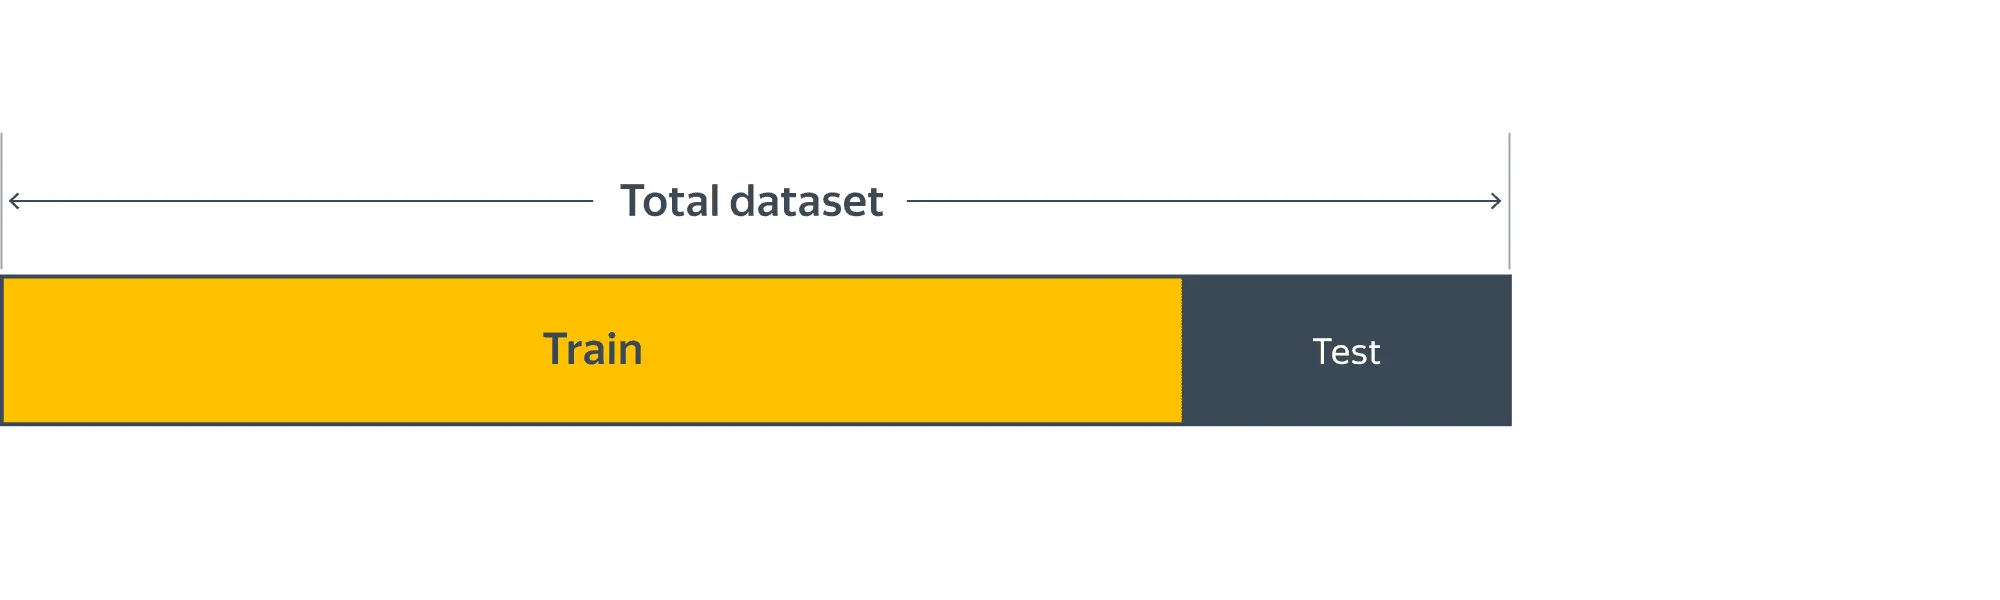
\includegraphics[width=\textwidth/2]{hold_out.png}
	\caption{Hold-out}
	\label{img:hold-out}
\end{figure}

\subsubsection{k-Fold}

Это самый распространенный метод кросс-валидации, в нём данные разбиваются на k подмножеств. Модель обучается k раз, каждый раз используя одно подмножество в качестве тестовой выборки, а остальные k-1 как тренировочные. В конце ошибкой модели считается либо средняя полученная ошибка по всем выборам тестового множества, либо вычисляется на отдельно отложенном валидационном множестве. Это позволяет использовать все доступные данные для обучения и тестирования, что особенно полезно в случаях, когда данные ограничены.

\begin{figure}[h]
	\centering
	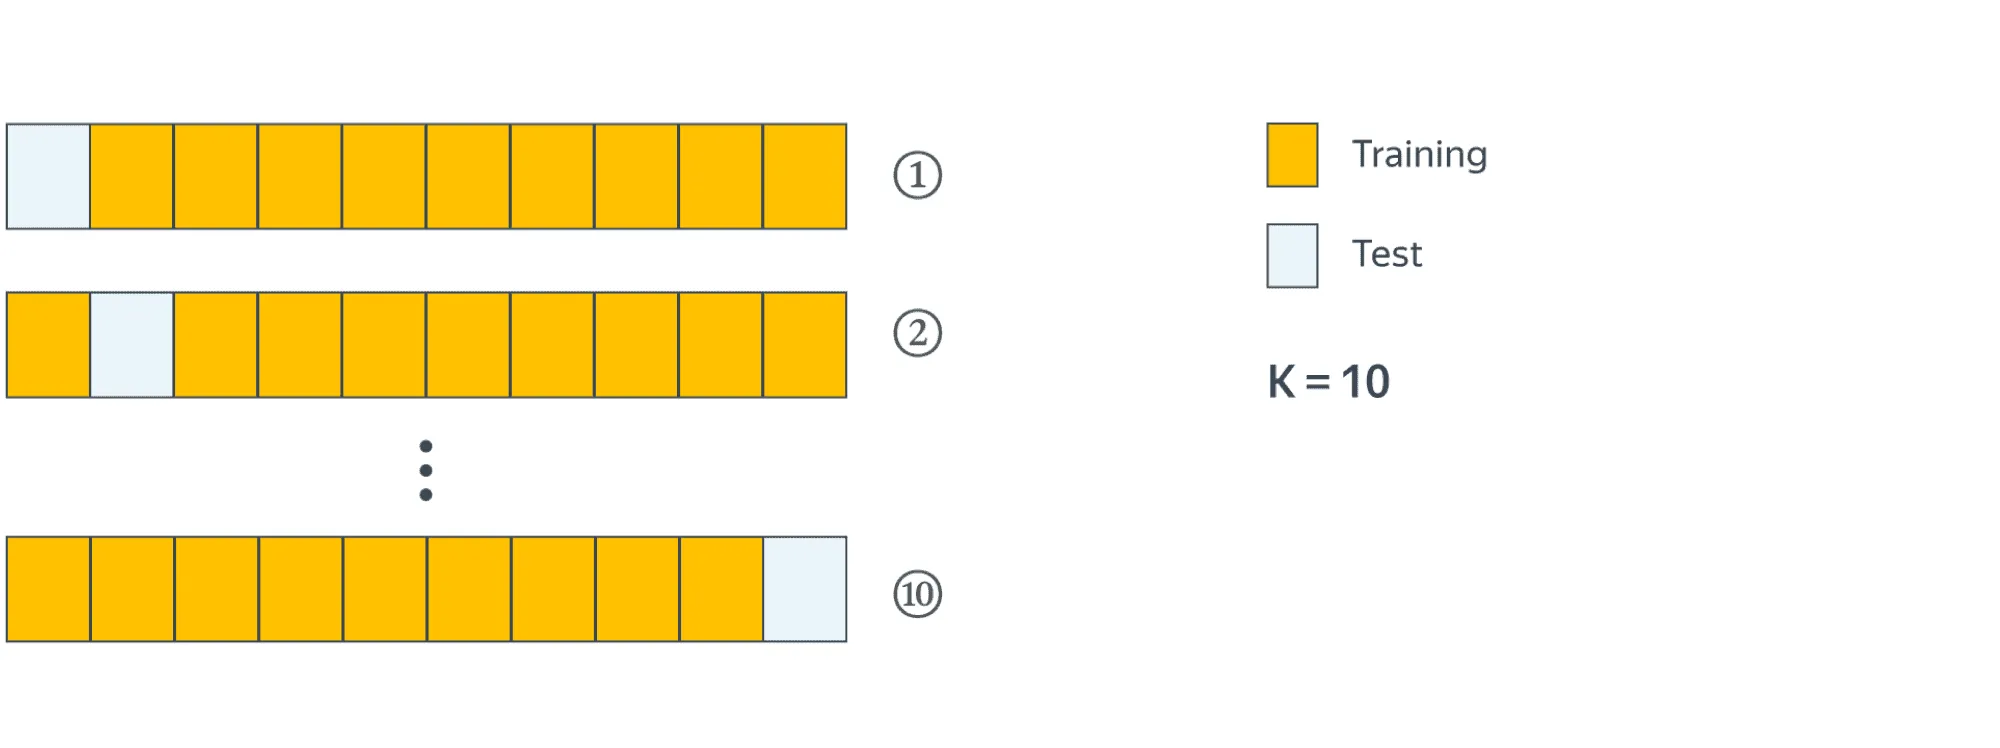
\includegraphics[width=\textwidth/2]{k-fold.png}
	\caption{k-Fold}
	\label{img:k-fold}
\end{figure}

Можно сделать вывод, что кросс-валидация помогает избежать переобучения и оптимизировать гиперпараметры моделей засчёт того, что модель много раз обучается и тестируется на разных подмножествах одних и тех же данных.

\subsection{Задачи (\href{https://education.yandex.ru/handbook/ml/article/kross-validaciya}{источник})}

\subsubsection{Задача 1}
Пример из практики Yandex.Research — как вы думаете, что не так с графиком обучения данной модели?

\begin{figure}[h]
	\centering
	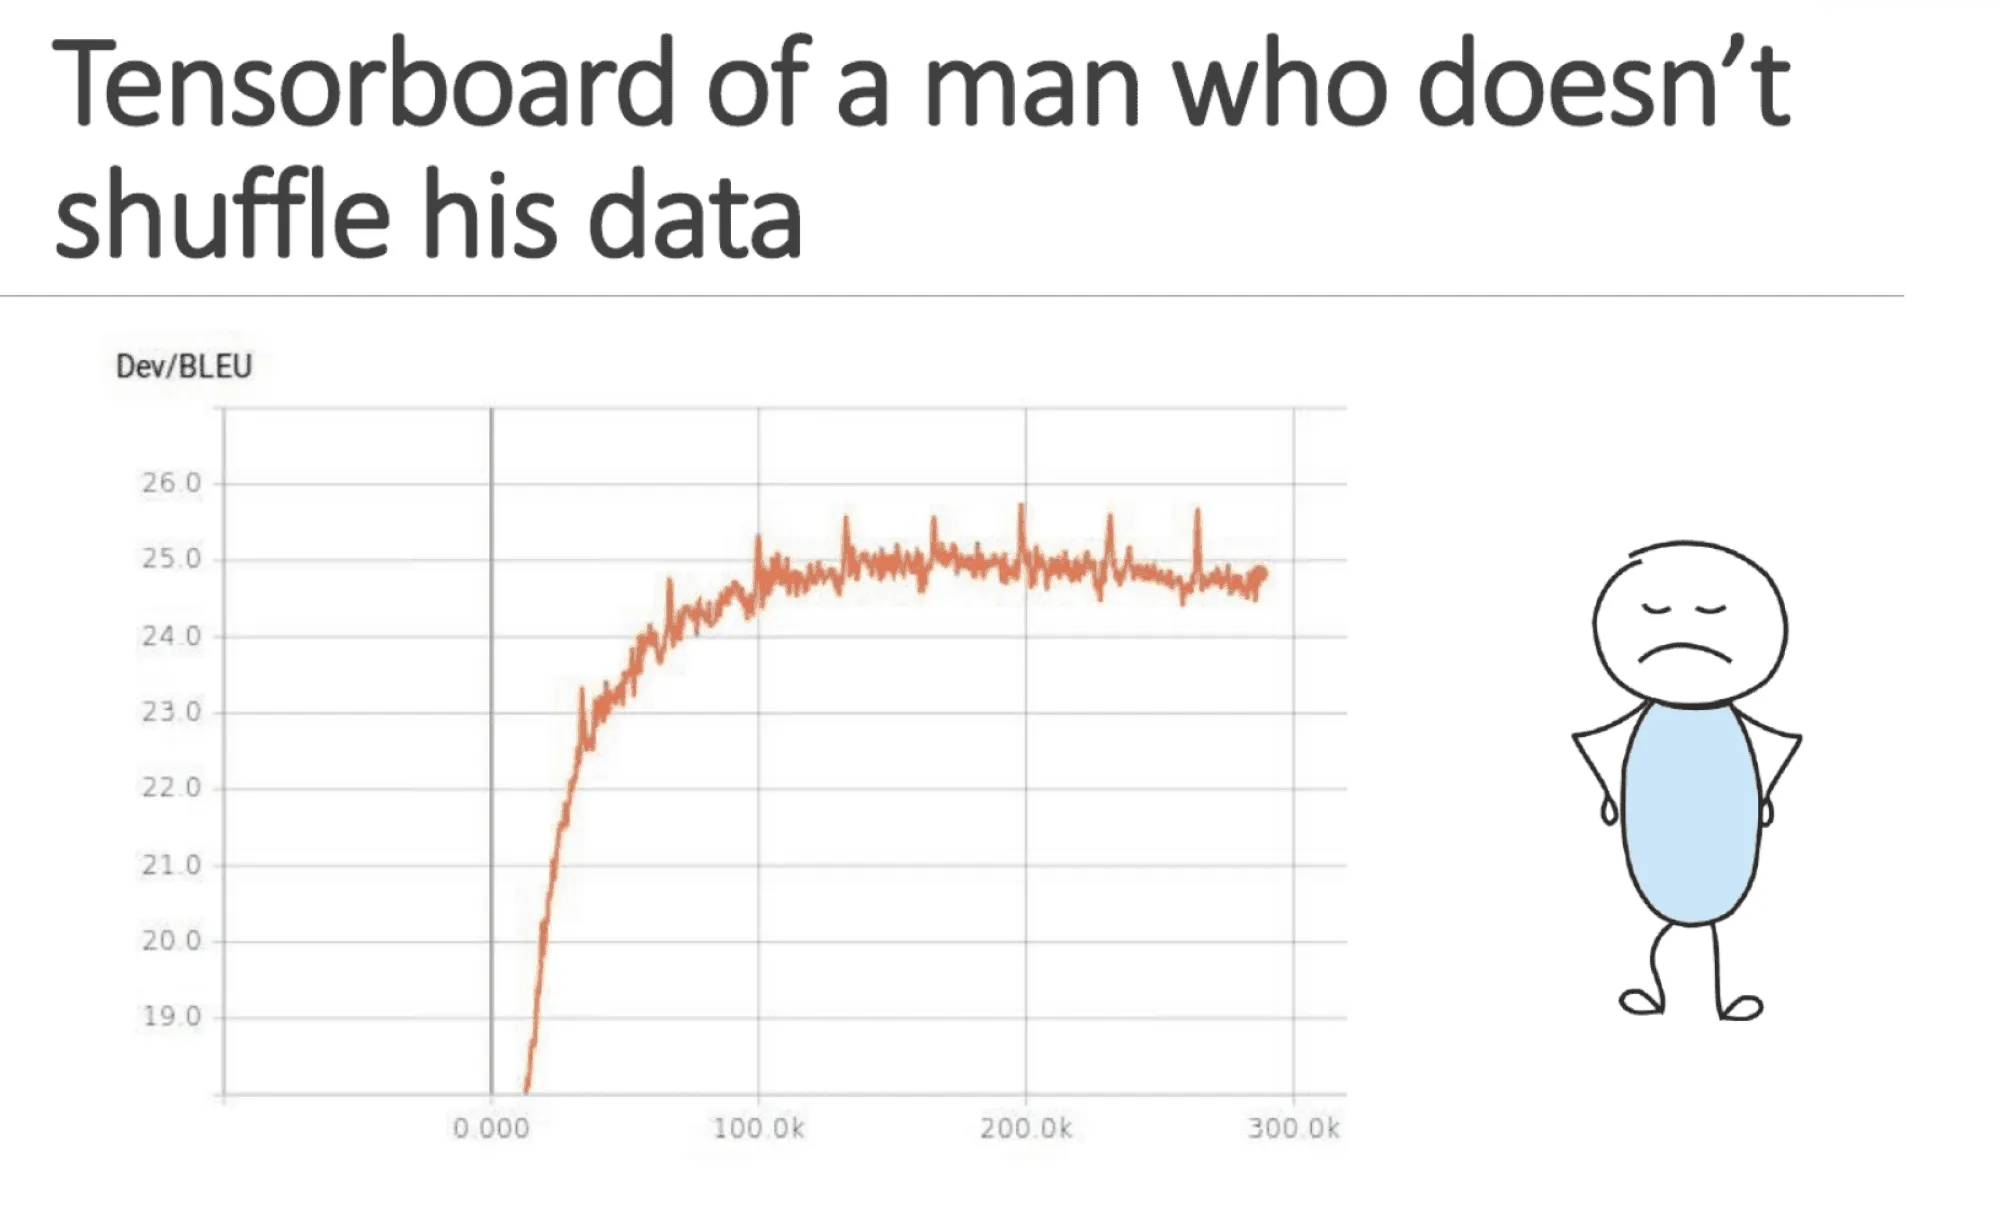
\includegraphics[width=\textwidth/2]{problem-1.png}
	\caption{Задача 1}
	\label{img:problem-1}
\end{figure}

\textit{Решение}
На графике видна периодичность по числу итераций! По большим пикам можно вычислить места, где проход по данным начался заново. Кроме того, график в конце ползёт вниз, что означает, что модель уже начала переобучаться, выучив последовательность данных на трейне и используя эту информацию больше, чем сами данные.

Если данные перемешать, то график обучения станет таким:

\begin{figure}[h]
	\centering
	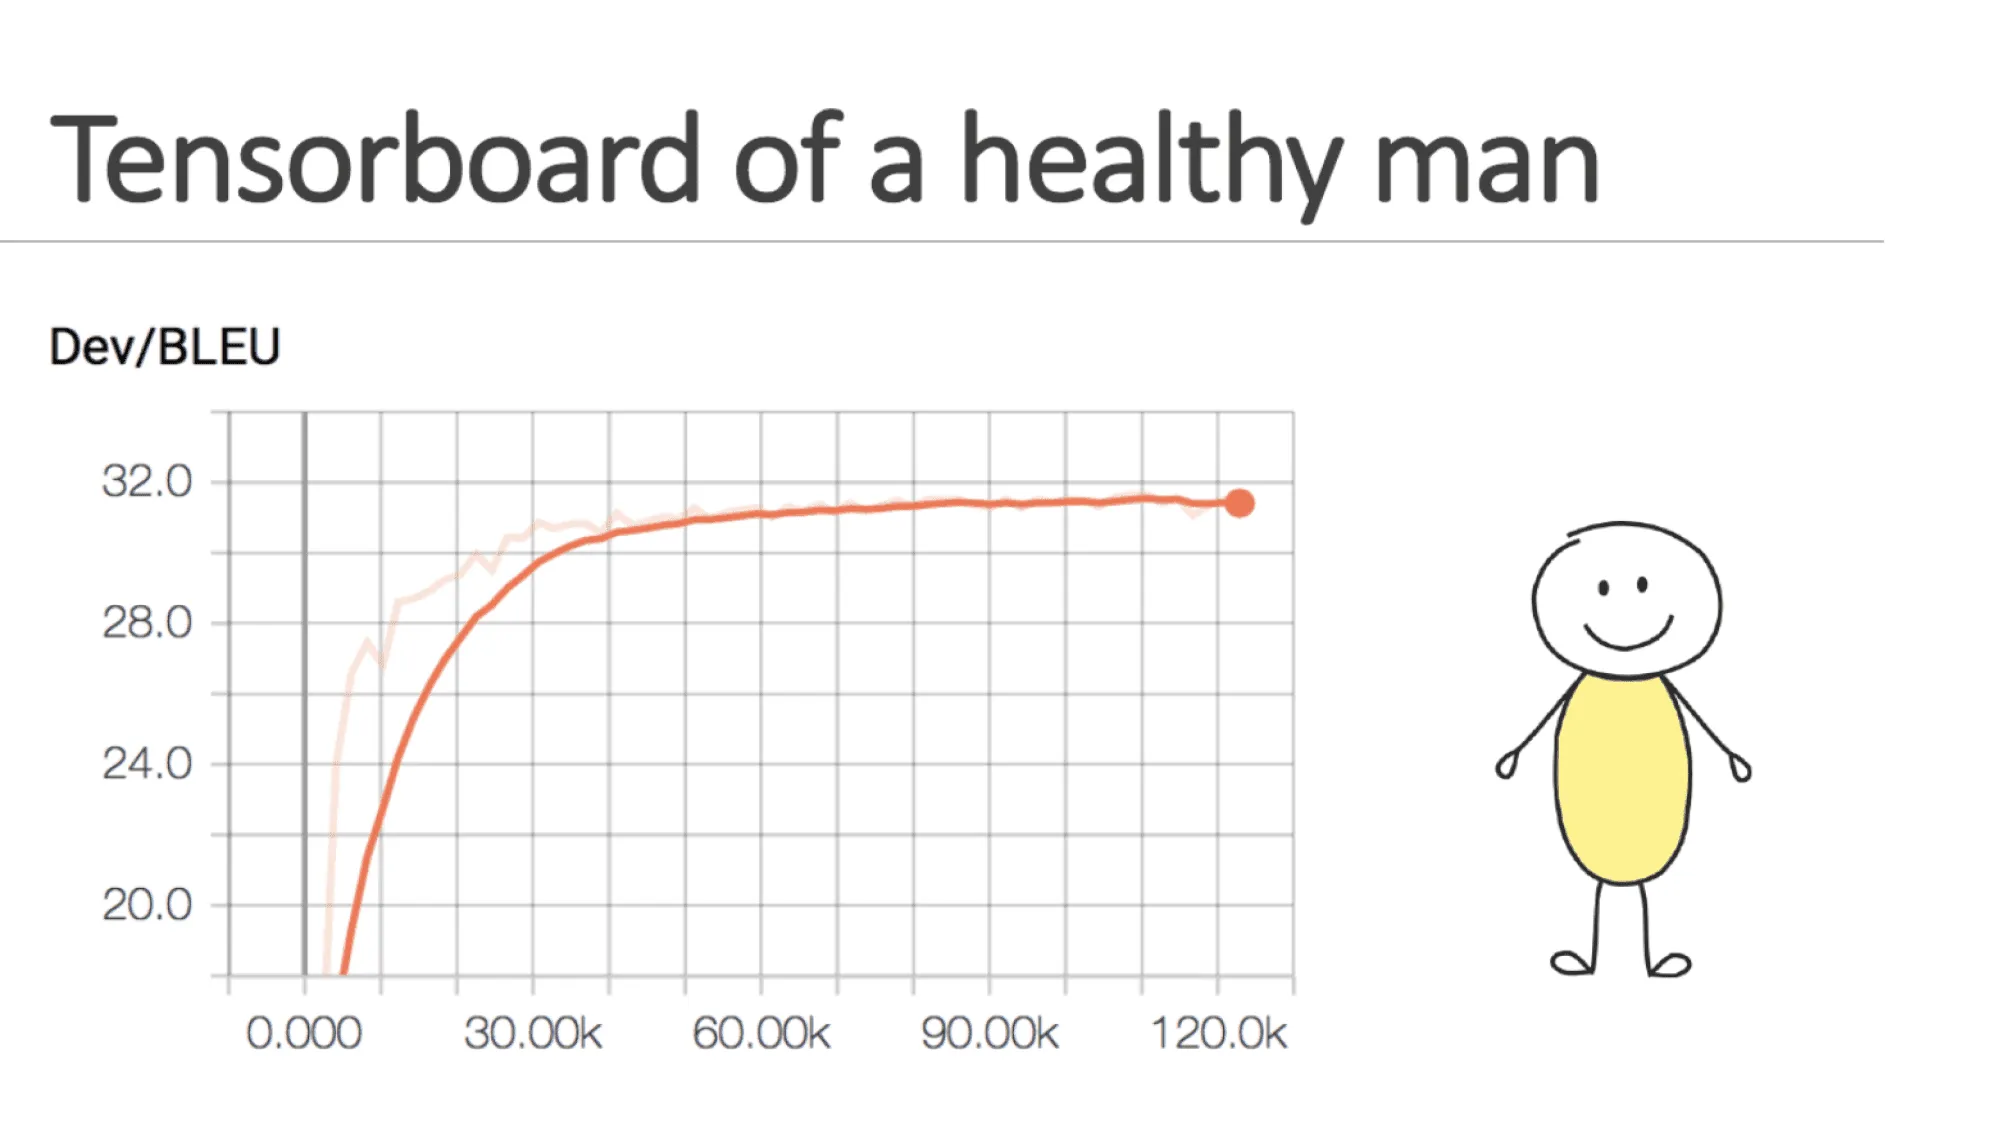
\includegraphics[width=\textwidth/2]{sol-1.png}
	\caption{Решение задачи 1}
	\label{img:sol-1}
\end{figure}

\subsubsection{Задача 2}

Пусть нужно обучить модель, которая должна предсказывать погоду. Есть исторические данные за последние 10 лет. Можно ли как обычно разделять данные на train и test, произвольно перемешивая их? Если нет, то как нужно разделять данные?

\textit{Решение}
Нет, так делать нельзя, потому что в таком случае у модели при обучении будет доступ к данным из <<будущего>>, которые он как раз и должна предсказывать, а это некорректно. Правильно будет разделить данные по времени: самые старые --- train, самые новые -- test.

\subsubsection{Задача 3}

А как сделать кросс-валидацию в условиях задачи 2?

\textit{Решение}

Нужно сделать несколько пар (train, test), но так, чтобы модель никогда не получала лишних данных из будущего. С учётом особенностей фолды в кросс-валидации для временных рядов располагаются вдоль временной оси так, как показано на следующей картинке:

\begin{figure}[h]
	\centering
	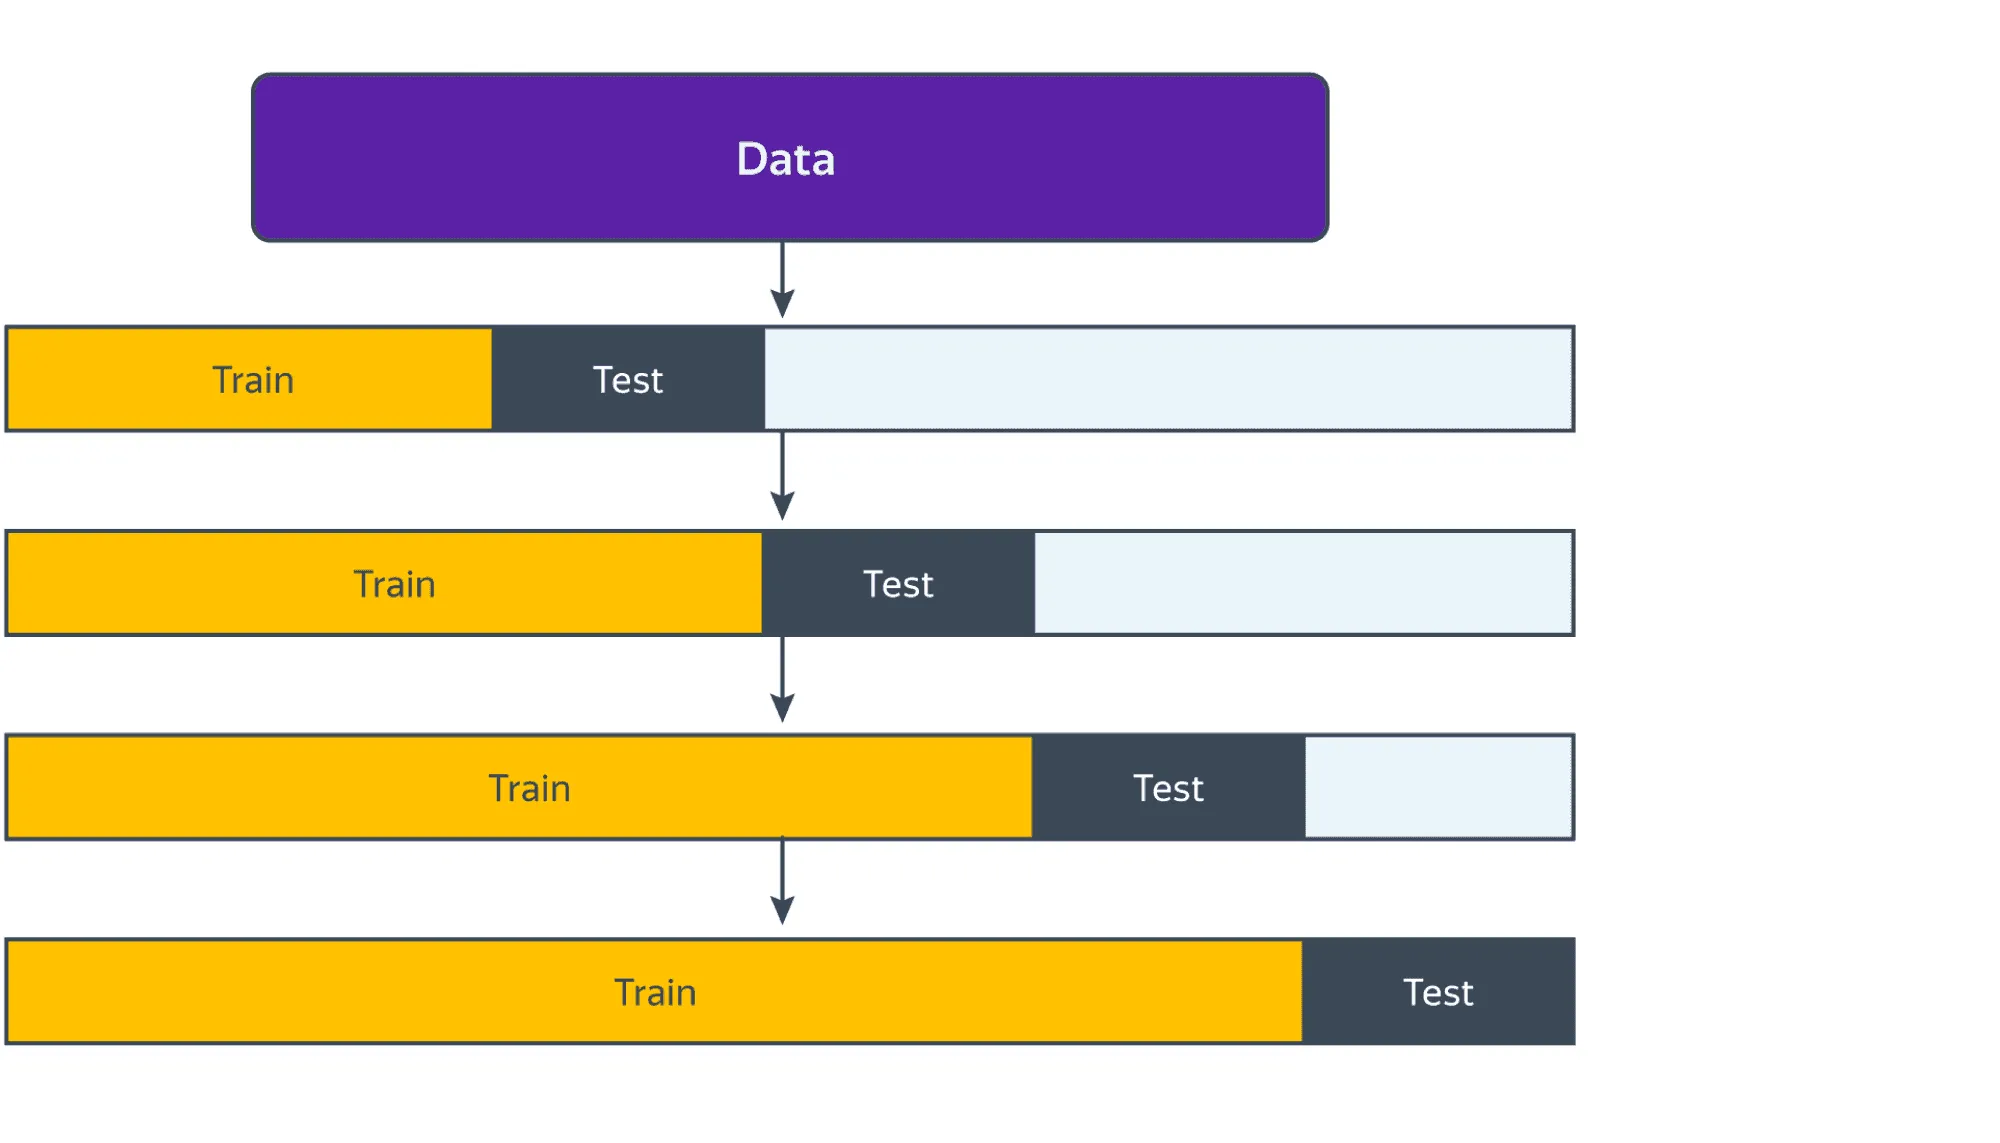
\includegraphics[width=\textwidth/2]{sol-3.png}
	\caption{Решение задачи 3}
	\label{img:sol-3}
\end{figure}


    \clearpage
    \chapter{Линейные методы классификации и регрессии}
    % !TeX spellcheck = ru_RU-Russian

\section{О регуляризации}

При решении задачи машинного обучения часто возникает проблема переобучения, при котором модель подстраивается под шум данных, что снижает ее обобщаю способность.
Один из методов борьбы с этим --- регуляризации, или же сокращение весов (англ.: weight decay). Данный метод добавляет штраф к функции потерь за сложность модели, в случае линейных моделей~--- штраф за большие веса коэффициентов. Регуляризация ограничивает пространство решений и делает модель более устойчивой к шуму, что увеличивает вероятность корректных предсказаний на новых данных. Пример, когда усложнение модели, путем добавления избыточных коэффициентов полиномиальной модели представлен на рис.~\ref{liner-reg-overfitting}.

\begin{figure}[ht]
	\centering
	\includegraphics[width=0.9\linewidth]{chapters/linear/pics/reg-overfitting.png}
	\caption{Иллюстрация проблемы переобучения для решения линейной задачи}
	\label{linear-reg-overfitting}
\end{figure}

В разделе~\ref{linear-reg-l1l2} рассмотрены основные методы регуляризации, применяемые в линейных моделях. Раздел~\ref{linear-reg-prob} описывает вероятностную трактовку причин возникновения регуляризации. Завершается глава разделом~\ref{linear-reg-task}, который содержит три теоретических задачи по теме регрессии.

\subsection{Гауссовский и лапласовский регуляризаторы}
\label{linear-reg-l1l2}

Гауссовский и лапласовский регуляризаторы представляют собой две разные техники регуляризации, которые используются для управления сложностью моделей и предотвращения переобучения. Они основаны на различных подходах к штрафованию весов модели.

\subsubsection{Лапласовский регуляризатор (L1 регуляризатор)}

Лапласовский (L1) регуляризатор использует сумму модулей значений весов модели в качестве штрафа. Формально новую функцию потерь можно записать следующим образом:
$L1 = L_0 + \lambda \sum_{i=1}^{n} |w_i|$,
где $L_0$ --- исходная функция потерь, $|w_i|$ --- абсолютные значения весов модели, $\lambda$ --- коэффициент регуляризации.
\noindent
Преимущества:
\begin{itemize}
	\item Лапласовский регуляризатор может приводить к обнулению некоторых весов, что делает модель более интерпретируемой и позволяет выделять наиболее важные признаки.
	\item Он может быть особенно полезен в задачах с высокой размерностью, где много признаков могут быть неинформативными.
\end{itemize}
Недостатки:
\begin{itemize}
	\item Оптимизация с использованием L1 регуляризации может быть более сложной и требовать специальных алгоритмов (например, координатного спуска или методов, основанных на субградиенте).
\end{itemize}

\subsubsection{Гауссовский регуляризатор (L2 регуляризатор)}

Гауссовский (L2) регуляризатор использует штраф в виде суммы квадратов весов модели. Формально новую функцию потерь можно записать следующим образом:
$L2 = L_0 + \lambda \sum_{i=1}^{n} w_i^2$,
где $L_0$ — исходная функция потерь (например, среднеквадратичная ошибка для задачи регрессии), $w_i$ — веса модели, $\lambda$ — коэффициент регуляризации, который контролирует величину штрафа.
Преимущества:
\begin{itemize}
	\item Гауссовский регуляризатор помогает сгладить веса, что делает модель более устойчивой к шуму в данных.
	\item Он способствует распределению весов по всем признакам, уменьшая вероятность того, что некоторые признаки будут доминировать.
\end{itemize}
Недостатки:
\begin{itemize}
	\item Может не приводить к полному обнулению весов, поэтому не всегда приводит к интерпретируемым моделям.
\end{itemize}

\subsubsection {Сравнений L1 и L2 регуляризаторов}

Выбор между гауссовским и лапласовским регуляризаторами зависит от конкретной задачи и целей (сравнение см. в таблице~\ref{linear-reg-comp}). Если важна интерпретируемость модели и выделение значимых признаков, то стоит рассмотреть L1 регуляризацию. Если же цель — улучшить общее качество модели без сильного сокращения количества признаков, то L2 регуляризация может быть предпочтительнее. Это связано с тем, что в L2 регуляризации за счет возведения в квадрат значений весов вклад нулевого веса и просто малого веса неразличим на при наличии других выделенных признаков с весами порядка или более единицы. Таким образом, L2 регуляризация, в отличии от L1 не стремится обнулить коэффициенты, что снижает интерпретируемость модели. Однако квадратичная функция является гладкой, поэтому лучше поддается вычислительным методам оптимизации.

\begin{table}[ht]
	\caption{Сравнение L1 и L2 регуляризаторов}
	\label{linear-reg-comp}
	\begin{tabular}{l|l|l}
		Характеристика & Лапласовский (L1) & Гауссовский (L2) \\
		\hline
		Штраф & Сумма абсолютных значений весов & Сумма квадратов весов \\
		Эффект на веса & Обнуление (спарсность) & Сглаживание \\
		Интерпретируемость & Выше & Меньше \\
		Оптимизация & Сложнее & Легче
	\end{tabular}
\end{table}

В ситуациях используется комбинация обоих методов регуляризации. Для этого вводится дополнительный гиперпараметр $\alpha$~--- доля первой нормы в штрафе за вес. Получается так называемая эластичная сеть (англ.: elastic net). В таком случае:
$L = L_0 + \lambda [\alpha \sum_{i=1}^{n} |w_i| + (1 - \alpha) \sum_{i=1}^{n} w_i^2]$. Данный подход позволяет учесть особенности двух подходов, однако усложняет модель.

\subsection {Вероятностная интерпретация регуляризации}
\label{linear-reg-prob}

В первом рассмотрении регуляризацию можно рассматриваться как введение априорной информации о параметрах модели. Рассмотрим вводимые предположения:
\begin{itemize}
	\item в случае L1 регуляризации мы предполагаем, что многие веса могут быть равны нулю, это соответствует идее о том, что истинная модель простая и присутствуют лишние признаки;
	\item в случае L2~--- веса распределены вблизи общего малого среднего значения, это отражает предположение о том, что все признаки вносят сопоставимый вклад в предсказание.
\end{itemize}
\noindent
Описанным выше предположениям о весах соответствуют экспоненциальное и нормальное распределения (см. рис.~\ref{linear-reg-distribution}). Рассмотрим их влияние на штраф и функцию потерь.

\begin{figure}[ht]
	\centering
	\includegraphics[width=0.9\linewidth]{chapters/linear/pics/reg-distributions.png}
	\caption{Сравнение экспоненциального и нормального распределений}
	\label{linear-reg-distribution}
\end{figure}

\subsubsection {L1 регуляризация}

предполагает, что веса $w_j$ распределены по лапласовскому закону (или двойному экспоненциальному распределению), $w_j - Laplace(0, b)$.

\subsubsection{L2 регуляризация}

предполагает, что веса модели $w_j$ имеют нормальное распределение с нулевым средним и некоторой дисперсией $\sigma^2$. Это можно записать как $w_j - N(0, \sigma^2)$.

\subsection {Задачи}
\label{linear-reg-task}


\subsubsection{Вопрос 1}
\noindent Как изменение коэффициента $\lambda$ влияет на величину весов $w_j$?

\textbf{L1 регуляризация}

\noindent При увеличении $\lambda$ происходит обнулению некоторых весов $w_j$. Это приводит к тому, что с увеличением $\lambda$ количество ненулевых весов уменьшается, что может помочь в отборе признаков и упрощении модели.

\textbf{L2 регуляризация}

\noindent При увеличении $\lambda$ происходит увеличение штрафа за большие значения весов. Это приводит к уменьшению величины весов $w_j$ (все веса стремятся к нулю), что помогает избежать переобучения. В случае $\lambda$ = 0 модель не имеет регуляризации, и веса могут принимать любые значения, что может привести к переобучению.

\subsubsection{Вопрос 2}
\noindent Какова геометрическая интерпретация регуляризации в пространстве весов?

\begin{figure}[ht]
	\centering
	\includegraphics[width=0.9\linewidth]{chapters/linear/pics/reg-geom.png}
	\caption{Геометрическая интерпретация регуляризации в пространстве весов}
	\label{linear-reg-geom}
\end{figure}

\textbf{L1 регуляризация}

\noindent Геометрически L1 регуляризация создает ромбовидные (или параллелепипедные) области в пространстве весов. Оптимальные веса находятся на вершинах этих ромбов, что приводит к обнулению некоторых весов и, следовательно, к отбору признаков.

$L1(w_1,w_2) = const <=> |w_1|+|w_2| = const$

\textbf{L2 регуляризация}

\noindent Геометрически L2 регуляризация создает сферу (или гиперсферу) в пространстве весов, внутри которой минимизируется функция потерь. Это означает, что оптимальные веса будут находиться на поверхности этой сферы, что приводит к сглаживанию и уменьшению значений весов.

$L2(w_1,w_2) = const <=> w_1^2+w_2^2 = const$

\subsubsection{Вопрос 3}
\noindent Какие особенности признаков компенсируют регуляризации?

\textbf{L1 регуляризация}

\noindent Используя L1 регуляризацию, можно обнулить веса для менее значимых признаков. После обучения модели можно проанализировать ненулевые веса и оставить только те признаки, которые имеют значимые коэффициенты, тем самым осуществляя отбор признаков.

\textbf{L2 регуляризация}

\noindent L2 регуляризация помогает сгладить веса при наличии мультиколлинеарности, уменьшая их величину и тем самым снижая влияние коррелирующих признаков. Это позволяет избежать чрезмерного увеличения весов для сильно коррелирующих признаков.

\section*{Основная идея}

Градиентные методы --- это широкий класс оптимизационных алгоритмов, используемых не только в машинном обучении. Здесь градиентный подход будет рассмотрен в качестве способа подбора вектора синаптических весов \( w \) в линейном классификаторе. Пусть \( y^*: \, X \to Y \) — целевая зависимость, известная только на объектах обучающей выборки: \( X^l = (x_i, y_i)_{i=1}^l \), где \( y_i = y^*(x_i) \).

Найдём алгоритм \( a(x, w) \), аппроксимирующий зависимость \( y^* \). В случае линейного классификатора искомый алгоритм имеет вид:
$$ a(x, w) = \varphi\left(\sum_{j=1}^n w_j x^j - w_0\right), $$
где \( \varphi(z) \) играет роль функции активации (в простейшем случае можно положить \( \varphi(z) = \operatorname{sign}(z) \)).

Согласно принципу минимизации эмпирического риска, для этого достаточно решить оптимизационную задачу:
$$ Q(w) = \sum_{i=1}^l L(a(x_i, w), y_i) \to \min_w, $$
где \( L(a, y) \) — заданная функция потерь.

Для минимизации применим метод градиентного спуска (gradient descent). Это пошаговый алгоритм, на каждой итерации которого вектор \( w \) изменяется в направлении наибольшего убывания функционала \( Q \) (то есть в направлении антиградиента):
$$ w := w - \eta \nabla Q(w), $$
где \( \eta \) — положительный параметр, называемый темпом обучения (learning rate).

\subsection*{Основные подходы к реализации градиентного спуска}
\begin{enumerate}
    \item \textbf{Пакетный (batch):} на каждой итерации обучающая выборка просматривается целиком, и только после этого изменяется \( w \). Этот подход требует больших вычислительных затрат.
    \item \textbf{Стохастический (stochastic/online):} на каждой итерации из обучающей выборки случайным образом выбирается один объект. Таким образом, вектор \( w \) настраивается на каждый вновь выбираемый объект.
\end{enumerate}

\subsection*{Алгоритм Stochastic Gradient (SG)}
\textbf{Вход:}
\begin{itemize}
    \item \( X^l \) --- обучающая выборка;
    \item \( \eta \) --- темп обучения;
    \item \( \lambda \) --- параметр сглаживания функционала \( Q \).
\end{itemize}

\textbf{Выход:} Вектор весов \( w \)

\textbf{Тело алгоритма:}
\begin{enumerate}
    \item Инициализировать веса \( w_j \), \( j = 0, \dots, n \);
    \item Инициализировать текущую оценку функционала: \( Q := \sum_{i=1}^l L(a(x_i, w), y_i) \);
    \item Повторять:
    \begin{enumerate}
        \item выбрать объект \( x_i \) из \( X^l \) (например, случайным образом);
        \item вычислить выходное значение алгоритма \( a(x_i, w) \) и ошибку: \( \varepsilon_i := L(a(x_i, w), y_i) \);
        \item сделать шаг градиентного спуска:
        $$ w := w - \eta L_a^\prime (a(x_i, w), y_i) \varphi^\prime (\langle w, x_i \rangle)x_i; $$
        \item оценить значение функционала:
        $$ Q := (1 - \lambda)Q + \lambda\varepsilon_i; $$
    \end{enumerate}
    пока значение \( Q \) не стабилизируется и/или веса \( w \) не перестанут изменяться.
\end{enumerate}

\subsection*{Порядок выбора объектов}
В случае стохастического градиентного спуска объекты следует выбирать случайным образом, однако существуют эвристики, направленные на улучшение сходимости:
\begin{itemize}
    \item Перемешивание (shuffling): случайно выбирать объекты, попеременно из разных классов. Идея в том, что объекты из разных классов менее "похожи", чем объекты одного класса, поэтому вектор \( w \) будет сильнее изменяться.
    \item Можно выбирать объект с вероятностью, обратно пропорциональной величине ошибки на объекте. Следует учитывать, что такая эвристика делает метод чувствительным к шумам.
\end{itemize}

\subsection*{Способы инициализации весов}
\begin{enumerate}
    \item Инициализация вектора \( w \) нулями.
    \item \( w_j := \operatorname{rand}\left(-\frac{1}{n}, \frac{1}{n}\right) \), где \( n \) — размерность пространства признаков.
    \item Решение исходной оптимизационной задачи при условии статистически независимых признаков, линейной функции активации (\( \varphi \)) и квадратичной функции потерь (\( L \)):
    $$ w_j := \frac{\langle y, f_j \rangle}{\langle f_j, f_j \rangle}. $$
\end{enumerate}

\subsection*{Параметр сглаживания}
Для оценки функционала \( Q \) на каждой итерации используется его приближённое значение по методу экспоненциального сглаживания, откуда \( \lambda \) лучше брать порядка \( \frac{1}{l} \).

\subsection*{Известные частные случаи алгоритма}
Метод SG (при соответствующем выборе функций активации и потерь) является обобщением следующих эвристик подбора \( w \) и алгоритмов классификации:
\begin{itemize}
    \item Адаптивный линейный элемент (Adalines);
    \item Правило Хэбба;
    \item Алгоритм \( k \)-средних (K-Means);
    \item Learning Vector Quantization (LVQ).
\end{itemize}

\subsection*{Преимущества SG}
\begin{itemize}
    \item Метод подходит для динамического (online) обучения.
    \item Алгоритм способен обучаться на избыточно больших выборках.
    \item Различные стратегии обучения позволяют адаптировать алгоритм для задач с избыточной или небольшой выборкой.
\end{itemize}

\subsection*{Недостатки SG и способы их устранения}
\begin{itemize}
    \item Возможны проблемы сходимости. Для борьбы с этим применяют технику встряхивания коэффициентов.
    \item При высокой размерности пространства признаков \( n \) и/или малой длине выборки \( l \) возможно переобучение. Для борьбы с этим применяют метод сокращения весов:
    $$ Q_{\tau}(w) = Q(w) + \frac{\tau}{2}||w||^2. $$
    Тогда правило обновления весов принимает вид:
    $$ w := w(1 - \eta \tau) - \eta \nabla Q(w). $$
    \item При больших значениях \( \langle w, x_i \rangle \) значение \( \varphi^\prime \) может становиться близким к нулю. Для предотвращения этого состояния вводят нормализацию признаков:
    $$ x^j := \frac{x^j - x_{\min}^j}{x_{\max}^j - x_{\min}^j}, \quad j = 1, \dots, n, $$
    где \( x_{\min}^j, x_{\max}^j \) — минимальное и максимальное значения признака \( j \)-го признака. Регуляризация, такая как weight decay, также помогает избежать "паралича".
\end{itemize}

\subsection*{Сходимость алгоритма}
Сходимость гарантируется при выпуклой функции \( Q(w) \) и выполнении следующих условий:
$$ \eta_t \xrightarrow{t \to \infty} 0, \quad \sum_{t=1}^{\infty} \eta_t = \infty, \quad \sum_{t=1}^{\infty} \eta_t^2 < \infty. $$
Например, можно положить \( \eta_t = \frac{\eta_0}{t} \), хотя на практике это не всегда удачно.

\section*{Задачи}

\subsection*{Задача 1: Доказать сходимость алгоритма при условиях выше}

\textbf{Решение:}

\begin{enumerate}
    \item \textbf{Выпуклость функции:} Поскольку \( Q(w) \) выпукла, мы можем использовать свойства выпуклых функций. Для любого \( w \) и \( w^* \) (где \( w^* \) — точка минимума функции \( Q \)) выполняется неравенство:
    $$ Q(w) \geq Q(w^*) + \nabla Q(w^*)^T (w - w^*). $$

    \item \textbf{Итерация метода стохастического градиента:} Обновление весов в SGD задается следующим образом:
    $$ w_{t+1} = w_t - \eta_t \nabla Q(w_t; \xi_t), $$
    где \( \xi_t \) — случайная переменная, представляющая выборку данных на итерации \( t \).

    \item \textbf{Анализ изменения функции:} Мы можем оценить изменение функции \( Q \) на каждой итерации:
    $$ Q(w_{t+1}) \leq Q(w_t) + \nabla Q(w_t; \xi_t)^T (w_{t+1} - w_t) + \frac{L}{2} \|w_{t+1} - w_t\|^2, $$
    где \( L \) — константа Липшица для градиента \( \nabla Q \).

    Подставляя обновление:
    $$ Q(w_{t+1}) \leq Q(w_t) - \eta_t \nabla Q(w_t; \xi_t)^T \nabla Q(w_t) + \frac{L}{2} \eta_t^2 \|\nabla Q(w_t; \xi_t)\|^2. $$

    \item \textbf{Суммирование изменений:} Суммируя по всем итерациям, мы получаем:
    $$ \sum_{t=1}^{T} Q(w_{t+1}) - Q(w_1) \leq -\sum_{t=1}^{T} \eta_t \nabla Q(w_t; \xi_t)^T \nabla Q(w_t) + \sum_{t=1}^{T} \frac{L}{2} \eta_t^2 \|\nabla Q(w_t; \xi_t)\|^2. $$

    \item \textbf{Использование условий:} Условия \( \sum_{t=1}^{\infty} \eta_t = \infty \) и \( \sum_{t=1}^{\infty} \eta_t^2 < \infty \) позволяют нам сделать вывод о том, что:
    \begin{itemize}
        \item Сумма шагов обучения стремится к бесконечности, что означает, что веса \( w_t \) будут продолжать обновляться.
        \item Сумма квадратов шагов обучения конечна, что позволяет контролировать величину изменений на каждой итерации.
    \end{itemize}

    \item \textbf{Сходимость к минимуму:} В результате, при условии, что \( Q(w) \) выпукла, и учитывая условия на шаги обучения, мы можем утверждать, что последовательность \( w_t \) будет сходиться к некоторой точке \( w^* \), которая является минимумом функции \( Q(w) \).
\end{enumerate}

Таким образом, метод стохастического градиента сходится к минимуму выпуклой функции \( Q(w) \) при выполнении заданных условий.

\subsection*{Задача 2: Оценка вариации градиента}

\textbf{Условие:} Пусть \( \xi_1, \xi_2, \ldots, \xi_n \) — независимые и одинаково распределённые (i.i.d.) случайные переменные, представляющие собой выборки из обучающего набора. Рассмотрим стохастический градиент \( \nabla L(\theta; \xi_t) \).

\textbf{Задача:} Доказать, что математическое ожидание стохастического градиента совпадает с истинным градиентом функции потерь:
\[
\mathbb{E}[\nabla L(\theta; \xi_t)] = \nabla L(\theta)
\]
и оценить дисперсию \( \operatorname{Var}(\nabla L(\theta; \xi_t)) \) в зависимости от размера выборки \( n \).

\subsection*{Доказательство}

\begin{enumerate}
    \item \textbf{Определение стохастического градиента:} Пусть \( L(\theta) \) — функция потерь, зависящая от параметров \( \theta \) и от выборки \( \xi \). Мы можем записать функцию потерь как среднее значение по всем данным:
    $$ L(\theta) = \frac{1}{n} \sum_{i=1}^{n} l(\theta; x_i, y_i), $$
    где \( l(\theta; x_i, y_i) \) — функция потерь для примера \( (x_i, y_i) \).

    \item \textbf{Истинный градиент:} Тогда истинный градиент функции потерь можно выразить как:
    $$ \nabla L(\theta) = \frac{1}{n} \sum_{i=1}^{n} \nabla l(\theta; x_i, y_i). $$

    \item \textbf{Математическое ожидание стохастического градиента:} Теперь рассмотрим стохастический градиент:
    $$ \nabla L(\theta; \xi_t) = \nabla l(\theta; \xi_t), $$
    где \( \xi_t \) — случайная выборка. Поскольку \( \xi_t \) выбирается из одного из \( n \) примеров, математическое ожидание стохастического градиента будет:
    \[
    \mathbb{E}[\nabla L(\theta; \xi_t)] = \mathbb{E}[\nabla l(\theta; \xi_t)] = \frac{1}{n} \sum_{i=1}^{n} \nabla l(\theta; x_i, y_i) = \nabla L(\theta).
    \]
    Таким образом, мы доказали, что:
    \[
    \mathbb{E}[\nabla L(\theta; \xi_t)] = \nabla L(\theta).
    \]

    \item \textbf{Оценка дисперсии:} Теперь найдём дисперсию стохастического градиента:
    \[
    \operatorname{Var}(\nabla L(\theta; \xi_t)) = \mathbb{E}[(\nabla L(\theta; \xi_t) - \mathbb{E}[\nabla L(\theta; \xi_t)])^2].
    \]
    Подставим выражение для стохастического градиента:
    \[
    \operatorname{Var}(\nabla L(\theta; \xi_t)) = \mathbb{E}[(\nabla l(\theta; \xi_t) - \nabla L(\theta))^2].
    \]
    Поскольку \( \xi_t \) является случайным выбором, мы можем использовать свойства дисперсии. Для \( n \) независимых и одинаково распределённых (i.i.d.) выборок дисперсия стохастического градиента будет уменьшаться с увеличением размера выборки:
    $$ \operatorname{Var}(\nabla L(\theta; \xi_t)) = \frac{1}{n} \operatorname{Var}(l(\theta; x, y)), $$
    где \( (x, y) \) — случайная выборка из обучающего набора. Это означает, что дисперсия стохастического градиента уменьшается с увеличением размера выборки \( n \).
\end{enumerate}

\subsection*{Задача 3: Регуляризация и стохастический градиент}

\subsection*{Условие}
Рассмотрим функцию потерь с L2-регуляризацией:
$$ L(\theta) = \frac{1}{n} \sum_{i=1}^{n} l(\theta; x_i, y_i) + \frac{\lambda}{2} \|\theta\|^2 $$
где \( l(\theta; x_i, y_i) \) — функция потерь для примера \( (x_i, y_i) \), а \( \lambda \) — коэффициент регуляризации.

\subsection*{Задача}
Обосновать, как регуляризация влияет на сходимость метода стохастического градиента, и показать, что использование регуляризации может помочь избежать переобучения, уменьшая значение функции потерь на валидационном наборе.

\subsection*{Влияние регуляризации на сходимость метода стохастического градиента}
\begin{enumerate}
    \item \textbf{Сглаживание функции потерь:}
    \begin{itemize}
        \item Добавление L2-регуляризации к функции потерь делает её более гладкой и выпуклой. Это связано с тем, что регуляризационный член \( \frac{\lambda}{2} \|\theta\|^2 \) добавляет "наказание" за большие значения параметров, что предотвращает резкие изменения градиента.
        \item Гладкость функции потерь способствует более стабильному обновлению параметров при использовании стохастического градиента. Это означает, что обновления параметров будут более предсказуемыми и менее подвержены шуму, что улучшает сходимость алгоритма.
    \end{itemize}

    \item \textbf{Уменьшение переобучения:}
    \begin{itemize}
        \item Регуляризация способствует уменьшению значений параметров модели, что, в свою очередь, снижает сложность модели. Это позволяет избежать переобучения, когда модель слишком точно подстраивается под тренировочные данные, включая шум.
        \item В результате, при использовании регуляризации, модель будет лучше обобщаться на новых данных, что выражается в меньшем значении функции потерь на валидационном наборе.
    \end{itemize}
\end{enumerate}

\subsection*{Доказательство эффекта регуляризации на валидационном наборе}
\begin{enumerate}
    \item \textbf{Функция потерь на валидационном наборе:}
    \begin{itemize}
        \item Пусть \( L_{val}(\theta) \) — функция потерь на валидационном наборе. При использовании регуляризации, мы можем записать:
        $$ L_{val}(\theta) = \frac{1}{m} \sum_{j=1}^{m} l(\theta; x_j, y_j) + \frac{\lambda}{2} \|\theta\|^2 $$
        где \( m \) — количество примеров в валидационном наборе.
    \end{itemize}

    \item \textbf{Сравнение значений функции потерь:}
    \begin{itemize}
        \item Без регуляризации, модель может иметь высокую функцию потерь на валидационном наборе из-за переобучения. При добавлении L2-регуляризации, даже если функция потерь на тренировочном наборе остаётся низкой, регуляризация помогает поддерживать значение функции потерь на валидационном наборе на более низком уровне.
    \end{itemize}

    \item \textbf{Кросс-валидация для выбора \( \lambda \):}
    \begin{itemize}
        \item Оптимальное значение \( \lambda \) можно выбрать с помощью кросс-валидации. Это позволяет находить компромисс между сложностью модели и её обобщающей способностью, что в конечном итоге приводит к меньшему значению функции потерь на валидационном наборе.
    \end{itemize}
\end{enumerate}

\subsection*{Заключение по задаче 3}
Регуляризация, особенно L2-регуляризация, играет ключевую роль в улучшении сходимости метода стохастического градиента и в предотвращении переобучения модели. Она помогает сделать функцию потерь более гладкой и выпуклой, что способствует стабильности обновлений параметров. В результате, использование регуляризации приводит к лучшему обобщению модели и снижению значения функции потерь на валидационном наборе, что является важным аспектом при разработке надёжных моделей в машинном обучении.

\section*{Линейный дискриминантный анализ (LDA)}

Линейный дискриминантный анализ (LDA) — это статистический метод для решения задач классификации, который используется для поиска линейных комбинаций признаков, наиболее эффективно разделяющих два или более классов. Основной задачей LDA является минимизация внутриклассовой дисперсии и максимизация межклассовой дисперсии, что позволяет лучше различать классы на основе их характеристик.

\subsection*{Предположения LDA}

LDA предполагает следующие условия для классов данных:
\begin{enumerate}
    \item \textbf{Нормальность распределений.} Признаки \( x \in \mathbb{R}^m \) для каждого класса \( C_k \) распределены нормально с параметрами: средним вектором \( \mu_k \in \mathbb{R}^m \) и ковариационной матрицей \( \Sigma_k \in \mathbb{R}^{m \times m} \).
    \item \textbf{Одинаковые ковариационные матрицы.} Все классы имеют одинаковую ковариационную матрицу \( \Sigma \), что значительно упрощает задачу классификации, так как для построения линейной границы между классами используется одна и та же матрица ковариаций.
\end{enumerate}

Согласно этим предположениям, распределение признаков в каждом классе можно выразить через многомерное нормальное распределение:
\[
P(x | C_k) = \frac{1}{(2\pi)^{m/2} |\Sigma|^{1/2}} \exp\left( -\frac{1}{2} (x - \mu_k)^T \Sigma^{-1} (x - \mu_k) \right),
\]
где \( \mu_k \) — средний вектор признаков для класса \( C_k \), а \( \Sigma \) — ковариационная матрица, одинаковая для всех классов.

\subsection*{Задача LDA}

Цель LDA заключается в нахождении линейного классификатора, который разделяет классы с минимальной ошибкой. Для этого LDA ищет линейную функцию от признаков \( x \) вида:
\[
\delta(x) = w^T x + b,
\]
где \( w \) — вектор весов, \( b \) — смещение. Классы разделяются гиперплоскостью, заданной уравнением:
\[
w^T x + b = 0.
\]

Классификация основывается на выборе того класса, для которого значение \( \delta(x) \) наибольшее:
\[
\hat{y} = \text{sign}(w^T x + b).
\]

\subsection*{Вывод классификатора LDA}

Для решения задачи классификации методом LDA необходимо максимизировать правдоподобие для наблюдаемых данных, предполагая, что каждый класс имеет нормальное распределение с одинаковыми ковариационными матрицами. Рассмотрим два класса \( C_1 \) и \( C_2 \). Обозначим средние векторы классов как \( \mu_1 \) и \( \mu_2 \), а ковариационную матрицу как \( \Sigma \).

В соответствии с теоремой Байеса, для каждого класса вероятность \( P(C_k | x) \) вычисляется как:
\[
P(C_k | x) = \frac{P(x | C_k) P(C_k)}{P(x)}.
\]
Для того чтобы классифицировать объект \( x \), необходимо выбрать класс с наибольшей апостериорной вероятностью. Так как \( P(x) \) не зависит от класса, задача сводится к сравнению правдоподобий:
\[
P(C_1 | x) > P(C_2 | x) \quad \text{или} \quad \log P(C_1 | x) > \log P(C_2 | x).
\]

Подставив выражения для \( P(x | C_1) \) и \( P(x | C_2) \), получаем:
\[
- \frac{1}{2} (x - \mu_1)^T \Sigma^{-1} (x - \mu_1) + \log P(C_1) > - \frac{1}{2} (x - \mu_2)^T \Sigma^{-1} (x - \mu_2) + \log P(C_2).
\]

Упростив это выражение, мы приходим к линейному решению:
\[
w^T x + b = 0,
\]
где
\[
w = \Sigma^{-1} (\mu_1 - \mu_2), \quad b = -\frac{1}{2} (\mu_1^T \Sigma^{-1} \mu_1 - \mu_2^T \Sigma^{-1} \mu_2) + \log \frac{P(C_1)}{P(C_2)}.
\]

Таким образом, линейное правило классификации LDA основывается на разности средних \( \mu_1 \) и \( \mu_2 \), взвешенных инвертированной ковариационной матрицей \( \Sigma^{-1} \).

\subsection*{Оптимизация LDA}

Задача оптимизации LDA заключается в том, чтобы найти параметры классификатора, минимизируя ошибку классификации. Это достигается путём минимизации внутриклассовой дисперсии и максимизации межклассовой дисперсии. Внутриклассовая дисперсия характеризует разброс объектов внутри одного класса, а межклассовая дисперсия — разброс между классами. В результате, LDA позволяет найти оптимальную гиперплоскость, которая максимизирует различие между классами.

\subsection*{Основные шаги алгоритма LDA}
\begin{enumerate}
    \item Рассчитываем среднее для каждого класса \( \mu_k \) и ковариационную матрицу для всего набора данных \( \Sigma \).
    \item Вычисляем вектор весов \( w = \Sigma^{-1} (\mu_1 - \mu_2) \) и смещение \( b = -\frac{1}{2} (\mu_1^T \Sigma^{-1} \mu_1 - \mu_2^T \Sigma^{-1} \mu_2) + \log \frac{P(C_1)}{P(C_2)} \).
    \item Классифицируем объект \( x \), вычисляя \( w^T x + b \) и присваивая метку класса, соответствующую наибольшему значению.
\end{enumerate}

\section*{Задача 1: Основное правило классификации}

Дано два класса данных \( C_1 \) и \( C_2 \), каждый из которых представлен наборами векторов признаков \( X_1, X_2 \in \mathbb{R}^m \). Пусть векторы признаков для каждого класса распределены нормально с одинаковыми ковариационными матрицами: \( \Sigma_1 = \Sigma_2 = \Sigma \in \mathbb{R}^{m \times m} \) и средними \( \mu_1 \) и \( \mu_2 \).

\begin{enumerate}
    \item Используя принцип максимизации правдоподобия, выведите линейное правило классификации в LDA для двух классов \( C_1 \) и \( C_2 \).
    \item Докажите, что это правило эквивалентно выбору гиперплоскости, которая разделяет два класса, используя линейную комбинацию признаков. Определите, как вычисляется граница между классами.
\end{enumerate}

\subsection*{Решение:}

1. Для нахождения линейного классификатора мы предполагаем, что признаки \( x \) для каждого класса следуют нормальному распределению с различными средними \( \mu_1, \mu_2 \), но одинаковыми ковариационными матрицами \( \Sigma \). Согласно методу максимизации правдоподобия, логарифм правдоподобия для каждого класса выглядит следующим образом:

   \[
   \log P(C_k | x) = -\frac{1}{2} \log |\Sigma| - \frac{1}{2} (x - \mu_k)^T \Sigma^{-1} (x - \mu_k) + \log P(C_k)
   \]

   Для классификации выбираем класс с максимальным правдоподобием, что эквивалентно выбору гиперплоскости, которая разделяет два класса. После упрощений получаем линейное правило классификации:

   \[
   \delta(x) = w^T x + b \quad \text{где} \quad w = \Sigma^{-1} (\mu_1 - \mu_2), \quad b = -\frac{1}{2} (\mu_1^T \Sigma^{-1} \mu_1 - \mu_2^T \Sigma^{-1} \mu_2) + \log \frac{P(C_1)}{P(C_2)}
   \]

   Гиперплоскость, разделяющая классы, определяется по линейному выражению \( w^T x + b = 0 \).

2. Линейное правило классификации \( \delta(x) \) позволяет разделить классы с помощью гиперплоскости, где весовой вектор \( w \) пропорционален разности средних \( \mu_1 - \mu_2 \), а смещение \( b \) зависит от ковариационной матрицы и вероятностей классов. Это утверждение доказывается тем, что линейный классификатор LDA минимизирует ошибку классификации для нормальных распределений с одинаковыми ковариациями.

\section*{Задача 2: Оптимизация классификатора}

Дано два класса данных \( C_1 \) и \( C_2 \), каждый из которых имеет нормальное распределение признаков с одинаковыми ковариационными матрицами \( \Sigma \), но с различными средними значениями \( \mu_1 \) и \( \mu_2 \).

\begin{enumerate}
    \item Используя предположения о нормальности распределений и одинаковости ковариационных матриц, выведите общее правило для классификатора LDA для разделения классов \( C_1 \) и \( C_2 \).
    \item Покажите, что гиперплоскость, разделяющая классы, определяется разностью средних \( \mu_1 - \mu_2 \) и инвертированной ковариационной матрицей \( \Sigma^{-1} \). Докажите, что правило классификации LDA можно записать как линейную функцию от признаков.
\end{enumerate}

\subsection*{Решение:}

1. Используя предположения о нормальности распределений и одинаковости ковариационных матриц, максимизируем правдоподобие:

   \[
   P(x | C_1) = \frac{1}{(2\pi)^{m/2} |\Sigma|^{1/2}} \exp\left(-\frac{1}{2} (x - \mu_1)^T \Sigma^{-1} (x - \mu_1)\right)
   \]
   \[
   P(x | C_2) = \frac{1}{(2\pi)^{m/2} |\Sigma|^{1/2}} \exp\left(-\frac{1}{2} (x - \mu_2)^T \Sigma^{-1} (x - \mu_2)\right)
   \]

   Для классификации, принимаем решение на основе сравнения логарифмов правдоподобий:

   \[
   \log P(C_1 | x) - \log P(C_2 | x)
   \]

   Упрощая выражения, получаем линейное правило классификации:

   \[
   w^T x + b = 0 \quad \text{где} \quad w = \Sigma^{-1} (\mu_1 - \mu_2), \quad b = -\frac{1}{2} (\mu_1^T \Sigma^{-1} \mu_1 - \mu_2^T \Sigma^{-1} \mu_2) + \log \frac{P(C_1)}{P(C_2)}
   \]

2. Гиперплоскость, разделяющая два класса, имеет уравнение \( w^T x + b = 0 \), где \( w \) пропорционален разности средних \( \mu_1 - \mu_2 \), а \( b \) зависит от ковариационной матрицы и вероятностей классов. Это доказательство основано на том, что для нормальных распределений с одинаковыми ковариационными матрицами оптимальное решение для классификации представляет собой линейную функцию от признаков.

\section*{Задача 3: Оценка ошибки классификации}

Предположим, что у нас есть линейный классификатор, полученный методом LDA, который разделяет два класса \( C_1 \) и \( C_2 \). Пусть обучающий набор данных состоит из \( n \) объектов: \( \{(x_i, y_i)\} \), где \( x_i \in \mathbb{R}^m \), а \( y_i \in \{-1, 1\} \) — метки классов. Классификатор работает по правилу: если \( w^T x + b \geq 0 \), то класс \( C_1 \), иначе класс \( C_2 \).

\begin{enumerate}
    \item Докажите, что ошибка классификации на обучающих данных для классификатора, построенного методом LDA, может быть выражена как сумма индикаторов неверной классификации для каждого примера.
    \item Для случая, когда классы разделены линейной гиперплоскостью, выведите верхнюю границу ошибки классификации с использованием теоремы о обобщающей способности линейных классификаторов.
\end{enumerate}

\subsection*{Решение:}

1. Ошибка классификации на обучающих данных для классификатора \( h(x) = \text{sign}(w^T x + b) \) выражается как сумма индикаторов неверной классификации:

   \[
   \text{Ошибка} = \frac{1}{n} \sum_{i=1}^{n} \mathbb{I}(y_i \neq \text{sign}(w^T x_i + b))
   \]

   где \( \mathbb{I}(\cdot) \) — индикатор неверной классификации.

2. Для оценки ошибки на тестовых данных используется теорема о обобщающей способности, которая дает верхнюю границу ошибки классификации через максимальное расстояние от гиперплоскости до ближайших точек обучающей выборки. Для линейных классификаторов верхняя граница ошибки может быть выражена как:

   \[
   \text{Ошибка} \leq \frac{1}{\sqrt{n}} \cdot \left( \max_{i} \| x_i \| \right)
   \]

   Эта граница зависит от структуры обучающей выборки и обеспечивает оценку ошибки классификатора на новых данных.
   

\newpage

\section{Метод наименьших квадратов (МНК) в общем случае}

\subsection{Про линейную регрессию и МНК}

Линейная регрессия — это метод анализа данных, который используется для определения линейной зависимости между зависимой переменной \(y\) и одной или несколькими независимыми переменными \(x_1, x_2, \dots, x_n\). Цель метода заключается в построении модели, которая минимизирует ошибку предсказания.

Метод наименьших квадратов (МНК) — это наиболее распространённый способ нахождения коэффициентов линейной регрессии. Он минимизирует сумму квадратов отклонений предсказанных значений от наблюдаемых. Таким образом, МНК позволяет определить такие коэффициенты \( \beta_0, \beta_1, \dots, \beta_n \), которые обеспечивают наилучшее соответствие модели данным.

\textbf{Основная идея МНК:} минимизация ошибки предсказания, заданной формулой:
\[
Q(\beta) = \sum_{i=1}^{N} (y_i - \hat{y_i})^2,
\]
где \(y_i\) — наблюдаемые значения, а \( \hat{y_i} \) — предсказанные моделью значения.

\subsection{МНК в общем случае}

\textbf{\textit{Определение:}}
В общем случае задача линейной регрессии может быть представлена в матричной форме:
\[
\mathbf{y} = X \beta + \epsilon,
\]
где:
- \(y\) — вектор целевых значений (\(N \times 1\)), \\
- \(X\) — матрица признаков (\(N \times p\)), \\
- \(\beta\) — вектор коэффициентов модели (\(p \times 1\)), \\
- \(\epsilon\) — вектор ошибок (\(N \times 1\)).

Решение задачи МНК определяется как:
\[
\hat{\beta} = (X^T X)^{-1} X^T \mathbf{y}.
\]

\textbf{\textit{Интерпретация:}}
Этот результат минимизирует сумму квадратов остатков \(\epsilon = \mathbf{y} - X\beta\). В случае, если матрица \(X^T X\) вырожденная, решение может быть некорректным или недоступным, что требует применения регуляризации.

\subsection{Проблемы и ограничения МНК}

Несмотря на простоту и эффективность, метод МНК имеет ограничения:

\begin{enumerate}

    \item \textbf{Мультиколлинеарность}
		\begin{itemize}
			\item \textbf{Определение:} мультиколлинеарность возникает, когда между независимыми переменными в матрице признаков X существует сильная линейная зависимость;
			\item \textbf{Почему это проблема:} при мультиколлинеарности матрица \(X^T X\) становится плохо обусловленной (или даже вырожденной), что затрудняет нахождение её обратной матрицы. Это может привести к неустойчивым решениям, при которых малые изменения в данных существенно изменяют значения коэффициентов.
		\end{itemize}

	\item \textbf{Чувствительность к выбросам}
		\begin{itemize}
			\item \textbf{Определение:} МНК минимизирует сумму квадратов ошибок, что делает его очень чувствительным к выбросам (аномальным точкам);
			\item \textbf{Почему это проблема:} выбросы имеют большое влияние на значение целевой функции \(Q(\beta)\), что может привести к сильному смещению коэффициентов регрессии.
		\end{itemize}

	\item \textbf{Нарушение предположений:} МНК предполагает линейность модели, гомоскедастичность (постоянную дисперсию ошибок) и отсутствие автокорреляции.

	\item \textbf{Высокая вычислительная сложность}
		\begin{itemize}
			\item \textbf{Определение:} МНК требует вычисления матрицы \(X^T X\) и её обратной, что имеет временную сложность \(O(Np^2+p^3)O(Np^2+p^3)\), где N — количество наблюдений, p — количество признаков;
			\item \textbf{Почему это проблема:} для больших наборов данных с большим количеством признаков вычислительная сложность становится значительной, что может сделать процесс обучения долгим.
		\end{itemize}

\end{enumerate}

\subsection{Задачи}

\textbf{Задача 1:}
Докажите, что решение системы нормальных уравнений для метода наименьших квадратов существует и единственно, если матрица \(X^T X\) положительно определённая. \\
\textbf{Решение:}
Метод наименьших квадратов минимизирует квадратичную функцию:
\[
Q(\beta) = \|y - X\beta\|^2 = (y - X\beta)^T (y - X\beta)
\]
Рассмотрим стационарные точки функции \(Q(\beta)\), задаваемые системой нормальных уравнений:
\[
X^TX\beta = X^Ty
\]
- Условие существования решения: \\
Решение существует, если матрица \(X^T X\) невырожденная, то есть её детерминант \(\det(X^T X) \neq 0\). Это выполняется, если признаки в X линейно независимы (нет мультиколлинеарности). \\
- Условие единственности решения: \\
Если \(X^T X\) положительно определённая, то:
\begin{enumerate}
	\item \((X^T X)\) симметрична.
	\item Для любого ненулевого вектора \(v\), \(v^T(X^T X)v > 0\).
\end{enumerate}
Положительная определённость гарантирует, что квадратичная форма \(Q(\beta)\) строго выпуклая, а значит, имеет единственную точку минимума.

\textbf{Задача 2:}
Опишите, как изменится целевая функция метода наименьших квадратов \( Q(\beta) = \|y - X\beta\|^2 \), если в данных присутствует выброс. Почему минимизация квадратичной ошибки делает метод чувствительным к таким точкам? \\
\textbf{Решение:}
Выбросы увеличивают квадратичную ошибку, так как вклад отклонений от линии регрессии для таких точек пропорционален квадрату расстояния. Это означает, что несколько больших ошибок могут доминировать над множеством малых, и решение будет смещено в сторону выбросов. Например, если одна ошибка вдвое больше остальных, её вклад в целевую функцию будет в четыре раза больше. Это делает МНК очень чувствительным к выбросам и может привести к неверным коэффициентам модели.

\textbf{Задача 3:}
Реализуйте простой случай МНК для одномерной линейной регрессии, где \(X = [1, 2, 3]\), \(y = [2, 4, 6]\). Найдите коэффициенты \(\beta_0\) и \(\beta_1\). \\
\textbf{Решение:}
Для одномерного случая формула нормальных уравнений имеет вид:
\[
\hat{\beta} = (X^T X)^{-1} X^T y.
\]
Подставляя значения:
\[
X = \begin{bmatrix}
1 & 1 \\
1 & 2 \\
1 & 3
\end{bmatrix}, \quad y = \begin{bmatrix} 2 \\ 4 \\ 6 \end{bmatrix}.
\]
Рассчитаем:
\[
X^T X = \begin{bmatrix}
3 & 6 \\
6 & 14
\end{bmatrix}, \quad X^T y = \begin{bmatrix}
12 \\
28
\end{bmatrix}.
\]
Получаем:
\[
\hat{\beta} = \begin{bmatrix}
3 & 6 \\
6 & 14
\end{bmatrix}^{-1} \begin{bmatrix}
12 \\
28
\end{bmatrix}.
\]
После вычислений \(\hat{\beta} = \begin{bmatrix} 0 \\ 2 \end{bmatrix}\). Таким образом, уравнение линейной регрессии: \(y = 2x\).

\newpage

\section{Вероятностные функции потерь}

\subsection{Принцип максимума правдоподобия}

Предположим, что \(X\times Y\) - \textbf{вероятностное пространство} с некоторой \textbf{плотностью совместного распределения} пары объект-ответ \(p(x,y)\).
Пусть \(X^{l}\) - \textit{простая} (i.i.d., или independent identically distributed - независимо из одного и того же распределения) выборка: \({(x_{i}, y_{i})^{l}}\), порожденная \(p(x,y)\).

Задача состоит в том, чтобы оценить по выборке \(X^{l}\) плотность распределения \(p(x,y)\). Получив оценку плотности, то с его помощью возможна классификация объекта \(x\) - мы сможем вычислять вероятность класса \(y\) для любого объекта \(x\).

Далее введем \textbf{параметризацию} плотности, взяв за основу формулу условной вероятности: \(p(x,y) = P(y | x,w)p(x)\), где \(p(x,y)\) - искомая плотность; \(P(y|x,w\) - модель условной вероятности класса с параметром \(w\); \(p(x)\) - непараметризуемое распределение в пространстве \(X\). Возможны и другие способы введения параметризации, однако сейчас будет рассматриваться именно этот.

Так как выборка простая, то плотность порожденной выборки является произведением плотностей отдельных порожденных пар \((x_{i}, y_{i})\). Таким образом, \(\prod_{i=1}^{l}{p(x_{i},y_{i})}\) - \textit{правдоподобие данных}.

В качестве критерия оптимизации возьмем один из фундаментальных методов в математической статистике - \textbf{принцип максимума правдоподобия}:

\[
\prod_{i=1}^{l}{p(x_{i},y_{i})} = \prod_{i=1}^{l}{P(y_{i}|x_{i},w)p(x_{i})} \xrightarrow{} \max_{w}
\]

В силу того, что \(p(x_{i})\) - сомножитель, не зависящий от \(w\), от него можно избавиться.

\[
\prod_{i=1}^{l}{P(y_{i}|x_{i},w)} \xrightarrow{} \max_{w}
\]

Поскольку стоит задача максимизации, критерий в виде произведения по всем объектам выборки неудобен. Чтобы избавиться от произведения, прологарифмируем критерий. Логарифм - монотонная функция, поэтому несущественно, что мы оптимизируем - функционал или его логарифм.

\textbf{Логарифм правдоподобия} (log-likehood, log-loss):

\[
L(w) = \sum_{i=1}^{l}{log \ P(y_{i}|x_{i},w)} \xrightarrow{} \max_{w}
\]

\subsection{Связь правдоподобия и аппроксимации эмпирического риска}

Посмотрим на одну и ту же задачу классификации на два класса \(Y = \{+1; -1\}\) с двух сторон:
\begin{enumerate}
    \item \(P(y|x,w)\) - вероятностная модель классификации.
    \item \(g(x,w)\) - разделяющая (дискриминантная) функция - геометрический взгляд на задачу.
\end{enumerate}

Критерии, возникающие в разных случаях:
\begin{enumerate}

    \item \textit{Максимизация правдоподобия} (Maximum Likehood):
    \[
    L(w) = \sum_{i=1}^{l}{log \ P(y_{i}|x_{i},w)} \xrightarrow{} \max_{w};
    \]

    \item \textit{Минимизация аппроксимированного эмпирического риска}:
    \[
    Q(w) = \sum_{i=1}^{l}{L(y_{i}g(x_{i},w))} \xrightarrow{} \min_{w};
    \]
    Здесь \(L(M)\) - функция потерь; \(y_{i}g(x_{i}, w)\) - значение отступa.

\end{enumerate}


Оба критерия представляют собой оптимизацию некоторой величины, являющейся суммой по всем объектам выборки, по параметру. Каждое слагаемое суммы зависит только от одного объекта.

Эти два принципа \textbf{эквиваленты}, если положить:

\[
-log \ P(y_{i}|x_{i},w) = L(y_{i}g(x_{i},w)
\]

\subsection{Вероятностный смысл регуляризации}

Рассматривается двухуровневая модель порождения данных:
\begin{enumerate}
    \item \(P(y|x,w\) - вероятностная модель данных.
    \item \(p(w;y)\) - априорное распределение параметров модели.
    \item \(\gamma\) - вектор гиперпараметров.
\end{enumerate}

Теперь не только появление выборки \(X^{l}\), но и модели \(w\) полагается стохастическим.

Совместное правдоподобие данных и модели по формуле условной плотности:

\[
p(X^{l},w) = p(X^{l}|w)p(w;\gamma)
\]

\textit{Принцип максимума апостериорной вероятности} (Maximum a Posteriori Probability, MAP):

\[
L(w) = log \ p(X^{l},w) = \sum_{i=1}^{l}{log \ P(y_{i}|x_{i},w) + log \ p(w;\gamma)} \xrightarrow{} \max_{w}
\]

Таким образом, слагаемое \(-log \ p(w;\gamma)\) является \textbf{регуляризатором} с вероятностной точки зрения.

\subsection{Задачи}

\subsubsection{Задача 1.}
Какому регуляризатору соответствует апостериорное распределение параметров модели, имеющее вид распределения Гаусса?

\textit{Решение:}

Веса \(w_{j}\) независимы, \(E[w_{j}]=0\), \(D[w_{j}]=C\).

\[
p(w;C) = \frac{1}{{(2\pi C)}^{\frac{n}{2}}}exp(-\frac{||w^2||}{2C}), ||w^2||=\sum_{j=1}^{n}{w_{j}^2}
\]

\[
-ln \ p(w;C)=\frac{1}{2C}||w^2|| + const
\]

От константы можно избавиться:

\[
-ln \ p(w;C)=\frac{1}{2C}||w^2||
\]

Получаем квадратичный \((L_{2})\) регуляризатор. \(C\) является гиперпараметром, \(\tau = \frac{1}{C}\) - коэффициент регуляризации.

\subsubsection{Задача 2.}
Какому виду регуляризации соответствует апостериорное распределение параметров модели, имеющее вид распределения Лапласа?

\textit{Решение:}

Веса \(w_{j}\) независимы, \(E[w_{j}]=0\), \(D[w_{j}]=C\).

\[
p(w;C) = \frac{1}{{(2C)}^{n}}exp(-\frac{||w||}{C}), ||w||=\sum_{j=1}^{n}{|w_{j}|}
\]

\[
-ln \ p(w;C)=\frac{1}{C}||w|| + const
\]

От константы можно избавиться:

\[
-ln \ p(w;C)=\frac{1}{C}||w||
\]

Получаем абсолютный \((L_{1})\) регуляризатор. \(C\) является гиперпараметром, \(\tau = \frac{1}{C}\) - коэффициент регуляризации.

\subsubsection{Задача 3.}
Найти вид апостериорного распределения параметров модели, соответствующий регуляризатору Elastic Net:

\[
R(w;C_{1};C_{2}) = \frac{1}{C_{1}}\sum_{i=1}^{l}{|w_{i}|} + \frac{1}{2C_{2}}\sum_{i=1}^{l}{w_{i}^{2}}
\]

\textit{Решение:}

\[
-ln \ p(w;C_{1};C_{2}) = \frac{1}{C_{1}}||w|| + \frac{1}{2C_{2}}||w^2||
\]

С точностью до умножения на константу, получим:

\[
p(w;C_{1};C_{2}) = exp(-\frac{||w||}{C_{1}})exp(-\frac{||w^2||}{2C_{2}})
\]

\[
p(w;C_{1};C_{2}) = exp(-\frac{||w||}{C_{1}}-\frac{||w^2||}{2C_{2}})
\]


\section{Методы оценки и проверки моделей}

Оценка и проверка моделей являются важными этапами в построении машинного обучения. Эти методы позволяют определить, насколько хорошо модель обучается на данных и обобщает свои выводы на новых, ранее невиданных данных. Ниже представлены основные подходы к оценке и проверке моделей.

\subsection*{Кросс-валидация}
Кросс-валидация --- это метод проверки модели, который заключается в разбиении данных на несколько подвыборок (folds). Основные виды кросс-валидации:
\begin{itemize}
    \item \textbf{K-блочная кросс-валидация} (K-fold cross-validation): данные делятся на $K$ частей, и обучение проводится на $K-1$ частях, а тестирование на оставшейся части. Процесс повторяется $K$ раз, чтобы каждая часть данных использовалась для тестирования.
    \item \textbf{Leave-One-Out (LOO)}: частный случай кросс-валидации, где тестовая выборка состоит из одного наблюдения, а оставшиеся используются для обучения. Этот метод особенно полезен для небольших наборов данных, но может быть вычислительно затратным.
    \item \textbf{Stratified K-fold}: разновидность K-блочной кросс-валидации, где сохраняются пропорции классов в каждой из выборок, что особенно важно для несбалансированных данных.
\end{itemize}

Кросс-валидация помогает уменьшить риск переобучения и получить более надежные оценки качества модели.

\subsection*{Метрики качества}
Для оценки модели применяются различные метрики, выбор которых зависит от задачи (регрессия или классификация):
\begin{itemize}
    \item \textbf{Для регрессии:}
    \begin{itemize}
        \item Среднеквадратичная ошибка (MSE):
        \[
        \text{MSE} = \frac{1}{n} \sum_{i=1}^n (y_i - \hat{y}_i)^2.
        \]
        Эта метрика чувствительна к выбросам, так как большие ошибки квадратично увеличивают значение MSE.
        \item Средняя абсолютная ошибка (MAE):
        \[
        \text{MAE} = \frac{1}{n} \sum_{i=1}^n |y_i - \hat{y}_i|.
        \]
        MAE более устойчива к выбросам, так как ошибки учитываются линейно.
        \item Коэффициент детерминации ($R^2$):
        \[
        R^2 = 1 - \frac{\sum_{i=1}^n (y_i - \hat{y}_i)^2}{\sum_{i=1}^n (y_i - \bar{y})^2}.
        \]
        Значение $R^2$ показывает, какую долю дисперсии целевой переменной объясняет модель.
    \end{itemize}
    \item \textbf{Для классификации:}
    \begin{itemize}
        \item Точность (Accuracy):
        \[
        \text{Accuracy} = \frac{\text{Количество верных предсказаний}}{\text{Общее количество наблюдений}}.
        \]
        Используется для сбалансированных данных.
        \item Precision, Recall и $F_1$-мера:
        \[
        \text{Precision} = \frac{TP}{TP + FP}, \quad \text{Recall} = \frac{TP}{TP + FN}, \quad F_1 = 2 \cdot \frac{\text{Precision} \cdot \text{Recall}}{\text{Precision} + \text{Recall}}.
        \]
        Эти метрики особенно важны для несбалансированных классов.
        \item ROC-кривые и площадь под кривой (AUC):
        ROC-кривая показывает соотношение TPR (True Positive Rate) и FPR (False Positive Rate) при различных порогах классификации, а AUC характеризует общую способность модели различать классы.
    \end{itemize}
\end{itemize}

\subsection*{Разделение данных}
Одним из простейших методов проверки модели является разделение данных на обучающую и тестовую выборки. Чаще всего используется пропорция 70\%/30\% или 80\%/20\%. Однако этот метод имеет недостаток: если данные случайно разделены неудачно, это может привести к неверным оценкам качества модели.

Для улучшения оценки часто используется тройное разбиение данных:
\begin{itemize}
    \item \textbf{Обучающая выборка} (Train set): используется для обучения модели.
    \item \textbf{Валидационная выборка} (Validation set): используется для подбора гиперпараметров и предотвращения переобучения.
    \item \textbf{Тестовая выборка} (Test set): применяется для окончательной оценки модели.
\end{itemize}

\subsection*{Проблемы и рекомендации}
\begin{itemize}
    \item \textbf{Переобучение:} Если модель слишком сложная, она может хорошо работать на обучающих данных, но плохо обобщаться на тестовые. Регуляризация и кросс-валидация помогают бороться с этой проблемой.
    \item \textbf{Недообучение:} Слишком простые модели могут не учитывать важные зависимости в данных. Следует выбирать более сложные модели или добавлять новые признаки.
    \item \textbf{Сбалансированность данных:} Для несбалансированных данных рекомендуется использовать метрики, такие как Precision, Recall или AUC.
\end{itemize}

\section*{Задачи}

\begin{enumerate}
    \item Для датасета (сгенерируйте сами) с 10 000 объектов примените 5-блочную кросс-валидацию. Опишите, как будут разделены данные на обучающие и тестовые выборки на каждом шаге. Рассчитайте среднее значение метрики Accuracy, если на каждом шаге она принимает значения: 0.85, 0.87, 0.86, 0.84, 0.88.

    \item Для задачи регрессии выберите подходящую метрику качества из MSE, MAE или $R^2$ и объясните, почему вы сделали такой выбор. Рассчитайте её значение для предсказаний $\hat{y} = [3, 5, 2, 7]$ и истинных значений $y = [3, 5, 4, 6]$.

    \item В задаче классификации модель предсказала 100 объектов, из которых 70 были классифицированы правильно, 20 --- ложно положительными, а 10 --- ложно отрицательными. Рассчитайте Precision, Recall и $F_1$-меру.
\end{enumerate}

\section{Линейная классификация}
\subsection{Постановка задачи}
Представим, что у нас есть множество объектов $X$ и мы хотим каждому объекту сопоставить некоторый класс. Например, есть набор клиентов банков и хотим понять кому из них стоит выдавать кредит, а кому нет. Формализуя имеем отображение из множества объектов $X$ в некоторое множество классов: $$X \rightarrow \{0, 1, \ldots, K\}, \text{где } 0, \ldots, K - \text{номера классов}.$$
Такая задача называется задачей классификации.

Будем искать решения в виде некоторой линейной функции $y = w_1x_1 + \ldots + w_nx_n + w_0$, где $y$ - целевая переменная (target), $(x_1, \ldots, x_n)$ вектор признаков объекта выборки (features), вектор $w = (w_1, \ldots, w_n)$ называют вектором весов (weights), а $w_0$ - свободный коэффициентом, или сдвигов (bias). Более компактно можно записать в виде: $y = <x, w> + w_0$. Теперь наша задача свелась к подбору конкретного вектора $(w_0, w_1, \ldots, w_n)$, задающего наше отображение. 

Не сложно заметить, что сейчас наша функция имеет некоторое числовое значение, а мы бы хотели категориальное. Поправим это сказав, что если $y > 0$ это один класс, иначе - второй. $y = sign (<x, w> + w_0)$. Многокотегариальный случай рассмотрим чуть позже.

Итого имеем некоторую разделяющую прямую (или гиперплоскость в случае больших размерностей) которая делит наше пространство на два класса.

В идеальном случае найдется плоскость, которая разделит классы, так чтобы первый оказался с одной стороны, а второй с другой. В таком случае выборка называется линейно разделимой, но чаще всего так получаться не будет.

\subsection{Многоклассовая классификация}
В случае если у нас больше двух классов, воспользуемся набором бинарных классификаторов. Разберем два самых популярных способа это сделать - one-vs-all и all-vs-all.
\subsubsection*{Один против всех}
Обучим $K$ линейных классификаторов $b_1(x), \ldots, b_k(x)$, выдающих оценки принадлежности классам $1, \ldots, K$ соответственно. В случае с линейными моделями эти классификаторы будут иметь вид:
$$b_k(x) = sign(<w_k, x> + w_{0k}).$$
Каждый классификатор будем обучать отличать $k$-й класс от все остальных. Тогда логично, чтобы итоговый классификатор выдавал класс, соответствующий самому уверенному из бинарных алгоритмов. Уверенность в каком-то смысле можно измерить с помощью значений линейных функций:
$$y(x) = argmax_k(<w_k, x> + w_{0k}).$$
\subsubsection*{Все против всех}
Обучим $C_K^2$ классификаторов $b_{ij}(x)$, $i, j = 1, \ldots, K, i \neq j$. Для линейной модели они будут иметь вид:
$$b_{ij}(x) = sign(<w_{ij}, x> + w_{0,ij}).$$ 
Каждый классификатор будем обучать только на объектах классов $i, j$. Тогда наш классификатор будет выдавать для любого объекта либо класс $i$, либо класс $j$. Чтобы получить итоговый класс, пусть каждый классификатор проголосует за свой класс, а в качестве ответа выберем тот класс, за который будет больше голосов:
$$y(x) = argmax_k\sum_{i=1}^{K}\sum_{i \neq j}[b_{ij}(x)=k].$$
\subsection{Задачи}
\subsubsection*{Задача 1.}
Почему существует линейный модели, но нет "полиномиальных" или "логарифмических", хотя зависимости между данными бывают довольно сложными?

\textit{Решение:} На самом деле если мы подозреваем какую-то более сложную зависимость данных, то мы можем ввести новые признаки со сложной зависимостью, получив задачу в большей размерности, но все еще решаемую линейной моделью.

\subsubsection*{Задача 2.}
Что делать если есть категориальный признаки, то есть он принимает какие-то значения, не обязательно являющиеся числами?

\textit{Решение:} Линейная модель работает только с числовыми признаками, поэтому категориальный придется закодировать. Например, можно использовать технику one-hot encoding. Пусть наш признак может принимать $k$ значений. Заменим его на $k$ новых признаков, для которых один принимает единицу (в зависимости от значения категориального признака), а все остальные ноль.

\subsubsection*{Задача 2.}
Каким еще может быть ответ у классифицирующей модели, помимо простой принадлежности какому-то классу?

\textit{Решение:} Модель может выдавать не принадлежность классу, а вероятность с которой она бы отнесла его к соответствующему классу. Такой подход называется логистической регрессий и очень часто встречается, поскольку нам часто хочется знать насколько модель уверена в своем выборе.


\section{Линейные методы для интерпретации моделей}

Интерпретация моделей машинного обучения играет важную роль в задачах, где требуется понять, какие факторы влияют на предсказания модели. Линейные модели, благодаря своей простой структуре, являются одними из наиболее интерпретируемых алгоритмов. В этой главе мы рассмотрим основные подходы к интерпретации линейных моделей.

\subsection*{Значимость коэффициентов}
В линейных моделях каждый коэффициент отражает вклад соответствующего признака в итоговый результат. Для интерпретации коэффициентов можно использовать следующие подходы:
\begin{itemize}
    \item \textbf{Проверка знаков коэффициентов:} Знак коэффициента указывает на направление влияния признака. Положительный знак говорит о прямой зависимости, отрицательный --- об обратной.
    \item \textbf{Нормализация признаков:} Перед обучением модели признаки часто стандартизируют (приводят к нулевому среднему и единичной дисперсии), чтобы значения коэффициентов можно было сравнивать между собой.
    \item \textbf{Статистическая значимость:} Для проверки важности коэффициентов можно использовать t-тесты, вычисляя p-значения для каждого коэффициента.
\end{itemize}

\subsection*{Доверительные интервалы}
Для оценки надежности коэффициентов модели используются доверительные интервалы. Они позволяют определить диапазон значений, в котором с определённой вероятностью находится истинное значение коэффициента.
\[
CI_j = \hat{\beta}_j \pm t_{\alpha/2} \cdot SE_j,
\]
где $\hat{\beta}_j$ --- оценка коэффициента, $SE_j$ --- стандартная ошибка, $t_{\alpha/2}$ --- квантиль распределения Стьюдента.

Интервалы, включающие ноль, указывают на возможную незначимость соответствующего признака.

Можем на примере одномерного случая задачи линйной регрессии убедится в значимости главного параметра. Пусть в нашем распоряжении есть набор точек:

\begin{align}
x = \{1, 2, 3, 4, 5\}; \text{\space\space} y = \{2, 3, 5, 7, 11\}.
\end{align}

Задача заключается в построении линейной регрессии \(y = \beta_0 + \beta_1 x\), а также определении доверительного интервала для коэффициента \(\beta_1\) при \(p = 0.05\) . Используя формулы для коэфициентнов МНК можно легко определить стандартное отклонение для \(\beta_1\); подставив все в формулу выше получим границы доверительного интервала для \(\beta_1\):
\begin{align*}
CI_{\text{lower}} &= \beta_1 - t \cdot \text{SE}(\beta_1) = 2.2 - 3.182 \cdot 0.275 \approx 1.32, \\
CI_{\text{upper}} &= \beta_1 + t \cdot \text{SE}(\beta_1) = 2.2 + 3.182 \cdot 0.275 \approx 3.08.
\end{align*}

Сравнивая значение \(\beta_1\) с границами доверительного интервала пониманием что \(\beta_1\) является значимым параметром построенной линейной модели.

\subsection*{Методы визуализации влияния признаков}
Для упрощения интерпретации линейных моделей часто используют визуальные методы. Некоторые из них:
\begin{itemize}
    \item \textbf{Partial Dependence Plots (PDP):} Помогает визуализировать влияние одного или нескольких признаков на предсказания модели, усредняя влияние других признаков. Крутизна кривой в PDP покажет силу влияния этого признака.

    Строгое математическое опрдеделение PD:
    \begin{equation}
    pd_{X_S}(x_S) \overset{\text{def}}{=} \mathbb{E}_{X_C} \big[f(x_S, X_C)\big]
    = \int f(x_S, x_C) p(x_C) \, dx_C,
    \end{equation}

    \begin{figure}[h!]
    \centering
    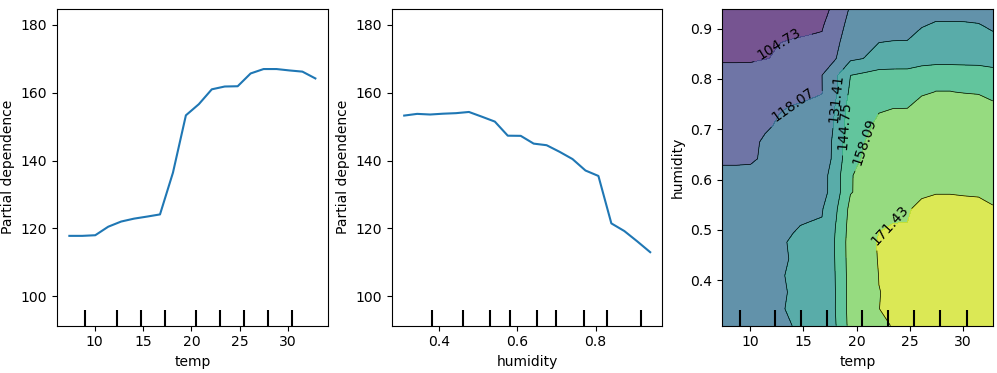
\includegraphics[width=0.8\textwidth]{chapters/linear/pics/partial_dependence.png}
    \caption{Пример PDP в задаче числа суточной аренды велосипедов.}
    \label{fig:pdp}
    \end{figure}

    \item \textbf{Влияние признаков (SHAP и LIME):} Современные методы, такие как SHAP (SHapley Additive exPlanations) и LIME (Local Interpretable Model-agnostic Explanations), позволяют объяснить предсказания модели для отдельных объектов.
\end{itemize}

\subsection*{Влияние мультиколлинеарности}
Мультиколлинеарность возникает, когда между признаками существует сильная корреляция. Это может приводить к нестабильным оценкам коэффициентов. Для её диагностики используют:
\begin{itemize}
    \item \textbf{Фактор инфляции дисперсии (VIF):}
    \[
    VIF_j = \frac{1}{1 - R_j^2},
    \]
    где $R_j^2$ --- коэффициент детерминации при регрессии $j$-го признака на остальные.

    \subsubsection{Коэффициент детерминации \( R^2 \)}

    Коэффициент детерминации (\( R^2 \)) — это метрика, используемая для оценки качества модели регрессии. Он показывает, какую долю дисперсии зависимой переменной (\( Y \)) модель способна объяснить.

    \subsubsection*{Формула}
    Коэффициент \( R^2 \) рассчитывается следующим образом:
    \[
    R^2 = 1 - \frac{SS_{\text{res}}}{SS_{\text{tot}}},
    \]
    где:
    \begin{itemize}
    \item \( SS_{\text{res}} = \sum_{i=1}^n (y_i - \hat{y}_i)^2 \) — остаточная сумма квадратов (сумма квадратов отклонений между реальными значениями \( y_i \) и предсказанными значениями \( \hat{y}_i \));
    \item \( SS_{\text{tot}} = \sum_{i=1}^n (y_i - \bar{y})^2 \) — общая сумма квадратов (сумма квадратов отклонений реальных значений \( y_i \) от среднего значения \( \bar{y} \));
    \item \( \bar{y} \) — среднее значение зависимой переменной:
    \[
    \bar{y} = \frac{1}{n} \sum_{i=1}^n y_i.
    \]
\end{itemize}

\subsection*{Интерпретация}
Значение \( R^2 \) находится в диапазоне от 0 до 1:
\begin{itemize}
    \item \( R^2 = 1 \): модель идеально объясняет дисперсию данных.
    \item \( R^2 = 0 \): модель не объясняет дисперсию данных (эквивалентно случайному предсказанию среднего значения \( \bar{y} \)).
    \item \( R^2 < 0 \): модель объясняет дисперсию хуже, чем случайное предсказание среднего значения.
\end{itemize}

Для задачи определения значимого признака, каждый признак по очереди берется в качестве независимой переменной и для каждого формулируется задача регрессии:

\begin{align}
X_{j} = \beta_0 + \sum_{i \neq j}^n\beta_{i} * X_{i}
\end{align}

Таким образом высокое значение VIF для отдельной переменной говорит об ее избыточности в обучаемой выборке, т.к. информация о ней (для линейной модели) почти полностью содержится в других признаках. На практике при значениях VIF > 10 говорят о мультиколениарности данных и избавляются от таких признаков или применяют L1, L2 регуляризации.

\subsection*{Практические примеры}
Рассмотрим несколько примеров использования линейных методов для интерпретации:
\begin{itemize}
    \item \textbf{Прогнозирование цен на недвижимость:} Вклад признаков, таких как площадь, расположение и возраст здания, можно интерпретировать напрямую через коэффициенты линейной модели.
    \item \textbf{Медицинская диагностика:} В задачах прогнозирования риска заболеваний линейные модели позволяют определить, какие факторы (например, возраст, уровень холестерина) оказывают наибольшее влияние.
\end{itemize}

\subsection*{Задачa 1: Доверительный интервал \(\beta_1\).}

Требуется найти доверительный интервал для \(\beta_1\), используя точки из этой главы.

\textbf{Решение:}

Для коэффициентов линейной регрессии используем формулы метода наименьших квадратов:
\begin{align*}
\beta_1 &= \frac{\sum_{i=1}^n (x_i - \bar{x})(y_i - \bar{y})}{\sum_{i=1}^n (x_i - \bar{x})^2}, \\
\beta_0 &= \bar{y} - \beta_1 \bar{x},
\end{align*}
где \(\bar{x}\) и \(\bar{y}\) — средние значения \(x\) и \(y\) соответственно.

Подставляя значения:
\begin{align*}
\bar{x} &= 3, \quad \bar{y} = 5.6, \\
\beta_1 &= \frac{\sum (x_i - 3)(y_i - 5.6)}{\sum (x_i - 3)^2} = 2.2, \quad \beta_0 = 5.6 - 2.2 \cdot 3 = -0.4.
\end{align*}

Средняя квадратная ошибка (MSE) определяется как:
\[
\text{MSE} = \frac{\sum_{i=1}^n (y_i - \hat{y}_i)^2}{n - 2},
\]
где \(\hat{y}_i\) — предсказанное значение для \(y_i\). Подставляя значения:
\[
\text{MSE} = \frac{(2 - 1.8)^2 + (3 - 3.6)^2 + (5 - 5.8)^2 + (7 - 8)^2 + (11 - 10.2)^2}{5 - 2} = 0.76.
\]

Стандартная ошибка для \(\beta_1\):
\[
\text{SE}(\beta_1) = \sqrt{\frac{\text{MSE}}{\sum_{i=1}^n (x_i - \bar{x})^2}} = \sqrt{\frac{0.76}{10}} = 0.275.
\]

Квантиль распределения Стьюдента для уровня доверия 95\% и \(n-2=3\) степеней свободы:
\[
t_{0.025, 3} \approx 3.182.
\]

Границы доверительного интервала:
\begin{align*}
CI_{\text{lower}} &= \beta_1 - t \cdot \text{SE}(\beta_1) = 2.2 - 3.182 \cdot 0.275 \approx 1.32, \\
CI_{\text{upper}} &= \beta_1 + t \cdot \text{SE}(\beta_1) = 2.2 + 3.182 \cdot 0.275 \approx 3.08.
\end{align*}

\textbf{Иллюстрация:}
На рисунке показана линия регрессии (красная), а также линии, соответствующие границам доверительного интервала (зелёная и оранжевая).

\begin{figure}[h!]
    \centering
    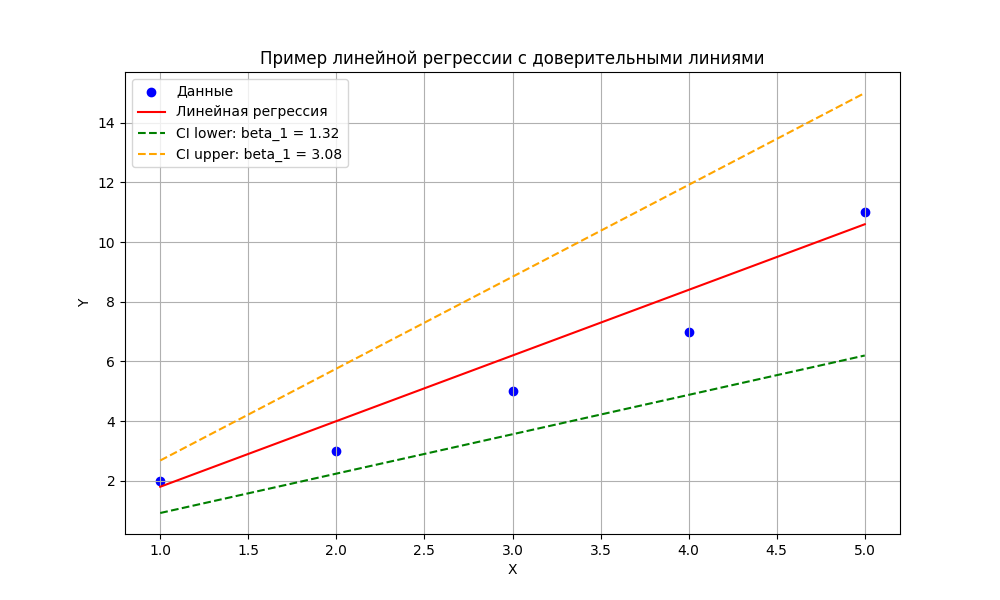
\includegraphics[width=0.8\textwidth]{chapters/linear/pics/beta_range.png}
    \caption{Пример линейной регрессии с доверительными интервалами.}
\end{figure}

\subsection*{Задача 2: Интерпретация PDP.}

Глядя на \ref{fig:pdp}, проведите анализ значимости изображенных признаков - температуры и влажности воздуха на общее количество арендуемых в день велосипедов. Какое влияние оказывают эти признаки на предсказываемую велечину? \\

\textbf{Решение:}

\begin{itemize}
 \item \textbf{Температура} оказывает значительное положительное влияние на предсказываемую величину, особенно в диапазоне 20-30 градусов
 \item \textbf{Влажность} оказывает отрицательное влияние: по мере её увеличения предсказания снижаются.
 \item \textbf{Совместное влияние} показало, что оптимальная комбинация — высокая температура и низкая влажность.
\end{itemize}

Оба эти признака являются значимыми для построения предсказательной модели, т.к. линии графиков PD имеют крутой наклон. Также видно что наклон на графике не постоянный и целесообразно задуматься об использовании нелинейной регресии или градиентного бустинга. \\\\

\subsection*{Задача 3: Определение мультиколениарности переменных по VIF.}

Сделать вывод о значимости переменных \(X_{2}\) и \(X_{3}\) \\

\begin{table}[h!]
\centering
\caption{Тренировочная выборка}
\begin{tabular}{|c|c|c|c|}
\hline
\textbf{\(Y\)} & \textbf{\( X_1 \)} & \textbf{\( X_2 \)} & \textbf{\( X_3 \)} \\ \hline
1                  & 1                  & 2                  & 3                  \\ \hline
2                  & 2                  & 4                  & 6                  \\ \hline
3                  & 3                  & 6                  & 9                  \\ \hline
4                  & 4                  & 8                  & 12                 \\ \hline
5                  & 5                  & 10                 & 15                 \\ \hline
\end{tabular}
\label{tab:example_vif}
\end{table}

\textbf{Решение:}

Не трудно видеть что:

\begin{align}
X_{2} = 2*X_{1} \text{\space\space} X_{3} = 3*X_{1}
\end{align}

Таким образом оба этих признака линейно зависимы и никакой информации в себе не несут. При использовании формул для VIF, можно также убедится

\begin{align}
VIF_{2} -> \infty \text{\space\space} VIF_{3}-> \infty
\end{align}
\section{Многоклассовая классификация}

Задача многоклассовой классификации решает проблему нахождения принадлежности объекта к одному из $K$ классов: $Y = \{1, 2, ..., K\}$. В этом разделе будут разобраны некоторые из самых популярных подходов: one-vs-all, all-vs-all и многоклассовая логистическая регрессия. В качестве примера возьмем датасет из \href{https://education.yandex.ru/handbook/ml/article/linear-models}{хендбука Яндекса}, продемонстрированный на Рис. \ref{fig:linear-multi-dataset}.

\begin{figure}[ht]
	\centering
	\includegraphics[width=0.8\linewidth]{chapters/linear/pics/multi-dataset.png}
	\caption{Пример датасета задачи многоклассовой классификации}
	\label{fig:linear-multi-dataset}
\end{figure}

\subsection{Один против всех (one-versus-all)}

Обучим $K$ линейных классификаторов $b_1(x),...,b_K(x)$, выдающих оценки принадлежности классам $1,...,K$ соответственно. В случае с линейными моделями эти классификаторы будут иметь вид $b_k(x) = \operatorname{sign}(\langle w_k, x \rangle+w_{0k})$

Классификатор с номером $k$ будем обучать по выборке $(x_i, 2 \mathbb{I}[y_i = k] -1)^\ell_{i=1} $; иными словами, мы учим классификатор отличать $k$-й класс от всех остальных.

Логично, чтобы итоговый классификатор выдавал класс, соответствующий самому уверенному из бинарных алгоритмов. Уверенность можно в каком-то смысле измерить с помощью значений линейных функций:

$ a(x)= \operatorname{arg}\max\limits_{k \in Y} (\langle w_k, x \rangle+w_{0k})$

Давайте посмотрим, что даст этот подход применительно к нашему датасету. Обучим три линейных модели, отличающих один класс от остальных (Рис. \ref{fig:linear-multi-ova-models}).

\begin{figure}[H]
	\centering
	\includegraphics[width=0.8\linewidth]{chapters/linear/pics/multi-ova-models.png}
	\caption{Каждая из трех моделей, отделяющие свои классы}
	\label{fig:linear-multi-ova-models}
\end{figure}

Теперь сравним значения линейных функций на Рис. \ref{fig:linear-multi-ova-values}.

\begin{figure}[H]
	\centering
	\includegraphics[width=0.8\linewidth]{chapters/linear/pics/multi-ova-values.png}
	\caption{Значения функций моделей}
	\label{fig:linear-multi-ova-values}
\end{figure}

и для каждой точки выберем тот класс, которому соответствует большее значение, то есть самый «уверенный» классификатор, и изобразим это на Рис. \ref{fig:linear-multi-ova-final}

\begin{figure}[H]
	\centering
	\includegraphics[width=0.8\linewidth]{chapters/linear/pics/multi-ova-final.png}
	\caption{Итог разделения пространства на классы}
	\label{fig:linear-multi-ova-final}
\end{figure}

Хочется сказать, что самый маленький класс «обидели».

Проблема данного подхода заключается в том, что каждый из классификаторов $b_1(x),...,b_K(x)$ обучается на своей выборке, и значения линейных функций $\langle w_k, x \rangle+w_{0k}$ или, проще говоря, "выходы" классификаторов могут иметь разные масштабы. Из-за этого сравнивать их будет неправильно. Нормировать вектора весов, чтобы они выдавали ответы в одной и той же шкале, не всегда может быть разумным решением: так, в случае с SVM веса перестанут являться решением задачи, поскольку нормировка изменит норму весов.

\subsection*{Задача}

Подумайте, какой простой двумерный датасет особенно плохо работает с данным подходом с линейным классификатором (что вызвано исключительно характером распределения классов, а не выбросами, количеством данных и т.п.).

\subsection*{Ответ}

Примером такого датасета могут послужить три класса, такие что один находится между двумя другими, как на Рис. \ref{fig:linear-multi-ova-contrprimer}. В этом случае нельзя полагаться на значения разделяющей функции, так как, например, зеленый класс лежит сильно дальше границы желтого и синего классов, чем сам желтый класс. Поэтому, желто-синий классификатор будет относить зеленые точки к желтому цвету с большей уверенностью, чем желтые.

\begin{figure}[H]
	\centering
	\includegraphics[width=0.8\linewidth]{chapters/linear/pics/multi-ova-contrprimer.png}
	\caption{Контрпример к one-vs-all}
	\label{fig:linear-multi-ova-contrprimer}
\end{figure}

\subsection{Все против всех (all-versus-all)}

Обучим  $C^2_k$ классификаторов $a_{ij}(x), i, j = 1,..,K, i \neq j$. Например, в случае с линейными моделями эти модели будут иметь вид

$a_{ij}(x) = \operatorname{sign}(\langle w_{ij}, x \rangle+w_{0,ij})$

Классификатор $a_{ij}(x)$ будем настраивать по подвыборке $X_{ij} \subset X$, содержащей только объекты классов $i$ и $j$. Соответственно, классификатор $a_{ij}(x)$ будет выдавать для любого объекта либо класс $i$, либо класс $j$. Проиллюстрируем это для нашей выборки на Рис. \ref{fig:linear-multi-ava-models}

\begin{figure}[H]
	\centering
	\includegraphics[width=0.8\linewidth]{chapters/linear/pics/multi-ava-models.png}
	\caption{Классификаторы, разделяющие по два класса}
	\label{fig:linear-multi-ava-models}
\end{figure}

Чтобы классифицировать новый объект, подадим его на вход каждого из построенных бинарных классификаторов. Каждый из них проголосует за свой класс; в качестве ответа выберем тот класс, за который наберется больше всего голосов:

$a(x) = \operatorname{arg}\max\limits_{k \in Y} \sum\limits_{i=1}^K\sum\limits_{j\neq i} \mathbb{I}[a_{ij}(x) = k]$

Для нашего датасета получается следующая картинка на Рис. \ref{fig:linear-multi-ava-final}

\begin{figure}[H]
	\centering
	\includegraphics[width=0.8\linewidth]{chapters/linear/pics/multi-ava-final.png}
	\caption{Итоговый результат для all-vs-all}
	\label{fig:linear-multi-ava-final}
\end{figure}

Обратите внимание на серый треугольник на стыке областей. Это точки, для которых голоса разделились (в данном случае каждый классификатор выдал какой-то свой класс, то есть у каждого класса было по одному голосу). Для этих точек нет явного способа выдать обоснованное предсказание.

\subsection{Многоклассовая логистическая регрессия}

Некоторые методы бинарной классификации можно напрямую обобщить на случай многих классов. Выясним, как это можно проделать с логистической регрессией.

В логистической регрессии для двух классов мы строили линейную модель

$b(x) = \langle w, x \rangle+w_0$

а затем переводили её прогноз в вероятность с помощью сигмоидной функции $\sigma(M) = \frac{1}{1+\operatorname{exp}(-M)}$. Допустим, что мы теперь решаем многоклассовую задачу и построили $K$ линейных моделей

$b_k(x) = \langle w_k, x \rangle+w_{0k}$

каждая из которых даёт оценку принадлежности объекта одному из классов. Как преобразовать вектор оценок $(b_1(x),...,b_K(x))$ в вероятности? Для этого можно воспользоваться оператором $\operatorname{softmax}(z_1,...,z_k)$,

\subsection*{Задача}

Подумайте, как должен выглядеть этот оператор, зная, что в случае двух классов он совпадает с сигмоидой, принимает значения от нуля до единицы и равен вектору вероятностей принадлежности каждому из классов.

\subsection*{Ответ}

$\operatorname{softmax}(z_1,...,z_k) = \left( \frac{\exp{(z_1)}}{\sum^K_{k=1}\exp{(z_k)}}, ..., \frac{\exp{(z_K)}}{\sum^K_{k=1}\exp{(z_k)}}, \right)$ \newline

В этом случае вероятность $k$-го класса будет выражаться как

$P(y=k|x,w) = \frac{\exp{(\langle w_k, x \rangle+w_{0k})}}{\sum^K_{j=1}\exp{(\langle w_j, x \rangle+w_{0j})}}$

Обучать эти веса предлагается с помощью метода максимального правдоподобия: так же, как и в случае с двухклассовой логистической регрессией:

$\sum\limits_{i=1}^\ell \log P(y=y_i|x_i,w) \xrightarrow{} \max\limits_{w_1,...,w_K}$

\subsection*{Задача}

Подумайте, какой существует простой многоклассовый (нелинейный) классификатор, использующий только расстояние между объектами и не требующий обучения (у него отсутствуют параметры, есть только гиперпараметр).

\subsection*{Ответ}

Таким классификатором является KNN, или метод $k$ ближайших соседей. Этот алгоритм причисляет объект к самому популярному классу среду его $k$ ближайших соседей.

\section{Логистиеская регрессия}
\subsection*{Что такое логистическая регрессия?}

Логистическая регрессия — это статистический метод, используемый для классификации объектов на два или более классов. Она применяется, когда целевая переменная (\(y\)) принимает дискретные значения, чаще всего \(y \in \{0, 1\}\). Основной задачей логистической регрессии является предсказание вероятности принадлежности объекта к определённому классу.
 Примеры таких задач: Классификация писем на спам и не спам, предсказание вероятности заболевания на основе медицинских данных, прогноз поступления студента на основе экзаменационных баллов.

\subsection*{Идея логистической регрессии}

Логистическая регрессия основывается на линейной регрессии, но с одной важной модификацией: вместо того, чтобы предсказывать значения на бесконечном числовом отрезке, она ограничивает прогнозируемые значения интервалом \([0, 1]\). Это достигается с помощью логистической функции, которая преобразует линейное выражение в вероятность.


\subsection*{Математическая формулировка}


Сначала вычисляется линейная комбинация входных признаков:
\[
z = b_0 + b_1x_1 + b_2x_2 + \dots + b_nx_n,
\]
где:
- \(b_0\) — свободный член (интерсепт),
- \(b_1, b_2, \dots, b_n\) — коэффициенты модели,
- \(x_1, x_2, \dots, x_n\) — входные признаки.


Логистическая функция (или сигмоида) преобразует \(z\) в значение вероятности \(P(y=1)\):
\[
P(y = 1) = \frac{1}{1 + e^{-z}} = \sigma(z)
\]

\begin{figure}[H]
	\centering
	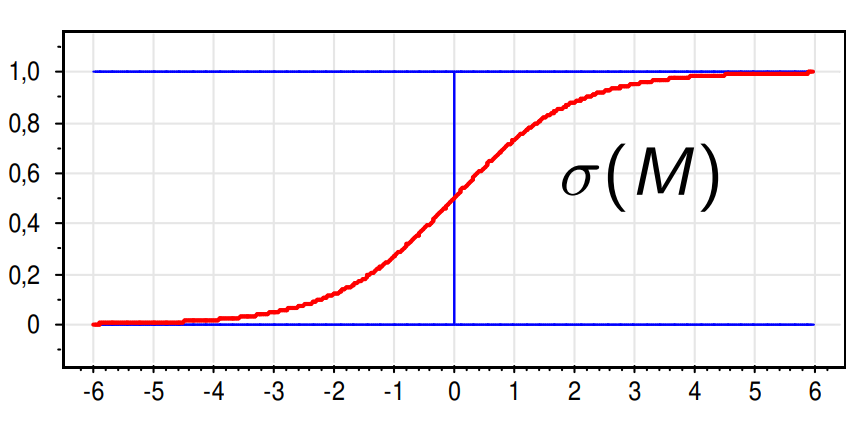
\includegraphics[width=0.8\linewidth]{chapters/linear/pics/sigmoida.png}
	\caption{График сигмоидной функции}
	\label{fig:sigmoida}
\end{figure}
Вероятность принадлежности к классу \(y=0\) вычисляется как:
\[
P(y = 0) = 1 - P(y = 1).
\]


Если вероятность \(P(y=1) \geq 0.5\), объект относят к классу \(y=1\); иначе — к классу \(y=0\).


Чтобы упростить обучение модели, применяется логарифмическая трансформация. Логарифмические шансы (логиты) определяются как:
\[
\text{logit}(P) = \ln\left(\frac{P(y = 1)}{1 - P(y = 1)}\right).
\]

Так как \(P(y = 1) = \frac{1}{1 + e^{-z}}\), подставим:
\[
\ln\left(\frac{P(y = 1)}{1 - P(y = 1)}\right) = z = b_0 + b_1x_1 + \dots + b_nx_n.
\]

\subsection*{Обучение логистической регрессии}

1. Функция правдоподобия

Вероятность \(P(y)\) для одного наблюдения записывается как:
\[
P(y) = P(y = 1)^{y} \cdot (1 - P(y = 1))^{1 - y}.
\]

Для всех наблюдений функция правдоподобия равна произведению вероятностей:
\[
L(\mathbf{b}) = \prod_{i=1}^m P(y_i | x_i).
\]

2. Логарифм правдоподобия

Чтобы упростить вычисления, берётся логарифм функции правдоподобия:
\[
\ell(\mathbf{b}) = \sum_{i=1}^m \left[y_i \ln(P(y_i)) + (1 - y_i) \ln(1 - P(y_i))\right].
\]

3. Максимизация логарифма правдоподобия

Коэффициенты \(\mathbf{b} = [b_0, b_1, \dots, b_n]\) определяются так, чтобы логарифм правдоподобия был максимален. Это достигается методами оптимизации, например, градиентным спуском.


\subsection*{Задача 1: Голосование на выборах}

\textbf{Условие:}  
Политическая партия пытается спрогнозировать, проголосует ли человек за неё, исходя из возраста \(x_1\) и политической активности \(x_2\) (в часах участия в митингах за год).  
Известны данные:  
\[
\begin{aligned}
    &\text{Человек 1: } x_1 = 22, x_2 = 15, \text{ проголосовал (}\, y = 1). \\
    &\text{Человек 2: } x_1 = 45, x_2 = 2, \text{ не проголосовал (}\, y = 0). \\
    &\text{Человек 3: } x_1 = 30, x_2 = 10, \text{ проголосовал (}\, y = 1).
\end{aligned}
\]

Определите, проголосует ли человек с \(x_1 = 35\) и \(x_2 = 8\). Используйте коэффициенты \(b_0 = -8\), \(b_1 = 0.2\), \(b_2 = 0.5\).  

\textbf{Решение:}

1. Записываем логистическую функцию:  
\[
P(y = 1) = \frac{1}{1 + e^{-(b_0 + b_1x_1 + b_2x_2)}}.
\]



2. Подставляем значения \(x_1 = 35\), \(x_2 = 8\):  
\[
z = b_0 + b_1x_1 + b_2x_2 = -8 + 0.2 \cdot 35 + 0.5 \cdot 8 = -8 + 7 + 4 = 3.
\]

3. Вычисляем вероятность:  
\[
P(y = 1) = \frac{1}{1 + e^{-3}} \approx 0.9526.
\]

4. Так как \(P(y = 1) > 0.5\), человек проголосует.  
Ответ: проголосует.


\subsection*{Задача 2: Магазин}

\textbf{Условие:}  
Магазин оценивает вероятность покупки товара клиентом в зависимости от времени, которое клиент проводит на сайте. Для этого применяется логистическая регрессия. Её уравнение:
\[
P(y = 1) = \frac{1}{1 + e^{-(b_0 + b_1x_1)}}.
\]

Где x - время проведённое на сайте в минутах, b_0 = -1.5, b_1 = 0.7


Какова вероятность того, что клиент, проведший 3 минуты на сайте, сделает покупку?

\textbf{Решение:}  

1. Записываем логистическую функцию:  
\[
P(y = 1) = \frac{1}{1 + e^{-(b_0 + b_1x_1)}}.
\]

3. Подставляем значения \(b_0 = -1.5\), \(b_1 = 0.7\):  
\[
z = b_0 + b_1x_1 = -1.5 + 2.1 = 0.6
\]

4. Вычисляем вероятность:  
\[
P(y = 1) = \frac{1}{1 + e^{-0.6}} \approx 0.645
\]

Ответ: 64.5\%


\subsection*{Задача 3: Утечка газа}

\textbf{Условие:}  
На химическом заводе нужно спрогнозировать, есть ли утечка газа в системе на основе двух факторов:  
- \(x_1\): температура трубы (в градусах);  
- \(x_2\): давление внутри трубы (в барах).  

Известные данные:  
\[
\begin{aligned}
    &\text{Ситуация 1: } x_1 = 500, x_2 = 100, \text{ утечка (}\, y = 1). \\
    &\text{Ситуация 2: } x_1 = 300, x_2 = 80, \text{ нет утечки (}\, y = 0). \\
    &\text{Ситуация 3: } x_1 = 400, x_2 = 90, \text{ утечка (}\, y = 1).
\end{aligned}
\]

Определите, будет ли утечка при \(x_1 = 450\) и \(x_2 = 85\). Используйте коэффициенты \(b_0 = -30\), \(b_1 = 0.05\), \(b_2 = 0.1\).

\textbf{Решение:}  

1. Записываем логистическую функцию:  
\[
P(y = 1) = \frac{1}{1 + e^{-(b_0 + b_1x_1 + b_2x_2)}}.
\]

2. Подставляем значения \(x_1 = 450\), \(x_2 = 85\):  
\[
z = b_0 + b_1x_1 + b_2x_2 = -30 + 0.05 \cdot 450 + 0.1 \cdot 85 = -30 + 22.5 + 8.5 = 1.
\]

3. Вычисляем вероятность:  
\[
P(y = 1) = \frac{1}{1 + e^{-1}} \approx 0.731.
\]

4. Так как \(P(y = 1) > 0.5\), утечка будет.  
Ответ: утечка будет.

\section{Алгоритмы Passive-Aggressive (PA) в линейной классификации}
\subsection*{Базовые сведения.}

Алгоритмы Passive-Aggressive (PA) являются онлайн-алгоритмами для обучения линейных моделей классификации.
Эти алгоритмы предназначены для обработки данных в режиме реального времени, где модель обновляется по мере поступления новых данных. PA-алгоритмы широко используются в задачах, где данные поступают последовательно, и требуется быстро адаптироваться к новой информации.

\subsection*{Классификафия PA алгоритмов}

PA-алгоритмы балансируют между "пассивным" и "агрессивным" обновлением весов модели:

PA-I (Passive-Aggressive I): Обновляет веса только в случае ошибочной классификации, используя минимальное изменение весов для исправления ошибки.

PA-II (Passive-Aggressive II): Всегда обновляет веса, но размер обновления зависит от правильности классификации и параметра регуляризации C.

\subsection*{Математическая формулировка}

Для PA-I, Если $y_t(w_t \cdot x_t) < 1$, $\eta = \frac{1 - y_t(w_t \cdot x_t)}{||x_t||^2}$

\[
    w_{t+1} = w_t + \eta y_t x_t
\]


Для PA-II
\[
\eta = \frac{1 - y_t(w_t \cdot x_t)}{C||x_t||^2 + ||x_t||^2}
\]

\[
    w_{t+1} = w_t + \eta y_t x_t
\]


\subsection*{Шаги алгоритма}

1) Инициализация: Начальная инициализация весов модели (обычно нулевой вектор).

2) Обработка каждого примера:

Получить входной вектор $x$ и метку $y$ $(y \in \{−1,+1\})$.

Вычислить предсказание: $y_{\text{pred}} = \sign (w^T x)$

Если $y_{\text{pred}} \ne y$, произошла ошибка, обновить веса согласно PA-I или PA-II.

3) Завершение: После обработки всех примеров модель готова к использованию для классификации новых данных.

\subsection*{Применения PA}

Текстовая классификация: PA-алгоритмы хорошо подходят для задач классификации текстов, таких как спам-фильтрация и анализ sentiment.

Рекомендательные системы: Используются для рекомендации товаров, фильмов и музыки.

Обработка потоковых данных: Эффективны в обработке данных в реальном времени, например, в анализе социальных сетей и торговых данных.


\subsection*{Задача 1: Обновление весов в PA-I}

\textbf{Условие:}  

Начальные веса модели $w = (0, 0)$

Входной вектор $x = (1, 2)$

Метка $y = 1$

Предсказание было ошибочным.

\textbf{Решение:}

1. Вычислим скалярное произведение:
\[
    w \cdot x = 0 \cross 1 + 0 \cross 2 = 0
\]


2. Вычислим $y \cross (w \cdot x)$
\[
y \cross (w \cdot x) = 1 \cross 0 = 0
\]

3. Вычислим $\eta$:

\[
    \eta = \frac{1 - y\cross(w \cdot x)}{||x||^2} = \frac{1 - 0}{1^2 + 2^2} = \frac{1}{5} = 0.2
\]

4. Обновим веса

\[
    w_{\text{new}} = w + \eta \cross y \cross x = (0, 0) + 0.2 \cross 1 \cross (1, 2)  = (0.2, 0.4)
\]

\subsection*{Задача 2: Обновление весов в PA-II}

\textbf{Условие:}

Начальные веса модели $w = (1, -1)$

Входной вектор $x = (2, 1)$

Метка $y = -1$

Параметр регуляризации $C = 0.5$

Предсказание ошибочным.


\textbf{Решение:}

1. Вычислим скалярное произведение:
\[
    w \cdot x = 1 \cross 2 + (-1) \cross 1 = 2 - 1 = 1
\]


2. Вычислим $y \cross (w \cdot x)$
\[
    y \cross (w \cdot x) = (-1) \cross 1 = -1
\]


3. Вычислим \eta
\[
    \eta = \frac{1 - y\cross(w \cdot x)}{C||x||^2 + ||x||^2} = \frac{1 - (-1)}{0.5 \cross (2^2 + 1^2)} = \frac{2}{0.5 \cross 5 + 5} = \frac{2}{7.5} \eqiv 0.26
\]

4. Обновим веса

\[
    w_{\text{new}} = w + \eta \cross y \cross x = (1, -1) + 0.26 \cross (-1) \cross (1, 1)  = (1 - 0.53, -1 - 0.26) = (0.46, -1,26)
\]

\subsection*{Задача 3: Сравнение PA-I и PA-II}

\textbf{Условие:}  
Сравните алгоритмы PA-I и PA-II в терминах обновления весов при правильной и ошибочной классификации. В каких случаях PA-II может быть предпочтительнее PA-I и наоборот? Объясните, используя математические формулы и примеры.
\textbf{Решение:}  
PA-I (Passive-Aggressive I):

Обновляет веса только в случае ошибки классификации.
Использует минимальное изменение весов для исправления ошибки.

\[
    \eta = \frac{1 - y_t\cross(w_t \cdot x_t)}{||x_t||^2}
\]

Если  $y \cross (w \cdot x) \ge 1$, обновление не происходит (пассивное поведение).

Если  $y \cross (w \cdot x) < 1$, обновление не происходит (агрессивное поведение).

PA-I предпочтительнее в случаях, когда нужно минимизировать обновления и поддерживать стабильность модели, если ошибок нет.


Не обновляет веса, если предсказание правильное, это позволяет PA-II постепенно адаптироваться к новым данным, даже если предсказание было правильным


PA-II (Passive-Aggressive II):
Всегда обновляет веса, но размер обновления зависит от уверенности предсказания.


\[
\eta = \frac{1 - y_t(w_t \cdot x_t)}{C||x_t||^2 + ||x_t||^2}
\]

Где $C$ - параметр регуляризации, который контролирует "агрессивность" обновления.


Обновляет веса даже при правильной классификации, но с небольшим шагом ($\eta$ мало).
Это позволяет PA-II постепенно адаптироваться к новым данным, даже если предсказание было правильным.

\section*{Обобщённые линейные модели (GLM)}

Обобщённые линейные модели расширяют линейную регрессию для оперирования целевыми переменными, которые обладают различными распределениями. Такие модели состоят из трёх компонентов:
\begin{itemize}
    \item Систематической части: линейного предсказателя $\eta = X\beta$, где $X$ — это матрица признаков, а $\beta$ — вектор коэффициентов.
    \item Случайной части: распределение выборки, например нормальное, Пуассоновское, биномиальное и т.д.
    \item Функции связи $g(\cdot)$: увязывает средний ответ $E[Y]$ с линейным предсказателем $\eta$ через $g(E[Y]) = \eta$.
\end{itemize}

\section*{Функции связи}

Функции связи преобразуют линейную комбинацию объясняющих переменных в шкалу, которая уместна для распределения отклика. Ниже описаны несколько популярных функций связи:

\subsection*{Логистическая функция связи}

Используется в логистической регрессии для двоичных классификаций. Функция логистической связи представлена следующим образом:
\[
g(\mu) = \log \left( \frac{\mu}{1-\mu} \right)
\]
где $\mu = E[Y]$ и $Y \sim \text{Bernoulli}(p)$.

\section*{Логистическая функция и сигмоида}

Логистическая функция связи часто представляется в виде сигмоидной функции \( \sigma(t) \), которая преобразует любое вещественное число в значение в диапазоне от 0 до 1:

\[
\sigma(t) = \frac{1}{1 + e^{-t}}
\]

где \( t = X\beta \), а \( X\beta \) — это линейный предсказатель, комбинация независимых переменных и их коэффициентов.

\section*{Применение в логистической регрессии}

Задача логистической регрессии заключается в оценке вероятности принадлежности объекта к одному из двух классов. Вероятность успешного исхода определяется как:

\[
P(Y=1 | X) = \sigma(X\beta) = \frac{1}{1 + e^{-(X\beta)}}
\]

Кроме того, вероятность принадлежности ко второму классу:

\[
P(Y=0 | X) = 1 - \sigma(X\beta)
\]

Таким образом, логистическая функция связи позволяет задействовать линейные модели в задачах нелинейной классификации.

\subsection*{Пробитная функция связи}

Пробитная связь применима как альтернатива логистической для задач бинарной классификации. Она определяется через обратную функцию нормального распределения:
\[
g(\mu) = \Phi^{-1}(\mu)
\]
где $\Phi^{-1}(\cdot)$ — обратная функция стандартного нормального распределения.

\section*{Сравнение с логистической функцией связи}

Пробитная и логистическая функции связи очень похожи и часто дают схожие результаты в задачах бинарной классификации. Следует отметить различие в функциональной форме: в пробитной регрессии используется нормальное распределение, в то время как в логистической — логистическое распределение.

\section*{Применение}

Пробитная функция связи находит применение в экономиках и финансах, особенно когда распределение ошибок предполагается нормальным. Она известна в анализе бинарных выборов, таких как покупательское поведение или инвестиционные решения.

\subsection*{Логарифмическая функция связи}

Часто используется в Пуассоновской регрессии и моделировании счётных данных:
\[
g(\mu) = \log(\mu)
\]
Подходит для моделирования данных, у которых средний уровень экспоненциально увеличивается.

\section*{Применение в моделях}

Логарифмическая функция связи часто используется в:

\begin{itemize}
    \item \textbf{Пуассоновской регрессии:} Моделирование частоты событий, которые происходят в фиксированное количество времени, например, количество звонков в колл-центр за час.
    \item \textbf{Гамма-регрессии:} Работает с положительными вещественными данными, такими как время до события или расходы.
\end{itemize}

В обобщённой линейной модели (GLM) с логарифмической функцией связи, линейный предсказатель \(X\beta\) связан с ожиданием зависимой переменной через:

\[
\log(\mu) = X\beta
\]

или, эквивалентно,

\[
\mu = e^{X\beta}
\]

\section*{Интерпретация и особенности}

Логарифмическая функция связи позволяет моделям учитывать экспоненциальные изменения в данных, что делает её мощным инструментом для анализа данных, в которых изменения варьируются в широком диапазоне.

\subsection*{Идентичная функция связи}

В линейной регрессии используется идентичная функция связи, что делает предсказание тождественным линейному предсказателю:
\[
g(\mu) = \mu
\]
\section*{Задача 1: Анализ страховых выплат}

\textbf{Сценарий:} 
Страховая компания анализирует данные о выплатах по страховым случаям. Необходимо понять, как разные зависимости признаков влияют на выплату. Имеется информация о возрастах клиентов, продолжительности страховки и числе страховых случаев.

\textbf{Вопрос:} 
Какая функция связи будет наиболее подходящей для моделирования положительных страховых выплат?

\textbf{Решение:} 
Для задачи прогнозирования средних положительных величин, как страховые выплаты, часто используется гамма-регрессия. Здесь логарифмическая функция связи будет уместной:
\[
g(\mu) = \log(\mu)
\]
Причина в том, что логарифмическая функция связи позволяет адекватно моделировать данные с ненормальным распределением, характеризующиеся только положительными значениями и результатами, зависящими от экспоненциального роста.

\section*{Задача 2: Классификация рисков клиентов}

\textbf{Сценарий:} 
Финансовая организация хочет классифицировать клиентов по вероятности неудачного возвращения кредита. Данные включают демографические характеристики, кредитную историю и текущие обязательства.

\textbf{Вопрос:} 
Какая функция связи наиболее подходит для логистической регрессии, применимой для двоичной классификации? Предположите, что выходные данные — вероятность неудачного погашения кредита.

\textbf{Решение:} 
Для задач, связанных с вероятностными предсказаниями, логистическая функция связи — лучший выбор:
\[
g(\mu) = \log \left( \frac{\mu}{1-\mu} \right)
\]
где $\mu = E[Y]$, отражает вероятность нахождения клиента в группе "рискованных". Логистическая функция переводит значения в диапазон от 0 до 1, который интерпретируется как вероятность принадлежности к классу.


    \clearpage
    \chapter{Основы нейросетевых моделей}
    \section{Полносвязная нейронная сеть (Персептрон).}

\subsection{Модель нейрона МакКаллока-Питтса}

Рассмотрим модель нейрона МакКаллока-Питтса (1943) \cite{ModelMcCullochPitts}. Множество объектов $X$ (количество элементов множества $M$), множество ответов $Y$ (количество элементов множества $H_L$). Признаки объектов задаются вектором функций $\overrightarrow{f(x)} = [f_1(x), f_2(x), \dots, f_n(x)]^T$ таких, что $f_j: X \rightarrow \mathbb{R}$. Для объекта $x_m \in X$ с помощью этих функций определяется вектор вещественных признаков $\overrightarrow{x_m} = [x_m^1, x_m^2, \dots, x_m^n]^T$, где $x_m^j = f_j (x_m)$. Нейрон вычисляет функцию активации $\sigma$ от линейной комбинации вектора признаков $\overrightarrow{x_m}$ с весами $\overrightarrow{w}$. То есть выход нейрона $a(\overrightarrow{x_m}, \overrightarrow{w})$ вычисляется по формуле:
$$
a(\overrightarrow{x_m}, \overrightarrow{w}) = \sigma(\sum_{i = 1}^{n} x_m^i w_i - w_0) = \sigma (<\overrightarrow{x_m}, \overrightarrow{w}>)
$$
Математическая модель нейрона изображена на рисунке \ref{img:McCullochPittsModel}. Функцией активации $\sigma$ может быть любая непрерывная нелинейная функция. Нелинейность функции нужна, чтобы иметь возможность приблизить любую непрерывную функцию с желаемой точностью (теорема Горбаня, 1998). В формуле вектор признаков $\overrightarrow{x_m}$ дополнен элементом $-1$, который имеет вес $w_0$, что соответствует физической интерпретации нейрона. Нейрон $m$ получает на вход множество электрических сигналов $x_m^i$ по дендритам $i$. Каждый дендрит $i$ имеет свою толщину, и соответственно проводимость $w_i$. Чем выше проводимость $w_i$, тем больший вклад сигнала с данного дендрита в общую сумму. Нейрон суммирует сигналы с дендритов и если сумма выше порогового значения $w_0$, то он передаёт информацию дальше по аксону. Сигнал на выходе нейрона, то есть аксоне, определяется функцией активации $\sigma$.

\begin{figure}[h]
	\centering
	\includegraphics[width=0.4\linewidth]{chapters/neural/images/neuron1.png}
	\caption{Математическое описание модели нейрона МакКаллока-Питтса.}
	\label{img:McCullochPittsModel}
\end{figure}

\subsection{Реализация логических функций с помощью нейрона}

Рассмотрим применение описанного выше нейрона для реализации простейших логических функций.

\textbf{Логическая функция <<и>>}. Обозначение $\wedge$. На вход поступают признаки $x^1, x^2$, результат функции $a = x^1 \wedge x^2$. Нейронной реализацией будет $a = [x^1 + x^2 - \frac{3}{2} > 0]$, где функция активации $[x > 0]$ равна 1, если $x > 0$, и равна 0 в противном случае.

\begin{figure}[h]
	\centering
	\subfloat[Таблица истинности функции <<и>>]{
		\centering
		\begin{tabular}{|c|c|c|}
			\hline
			$x^1$ & $x^2$ & $a = x^1 \wedge x^2$ \\
			\hline
			0 & 0 & 0 \\
			0 & 1 & 0 \\
			1 & 0 & 0 \\
			1 & 1 & 1 \\
			\hline
		\end{tabular}
	}
	\hfill
	\subfloat[Модель нейрона, описывающего функцию <<и>>]{
		\centering
		\includegraphics[width=0.45\linewidth]{chapters/neural/images/function_and.png}
	}
\end{figure}

\textbf{Логическая функция <<или>>}. Обозначение $\vee$. На вход поступают признаки $x^1, x^2$, результат функции $a = x^1 \vee x^2$. Нейронной реализацией будет $a = [x^1 + x^2 - \frac{1}{2} > 0]$, где функция активации $[x > 0]$ равна 1, если $x > 0$, и равна 0 в противном случае.

\begin{figure}[h]
	\centering
	\subfloat[Таблица истинности функции <<или>>]{
		\centering
		\begin{tabular}{|c|c|c|}
			\hline
			$x^1$ & $x^2$ & $a = x^1 \vee x^2$ \\
			\hline
			0 & 0 & 0 \\
			0 & 1 & 1 \\
			1 & 0 & 1 \\
			1 & 1 & 1 \\
			\hline
		\end{tabular}
	}
	\hfill
	\subfloat[Модель нейрона, описывающего функцию <<или>>]{
		\centering
		\includegraphics[width=0.45\linewidth]{chapters/neural/images/function_or.png}
	}
\end{figure}

\textbf{Задача 1.} Привести модель нейрона, описывающего логическую функцию <<не>> $\neg x^1$.

\textbf{Решение:}

$a = [-x^1 + 1/2 > 0]$

\newpage

\textbf{Логическая функция <<исключающее или>>}. Обозначение $\oplus$. Данная функция не реализуема с помощью одного нейрона. Но может быть реализована нейронной сетью $[n_1, n_2, n_3]$: $n_1 = (x^1 \vee x^2)$, $n_2 = (x^1 \wedge x^2)$, $n_3 = [n_1 - n_2 - \frac{1}{2} > 0]$.

\begin{figure}[h]
	\centering
	\subfloat[Таблица истинности функции <<исключающее или>>]{
		\centering
		\begin{tabular}{|c|c|c|}
			\hline
			$x^1$ & $x^2$ & $a = x^1 \oplus x^2$ \\
			\hline
			0 & 0 & 0 \\
			0 & 1 & 1 \\
			1 & 0 & 1 \\
			1 & 1 & 0 \\
			\hline
		\end{tabular}
	}
	\hfill
	\subfloat[Модель нейрона, описывающего функцию <<исключающее или>>]{
		\centering
		\includegraphics[width=0.45\linewidth]{chapters/neural/images/function_xor.png}
	}
\end{figure}

\textbf{Задача 2.} Привести модель нейронной сети, описывающей логическую функцию $f(x^1, x^2, x^3)$, заданную таблицей истинности: \\
\begin{figure}[h]
	\centering
	\begin{tabular}{|c|c|c|c|}
		\hline
		$x^1$ & $x^2$ & $x^3$ & $f(x^1, x^2, x^3)$ \\
		\hline
		0 & 0 & 0 & 0 \\
		0 & 0 & 1 & 1 \\
		0 & 1 & 0 & 0 \\
		0 & 1 & 1 & 0 \\
		
		1 & 0 & 0 & 1 \\
		1 & 0 & 1 & 1 \\
		1 & 1 & 0 & 0 \\
		1 & 1 & 1 & 1 \\
		\hline
	\end{tabular}
\end{figure}

\textbf{Решение:}

Используем ранее описанные нейроны <<и>> $\wedge$, <<или>> $\vee$, <<не>> $\neg$. Перепишем функцию, используя эти операции: $f = ((\neg x^1) \wedge ((\neg x^2) \wedge x^3)) \vee (x^1 \wedge ((\neg x^2) \vee x^3))$. Конструируем нейроны: $n_1 = \neg x^1$, $n_2 = \neg x^2$, $n_3 = n_2 \wedge x^3$, $n_4 = n_1 \wedge n_3$, $n_5 = n_2 \vee x^3$, $n_6 = x^1 \wedge n_5$, $n_7 = n_4 \vee n_6$. Итоговая многослойная нейронная сеть состоит из нейронов $n_1, n_2, \dots n_7$. Результат сети находится на выходе нейрона $n_7$.

\newpage

\subsection{Область применимости многослойных нейронных сетей}

Согласно \cite{VorontsovSite}
\begin{enumerate}
	\item Двухслойная сеть в ${0, 1}^n$ позволяет реализовать произвольную булеву функцию.
	
	\item Линейный нейрон в $\mathbb{R}^n$ отделяет полупространство признаков гиперплоскостью. Тогда двухслойная сеть позволяет отделить многогранную область, не обязательно выпуклую и связную.
	
	\item Согласно теоремы Горбаня (1998) с помощью линейных операций и одной нелинейной функции активации можно приблизить любую непрерывную функцию с любой желаемой точностью.
\end{enumerate}

\subsection{Полносвязная нейронная сеть}

Обобщением рассмотренной выше модели является полносвязная нейронная сеть (рис. \ref{img:full_net}). Сеть состоит из входного слоя (жёлтый цвет), скрытых слоёв (зелёный цвет), и выходного слоя (оранжевый цвет). Выход одного слоя, поступает на вход другого. Обозначим количество нейронов в слое $l$ за $H_l$, в каждом слое оно может быть разным, $l \in \{1, 2, \dots, L\}$. Всего $L$ слоёв. Вектор $x^l$ -- это выход $l$-ого слоя и вход $l+1$, если $l \neq L$, то есть $x^l$ -- не последний слой. $x^0$ -- это вход нейронной сети. Матрицы коэффициентов перехода между слоями обозначим за $W^l$. $W^l$ -- это матрица перехода между слоями $l-1$ и $l$.

\begin{figure}[h]
	\centering
	\includegraphics[width=0.6\linewidth]{chapters/neural/images/full_net.png}
	\caption{Полносвязная нейронная сеть.}
	\label{img:full_net}
\end{figure}

Задачей обучения нейронной сети является минимизация средних потерь на обучающей выборке $X$ ($|X| = M$):
$$
Q(\overrightarrow{W}, X) = \frac{1}{m} \sum\limits_{m = 1}^{M} \mathcal{L} (\overrightarrow{W}, x_m) \rightarrow \min_{\overrightarrow{W}}
$$

Пусть объект $x$ описывается вектором признаков $\overrightarrow{x} = [x_1, x_2, \dots, x_n]^T$. В задаче классификации множество ответов $Y$ состоит из $H_L$ элементов. Тогда последний слой нейронной сети $x^{L}$ должен содержать $H_L$ элементов. Нейронная сеть предсказывает ответ $k$, если на её выходе наблюдается вектор $x^L = [0, \dots 0, 1, 0, \dots 0]^T$, где единица стоит на $k$-ом месте. 

Функция потерь может быть, например, квадратичной. Для объекта $x$ функция потерь вычисляется по формуле $\mathcal{L} (\overrightarrow{W}^{(t)}, x) = \frac{1}{2} \sum\limits_{i = 1}^{H_L} (x^L_i ((\overrightarrow{W}^{(t)}, x) - y_i)^2$, где $\overrightarrow{y}$ -- вектор из всех нулей кроме единицы на месте порядкового правильного ответа из множества ответов.

Рассмотрим различные методы обучения полносвязной нейронной сети.

\subsection{Градиентный спуск}

\begin{enumerate}
	\item Выбираем какое-то начальное приближение вектора матриц перехода $\overrightarrow{W}^{(0)}$.
	
	\item Итерационный процесс:
		$$
		\overrightarrow{W}^{(t+1)} = \overrightarrow{W}^{(t)} - h \cdot \overrightarrow{\nabla} Q(\overrightarrow{W}^{(t)}, X)
		$$
		где $h$ -- градиентный шаг или темп обучения.
		
		Для рассмотренного ранее эмпирического риска:
		$$
		\overrightarrow{W}^{(t+1)} = \overrightarrow{W}^{(t)} - \frac{h}{m} \cdot \overrightarrow{\nabla} \sum\limits_{m = 1}^{M} \mathcal{L} (\overrightarrow{W}^{(t)}, x_m)
		$$
		
	\item Повторяем итерационный процесс, пока эмпирический риск $Q(\overrightarrow{W}^{(t)}, X)$ или вектор матриц перехода $\overrightarrow{W}$ не сойдутся. Критерий сходимости может быть абсолютным, то есть когда модуль разности значений на последовательных шагах итерационного процесса меньше какого-то значения $\varepsilon$. Например, для эмпирического риска:
	$$
	\left| Q^{(t + 1)} - Q^{(t)} \right| < \varepsilon
	$$
	Или может быть относительным, когда модуль отношения разности значений на последовательных шагах итерационного процесса к наименьшему, или наибольшему значению, или к первому меньше $\varepsilon$. Например, для эмпирического риска:
	$$
	\left| \frac{Q^{(t + 1)} - Q^{(t)}}{\min \{ Q^{(t + 1)}, Q^{(t)} \} } \right| < \varepsilon
	$$
	При этом для эмпирического риска и для вектора матриц перехода значение $\varepsilon$ может быть разным.
	
	Для вектора матриц перехода можно предложить следующий способ:
	$$
	\left|\left| \overrightarrow{W}^{(t+1)} - \overrightarrow{W}^{(t)} \right|\right|_1 = \sum\limits_{l = 1}^{L} \sum\limits_{m = 1}^{m_l} \sum\limits_{n = 1}^{n_l} |W^l_{mn}{}^{(t+1)} - W^l_{mn}{}^{(t)}|
	$$
	где вектор матрица перехода рассматривается как вектор всех её элементов, и применяется первая норма. Размерность матрицы $W^l$ равна $m_l \times n_l$. $W^l_{mn}{}^{(t)}$ -- это элемент в $m$-ой строке $n$-ого столбца матрицы перехода между слоями $l-1$ и $l$ на шаге $t$ итерационного процесса.
\end{enumerate}

Недостатком данного метода является низкая скорость сходимости. Для ускорения применяется метод стохастического градиентного спуска.

\subsection{Стохастический градиентный спуск}

В отличие от обычного градиентного спуска, в котором вектор матриц перехода изменяется пропорционально градиенту эмпирического риска для всех объектов, в стохастическом градиенте вектор матриц перехода изменяется пропорционально функции потерь для одного объекта.

Алгоритм стохастического градиента:

\begin{enumerate}
	\item Выбираем какое-то начальное приближение вектора матриц перехода $\overrightarrow{W}^{(0)}$. Вычисляем первое приближение эмпирического риска:
	$$
	Q^{(0)}(\overrightarrow{W}^{(0)}, X) = \frac{1}{m} \sum\limits_{m = 1}^{M} \mathcal{L} (\overrightarrow{W}^{(0)}, x_m)
	$$
	
	\item Итерационный процесс: \\
 	Выбираем какой-нибудь объект $x \in X$, например случайным образом или перебираем все элементы $X$ по порядку. Корректируем вектор матриц перехода:
	$$
	\overrightarrow{W}^{(t+1)} = \overrightarrow{W}^{(t)} - h \cdot \overrightarrow{\nabla} \mathcal{L} (\overrightarrow{W}^{(t)}, x)
	$$
	где $h$ -- темп обучения.
	
	Эмпирический риск оценивается по формуле:
	$$
	Q^{(t+1)}(\overrightarrow{W}^{(t+1)}, X) = \lambda \mathcal{L} (\overrightarrow{W}^{(t)}, x) + (1-\lambda)  Q^{(t)}(\overrightarrow{W}^{(t)}, X)
	$$
	где $\lambda$ -- темп забывания предыстории.
	
	Рассмотрим, откуда взялась эта оценка $Q^{(t+1)}$.
	
	Если $Q^{(t)}$ -- среднее арифметическое объектов $\varepsilon_i$, $i = 1, 2, \dots t$, то
	$$
	Q^{(t)} = \frac{1}{t} \varepsilon_t + \frac{1}{t} \varepsilon_{t-1} + \frac{1}{t} \varepsilon_{t-2} + \dots + \frac{1}{t} \varepsilon_{1}
	$$
	$$
	Q^{(t - 1)} = \frac{1}{t-1} \varepsilon_{t-1} + \frac{1}{t-1} \varepsilon_{t-2} + \dots + \frac{1}{t-1} \varepsilon_{1}
	$$
	$Q^{(t)}$ можно выразить через $Q^{(t-1)}$:
	$$
	Q^{(t)} = \frac{1}{t} \varepsilon_t + \frac{t-1}{t} Q^{(t-1)} = \frac{1}{t} \varepsilon_t + (1 - \frac{1}{t}) Q^{(t-1)}
	$$
	
	Если $Q^{(t)}$ -- экспоненциальное скользящее среднее с параметром $\lambda$, то
	$$
	Q^{(t)} = \lambda \varepsilon_t + \lambda (1-\lambda) \varepsilon_{t-1} + \lambda (1-\lambda)^2 \varepsilon_{t-2} + \dots + \lambda (1-\lambda)^{t-1} \varepsilon_{1}
	$$
	$$
	Q^{(t - 1)} = \lambda \varepsilon_{t-1} + \lambda (1-\lambda) \varepsilon_{t-2} + \lambda (1-\lambda)^2 \varepsilon_{t-3} + \dots + \lambda (1-\lambda)^{t-2} \varepsilon_{1}
	$$
	Или $Q^{(t)}$ через $Q^{(t-1)}$:
	$$
	Q^{(t)} = \lambda \varepsilon_t + (1 - \lambda) Q^{(t - 1)}
	$$
	
	Пусть теперь $\lambda \sim \frac{1}{t}$. Тогда $(1-\lambda)^{t-1} = (1 - \frac{1}{t})^{t-1}$. $\lim\limits_{t\rightarrow \infty} (1 - \frac{1}{t})^{t-1} = \frac{1}{e}$. По аналогии из радиотехники, где для экспоненциально убывающего сигнала характерное время затухания измеряется по уменьшению сигнала в $e$ раз, тогда характерное количество членов, когда происходит затухание / <<забывание>> предыдущей истории ряда равно $t$.
		
	\item Повторяем итерационный процесс, пока эмпирический риск $Q(\overrightarrow{W}^{(t)}, X)$ или вектор матриц перехода $\overrightarrow{W}$ не сойдутся.
\end{enumerate}

\subsection{Метод обратного распространения ошибок (BackProp).}

Для вычисления градиента функции потерь применяется метод обратного распространения ошибок. Для упрощения формулы индекс ${}^{(t)}$ будем опускать.
$$
\overrightarrow{\nabla} \mathcal{L} (\overrightarrow{W}, x) = \left[\frac{\partial}{\partial W^0}, \frac{\partial}{\partial W^\partial}, \dots, \frac{\partial}{\partial W^L}\right]^T \cdot \mathcal{L} (\overrightarrow{W}, x)
$$

Для рассмотренной ранее квадратичной функции потерь:
$$
\overrightarrow{\nabla} \mathcal{L} (\overrightarrow{W}, x) = \left[\frac{\partial}{\partial W^0}, \frac{\partial}{\partial W^\partial}, \dots, \frac{\partial}{\partial W^L}\right]^T \cdot \frac{1}{2} \sum\limits_{i = 1}^{H_L} (x^L_i ((\overrightarrow{W}, x) - y_i)
$$
То есть выход нейронной сети $\overrightarrow{x^L}$ является функцией от вектора матриц перехода $\overrightarrow{W}$.

Выведем формулу, по которой нейронная сеть вычисляет $\overrightarrow{x^L}$. На первом слое сети находится вектор $\overrightarrow{x^0}$, который через матрицу перехода $W^1$ и вектор функций активации $\overrightarrow{\sigma_1}$ преобразуется во вход второго слоя $x^1$:
$$
\overrightarrow{x^1} = \overrightarrow{\sigma_1} (W^1 \cdot \overrightarrow{x^0})
$$
Аналогично для последующих слоёв:
$$
\overrightarrow{x^2} = \overrightarrow{\sigma_2} (W^2 \cdot \overrightarrow{x^1}) = \overrightarrow{\sigma_2} (W^2 \cdot \overrightarrow{\sigma_1} (W^1 \cdot \overrightarrow{x^0}))
$$
$$
\overrightarrow{x^L} = \overrightarrow{\sigma_L}(W^L \cdot \overrightarrow{x^{L-1}}) = \overrightarrow{\sigma_L}(W^L \cdot \overrightarrow{\sigma_{L-1}} (W^{L-1} \cdot \overrightarrow{\sigma_{L-1}}( \dots ( W^2 \cdot \overrightarrow{\sigma_1} (W^1 \cdot \overrightarrow{x^0})) \dots ))
$$

Чтобы получить формулы для обратного распространения ошибок необходимо найти $\overrightarrow{\nabla} \mathcal{L}$, рассматривая $\overrightarrow{x^L}$ как функцию $\overrightarrow{x^L} (\overrightarrow{W})$.

\textbf{Задача 3.} Доказать рекуррентные формулы для метода обратного распространения ошибок в предположениях:
\begin{enumerate}
	\item Функция потерь квадратичная $\mathcal{L} (\overrightarrow{W}, x) = \frac{1}{2} \sum\limits_{i = 1}^{H_L} (x^L_i ((\overrightarrow{W}, x) - y_i)^2$.
	
	\item Первый нейрон в слое нейронной сети всегда -1, то есть $\forall i: x^i_0 = -1$. $H_l$ -- количество нейронов в слое $l$ без учёта нейрона -1. Тогда индекс первого нейрона в слое, не всегда равного -1, равен 1, а индекс последнего нейрона равен $H_l$.
	
	\item Вектор функций активации $\overrightarrow{\sigma^l}$ зависит от отступа $\overrightarrow{M^l}$: $\sigma^l_n = \sigma^l_n(M^l_n)$, где $M_n = \sum\limits_{m = 1}^{H_l} W^l_{nm} x^{l-1}_{m}$. $\overrightarrow{M^l} = W^l \overrightarrow{x^{l-1}}$.
\end{enumerate}
$
\frac{\partial \mathcal{L}}{\partial x^L_n} = x^L_n - y_n
$, \\
$
\frac{\partial \mathcal{L}}{\partial W^L_{nm}} = \frac{\partial \mathcal{L}}{\partial x^L_n} \frac{\partial \sigma^L_n}{\partial M^L_n} x^{L-1}_{m}
$, \\
$
\frac{\partial \mathcal{L}}{\partial x^{l}_n} = \sum\limits_{m = 1}^{H_l} \frac{\partial \mathcal{L}}{\partial x^{l+1}_m} \frac{\partial \sigma^{l+1}_m}{\partial M^{l+1}_m} W^{l+1}_{mn}
$, \\
$
\frac{\partial \mathcal{L}}{\partial W^{l}_{nm}} = \frac{\partial \mathcal{L}}{\partial x^{l}_n} \frac{\partial \sigma^{l}_n}{\partial M^{l}_n} x^{l-1}_{m}
$, \\
$1 \le l < L$.

\textbf{Решение:}

Сначала докажем соотношения для $l = L$.

Рассматриваем функцию потерь как сложную функцию $\mathcal{L} (\overrightarrow{W}) = \mathcal{L}(\overrightarrow{x^L}(\overrightarrow{W}))$:
$$
\frac{\partial \mathcal{L}}{\partial {W^{L}_{nm}}} = \sum\limits_{i = 1}^{H_L} \frac{\partial \mathcal{L}}{\partial x^L_i} \frac{\partial x^L_i}{\partial W^L_{nm}}
$$
Матрица $W^{L}$ используется в уравнении: $\overrightarrow{x^L} = \overrightarrow{\sigma^L} (W^L \overrightarrow{x^{L-1}})$. В данном уравнении предполагается, что вектор $\overrightarrow{x^L}$ имеет размерность $H_L \times 1$ (является столбцом, а не строкой) и не содержит -1, так как вес константы $x^L_0$ не вычисляется по предыдущему слою, а определяется нулевым столбцом матрицы $W^{L+1}$, а вектор $\overrightarrow{x^{L-1}}$ уже имеет длину $1+H_{L-1}$, и содержит -1. Тогда размерность матрицы $W^{L}$ равна $H_L \times (1+H_{L-1})$. Дифференцировать $\mathcal{L}$ по $x^L_0$ не имеет смысла, так как всегда $x^L_0 = -1$.

Так как $\mathcal{L} (\overrightarrow{x^L}) = \frac{1}{2} \sum\limits_{n = 1}^{H_L} (x^L_n - y_n)^2$, то
$$
\frac{\partial \mathcal{L}}{\partial x^L_i} = x^L_i - y_i
$$

Так как $\overrightarrow{x^L} = \overrightarrow{\sigma^L}(W^L \overrightarrow{x^{L-1}})$ или $x^L_i = \sigma^L_i\left(\sum\limits_{k = 0}^{H_{L-1}} W^{L}_{ik} x^{L-1}_k\right)$, тогда \\
$\frac{\partial x^L_i}{\partial W^L_{nm}} = 0$, если $n \neq i$ и \\
$\frac{\partial x^L_i}{\partial W^L_{nm}} = \frac{\partial \sigma^L_n}{\partial M^L_n} x^{L-1}_m$, если $n = i$. \\
То есть функция $\sigma^L_i$ зависит от $W^l_{nm}$, если $n = i$. При дифференцировании суммы $\sum\limits_{k = 0}^{H_{L-1}} W^{L}_{ik} x^{L-1}_k$ остаётся только член с $k = m$, то есть $x^{L-1}_m$. Стоит отметить, что функция активации как функция от одного аргумента $\sigma^L_n = \sigma^L_n(M^L_n)$ известна при написании программы, аналогично будет известна и её производная $\frac{\partial \sigma^L_n}{\partial M^L_n}\Big|_{M^L_n}$. Производная вычисляется в точке $M^L_n = \sum\limits_{k = 0}^{H_{L-1}} W^{L}_{nk} x^{L-1}_k$. 

При использовании стохастического градиентного спуска отступ $\overrightarrow{M^l}$ будет вычислен при прямом ходе, при вычислении $\overrightarrow{x^l}$ от объекта $x \in X$. Поэтому для ускорения вычислений можно при прямом ходе вычислять и запоминать значения производных $\frac{\partial \sigma^l_n}{\partial M^l_n}\Big|_{M^l_n}$ в точке $M^l_n$, также на каждом слое нужно запоминать значения $\overrightarrow{x^l}$.

Теперь используя полученные соотношения запишем:
$$
\frac{\partial \mathcal{L}}{\partial {W^{L}_{nm}}} = \sum\limits_{i = 1}^{H_L} \frac{\partial \mathcal{L}}{\partial x^L_i} \frac{\partial x^L_i}{\partial W^L_{nm}} = \frac{\partial \mathcal{L}}{\partial x^L_n} \frac{\partial x^L_n}{\partial W^L_{nm}} = \frac{\partial \mathcal{L}}{\partial x^L_n} \frac{\partial \sigma^L_n}{\partial M^L_n} x^{L-1}_m
$$
где $\frac{\partial \mathcal{L}}{\partial x^L_n} = x^L_n - y_n$.

Теперь докажем формулы для $1 \le l < L$.

$x^l_n = \sigma^l_n\left(\sum\limits_{k = 0}^{H_{l-1}} W^{l}_{nk} x^{l-1}_k\right)$ или $x^l_n = x^l_n (\overrightarrow{W^l}, \overrightarrow{x^{l-1}})$. Тогда
$$
\frac{\partial \mathcal{L}}{\partial W^l_{nm}} = \sum_{i = 1}^{H_l} \frac{\partial \mathcal{L}}{\partial x^l_i} \frac{\partial x^l_i}{\partial W^{l}_{nm}}
$$

Найдём $\frac{\partial \mathcal{L}}{\partial x^l_i}$.
$$
\frac{\partial \mathcal{L}}{\partial x^l_i} = \sum\limits_{j = 1}^{H_{l+1}} \frac{\partial \mathcal{L}}{\partial x^{l+1}_j} \frac{\partial x^{l+1}_j}{\partial x^{l}_i}
$$
Производная $\frac{\partial \mathcal{L}}{\partial x^{l+1}_j}$ уже была вычислена на шаге для $l+1$. Вычислим $\frac{\partial x^{l+1}_j}{\partial x^{l}_i}$. Так как $x^{l+1}_j = \sigma^{l+1}_j\left(\sum\limits_{k = 0}^{H_{l}} W^{l+1}_{jk} x^{l}_k\right)$, то
$$
\frac{\partial x^{l+1}_j}{\partial x^{l}_i} = \frac{\partial \sigma^{l+1}_{j}}{\partial M^{l+1}_j} W^{l+1}_{ji}
$$
Итого
$$
\frac{\partial \mathcal{L}}{\partial x^l_i} = \sum\limits_{j = 1}^{H_{l+1}} \frac{\partial \mathcal{L}}{\partial x^{l+1}_j} \frac{\partial \sigma^{l+1}_{j}}{\partial M^{l+1}_j} W^{l+1}_{ji}
$$

Производная $\frac{\partial x^l_i}{\partial W^{l}_{nm}}$ вычисляется аналогично, как и для $l = L$: \\
$\frac{\partial x^l_i}{\partial W^l_{nm}} = 0$, если $n \neq i$ и \\
$\frac{\partial x^l_i}{\partial W^l_{nm}} = \frac{\partial \sigma^l_n}{\partial M^l_n} x^{l-1}_m$, если $n = i$.

Окончательно
$$
\frac{\partial \mathcal{L}}{\partial W^l_{nm}} = \frac{\partial \mathcal{L}}{\partial x^l_n} \frac{\partial \sigma^l_n}{\partial M^l_n} x^{l-1}_m
$$

\subsection{Алгоритм применения метода обратного распространения ошибки в стохастическом градиентном спуске.}

Рассмотрим подробнее алгоритм применения метода обратного распространения ошибки в стохастическом градиентном спуске.

\begin{enumerate}
	\item Выбираем какое-то начальное приближение вектора матриц перехода $\overrightarrow{W}^{(0)}$. Вычисляем первое приближение эмпирического риска:
	$$
	Q^{(0)}(\overrightarrow{W}^{(0)}, X) = \frac{1}{m} \sum\limits_{m = 1}^{M} \mathcal{L} (\overrightarrow{W}^{(0)}, x_m)
	$$
	
	\item Итерационный процесс: \\
	Выбираем какой-нибудь объект $x \in X$, например случайным образо или перебираем все элементы $X$ по порядку.
	
	Прямой ход. Вычисляем отступ $\overrightarrow{M^l} = W^l \cdot \overrightarrow{x^{l-1}}$.
	Вычисляем и запоминаем значения выходов нейронов $\overrightarrow{x^l} = \overrightarrow{\sigma^l}(\overrightarrow{M^l})$ и производные функций активации $\frac{\partial \overrightarrow{\sigma^l}}{\partial \overrightarrow{M^l}}\Big|_{\overrightarrow{M^l}}$.
	
	Вычисляем для последнего слоя производные от функции потерь:
	$$
	\frac{\partial \mathcal{L}}{\partial x^L_n} = x^L_n - y_n
	$$
	и
	$$
	\frac{\partial \mathcal{L}}{\partial W^L_{nm}} = \frac{\partial \mathcal{L}}{\partial x^L_n} \frac{\partial \sigma^L_n}{\partial M^L_n} x^{L-1}_{m}
	$$
	
	Обратный ход для всех слоёв $1 \le l < L$:
	$$
	\frac{\partial \mathcal{L}}{\partial x^{l}_n} = \sum\limits_{m = 1}^{H_l} \frac{\partial \mathcal{L}}{\partial x^{l+1}_m} \frac{\partial \sigma^{l+1}_m}{\partial M^{l+1}_m} W^{l+1}_{mn}
	$$
	и
	$$
	\frac{\partial \mathcal{L}}{\partial W^{l}_{nm}} = \frac{\partial \mathcal{L}}{\partial x^{l}_n} \frac{\partial \sigma^{l}_n}{\partial M^{l}_n} x^{l-1}_{m}
	$$
	
	В итоге был вычислен градиент функции потерь: $\overrightarrow{\nabla} \mathcal{L} (\overrightarrow{W}^{(t)}, x)$.
	
	Корректируем вектор матриц перехода:
	$$
	\overrightarrow{W}^{(t+1)} = \overrightarrow{W}^{(t)} - h \cdot \overrightarrow{\nabla} \mathcal{L} (\overrightarrow{W}^{(t)}, x)
	$$
	где $h$ -- темп обучения.
	
	Эмпирический риск оценивается по формуле:
	$$
	Q^{(t+1)}(\overrightarrow{W}^{(t+1)}, X) = \lambda \mathcal{L} (\overrightarrow{W}^{(t)}, x) + (1-\lambda)  Q^{(t)}(\overrightarrow{W}^{(t)}, X)
	$$
	где $\lambda$ -- темп забывания предыстории.
	
	\item Повторяем итерационный процесс, пока эмпирический риск $Q(\overrightarrow{W}^{(t)}, X)$ или вектор матриц перехода $\overrightarrow{W}$ не сойдутся.
\end{enumerate}


\section{Эвристики для улучшения сходимости стохастического градиентного спуска.}

\subsection{Введение}
В теории оптимизации существует огромное количество алгоритмов, однако в машинном обучении практически всегда используются именно градиентные методы. На то есть несколько причин:

\begin{enumerate}
    \item Эффективность. Благодаря методу обратного распространения ошибки (BackProp), одна итерация градиентного спуска (или его обобщения) имеет асимптотику, схожую с асимптотикой вычисления значения минимизируемой функции.
    \item Минимальные требования на минимизируемый функционал. Условия на сходимость градиентного спуска к глобальному минимуму достаточно строгие (например, строгая выпуклость минимизируемой функции или условия Поляка-Лоясевича), однако на практике его обобщения успешно используют для оптимизации нелинейных, невыпуклых, недифференцируемых и других крайне неприятных функций.
    \item Масштабируемость. градиентные методы, а особенно их стохастические вариации, легко распараллелить, сделав их еще более эффективными.
\end{enumerate}

Для сложных задач большой размерности, часто возникающих в машинном обучении, эти свойства делают градиентные методы незаменимыми. Однако у обыкновенного и стохастического градиентного спуска есть существенные недостатки:

\begin{enumerate}
    \item Медленная сходимость. Вблизи стационарных точек функции градиент (а значит и величина шага метода) стремится к нулю, и метод может на огромное количество итераций <<застрять>> в точке, которая является, например, седловой, а не точкой локального минимума.
    \item Осцилляции. Неправильный подбор параметров или особый вид функции могут заставить метод осциллировать вместо того чтобы плавно сходиться к минимуму. Например, при <<овражной>> структуре функции градиентные методы имеют свойство перескакивать с одного берега <<оврага>> на другой, и сходиться крайне медленно.
    \item Нет защиты от переобучения.
\end{enumerate}

\begin{figure}[h]
	\centering
	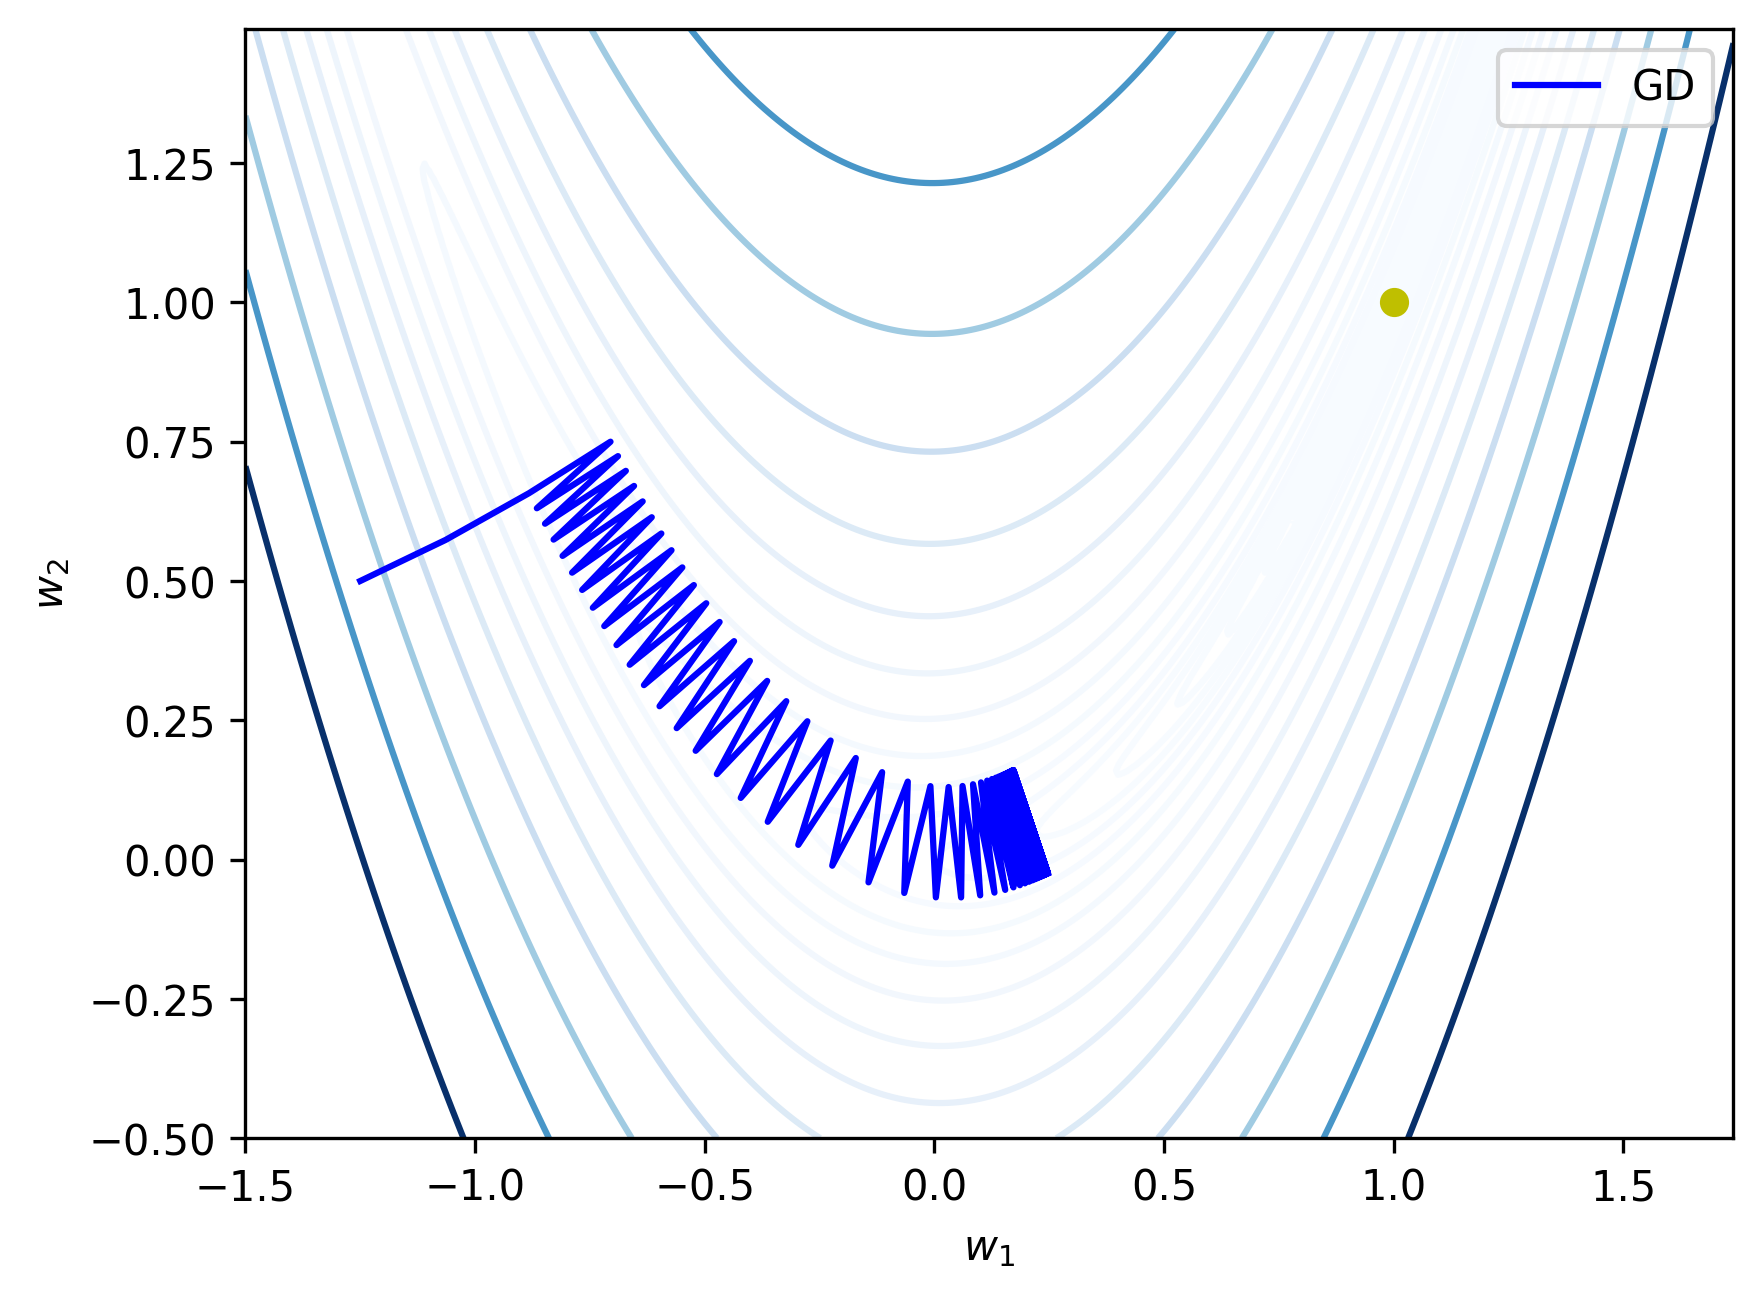
\includegraphics[width=0.6\linewidth]{chapters/neural/images/gd_oscillating.png}
	\caption{Работа градиентного спуска при минимизации функции Розенброка. Метод всегда шагает на фиксированное расстояние чтобы было видно осцилляции.}
	\label{img:gd_osc}
\end{figure}

На решение этих проблем и направлены различные эвристики и обобщения, которые мы рассмотрим далее.

\begin{problem}[Медленная сходимость градиентного спуска.]
Пусть минимизируемая функция имеет следующий вид: $\mathcal{L}(w, x) = (w - w^*)^T M (w - w^*)$, где $M \in \mathbb{R}^{m \times m}$~--- положительно определенная матрица с собственными числами $\lambda_1 = 1$, $\lambda_m = 10^{-4}$. Вычислите величину градиентного шага  $h$, при которой градиентный спуск с постоянным шагом будет гарантированно сходиться. Сколько при такой величине шага потребуется итераций для достижения требуемой точности $\varepsilon$, если точка старта $x_0 = v_m$, где $v_m$~--- собственный вектор матрицы $M$, соответствующий собственному числу $\lambda_m$ и имеющий единичную норму?
\end{problem}

\begin{remark}
Сценарий из этой задачи особенно части встречается, если не отнормировать данные перед обучением модели. 
\end{remark}

\subsection{Метод накопления инерции}

Чтобы избежать осцилляций и сделать стохастический градиентный спуск более плавным, можно добавить градиенту <<инерцию>>, и усреднять его значение по последним нескольким шагам. Тогда получится метод \textbf{Momentum}, или метод тяжелого шарика, изобретенный Б. Т. Поляком в 1964 г. Его метод обновления весов может быть записан так:
\begin{align*}
v &:= \gamma v + (1 - \gamma) \mathcal{L}'(w, x_i) \\
w &:= w - h v\,,
\end{align*}
где параметр $h$ отвечает за величину шага, а $\gamma$~--- за то, насколько сильно предыдущие итерации будет влиять на текущую.

Развил эту идею Ю. Е. Нестеров, в 1983 г. предложив метод \textbf{NAG} (Nesterov's accelerated gradient). В нём градиент не только усредняется по нескольким итерациям, но и <<подглядывает>> вперед в направлении своего движения, и обновляет веса с учетом полученной информации:
\begin{align*}
v &:= \gamma v + (1 - \gamma) \mathcal{L}'(w - h \gamma v, x_i) \\
w &:= w - h v\,,
\end{align*}

Эти методы хорошо показали себя при обучении больших нейросетевых моделей. По сравнению с стохастическим градиентным спуском они обладают большей устойчивостью к выбросам, меньше осциллируют.

\begin{figure}[h]
	\centering
	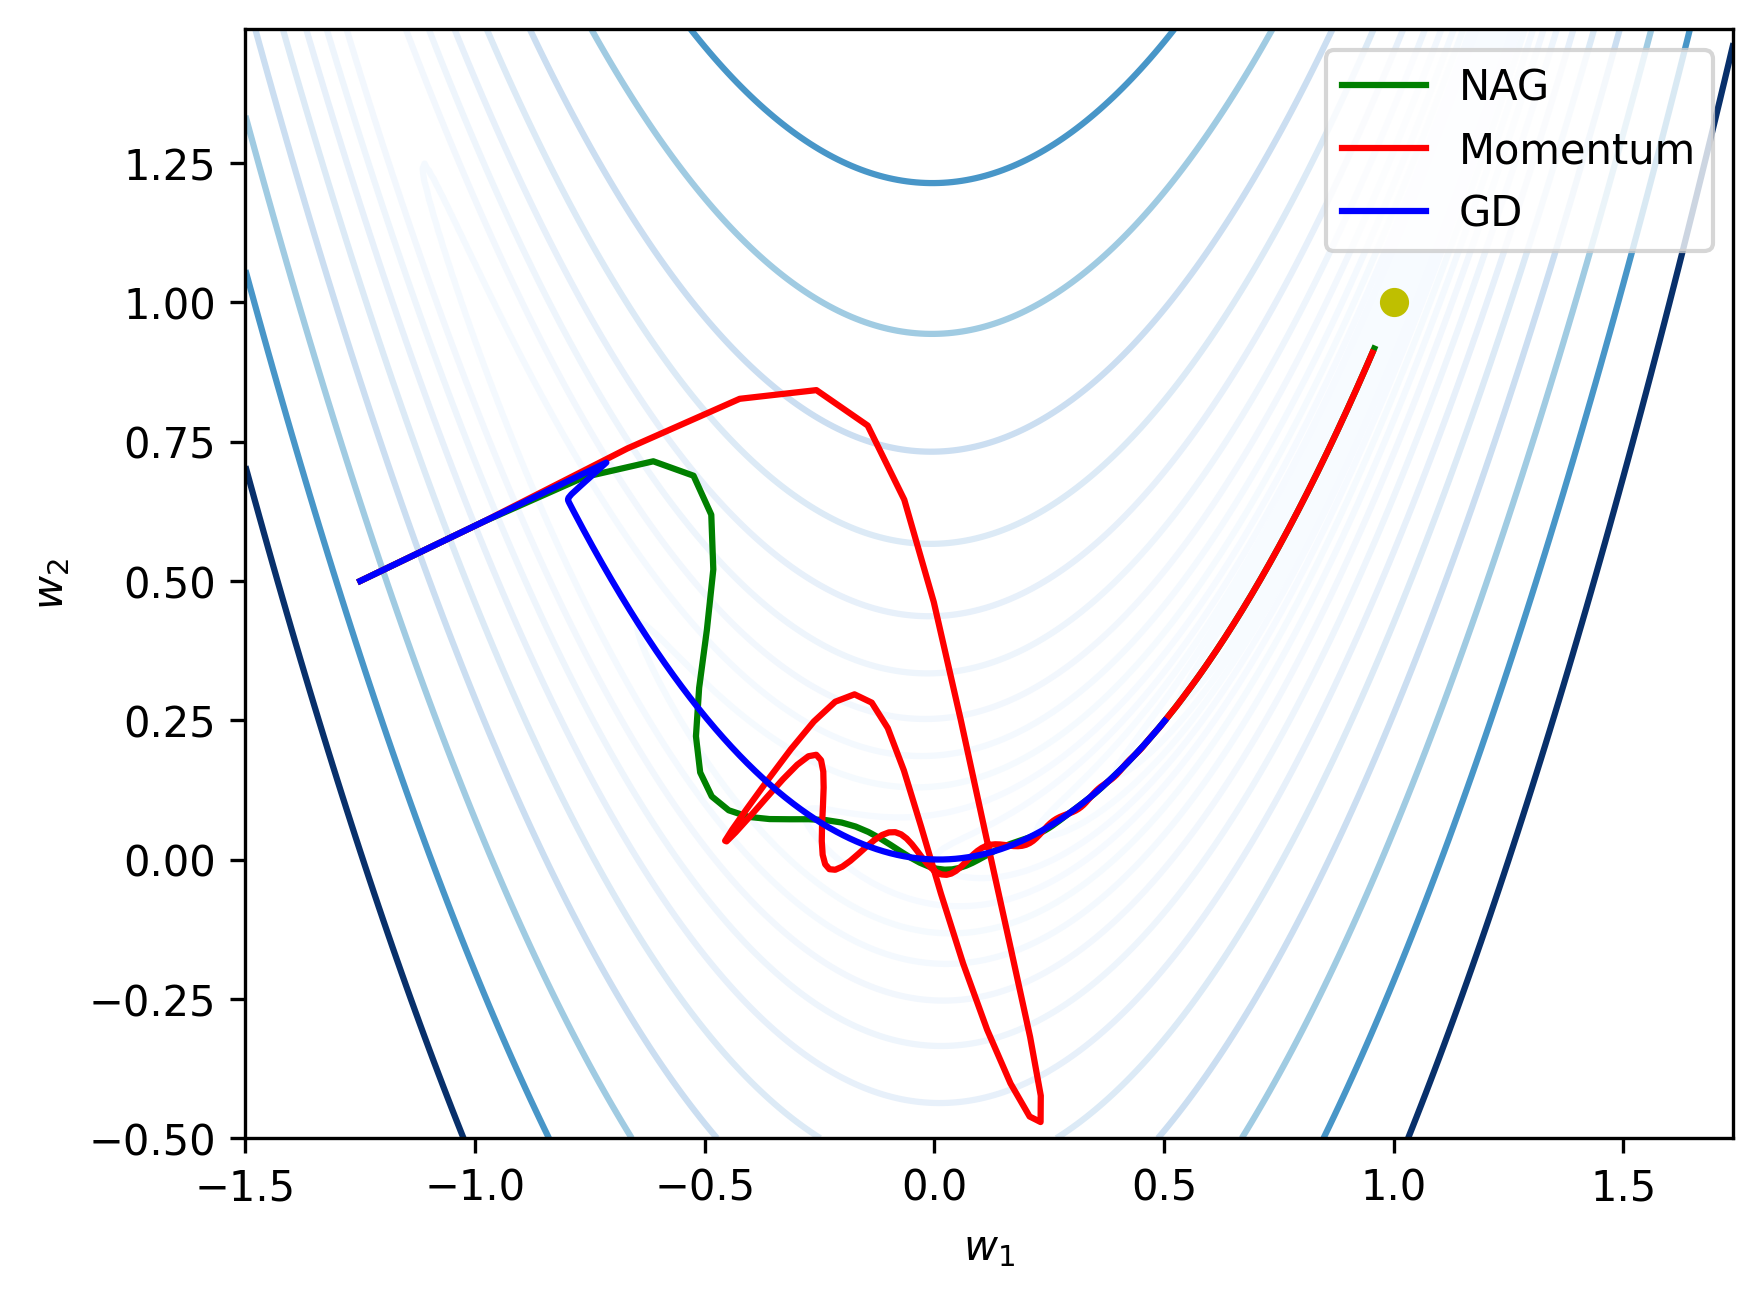
\includegraphics[width=0.6\linewidth]{chapters/neural/images/nag_momentum_gd.png}
	\caption{Пример работы методов Momentum, NAG и градиентного спуска при оптимизации функции Розенброка. Все методы делают $10^4$ итераций.}
	\label{img:gd_osc}
\end{figure}

\subsection{Варианты инициализации весов}

Чтобы улучшить сходимость метода можно правильно инициализировать веса модели. Возможно очень много различных вариантов, например:
\begin{enumerate}
    \item $w_j := 0$ для всех $j=1,\dots,n$;
    \item Небольшие случайные значения, $w_j := \text{random}\left(-\frac{1}{2n}, \frac{1}{2n}\right)$;
    \item Обучение по небольшой стартовой предвыборке объектов;
    \item Мультистарт: многократные запуски из различных случайных начальных приближений и выбор лучшего из них;
    \item В случае линейной регрессии, $w_j := \frac{\langle y, f_j \rangle}{\langle f_j, f_j \rangle}$, где $f_j = (f_j(x_i))_{i=1}^l$.
\end{enumerate}

\begin{problem}[Смысл 5 способа инициализации весов.]
Покажите что в модели линейной регрессии с квадратичной функцией потерь и некореллированными признаками ($\langle f_j, f_k \rangle = 0,\ j \neq k$), веса, полученные с помощью оценки 5 на самом деле являются точным решением задачи оптимизации.
\end{problem}

\subsection{Варианты порядка предъявления объектов}

Метод стохастического градиента чувствителен к тем способу предоставления новых оъектов на каждом шаге. Для улучшения сходимости можно применить одну из следующих эвристик:

\begin{enumerate}
    \item Перетасовка объектов (shuffling). Можно перемешивать объекты, брать попеременно объекты из разнвх классов. Это помогает избежать переобучения если объекты, например, хранятся в хронологическом порядке.
    \item Чаще брать объекты на которых функция потерь принимает большие значения. Это помогает нейросети выучить сложные примеры, даже если в выборке их немного.
\end{enumerate}

В задачах многоклассовой классификации также можно применять следующие техники:
\begin{enumerate}
    \item В задачах классификации чаще брать объекты на которых меньше уверенность (margin).
    \item Вообще не брать <<хорошие>> объекты на которых margin больше константы $\mu_+$. Это может ускорить сходимость.
    \item Вообще не брать объекты <<выбросы>> на которых margin меньше константы $\mu_-$. Это может улучшить качество классификации. 
\end{enumerate}
В этих случаях константы $\mu_+$ и $\mu_-$ придется подбирать.

\subsection{Варианты выбора градиентного шага}

Вообще говоря, сходимость метода стохастического градиента с фиксированным шагом это чудо~--- даже для выпуклых функций метод будет осциллировать в окрестности минимума. Чтобы бороться с проблемой осцилляций можно варьировать величину градиентного шага.

\begin{enumerate}
    \item Можно уменьшать величину шага с каждой итерацией. В таком случае для выпуклых функций сходимость гарантируется если:
    \[
    h_t \rightarrow 0,\, \sum_{t = 1}^{\infty} h_t = \infty,\, \sum_{t=1}^{\infty} h_t^2 < \infty
    \]
    В частности можно положить $h_t = 1 / t$.
    \item Можно на каждом шаге выбирать величину шага, минимизирующую функцию одной переменной:
    \[
    \mathcal{L}(w - h \nabla \mathcal{L}(w, x_i), x_i) \rightarrow \min_h\,.
    \]
    Это называется \textbf{метод скорейшего градиентного спуска}.
    \item Можно делать случайные <<пробные>> шаги, которые помогут <<выбить>> функцию из неглубокого локального минимума.
\end{enumerate}

\begin{figure}[h]
	\centering
	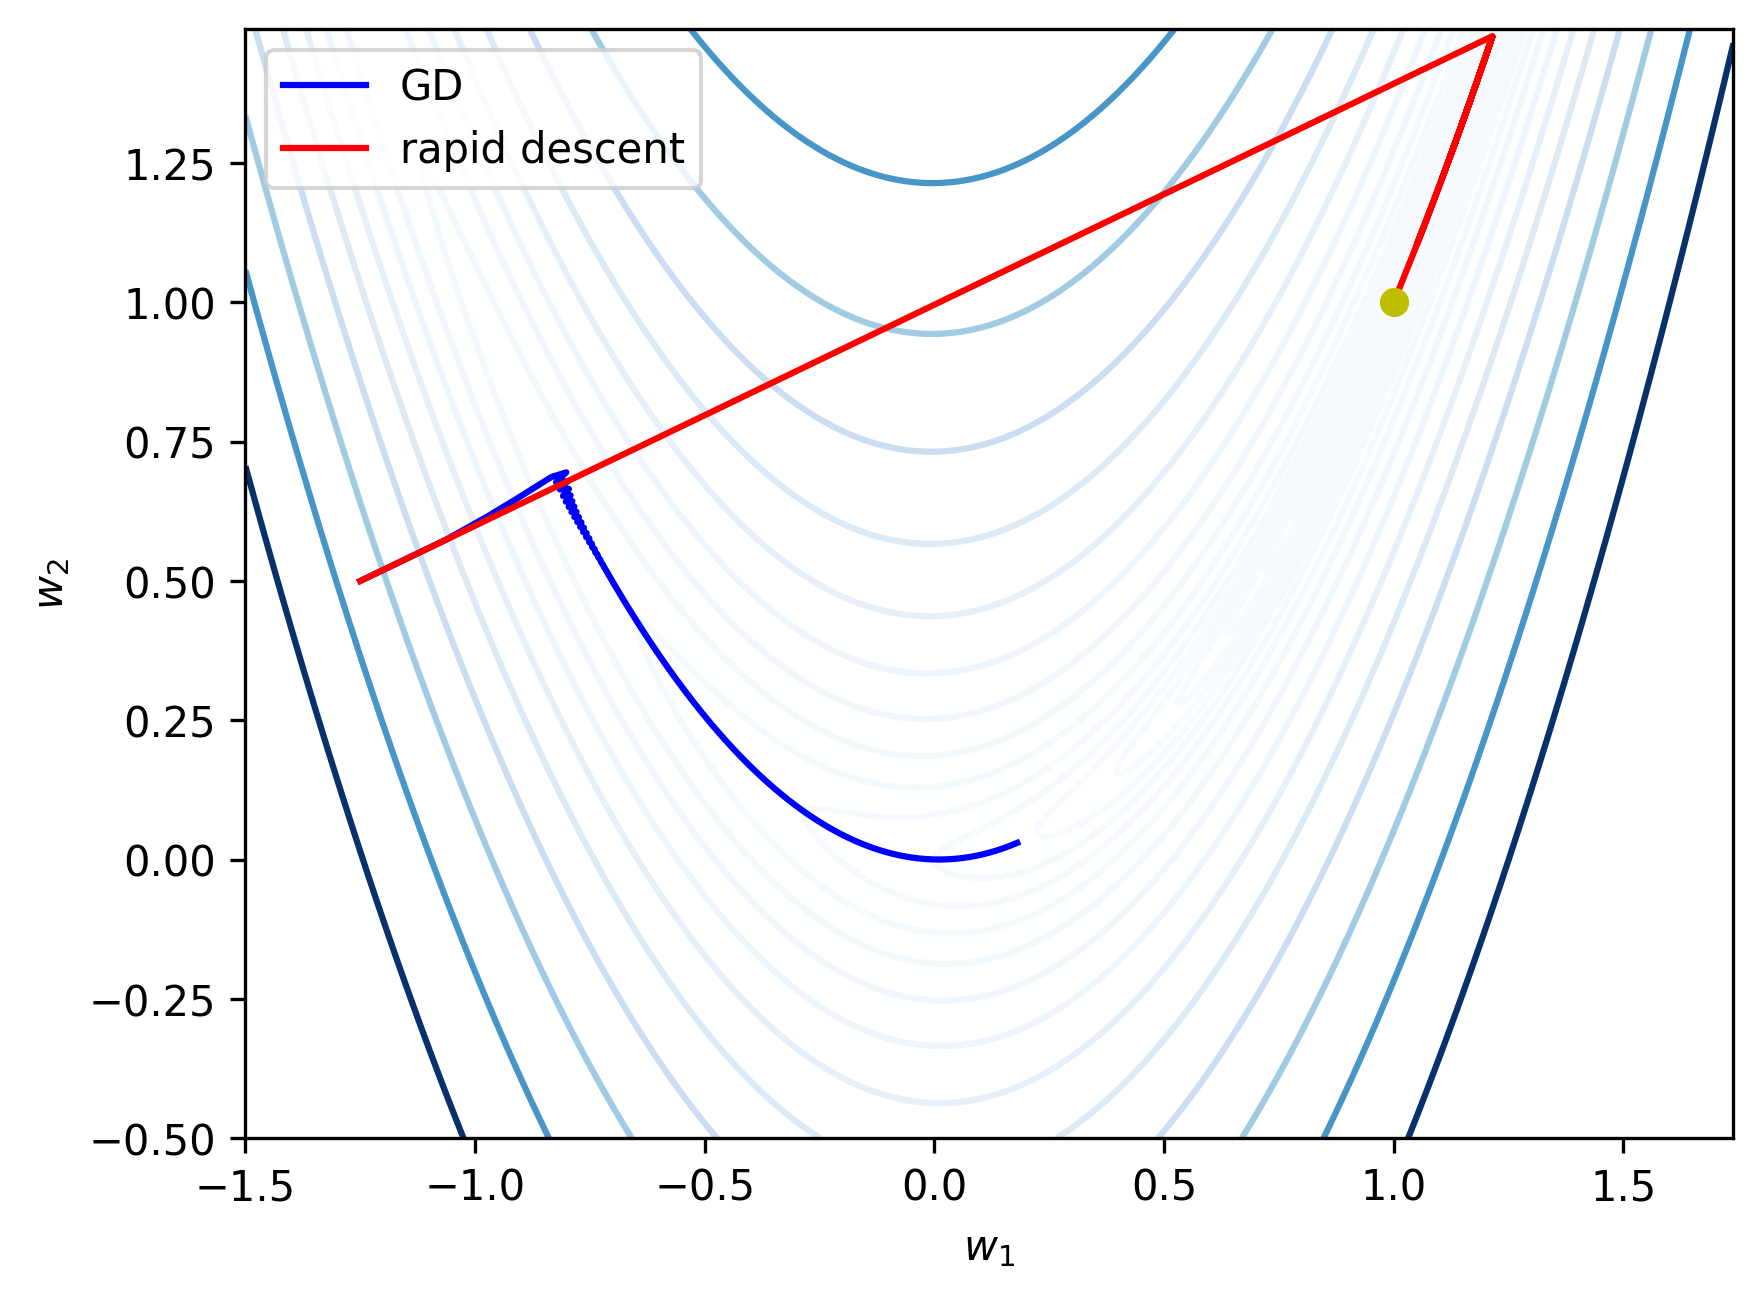
\includegraphics[width=0.6\linewidth]{chapters/neural/images/gd_rd_example.png}
	\caption{Работа градиентного спуска и скорейшего градиентного спуска при минимизации функции Розенброка. Оба метода делают $10^4$ итераций.}
	\label{img:gd_osc}
\end{figure}

\begin{remark}
Существуют и более продвинутые алгоритмы, модифицирующие величину градиентного шага, такие как Adagrad, RMSProp, Adadelta, а также методы, сочетающие идеи подстройки градиентного шага и накопления момента, такие как Adam, Adamax, Nadam. Часть их них будет рассмотрена в последующих параграфах.
\end{remark}

\subsection{Методы второго порядка}

Методы второго порядка используют не только градиент функции, но и ее гессиан. Это может дать очень хорошие результаты, например метод не будет застревать в седловых точках. Методы второго порядка предоставляют более быструю сходимость и точность ценой вычислительной эффективности, и в больших задачах они обычно не применяются.

Самый первый из методов второго порядка~--- многомерный метод Ньютона. Его итерацию можно записать как:
\[
w := w - \left(\nabla^2\mathcal{L}(w, x_i)\right)^{-1}\nabla \mathcal{L}(w, x_i)\,.
\]
Исходно метод Ньютона был предназначен для нахождения нуля функции, и выражение выше представляет собой просто-напросто метод для поиска нулей Гессиана. Однако в такой базовой формулировке метод очень часто расходится, и применятются его различные модификации, такие как метод Ньютона-Рафсона:
\[
w := w - h\left(\nabla^2\mathcal{L}(w, x_i)\right)^{-1}\nabla \mathcal{L}(w, x_i)\,.
\]
где $h$ может быть как постоянной, так и выбираться из соображений минимизации одномерной функции, как в методе скорейшего градиентного спуска.

Есть и огромное количество других обобщений, например метод Левенберга-Маквардта, который представляет собой суперпозицию методов Ньютона-Рафсона и обычного градиентного спуска.

\begin{problem}[Сравнение методов первого и второго порядков]
    Докажите, что если минимизируемая функция квадратична, $\mathcal{L}(w, x) = (w - w^*)^T M (w - w^*)$, где $M$~--- положительно определенная матрица, метод Ньютона сойдется к минимуму за одну итерацию. Сравните вычислительную алгоритма сложность с той, которую вы получили в первой задаче для $\varepsilon = 10^{-8}$
\end{problem}

\section{Функции активации ReLU и PReLU. Проблема «паралича» сети.}
\subsection{Про функции активации}

Функция активации в контексте нейронных сетей определяет выходной сигнал нейрона на основе входного сигнала или набора входных сигналов. Она играет важную роль в определении нелинейности модели и позволяет нейронной сети обучаться сложным зависимостям между входными данными и выходами, а также влияеть на эффективность обучения модели.(грубо говоря определяет будет ли нейрон активирован - даст не нулевой выход) \\
В искусственных нейронных сетях используются различные типы функций активации, такие как тождественная функция, ступенчатые функции, сигмоидные функции и многие другие. \\
\textbf{Важным требованием} к функции активации является ее нелинейность, чтобы нейронная сеть могла эффективно справляться с нетривиальными задачами.\\ Примером широко используемой функции активации является ReLU.

\subsection{ReLU (Rectified Linear Unit), проблема «паралича» сети}

\textbf{\textit{Определение:}} 
Функция активации ReLU определяется как:
$f(x) = max(0, x)$, где x — входное значение.\\
Не смотря на очевидную простоту функции активации ReLU, у неё есть одна существенная проблема: она может вызывать так называемый \textbf{«паралич» сети}.\\
Если градиент весов становится слишком большим, то некоторые нейроны могут получить очень большие отрицательные веса, что приведёт к тому, что их выходные значения всегда будут равны нулю независимо от входного сигнала. Эти нейроны становятся неактивными («замороженными») и больше не участвуют в процессе обучения. Если это происходит слишком часто, то это может привести к ухудшению результата.\\
Для решения этой проблемы была предложена модификация ReLU.
\subsection{PReLU (Parametric Rectified Linear Unit)}

\textbf{\textit{Определение:}}
Функция PReLU является обобщением ReLU и определяется как:
$$ f(x) = \begin{cases}
x & \text{if } x > 0 \\
\alpha x & \text{if } x \leq 0
\end{cases} $$
В отличие от обычной ReLU, где все отрицательные значения обнуляются, PReLU вводит дополнительный параметр $\alpha$, который управляет наклоном линии для отрицательных значений. Этот параметр $\alpha$ может быть обучен вместе с другими параметрами сети, что позволяет избежать полного отключения нейронов. То есть даже отрицательный входной сигнал будет вносить вклад в обучение модели, что уменьшает проблему паралича сети и улучшает получаемый результат.

\subsection{Задачи}
\textbf{Задача 1}

Представьте, что вы получили графики функций активации ReLU и PReLU (с заданным параметром $\alpha$) для различных входных значений.\\
Опишите, как выглядит график функции активации ReLU и как он отличается от графика PReLU. Какова роль параметра $\alpha$ в PReLU?\\
\textbf{Решение}

График функции ReLU выглядит как угол, который начинается от нуля и идет вверх с углом 45 градусов для положительных значений.\\
График функции PReLU (Parametric ReLU) также имеет две части, но для отрицательных значений он не обрезается до нуля. Вместо этого, он наклонен под углом, определяемым параметром $\alpha$. \\
Роль параметра $\alpha$ в PReLU:\\
Параметр $\alpha$ определяет наклон линии для отрицательных значений. Если $\alpha$ велико, то выход будет относительно большим даже для небольших отрицательных входов, что позволяет нейрону сохранять некоторую активность. Если $\alpha$ близко к нулю, то функция будет почти горизонтальной для отрицательных значений, что делает нейрон менее активным в этом диапазоне.\\
\textbf{Задача 2.1}

Рассмотрим простой случай использования функции активации ReLU в одном слое нейронной сети. Пусть входной сигнал равен $-4$, а вес этого нейрона равен $10$. Каково будет значение на выходе этого нейрона после применения функции активации ReLU?\\
\textbf{Решение:}

Выходной сигнал до применения функции активации будет равен произведению входа и веса: $-4 \cdot 10 = -40$. После применения функции активации ReLU получаем: $f(-40) = \max(0, -40) = 0$. Таким образом, этот нейрон станет неактивным ("замороженным"), поскольку его выходной сигнал всегда будет нулевым независимо от изменения входного сигнала.\\
\textbf{Задача 2.2}

Пусть теперь используется функция активации PReLU с параметром $\alpha = 0.01$. Рассчитайте значение на выходе того же нейрона, что и в предыдущей задаче, но уже с использованием PReLU.\\
\textbf{Решение:}

После умножения входа и веса получаем тот же результат: $-4 \cdot 10 = -40$. Теперь применяем функцию активации PReLU:

$$ f(-40) = \begin{cases}
-40 & \text{if } (-40) > 0 \\
0.01 \cdot (-40) & \text{if } (-40) \leq 0
\end{cases} $$

Так как $-40 \leq 0$, мы используем вторую часть определения функции: $f(-40) = 0.01 \cdot (-40) = -0.4$. В этом случае нейрон не становится полностью замороженным, так как его выходной сигнал остается отличным от нуля даже при отрицательном входе.\\
\textbf{Задача 3}

Входной сигнал $x$ распределён равномерно на интервале [-10, 10], а вес $w$ нейрона равен 2, параметр $\alpha = 0.1$.\\
Какова вероятность, что нейрон заморозится при использовании каждой из функций ReLU и PReLU?\\
\textbf{Решение:}\\
Для ReLU:\\
Нейрон «замораживается», если выходной сигнал после применения функции активации всегда равен нулю. То есть, если $wx <= 0$.\\
Поскольку $w = 2$, условие $wx <= 0$ эквивалентно $x <= 0$.\\
Вероятность того, что $x$ окажется меньше или равно нулю, равна вероятности того, что $x$ попадет в интервал -10, 0. \textit{Это составляет половину всего диапазона распределения, поэтому вероятность равна 0.5.}\\
При использовании PReLU нейрон никогда не «замерзнет», потому что даже при отрицательных значениях $x$ выходной сигнал будет отличен от нуля благодаря параметру $\alpha$.
\textit{Таким образом, вероятность того, что нейрон «заморозится», равна 0.}

\section{Drop Out}
\subsection{Теоретические сведения}

\textbf{Drop Out} (метод отключения случайных нейронов) - это метод, который представляет собой эффективный подход к борьбе с переобучением в полносвязных нейронных сетях. 

Переобучение может происходить, когда нейроны в сети начинают "запоминать" шум и особенности обучающего набора, вместо того чтобы извлекать общие закономерности. Во время обучения нейронной сети нейроны взаимодействуют друг с другом, и иногда происходит так, что один нейрон начинает исправлять ошибки другого. Это может привести к ситуации, когда в одном слое нейронов образуются большие веса с разными знаками, что делает модель менее стабильной и затрудняет ее обобщение. В таких случаях, даже если модель демонстрирует высокую точность на обучающих данных, она может оказаться неэффективной на тестовых данных.

Идея Drop Out заключается в том, что при обучении случайные нейроны отключаются (то есть возвращают всегда нулевое значение) и не участвуют в данном шаге обучения. В таком случае большие значения весов разных знаков не всегда участвуют в обучении одновременно, и модель стабилизируется.

Обучение с Dropout можно интерпретировать как обучение одновременно $2^N$ моделей (где $N$ ~--- количество нейронов) с разными архитектурами связей. При обучении выбирается модель, наиболее устойчивая к потере доли нейронов; разные части модели решают одну и ту же задачу вместо того, что бы компенсировать ошибки друг друга.

Недостатком Drop Out является более долгое обучение модели в связи со случайностью процесса обучения.

\subsection{Реализация}
При обучении выбирается параметр $p$ ~--- вероятность отключения. Модель обучается с отключением случайных нейронов. Можно отключать в каждом слое долю $p$ нейронов, вместо независимого отключения, чтобы избежать полного отключения одного слоя.

$$x_i^l = \xi_i^l \sum_{j=1}^{K_{l-1}} w_{ij}^l x_j^{l-1} $$

$l$ ~--- номер текущего слоя, $i$ ~--- номер нейрона в этом слое, $K_l$ ~--- кол-во нейронов в слое $l$, $\xi \sim Be(1-p)$ ~--- случайная величина, отвечающая за отключение.

$\left[\xi_i^l\right] = 1-p$, поэтому на этапе применения вводится нормировка:
$$x_i^l = (1-p) \sum_{j=1}^{K_{l-1}} w_{ij}^l x_j^{l-1} $$

Чаще используется \textbf{Inverted Drop Out} для простоты применения:

$$x_i^l = \frac{\xi_i^l}{1-p} \sum_{j=1}^{K_{l-1}} w_{ij}^l x_j^{l-1} $$
~--- при обучении;

$$x_i^l = \sum_{j=1}^{K_{l-1}} w_{ij}^l x_j^{l-1} $$
~--- при применении.

\subsection{Задачи}
\begin{description}
\item[\textbf{Задача 1}] 
    Какие по порядку величины должны быть ограничения на значения $p$, чтобы избежать отключения одного слоя целиком?
\item[\textbf{Решение:}] если в сети $L$ слоёв размерности $K$, то $p \sim (\frac{c}{L})^{1/K}. $
    Тогда вероятность отключения одного слоя $p^K = \frac{c}{L}; $ вероятность функционирования всех слоёв: $\sim (1-p^K)^L = (1-\frac{c}{L})^L \sim e^{-c}$.
    
    Если взять $c\sim 0.01$ , получим вероятность работы сети $\sim 99\%$.
    
    Если $L=4, K=10,$ то $p \sim 54\%$.

\

\item[\textbf{Задача 2}] 
    Сколько шагов обучения нужно провести, чтобы не осталось нейронов, которые были бы выкинуты на каждом шаге (то есть совсем не обучались)?

\item[\textbf{Решение:}] если в сети $N$ нейронов, то вероятность одному нейрону совсем не обучиться в течение $T$ итераций равна $p^T$. Тогда среднее число необученных нейронов равно $Np^T$. Из условия $Np^T<1$ получаем $T>-\log_{p}N = \frac{\ln N}{\ln \frac{1}{p}}$.



%%%%%%%%%%%%%%%%%%%%%%%%%%%%%%%%%%%%%%%%%%%%%%%%%%%%%%%%%%%%%%%%%%%%%%%%%%%%%%%%%%%%%%%%%%%%%%%%%%%%%%%%%%%%%%%%%%%%%%%%%%%%%%%%%%%%%%%%%%%%%%%%%%%%%%%%%%%%%%%%%%%%%%%%%%%%%%%%%%%%%%%%%%%%%%%%%%%%%%%%%%%%%%%%%%%%%%%%%%%%%%%%%%%
\section{Персептрон и модель Изинга}

Персептрон является одной из базовых моделей машинного обучения и может быть интерпретирован как аналог физических систем, в частности, неоднородной модели Изинга. 
Эти аналогии вдохновили развитие ограниченных машин Больцмана (RBM), которые минимизируют энергетическую функцию, что позволяет создавать более устойчивые модели машинного обучения.  

Пусть имеется решётка, на каждом узле которой $i = 1, \dots, N$ расположена дискретная переменная, принимающая одно из двух состояний: $s_i = +1$ или $s_i = -1$. Эти состояния удобно называть \textit{спинами} (или нейронами в контексте персептрона), где $s_i = +1$ соответствует спину вверх, а $s_i = -1$ — спину вниз. 
Взаимодействие отдельного нейрона с остальными нейронами можно выразить через энергетическую функцию:
\[
E[S] = - \sum_i B_i S_i -\sum_{\langle i j \rangle} J_{ij} S_i S_j,
\]
где:
\begin{itemize}
    \item $S_i \in \{-1, 1\}$ — состояние спина;
    \item $J_{ij}$ — коэффициенты взаимодействия;
    \item $B_i$ — внешнее поле.
\end{itemize}
Если в модели присутствует только первый член, то нейроны не взаимодействуют друг с другом, и модель решается тривиально. Второй член отвечает за взаимодействие между соседними нейронами. Обозначение $\langle i j \rangle$ означает, что сумма берётся по всем парам ближайших соседей в решётке.

В отличие от классической модели Изинга, где взаимодействия между спинами задаются фиксированными параметрами $B$ и $J$, в данном подходе (аналогия с полевой теорией Гинзбурга–Ландау) эти параметры являются обучаемыми. Их значения уточняются в процессе обучения нейронной сети.

В вероятностной интерпретации модель Изинга описывается распределением Гиббса:
\[
P(S) = \frac{1}{Z} e^{-\beta E},
\]
где $Z$ — статистическая сумма:
\[
Z = \sum_{\{S_i\}} e^{-\beta E},
\]
а $\beta$ — это обратная температура 
 + нормировка, $\beta = \frac{1}{k_B T}$. При 
$T\rightarrow0$: сеть ведет себя как дискретная оптимизация (модель Изинга).
При $T \rightarrow \infty$: сеть становится шумной, склонной к случайным состояниям.(См. задача.)

С другой стороны, \textbf{Формула активации для бинарного персептрона:}
\[
y = \mathrm{sign}\left(\sum_{i=1}^n w_i x_i + w_0\right),
\]
где:
\begin{itemize}
    \item $x_i$ — входной сигнал;
    \item $w_i$ — вес связи;
    \item $w_0$ — смещение (bias);
    \item $\mathrm{sign}$ — функция активации, возвращающая $+1$ или $-1$.
\end{itemize}

Здесь веса $w_i$ и сигналы $x_i$ можно рассматривать как аналоги $J_{ij}$ и $S_i$, а функция активации $\mathrm{sign}$ моделирует взаимодействие спинов в системе.

Энергетическая функция $E$ в модели Изинга может быть интерпретирована как функция потерь в персептроне:
\[
E = - \mathbf{w}^\top \mathbf{x},
\]
где $\mathbf{w}$ — вектор весов, а $\mathbf{x}$ — входной вектор.

Минимизация энергии в модели Изинга аналогична обучению персептрона, где цель состоит в подборе весов, минимизирующих ошибку классификации.

\subsection{Функции активации и их физический смысл}

Рассмотрим однослойную нейронную сеть размерности $N - 1$ во внутреннем слое с нейронами $s_i$ и одним выходным нейроном $s_1$. Пусть на вход подаётся вектор размерности $M$. В качестве функции активации на выходном нейроне часто используется гиперболический тангенс:
\[
\mathrm{tanh}(B) = \frac{e^{B} - e^{-B}}{e^{B} + e^{-B}}, \quad -B = w_0 + \sum_i w_i s_i.
\]

Как будет показано далее, его выбор связан не только с асимптотическим поведением и хорошими гладкими свойствами. 

Рассмотрим статистическую сумму невзаимодействующих нейронов, умноженную на единицу:
\[
Z[J] = \left.\sum_{\{s_i\}} e^{-B s_i} e^{J s_i} \right|_{J=0}, \quad s_i \in \{\pm 1\}.
\]
Средняя энергия статистических систем определяется как, оно же мат ожидание нейрона $s$ опрделеяется:
\[
\langle s \rangle = \frac{1}{Z} \frac{\partial}{\partial J} Z = \frac{1}{Z} \sum_{\{s_i\}} e^{-B s_i + J s_i} s_i \bigg|_{J=0} = \tanh(-B).
\]
Таким образом, гиперболический тангенс представляет собой среднюю энергию спиновой системы в модели Изинга и моделирует взаимодействие спинов с одной стороны, и с другой, представляет из себя функцию потерь $\mathcal{L}$  персептрона.

\subsubsection*{Распределение нейронов в сети}

Если состояния нейронов скрытого слоя $i \in [2, N]$ известны, они выражаются через компоненты входного вектора и веса модели:
\[
P(s_i) = \frac{1}{Z_i} \exp\left[ w_{0i} s_i + \sum_{j=1}^M w_{ij} s_i x_j \right].
\]
Тогда вероятностное распределение выходного нейрона $i = 1$ задаётся как:
\[
P(s_1 | s_2, s_3, \dots, s_N) = \frac{1}{Z_1} \exp\left[ s_1 \left( w_{01} + \sum_{i=2}^N w_{i1} s_i \right) \right].
\]

Полное вероятностное распределение выходного нейрона будет иметь вид:
\[
P(s_1) = P(s_1 | s_2, \dots, s_N) \prod_{i=2}^N P(s_i) = \frac{1}{\prod_{i=1}^N Z_i} \exp\left[ \sum_{i=1}^N w_{0i} s_i + \sum_{i,j=2}^{N,M} w_{ij} s_i x_j + s_1 \sum_{j=1}^M w_{ij} s_j \right].
\]

Запишем это в терминах модели Изинга:
\[
P(s_1) = \frac{1}{Z} \exp\left[-\sum_i B_i s_i - \sum_{i,j} J_{ij} s_i s_j \right],
\]
где $B_i$ — магнитное поле, а $J_{ij}$ — взаимодействие нейронов, которые выражаются через веса. В процессе обучения модели (backpropagation) задача состоит в определении значений $B_i$ и $J_{ij}$.
Нахождение распределения вероятностей в сети соответствует решению задачи минимизации энергии модели Изинга.

\subsection{Задачи}
\textbf{Задача 1:} Покажите, что вероятностная интерпретация модели Изинга связана с логистической регрессией.

\textbf{Решение:}
Логистическая регрессия основана на функции активации:
\[
\sigma(x) = P(y=1 | x) = \frac{1}{1 + e^{-E}}, \quad E = \mathbf{w}^\top \mathbf{x} + w_0.
\]

Для модели Изинга распределение вероятностей:
\[
P(S = 1) = \frac{e^{-E}}{e^{E} + e^{-E}} = \frac{1}{1+ e^{2E}} =  \sigma(-2E),\quad P(S = -1) = \sigma(2E).
\]
что аналогично модели логистической регрессии с сигмоидальной функцией вероятности.
\textbf{Задачи 2 - 3:}  
Модель весов \( W \) персептрона имеет специальную структуру:
\[
W = \text{Diag}(d_1, d_2, \dots, d_N) + \mathbf{x} \mathbf{x}^\top,
\]
где \( \text{Diag}(d_1, d_2, \dots, d_N) \) — диагональная матрица, а \( \mathbf{x} \mathbf{x}^\top \) — внешнее произведение входного вектора \( \mathbf{x} \). Энергия системы(она же функция потерь) определяется как:
\[
E = -\mathbf{s}^\top W \mathbf{s},
\]
где \( \mathbf{s} \in \{-1, +1\}^N \).

\begin{enumerate}
    \item Найти состояние \( \mathbf{s} \), минимизирующее энергию \( E \).
    \item Найдите общее условие на W, при котором система имеет как минимум два устойчивых состояния $s_1$ и $s_2$. 
\end{enumerate}

\textbf{Решение:}

1. \textbf{Минимум функции энергии:}

Энергия \( E \) принимает вид:
\[
E = -\mathbf{s}^\top \text{Diag}(d_1, \dots, d_N) \mathbf{s} - \mathbf{s}^\top (\mathbf{x} \mathbf{x}^\top) \mathbf{s}.
\]

Первый член:
\[
-\mathbf{s}^\top \text{Diag}(d_1, \dots, d_N) \mathbf{s} = -\sum_{i=1}^N d_i s_i^2.
\]
Так как \( s_i^2 = 1 \) для \( s_i \in \{-1, +1\} \), получаем:
\[
-\mathbf{s}^\top \text{Diag}(d_1, \dots, d_N) \mathbf{s} = -\sum_{i=1}^N d_i.
\]

Второй член:
\[
-\mathbf{s}^\top (\mathbf{x} \mathbf{x}^\top) \mathbf{s} = -(\mathbf{x}^\top \mathbf{s})^2.
\]

Таким образом, энергия принимает вид:
\[
E = -\sum_{i=1}^N d_i - (\mathbf{x}^\top \mathbf{s})^2.
\]

Энергия минимизируется, когда \( (\mathbf{x}^\top \mathbf{s})^2 \) максимально. Это достигается, если компоненты вектора \( \mathbf{s} \) сонаправлены с компонентами \( \mathbf{x} \). То есть:
\[
s_i = \text{sign}(x_i), \quad i = 1, \dots, N.
\]

2. \textbf{Устойчивые состояния:}

Поскольку \( W \) симметрична, энергия может быть минимизирована, если состояния \( \mathbf{s} \) совпадают с собственными векторами матрицы \( W \), соответствующими наименьшим собственным значениям.

\begin{itemize}
    \item Один собственный вектор — это \( \mathbf{x} \) с собственным значением \( \|\mathbf{x}\|^2  + \overline{d}\) (d - взвешенного диагонального элемента по направлению x),
    \item Остальные \( N-1 \) собственных значений равны диагональным элементам \( d_i \).
\end{itemize}

Если \( \|\mathbf{x}\|^2 \gg d_i \), то устойчивое состояние \( \mathbf{s} \) сонаправлено с \( \mathbf{x} \). Если \( d_i \) доминируют, состояние определяется диагональными элементами.

Кроме того, симметрия матрицы \( W \) означает, что если \( \mathbf{s}^* \) минимизирует энергию, то \( -\mathbf{s}^* \) тоже является решением, так как:
\[
E(-\mathbf{s}^*) = E(\mathbf{s}^*).
\]

\textbf{Задача*} 

1. Рассмотрим однослойную нейронную сеть с \( N \) нейронами в скрытом слое и одним выходным нейроном. На вход поступает вектор \( \mathbf{x} \in \mathbb{R}^M \), веса имеют случайные значения \( w_i \sim \mathcal{N}(0, \sigma^2) \), а функция активации на выходном нейроне задается как:
   \[
   s_\text{out} = f\left( \sum_{i=1}^N w_i \cdot s_i + w_0 \right),
   \]
   где \( f(x) = \mathrm{tanh}(\beta x), \beta = 1/T \).

Что произойдет с выходом \( s_\text{out} \) при \( T \to \infty \) и \( T \to 0 \), если считать, что активация тангенса моделирует энергетическое состояние спиновой системы? 

2. Рассмотрим предельный случай, когда число нейронов \( N \to \infty \), а веса \( w_i \) независимы и одинаково распределены. Покажите, что результатирующее распределение выхода \( s_\text{out} \) будет стремиться к гауссовскому. В каком случае это приближение применимо?

\textbf{Решение:}

\subsubsection*{1. Поведение нейронной сети при \( T \to \infty \) и \( T \to 0 \)}

\textbf{При \( T \to \infty \):}
Гиперболический тангенс \( \mathrm{tanh}(\beta x) \) стремится к линейной функции:
\[
\mathrm{tanh}(\beta x) \approx \beta x \quad \text{при } \beta \to 0 \, (T \to \infty).
\]
Нейронная сеть теряет нелинейность, и выход становится линейной комбинацией входов:
\[
s_\text{out} \approx \beta \left( \sum_{i=1}^N w_i s_i + w_0 \right).
\]
Поведение сети приближается к \textbf{линейной модели}.

\textbf{При \( T \to 0 \):}

Гиперболический тангенс становится почти пороговой функцией:
\[
\mathrm{tanh}(\beta x) \to 
\begin{cases} 
-1, & x < 0, \\ 
1, & x > 0.
\end{cases}
\]
Нейронная сеть превращается в \textbf{дискретную систему}, где выходные значения строго определяются знаком линейной комбинации входов:
\[
s_\text{out} = \text{sign} \left( \sum_{i=1}^N w_i s_i + w_0 \right).
\]

\subsubsection*{2. Гауссовское распределение при \( N \to \infty \)}

\textbf{При} \( N \to \infty \), веса \( w_i \) независимы и одинаково распределены (\( w_i \sim \mathcal{N}(0, \sigma^2) \)), а входы \( s_i \in \{-1, 1\} \).
Сумма выходов на входном слое:
\[
S = \sum_{i=1}^N w_i s_i.
\]
По центральной предельной теореме:
\begin{itemize}
    \item Среднее \( \mu = \mathbb{E}[S] = 0 \) (поскольку \( \mathbb{E}[w_i] = 0 \) и \( \mathbb{E}[s_i] = 0 \)).
    \item Дисперсия \( \sigma^2 = N \cdot \mathbb{V}[w_i] \cdot \mathbb{V}[s_i] = N \sigma^2 \).
\end{itemize}
При \( N \to \infty \), \( S \) стремится к распределению:
\[
S \sim \mathcal{N}(0, N \sigma^2).
\]
Это верно при конечном $T$, Активация 
$\tanh$ сжимает значение $z \in [-1, 1]$, поскольку функция гладкая, форма распределения не меняется и зависит от двух моментов.
%%%%%%%%%%%%%%%%%%%%%%%%%%%%%%%%%%%%%%%%%%%%%%%%%%%%%%%%%%%%%%%%%%%%%%%%%%%%%%%%%%%%%%%%%%%%%%%%%%%%%%%%%%%%%%%%%%%%%%%%%%%%%%%%%%%%%%%%%%%%%%%%%%%%%%%%%%%%%%%%%%%%%%%%%%%%%%%%%%%%%%%%%%%%%%%%%%%%%%%%%%%%%%%%%%%%%%%%%%%%%%%%%%%


\section{CNN. Свёртки и пулинги для обработки изображений.}
\subsection{Стандартная схема свёрточной сети.}

$ x[i, j] $ — исходные признаки, пиксели $ n \times m $-изображения

$ w_{ab} $ — ядро свёртки, $ a = -A, \ldots, +A $, $ b = -B, \ldots, +B $

Неполносвязный свёрточный нейрон с $ (2A + 1)(2B + 1) $ весами:

$$
(x * w)[i, j] = \sum_{a=-A}^{A} \sum_{b=-B}^{B} w_{ab} \, x[i + a, j + b]
$$

Объединяющий нейрон — это необучаемая свёртка с шагом $ h > 1 $, агрегирующая данные прямоугольной области $ h \times h $(объединяющий слой нейронов = пулинг слой):

$$
y[i, j] = F \left( x[hi, hj], \ldots, x[hi + h - 1, hj + h - 1] \right)
$$

где  F  — агрегирующая функция: max, average и т.п. Max-pooling позволяет обнаружить элемент в любой из ячеек.

\begin{figure}[h]

\centering

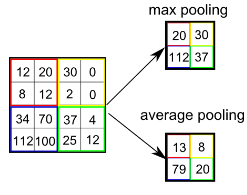
\includegraphics[width=0.2\linewidth]{chapters/neural/images/пуллинг.png}

\label{fig:pulling}

\end{figure}

\begin{figure}[h]

\centering

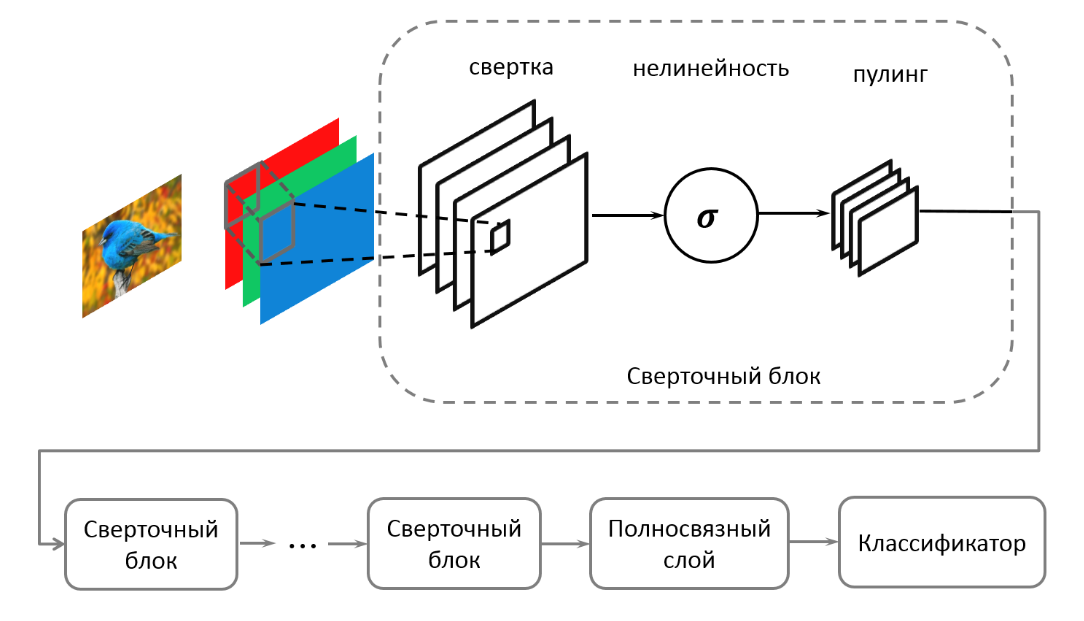
\includegraphics[width=0.8\linewidth]{chapters/neural/images/1CNN.png}

\label{fig:one_cnn}

\end{figure}

Свёрточная сеть обучается извлечению признаков

Чем выше слой, тем более крупные и сложные элементы изображений он способен распознавать

\newpage
\subsection{Приложения CNN.}

Классификация изображений( Свёрточная сеть \textbf{AlexNet} )\\

Распознавание речевых сигналов\\
\begin{figure}[h]

\centering

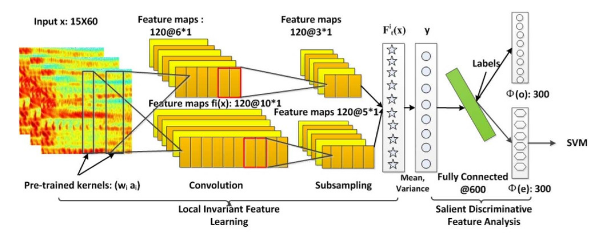
\includegraphics[width=0.8\linewidth]{chapters/neural/images/pic.png}

\label{fig:voice_signals_nn}

\end{figure}

Классификация предложений в тексте:\\
Последовательные слова в тексте представляются векторами с помощью векторных представлений (word2vec и др.)\\

\newpage
\subsection{Обобщение CNN на любые структурированные данные.}
Допустим, каждый объект имеет структуру, заданную графом

\textbf{Свёртка} определяется по локальной окрестности вершины

\textbf{Пулинг} агрегирует векторы вершин локальной окрестности

Такая сеть обучается находить и классифицировать подграфы

\begin{figure}[h]

\centering

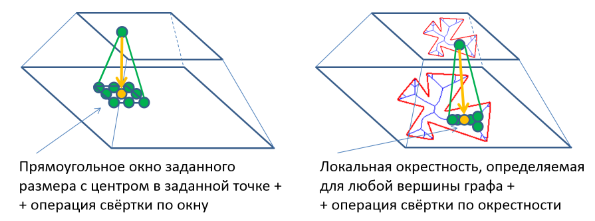
\includegraphics[width=0.8\linewidth]{chapters/neural/images/обобщениеCNN.png}

\label{fig:cnn_generalization}

\end{figure}

\subsection{Задачи}
\textbf{Задача 1}

Дано изображение размером 5x5 пикселей и свёрточное ядро размером 3x3 пикселя\\

\begin{equation*}
\begin{Vmatrix}
1 & 2 & 3 & 0 & 1\\
4 & 5 & 6 & 1 & 0\\
7 & 8 & 9 & 2 & 1\\
0 & 1 & 2 & 3 & 4\\
1 & 0 & 1 & 0 & 1
\end{Vmatrix}
""
\begin{Vmatrix}
1 & 0 & -1\\
1 & 0 & -1\\
1 & 0 & -1
\end{Vmatrix}
\end{equation*}
Необходимо выполнить операцию свёртки\\
\textbf{Решение}

1.Результирующая матрица после свёртки будет размером
$$ (5-3+1) \times (5-3+1) = 3 \times 3 $$.

2. Процесс свёртки:

Для каждого положения свёрточного ядра на изображении вычисляем\\
сумму произведений.

Позиция (0,0):
$
(1 \times 1) + (2 \times 0) + (3 \times -1) + \\
(4 \times 1) + (5 \times 0) + (6 \times -1) + \\
(7 \times 1) + (8 \times 0) + (9 \times -1) = \\
1 + 0 - 3 + 4 + 0 - 6 + 7 + 0 - 9 = -6
$

 Позиция (0,1):
$
(2 \times 1) + (3 \times 0) + (0 \times -1) + \\
(5 \times 1) + (6 \times 0) + (1 \times -1) + \\
(8 \times 1) + (9 \times 0) + (2 \times -1) = \\
2 + 0 + 0 + 5 + 0 - 1 + 8 + 0 - 2 = 12
$

Позиция (0,2):
$
(3 \times 1) + (0 \times 0) + (1 \times -1) + \\
(6 \times 1) + (1 \times 0) + (2 \times -1) + \\
(9 \times 1) + (2 \times 0) + (1 \times -1) = \\
3 + 0 - 1 + 6 + 0 - 2 + 9 + 0 - 1 = 16
$

Позиция (1,0):
$
(4 \times 1) + (5 \times 0) + (6 \times -1) + \\
(7 \times 1) + (8 \times 0) + (9 \times -1) + \\
(0 \times 1) + (1 \times 0) + (2 \times -1) = \\
4 + 0 - 6 + 7 + 0 - 9 + 0 + 0 - 2 = -6
$

Позиция (1,1):
$
(5 \times 1) + (6 \times 0) + (1 \times -1) + \\
(8 \times 1) + (9 \times 0) + (2 \times -1) + \\
(1 \times 1) + (0 \times 0) + (3 \times -1) = \\
5 + 0 - 1 + 8 + 0 - 2 + 1 + 0 - 3 = 8
$

Позиция (1,2):
$
(6 \times 1) + (1 \times 0) + (0 \times -1) + \\
(9 \times 1) + (2 \times 0) + (1 \times -1) + \\
(2 \times 1) + (3 \times 0) + (4 \times -1) = \\
6 + 0 + 0 + 9 + 0 - 1 + 2 + 0 - 4 = 12
$

Позиция (2,0):
$
(7 \times 1) + (8 \times 0) + (9 \times -1) + \\
(0 \times 1) + (1 \times 0) + (2 \times -1) + \\
(1 \times 1) + (0 \times 0) + (3 \times -1) = \\
7 + 0 - 9 + 0 + 0 - 2 + 1 + 0 - 3 = -4
$

Позиция (2,1):
$
(8 \times 1) + (9 \times 0) + (2 \times -1) + \\
(1 \times 1) + (2 \times 0) + (3 \times -1) + \\
(0 \times 1) + (1 \times 0) + (4 \times -1) = \\
8 + 0 - 2 + 1 + 0 - 3 + 0 + 0 - 4 = 0
$

Позиция (2,2):
$
(9 \times 1) + (2 \times 0) + (1 \times -1) + \\
(2 \times 1) + (3 \times 0) + (4 \times -1) + \\
(1 \times 1) + (0 \times 0) + (1 \times -1) = \\
9 + 0 - 1 + 2 + 0 - 4 + 1 + 0 - 1 = 6
$

После выполнения всех операций свёртки\\
мы получаем следующую матрицу:

$$
\begin{Vmatrix}
-6 & 12 & 16 \\
-6 & 8 & 12 \\
-4 & 0 & 6 \\
\end{Vmatrix}
$$

\newpage
\textbf{Задача 2}

Даны изображения продукции с производственной линии.\\
К сожалению, некоторые с дефектами.\\
Предоставьте алгоритм построения CNN для распознавания дефектов на изображениях.

\textbf{Подойдёт такое решение:}

\begin{enumerate}
    \item Создать CNN с тремя свёрточными слоями и двумя pooling-слоями.
    \item Использовать dropout для предотвращения переобучения.
    \item Добавить полносвязный слой перед выходным слоем.
    \item Взять сигмоидный выходной слой для бинарной классификации.
    \item Обучить модель на размеченных изображениях, используя функцию потерь бинарная кросс-энтропия.\end{enumerate}\\

\textbf{Задача 3}

Каковы основные компоненты CNN и их функции?\\
\textbf{Решение:}
\begin{itemize}
    \item Свёрточные слои: применяют свёртку к входным данным, чтобы выделить важные признаки.
    \item Слои подвыборки(Pooling): уменьшают размерность данных, сохраняя наиболее значимую информацию.
    \item Полносвязные слои: используются для окончательной классификации на основе извлечённых признаков.
\end{itemize}

\end{description}


\section*{Оптимальное прореживание нейронных сетей}

\subsection*{Введение}
Прореживание нейронных сетей (англ. optimal brain damage) — метод упрощения структуры регрессионной модели, например, нейронной сети. Основная идея прореживания (англ. pruning) заключается в том, что те элементы модели или те нейроны сети, которые оказывают малое влияние на ошибку аппроксимации, можно исключить из модели без значительного ухудшения качества аппроксимации \cite[VorontsovOptBrainDamage].
Такой подход позволяет достичь следующих целей:
\begin{itemize}
    \item \textbf{Сжатие нейросети.} Уменьшается количество параметров, которые нужно хранить, что важно для устройств с ограниченными ресурсами.
    \item \textbf{Ускорение вычислений.} Меньшее количество параметров требует меньше операций умножения, что ускоряет работу модели.
    \item \textbf{Регуляризация.} Снижение числа параметров уменьшает склонность модели к переобучению, делая её более устойчивой к шуму данных.
    \item \textbf{Повышение качества.} Часто итоговая модель после прореживания показывает лучшие результаты, чем исходная.
    Это связано с тем, что избыточно сложная модель склонна к переобучению, а последовательное исключение избыточных параметров позволяет оптимально адаптировать её сложность к задаче.
\end{itemize}

\subsection*{История метода}
Метод второго порядка был предложен Яном ЛеКуном в 1990 году \cite{lecun1990optimal} и получил название \textit{Optimal Brain Damage}.
На тот момент этот подход был одним из лучших для уменьшения размеров нейронных сетей и улучшения их качества.
Позднее Хассиби и Штурм \cite{hassibi1993optimal} разработали его улучшение \textit{Optimal Brain Surgery}, основываясь на анализе вторых производных. 
Ранее существовали методы нулевого порядка, где исключались элементы с малыми весами \cite{mozer1989skeletonization}.
В 1990 году А. Н. Горбань предложил метод, использующий первые производные, что позволило обойтись без вычисления вторых производных. 
Этот подход получил название \textit{контрастирование нейронных сетей}. Е. М. Миркес развил идеи Горбаня, создав библиотеку функций и язык описания для проекта «Идеального нейрокомпьютера».

Впоследствии появились более современные методы, например Dropout, $L_2$-регуляризация и другие, которые вытеснили этот подход из основного арсенала.
Тем не менее, метод прореживания всё ещё может быть полезным инструментом, особенно в ситуациях, требующих компактности модели.

\subsection*{Математическая постановка задачи}
Рассмотрим регрессионную модель 
\[
y_n = f(\mathbf{w}, \mathbf{x}_n) + \nu,
\]
где $\mathbf{w} \in \mathbb{R}^d$ — вектор параметров, $\mathbf{x}_n \in \mathbb{R}^p$ — вектор независимых переменных, $y_n \in \mathbb{R}$ — зависимая переменная, $\nu$ — случайная ошибка. 

Задана выборка $D = \{(\mathbf{x}_n, y_n)\}_{n=1}^N$. Для минимизации функции ошибки 
\[
E_D(\mathbf{w}) = \sum_{n=1}^N \ell(y_n, f(\mathbf{w}, \mathbf{x}_n)),
\]
где $\ell(\cdot, \cdot)$ — функция потерь, требуется найти $\mathbf{w}^{MP} = \arg\min_{\mathbf{w}} E_D(\mathbf{w})$. 

\subsection*{Прореживание параметров}
Цель метода — исключение параметров $w_i$, которые оказывают наименьшее влияние на ошибку $E_D$.
Для этого используется квадратичная аппроксимация $E_D$ в окрестности $\mathbf{w}^{MP}$:
\[
E_D(\mathbf{w} + \Delta\mathbf{w}) \approx E_D(\mathbf{w}^{MP}) + \frac{1}{2} \Delta\mathbf{w}^T H \Delta\mathbf{w},
\]
где $H = \nabla^2_{\mathbf{w}} E_D(\mathbf{w}^{MP})$ — матрица Гессе.

Исключение параметра $w_i$ эквивалентно наложению ограничения $\Delta w_i + w_i = 0$.
Для выполнения данного условия минимизируется функция:
\[
\Delta E_D = \frac{1}{2} \Delta\mathbf{w}^T H \Delta\mathbf{w},
\]
при ограничении $\mathbf{e}_i^T \Delta\mathbf{w} + w_i = 0$, где $\mathbf{e}_i$ — единичный вектор с $i$-м элементом, равным $1$. 

\subsection*{Оптимизация}
Используем метод множителей Лагранжа для минимизации:
\[
S = \frac{1}{2} \Delta\mathbf{w}^T H \Delta\mathbf{w} - \lambda (\mathbf{e}_i^T \Delta\mathbf{w} + w_i).
\]
Дифференцируя $S$ по $\Delta\mathbf{w}$ и $\lambda$ и приравнивая производные к нулю, получаем:
\[
\Delta\mathbf{w} = -\frac{w_i}{[H^{-1}]_{ii}} H^{-1} \mathbf{e}_i.
\]
Подставляя это выражение в $\Delta E_D$, находим:
\[
L_i = \frac{w_i^2}{2 [H^{-1}]_{ii}}.
\]
Параметр $i$, минимизирующий $L_i$, выбирается для исключения.

\subsection*{Итеративный процесс прореживания}
Вышенаписанный процесс можно повторять несколько раз для повышения эффиктивности модели:
\begin{enumerate}
    \item Определяется вес, который оказывает минимальное влияние на ошибку, и он исключается из модели.
    Удаление выполняется до тех пор, пока ошибка не превышает заданный порог.
    \item После удаления части параметров модель дообучается, чтобы восстановить её качество.
    \item Процесс повторяется, пока не будет достигнута желаемая компактность или качество модели или пока не пройдет заданное число итераций.
\end{enumerate}

\subsection*{Задачи}
\begin{task}
Выпишите Лагранжиан для решения задачи нахождения веса, зануление которого ведет к минимальной ошибке для методов 3 и 4 порядков. Попробуйте решить эту оптимизационную задачу.
\end{task}

\begin{task}
Мы раскладываем функции ошибки до второй производной, хотя приращение $\Delta w_i = -w_i$ может быть достаточно большим. Оцените применимость данного метода в зависимости от величины весов $w_i$.
\end{task}

\begin{task}
Рассчитайте $L_i$ для модели, в которой $H = \begin{bmatrix} 4 & 2 \\ 2 & 3 \end{bmatrix}$, $w = \begin{bmatrix} 1 \\ -2 \end{bmatrix}$.
\end{task}

\section{Batch normalization}

\subsection{Введение}
В основе Batch Normalization лежит решение проблемы «внутреннего ковариационного сдвига» (Internal Covariate Shift). Этот термин описывает явление, при котором распределение входных данных каждого слоя нейронной сети меняется в процессе обучения, из-за чего сети становится сложнее обучать. Это происходит из-за того, что параметры предыдущих слоев изменяются во время обучения, влияя на данные текущего слоя.

Batch Normalization решает эту проблему, нормализуя выход каждого слоя. Нормализация заключается в преобразовании входных данных каждого слоя таким образом, чтобы среднее значение было приближено к нулю, а стандартное отклонение — к единице. Это делает сеть менее чувствительной к масштабу входных данных и улучшает общую стабильность процесса обучения.

Причина популярности batch normalization заключается в значительном ускорении обучения нейронных сетей и в улучшении их сходимости в целом. Его использование гарантирует, что каждая компонента представления на выходе будет иметь контролируемое среднее и дисперсию.

\subsection{Алгоритм}
Сперва идёт слой batch normalization, на котором текущий батч приводится к нулевому среднему и единичной дисперсии, где $\mu$ и $\sigma^2$ - среднее и дисперсия признаков по обрабатываемому батчу, $\varepsilon$ - гиперпараметр слоя, служащий для численной устойчивости.

\[X^{k+1} = \frac{X^k - \mu}{\sqrt{\sigma^2 + \varepsilon}}\]

Далее идёт слой channelwise scaling, который позволяет выучить оптимальное шкалирование для всех признаков $X^{k+2}$. Где $beta$ и $\gamma$ - обучаемые параметры, позволяющие настраивать в ходе обучения оптимальные значения матожидания и дисперсии выходного слоя.

\[X^{k+2} = \beta X^{k+1} + \gamma \]

В ходе предсказания мы используем $\mu_*$ $\sigma_*^2$, полученные в ходе обучения как скользящее среднее всех средних и дисперсий. 

\subsection{Задачи}

\subsubsection*{Задача 1}
Рассмотрим ситуацию: у вас есть небольшой набор данных, и мини-батчи содержат только по 2-3 образца. Какие проблемы могут возникнуть при использовании Batch Normalization в таких условиях? Какие методы можно использовать для решения этих проблем?

\subsubsection*{Задача 2}
Как параметры скользящих статистик влияют на работу модели?

\subsubsection*{Задача 3}
Почему нельзя использовать статистики конкретного батча во время предсказания


\section{Методы оптимизации с использованием Autograd: SGD, Adam, RMSProp}

\subsection{Автоматическое дифференцирование с Autograd}

Autograd \textendash{} это инструмент для автоматического дифференцирования, который позволяет автоматически вычислять градиенты функций. В контексте методов оптимизации, Autograd упрощает процесс нахождения производных для сложных функций потерь. Благодаря Autograd, пользователю не нужно вручную выводить градиенты \textendash{} они вычисляются программно с использованием обратного распространения (backpropagation).

Autograd используется во многих популярных библиотеках, таких как \texttt{PyTorch} и \texttt{JAX}. На семинарах были продемонстрированы примеры использования Autograd для автоматического вычисления градиентов при оптимизации нейронных сетей.

\subsubsection{Пример использования Autograd}

Предположим, у нас есть функция потерь $L(\theta) = (\theta^2 + 3\theta + 2)$. С помощью Autograd можно вычислить градиент этой функции по параметру $\theta$:

\begin{verbatim}
import autograd.numpy as np
from autograd import grad

def loss(theta):
    return theta**2 + 3 * theta + 2

grad_loss = grad(loss)
print(grad_loss(1.0))  # Выводит 5.0
\end{verbatim}

\subsection{Стохастический градиентный спуск (SGD)}

Стохастический градиентный спуск (SGD) представляет собой метод оптимизации, который используется для минимизации функции потерь $L(\theta)$, где $\theta$ \textendash{} параметры модели. На каждом шаге обновления параметров SGD использует оценку градиента по одному или нескольким случайно выбранным объектам:

\begin{equation}
\theta_{t+1} = \theta_t - \eta \nabla_\theta L_i(\theta_t),
\end{equation}

где:
\begin{itemize}
    \item $\theta_t$ \textendash{} параметры на шаге $t$;
    \item $\eta$ \textendash{} коэффициент обучения;
    \item $\nabla_\theta L_i(\theta_t)$ \textendash{} градиент функции потерь по $i$-му примеру на шаге $t$.
\end{itemize}

SGD часто используется благодаря своей простоте, но он может быть неустойчивым и медленным при выборе неподходящего коэффициента обучения.

\subsection{RMSProp}

Метод RMSProp (Root Mean Square Propagation) предназначен для адаптивного изменения шага обучения. В отличие от SGD, RMSProp учитывает среднеквадратичное значение градиентов для каждого параметра. Формулы для обновления параметров имеют вид:

\begin{align}
    g_t &= \nabla_\theta L_i(\theta_t), \\
    v_t &= \gamma v_{t-1} + (1 - \gamma) g_t^2, \\
    \theta_{t+1} &= \theta_t - \frac{\eta}{\sqrt{v_t + \epsilon}} g_t,
\end{align}

где:
\begin{itemize}
    \item $v_t$ \textendash{} скользящее среднее квадратов градиентов;
    \item $\gamma$ \textendash{} коэффициент сглаживания (обычно $0.9$);
    \item $\epsilon$ \textendash{} небольшая константа для избежания деления на ноль.
\end{itemize}

\subsection{Adam}

Метод Adam (Adaptive Moment Estimation) сочетает идеи из SGD и RMSProp, используя как первую, так и вторую моменты градиентов. Алгоритм Adam вычисляется по следующим формулам:

\begin{align}
    g_t &= \nabla_\theta L_i(\theta_t), \\
    m_t &= \beta_1 m_{t-1} + (1 - \beta_1) g_t, \\
    v_t &= \beta_2 v_{t-1} + (1 - \beta_2) g_t^2, \\
    \hat{m}_t &= \frac{m_t}{1 - \beta_1^t}, \\
    \hat{v}_t &= \frac{v_t}{1 - \beta_2^t}, \\
    \theta_{t+1} &= \theta_t - \frac{\eta}{\sqrt{\hat{v}_t} + \epsilon} \hat{m}_t,
\end{align}

где:
\begin{itemize}
    \item $m_t$ \textendash{} скользящее среднее градиентов (первая производная);
    \item $v_t$ \textendash{} скользящее среднее квадратов градиентов (вторая производная);
    \item $\beta_1$ и $\beta_2$ \textendash{} коэффициенты экспоненциального сглаживания (обычно $\beta_1 = 0.9$ и $\beta_2 = 0.999$);
    \item $\hat{m}_t$ и $\hat{v}_t$ \textendash{} корректированные моменты с учётом смещения;
    \item $\eta$ \textendash{} шаг обучения.
\end{itemize}

\subsection{Задачи}

\subsubsection*{Задача 1}
Рассмотрим функцию потерь $L(\theta) = \theta^2$. Используя SGD с шагом обучения $\eta = 0.1$, выполните два шага оптимизации, начиная с $\theta_0 = 1$. Найдите $\theta_1$ и $\theta_2$.

\textbf{Решение:}
\begin{align*}
    \nabla_\theta L(\theta_0) &= 2 \cdot \theta_0 = 2 \cdot 1 = 2, \\
    \theta_1 &= \theta_0 - 0.1 \cdot 2 = 1 - 0.2 = 0.8, \\
    \nabla_\theta L(\theta_1) &= 2 \cdot 0.8 = 1.6, \\
    \theta_2 &= \theta_1 - 0.1 \cdot 1.6 = 0.8 - 0.16 = 0.64.
\end{align*}

\subsubsection*{Задача 2}
Покажите, что в RMSProp, если градиент на каждом шаге постоянен и равен $g$, значение $v_t$ стремится к $g^2$ при $t \to \infty$.

\textbf{Решение:}
\begin{align*}
    v_t &= \gamma v_{t-1} + (1 - \gamma) g^2.
\end{align*}

В установившемся режиме $v_t = v_{t-1} = v$, поэтому:
\begin{align*}
    v &= \gamma v + (1 - \gamma) g^2, \\
    v (1 - \gamma) &= (1 - \gamma) g^2, \\
    v &= g^2.
\end{align*}

\subsubsection*{Задача 3}
Докажите, что для Adam корректированные моменты $\hat{m}_t$ и $\hat{v}_t$ стремятся к $m_t$ и $v_t$ соответственно при $t \to \infty$.

\textbf{Решение:}
\begin{itemize}
    \item $\hat{m}_t = \frac{m_t}{1 - \beta_1^t}$. При $t \to \infty$, $\beta_1^t \to 0$, поэтому $1 - \beta_1^t \to 1$ и $\hat{m}_t \to m_t$.
    \item Аналогично, $\hat{v}_t = \frac{v_t}{1 - \beta_2^t}$, и при $t \to \infty$, $\hat{v}_t \to v_t$.
\end{itemize}

\section{LSTM и GRU}

\subsection{LSTM. Основная идея}

\begin{figure}[h]
	\centering
	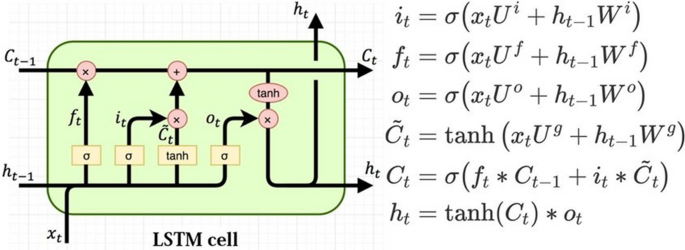
\includegraphics[width=0.6\linewidth]{chapters/neural/images/lstm.png}
	\caption{Схема LSTM}
	\label{img:lstm}
\end{figure}
Основная идея LSTM~\cite{hochreiter1997long} --- использование механизма \textbf{ячейки памяти} и набора \textbf{затворов (gates)}, которые регулируют, какая часть информации из предыдущих шагов будет запоминаться, забываться и выводиться на выход. Это позволяет LSTM ``удерживать'' важную информацию на более длинных промежутках.

\subsection{Структура LSTM-ячейки}
В классической LSTM-ячейке три затвора:
\begin{enumerate}
    \item \textbf{Forget gate} (затвор забывания) управляет тем, какая часть предыдущего состояния памяти $C_{t-1}$ будет \textit{забыта}.
    \item \textbf{Input gate} (затвор записи) определяет, какая часть нового кандидата состояния $\tilde{C}_t$ попадёт в текущее состояние памяти.
    \item \textbf{Output gate} (затвор выхода) определяет, какая часть текущего состояния памяти $C_t$ будет подана на выход $h_t$.
\end{enumerate}

Типичные формулы (безbias-термов):
\[
f_t = \sigma(W_f \cdot [h_{t-1}, x_t]), \quad
i_t = \sigma(W_i \cdot [h_{t-1}, x_t]), \quad
\tilde{C}_t = \tanh(W_C \cdot [h_{t-1}, x_t]),
\]
\[
C_t = f_t \odot C_{t-1} + i_t \odot \tilde{C}_t,
\]
\[
o_t = \sigma(W_o \cdot [h_{t-1}, x_t]), \quad
h_t = o_t \odot \tanh(C_t).
\]

\subsection{Продвинутые моменты LSTM}
\begin{itemize}
    \item \textbf{Bidirectional LSTM}: двунаправленная архитектура для учёта контекста слева и справа.
    \item \textbf{Stacked LSTM}: многослойные (глубокие) LSTM для повышения выразительности.
    \item \textbf{Dropout и Recurrent Dropout}: регуляризация занулением нейронов в связях.
    \item \textbf{Attention Mechanisms}: совмещение с механизмом внимания (Attention) для более гибкого «фокуса» на нужных шагах входной последовательности.
\end{itemize}

\subsection{Архитектура GRU}

\begin{figure}[h]
	\centering
	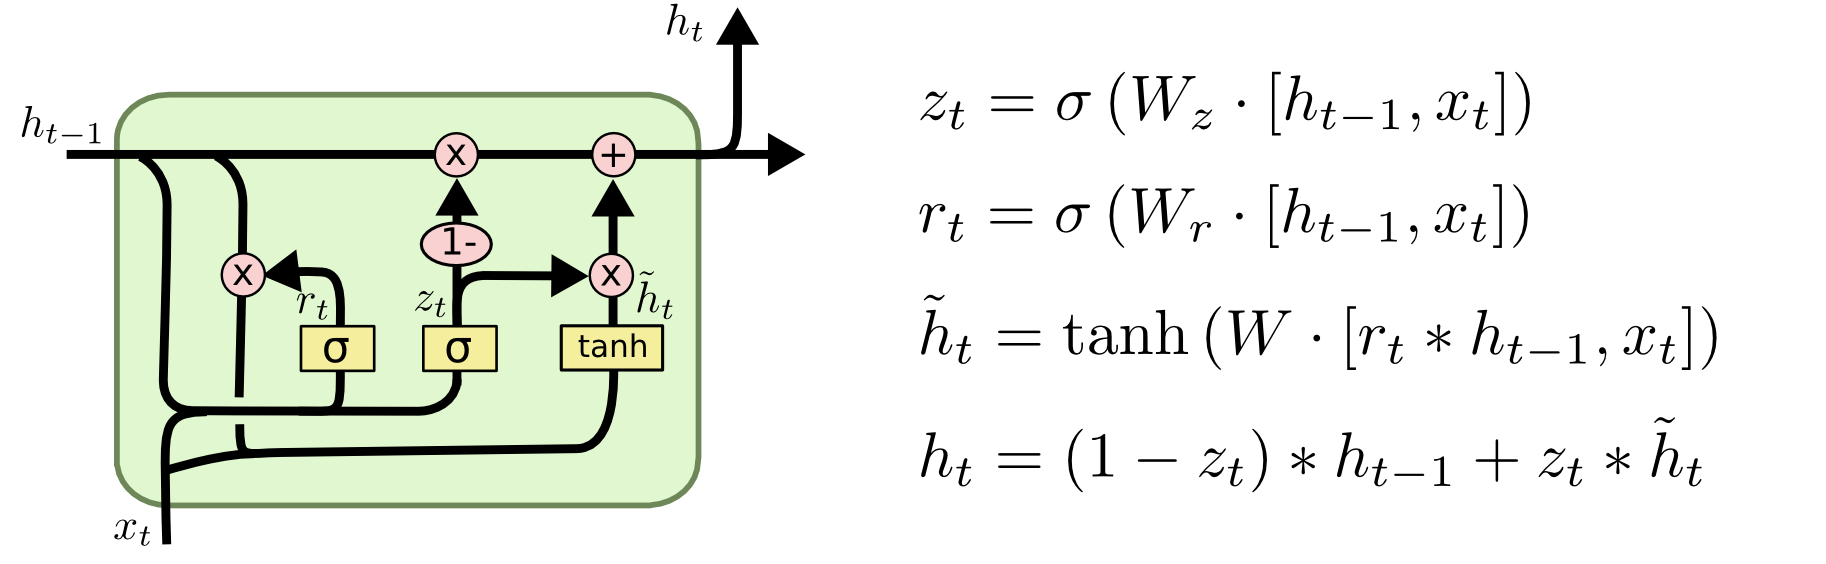
\includegraphics[width=0.6\linewidth]{chapters/neural/images/gru.png}
	\caption{Схема GRU}
	\label{img:gru}
\end{figure}
GRU (Gated Recurrent Unit) была предложена в работе~\cite{cho2014properties} как упрощение по сравнению с LSTM: используется всего два затвора (update и reset), что уменьшает число параметров модели.

\subsection{Структура GRU-ячейки}
\begin{enumerate}
    \item \textbf{Update gate} $z_t$ управляет тем, сколько информации из предыдущего выхода $h_{t-1}$ перенести в новое состояние.
    \item \textbf{Reset gate} $r_t$ определяет, сколько ``старой'' информации нужно сбросить перед вычислением текущего кандидата.
\end{enumerate}

Основные формулы:
\[
z_t = \sigma(W_z \cdot [h_{t-1}, x_t]), \quad
r_t = \sigma(W_r \cdot [h_{t-1}, x_t]),
\]
\[
\tilde{h}_t = \tanh \bigl(W_h \cdot [r_t \odot h_{t-1}, x_t]\bigr),
\]
\[
h_t = (1 - z_t)\odot h_{t-1} + z_t \odot \tilde{h}_t.
\]

\subsection{Преимущества GRU}
\begin{itemize}
    \item Меньше параметров по сравнению с LSTM, что может ускорять обучение.
    \item Часто качество на задачах NLP и временных рядах сопоставимо с LSTM.
\end{itemize}

\subsection{Продвинутые моменты GRU}
\begin{itemize}
    \item \textbf{Layer Normalization / BatchNorm}: нормализация на выходе или по слоям помогает стабилизировать обучение.
    \item \textbf{Residual/Skip Connections}: добавляются короткие связи для улучшения обратного распространения ошибки.
    \item \textbf{Bidirectional GRU}: аналогично двунаправленным LSTM, учитываем контекст с двух сторон.
\end{itemize}

\subsection{Сравнение LSTM и GRU}
\begin{itemize}
    \item LSTM имеет более гибкую структуру (три затвора, отдельное состояние $C_t$), но и больше параметров.
    \item GRU проще, часто обучается быстрее и даёт сравнимое качество.
\end{itemize}


\subsection{Теоретическая Задача 1: Анализ взрывающих и затухающих градиентов}
Объясните, почему в классической RNN (без затворов) возникает проблема затухающих и взрывающих градиентов при обучении на длинных последовательностях. Как архитектуры LSTM и GRU помогают смягчить эту проблему?

\begin{itemize}
    \item \textbf{Классическая RNN} использует повторяющиеся умножения весовых матриц на каждом временном шаге. Для длинных цепочек такие последовательные умножения могут привести к экспоненциальному затуханию или экспоненциальному росту (взрыв градиентов), поскольку собственные значения матриц многократно перемножаются.
    \item \textbf{LSTM и GRU} вводят механизмы затворов и явные пути прямой передачи градиента (``гейтированные'' или ``прямые'' связи через состояние), что существенно стабилизирует процесс обучения. Ячейка памяти LSTM (и аналогичная структура в GRU) создаёт путь, по которому градиент может проходить без постоянного перемножения на матрицу весов. Таким образом, модели меньше страдают от затухания или взрыва.
\end{itemize}

\subsection{Теоретическая Задача 2: Сравнение количества параметров в LSTM и GRU}
Предположим, что размерность входа равна $d$, а размер скрытого состояния равен $h$. Сравните (количественно) число обучаемых параметров в одной LSTM-ячейке и одной GRU-ячейке. Объясните, как это влияет на время обучения и возможность переобучения?

\begin{itemize}
    \item \textbf{LSTM} имеет 4 вычислительных ``ветви'' (forget, input, candidate, output), каждая включает матрицу весов для входа $W_{*}^{(x)}$ и для предыдущего скрытого состояния $W_{*}^{(h)}$, а также соответствующие bias. Итого для LSTM:
    \[
    \text{Параметры в LSTM} \approx 4 \cdot (d \cdot h + h \cdot h + h)
    \]
    \item \textbf{GRU} имеет 3 ветви (update, reset, candidate), что даёт формулу:
    \[
    \text{Параметры в GRU} \approx 3 \cdot (d \cdot h + h \cdot h + h)
    \]
    \item Таким образом, GRU имеет меньше параметров, что может приводить к более быстрой сходимости и меньшей склонности к переобучению (но и менее ``гибкой'' архитектуре в некоторых случаях).
\end{itemize}

\subsection{Теоретическая Задача 3: Пределы LSTM/GRU при очень длинных зависимостях}

Поясните, в каких случаях даже LSTM или GRU могут не справляться с очень длинными зависимостями? Предложите, какие механизмы или архитектуры способны улучшить качество работы с подобными зависимостями.

\begin{itemize}
    \item \textbf{Очень длинные зависимости}: даже с механизмами затворов для очень больших длин (например, сотни или тысячи временных шагов) LSTM/GRU могут всё ещё сталкиваться с трудностями в запоминании самых первых шагов. 
    \item \textbf{Mechanisms/архитектуры}: 
    \begin{itemize}
        \item \textbf{Attention} (применение в Encoder-Decoder архитектурах). Позволяет модели ``обращаться'' к нужным шагам напрямую, минуя долгую цепочку рекуррентных состояний.
        \item \textbf{Transformers}: полностью отказываются от рекуррентной структуры и используют механизм внимания (self-attention), что улучшает способность моделировать дальние зависимости.
        \item \textbf{Memory-augmented networks} (Neural Turing Machines, Memory Networks): явное внешнее хранилище.
    \end{itemize}
\end{itemize} 

\section{KAN как альтернативная базовая архитектура}
\subsection{Теорема Коллмогорова Арнольда}

В области машинного обучения многослойные персептроны (MLP) традиционно считаются универсальными аппроксиматорами функций. Однако существует менее известный, но не менее важный математический результат - теорема Колмогорова-Арнольда, которая предлагает альтернативный подход к представлению многомерных функций.
Теорема Колмогорова-Арнольда, доказанная в 1957 году, утверждает, что любая непрерывная функция нескольких переменных может быть представлена как суперпозиция непрерывных функций одной переменной и операции сложения. Формально это можно записать следующим образом:
\[
f(x_1, ..., x_n) = \sum_{q=1}^{2n+1} \Phi_q \left(\sum_{p=1}^n \phi_{q,p}(x_p)\right)
\]
где $\phi_{q,p}$ и $\Phi_q $ - непрерывные функции одной переменной.

Долгое время теорема Колмогорова-Арнольда считалась преимущественно теоретическим результатом без практического применения. Основная причина заключалась в том, что функции $\phi_{q,p}$ и $\Phi_q$ могут быть очень сложными и даже разрывными, что делает их непрактичными для численной реализации.

\subsubsection{Теоретическая задача 1: представление Колмогорова-Арнольда}
Приведите функцию $ f(x,y,z) = \frac{x^y}{z} $ в виде представления Колмогорова-Арнольда

\textbf{Решение:}
\[
f(x,y,z) = \frac{x^y}{z} = \exp(\exp(\log y + \log \log x) + (-\log z))
\]
\[
\Phi_1 = \exp
\]
\[
\phi_{1, 1} = \exp\log(y)
\]
\[
\phi_{1, 2} = \log\log(y)
\]
\[
\phi_{1, 3} = -\log z
\]

\subsection{Kolmogorov-Arnold Networks (KAN)}

Теорема Колмогорова-Арнольда вдохновила создание нового класса нейронных сетей - сетей Колмогорова-Арнольда (KAN), которые предлагают альтернативу традиционным многослойным персептронам. В то время как MLP используют фиксированные функции активации на узлах ("нейронах"), KAN размещает обучаемые функции активации на рёбрах ("весах") и реализует их с помощью B-сплайнов.
B-сплайны представляют собой кусочно-полиномиальные функции, обладающие рядом важных свойств:
\begin{itemize}
    \item Локальность: изменение одного контрольного узла влияет только на ограниченную область функции
    \item Гладкость: B-сплайны обеспечивают заданную степень непрерывности производных
    \item Компактность: эффективное представление сложных функций с небольшим числом параметров
\end{itemize}

Формально, слой KAN с входной размерностью $n_{in}$ и выходной размерностью $n_{out}$ можно определить как матрицу одномерных функций:
\[
\Phi(X) = {\phi_{q,p}}, p = 1,2,\ldots,n_{in}, q = 1,2,\ldots,n_{out}
\]
где каждая функция $\phi_{q,p}$ параметризована как B-сплайн с обучаемыми коэффициентами.

Главным отличием от исходной теоремы в KAN является уход от фиксированной глубины. Полная нейронная сеть представляет из себя композицию слоёв, то есть последовательное применение функциональных матриц:
\[
KAN(X) = \Phi_n(\Phi_{n - 1}( ...\Phi_2(\Phi_1(X))...))
\]

Исследования показывают, что KAN могут достигать сравнимой или лучшей точности по сравнению с более крупными MLP при использовании значительно меньшего количества параметров. Например, для решения дифференциальных уравнений в частных производных двухслойная KAN шириной 10 может быть в 100 раз точнее и в 100 раз эффективнее по параметрам, чем четырехслойная MLP шириной 100.

\subsubsection{Теоретическая задача 2: сети Колмогорова-Арнольда}
Покажите, как использовать обратное распространениие ошибки для обучения KAN.

\textbf{Решение:}

Использование B-сплайна в определении слоя затрудняет прямое применение обратного распространения ошибки, так как его производная в каждой точке заранее неизвестна. Однако каждый B-сплайн можно заменить на скрытый слой из перцептронов с одним входом и разными функциями активации, соответствующими базисным функциям сплайна, производные которых известны заранее. Таким образом KAN сводится к традиционной нейронной сети.

\subsection{КАН для обучения без учителя}

Сети Колмогорова-Арнольда могут быть эффективно адаптированы для задач обучения без учителя, что открывает новые возможности для анализа данных и научных открытий. В отличие от традиционного применения в задачах обучения с учителем, KAN для обучения без учителя фокусируются на поиске скрытых зависимостей в данных без явного указания целевых переменных.
Основная идея заключается в преобразовании задачи обучения без учителя в специальную форму обучения с учителем. Пусть имеется набор признаков $(x_1, x_2, ..., x_d)$, среди которых предполагается наличие функциональных зависимостей. Цель состоит в поиске нетривиальной функции $f$, такой что:
\[
f(x_1, x_2, ..., x_d) \approx 0
\]

Для решения этой задачи используется контрастивный подход, где определяются:
Позитивные примеры: реальные наборы признаков
Негативные примеры: наборы признаков с случайной перестановкой значений

KAN обучается различать эти два класса примеров, используя специальную модификацию архитектуры с гауссовой функцией активации в последнем слое:
\[
KAN_{unsupervised}(X) = \delta (KAN(X)), \text{ где } \delta(x) = \exp(-\frac{x^2}{2w^2})
\]
Такой подход позволяет KAN автоматически обнаруживать нетривиальные зависимости в данных. Например, в физических экспериментах сеть может выявлять фундаментальные законы природы, анализируя только измеренные величины.

\subsubsection{Теоретическая задача 3: KAN без учителя}
Какой датасет и какая архитектура KAN нужна для переоткрытия второго закона Ньютона?

\textbf{Решение:}

Набор данных должен содержать следующие измерения:
\begin{itemize}
    \item массы тел (m)
    \item приложенных сил (F)
    \item наблюдаемых ускорений (a)
\end{itemize}

Выражение меняется на:
\[
F=ma\rightarrow F-ma=0
\]
Далее представим это выражение в виде KAN:
\[
KAN(F, m, a) = \delta\left( F-\exp\left( \log m + \log a \right) \right),
\]
\[
\text{ где } \exp, \log \text{ - B-сплайны, определяемые во время обучения}
\]
Для обучения настоящие данные будут иметь целевую переменную равную 1, а случайно созданные - 0. Полученные в результате обучения функции позволят получить правильный вид закона.



\begin{thebibliography}{99}
\bibitem{hochreiter1997long} S.~Hochreiter, J.~Schmidhuber, \textit{Long short-term memory.} Neural Computation, 9(8), 1735--1780, 1997.
\bibitem{cho2014properties} K.~Cho, B.~van Merrienboer, D.~Bahdanau, Y.~Bengio, \textit{On the properties of neural machine translation: Encoder-decoder approaches.} arXiv preprint arXiv:1409.1259, 2014.
\end{thebibliography}

\section*{Быстрые методы стохастического градиента: Поляка и Нестерова}

Методы ускорения градиентного спуска применяются для уменьшения количества итераций, необходимых для достижения минимума функции потерь. Два важных метода для ускорения сходимости — это метод накопления инерции (Momentum) Поляка и метод ускоренного градиента Нестерова.


\subsection*{Метод Поляка (Momentum)}

Метод Поляка использует понятие \textit{накопленной скорости} для сглаживания обновления параметров и уменьшения колебаний. Вместо прямого шага в направлении градиента, метод учитывает предыдущие обновления. Формулы метода:

\begin{equation*}
\begin{aligned}
    v &:= \gamma v + (1 - \gamma) \nabla \mathcal{L}(w, x_i), \\
    w &:= w - \eta v,
\end{aligned}
\end{equation*}
где $\gamma \in [0, 1)$ — коэффициент импульса, $\eta$ — шаг обучения, $\nabla \mathcal{L}(w, x_i)$ — градиент функции потерь для $x_i$, $v$ — накопленная скорость.

Таким образом, метод Поляка комбинирует текущий градиент с предыдущими направлениями движения, что позволяет "разгоняться" в одном направлении и сглаживать траекторию на плоских участках.

\subsection*{Метод Нестерова (Nesterov Accelerated Gradient, NAG)}

Метод Нестерова представляет собой модификацию метода Поляка, где используется идея предварительного "предсказания" положения параметров. Основное отличие в том, что градиент рассчитывается не в текущей точке, а в точке, смещённой в направлении скорости. Формулы обновления параметров:
\begin{equation*}
\begin{aligned}
    v &:= \gamma v + (1 - \gamma) \nabla \mathcal{L}(w - \eta \gamma v, x_i), \\
    w &:= w - \eta v.
\end{aligned}
\end{equation*}

"Заглядывание вперёд" в направлении текущей скорости позволяет более точно учитывать геометрию функции и улучшать сходимость. Это позволяет методу Нестерова минимизировать колебания и снижать избыточные шаги в направлении градиента.

\subsection*{Графическое объяснение методов}

\begin{figure}[h!]
    \centering
    \begin{minipage}[t]{0.45\textwidth}
        \centering
        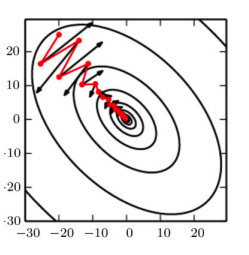
\includegraphics[width=0.9\textwidth]{chapters/neural/images/polyak.png}
        \\[0.5em]
        Рис. 1: Метод Поляка (Momentum)
    \end{minipage}%
    \hfill
    \begin{minipage}[t]{0.45\textwidth}
        \centering
        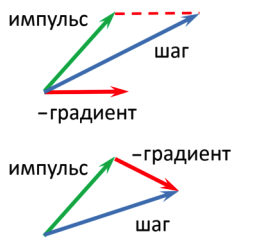
\includegraphics[width=0.9\textwidth]{chapters/neural/images/nesterov.png}
        \\[0.5em]
        Рис. 2: Метод Нестерова (NAG)
    \end{minipage}
\end{figure}

\begin{itemize}
    \item На левом рисунке показано, как метод Поляка сглаживает путь оптимизации за счёт накопленного импульса.
    \item На правом рисунке метод Нестерова использует "предсказание" положения параметров, что приводит к более оптимальному шагу.
\end{itemize}

\subsection*{Сравнение методов}
    \item - Метод Поляка прост в реализации и хорошо работает на негладких функциях.

    \item - Метод Нестерова обеспечивает более высокую скорость сходимости благодаря использованию информации о кривизне.

    \item - Оба метода легко интегрируются в современные алгоритмы оптимизации, такие как Adam и RMSProp.

\subsection*{Задача 1}
Рассмотрим функцию
\[
f(w) = w^2.
\]
Примените метод градиентного спуска с импульсом Поляка для минимизации этой функции. Шаг обучения $\eta = 0.1$, коэффициент импульса $\gamma = 0.9$, начальная точка $w_0 = 5$. Выполните три итерации.

\textbf{Решение:}

\[
v_t = \gamma v_{t-1} + (1 - \gamma) \nabla f(w_t), \quad w_{t+1} = w_t - \eta v_t,
\]
где $v_t$ — накопленная скорость, $\nabla f(w_t)$ — градиент функции $f(w) = w^2$, а $\eta$ — шаг обучения.

1.
   \[
   w_0 = 5, \quad v_0 = 0, \quad \nabla f(w_0) = 2w_0 = 10.
   \]
   \[
   v_1 = 0.9 \cdot 0 + (1 - 0.9) \cdot 10 = 1, \quad w_1 = 5 - 0.1 \cdot 1 = 4.9.
   \]

2.
   \[
   w_1 = 4.9, \quad \nabla f(w_1) = 9.8.
   \]
   \[
   v_2 = 0.9 \cdot 1 + (1 - 0.9) \cdot 9.8 = 1.88, \quad w_2 = 4.9 - 0.1 \cdot 1.88 = 4.712.
   \]

3.
   \[
   w_2 = 4.712, \quad \nabla f(w_2) = 9.424.
   \]
   \[
   v_3 = 0.9 \cdot 1.88 + (1 - 0.9) \cdot 9.424 = 2.634, \quad w_3 = 4.712 - 0.1 \cdot 2.634 = 4.448.
   \]

\textbf{Ответ:} после трёх итераций метода Поляка значение параметра $w$ уменьшилось с 5 до $4.448$ - он движется в сторону минимума функции $f(w) = w^2$.

\subsection*{Задача 2}
Для функции 
\begin{equation*}
    f(w) = (w - 3)^2 + 7
\end{equation*}
выполните две итерации метода Нестерова с параметрами $\eta = 0.2$ и $\gamma = 0.8$, начиная с $w = -1$. Найдите значения $w$ после каждой итерации.

\textbf{Решение:}
\begin{equation*}
    v_k = \gamma v_{k-1} + (1 - \gamma) \nabla f(w_k - \eta \gamma v_{k-1}), \quad w_{k+1} = w_k - \eta v_k.
\end{equation*}
1.
\[
   w_0 = -1, \quad v_0 = 0, \quad \nabla f(-1) = 2(-1 - 3) = -8.
\]
\[ v_1 = 0.8 \cdot 0 + 0.2 \cdot (-8) = -1.6, \quad w_1 = -1 - 0.2 \cdot (-1.6) = -0.68. \]
2. 
\[
   w_1 = -0.68, \quad v_1 = -1.6, \quad \nabla f(-0.68 - 0.2 \cdot 0.8 \cdot (-1.6)) = -6.848.
\]
\[ v_2 = 0.8 \cdot (-1.6) + 0.2 \cdot (-6.848) = -2.08, \quad w_2 = -0.68 - 0.2 \cdot (-2.08) = -0.272. \]

\textbf{Ответ:} после двух итераций значение $w$ изменилось с $-1$ до $-0.272$.

\subsection*{Задача 3}
Рассмотрим функцию:  
 \item\( f_1(w) = 10w_1^2 + w_2^2 \) (вытянутая квадратичная функция)   

Предположим, что для минимизации используется либо метод Поляка (Momentum), либо метод Нестерова (NAG).  
\item Начальная точка: \( w_0 = (10, 5) \),  шаг обучения \( \eta = 0.1 \),   коэффициент импульса \( \gamma = 0.9 \).  

Укажите, какой метод будет эффективнее и почему.

\textbf{Решение:}

1. Градиенты в направлении \( w_1 \) (\( \nabla_{w_1} f = 20w_1 \)) гораздо больше, чем в направлении \( w_2 \) (\( \nabla_{w_2} f = 2w_2 \)). Это приводит к "зигзагообразным" траекториям.

2. Начальная точка \( w_0 = (10, 5) \) находится далеко от минимума (\( w^* = (0, 0) \)). Ошибки по каждой координате значительно различаются, что увеличивает влияние масштабирования на скорость сходимости.

Метод Поляка не учитывает \textit{предсказание будущего положения}, поэтому траектория часто оказывается менее оптимальной в условиях вытянутости. Это может привести к увеличению числа итераций.

Метод Нестерова строит обновление на основе "предсказанной" точки \( w_t - \eta \gamma v_t \), заглядывая вперёд в направлении текущей скорости \( v_t \). Для вытянутых функций это даёт два преимущества:

1. Лучшее согласование шага с направлением градиента:  
    метод Нестерова корректирует траекторию, уменьшает зигзагообразность и быстрее приближается к минимуму.

2. Ускорение сходимости по оси с меньшим масштабом:  
   "заглядывание" даёт возможность быстрее компенсировать медленное движение вдоль более плоской оси \( w_2 \).

\textbf{Вывод: } для данной функции \( f_1(w) = 10w_1^2 + w_2^2 \) метод Нестерова (NAG) будет эффективнее, чем метод Поляка (Momentum), который хотя и полезен для сглаживания колебаний, менее адаптивен к вытянутой геометрии задачи, что приводит к более медленной сходимости.

        
    \clearpage
    \chapter{Метрические методы классификации и регрессии}
    \section{Обобщенный метрический классификатор}

\subsection{Гипотеза непрерывности и компактности}

Прежде, чем строить какой-либо обобщенный метрический метод для задачи классификации или регрессии важно подчеркнуть исходные.

Для задачи регрессии предполагается, что зависимость, которую мы восстанавливаем непрерывная. Т.е. "близким" объектам соответсвуют "близкие" ответы.

Для задач классификации предполагается гипотеза компактности в ее бытовом смысле. Классы - это компактные сгустки точек, т.е. "близкие" объекты, как правило, лежат в одном классе.

\subsection{Формализация расстояния}

Теперь ответим на вопрос, а какие объекты считать "близки" в строгом математическом смысле?

Для определения расстояния используются классические метрики вроде:
\begin{itemize}
    \item Евклидовой метрики
        \begin{equation}
            \rho(x, x_i) = \left( \sum_{j=1}^n |x^j - x^j_i|^2 \right)
        \end{equation}
    \item Обобщенной метрики Миновского
        \begin{equation}
            \rho(x, x_i) = \left( \sum_{j=1}^n w_j |x^j - x^j_i|^p \right)^\frac{1}{p}
        \end{equation}
\end{itemize}
$x = (x^1, ... , x^n)$ - вектор признаков соответствующего объекта; \\ 
$w_1, ... w_n$ - обучаемые веса признаков, отвечающие за приведение к общему масштабу, задание степени информативности признаков.

Для произвольного $x \in X$ отранжируем объекты обучающей выборки $x_1, ..., x_l$ следующим образом:
\begin{equation}
    \rho(x, x^{(1)}) \le \rho(x, x^{(2)}) \le ... \le \rho(x, x^{(l)})
\end{equation}
$x^{(i)}$ - $i$-ый сосед объекта $x$ среди объектов обучающей выборки $x_1, ..., x_l$; \\ 
$y^{(i)}$ - ответ на $i$-ом соседе объекта $x$.

\textbf{Метрический алгоритм классификации:}
\begin{equation}
    a(x; X^l) = arg max_{y \in Y} \underbrace{\sum_{i = 1}^l [y^{(i)} = y]w(i ,x)}_{\Gamma_y(x)}
\end{equation}
$w(i, x)$ - вес, степень близости к объекту $x$ его $i$-го соседа, неотрицателен, не возрастает по $i$; \\
$\Gamma_y(x)$ - оценка близости объекта $x$ к классу $y$.

Стоит отметить, что обобщенный метрический алгоритм особенный среди $ML$ алгоритмов. Обычно любой алгоритм формулируется в формате оптимизационной задачи, решая которую находятся параметры модели. В метрическом алгоритме не ставится задача явной оптимизации.

Фактически алгоритму будут различаться тем, как мы выберем вес $w(i, x)$, характеризующий степень близости.

\subsection{Метод k ближайших соседей (nearest neighbours, kNN)}
Если определить вес как $w(i, x) = [i \le k]$, то и получим метод kNN. Фактически для объекта $x$ проходятся по k его ближайшим соседям, объектов какого класса среди них будет больше, такую метку класса и присвоят объекту $x$.

Преимущества метода:
\begin{itemize}
    \item Простота реализации. Никакой оптимизационной задачи рещать не надо.
    \item Единственный гиперпараметр метода $k$ можно оптимизировать с помощью leave-one-out:
    \begin{equation}
        LOO(k, X^l) = \sum_{i = 1}^l \left[ a(x_i; X^l \backslash x_i, k) \neq y_i \right] \Rightarrow \underset{k}{min}
    \end{equation}
\end{itemize}
Недостатки метода:
\begin{itemize}
    \item Возможно неоднозначная классификация, в случае если среди соседей будет равное число объектов двух разных классов.
    \item Не учитываются значения расстояний. Например, пусть $k = 5$. Первые четыре соседа находятся действительно рядом, а пятый где-то далеко и фактически "ближайшим" соседом не является, но будет учитываться при классификации.
\end{itemize}

\subsection{Задача 1}
Докажите, что метрика, определенная в $\mathbb{R}^2$:
\begin{equation}
    p(x, x_i) = \left( (x^1 - x^1_i)^2 + \alpha (x^2 - x^2_i)^2 \right)^\frac{1}{2}, \alpha > 0 
\end{equation}
является метрикой, соответствующей строгому математическому определению этого понятия.
Как в зависимости от величины $\alpha$ будут меняться линии уровня $p(x, x_0) = r$ для данной метрики? 
Докажите, что при $\alpha = 1$ линиями уровня будут окружностями.
Когда введение такого параметра может быть оправдано на практике?

\subsection{Задача 2}
Что будет происходить с качеством классификации методом kNN при экстремально высокой размерности пространства, в котором находятся классифицируемые объекты? Почему все точки в таком пространстве будут фактически "равноудалёнными"?

\subsection{Задача 3}
Пусть осуществляется поиск оптимального числа соседей с помощью критерия leave-one-out. Какое будет оптимальное число соседей, если при его подсчете забыть исключить сам объект из обучающей выборки? Как будут выглядеть графики частоты ошибок от числа соседей в смещенном и несмещенном случае? 

\section*{Часто используемые ядра \(K(r)\)}

\begin{figure}[ht]
    \centering
    \includegraphics[width=\textwidth]{chapters/metric/images/I1.png}
    \caption{Графики ядер}
    \label{fig:kernels}
\end{figure}

\begin{align*}
\Pi(r) &= [{\lvert r \rvert \leq 1}] \quad \text{— прямоугольное} \\
T(r) &= (1 - \lvert r \rvert) [{\lvert r \rvert \leq 1}] \quad \text{— треугольное} \\
E(r) &= (1 - r^2) [{\lvert r \rvert \leq 1}] \quad \text{— квадратичное (Епанечникова)} \\
Q(r) &= (1 - r^2)^2 [{\lvert r \rvert \leq 1}] \quad \text{— квартическое} \\
G(r) &= \exp(-2r^2) \quad \text{— гауссовское}
\end{align*}


\section*{Выбор ядра \(K\) и ширины окна \(h\)}

\noindent
\(h \in \{\textcolor{red}{0.1}, 1.0, \textcolor{blue}{3.0}\}\), гауссовское ядро \(K(r) = \exp(-2r^2)\).
Графики с различной шириной окна \(h\):
\begin{figure}[ht]
    \centering
    \includegraphics[width=\textwidth]{chapters/metric/images/I2.png}
    \label{fig:kernel_choice}
\end{figure}

\begin{itemize}
    \item Гауссовское ядро \(\Rightarrow\) гладкая аппроксимация
    \item Ширина окна существенно влияет на точность аппроксимации
\end{itemize}

\section*{Выбор ядра \(K\) и ширины окна \(h\)}

\noindent
\(h \in \{\textcolor{red}{0.1}, 1.0, \textcolor{blue}{3.0}\}\), треугольное ядро \(K(r) = (1 - \lvert r \rvert) [{\lvert r \rvert \leq 1}]\). Графики с разными значениями \(h\) при треугольном ядре:
\begin{figure}[ht]
    \centering
    \includegraphics[width=\textwidth]{chapters/metric/images/I3.png}
    \label{fig:kernel_triangle-1}
\end{figure}

\begin{itemize}
    \item Треугольное ядро \(\Rightarrow\) кусочно-линейная аппроксимация
    \item Аппроксимация не определена, если в окне нет точек выборки
\end{itemize}

\section*{Выбор ядра \(K\) и ширины окна \(h\)}

\begin{itemize}
    \item \textbf{Ядро \(K(r)\)}
    \begin{itemize}
        \item существенно влияет на гладкость функции \( a_h(x) \),
        \item слабо влияет на качество аппроксимации.
    \end{itemize}
    \item \textbf{Ширина окна \(h\)}
    \begin{itemize}
        \item существенно влияет на качество аппроксимации.
    \end{itemize}
    \item \textbf{Переменная ширина окна по \(k\) ближайшим соседям:}
    \[
    w_i(x) = K\left( \frac{\rho(x, x_i)}{h(x)} \right), \quad h(x) = \rho(x, x^{(k+1)})
    \]
    где \(x^{(k)}\) — \(k\)-й сосед объекта \(x\).

    \item \textbf{Оптимизация ширины окна по скользящему контролю:}
    \[
    \text{LOO}(h, X^\ell) = \sum_{i=1}^\ell \left( a_h(x_i; X^\ell \setminus \{x_i\}) - y_i \right)^2 \to \min_h
    \]
\end{itemize}

\section*{Проблема выбросов (эксперимент на синтетических данных)}

\noindent
\(\ell = 100\), \(h = 1.0\), гауссовское ядро \(K(r) = \exp(-2r^2)\)

\vspace{0.5em}

{\color{red}Две из 100 точек — выбросы с ординатами \(y_i = 40\) и \(-40\)}

\vspace{0.5em}

{\color{blue}Синяя кривая — выбросов нет}

\begin{align*}
    \centering
    \includegraphics[width=\textwidth]{chapters/metric/images/I4.png}
    \label{fig:kernel_triangle-2}
\end{align*}

\section*{Проблема выбросов и локально взвешенное сглаживание}

\textbf{Проблема выбросов:} точки с большими случайными ошибками \(y_i\) сильно искажают функцию \(a_h(x)\)

\vspace{1em}
\textbf{Основная идея:} \\
чем больше величина ошибки \(\varepsilon_i = \lvert a_h(x_i; X^\ell \setminus \{x_i\}) - y_i \rvert\), \\
тем больше прецедент \((x_i, y_i)\) похож на выброс, \\
тем меньше должен быть его вес \(w_i(x)\).

\vspace{1em}
\textbf{Эвристика:} \\
домножить веса \(w_i(x)\) на коэффициенты \(\gamma_i = \tilde{K}(\varepsilon_i)\), \\
где \(\tilde{K}\) — ещё одно ядро, вообще говоря, отличное от \(K(r)\).

\vspace{1em}
\textbf{Рекомендация:} \\
квартическое ядро \(\tilde{K}(\varepsilon) = K_Q \left( \frac{\varepsilon}{6 \, \mathrm{med}\{\varepsilon_i\}} \right)\), \\
где \(\mathrm{med}\{\varepsilon_i\}\) — медиана вариационного ряда ошибок.

\section*{Алгоритм LOWESS (LOcally WEighted Scatter plot Smoothing)}

\vspace{1em}
\textcolor{blue}{\textbf{Вход:}} \(X^\ell\) — обучающая выборка; \\
\textcolor{blue}{\textbf{Выход:}} коэффициенты \(\gamma_i, \quad i = 1, \ldots, \ell\);

\vspace{1em}
инициализация: \(\gamma_i := 1, \quad i = 1, \ldots, \ell\);

\vspace{1em}
\textcolor{blue}{\textbf{повторять}}
\begin{itemize}
    \item оценки скользящего контроля в каждом объекте:
    \[
    a_i := a_h(x_i; X^\ell \setminus \{x_i\}) = \frac{\sum\limits_{j=1, j \neq i}^{\ell} y_j \gamma_j K\left( \frac{\rho(x_i, x_j)}{h(x_i)} \right)}{\sum\limits_{j=1, j \neq i}^{\ell} \gamma_j K\left( \frac{\rho(x_i, x_j)}{h(x_i)} \right)}, \quad i = 1, \ldots, \ell;
    \]
    \item \(\gamma_i := \tilde{K}(\lvert a_i - y_i \rvert), \quad i = 1, \ldots, \ell;\)
\end{itemize}

\textcolor{blue}{\textbf{пока}} коэффициенты \(\gamma_i\) не стабилизируются;

\section*{Пример работы LOWESS на синтетических данных}

\noindent
\(\ell = 100\), \(h = 1.0\), гауссовское ядро \(K(r) = \exp(-2r^2)\)

\vspace{1em}

Две из 100 точек — выбросы с ординатами \(y_i = 40\) и \(-40\)

\vspace{1em}

В данном случае LOWESS сходится за несколько итераций:
\begin{align*}
    \centering
    \includegraphics[width=\textwidth]{chapters/metric/images/I5.png}
    \label{fig:kernel_triangle}
\end{align*}

\section{Задачи}
\subsection{Задача 1}
Объясните, как выбор ядра \(K(r)\) влияет на гладкость регрессионной функции \(a_h(x)\). Приведите примеры различных ядер и их влияния.
\subsection{Ответ:}
Ядро \(K(r)\) определяет форму и вес окрестности точки, используемой для оценки регрессионной функции. Гладкие ядра, такие как гауссовское, дают более плавные оценки, в то время как менее гладкие, такие как прямоугольное, приводят к менее сглаженным функциям. Например:

- Гауссовское ядро \(K(r) = \exp(-r^2)\) — даёт плавные, гладкие оценки.

- Треугольное ядро \(K(r) = 1 - \lvert r \rvert\) (при \(\lvert r \rvert \leq 1\)) — более резкое, но все ещё гладкое.

- Прямоугольное ядро \(K(r) = 0.5\) (при \(\lvert r \rvert \leq 1\)) — приводит к кусочно-постоянной функции.

\subsection{Задача 2}
Приведите пример оптимального веса \(w_i(x)\) в алгоритме LOWESS, если известно распределение ошибок в данных. Поясните, как это распределение должно влиять на выбор веса, и почему весовое ядро \(\tilde{K}\) должно учитывать распределение ошибок.

\subsection{Ответ:}
Если ошибка \(\varepsilon_i\) распределена согласно некоторому известному распределению, например нормальному, \( \varepsilon_i \sim \mathcal{N}(0, \sigma^2)\), то весовой коэффициент должен минимизировать дисперсию предсказания. Весовая функция \(\tilde{K}(\varepsilon_i)\) должна убывать, когда \(\varepsilon_i\) отклоняется от некоторого центрального значения (0 для нормального распределения), чтобы уменьшить влияние выбросов:

\[
w_i(x) = \exp\left(-\frac{\varepsilon_i^2}{2\sigma^2}\right)
\]

Этот вес сильнее подавляет ошибки, отклоняющиеся от средней, что уменьшает их влияние на итоговую модель. Выбор весового ядра \(\tilde{K}\) должен учитывать распределение ошибок, чтобы учесть типичные вариации данных.

\subsection{Задача 3}
На основе метода LOWESS предложите способ оценки доверительного интервала для предсказаний. Выведите формулу для доверительного интервала и объясните, как она может быть использована для оценки надежности модели.

\subsection{Ответ:}

\quad 1. Построение модели:

   - Применим LOWESS для построения основной модели, получив предсказанные значения \( \hat{y}_i \) для каждого \(x_i\).

2. Оценка остаточной дисперсии:

   - Вычислим остаточные отклонения \(e_i = y_i - \hat{y}_i\).

   - Оценим дисперсию ошибок \(\sigma^2\) как среднеквадратическое отклонение:

     \[
     \sigma^2 = \frac{1}{n-k} \sum_{i=1}^{n} e_i^2
     \]

   где \(n\) — число точек данных, \(k\) — число параметров (в случае LOWESS, это скорее степень полинома в локальных регрессиях).

3. Построение доверительного интервала:

   - Для каждого предсказанного значения \( \hat{y}_i \) построим доверительный интервал, используя стандартное отклонение остаточных ошибок и критические значения из t-распределения:

     \[
     \hat{y}_i \pm t_{\alpha/2, n-k} \cdot \sqrt{\frac{\sigma^2}{n_i}}
     \]

   где \( t_{\alpha/2, n-k} \) — квантиль t-распределения с уровнем значимости \(\alpha\), и \(n_i\) — эффективное число точек в окрестности \(x_i\) (окрестность, которая использовалась для регрессии, может быть выражена размером окна или числом соседей).

4. Использование доверительных интервалов:

   - Доверительные интервалы позволяют пользователю оценить, насколько "надёжны" предсказанные значения. Узкие интервалы свидетельствуют о высокой уверенности.

   - Визуализация доверительных интервалов на графиках помогает выявлять области, где модель может быть неопределённой или подверженной ошибкам.

\section{Формула Надарая-Ватсона.}
 $X$ -объекты
 $Y$ -ответы
 $X = (x_i, y_i)^l_{i=1}$-обучающая выборка
Будем обозначать $x_i = (x_i^1, ..., x_i^n)$ - вектор признаков объекта $x_i$.

$a(x)= f(x,\theta)$ - параметрическая модель зависимости
$\theta$ -вектор параметров модели

Метод наименьших квадратов (МНК):
\begin{equation*}
    \displaystyle Q(\theta; X^l) =  \sum\limits_{i=1}^l(f(x_i, \theta)-y_i)^2w_i \longrightarrow \min_\theta,
\end{equation*}
где $w(i,x)$ - некоторый вес, отражающий степень важности i-ого объекта. Вес неотрицателен и не возрастает по $i$.


Сложно определить, какую стоит взять параметрическую модель.

\textit{Идея:}
Будем считать, что $f(x_i, \theta)=\theta$,  а $w_i$ зависит от x - т. е. веса объектов задаются в зависимости от того, на каком объекте будет получен объект.
Мы будем обучаться для каждого объекта, на котором хотим получить y.

Тогда:
\begin{equation*}
    \displaystyle Q(\theta; X^l) =  \sum\limits_{i=1}^l(\theta-y_i)^2w(i,x) \longrightarrow \min_\theta,
\end{equation*}
Наконец, положим
\begin{equation*}
    \displaystyle w_i(x) = K\left(\frac{\rho(x, x^{(i)})}{h}\right),
\end{equation*}
где $K(r)$ - невозрастающая функция, определённая на неотрицательных числах, называемая ядром, положительная на отркезке $[0,1]$, $h$ - ширина окна. То есть, чем больше расстояние до $x^{(i)}$, тем меньше оно влияет на x.
\\ Продифференцируем $Q(\theta; X^l)$ по $\theta$ и приравняем получившееся значение 0, и отсюда получим формулу ядерного сглаживания Надарая-Ватсона:
\begin{equation*}
   \textcolor{blue} {\theta(x, X^l)= \frac{\sum\limits_{i=1}^ly_iw_i(x)}{\sum\limits_{i=1}^lw_i(x)}= \frac{\sum\limits_{i=1}^ly_iK\left(\frac{\rho(x, x^{(i)})}{h}\right)}{\sum\limits_{i=1}^lK\left(\frac{\rho(x, x^{(i)})}{h}\right)}}
\end{equation*}

Средневзвешенное значение y на тех объектах, которые близки к x.

Мы видим, что такой метод для каждого объекта $x$ рассматривает только объекты обучающей выборки, находящиеся на расстоянии не больше $h$ от $x$. Причём, чем дальше объект от $x$, тем  меньший вклад он даёт в оценку близости.



\textbf{Обоснование формулы Надарая-Ватсона:}

\textbf{Теорема:}
пусть выполнены следующие условия:
\begin{enumerate}
    \item Выборка $X^l$ простая из совместного распределения $p(x,y)$
    \item ядро $K(r)$ ограничено $\displaystyle\int\limits_{0}^{+\infty} K(r)dr < \infty$,
    $\lim\limits_{r \to \infty}  rK(r) =0$.
    (из этого условия следует, что ядро приводит большие расстояния в 0)
    \item зависимость E(y|x) не имеет вертикальных асимптот

    $E(y^2|x)=\displaystyle\int\limits_{Y} y^2p(y|x)dy < \infty$ при любом $x \in X$
    \item последовательность $h_l$ (ширина окна) убывает с ростом выборки, но не слишком быстро и не слишком медленно
    $\lim\limits_{l\to \infty} h_l=0$,
    $\lim\limits_{l\to \infty} l h_l=0$

    Тогда имеет место сходимость по вероятности:
    $\theta(x, X^l) \xrightarrow{p}E(y|x) $

(здесь Е -мат. ожидание у при условии х)

    в любой точке $x \in X$, в которой E(y|x),  p(x), D(y|x) -непрерывны, p(x)>0
\end{enumerate}

По теореме даже если распределение $p(x,y)$ и E(y|x) не известны, $\theta$ будет стремится к нему с ростом длины обучающей выборки


\textit{Замечание.} Ширина окна отвечает за пере или недообучение,
следовательно сильно влияет на качество аппроксимации.



Для подбора наилучшей модели оптимизируются параматры:
\begin{itemize}
    \item ширина окна $h$;
    \item ядро $K$.
\end{itemize}

 Приведём примеры наиболее часто используемых ядер:
\begin{itemize}
    \item $\displaystyle K_1(r) = (1-r^2)[r\le1]$ - ядро Епанечникова;
    \item $\displaystyle K_2(r) = (1-r^2)^2[r\le1]$ - квартическое ядро;
    \item $\displaystyle K_3(r) = (1-|r|)[r\le1]$ - треугольное ядро;
    \item $\displaystyle K_4(r) = [r\le1]$ - прямоугольное ядро; \item $\displaystyle K_5(r) = e^{-2r^2}$ - гауссовское ядро.
\end{itemize}
\textit{Замечание.} Существует проблема выбросов, при которой точки с большими случайными $y_i$ сильно искажают итоговую функцию. С этим можно справиться, домножив веса $w_i$ на коэффициенты $\gamma_i = K^*(\epsilon_i)$, где $\epsilon_i =|\theta(x_i, X^l)-y_i|$ подразумевается, что из $X^l$ исключили $x_i, K^*$-другое ядро


\textbf{Задача 1.}
Объяснить, почему не стоит брать финитное ядро на неизвестных данных при малой ширине окна h. Объяснить, почему нельзя просто взять большое h, чтобы решить проблему из предыдущего пункта.

\textbf{Ответ:}
При малой ширине окна h и финитном ядре у некоторых точек может не оказаться соседей, попадающих в радиус ядра К. На случай такого события в формулу Надарая-Ватсона в знаменатель добавляют малый член, чтобы не делить на 0.

Если увеличить ширину окна h, то для всех точек с большей вероятностью смогут найтись соседи, но в таком случае точность аппроксимации ухудшится.
\\

\textbf{Задача 2.}  как ядро влияет на гладкость функции? Ответ обосновать.

\textbf{Ответ:}
Будем считать, что ядро не обращается в 0.
Вспомним, что функция, являющаяся результатом деления двух гладких функций, является гладкой.
Сумма гладких функций, умноженных на число- также гладкая функция
Пусть ядро К - гладкое, тогда ${\sum\limits_{i=1}^ly_iK\left(\frac{\rho(x, x^{(i)})}{h}\right)}$ -гладкое, и функция
$\frac{\sum\limits_{i=1}^ly_iK\left(\frac{\rho(x, x^{(i)})}{h}\right)}{\sum\limits_{i=1}^lK\left(\frac{\rho(x, x^{(i)})}{h}\right)}$
будет гладкой

Следовательно, выбор ядра сильно влияет на гладкость.

\textbf{Задача 3.} Имеются следующие данные: x = [1.2, 2.7, 3.1, 4.5, 5.3],  y = [3.5, 1.8, 5.2, 2.1, 4.7].  Необходимо предсказать значение y для x = 2.5, используя формулу Надарая-Ватсона с квартическим ядром и h = 1.


\textbf{Решение:} Для каждой точки из набора данных вычисляем вес $K(\frac{x-x_i}{h})$,

где x = 2.5, h =1,
Суммируем все вычисленные веса и делим каждый вес на эту сумму, чтобы получить нормированные веса.

веса не равны 0 только у точек x=2.7 x=3.1, их веса равны соответственно 0.9216 и 0.4096.

При нормировке получим веса 0.6923 и 0.3077
Предсказание ŷ(2.5) вычисляется как взвешенная сумма значений по уже известной формуле

примерный ŷ(2.5) =2.85


\section{Влияние выбора метрики на качество работы kNN}

Метод \(k\)-ближайших соседей (kNN) является одним из базовых алгоритмов машинного обучения и широко применяется в задачах классификации и регрессии. Этот алгоритм относится к метрическим методам, так как выбор ближайших соседей основывается на измерении расстояний между объектами. Главным фактором, определяющим качество модели, является выбор метрики расстояния, так как она определяет, какие объекты считаются «похожими».

\subsection{Сущность метода k-ближайших соседей}

Алгоритм \(k\)-ближайших соседей работает следующим образом:
\begin{enumerate}
    \item Для нового объекта вычисляется расстояние до всех объектов обучающей выборки.
    \item Выбираются \(k\) ближайших объектов в соответствии с выбранной метрикой.
    \item Класс нового объекта определяется на основе классов выбранных соседей (например, по принципу большинства для задач классификации).
    \item В задачах регрессии целевое значение нового объекта вычисляется как среднее (или взвешенное среднее) значений соседей.
\end{enumerate}

Ключевым аспектом метода является расстояние, вычисляемое на основе метрики, которая влияет на работу алгоритма, в том числе на точность и устойчивость модели.

\subsection{Популярные метрики расстояния}

\begin{enumerate}
    \item \textbf{Евклидова метрика} (\(L2\)-норма):
    Одна из самых популярных метрик, измеряющая геометрическое расстояние между точками в пространстве.
    Формула:
    \[
    d(x, y) = \sqrt{\sum_{i=1}^{n}(x_i - y_i)^2}
    \]
    Особенности:
    \begin{itemize}
        \item Подходит для данных, где все признаки одинаково масштабированы.
        \item Чувствительна к выбросам, так как квадрат отклонения значительно увеличивает вклад большого расхождения.
    \end{itemize}

    \item \textbf{Манхэттенская метрика} (\(L1\)-норма):
    Измеряет расстояние как сумму абсолютных разностей координат.
    Формула:
    \[
    d(x, y) = \sum_{i=1}^{n}|x_i - y_i|
    \]
    Особенности:
    \begin{itemize}
        \item Лучше подходит для разреженных данных.
        \item Менее чувствительна к выбросам по сравнению с Евклидовой метрикой.
    \end{itemize}

    \item \textbf{Метрика Минковского}:
    Обобщение Евклидовой и Манхэттенской метрик.
    Формула:
    \[
    d(x, y) = \left(\sum_{i=1}^{n}|x_i - y_i|^p\right)^{\frac{1}{p}}
    \]
    Особенности:
    \begin{itemize}
        \item При \(p=2\) совпадает с Евклидовой метрикой, при \(p=1\) — с Манхэттенской.
        \item Позволяет гибко настраивать степень влияния больших отклонений через параметр \(p\).
    \end{itemize}

    \item \textbf{Косинусное расстояние}:
    Измеряет угол между векторами, игнорируя их длину.
    Формула:
    \[
    d(x, y) = 1 - \frac{\langle x, y \rangle}{\|x\| \cdot \|y\|}
    \]
    Особенности:
    \begin{itemize}
        \item Часто применяется для текстовых данных (например, векторов TF-IDF).
        \item Устойчиво к изменениям масштаба векторов.
    \end{itemize}

    \item \textbf{Метрика Чебышёва}:
    Учитывает максимальное различие по одной из координат.
    Формула:
    \[
    d(x, y) = \max_{i}|x_i - y_i|
    \]
    Особенности:
    \begin{itemize}
        \item Удобна для задач, где критически важно учитывать наибольшее расхождение.
        \item Формирует кубические границы ближайших соседей.
    \end{itemize}
\end{enumerate}

\subsection{Влияние выбора метрики на качество работы модели}

Выбор метрики может значительно изменить поведение алгоритма \(k\)-ближайших соседей. Основные факторы влияния:

\begin{enumerate}
    \item \textbf{Геометрия данных:}
    Разные метрики формируют разные границы классов. Например, Евклидова метрика создает округлые границы, а Манхэттенская — прямоугольные. В задачах с нелинейными разделяющими гиперплоскостями может потребоваться комбинированный подход или нестандартные метрики.

    \item \textbf{Масштаб признаков:}
    Метрики, такие как Евклидова, чувствительны к различиям в масштабе признаков. Например, если один признак имеет диапазон [0, 1], а другой — [0, 1000], последний будет доминировать. Для решения этой проблемы применяется нормализация или стандартизация данных.

    \item \textbf{Шум и выбросы:}
    Метрики по-разному реагируют на шум. Евклидова метрика чувствительна к выбросам, так как квадратичное расстояние значительно увеличивается для больших расхождений. Метрики, такие как Манхэттенская или косинусное расстояние, менее чувствительны к шуму.

    \item \textbf{Высокая размерность:}
    В задачах с большим количеством признаков (проблема «проклятия размерности») расстояния между всеми объектами становятся примерно одинаковыми. Это снижает различимость ближайших соседей, что делает выбор метрики критически важным.

    \item \textbf{Специфика задачи:}
    Например, для задач обработки текстов косинусная метрика часто оказывается лучше, так как она учитывает только направление векторов, игнорируя их длину. Для задач с пространственными данными чаще применяются Евклидова или Манхэттенская метрика.
\end{enumerate}

\subsection{Примеры задач}

\begin{enumerate}
    \item \textbf{Теоретическая задача:}
    Рассмотрите два набора данных из двух классов, представленных точками на плоскости.
    Постройте границы разделения классов при использовании:
    \begin{itemize}
        \item Евклидовой метрики,
        \item Манхэттенской метрики.
    \end{itemize}
    Объясните, как выбор метрики влияет на форму границ.

    \item \textbf{Практическая задача:}
    Используя набор данных \texttt{Iris}, обучите модель \(k\)-ближайших соседей с Евклидовой, Манхэттенской и косинусной метриками. Сравните метрики качества (точность, F1-меру) и сделайте вывод о том, какая метрика работает лучше и почему.

    \item \textbf{Исследовательская задача:}
    Для синтетических данных с перекрывающимися классами разработайте алгоритм выбора оптимальной метрики с использованием кросс-валидации. Постройте графики зависимости точности от параметра \(k\) для разных метрик.
\end{enumerate}

\subsection{Заключение}

Выбор метрики расстояния является ключевым фактором, определяющим качество работы метода \(k\)-ближайших соседей. Оптимальная метрика зависит от природы данных, задачи и требований к точности и устойчивости модели. Для улучшения результатов рекомендуется проводить предварительный анализ данных, нормализацию признаков и тестирование нескольких метрик с использованием кросс-валидации.

\section{Более быстрые оптимизации kNN.}

Описанный в пункте 4.3 тип KNN называется Brute-Force, поскольку в нём используется метод полного перебора для поиска ближайших соседей, что делает его простым в реализации, но слишком медленным при работе с большим объемом данных. Для решения данной проблемы в реализации scikit-learn предусмотрены более продвинутые методы, основанные на бинарных деревьях, что позволяет получить значительный прирост в производительности.

\subsection{BallTree}
BallTree — это древовидная структура, в основе которой лежит разбиение исходного пространства данных на вложенные гиперсферы, что позволяет более эффективно отсекать большие области пространства, в которых отсутствуют ближайшие соседи для точек. В большинстве случаев такой алгоритм подходит для данных с произвольной метрикой расстояния.  
  
Построение BallTree состоит из следующих шагов:  

\begin{enumerate}
    \item   
из множества точек выбирается одна случайным образом и для неё находится самая дальняя точка;
\item
далее все точки разбиваются на гиперсферы (узлы) по ближайшему расположению к двум точкам из шага 1;
\item
затем данный процесс повторяется рекурсивно для каждой гиперсферы, пока в ней не останется определённое количество точек или не будет достигнута заданная глубина дерева.
\end{enumerate}
При поиске k-ближайших соседей для новой точки, алгоритм сравнивает расстояние от заданной точки до центра каждого дочернего узла и оставляет лишь те, в которых данное расстояние меньше радиуса узлов.

Для оценки качества полученной древовидной структуры и её дальнейшей оптимизации очень полезной будет информация о пересекающихся гиперсферах (узлах) A и B в метрике M, расстояние между которыми можно определить следующим образом:

\[
d_M(A, B) = \max(0, d_M(c_A, c_{B}) - r_A - r_{B})
\]

где $c_A$ и $c_{B}$ — центры сфер, а $r_A$ и $r_B$ — их радиусы.


В данном случае оптимизация BallTree с учётом пересекающихся гиперсфер (узлов) может включать в себя следующие подходы:

балансировка дерева: поскольку пересечение гиперсфер может указывать на несбалансированность дерева, перебалансировка его узлов позволяет улучшить эффективность поиска, минимизируя количество посещаемых узлов;

выбор оптимального размера листа: в случае сильного пересечения гиперсфер, увеличение размера листа может уменьшить количество узлов, что также ускорит поиск;

слияние узлов: полезно при значительном пересечении, что также уменьшает их общее количество и используется в предыдущих пунктах;

выбор порядка обхода: информация о структуре пересечения может сделать более эффективным порядок посещаемых узлов, начиная проверку с наиболее вероятных кандидатов.

Стоит отметить, что описанные методы оптимизации плюс-минус похожим образом могут быть применимы и для алгоритма ниже.

\subsection{KD-Tree}
KD-Tree (k-dimensional tree) — ещё одна древовидная структура, отдалённо напоминающая BallTree, однако в данном случае используются гиперплоскости для разбиения точек вместо гиперсфер, что позволяет также эффективно оставлять лишь те области пространства данных, в которых могут присутствовать ближайшие соседи. Обычно KD-Tree больше подходит для данных с евклидовой или манхэттенской метрикой расстояния.

Построение KD-Tree состоит из следующих шагов:

1) из множества точек выбирается одна из координат (обычно поочередно для каждого уровня дерева, но можно и случайным образом) и по ней вычисляется медиана;

2) далее все точки разбиваются на два узла (подмножества) по отношению к медиане: на те, у которых значение выбранной координаты меньше либо равно медиане, и на те, у которых больше;

3) данный процесс повторяется рекурсивно для каждого узла, пока в нём не останется определённое количество точек или не будет достигнута заданная глубина дерева.

При поиске ближайших соседей для новой точки, алгоритм сравнивает значение заданной точки с медианой в каждом узле, выбирая таким образом ближайшее подпространство, которое будет листом с ближайшими соседями. Возвращаясь обратно к корню, алгоритм будет сравнивать точки в текущем узле с ближайшими соседями и обновлять их значения в случае нахождения более близких к заданной точке.

\subsection{Примеры задач}

% \begin{enumerate}
%     \item
\textbf{Задача 1.}
У вас есть два набора данных:

  Набор данных A: 10 миллионов точек в 5-мерном пространстве с использованием Евклидовой метрики.
  
  Набор данных B: 1 миллион точек в 10-мерном пространстве с кастомной метрикой расстояния.
Вопросы:

Какую структуру данных (KD-Tree или BallTree) вы выберете для каждого набора данных? Объясните ваш выбор.
Как влияет размерность пространства на эффективность KD-Tree?\\
\textbf{Ответ:}

Для набора данных A оптимально использовать KD-Tree, так как он хорошо работает с Евклидовой метрикой, особенно в пространствах с небольшой размерностью.
Для набора данных B лучше подходит BallTree, так как он поддерживает произвольные метрики и может быть эффективнее в высоких размерностях.  

С увеличением размерности эффективность KD-Tree значительно снижается из-за проклятия размерности: гиперплоскости разбиения теряют свою полезность, и увеличивается количество узлов, которые нужно проверять.\\
\\
% \end{enumerate}
\textbf{Задача 2.}
Имеется 2D-набор данных с точками:\\ 
(2,3), (5,4), (9,6), (4,7), (8,1), (7,2)
\begin{enumerate}
    \item Постройте KD-Tree для этих точек.
    \item Какие оптимизации можно применить к этому дереву, если оно оказалось несбалансированным?
\end{enumerate}
\textbf{Ответ:}
\begin{enumerate}
    \item Построение дерева:
    \begin{itemize}
        \item Выбор корня: координата \(x\), медиана по \(x\) \( \rightarrow \) точка \((7, 2)\).
        \item Левое поддерево (\(x < 7\)): медиана по \(y\) \( \rightarrow \) точка \((5, 4)\).
        \begin{itemize}
            \item Левый потомок: \((2, 3)\).
            \item Правый потомок: \((4, 7)\).
        \end{itemize}
        \item Правое поддерево (\(x > 7\)): медиана по \(y\) \( \rightarrow \) точка \((9, 6)\).
        \begin{itemize}
            \item Левый потомок: \((8, 1)\).
        \end{itemize}
    \end{itemize}
    Итоговое дерево:

            \[
\begin{array}{c}
    (7, 2)\\
    \downarrow\\
    \begin{array}{cc}
        \text{} & \text{} \\
        \begin{array}{c}
            (5, 4) \\
            \downarrow \\
            \begin{array}{cc}
                (2, 3) & (4, 7)
            \end{array}
        \end{array}
        &
        \begin{array}{c}
            (9, 6) \\
            \downarrow \\
            (8, 1)
        \end{array}
    \end{array}
\end{array}
\]
    \item Оптимизации:
    \begin{itemize}
        \item Если дерево несбалансировано, можно:
        \begin{itemize}
            \item Перестроить дерево, используя медиану всех точек на каждом уровне.
            \item Увеличить размер листов (количество точек в узле) для уменьшения глубины дерева.
        \end{itemize}
    \end{itemize}
\end{enumerate}

\section*{Задача 3: Поиск ближайшего соседа с использованием BallTree}

Дано: гиперсферы в 3D-пространстве, центры \((1, 1, 1)\), \((4, 4, 4)\), радиусы \(r_1 = 2\), \(r_2 = 3\). Найдите ближайшего соседа для точки \((2, 2, 2)\), используя алгоритм BallTree.\\
\textbf{Решение:}
\begin{enumerate}
    \item Вычисляем расстояние от точки до центров гиперсфер:
    \[
    d((2, 2, 2), (1, 1, 1)) = \sqrt{(2-1)^2 + (2-1)^2 + (2-1)^2} = \sqrt{3} \approx 1.73
    \]
    \[
    d((2, 2, 2), (4, 4, 4)) = \sqrt{(2-4)^2 + (2-4)^2 + (2-4)^2} = \sqrt{12} \approx 3.46
    \]
    \item Сравниваем с радиусами:
    \begin{itemize}
        \item Точка \((2, 2, 2)\) находится внутри гиперсферы с центром \((1, 1, 1)\), так как \(1.73 < 2\).
        \item Точка не входит в гиперсферу с центром \((4, 4, 4)\), так как \(3.46 > 3\).
    \end{itemize}
\end{enumerate}

\textbf{Ответ:} Ближайший сосед — точка в гиперсфере с центром \((1, 1, 1)\).

\section{Расстояние Махаланобиса в метрических методах классификации и регрессии}

Метрики являются фундаментальными инструментами в задачах классификации и регрессии, основанных на сходстве или расстоянии между объектами. Они определяют, как мы измеряем "близость" между парами объектов в пространстве признаков.

Расстояние Махаланобиса является обобщением Евклидова расстояния, которое учитывает не только разности значений признаков, но и статистические свойства данных, такие как дисперсии и корреляции между признаками. Это делает его особенно полезным в случае многомерных данных с неоднородной структурой.

\subsection{Определение:}

Расстояние Махаланобиса между вектором признаков объекта \( \mathbf{x} \) и средним вектором \( \mathbf{\mu} \) определяется как:

\[
d(\mathbf{x}, \mathbf{\mu}) = \sqrt{ (\mathbf{x} - \mathbf{\mu})^\top \mathbf{S}^{-1} (\mathbf{x} - \mathbf{\mu}) }
\]
\newline
где:
\newline
- \( \mathbf{x} \) — вектор признаков объекта, \newline
- \( \mathbf{\mu} \) — вектор средних значений признаков (например, центра кластера или класса), \newline
- \( \mathbf{S} \) — ковариационная матрица признаков, \newline
- \( \mathbf{S}^{-1} \) — обратная матрица к \( \mathbf{S} \), \newline
- \( (\mathbf{x} - \mathbf{\mu})^\top \) — транспонированный вектор разностей. \newline

\subsection{Преимущества расстояния Махаланобиса:}

\begin{enumerate}
    \item Расстояние Махаланобиса не зависит от масштаба признаков, что устраняет необходимость в предварительной нормализации или стандартизации данных.

    \item Метрика учитывает корреляции между признаками, что позволяет более точно измерять расстояние в пространстве, где признаки взаимосвязаны.

    \item Она адаптируется к распределению данных, отражая их внутреннюю структуру и дисперсию, что может улучшить результаты в задачах классификации и кластеризации.
\end{enumerate}

\subsection{Недостатки расстояния Махаланобиса:}

\begin{enumerate}
    \item Необходимо вычислять ковариационную матрицу \( \mathbf{S} \)  и обратную матрицу \( \mathbf{S}^{-1} \), что является дорогостоящей операцией, особенно при высокой размерности данных.

    \item Для точной оценки ковариационной матрицы требуется достаточно большой объём данных, число наблюдений должно значительно превышать число признаков.

    \item Если ковариационная матрица не обратима (например, из-за линейной зависимости между признаками или недостаточного числа наблюдений), то невозможно напрямую вычислить \( \mathbf{S}^{-1} \).

    \item Выбросы могут сильно искажать оценку ковариационной матрицы и средних значений, что приводит к неправильному вычислению расстояний.

    \item Сложности в интерпретации: Поскольку расстояние учитывает сложные связи в данных, интерпретация значений может быть менее интуитивной по сравнению с Евклидовым расстоянием.
\end{enumerate}

\subsection{Практические аспекты использования:}

\begin{enumerate}
    \item Регуляризация ковариационной матрицы: Для решения проблем с вырожденностью часто применяется добавление небольшого значения к диагональным элементам ковариационной матрицы (тирихоновская регуляризация).

    \item Понижение размерности: Можно использовать методы понижения размерности (например, анализ главных компонентов) для уменьшения вычислительной нагрузки и устранения мультиколлинеарности.

    \item Отбор признаков: Исключение избыточных или некоррелированных признаков может улучшить оценку ковариационной матрицы и качество метрики.
\end{enumerate}

\subsection{Применение в методах классификации и регрессии}

\begin{enumerate}
    \item Классификация по ближайшим соседям (k-NN): Использование расстояния Махаланобиса вместо Евклидова может улучшить качество классификации в случаях, когда признаки имеют различные масштабы или коррелированы.

    \item Дискриминантный анализ: В линейном дискриминантном анализе (LDA) расстояние между классами измеряется с помощью расстояния Махаланобиса, что позволяет учитывать разброс и ориентацию классов в пространстве признаков.

    \item Обнаружение выбросов: Объекты с большим расстоянием Махаланобиса от центра распределения могут рассматриваться как выбросы.
\end{enumerate}

\subsection{Задачи}

\textbf{Задача 1: Использование расстояния Махаланобиса в классификации k-NN}

Вы применяете метод классификации k-ближайших соседей (k-NN) для разделения объектов на два класса: Класс A и Класс B. У каждого класса известны средние векторы признаков и ковариационные матрицы:

Класс A:
\[
\mathbf{\mu}_A = \begin{bmatrix} 2 \\ 2 \end{bmatrix}, \quad \mathbf{S}_A = \begin{bmatrix} 2 & 0 \\ 0 & 2 \end{bmatrix}
\]

Класс B:
\[
\mathbf{\mu}_B = \begin{bmatrix} 5 \\ 5 \end{bmatrix}, \quad \mathbf{S}_B = \begin{bmatrix} 1 & 0 \\ 0 & 1 \end{bmatrix}
\]

Новый объект имеет признаки \( \mathbf{x} = \begin{bmatrix} 4 \\ 4 \end{bmatrix} \).

Вычислите расстояния Махаланобиса от объекта \( \mathbf{x} \) до каждого класса и определите, к какому классу следует отнести данный объект.

\textbf{Решение:}

1. Расстояние до Класса A:

- Вычисляем разность:
  \[
  \mathbf{x} - \mathbf{\mu}_A = \begin{bmatrix} 4 - 2 \\ 4 - 2 \end{bmatrix} = \begin{bmatrix} 2 \\ 2 \end{bmatrix}
  \]
- Находим обратную ковариационную матрицу \( \mathbf{S}_A^{-1} \):
  \[
  \mathbf{S}_A^{-1} = \begin{bmatrix} \frac{1}{2} & 0 \\ 0 & \frac{1}{2} \end{bmatrix}
  \]
- Вычисляем расстояние:
  \[
  d_A = \sqrt{ (\mathbf{x} - \mathbf{\mu}_A)^\top \mathbf{S}_A^{-1} (\mathbf{x} - \mathbf{\mu}_A) } = \sqrt{ \begin{bmatrix} 2 & 2 \end{bmatrix} \begin{bmatrix} \frac{1}{2} & 0 \\ 0 & \frac{1}{2} \end{bmatrix} \begin{bmatrix} 2 \\ 2 \end{bmatrix} } = \sqrt{ (2)(1) + (2)(1) } = \sqrt{4} = 2
  \]

2. Расстояние до Класса B:

- Вычисляем разность:
  \[
  \mathbf{x} - \mathbf{\mu}_B = \begin{bmatrix} 4 - 5 \\ 4 - 5 \end{bmatrix} = \begin{bmatrix} -1 \\ -1 \end{bmatrix}
  \]
- Обратная ковариационная матрица \( \mathbf{S}_B^{-1} \) уже известна, так как \( \mathbf{S}_B \) — единичная матрица:
  \[
  \mathbf{S}_B^{-1} = \begin{bmatrix} 1 & 0 \\ 0 & 1 \end{bmatrix}
  \]
- Вычисляем расстояние:
  \[
  d_B = \sqrt{ (\mathbf{x} - \mathbf{\mu}_B)^\top \mathbf{S}_B^{-1} (\mathbf{x} - \mathbf{\mu}_B) } = \sqrt{ (-1)^2 + (-1)^2 } = \sqrt{1 + 1} = \sqrt{2} \approx 1{,}414
  \]

3. В итоге:

Поскольку \( d_B < d_A \), объект \( \mathbf{x} \) принадлежит Классу B.



\textbf{Задача 2: Обнаружение аномалий с помощью расстояния Махаланобиса}

В задаче обнаружения мошеннических транзакций используются два признака: сумма покупки (\( X_1 \)) и количество товаров (\( X_2 \)). Для нормальных транзакций известно:

- Средний вектор:
  \[
  \mathbf{\mu} = \begin{bmatrix} 100 \\ 10 \end{bmatrix}
  \]
- Ковариационная матрица:
  \[
  \mathbf{S} = \begin{bmatrix} 400 & 0 \\ 0 & 4 \end{bmatrix}
  \]

Новая транзакция имеет значения \( \mathbf{x} = \begin{bmatrix} 160 \\ 14 \end{bmatrix} \).

Вычислите расстояние Махаланобиса и определите, является ли эта транзакция аномальной, используя пороговое значение \( d_{\text{порог}} = 3 \).

\textbf{Решение:}

1. Вычисляем разность:
\[
\mathbf{x} - \mathbf{\mu} = \begin{bmatrix} 160 - 100 \\ 14 - 10 \end{bmatrix} = \begin{bmatrix} 60 \\ 4 \end{bmatrix}
\]

2. Находим обратную ковариационную матрицу \( \mathbf{S}^{-1} \):
\[
\mathbf{S}^{-1} = \begin{bmatrix} \frac{1}{400} & 0 \\ 0 & \frac{1}{4} \end{bmatrix}
\]

3. Вычисляем расстояние:
\[
d = \sqrt{ (\mathbf{x} - \mathbf{\mu})^\top \mathbf{S}^{-1} (\mathbf{x} - \mathbf{\mu}) } = \sqrt{ (60)^2 \times \frac{1}{400} + (4)^2 \times \frac{1}{4} } = \sqrt{ \frac{3600}{400} + \frac{16}{4} } = \sqrt{9 + 4} = \sqrt{13} \approx 3{,}606
\]

4. Поскольку \( d = 3{,}606 > d_{\text{порог}} = 3 \), транзакция считается аномальной.

\textbf{Задача 3: Выбор метрики расстояния при наличии коррелированных признаков}

Вы работаете с набором данных, содержащим два признака: \( X_1 \) и \( X_2 \). При анализе данных вы обнаружили, что признаки \( X_1 \) и \( X_2 \) имеют сильную положительную корреляцию.

Вы планируете использовать метод k-ближайших соседей (k-NN) для классификации новых объектов. Возникает вопрос: какую метрику расстояния следует использовать — Евклидово расстояние или расстояние Махаланобиса? Объясните свой выбор.

\textbf{Решение:}

Предполагаемые рассуждения:

  - Поскольку признаки \( X_1 \) и \( X_2 \) сильно коррелированы, это означает, что они содержат избыточную информацию. Изменения в одном признаке сопровождаются изменениями в другом.

- При использовании Евклидова расстояния каждый признак рассматривается независимо, без учета корреляции. Это может привести к тому, что влияние коррелированных признаков будет преувеличено, и объекты будут казаться более далекими друг от друга вдоль направления корреляции.

- Расстояние Махаланобиса учитывает ковариацию между признаками. За счет включения ковариационной матрицы оно корректирует влияние коррелированных признаков, "сжимая" пространство вдоль направления корреляции.

Вывод:

В данном случае целесообразнее использовать расстояние Махаланобиса, так как оно учитывает корреляцию между признаками и обеспечивает более точное измерение сходства между объектами. Это улучшит качество классификации методом k-NN, так как позволит корректно определять ближайших соседей основываясь на истинной структуре данных.


\newpage

\section{Профиль компактности и оценка обобщающей способности}

Пусть стоит задача улучшения алгоритма 1NN. Этого можно добиться, оставив из выборки только нужные  элементы, то есть произвести выбор эталонных элементов. Для такого выбора необходимо выполнить минимизацию CCV.


\subsection{CCV}

\noindent
\textbf{Полный скользящий контроль}  (complete cross-validation, CCV):

\begin{equation*}
	\operatorname{CCV}\left(X^L\right)=\frac{1}{C_L^{\ell}} \sum_{X^{\ell} \sqcup X^k} \frac{1}{k} \sum_{x_i \in X^k}\left[a\left(x_i ; X^{\ell}\right) \neq y_i\right]
\end{equation*}

\noindent
- частота ошибок алгоритма на контрольной выборке $X^k$, усреднённая по всем $C_L^{\ell}$ разбиениям выборки $X^L=X^{\ell} \sqcup X^k$ на обучающую подвыборку $X^{\ell}$ и контрольную $X^k$. \\

\noindent
Для дальнейших рассуждений введем понятие профиля компактности.


\subsection{Профиль компактности}

\noindent
\textbf{Профиль компактности} выборки $X^L$ - это функция доли объектов $x_i$, у которых $m$-й сосед $x_i^{(m)}$ лежит в другом классе: $$ \begin{gathered} \Pi(m)=\frac{1}{L} \sum_{i=1}^L\left[y_i \neq y_i^{(m)}\right] ; \quad m=1, \ldots, L-1, \\ x_i^{(m)}-m \text {-й сосед объекта } x_i \text { среди } X^L ; \\ y_i^{(m)}-\text { ответ на } m \text {-м соседе объекта } x_i . \end{gathered} $$


\subsection{CCV для метода 1NN}

\noindent
С учетом введенного $\Pi(m)$ справедлива следующая теорема о точном выражении CСV для метода 1NN:

\begin{equation*}
	\operatorname{CCV}\left(X^L\right)=\sum_{m=1}^k \Pi(m) \frac{C_{L-1-m}^{\ell-1}}{C_{L-1}^{\ell}} .
\end{equation*}

\noindent
Нетрудно заметить, что CСV при длине выборки равной 1 совпадает с LOO (leave-one-out).


\subsection{Пример профилей компактности}

\noindent
Проанализируем графики.

\begin{figure}[ht]
	\centering
	\includegraphics[width=\textwidth]{chapters/metric/images/compact.png}
	\label{fig:compact}
	\caption{
		Верхний ряд - два класса, средний ряд - профиль компактности $\Pi(m)$, нижний ряд - зависимость CCV от длины контроля.
	}
\end{figure}

\noindent
\textbf{Первый набор}: классы разнесены далеко друг от друга. Из профиля компактности видно, что у всех объектов 50 ближайших соседей лежат в своем классе. Значит, у этой задачи будет почти 100\% качество при использовании kNN алгоритма. \\

\noindent
\textbf{Второй набор}: классы расположены так, что между ними проходит граница. Профиль компактности линейно растет при увеличении числа соседей, причем для малого количества соседей имеем ненулевой $\Pi(m)$. \\

\noindent
\textbf{Третий набор}: классы проникают друг в друга. Начальный участок профиля компактности выше нуля, значит, у алгоритма kNN будет больше ошибок. \\

\noindent
\textbf{Четвертый набор}: классы равномерно распределены. Профиль компактности находится на уровне $0.5$, и у kNN нет возможности адекватно решить данную задачу: имеем случайное гадание. \\

\noindent
\textbf{Замечание}: из нижнего ряда имеем, что CCV почти не зависит от длины контроля, то есть нет причины выделять в контрольную выборку более одного объекта и достаточно использовать CCV(1).



\subsection{Задачи}

\noindent
\textbf{Задача 1}: доказать точное выражение CCV для метода 1NN.

\noindent
\textbf{Решение}:

\begin{equation*}
	\begin{gathered} \operatorname{CCV}=\frac{1}{C_L^{\ell}} \sum_{X^{\ell} \sqcup X^k} \frac{1}{k} \sum_{i=1}^L\left[x_i \in X^k\right]\left[a\left(x_i ; X^{\ell}\right) \neq y_i\right]= \\ =\sum_{X^{\ell} \sqcup X^k} \sum_{i=1}^L \sum_{m=1}^k \frac{\left[y_i^{(m)} \neq y_i\right]}{k C_L^{\ell}}\left[x_i^{(m)} \in X^{\ell}\right]\left[x_i, x_i^{(1)}, \ldots, x_i^{(m-1)} \in X^k\right]= \\ =\sum_{m=1}^k \sum_{i=1}^L \frac{\left[y_i^{(m)} \neq y_i\right]}{k C_L^{\ell}} \sum_{X^{\ell} \sqcup X^k}\left[x_i^{(m)} \in X^{\ell}\right]\left[x_i, x_i^{(1)}, \ldots, x_i^{(m-1)} \in X^k\right]= \\ =\sum_{m=1}^k \sum_{i=1}^L \frac{\left[y_i^{(m)} \neq y_i\right]}{k C_L^{\ell}} C_{L-1-m}^{\ell-1}=\sum_{m=1}^k \underbrace{\frac{1}{\sum_{i=1}^L\left[y_i^{(m)} \neq y_i\right]} \frac{C_{L-1-m}^{\ell-1}}{C_{L-1}^{\ell}} .}_{\Pi(m)} 
	\end{gathered}
\end{equation*}

\noindent
\textbf{Задача 2}: получить выражения для CCV при малой длине контроля.

\noindent
\textbf{Решение}:

\begin{equation*}
	\begin{aligned} 
		\mathrm{CCV(1)}=\Pi(1)=\mathrm{LOO}
	\end{aligned}
\end{equation*}

\begin{equation*}
	\begin{aligned} 
		\mathrm{CCV(2)}=\Pi(1) \frac{\ell}{\ell+1}+\Pi(2) \frac{1}{\ell+1}
	\end{aligned}
\end{equation*}

\begin{equation*}
	\begin{aligned}
		\mathrm{CCV(3)}=\Pi(1) \frac{\ell}{\ell+2}+\Pi(2) \frac{2 \ell}{(\ell+1)(\ell+2)}+\Pi(3) \frac{2}{(\ell+1)(\ell+2)} 
	\end{aligned}
\end{equation*}

\noindent
При достаточно гладком распределении $\Pi(m)$ CCV слабо зависит от длины контроля.  \\ \\

\noindent
\textbf{Задача 3}: получить скорость спада множителя при $\Pi(m)$ в выражении для CCV.

\noindent
\textbf{Решение}:

\begin{equation*}
	R(m)=\frac{C_{L-1-m}^{\ell-1}}{C_{L-1}^{\ell}};
\end{equation*}

\begin{equation*}
	\frac{R(m+1)}{R(m)}=1-\frac{\ell-1}{L-1-m}<\frac{k}{L-1} .
\end{equation*}

\noindent
То есть $R(m)$ стремится к нулю быстрее геометрической прогрессии.


\subsection{Минимизация CСV}

Из рассмотренных графиков и приведенных задач получили, что 
$\mathrm{CCV}$ тем меньше, чем чаще близкие объекты лежат в одном классе. Значит, минимизируя CСV, можно добиться лучшего результата работы алгоритма k ближайших соседей. CCV почти не зависит от длины контроля для kNN, поэтому достаточно использовать CCV(1) равный LOO.


\section*{Приближенные методы поиска ближайщих соседей (ANN)}

Иногда методы точного поиска ближайших соседей могут быть достаточно времязатратными и вычислительно сложными. Но зачастую реальные задачи не требуют вычислять именно самых близких соседей, и достаточно найти всего несколько наиболее близких. Для этой цели нам подойдут приближенные методы поиска, рассмотренные ниже.

\subsection{Random projection trees - \textbf{Annoy}}

Ряд алгоритмов приближенного поиска основан на деревьях, которые часто применяются для поиска соседей. Одним из наиболее известных и зарекомендовавших себя методов из данного семейства является алгорим \textbf{Annoy}. Опишем принцип его работы.

Пусть у нас есть обучающая выборка. Наша цель — построить структуру данных, которая позволит нам находить ближайшие точки к любой точке запроса. Для начала выберем из нее два объекта случайным образом. Между ними симметрично проводится разделяющая гиперплоскость. Далее в каждом из полученных полупространств снова выбирается два случайных элемента из набора данных, и уже между ними проводятся разделяющие гиперплоскости.

\begin{figure}[ht]
    \centering
    \includegraphics[width=\textwidth]{chapters/metric/images/tree-2.png}
    \caption{Разделение пространства гиперплоскостями в алгоритме Annoy.}
    \label{fig:annoy}
\end{figure}

Данная процедура продолжается итеративно, пока в каждой области останется не более $K$ объектов. Здесь $K$ является подбираемым гиперпараметром. На самомо деле, данная процедура чем-то похожа на то, как работают k-d-деревья.

\begin{figure}[ht]
    \centering
    \includegraphics[width=\textwidth]{chapters/metric/images/tree-full.png}
    \caption{В результате работы алгоритма получаем бинарное дерево.}
    \label{fig:full-tree}
\end{figure}

В результате работы вышеописанного алгоритма мы получим бинарное дерево (рис. 3) (глубина порядка $O(logN)$), спускаясь по которому, найдем область с целевым объектом и нектоторым количеством близких к нему элементов. Давайте попробуем найти точку, обозначенную красным крестом на рис. 4.

\begin{figure}[ht]
    \centering
    \includegraphics[width=\textwidth]{chapters/metric/images/heap-pos.png}
    \caption{Поиск для точки, обозначенной красным крестом.}
    \label{fig:heap-pos}
\end{figure}

То, как будет выглядеть путь вниз по бинарному дереву в данном случае, показано на рис. 5. 

\begin{figure}[ht]
    \centering
    \includegraphics[width=\textwidth]{chapters/metric/images/heap-pos-graphviz.png}
    \caption{Поиск точки.}
    \label{fig:heap-pos-graph}
\end{figure}

Таким образом, мы получаем 7 ближайших соседей. Уже хороший результат, но достаточно ли нам этого?

\textbf{Задача 1}

Мы проделали весь алгоритм, описанный выше, и получили для некторой точки 7 ближайших соседей. На самом деле, нам этого недостаточно, попробуйте подумать, почему. 

\textbf{Решение}. Во-первых, может произойти ситуация, что нам нужно не 7 ближайших соседей, а больше.  Например, методы приближенного поиска соседей используются для подбора рекомендаций фильмов, и в такой задаче нам необходимо найти около 10-15 наиболее похожих картин для пользователя. 
Во-вторых, некоторые из ближайших соседей на самом деле могут не попасть в итоговую область пространства и остаться за его пределами. 

Необходимо увеличить точность алгоритма при помощи составления леса из таких деревьев. Мы можем выполнить поиск по всем деревьям одновременно, и взять объединение соответствующих целевому объекту областей. Именно так работает алгоритм Annoy. 

\textbf{Задача 2}

Давайте подумаем, почему же методы приближенного поиска (ANN - approximate nearest neighbor) дают выйгрыш по времени и являются менее ресурсозатратными по сравнению с точными методами?

\textbf{Решение}. Если объем анализируемых данных становится слишком большим, что нередко встречается в рельаной жизни, то точные методы поиска ближайших соседей будут просматривать всю выборку данных, что займет огромное количество времени. А алгоритмы ANN не просматривают все объекты из датасета, следовательно, являются более быстрыми и эффективными. ANN — это алгоритм, который находит точку данных в наборе данных, которая очень близка к заданной точке запроса, но не обязательно является абсолютно ближайшей. Алгоритм точного поиска выполняет исчерпывающий поиск по всем данным, чтобы найти идеальное совпадение, тогда как алгоритм ANN остановится на совпадении, которое достаточно близко.

\textbf{Задача 3}

Оцените время построения модели Annoy для базы данных из 500 объектов.

\textbf{Решение}. Время поиска ближайших соседей для одного запроса в модели Annoy — $O(logN)$, где N — количество объектов в базе данных. А dремя построения модели Annoy для базы данных из 500 объектов составляет $O(N\cdot logN)$. Для $N = 500$ будет :

\[
    T = O(500 \cdot log500) 
\]
\[
    log500 \approx 2.7 
\]
\[
    T = O(500 \cdot 2.7) = O(1350)
\]

То есть время, необходимое для построения модели Annoy для 500 объектов, будет порядка 1350 операций.

\section{Отбор эталонных объектов}
Обучающие объекты делятся на три категории: эталоны (типичные представители классов), неинформативные (окружены объектами того же класса) и шумовые выбросы (расположены среди объектов чужого класса). Исключение шумовых и неинформативных объектов позволяет улучшить классификацию, сократить объём данных и ускорить поиск ближайших эталонов.

Алгоритм STOLP реализует эту идею, основываясь на весовой функции \( w(i, u) \). Он строит метрический алгоритм \( a(u; \Omega) \), где \( \Omega \subset X_\ell \) — множество эталонов. 

Отступ объекта \( x_i \) относительно алгоритма \( a(x_i; \Omega) \), обозначенный как \( M(x_i, \Omega) \), используется для классификации объектов:
\begin{itemize}
    \item \( M(x_i, \Omega) < 0 \) — объект окружён чужими классами и считается выбросом;
    \item \( M(x_i, \Omega) > 0 \) — объект окружён своими классами и является либо эталоном, либо неинформативным.
\end{itemize}

\section{Компактность и профиль компактности}

\textbf{Определение 1.} Профиль компактности относительно множества эталонов \( \Omega \subseteq X^L \) определяется как:
\[
\Pi(m, \Omega) = \frac{1}{L} \sum_{i=1}^L \left[ y_i^{(m|\Omega)} \neq y_i \right],
\]
где \( x_i^{(m|\Omega)} \) — \( m \)-й сосед объекта \( x_i \) из множества \( \Omega \), а \( y_i \) — истинная метка класса объекта \( x_i \).


\textbf{Теорема 1.} Компактность множества эталонов \( \Omega \) вычисляется как:
\[
CCV(\Omega) = \frac{1}{L} \sum_{i=1}^L \sum_{m=1}^k \left[ y_i^{(m|\Omega)} \neq y_i \right] \cdot \frac{C_{L-1}^{L-1-m}}{C_L^{L-1}},
\]
где \( T(x_i, \Omega) \) — вклад объекта \( x_i \) в \( CCV \).


\subsection*{Жадный отбор эталонов по критерию $CCV(\Omega) \to \min$}

\textbf{Жадная стратегия удаления не-эталонов:}
\begin{enumerate}
    \item Инициализация: $\Omega := X^L$.
    \item Повторять:
    \begin{enumerate}
        \item Найти $x \in \Omega$, при котором $CCV(\Omega \setminus \{x\}) \to \min$.
        \item Удалить $x$: $\Omega := \Omega \setminus \{x\}$.
        \item Обновить $T(x_i, \Omega)$ для всех $x_i$, где $x \in kNN(x_i)$.
    \end{enumerate}
    пока $CCV$ уменьшается или практически не увеличивается.
\end{enumerate}

\textbf{Жадная стратегия добавления эталонов:}
\begin{enumerate}
    \item Инициализация: $\Omega := \{\text{по одному объекту от каждого класса}\}$.
    \item Повторять:
    \begin{enumerate}
        \item Найти $x \in X^L \setminus \Omega$, при котором $CCV(\Omega \cup \{x\}) \to \min$.
        \item Добавить $x$: $\Omega := \Omega \cup \{x\}$.
        \item Обновить $T(x_i, \Omega)$ для всех $x_i$, где $x \in kNN(x_i)$.
    \end{enumerate}
    пока $CCV$ уменьшается.
\end{enumerate}

\subsection*{Алгоритм: Отбор эталонных объектов STOLP}
\textbf{Вход:} 
\begin{itemize}
    \item \( X_\ell \) — обучающая выборка;
    \item \( \delta \) — порог фильтрации выбросов;
    \item \( \ell_0 \) — допустимая доля ошибок.
\end{itemize}
\textbf{Выход:}
\begin{itemize}
    \item Множество опорных объектов \( \Omega \subset X_\ell \).
\end{itemize}

\textbf{Алгоритм:}
\begin{enumerate}
    \item Для всех \( x_i \in X_\ell \) проверить, является ли \( x_i \) выбросом:
    \[
    \text{если } M(x_i, X_\ell) < \delta, \text{ то } X_{\ell-1} := X_\ell \setminus \{x_i\}; \quad \ell := \ell - 1;
    \]
    \item Инициализация: взять по одному эталону от каждого класса:
    \[
    \Omega := \arg \max_{x_i \in X_\ell, y \in Y} M(x_i, X_\ell);
    \]
    \item Пока \( \Omega \neq X_\ell \):
    \begin{itemize}
        \item Выделить множество объектов, на которых алгоритм \( a(u; \Omega) \) ошибается:
        \[
        E := \{x_i \in X_\ell \setminus \Omega : M(x_i, \Omega) < 0\};
        \]
        \item Если \( |E| < \ell_0 \), то выход.
        \item Присоединить к \( \Omega \) объект с наименьшим отступом:
        \[
        x_i := \arg \min_{x \in E} M(x, \Omega); \quad \Omega := \Omega \cup \{x_i\};
        \]
    \end{itemize}
\end{enumerate}



\subsection*{Результаты работы алгоритма}
Алгоритм делит обучающие объекты на три категории:
\begin{itemize}
    \item Шумовые выбросы, которые удаляются.
    \item Эталонные объекты, которые формируют подмножество $\Omega$.
    \item Неинформативные объекты, которые также удаляются.
\end{itemize}

Если гипотеза компактности верна, то большая часть обучающих объектов окажется неинформативной и будет отброшена, обеспечивая сжатие данных.

\subsection*{Оценка эффективности алгоритма STOLP}
Алгоритм STOLP имеет относительно низкую эффективность: добавление каждого эталона требует перебора объектов \( X_\ell \setminus \Omega \) и вычисления отступов относительно \( \Omega \), что приводит к сложности \( O(|\Omega|^2 \ell) \). Для ускорения можно добавлять несколько эталонов одновременно, выбирая их на большом расстоянии друг от друга, чтобы минимизировать влияние на отступы.

На этапе отсева выбросов допустимо вычислить отступы один раз и отбросить объекты с \( M(x_i, \Omega) < \delta \). Эффективная реализация включает процедуру обновления отступов \( M_i = M(x_i, \Omega) \), что позволяет гибко управлять вычислениями.

\subsection*{Задачи}

\textbf{Задача 1}
Докажите, что при использовании алгоритма STOLP отступ объекта \(M(x_i, \Omega)\) не зависит от порядка перебора эталонных объектов в \( \Omega \).

\textbf{Решение.}  
Рассмотрим отступ объекта \(x_i\) относительно множества эталонов \( \Omega \):
\[
M(x_i, \Omega) = \sum_{x_j \in \Omega} y_j w(\rho(x_i, x_j)).
\]
Порядок перебора объектов \(x_j \in \Omega\) не влияет на результат вычисления, так как операция суммирования коммутативна:
\[
\sum_{x_j \in \Omega} y_j w(\rho(x_i, x_j)) = \sum_{x_j \in \text{перестановке } \Omega} y_j w(\rho(x_i, x_j)).
\]
Таким образом, \(M(x_i, \Omega)\) остается неизменным независимо от порядка объектов в \( \Omega \). Это доказывает инвариантность отступа относительно перестановки эталонов.

\textbf{Задача 2}
В выборке \(X_\ell\) используется алгоритм STOLP для классификации объектов по двум классам. Выбросы имеют отступы \(M(x_i, \Omega) < \delta\), где \(\delta = 0\). Рассмотрим набор из трёх объектов:  
\begin{itemize}
    \item \(x_1: M(x_1, \Omega) = -0.5\),  
    \item \(x_2: M(x_2, \Omega) = 0.8\),  
    \item \(x_3: M(x_3, \Omega) = -0.2\).
\end{itemize}  
Определите, какие объекты будут исключены из обучающей выборки \(X_\ell\) на первом этапе алгоритма STOLP.

\textbf{Решение.}  
На этапе отсева выбросов STOLP удаляет объекты, для которых отступ \(M(x_i, \Omega) < \delta\). Учитывая \(\delta = 0\), удаляются объекты с отрицательными отступами.  

Проверяем отступы:  
\begin{itemize}
    \item \(M(x_1, \Omega) = -0.5 < 0\): \(x_1\) будет удалён,  
    \item \(M(x_2, \Omega) = 0.8 > 0\): \(x_2\) останется в выборке,  
    \item \(M(x_3, \Omega) = -0.2 < 0\): \(x_3\) будет удалён.  
\end{itemize}

\textbf{Ответ:} из обучающей выборки будут удалены объекты \(x_1\) и \(x_3\).

\textbf{Задача 3}
Докажите, что алгоритм STOLP допускает использование любых метрических функций \( \rho(x, x') \), если они удовлетворяют свойствам метрики.

\textbf{Решение.}  
Метрическая функция \( \rho(x, x') \) используется для вычисления отступов \(M(x_i, \Omega)\) и определяется через весовую функцию \(w(\rho)\). Для корректной работы алгоритма требуется, чтобы \( \rho(x, x') \) удовлетворяла следующим свойствам метрики:
\begin{enumerate}
    \item \textbf{Неотрицательность:} \(\rho(x, x') \geq 0\),  
    \item \textbf{Равенство нулю только при совпадении точек:} \(\rho(x, x') = 0 \iff x = x'\),  
    \item \textbf{Симметричность:} \(\rho(x, x') = \rho(x', x)\),  
    \item \textbf{Неравенство треугольника:} \(\rho(x, z) \leq \rho(x, y) + \rho(y, z)\).  
\end{enumerate}

Эти свойства гарантируют, что отступы \(M(x_i, \Omega)\) корректно отражают относительное положение объекта \(x_i\) относительно эталонов.  

Кроме того, функция \(w(\rho)\) должна быть убывающей, чтобы больший вклад в отступ вносили ближайшие эталоны, что не зависит от конкретной метрики, а лишь от её свойств.

\textbf{Вывод:} любой выбор функции \( \rho(x, x') \), удовлетворяющей свойствам метрики, допустим в алгоритме STOLP.

\section{Метод окна Парзена.}

Напомним идею метрического классификатора. Будем обозначать $x = (x^1, ..., x^n)$ - вектор признаков объекта $x$, $x_i = (x_i^1, ..., x_i^n)$ - вектор признаков объекта $x_i$. Пусть на пространстве признаков задана метрика $\rho$. Для произвольного объекта $x$ отранжируем объекты обучающей выборки $x_1, x_2, ..., x_l$:
\begin{equation*}
	\rho(x, x^{(1)}) \le \rho(x, x^{(2)}) \le ... \le \rho(x, x^{(l)}).
\end{equation*}
Таким образом, $x^{(i)}$ - $i-$й ближайший сосед объекта $x$ среди обучающий выборки, обозначим через $y^{(i)}$ ответ на нём. 

Метрический классификатор предлагает следующую модель зависимости:
\begin{equation*}
	\displaystyle a(x; X^l) = \arg\max_{y\in Y} \sum\limits_{i=1}^l[y^{(i)}=y]w(i,x), 
\end{equation*}
где $w(i,x)$ - некоторый вес, отражающий степень близости к объекту $x$ его $i-$го соседа. Вес неотрицателен и не возрастает по $i$. 

Кроме того, введём обозначение:
\begin{equation*}
	\displaystyle \Gamma_y(x) = \sum\limits_{i=1}^l[y^{(i)}=y]w(i,x) - \text{оценка близости объекта $x$ к классу $y$}. 
\end{equation*}

Напомним также, что метод $k$ ближайших соседей заключается в выборе в качестве весовой функции $w(i,x) = [i\le k]$. Среди недостатков этого метода выделим следующие:
\begin{itemize}
	\item в силу того, что функция близости дискретнозначная (принимает не более $k$ значений), часто попадаем в ситуацию неоднозначности классификации, когда $\Gamma_y(x) = \Gamma_z(x)$, $y\ne z$;
	\item метод не учитвает значение расстояний от объекта до ближайших соседей. Естественным кажется использование меньшего веса для далёкого объекта, даже если он попадаёт в $k$ ближайших.
\end{itemize}

Для борьбы с этими недостатков модифицируем веса следующим образом:
\begin{equation*}
	w(i,x) = [i\le k]w_i, \text{где $w_i$ зависит только от номера соседа}.
\end{equation*}

Тем самым, получим метод $k$ взвешенных ближайших соседей. В качестве $w_i$ можно брать, например, линейно убывающие веса $\displaystyle w_i = \frac{k+1-i}{k}$ или экспоненциально убывающие веса $w_i = q^i$, $0 < q < 1$.

Однако линейно убывающие веса всё ещё допускают неоднозначность классификации. Кроме того, метод по-прежнему не учитывает расстояния между объектами. 

Наконец, положим
\begin{equation*}
	\displaystyle w(i,x) = K\left(\frac{\rho(x, x^{(i)})}{h}\right),
\end{equation*}
где $K(r)$ - невозрастающая функция, определённая на неотрицательных числах, называемая ядром, положительная на отркезке $[0,1]$ и равная нулю вне его, $h$ - ширина окна. 

Таким образом, получим метод окна Парзена фиксированной ширины:
\begin{equation*}
	\displaystyle a(x; X^l, h, K) = \arg\max_{y\in Y} \sum\limits_{i=1}^l[y^{(i)}=y]K\left(\frac{\rho(x, x^{(i)})}{h}\right). 
\end{equation*}

Мы видим, что такой метод для каждого объекта $x$ рассматривает только объекты обучающей выборки, находящиеся на расстоянии не больше $h$ от $x$. Причём, чем дальше объект от $x$, тем  меньший вклад он даёт в оценку близости.

\textit{Замечание.} Вообще говоря, в качестве ядра можно брать функции, которые принимают ненулевые значения вне отрезка $[0,1]$, однако тогда они подбираются быстро убывающими (см. далее гауссовское ядро).

Заметим, что если расстояние от объекта $x$ до всех объектов обучающей выборки больше $h$, то построенный метод не может классифицировать $x$, так как в таком случае $\displaystyle\sum\limits_{i=1}^l[y^{(i)}=y]K\left(\frac{\rho(x, x^{(i)})}{h}\right) \equiv 0$. Это соображение наталкивает на использование метода окна Парзена переменной ширины:

\begin{equation*}
	\displaystyle a(x; X^l, h, K) = \arg\max_{y\in Y} \sum\limits_{i=1}^l[y^{(i)}=y]K\left(\frac{\rho(x, x^{(i)})}{\rho(x, x^{(k+1)})}\right). 
\end{equation*}

\textit{Замечание.} В знаменателе в ядре стоит расстояние до $k+1-$го соседа, так как на практике зачастую берутся ядра, которые в точке $1$ равны $0$. Таким образом, метод окна Парзена переменной ширины учитывает именно $k$ ближайших соседей объекта.

Для подбора наилучшей модели оптимизируются параматры:
\begin{itemize}
	\item ширина окна $h$ или количество сосеседей $k$;
	\item ядро $K$.
\end{itemize}

Выше мы считали, что ядро определено на неотрицательной полуоси. Эквивалентно, можно считать, что ядро определено на всей действительной оси, является чётной функцией, невозрастающей на отрезке $[0,1]$ (и, как правило, равна $0$ вне отрезка $[-1,1]$). В таком случае расстояние между объектами можно понимать как ориентированное. Однако, нетружно видеть, что ориентация ни на что не влияет. Приведём примеры наиболее часто используемых ядер:
\begin{itemize}
	\item $\displaystyle K_1(r) = \frac{3}{4}(1-r^2)[r\le1]$ - ядро Епанечникова;
	\item $\displaystyle K_2(r) = \frac{15}{16}(1-r^2)^2[r\le1]$ - квартическое ядро;
	\item $\displaystyle K_3(r) = (1-|r|)[r\le1]$ - треугольное ядро; 
	\item $\displaystyle K_4(r) = \frac{1}{2}[r\le1]$ - прямоугольное ядро; \item $\displaystyle K_5(r) = \frac{1}{\sqrt{2\pi}}e^{-r^2/2}$ - гауссовское ядро.
\end{itemize}
Числовые коэффициенты выбираются из соображений нормировки: $\displaystyle\int\limits_{-\infty}^{+\infty} K_i(r)dr = 1$.

\textbf{Задача 1.} Докажите, что метод окна Парзена фиксированной ширины можно переписать следующим образом:

\begin{equation*}
	\displaystyle a(x; X^l, h, K) = \arg\max_{y\in Y} \sum\limits_{i=1}^l[y_i=y]K\left(\frac{\rho(x, x_i)}{h}\right),
\end{equation*}
т.е. объекты обучающей выборки не обязательно ранжировать по расстоянию до объекта.

\textbf{Доказательство.} Заметим, что при любом фиксированном $y\in Y$ справедливо равенство $\displaystyle\sum\limits_{i=1}^l[y_i=y]K\left(\frac{\rho(x, x_i)}{h}\right) = \sum\limits_{i=1}^l[y^{(i)}=y]K\left(\frac{\rho(x, x^{(i)})}{h}\right)$, поскольку каждый объект обучающей выборки в обеих суммах участвует лишь единожды и значение соответствующего слагаемого не зависит от номера объекта. Отметим, что метод окна Парзена переменной ширины также можно переписать аналогичным образом.
\\

\textbf{Задача 2.} Вася решает методом окна Парзена фиксированной ширины задачу классификации объектов на $8$ классов по $3$ вещественным признакам. Все признаки объектов в обучающей выборке принимают значения, по модулю не меньшие $1$, и объекты $i-$го класса попадают в $i-$й октант пространства признаков. Вася использует евклидову метрику на пространстве признаков и берёт ширину окна $h = 1$. К какому из классов может его классификатор отнести точку $0$?

\textbf{Ответ.} Ни к какому.

\textbf{Решение.} По условию расстояние между $0$ и объектом обучающей выборки $\rho(x_i,0)\ge\sqrt{(1-0)^2+(1-0)^2+(1-0)^2} = \sqrt{3} > 1 = h$. Таким образом, ни одна точка обучающей выобрки не попадает в нужное окно с центром в нуле.

\textbf{Задача 3.} Докажите, что в качестве ядер в методе окна Парзена фиксированной ширины также можно брать выпуклую комбинацию ядер $K_1$, $K_2$, $K_3$, $K_4$ из примеров выше.

\textbf{Доказательство.} Заметим, что выпуклая комбинация также будет положительна при $|r|\le 1$ и нулевая вне этого отрезка, чётна и не убывает на отрезке $[0,1]$. Более того, также сохраняется нормировка: 
\begin{equation*}
	\displaystyle\int\limits_{-1}^{1}\left[\alpha_1K_1(r)+\alpha_2K_2(r) +\alpha_3K_3(r)+\alpha_4K_4(r)\right]dr = \alpha_1 + \alpha_2 +\alpha_3 +\alpha_4 =1.
\end{equation*}

\section{Метод потенциальных функций}

Метод потенциальных функций - метрический классификатор, частный случай метода ближайших соседей. Позволяет с помощью простого алгоритма оценивать вес («важность») объектов обучающей выборки при решении задачи классификации.

В общем виде, алгоритм ближайших соседей есть:
\begin{equation*}
	\displaystyle a(x; X^l) = \arg\max_{y\in Y} \sum\limits_{i=1}^l[y^{(i)}=y]w(i,x), 
\end{equation*}

где $w(i,x)$ — вес, степень близости к объекту $x$ его $i$-го соседа.

Метод потенциальных функций заключается в выборе в качестве веса $w(i,x)$, функции следующего вида:

\begin{equation*}
	\displaystyle w(i,x) = \gamma^{(i)} K\left(\frac{\rho(x, x^{(i)})}{h^{(i)}}\right),
\end{equation*}

где:

\begin{itemize}
	\item $K(r)$ -- ядро, не возрастает и положительно на $[0, 1]$,
	\item $\gamma^{(i)} \ge 0$ -- <<заряд>> объекта $x^{(i)}$, 
	\item $h^{(i)} > 0$ -- параметр, задающий <<ширину потенциала>> объекта $x^{(i)}$. 
\end{itemize}

Основная идея метода была навеяна электростатическим взаимодействием элементарных частиц. Известно, что потенциал («мера воздействия») электрического поля элементарной заряженной частицы в некоторой точке пространства пропорционален отношению заряда частицы ($Q$) к расстоянию до частицы ($r$): $\varphi(r) \sim \frac{Q}{r}$. Из-за этого в качестве $K(r)$ часто выступают функции: $\frac{1}{r}$ или $\frac{1}{r+a}$.

Метод потенциальных функций реализует полную аналогию указанного выше примера. При классификации объект проверяется на близость к объектам из обучающей выборки. Считается, что объекты из обучающей выборки «заряжены» своим классом, а мера «важности» каждого из них при классификации зависит от его «заряда» и расстояния до классифицируемого объекта.

\subsection{Подбор параметров}

Отметим, что параметрическую модель зависимости метода потенциальных функций можно существенно упросить (см. задачу ниже):

\begin{equation*}
	\displaystyle a(x; X^l) = \arg\max_{y\in Y} \sum\limits_{i=1}^l[y_i=y]\gamma_i K\left(\frac{\rho(x, x_i)}{h_i}\right).
\end{equation*}

Из выражения выше следует, что в методе потенциальных функций используются две группы параметров: $\{h_i\}$ и $\{\gamma_i\}$.

«Ширина окна потенциала» $h_i$ выбирается для каждого объекта из эмпирических соображений. «Заряд» $\gamma_i$ объектов выборки можно подобрать, исходя из информации, содержащейся в выборке. Ниже приведен алгоритм, который позволяет «обучать» параметры $\gamma_1, \dots, \gamma_n$, то есть подбирать их значения по обучающей выборке $X^l$.

\subsection*{Алгоритм подбора параметров $\{\gamma_i\}$}

\noindent \textbf{Вход:} обучающая выборка из l пар «объект-ответ» -- $X^l=\left((x_1,y_1), \dots, (x_l,y_l) \right)$.

\noindent \textbf{Выход:} значения параметров $\gamma_i$ для всех $i=\overline{1,l}$.

\noindent \textbf{Описание:}

\begin{enumerate}
	\item  Инициализация: $\gamma_i:=0$ для всех $i=\overline{1,l}$; 
	\item Повторять пункты $3-4$, пока эмпирический риск $Q(a,X^l) > \varepsilon$ (то есть пока процесс не стабилизируется):  
	\item Выбрать очередной объект $x_i$ из выборки $X^l$;
	\item Если $a(x_i) \not= y_i$, то $\gamma_i:=\gamma_i+1$;
	\item Вернуть значения $\gamma_i$ для всех $i=\overline{1,l}$.
\end{enumerate}

\subsection{Преимущества и недостатки}

Преимущества метода потенциальных функций:

\begin{itemize}
	\item Метод прост для понимания и алгоритмической реализации;
	\item Порождает потоковый алгоритм; 
	\item Хранит лишь часть выборки, следовательно, экономит память.
\end{itemize}

\noindent Недостатки метода:

\begin{itemize}
	\item Порождаемый алгоритм медленно сходится;
	\item Параметры $\{\gamma_i\}$ и $\{h_i\}$ настраиваются слишком грубо; 
	\item Значения параметров $\gamma_1,\dots,\gamma_l$ зависят от порядка выбора объектов из выборки $X^l$.
\end{itemize}

\subsection{Задачи для самопроверки}

\subsection*{Задача 1.}
Покажите, что параметрическую модель зависимости метода потенциальных функций можно переписать в следующем виде:

\begin{equation*}
	\displaystyle a(x; X^l) = \arg\max_{y\in Y} \sum\limits_{i=1}^l[y_i=y]\gamma_i K\left(\frac{\rho(x, x_i)}{h_i}\right).
\end{equation*}

\subsection*{Решение.}

Ответ следует из независимости суммы от перестановки слагаемых. $\forall y \in Y$:
\begin{equation*}
	\displaystyle 
	\sum\limits_{i=1}^l[y^{(i)}=y]\gamma^{(i)} K\left(\frac{\rho(x, x^{(i)})}{h^{(i)}}\right)
	= \sum\limits_{i=1}^l[y_i=y]\gamma_i K\left(\frac{\rho(x, x_i)}{h_i}\right).
\end{equation*}


\subsection*{Задача 2.}

Покажите, что метод потенциальных функций можно свести к линейному классификатору в случае $Y=\{-1, +1\}$ (бинарная классификация).

\subsection*{Решение.}

Обозначим $\Gamma_y(x) = \sum\limits_{i=1}^l[y^{(i)}=y]w(i,x)$ - оценка близости объекта $x$ к классу $y$. Тогда получим:
\begin{equation*}
	\displaystyle a(x; X^l) = \arg\max_{y\in Y} \Gamma_y(x) = \text{sign} \left(\Gamma_{+1}(x) - \Gamma_{-1}(x)\right) =  \text{sign} \sum\limits_{i=1}^l \gamma_i y_i K\left(\frac{\rho(x, x_i)}{h_i}\right),
\end{equation*}

что совпадает с линейной моделью классификации 
\begin{equation*}
	\displaystyle a(x; X^l) = \text{sign} \sum\limits_{j=1}^n \gamma_j f_j(x),
\end{equation*}

где

\begin{itemize}
	\item $f_j(x) = y_j K\left(\frac{\rho(x, x_j)}{h_j}\right)$ -- новые признаки объекта x,
	\item $\gamma_j$ -- веса линейного классификатора, 
	\item $n = l$ -- число признаков равно числу объектов обучения.
\end{itemize}

\subsection*{Задача 3.}

Привести пример выборки $(x_1, y_1),\dots,(x_l, y_l)$, такой, что метод потенциальных функций построит модель с эмпирическим риском $ Q(a,X^l) = \frac{1}{l} \sum\limits_{i=1}^{l} [a(x_i) \neq y_i] = \frac{1}{l}$.

\subsection*{Решение.}

Рассмотрим $l$-мерное пространство признаков $X=R^l$. В качестве выборки можно взять набор объектов, геометрически находящихся в вершинах $l$-симплекса. Тогда $\rho(x_i, x_j) = \text{const}$ (для простоты положим $\rho(x_i, x_j) = 1$). Остается лишь определить множество ответов: $y_1=+1, y_2=+1, \dots, y_{l-1}=+1, y_l=-1$. Используя результат задачи 2 (положив $h_i=1$), получим:

\begin{equation*}
	\displaystyle a(x; X^l) =  \text{sign} ( \sum\limits_{i=1}^{l-1} \gamma_i - \gamma_l).
\end{equation*}

Алгоритм подбора параметров $\{\gamma_i\}$ приведет к следующему набору (уже на второй итерации): $\gamma_1=1, \dots, \gamma_{l-1}=0, \gamma_l=1$. Т.е. $\forall x \in X^l$ 
\begin{equation*}
	\displaystyle a(x; X^l) = 1.
\end{equation*}

Воспользовавшись формулой для эмпирического риска получаем требуемое.

\section{Полный скользящий контроль (ССV, Complete Cross-Validation)}
 

Формула для частоты ошибок алгоритма, усреднённой по всем разбиениям выборки: 
$$CCV(X^l) = \frac{1}{C_L^l} \sum_{X^l \bigsqcup  X^k} \frac{1}{k} \sum_{x_i \subset X^k} (a(x_i; X^l) \neq y_i),$$где:  

- $C_L^l$ — число разбиений выборки $X^L$ на обучающую и контрольную части,  

- $X^k, X^l$ — контрольная и обучающая подвыборки, 

- $a(X^k; X^l)$ — алгоритм на обучающей подвыборке $X^l$, 

\bigskip
\textbf{Интуиция}
Это метод, в котором мы оцениваем качество модели, проверяя её на всех возможных разбиениях данных. Пусть у нас есть выборка из n объектов. Мы выбираем фиксированный размер тестовой выборки k, а остальные (n-k) объектов идут в обучающую выборку. Суть ССV в том, чтобы перебрать все возможные комбинации такого разбиения, посчитать качество модели для каждого случая и усреднить результат. Число разбиений вычисляется с помощью биномиального коэффициента.Например, если n = 5, а k = 2, то $C_5^2 = \frac{5!}{2!(5-2)!} = 10$. Это значит, что модель будет протестирована на 10 разных разбиениях.

Очевидно, этот метод очень не эффективен с точки зрения вычислений особенно при больших k, однако при малых k можем заметить интересный факт:

\bigskip

\textbf{Замечание:} При \(k = 1\):  
$$ CCV(X^l) = LOO(X),$$ 
где $LOO(X)$ — Leave-One-Out Cross-Validation.  

\bigskip

\textbf{Задача:} 
1. От чего зависит обобщающая способность CCV метода 1NN?  
2. Возможно ли улучшить алгоритм 1NN, минимизируя CCV?  

\bigskip

\textbf{Решение задачи:}

1. 
    \begin{itemize}
        \item Компактность классов(если объекты одного класса расположены близко друг к другу и далеко от других классов, ошибки минимальны)
        \item Размер выборки(на малых выборках результаты CCV хуже из-за высокой дисперсии)
        \item Шумы в данных (наличие шумов увеличивает ошибку, так как ближайший сосед может быть некорректным)
        \item Метрики (выбор метрики сильно влияет на качество классификации)
    \end{itemize}
   
\bigskip

2.   Да, можно. Например, поможет:  

   \begin{itemize}
       \item \textbf{Удалить шумы}
       \item Выбрать другую метрику
       \item Использовать взвешенный kNN(вместо одного ближайшего соседа можно рассмотреть несколько соседей с учётом их расстояний)
       \item Понизить размерность(PCA, t-SNE)
   \end{itemize}

\bigskip

\subsection{Понятие профиля компактности}  

Профиль компактности выборки $X^L$ — это функция, показывающая долю объектов $x_i$, у которых m-й ближайший сосед $x_i^{(m)}$ принадлежит другому классу:  

$$\Pi(m) = \frac{1}{L} \sum_{i=1}^L [y_i \neq y_i^{(m)}], \quad m = 1, \dots, L - 1$$

где:  

- $x_i^{(m)}$ — m-й сосед объекта $x_i$ среди выборки $X^L$,  

- $y_i^{(m)}$ — метка класса m-го соседа объекта $x_i$.  


\bigskip

\textbf{Теорема (точное выражение CCV для метода 1NN)}  

$$CCV(X^L) = \sum_{m=1}^k \Pi(m) \frac{C_{L-1-m}^{l-1}}{C_{L-1}^{l}},$$  

\bigskip

\textbf{Доказательство(точное выражение CCV для метода 1NN)}

$$
CCV = \frac{1}{C_L^l} \sum_{X^k \bigsqcup X^l} \frac{1}{k} \sum_{i=1}^L [x_i \in X^k] [a(x_i; X^l) \neq y_i]= 

=\sum_{X^k \bigsqcup X^l = X} \sum_{i=1}^L \sum_{m=1}^l \frac{[y_i^{(m)} \neq y_i]}{k C_L^k} [x_i^{(m)} \in X^l] [x_i; x_i^{(1)}, \dots, x_i^{(m-1)} \in X^k] =

=\sum_{m=1}^k \sum_{i=1}^L \frac{[y_i^{(m)} \neq y_i]}{k C_L^l} \sum_{X^k \bigsqcup X^l} [x_i^{(m)} \in X^l] [x_i; x_i^{(1)}, \dots, x_i^{(m-1)} \in X^k] = 

=\sum_{m=1}^k \sum_{i=1}^L \frac{[y_i^{(m)} \neq y_i]}{k C_L^l} C_{L-1-m}^{l-1} = \sum_{m=1}^k \frac{1}{L} \sum_{i=1}^L [y_i^{(m)} \neq y_i] \frac{C_{L-1-m}^{l-1}}{C_{L-1}^{l}} 

= \sum_{m=1}^k \Pi(m) \frac{C_{L-1-m}^{l-1}}{C_{L-1}^{l}}
$$

\bigskip

\subsection{Свойства профиля компактности и CCV}

### Свойства профиля компактности и оценки CCV  

Обозначим R(m) как: R(m) = \frac{C_{L-1-m}^{l-1}}{C_{L-1}^{l}}  \rightarrow 0 \, \text{быстрее геометрической прогрессии}$ 

\bigskip

Формализации гипотезы компактности
$$CCV = \sum_{m = 1}^k {\Pi(m) R(m)} \text{ тем меньше чем чащу близкие объекты лежат в одном классе}$$

Интуиция: Как мы заметили выше, R(m) очень быстро убывает по m, то есть в нашем профиле компактности для оценки важны только $\Pi(m)$ при маленьких m

При малых k:

k = 1:  $CCV = $\Pi(1)$ = LOO;$  

k = 2:  $CCV = $\Pi(1) \frac{\ell}{\ell+1} + \Pi(2) \frac{1}{\ell+1}$

k = 3:  $CCV = \Pi(1) \frac{\ell}{\ell+2} + \Pi(2) \frac{2l}{(\ell+1)(\ell+2)} + \Pi(3) \frac{2}{(\ell+2)(\ell+2)}$

Заметим, что при уже k = 3 большие $\Pi$ входят с маленькими коэффициентами 

\subsection{Задача отбора эталонов $\Omega \subseteq X^L$ (prototype learning)}

Задача заключается в построении классификатора $a(x; X^l \cap \Omega)$, который использует только объекты из $\Omega$ в качестве ближайших соседей. Требуется найти оптимальное подмножество эталонов $\Omega$

\textbf{Определение (профиль компактности относительно \Omega)}

$$\Pi(m, \Omega) = \frac{1}{L} \sum_{i=1}^L [y_i^{(m, \Omega)} \neq y_i], \quad m = 1, \dots, |\Omega|,$$

где $y_i^{(m, \Omega)}$ — m-й сосед объекта $x_i$ из множества $\Omega$

\bigskip

\textbf{Теорема}

Полный скользящий контроль для множества эталонов $\Omega$ имеет вид:

$$CCV(\Omega) = \frac{1}{L} \sum_{i=1}^L \sum_{m=1}^k [y_i^{(m, \Omega)} \neq y_i] \frac{C_{L-1-m}^{l-1}}{C_{L-1}^{l}}$$

,где вклад объекта $x_i$ в CCV обозначается как: $T(x_i, \Omega) = \text{вклад объекта $x_i$ в CCV}$

\subsection{Жадный отбор эталонов $\Omega$ по критерию $CCV(\Omega) \to \min$} 

\textbf{Жадная стратегия удаления не-эталонов}

Начальное множество эталонов: $\Omega := X^L$

\textbf{повторять}: 
\begin{itemize}
    \item \textbf{найти}: $x \in \Omega$, при котором $CCV(\Omega \setminus \{x\}) \to \min$;
    \item \textbf{обновить}: $\Omega := \Omega \setminus \{x\}$;
    \item \textbf{обновить} вклад объектов: $T(x_i, \Omega)$ для всех $x_i: x \in kNN(x_i)$
    
\end{itemize}

\textbf{пока} CCV уменьшается или почти не увеличивается 

\bigskip

\textbf{Жадная стратегия добавления эталонов}  
 
Начальное множество эталонов:  
$\Omega := \{\text{по одному объекту от каждого класса}\}$ 

\textbf{повторять}:
\begin{itemize}
    \item \textbf{найти} $x \in X^L \setminus \Omega$, при котором $CCV(\Omega \cup \{x\}) \to \min$;
    \item \textbf{обновить}: $\Omega := \Omega \cup \{x\}$;
    \item \textbf{обновить} вклад объектов:$T(x_i, \Omega)$ для всех $x_i: x \in kNN(x_i)$.
\end{itemize}

\textbf{пока} CCV уменьшается.  


\subsection{Задачи}

\textbf{Вопрос 0:} Объясните, как профиль компактности формализует гипотезу компактности?

Решение:
Если классы компактны, то у каждого объекта большинство его соседей лежат в том же классе, значит, что $\Pi(m)$ близко к 0 при маленьких m, то есть нет ошибок при классификации по соседям

\textbf{Вопрос 1:  }

Каково значение CCV при k = 1 и как оно связано с методом LOO? Какое у этого факта практическое значение?  

Решение:
при k = 1: CCV($X^L$) = LOO($X^L$)

Практическая значимость: CCV при k = 1 можно использовать как эталон для проверки качества других классификаций. Также есть CCV показывает высокое количество ошибок в этом случае, то можно понять, что данных много выбросов и шумов. К тому же данные легче интерпертировать

\bigskip

\textbf{Вопрос 2}
Как можно минимизировать CCV для метода 1NN, если в данных присутствуют шумы или высокое количество избыточных признаков? Какие методы могут улучшить качество алгоритма?  

Решение:  
\begin{itemize}
    \item Удаление шумов
    \item Снижение размерности
    \item Изменение метрики
    \item Использование взвешенного k-NN
\end{itemize}

\bigskip

\textbf{Вопрос 3 }
Опишите, как жадная стратегия отбора эталонов $\Omega$ по критерию $CCV(\Omega) \to \min$ работает для удаления не-эталонов. Почему эта стратегия уменьшает CCV?  

Решение:

Начальное множество эталонов: $\Omega := X^L$

\textbf{повторять}: 
\begin{itemize}
    \item \textbf{найти}: $x \in \Omega$, при котором $CCV(\Omega \setminus \{x\}) \to \min$;
    \item \textbf{обновить}: $\Omega := \Omega \setminus \{x\}$;
    \item \textbf{обновить} вклад объектов: $T(x_i, \Omega)$ для всех $x_i: x \in kNN(x_i)$
    
\end{itemize}

\bigskip

Удаление объектов, которые не являются «эталонами», снижает вероятность ошибок классификации, так как остаются только те объекты, которые наиболее точно представляют классы. Это делает границы между классами более четкими и уменьшает вклад шумных или неинформативных объектов в CCV.

Вопрос 5:
Мы изучили два жадный алгоритма отбора эталонов. Сравните их. Составьте эксперимент

Решение: \\


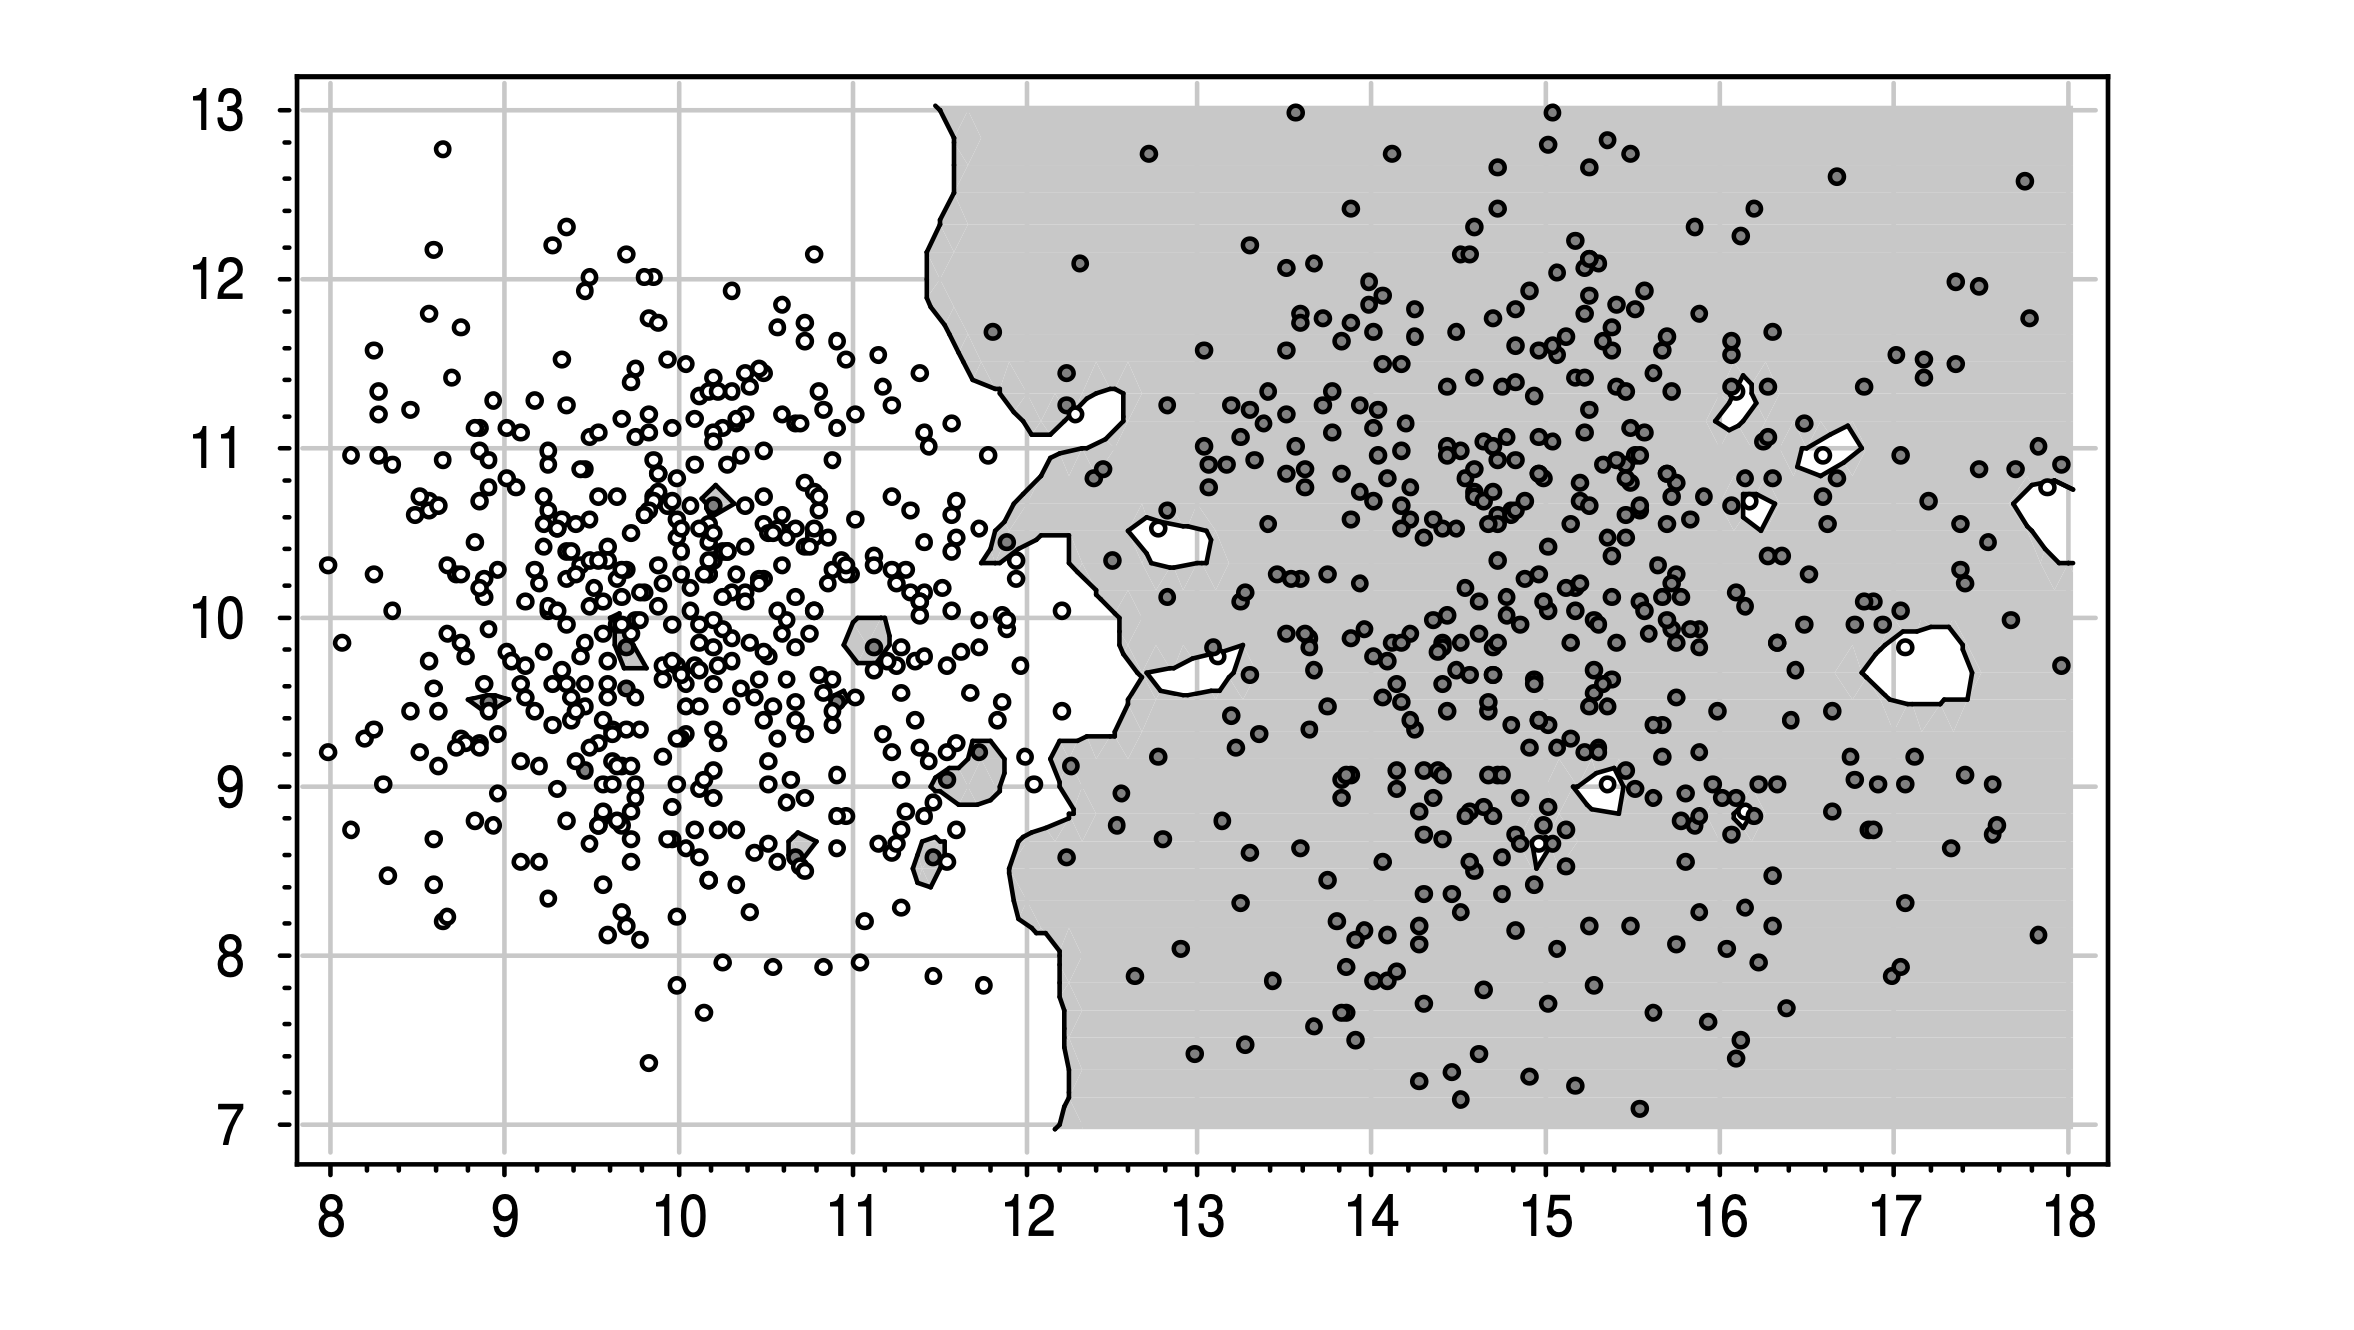
\includegraphics[width=0.5\linewidth]{experiment_1.png}

Возьмем синтетические данные по 500 объектов двух классов(оба из двухмерной гаусовской плотности), добавим 30 шумовых объектов

Последовательно удаление: \\
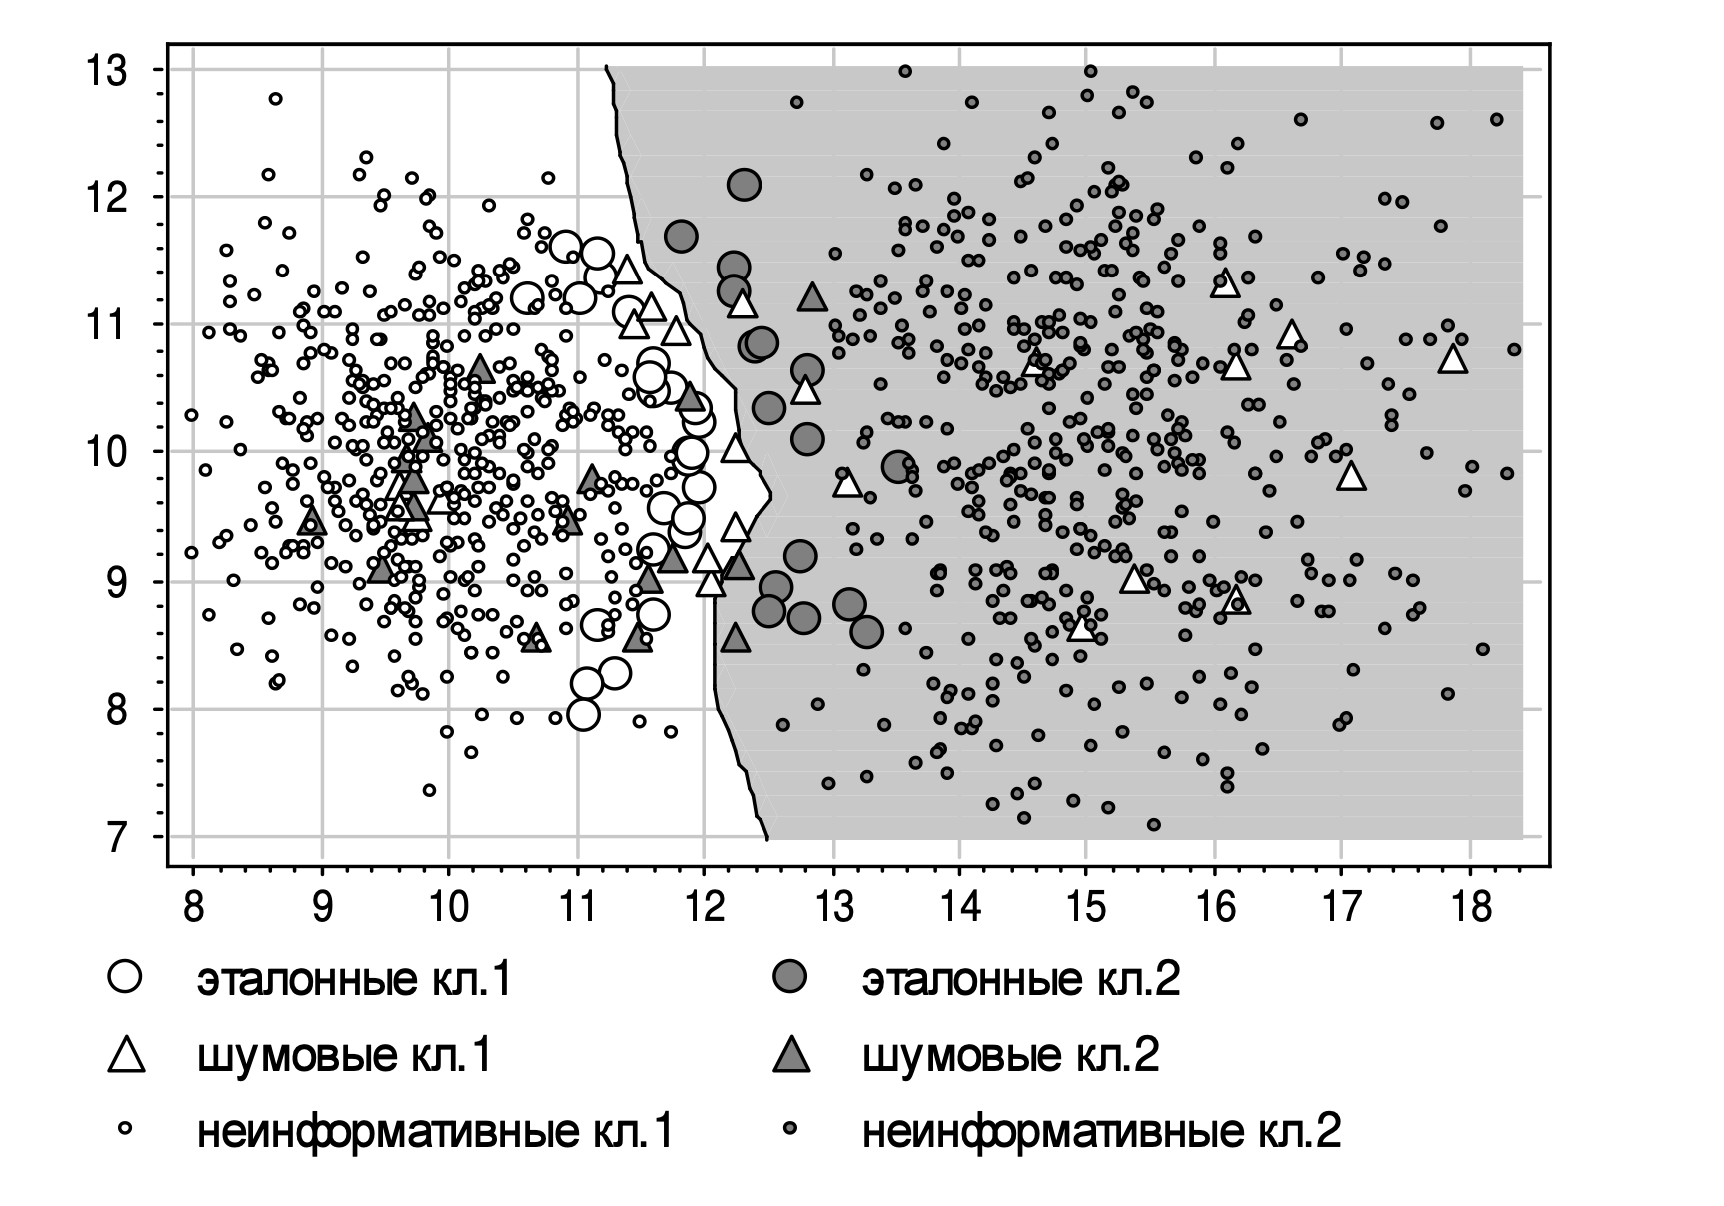
\includegraphics[width=0.5\linewidth]{experiment_2.png}

Возникают 3 типа объекта:
\begin{itemize}
    \item шумовые выбросы(30 шумов)(будут выброшены в первую очередь, тк их валидация больше всего уменьшает CCV)
    \item основная масса(окло 987)(бесполезны для классификации, так как других таких же соседей вокруг много)
    \item эталоны(стоят вдоль границы классов)
\end{itemize}

Теперь будем жадно добовлять объекты:


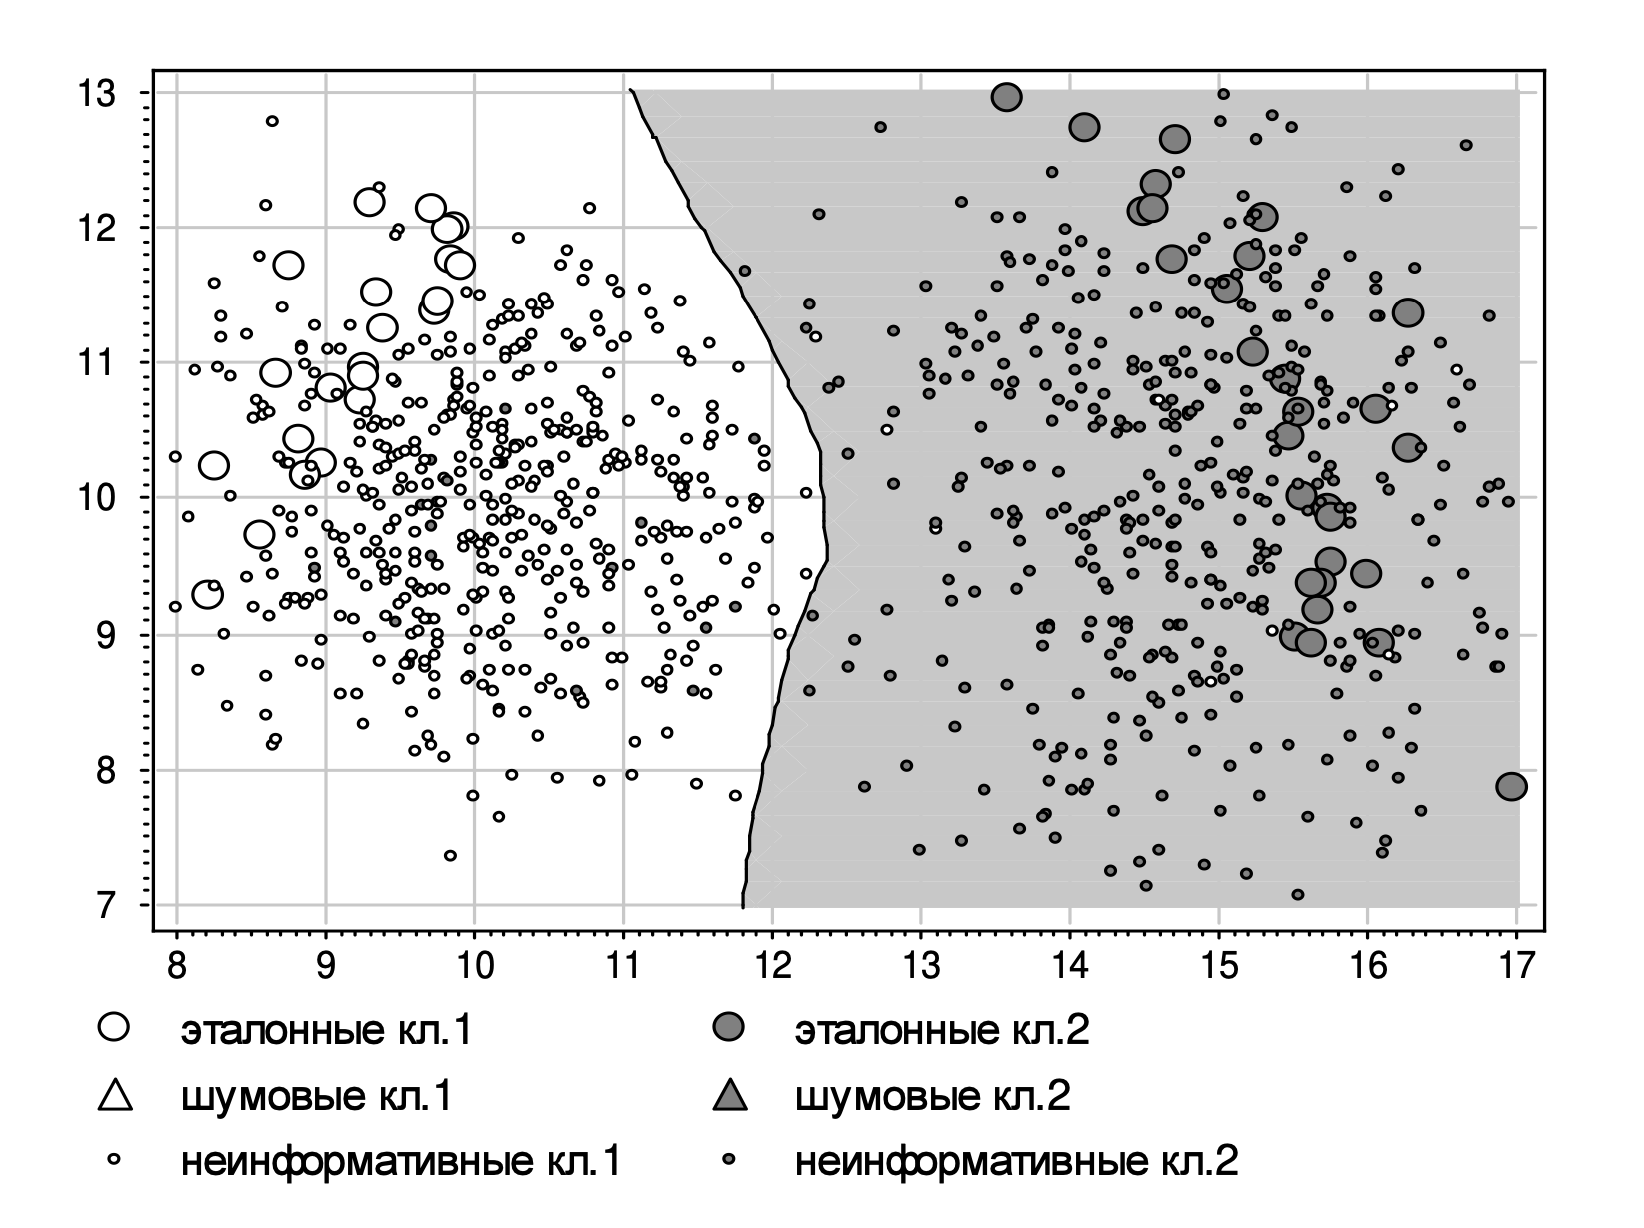
\includegraphics[width=0.5\linewidth]{experiment_3.png}

Тут же сначала возьникают эталонные точки далеко от границы класса и классификация дальше будет опираться на эти точки 



    \clearpage
    \chapter{Метод опорных векторов}
    \section{SVM-классификация}
\subsection{Постановка задачи}
\par Метод опорных векторов (Support Vector Machine, SVM) решает задачу бинарной классификации, где требуется найти оптимальную гиперплоскость, разделяющую два класса в пространстве признаков. Оптимальность понимается как максимизация ширины разделяющей полосы между классами.

\subsection{Математическая формализация}
\par Пусть дана обучающая выборка \( \{(x_i, y_i)\}_{i=1}^{\ell} \), где \( x_i \in \mathbb{R}^n \) - векторы признаков, \( y_i \in \{-1,+1\} \) - метки классов. Разделяющая гиперплоскость описывается уравнением:
\begin{equation*}
    \langle w,x \rangle - w_0 = 0,
\end{equation*}
где \( w \in \mathbb{R}^n \) - вектор весов, \( w_0 \in \mathbb{R} \) - порог.

\subsection{Условия разделимости}
\par Для корректной классификации должны выполняться условия:
\begin{equation*}
    \begin{cases}
        \langle w,x_i \rangle - w_0 \geq +1, & \text{если } y_i = +1 \\
        \langle w,x_i \rangle - w_0 \leq -1, & \text{если } y_i = -1
    \end{cases}
\end{equation*}
\par Эти условия можно объединить:
\begin{equation*}
    y_i(\langle w,x_i \rangle - w_0) \geq 1, \quad i = 1,\ldots,\ell
\end{equation*}

\subsection{Оптимизационная задача}
\par Ширина разделяющей полосы равна \( \frac{2}{\|w\|} \). Задача максимизации ширины эквивалентна задаче минимизации:
\begin{equation*}
    \frac{1}{2}\|w\|^2 \to \min_{w,w_0}
\end{equation*}
при ограничениях \( y_i(\langle w,x_i \rangle - w_0) \geq 1 \).

\subsection{Двойственная задача}
\par Применяя метод множителей Лагранжа, получаем двойственную задачу:
\begin{equation*}
    L(w,w_0,\lambda) = \frac{1}{2}\|w\|^2 - \sum_{i=1}^{\ell} \lambda_i(y_i(\langle w,x_i \rangle - w_0) - 1)
\end{equation*}
\par Условия оптимальности:
\begin{equation*}
    \begin{cases}
        w = \sum_{i=1}^{\ell} \lambda_i y_i x_i \\
        \sum_{i=1}^{\ell} \lambda_i y_i = 0
    \end{cases}
\end{equation*}

\subsection{Ядра}
\par Для нелинейной классификации используется переход в пространство признаков большей размерности через отображение \( \phi(x) \). Скалярное произведение заменяется на ядро:
\begin{equation*}
    K(x,z) = \langle \phi(x),\phi(z) \rangle
\end{equation*}
\par Популярные ядра:
\begin{itemize}
    \item Линейное: \( K(x,z) = \langle x,z \rangle \)
    \item Полиномиальное: \( K(x,z) = (\langle x,z \rangle + 1)^d \)
    \item RBF: \( K(x,z) = \exp(-\gamma\|x-z\|^2) \)
\end{itemize}

\subsection{Дискриминантная функция в ядровом пространстве}
\par После применения ядрового преобразования классификация новых точек осуществляется с помощью дискриминантной функции, которая принимает вид:
\begin{equation*}
    f(x) = \sum_{i=1}^{\ell} \lambda_i y_i K(x_i,x) - w_0
\end{equation*}
где:
\begin{itemize}
    \item \(x_i\) - опорные векторы из обучающей выборки
    \item \(\lambda_i\) - множители Лагранжа (двойственные переменные)
    \item \(y_i\) - метки классов опорных векторов
    \item \(K(x_i,x)\) - значение ядровой функции между опорным вектором и классифицируемой точкой
    \item \(w_0\) - порог, определяющий сдвиг разделяющей гиперплоскости
\end{itemize}

\par Важно отметить, что в этой формуле суммирование происходит только по опорным векторам, так как для остальных точек обучающей выборки \(\lambda_i = 0\). Это свойство обеспечивает эффективность вычислений при классификации новых точек.

\par Решающее правило для определения класса новой точки:
\begin{equation*}
    \text{class}(x) = \text{sign}(f(x)) = 
    \begin{cases}
        +1, & \text{если } f(x) > 0 \\
        -1, & \text{если } f(x) < 0
    \end{cases}
\end{equation*}

\subsection{Мягкие границы}
\par Для случая линейно неразделимой выборки вводятся переменные ослабления \( \xi_i \geq 0 \):
\begin{equation*}
    y_i(\langle w,x_i \rangle - w_0) \geq 1 - \xi_i
\end{equation*}
\par Целевая функция модифицируется:
\begin{equation*}
    \frac{1}{2}\|w\|^2 + C\sum_{i=1}^{\ell} \xi_i \to \min_{w,w_0,\xi}
\end{equation*}
где \( C > 0 \) - параметр регуляризации.

\subsection{Задача 1}
\textbf{Условие:} 
\par Дан набор точек в двумерном пространстве с метками классов:
\begin{equation*}
    \begin{array}{ll}
        x_1 = (0,0), & y_1 = -1 \\
        x_2 = (2,0), & y_2 = +1 \\
        x_3 = (0,2), & y_3 = +1 \\
        x_4 = (2,2), & y_4 = +1
    \end{array}
\end{equation*}
\par В результате обучения SVM с линейным ядром получены следующие значения двойственных переменных:
\begin{equation*}
    \lambda_1 = 0.5, \quad \lambda_2 = 0, \quad \lambda_3 = 0.5, \quad \lambda_4 = 0
\end{equation*}
\par Найдите вектор весов \(w\) и определите, является ли точка \(x_{\text{new}} = (1,1)\) опорным вектором, если известно, что она лежит точно на разделяющей гиперплоскости.

\textbf{Решение:}
\par 1. Найдем вектор весов \(w\) через опорные векторы:
\begin{equation*}
    w = \sum_{i=1}^4 \lambda_i y_i x_i
\end{equation*}

\par 2. Подставляем известные значения:
\begin{align*}
    w &= 0.5 \cdot (-1) \cdot (0,0) + 0 \cdot (+1) \cdot (2,0) + \\
    &+ 0.5 \cdot (+1) \cdot (0,2) + 0 \cdot (+1) \cdot (2,2) \\
    &= (0,0) + (0,0) + (0,0.6) + (0,0) \\
    &= (0,1)
\end{align*}

\par 3. Для точек на разделяющей гиперплоскости выполняется:
\begin{equation*}
    \langle w,x \rangle - w_0 = 0
\end{equation*}

\par 4. Подставляя координаты \(x_{\text{new}} = (1,1)\):
\begin{equation*}
    \langle (0,1),(1,1) \rangle - w_0 = 0
\end{equation*}
\begin{equation*}
    w_0 = 1
\end{equation*}

\par 5. Чтобы точка была опорным вектором, она должна лежать на границе разделяющей полосы, то есть:
\begin{equation*}
    y_{\text{new}}(\langle w,x_{\text{new}} \rangle - w_0) = \pm 1
\end{equation*}

\par 6. Проверяем это условие:
\begin{equation*}
    \langle (0,1),(1,1) \rangle - 1 = 0
\end{equation*}
Получаем 0, что не равно $\pm1$.

\textbf{Ответ:} \(w = (0,1)\). Точка \(x_{\text{new}}\) не является опорным вектором.

\subsection{Задача 2}
\textbf{Условие:} 
\par Дано множество точек в двумерном пространстве:
\begin{equation*}
    \begin{array}{ll}
        x_1 = (1,1), & y_1 = +1 \\
        x_2 = (2,2), & y_2 = +1 \\
        x_3 = (0,0), & y_3 = -1 \\
        x_4 = (-1,1), & y_4 = -1
    \end{array}
\end{equation*}
\par После обучения SVM получена разделяющая гиперплоскость \(2/3 \cdot x_{i1} + 1/3 \cdot x_{i2} - 1 = 0\). Определите, какие из точек являются опорными векторами.

\textbf{Решение:}
\par Опорными векторами являются точки, лежащие на границе разделяющей полосы. Для их определения нужно:

\par 1. Запишем вектор весов из уравнения гиперплоскости:
\begin{equation*}
    w = (2/3,1/3) \quad w_0 = 1
\end{equation*}

\par 2. Вычислим отступ для каждой точки по формуле:
\begin{equation*}
    M(x) = y(\langle w,x \rangle - w_0) = y(2x_{i1} + x_{i2} - 3)
\end{equation*}

\par 3. Проверяем каждую точку:
\begin{align*}
    M(x_1) &= (+1)(2/3 \cdot 1 + 1/3 \cdot 1 - 1) = 0 \\
    M(x_2) &= (+1)(2/3 \cdot 2 + 1/3 \cdot 2 - 1) = 1 \\
    M(x_3) &= (-1)(2/3 \cdot 0 + 1/3 \cdot 0 - 1) = 1 \\
    M(x_4) &= (-1)(2/3 \cdot (-1) + 1/3 \cdot 1 - 1) = 4/3
\end{align*}

\par 4. Опорными векторами являются точки с отступом, равным единице, а также точки, лежащие на разделяющей гиперплоскости (отступ равен нулю).

\textbf{Ответ:} Точки \(x_2\) и \(x_3\) являются опорными векторами.

\subsection{Задача 3}
\textbf{Условие:} 
\par При обучении SVM с полиномиальным ядром второй степени \(K(x,z) = (\langle x,z \rangle + 1)^2\) получены следующие опорные векторы:
\begin{equation*}
    \begin{array}{ll}
        x_1 = (2,0), & \lambda_1 = 0.2, \quad y_1 = +1 \\
        x_2 = (0,1), & \lambda_2 = 0.3, \quad y_2 = -1 \\
        x_3 = (1,1), & \lambda_3 = 0.1, \quad y_3 = +1
    \end{array}
\end{equation*}
\par К какому классу будет отнесена точка \(x_{\text{new}} = (1,0)\), если \(w_0 = 0.5\)?

\textbf{Решение:}
\par Для определения класса точки нужно найти знак дискриминантной функции:
\begin{equation*}
    f(x) = \sum_{i=1}^3 \lambda_i y_i K(x_i,x) - w_0
\end{equation*}

\par Вычислим значения ядра для \(x_{\text{new}}\) и каждого опорного вектора:
\begin{align*}
    K(x_1,x_{\text{new}}) &= (2 \cdot 1 + 0 \cdot 0 + 1)^2 = 9 \\
    K(x_2,x_{\text{new}}) &= (0 \cdot 1 + 1 \cdot 0 + 1)^2 = 1 \\
    K(x_3,x_{\text{new}}) &= (1 \cdot 1 + 1 \cdot 0 + 1)^2 = 4
\end{align*}

\par Подставляем в дискриминантную функцию:
\begin{align*}
    f(x_{\text{new}}) &= 0.2 \cdot (+1) \cdot 9 + 0.3 \cdot (-1) \cdot 1 + 0.1 \cdot (+1) \cdot 4 - 0.5 \\
    &= 1.8 - 0.3 + 0.4 - 0.5 = 1.4
\end{align*}

\par Так как \(f(x_{\text{new}}) > 0\), точка относится к классу +1.

\textbf{Ответ:} Точка \(x_{\text{new}}\) будет отнесена к классу +1.

\section{SVM-регрессия}
\subsection{Постановка задачи}
\par В задаче регрессии требуется найти функцию \( f(x) = w^T \phi(x) + b \), которая аппроксимирует целевые значения \( y \) на основе входных данных \( x \), минимизируя ошибки предсказания.
\par В SVM-регрессии вводится допустимая область погрешностей — \(\epsilon\)-окрестность. Это означает, что отклонения \( |f(x_i) - y_i| \) в пределах \(\epsilon\) считаются несущественными, и модель игнорирует их. Цель — минимизировать сложность модели, связанную с \(\|w\|\), штрафуя при этом за отклонения, выходящие за пределы \(\epsilon\).

\subsection{Прямая задача}
\par\textbf{Функция потерь.}  
Для задачи SVM-регрессии используется \(\epsilon\)-чувствительная функция потерь:
\begin{equation*}
    L_\epsilon(f(x), y) = 
    \begin{cases} 
        0, & \text{если } |f(x) - y| \leq \epsilon, \\ 
        |f(x) - y| - \epsilon, & \text{иначе.}
    \end{cases}
\end{equation*}
\noindent\textbf{Прямая постановка задачи:}
\begin{equation*}
    \min_{w, b} \frac{1}{2} \|w\|^2 + C \sum_{i=1}^n L_\epsilon(f(x_i), y_i),
\end{equation*}
где:
\begin{itemize}
    \item \(\|w\|^2\) — регуляризационный член, минимизирующий сложность модели,
    \item \(C\) — коэффициент, регулирующий баланс между штрафами за ошибки и сложностью модели,
    \item \(L_\epsilon(f(x_i), y_i)\) — штраф за выход за пределы \(\epsilon\)-окрестности.
\end{itemize}

\subsection{Преобразование задачи}
\par Для учёта отклонений выше \(\epsilon\) вводятся штрафные переменные \(\xi_i\) и \(\xi_i^*\):  
\begin{itemize}
    \item \(\xi_i\) — превышение сверху (\(y_i > f(x_i) + \epsilon\)),
    \item \(\xi_i^*\) — превышение снизу (\(y_i < f(x_i) - \epsilon\)).
\end{itemize}
\par Задача минимизации принимает вид:
\begin{equation*}
    \min_{w, b, \xi, \xi^*} \frac{1}{2} \|w\|^2 + C \sum_{i=1}^n (\xi_i + \xi_i^*),
\end{equation*}
при ограничениях:
\begin{equation*}
\begin{aligned}
    y_i - (w^T \phi(x_i) + b) \leq \epsilon + \xi_i, \\
    (w^T \phi(x_i) + b) - y_i \leq \epsilon + \xi_i^*, \\
    \xi_i, \xi_i^* \geq 0.
\end{aligned}
\end{equation*}

\subsection{Метод Лагранжа}
\par Для решения задачи вводится лагранжиан, который включает:
\begin{itemize}
    \item Целевую функцию,
    \item Ограничения через множители Лагранжа (\(\alpha, \alpha^*, \eta, \eta^*\)).
\end{itemize}
\par Лагранжиан записывается как:
\begin{equation*}
\begin{aligned}
    L(w, b, \xi, \xi^*, \alpha, \alpha^*, \eta, \eta^*) &= \frac{1}{2} \|w\|^2 + C \sum_{i=1}^n (\xi_i + \xi_i^*) - \\
    &\quad - \sum_{i=1}^n \alpha_i \big[ \epsilon + \xi_i - y_i + w^T \phi(x_i) + b \big] - \\
    &\quad - \sum_{i=1}^n \alpha_i^* \big[ \epsilon + \xi_i^* + y_i - w^T \phi(x_i) - b \big] - \\
    &\quad - \sum_{i=1}^n (\eta_i \xi_i + \eta_i^* \xi_i^*).
\end{aligned}
\end{equation*}
\par Для нахождения двойственной задачи необходимо минимизировать \(L\) по \(w\), \(b\), \(\xi\), \(\xi^*\) и максимизировать по множителям Лагранжа.

\subsection{Условия оптимальности}
\begin{enumerate}
    \item Производная по \(w\):
    \begin{equation*}
        \frac{\partial L}{\partial w} = w - \sum_{i=1}^n (\alpha_i - \alpha_i^*) \phi(x_i) = 0 \implies 
        w = \sum_{i=1}^n (\alpha_i - \alpha_i^*) \phi(x_i).
    \end{equation*}
    \item Производная по \(b\):
    \begin{equation*}
        \frac{\partial L}{\partial b} = \sum_{i=1}^n (\alpha_i - \alpha_i^*) = 0.
    \end{equation*}
    \item Производные по \(\xi_i\) и \(\xi_i^*\):
    \begin{equation*}
        \alpha_i + \eta_i = C, \quad \alpha_i^* + \eta_i^* = C, \quad 0 \leq \alpha_i, \alpha_i^* \leq C.
    \end{equation*}
\end{enumerate}

\subsection{Двойственная задача}
\par Подставляя условия оптимальности в лагранжиан, исключаем \(w\), \(b\), \(\xi_i\), \(\xi_i^*\). Получаем двойственную задачу:
\begin{equation*}
    \max_{\alpha, \alpha^*} -\frac{1}{2} \sum_{i,j=1}^n (\alpha_i - \alpha_i^*)(\alpha_j - \alpha_j^*) K(x_i, x_j) 
    - \epsilon \sum_{i=1}^n (\alpha_i + \alpha_i^*) + \sum_{i=1}^n y_i (\alpha_i - \alpha_i^*),
\end{equation*}
где \(K(x_i, x_j) = \phi(x_i)^T \phi(x_j)\) — ядровая функция.
\par Ограничения:
\begin{equation*}
    \sum_{i=1}^n (\alpha_i - \alpha_i^*) = 0, \quad 0 \leq \alpha_i, \alpha_i^* \leq C.
\end{equation*}
\par Для решения двойственной задачи используется метод квадратичного программирования.

\subsection{Построение финальной модели}
\par После решения двойственной задачи оптимальные \(\alpha_i\) и \(\alpha_i^*\) определяют параметры модели:
\begin{equation*}
    f(x) = \sum_{i=1}^n (\alpha_i - \alpha_i^*) K(x_i, x) + b.
\end{equation*}
\par Смещение \(b\) вычисляется через опорные векторы — точки, где выполняется одно из условий:
\begin{equation*}
    y_i - (w^T \phi(x_i) + b) = \epsilon, \quad \text{или} \quad y_i - (w^T \phi(x_i) + b) = -\epsilon.
\end{equation*}
\par Опорные векторы (\(\alpha_i > 0\) или \(\alpha_i^* > 0\)) определяют форму модели.

\subsection{Выбор ядра}
\par Выбор ядра играет ключевую роль в качестве работы модели SVM-регрессии. Различные ядра по-разному преобразуют входные данные, что может существенно повлиять на точность предсказаний и обобщающую способность модели.
\par Выбор ядра зависит от особенностей данных, структуры зависимости и доступных вычислительных ресурсов. Экспериментальная проверка нескольких типов ядер и последующая оценка метрик качества модели — это ключевой этап в процессе выбора оптимального ядра.
\par На рисунке ниже представлена SVM-регрессия с тремя типами ядер: RBF, линейным и полиномиальным. 
\begin{figure}[ht!]
    \includegraphics[width = 0.8\textwidth]{chapters/svm/images/svm_regression_cmp_models.png}
    \centering
    \caption{Сравнение SVM-регрессия с разными типами ядер}
    \label{fig:kernel_comparison}
\end{figure}

\subsection{Задача 1}
\textbf{Условие}:
\par Рассмотрим следующий набор точек, лежащих на границе \(\epsilon\) - окрестности для SVM-регрессии с линейным ядром:
\begin{equation*}
    \{(1, 2), (2, 3), (3, 5), (4, 6)\}
\end{equation*}
\par Постройте регрессионную модель и найдите смещение \(b\), если \(w = 2\), \(\epsilon = 1\).
\par \noindent \textbf{Решение:}
\par Для нахождения смещения \(b\) необходимо использовать точки, которые лежат на границах \(\epsilon\)-окрестности. Мы знаем, что для таких точек выполняется равенство:
\begin{equation*}
    y_i - (w x_i + b) = \epsilon \quad \text{или} \quad y_i - (w x_i + b) = -\epsilon
\end{equation*}
\par Найдем для каждой точки \(b\), подставив их координаты в эти уравнения:
\begin{itemize}
\item Для точки \((1, 2)\):
\begin{equation*}
    2 - (2 \cdot 1 + b) = 1 \quad \Rightarrow \quad 2 - (2 + b) = 1 \quad \Rightarrow \quad -b = 1 \quad \Rightarrow \quad b = -1
\end{equation*}
\item Для точки \((2, 3)\):
\begin{equation*}
    3 - (2 \cdot 2 + b) = 1 \quad \Rightarrow \quad 3 - (4 + b) = 1 \quad \Rightarrow \quad -b = 2 \quad \Rightarrow \quad b = -2
\end{equation*}
\item Для точки \((3, 5)\):
\begin{equation*}
    5 - (2 \cdot 3 + b) = 1 \quad \Rightarrow \quad 5 - (6 + b) = 1 \quad \Rightarrow \quad -b = 2 \quad \Rightarrow \quad b = -2
\end{equation*}
\item Для точки \((4, 6)\):
\begin{equation*}
    6 - (2 \cdot 4 + b) = 1 \quad \Rightarrow \quad 6 - (8 + b) = 1 \quad \Rightarrow \quad -b = 3 \quad \Rightarrow \quad b = -3
\end{equation*}
\end{itemize}
\par Для вычисления окончательного значения смещения \(b\), усредняем найденные значения:
\begin{equation*}
    b_{\text{avg}} = \frac{-1 + (-2) + (-2) + (-3)}{4} = \frac{-8}{4} = -2
\end{equation*}
\par Таким образом, смещение \(b = -2\).
\par Регрессионная модель для SVM с линейным ядром имеет следующий вид:
\begin{equation*}
    f(x) = w x + b
\end{equation*}
\par Подставляем данное в условии значения \(w = 2\) и найденное значение \(b = -2\):
\begin{equation*}
    f(x) = 2x - 2
\end{equation*}
\par Это и есть наша линейная регрессионная модель.
\par \noindent \textbf{Ответ:} \(f(x) = 2x - 2\).

\subsection{Задача 2}
\textbf{Условие:}
\par У нас есть два набора данных для задачи регрессии:
\begin{itemize}
    \item Набор 1: \( \{(1, 2), (2, 3), (3, 4), (4, 5)\} \)    
    \item Набор 2: \( \{(1, 1), (2, 4), (3, 9), (4, 16)\} \)  
\end{itemize}
\par Предположим, что мы используем SVM-регрессию с различными типами ядер (линейное, полиномиальное, RBF). Определите, какое ядро будет оптимальным для каждого набора данных.
\par \noindent \textbf{Решение:}
\begin{itemize}
    \item Набор 1: данные имеют линейную зависимость, следовательно, линейное ядро будет лучшим выбором.

    \item Набор 2: данные имеют квадратичную зависимость, следовательно, оптимально будет использовать полиномиальное ядро второй степени.
\end{itemize}
\par \noindent \textbf{Ответ:} для первого набора данных оптимальным ядром будет линейное, для второго набора данных - полиномиальное второй степени.

\subsection{Задача 3}
\textbf{Условие:}
\par Дан набор данных для SVM-регрессии с линейным ядром: 
\begin{equation*}
    \{(1, 2), (2, 2.8), (3, 5.2), (4, 8)\}.
\end{equation*}
\par Параметры модели: \(w = 1.5\), \(b = 0.5\), \(\epsilon = 0.5\). 
\begin{enumerate}
    \item Определите, какие из точек набора данных находятся вне \(\epsilon\)-окрестности (требуют штрафных переменных \(\xi\) или \(\xi^*\)).
    \item Вычислите значения штрафных переменных для этих точек.
\end{enumerate}
\par \noindent \textbf{Решение:}
\begin{enumerate}
\item Определение границ \(\epsilon\)-окрестности:
   Уравнение модели SVM-регрессии с линейным ядром: 
   \begin{equation*}
    f(x) = wx + b.
   \end{equation*}
   Подсталяем данные в условии значения:
   \begin{equation*}
    f(x) = 1.5x + 0.5.
   \end{equation*}
   Границы \(\epsilon\)-окрестности:
   \begin{equation*}
    f(x) - \epsilon \leq y \leq f(x) + \epsilon.
   \end{equation*}
\item Проверка точек:
\begin{itemize}
    \item Для точки \((1, 2)\): 
    \begin{equation*}
        f(1) = 1.5 \cdot 1 + 0.5 = 2.0, \quad 2 - 0.5 \leq 2 \leq 2 + 0.5 \quad (\text{в окрестности}).
    \end{equation*}
    \item Для точки \((2, 2.8)\): 
    \begin{equation*}
        f(2) = 1.5 \cdot 2 + 0.5 = 3.5, \quad 3.5 - 0.5 \not\leq 2.8 \leq 3.5 + 0.5 \quad (\text{вне окрестности}).
    \end{equation*}
    \item Для точки \((3, 5.2)\): 
    \begin{equation*}
        f(3) = 1.5 \cdot 3 + 0.5 = 5.0, \quad 5.0 - 0.5 \leq 5.2 \leq 5.0 + 0.5 \quad (\text{в окрестности}).
    \end{equation*}
    \item Для точки \((4, 8)\): 
    \begin{equation*}
        f(4) = 1.5 \cdot 4 + 0.5 = 6.5, \quad 6.5 - 0.5 \leq 8.0 \not\leq 6.5 + 0.5 \quad (\text{вне окрестности}).
    \end{equation*}
\end{itemize}
\item Штрафные переменные:
\begin{itemize}
    \item Для точки \((2, 2.8)\):
    \begin{equation*}
        \xi_i = f(2) - y - \epsilon = 3.5 - 2.8 - 0.5 = 0.2.
    \end{equation*}
    \item Для точки \((4, 8)\):
    \begin{equation*}
        \xi_i^* = y - f(4) - \epsilon = 8 - 6.5 - 0.5 = 1.0.
    \end{equation*}
\end{itemize}
Таким образом, штрафные переменные:
\begin{equation*}
    \xi_2^* = 0.2, \quad \xi_4 = 1.0.
\end{equation*}
\end{enumerate}
\par \noindent \textbf{Ответ:} \(\xi_2^* = 0.2, \quad \xi_4 = 1.0.\)


\setcounter{secnumdepth}{0}

\section{1-norm SVM (LASSO SVM)}
\subsection*{Аппроксимация эмпирического риска с \(L_1\)-регуляризацией}
\begin{align*}
    \sum_{i=1}^{\ell} \left(1 - M_i(w, w_0)\right)_+ + \mu \sum_{j=1}^{n} |w_j| & \rightarrow \min_{w, w_0}
\end{align*}

\subsection*{Плюс: отбор признаков с параметром селективности \(\mu\)}
\begin{itemize}
    \item чем больше \(\mu\), тем меньше признаков останется
\end{itemize}

\subsection*{Минус: слишком агрессивный отбор признаков}
\begin{itemize}
    \item по мере увеличения \(\mu\) признак может быть отброшен, хотя $y$ существенно зависит от него (даже когда ещё не все шумовые признаки отброшены)
\end{itemize}

\vspace{10pt}

\section{Сравнение L2 и L1 регуляризации}

Зависимость весов \(w_j\) от коэффициента \(\frac{1}{\mu}\):

\begin{itemize}
    \item \(L_1\) регуляризатор: \(\mu \sum_{j} |w_j|\)
\end{itemize}

\begin{figure}[ht]
    \centering
    \includegraphics[width=0.6 \linewidth]{chapters/svm/images/L_1.png}
    \label{fig:image_1}    
\end{figure}

\begin{itemize}
    \item \(L_2\) регуляризатор: \(\mu \sum_{j} w_j^2\)
\end{itemize}

\begin{figure}[ht]
    \centering
    \includegraphics[width=0.6 \linewidth]{chapters/svm/images/L_2.png}
    \label{fig:image_2}    
\end{figure}

\section{Doubly Regularized SVM (Elastic Net SVM)}

\begin{align*}
    C \sum_{i=1}^{\ell} \left(1 - M_i(w, w_0)\right)_+ + \mu \sum_{j=1}^{n} |w_j| + \frac{1}{2} \sum_{j=1}^{n} w_j^2 & \rightarrow \min_{w, w_0}
\end{align*}

\subsection*{Плюсы:}
\begin{itemize}
    \item Параметр селективности \(\mu\) управляет отбором признаков: чем больше \(\mu\), тем меньше признаков останется
    \item Есть эффект группировки (grouping effect): значимые зависимые признаки отбираются вместе
\end{itemize}

\subsection*{Минусы:}
\begin{itemize}
    \item Шумовые признаки также группируются и могут вместе оставаться в модели
    \item Приходится подбирать два параметра регуляризации \(\mu, \tau\) (есть специальные методы, например, regularization path)
\end{itemize}

\subsection{Elastic Net Analysis}

Elastic Net менее жёстко отбирает признаки.

\begin{figure}[ht]
    \centering
    \includegraphics[width=0.8\linewidth]{chapters/svm/images/Elastic_Net.png}
    \caption{Зависимости весов \(w_j\) от коэффициента \(\log \frac{1}{\mu}\)}
    \label{fig:elastic_net}
\end{figure}

\section{Support Features Machine (SFM)}

\begin{align*}
    C \sum_{i=1}^{\ell} \left(1 - M_i(w, w_0)\right)_+ + \sum_{j=1}^{n} R_{\mu}(w_{j}) & \rightarrow \min_{w, w_0}
\end{align*}

\begin{align*}
R_{\mu}(w_j)=
    \begin{cases}
        2\mu |w_j|, & |w_j| \leq \mu\\
        \mu^2 + w_j^2, & |w_j| \geq \mu \\
    \end{cases}
\end{align*}

\subsection*{Плюсы}
\begin{itemize}
    \item Только один параметр регуляризации \(\mu\)
    \item Отбор признаков с параметром селективности \(\mu\)
    \item Эффект группировки: значимые зависимые признаки ($|w_j|$ > \(\mu\)) входят в решение совместно (как в $Elastic$ $Net$)
    \item Шумовые признаки ($|w_j|$ < \(\mu\)) не группируются и подавляются независимо друг от друга (как в $LASSO$)
\end{itemize}

\section{Relevance Features Machine (RFM)}

\begin{align*}
    C \sum_{i=1}^{\ell} \left(1 - M_i(w, w_0)\right)_+ + \sum_{j=1}^{n} \ln(w_j^2 + \frac{1}{\mu}) & \rightarrow \min_{w, w_0}
\end{align*}

\begin{align*}
    R(w) = \ln(w^2 + \frac{1}{\mu}), \quad \mu = 0.1, 1, 100
\end{align*}

\subsection*{Плюсы}
\begin{itemize}
    \item Только один параметр регуляризации \(\mu\)
    \item Отбор признаков с параметром селективности \(\mu\)
    \item Есть эффект группировки
    \item Лучше отбирает набор значимых признаков, когда они только совместно обеспечивают хорошее решение
\end{itemize}

\section{Задачи}

\subsection{Задача 1}

Качественно объяснить, почему $L_1$-регуляризатор приводит к отбору признаков

\subsection{Ответ:}

Аппроксимация эмпирического риска с \(L_1\)-регуляризацией:
\begin{align*}
    \sum_{i=1}^{\ell} \left(1 - M_i(w, w_0)\right)_+ + \mu \sum_{j=1}^{n} |w_j| & \rightarrow \min_{w, w_0}
\end{align*}

\textcolor{red}{Почему \(L_1\)-регуляризатор приводит к отбору признаков?}

Замена переменных: 
\[
u_j = \frac{1}{2} (|w_j| + w_j), \quad v_j = \frac{1}{2} (|w_j| - w_j).
\]
Тогда 
\[
w_j = u_j - v_j \quad |w_j| = u_j + v_j.
\]

\begin{align*}
    \sum_{i=1}^{\ell} \left(1 - M_i(u - v, w_0)\right)_+ + \mu \sum_{j=1}^{n} (u_j + v_j) & \rightarrow \min_{u, v}, \\
    u_j \geq 0, \quad v_j \geq 0, \quad j = 1, \ldots, n.
\end{align*}

чем больше \(\mu\), тем больше индексов \(j\) таких, что \(u_j = v_j = 0\), но тогда \(w_j = 0\), значит, \textcolor{red}{признак не учитывается.}

\subsection{Задача 2}

Привести пример нежелательного эффекта в процессе обучения, с которым поможет справиться регуляризация 
 
\subsection{Ответ:}

Регуляризация помогает в случае линейной зависимости (мультиколлинеарности) признаков:\\
Пусть построен классификатор: $a(x, w) = sign\langle w, x \rangle$ \\
Мультиколлинеарность: $\exists$  $u \in \mathbb{R}^{n}$: $\forall x \in X$ $\langle u, x \rangle = 0$ \\
Неединственность решения и рост нормы вектора весов: $\forall \gamma \in \mathbb{R}$ $a(x, w) = sign\langle w, x \rangle = sign \langle w + \gamma u, x \rangle$ \\
\\
Проявления переобучения:
\begin{itemize}
    \item слишком большие веса $|w_j|$ разных знаков
    \item неустойчивость дискриминантной функции $\langle w, x \rangle$
    \item $Q(X^{\ell}) \ll Q(X^{k})$
\end{itemize}
Способ уменьшить переобучение:\\
регуляризация $||w|| \rightarrow min$ (сокращение весов, $weight$ $decay$)

\subsection{Задача 3}

Дана задача оптимизации:
\begin{align*}
    \frac{1}{2}(wx - b)^2 + \lambda|w| & \rightarrow \min_{w},
\end{align*}
где $x,$ $b$ $\in \mathbb{R};$ $\lambda \geq 0$\\
При каких $\lambda$ данная задачи имеет решение $w_0 \neq 0?$
 
\subsection{Ответ:}

Находим правую и левую односторонние производные в нуле и рассматриваем, когда они больше и меньше 0 соответственно:

\begin{align*}
    \begin{cases}
        -xb + \lambda > 0\\
        -xb - \lambda < 0\\
        \lambda \geq 0\\
    \end{cases} \Leftrightarrow \lambda > |xb|
\end{align*}

Это условие на $\lambda,$ при котором задача имеет решение $w_0 = 0,$ поэтому нам подходит $\lambda \in [0;$ $|xb|)$.


\section{Ядерные функции машины опорных векторов}
При наличии нелинейной связи между признаками и откликом качество линейных классификаторов, как показано на рисунке ниже,
часто может оказаться неудовлетворительным.
\begin{align*}
    \centering
    \includegraphics[width=0.6 \linewidth]{chapters/svm/images/svm_kernels.png}
    \label{fig:image}
\end{align*}
Для учета нелинейности обычно расширяют пространство переменных,
включая различные функциональные преобразования исходных предикторов (полиномы, экспоненты и проч.).
Машину опорных векторов SVM (Support Vector Machine) можно рассматривать как нелинейное обобщение линейного классификатора, полученного при
решении двойственной задачи (прямая задача является задачей бинарной классификации):
$$
\left\{\begin{array}{l}
w=\sum_{i=1}^{\ell} \lambda_i y_i x_i ; \\
w_0=\left\langle w, x_i\right\rangle-y_i, \quad \text { для любого } i: \lambda_i>0, M_i=1 .
\end{array}\right.
$$

Линейный классификатор с признаками $f_i(x)=\left\langle x, x_i\right\rangle$ :
$$
a(x)=\operatorname{sign}\left(\sum_{i=1}^{\ell} \lambda_i y_i\left\langle x, x_i\right\rangle-w_0\right) .
$$

Введя здесь новую нелинейную функцию $K\left(x, x^{\prime}\right)$, вместо $\left\langle x, x^{\prime}\right\rangle$,
можно строить модели с разделяющих поверхностями самой различной формы.

Дадим формальное определение:\newline
\textbf{Oпределение}:\newline
Функция $K: X \times X \rightarrow \mathbb{R}-$ ядро, если $K\left(x, x^{\prime}\right)=\left\langle\psi(x), \psi\left(x^{\prime}\right)\right\rangle$
при некотором $\psi: X \rightarrow H$, где $H-$ гильбертово пространство. \newline
В качестве таких функций чаще всего используют следующие:
\begin{itemize}
\item линейное ядро: $K(x, x^{\prime})=\langle x, x^{\prime} \rangle$, что соответствует классификатору на опорных векторах в исходном пространстве (см. рис. 6.3);
\item полиномиальное ядро со степенью $p: K(x, x^{\prime})=(1+\langle x, x^{\prime} \rangle)^p$;
\item гауссово ядро с радиальной базовой функцией (RBF): $K(x, x^{\prime})=\exp(\gamma\langle x - x^{\prime} \rangle^2)$;
\item сигмодиное ядро: $K(x, x^{\prime})=\tanh(\gamma\langle x, x^{\prime}\rangle+\beta_0)$.
\end{itemize}

Для того, чтобы определять является ли функция ядром, существует\newline
\textbf{Теорема Мерсера}:\newline
Функция двух переменных $K\left(x, x^{\prime}\right)$ является ядром тогда и только тогда, когда она
\begin{itemize}
\item симметрична, то есть $K\left(x, x^{\prime}\right)=K\left(x^{\prime}, x\right)$;
\item неотрицательно определена, то есть $\int_X \int_X K\left(x, x^{\prime}\right) g(x) g\left(x^{\prime}\right) d x d x^{\prime} \geq 0$ для любой функции $g: X \rightarrow \mathbb{R}$;
\end{itemize}

Нужно отметить, что на практике проверка неотрицательной определенности функции $K\left(x, x^{\prime}\right)$ часто является нелегкой задачей.
Вместо этого обычно используют какие-то конструктивные методы синтеза ядер, например достаточно очевидное утверждение: $K\left(x, x^{\prime}\right)=\alpha_1 K_1\left(x, x^{\prime}\right)+\alpha_2 K_2\left(x, x^{\prime}\right)$ при $\alpha_1, \alpha_2>0-$ ядро.

\subsection{Задача 1}
Найти пространство $H$ и преобразование $\psi: X \rightarrow H$, при которых
$K(x, x^{\prime}) = \langle \psi(x),\psi(x^{\prime}) \rangle $, где $X = \mathbb{R}^n,~
K(x, x^{\prime}) = \langle x, x^{\prime} \rangle^2,~ x = (x_1, x_2, \cdots x_n),~ x^{\prime} = (x_1^{\prime}, x_2^{\prime}, \cdots x_n^{\prime})$
\subsection{Решение}
\begin{align*}
K(x, x^{\prime}) = \langle x, x^{\prime} \rangle^2 = \langle (x_1, x_2, \cdots x_n), (x_1^{\prime}, x_2^{\prime}, \cdots x_n^{\prime}) \rangle^2 = (x_1x_1^{\prime} + \cdots + x_nx_n^{\prime})^2  \\
  = x_1^2x_1^{\prime}^2 + \cdots + \cdots x_n^2x_n^{\prime}^2 + 2x_1x_1^{\prime}x_2x_2^{\prime} + \cdots 2x_1x_1^{\prime}x_{n}x_n^{\prime} + \cdots + 2x_{n-1}x_{n-1}^{\prime}x_{n}x_{n}^{\prime}  = \\
  = \langle(x_1^2, x_2^2, \cdots x_n^2, \sqrt{2}x_1x_2, \cdots \sqrt{2}x_{n-1}x_n),(x_1^{\prime}^2, x_2^{\prime}^2, \cdots x_n^{\prime}^2, \sqrt{2}x_1^{\prime}x_2^{\prime},\cdots \sqrt{2}x_{n-1}^{\prime}x_{n}^{\prime})\rangle
\end{align*}
Подсчетом слагаемых можно убедиться, что $ dimH = \frac{1}{2}n(n-1) $, а $\psi:(x_1, x_2, \cdots x_n) \mapsto(x_1^2, x_2^2, \cdots x_n^2, \sqrt{2}x_1x_2, \cdots \sqrt{2}x_{n-1}x_n)$

\subsection{Задача 2}
Доказать, что $\forall \psi: X \rightarrow \mathbb{R}$ произведение $K\left(x, x^{\prime}\right)=\psi(x) \psi\left(x^{\prime}\right)-$ ядро.
\subsection{Решение}

Действительно, произведение $\psi(x) \psi(x^{\prime})$ есть скалярное произведение в одномерном пространстве $\mathbb{R}$, а в силу свойств скалярного произведения
(положительная определенность и симметричность) по теореме Мерсера получаем, что $K(x, x^{\prime})$ ядро.

\subsection{Задача 3}
Доказать, что $K(x, x^{\prime})=\exp(\langle x - x^{\prime} \rangle^2)$ ядро (гауссово ядро с радиальной базовой функцией).
\subsection{Решение}

Для доказательство нужно воспользоваться утверждением: композиция произвольного ядра $K_0$ и произвольной функции
$f: \mathbb{R} \rightarrow \mathbb{R}$, представимой в виде сходящегося степенного ряда с неотрицательными коэффициентами
$K\left(x, x^{\prime}\right)=f\left(K_0\left(x, x^{\prime}\right)\right)$, является ядром.
$K_0(x, x^{\prime}) = \langle x - x^{\prime} \rangle^2$ является ядром по свойствам скалярного произведения. Как известно,
экспонента представима в виде степенного ряда с положительными коэффициентами, поэтому выполнены все условия утверждения, что
доказывает, что $K(x, x^{\prime})$ ядро.


\section{Relevance Vector Machine(RVM)}

\subsection{Идея метода релевантных векторов}

Берем за основу структуру решения как в SVM:\\
\begin{align*}
   \sum_{i=1}^{\ell} \lambda_i y_i x_i
\end{align*}

(опорным векторам $x_i$ соответствуют $\lambda_i \neq 0$) \\
\textbf{Проблема:} Какие из коэффициентов $\lambda_i$ лучше обнулить? \\
Делаем так, что регуляризатор зависит не от w, а от $\lambda_i$. \\
\begin{align*}
       \rho (\lambda) = \frac{1}{(2\pi)^{l/2} \sqrt{\alpha_1...\alpha_l}} exp(-\sum_{i=1}^{\ell} \frac{\lambda_i^2}{2\alpha_i})
\end{align*}
- т.е. $\lambda_i$ - независимые, гауссовские и с дисперсиями $\alpha_i$ \\
Будем решать задачу оптимизации с регуляризатором (логарифмируем плотность - дисперсию не считаем константой): \\
\begin{align*}
       \frac{1}{2} \sum_{i=1}^{\ell} ln\alpha_i + \frac{\lambda_i^2}{\alpha_i}
\end{align*} 
Задача оптимизации:  \\
\begin{align*}
       \sum_{i=1}^{\ell} (1 - M_i(w(\lambda), w_0))_+ + \frac{1}{2} \sum_{i=1}^{\ell} ln\alpha_i + \frac{\lambda_i^2}{\alpha_i} \rightarrow \min_{\lambda, \alpha}
\end{align*}
Если одновременно оптимизируем и $\lambda$ и $\alpha$, то при уменьшении дисперсию, $\lambda$ будет маленькая - то есть "обнуляться" и соответствующие объекты не будут опорными. 

\subsection*{Плюсы}
\begin{itemize}
    \item Опорных векторов, как правило меньше (более "разреженное" решение)
    \item Шумовые вабросы уже не входят в число опорных
    \item Не надо искать параметр регуляризации (вместо этого $\alpha_i$ оптимизируется в процессе обучения)
    \item Аналогично SVM, можно использовать ядра
\end{itemize}

\subsection*{Минусы}
\begin{itemize}
    \item Не всегда есть преимущество по качеству классификации
\end{itemize}

\subsection{Задачи по RVM}
\textbf{Задача 1:}\\
Объяснить, как метод релевантных векторов (Relevance Vector Machine, RVM) достигает разреженности в параметрах модели.  \\
\textbf{Ответ:}\\
Метод релевантных векторов (RVM) достигает разреженности через байесовскую структуру, устанавливая независимые нормальные априорные распределения с нулевым средним для весов модели, каждый с собственной гиперпараметром точности (обратная дисперсия). Конкретно, для каждого веса $w_i$ существует связанный гиперпараметр точности $\alpha_i$. 
Априорное распределение весов задается как:\\
Априорное распределение весов задается как:
\begin{align*}
       p(\mathbf{w} | \boldsymbol{\alpha}) = \prod_{i=1}^N \mathcal{N}(w_i | 0, \alpha_i^{-1})
\end{align*}

В процессе обучения RVM определяет гиперпараметры  $\boldsymbol{\alpha} = [\alpha_1, \alpha_2, \dots, \alpha_N]$, максимизируя маржинальное правдоподобие данных. Многие из этих гиперпараметров стремятся к бесконечности, что приводит к обнулению соответствующих весов $ w_i$. 

\textbf{Задача 2:}\\
Объяснить, в чем заключается основное отличие метода релевантных векторов (RVM) от метода опорных векторов (SVM), если рассматривать их с точки зрения подхода к регуляризации и использования априорных предположений. \\
\textbf{Ответ:}
\begin{itemize}
    \item Основное отличие заключается в том, что RVM использует байесовский подход, тогда как SVM — детерминированный метод. 
    \item В RVM вводятся априорные распределения на веса модели, что позволяет автоматически выполнять регуляризацию, оставляя наиболее значимые параметры.
    \item В результате RVM достигает разреженности (аналогично SVM) без использования параметра регуляризации, а лишь за счет максимизации апостериорной вероятности.

\end{itemize}


\textbf{Задача 3:}\\
Объяснить, в чем метод релевантных векторов может быть быстрее и медленнее метода опорных векторов \\
\textbf{Ответ:} \\
\textbf{Быстрее, потому что:}
 \begin{itemize}
    \item В RVM гораздо быстрее применение модели к новым точкам, потому что опорных векторов гораздо меньше 
    \item В SVM необходимо оптимизировать параметр регуляризации C (или аналогичный параметр для других ядер), что требует дополнительных затрат времени. В RVM регуляризация происходит автоматически через байесовский подход (гиперпараметры $\alpha_i$), устраняя необходимость выбора таких параметров вручную.

\end{itemize}
\textbf{Медленнее, потому что:}
\begin{itemize}
    \item Байесовский подход в RVM делает процесс обучения более ресурсоемким, чем у SVM. Это связано с итеративными расчетами для апостериорных вероятностей и гиперпараметров - обучение происходит дольше
\end{itemize}

\section{Резюме по линейным классификаторам}
\begin{itemize}
    \item SVM - лучший метод линейной классификации
    \item SVM изящно обобщается для нелинейной классификации, для линейной и нелинейной регрессии
    \item Аппрксимация пороговой функции потерь $\L (M)$ увеличивает зазор и повышает качество классификации
    \item Регуляризация устраняет мультиколлинеарность и уменьшает переобучение
    \item Негладкость функции потерь приводит к отбору объектов
    \item Негладкость регуляризатора приводит к отбору признаков
\end{itemize}
\textbf{Комментарий по последним двум пунктам:} \\
Отбор опорных объектов возник из-за того, что возникает негладкая функция потерь, аналогично (но смотрим с другой стороны)  отбор признаков так же связан с негладкостью регуляризатора. \\
Что мы можем отбирать в задаче классификации? \\
У нас есть матрица объекты - признаки, то есть либо строки, либо столбцы являются лишними.\\ Cоответственно и возникает подход: решаем задачу классификации, отфильтровав матрицу по строкам и по столбцам. \\
Фильтрация может быть реализована:
\begin{itemize}
    \item путем выбора негладких функций потерь, которые приводят к фильтрации строк (набора объектов)
    \item путем выбора негладких регуляризаторов, которые приводят к фильтрации столбцов (набора признаков)
\end{itemize}
Роль регуляризации возникает благодаря выписыванию оптимизационной задачи с ограничениями-неравенствами $\rightarrow$ требуется применять условие Каруша-Куна-Таккера (применимы только к гладким функциям) \\ 
Если функция негладкая $\rightarrow$ вводим дополнительные переменные, неотрицательные и могут обращаться в ноль $\rightarrow$ происходит отбор \\


\section{Обобщения линейного SVM. Ядра и спрямляющие пространства. SVM как двухслойная нейронная сеть.}
\subsection*{Нелинейное обобщение SVM}
\textbf{Определение}. Функция $K: X \rightarrow X$ - ядро, если $K(x, \tilde{x}) = \langle \psi, \tilde{\psi} \rangle $ при некотором $\psi: X \rightarrow H$, где $H$ - гильбертово пространство

\noindent\textbf{Теорема}. Функция $K(x, \tilde{x})$ является ядром тогда и только тогда, когда
она симметрична: $K(x, \tilde{x}) = K(\tilde{x}, x)$ и неотрицательно определена:
$ \iint\limits_{XX} K(x, \tilde{x})g(x)g(\tilde{x}) dxdy \ge 0$ для любой $g: X \rightarrow \mathbb{R}$

\noindent\textbf{Конструктивные методы синтеза ядер:}
\begin{itemize}
  \item $K(x, \tilde{x}) = \text{\textlangle} x, \tilde{x} \text{\textrangle} ~$ - ядро
  \item $K(x, \tilde{x}) = 1$ - ядро
  \item $K(x, \tilde{x}) = K_1(x, \tilde{x}) \times K_2(x, \tilde{x})$ - ядро, если $K_1, K_2$ - ядра
  \item $K(x, \tilde{x}) = \psi(x)\psi(\tilde{x})$ - ядро при $\psi: X \rightarrow \mathbb{R}$
  \item $K(x, \tilde{x}) = \alpha_1 K_1(x, \tilde{x}) + \alpha_2 K_2(x, \tilde{x}), ~ \alpha_1 > 0, \alpha_2 > 0$
  \item $K(x ,\tilde{x}) = \iint\limits_{X} s(x, z) s(\tilde{x}, z) dz$ - ядро, если $s: X \times X \rightarrow \mathbb{R}$ - симметричная интегрируемая функция
  \item $K(x, \tilde{x}) = f(K_0(x, \tilde{x}))$ - ядро, если $K_0$ - ядро и $f: \mathbb{R} \rightarrow \mathbb{R}$ представима в виде сходящегося степенного ряда с неотрицательными коэффицентами 
\end{itemize}

\subsection{Задача 1}
Найти пространство $H$ и преобразование $\psi: X \rightarrow H$, при которых 
$K(x, \tilde{x}) = \langle \psi(x),\psi(\tilde{x}) \rangle $, где $X = \mathbb{R}^2,~
K(u, v) = \langle u, v \rangle^2,~ u = (u_1, u_2),~ v = (v_1, v_2)$
\subsection{Решение}
\begin{align*}
  K(u, v) = \langle u, v \rangle^2 = \langle (u_1, u_2), (v_1, v_2) \rangle^2 = (u_1v_1 + u_2v_2)^2 = u_1^2 u_2^2 + 2u_1v_1u_2v_2 = \\
  = \langle(u_1^2, u_2^2, \sqrt{2}u_1u_2),(v_1^2, v_2^2, \sqrt{2}v_1v_2)\rangle 
\end{align*}
То есть $ H = \mathbb{R}^3, ~ \psi: (u_1, u_2) \rightarrow (u_1^2, u_2^2, \sqrt{2}u_1u_2)$

\subsection{Задача 2}
Решите предыдущую задачу при условии, что $X = \mathbb{R}^n, ~ K(u, v) = \langle u, v \rangle^{d}$
\subsection{Решение}
Заметим, что в таком случае компонентами вектора $\psi(u)$ будут различные произведения $(u_1)^{d_1}, (u_2)^{d_2}, ..., (u_n)^{d_n}~$ при
$d_1, d_2, ..., d_n: d_1 \ge 0, d_2 \ge 0, ..., d_n \ge 0$ и $ d_1 + d_2 + ... + d_n = d$. Число мономов и есть размерность пространства $H$: $dim H = C_{n + d - 1} ^ d$ - число сочетаний с повторением.

\subsection{Задача 3}
Представьте нелинейное обобщение SVM для классификатора в виде двухслойной нейронной сети. Считать,
что опорные объекты из множества $ X = \mathbb{R}^n~$
\subsection{Решение}
Обозначим $x_1, x_2, ..., x_h$ как опорные объекты. Тогда
\begin{align}
  a(x) = sign(\sum_{i = 1}^{h} \lambda_i y_i K(x, \tilde{x}) - w_0)
\end{align}

\noindent Двухслойная нейронная сеть представлена на рисунке ниже.

\begin{figure}[h!]
  \centering
  \includegraphics[width=0.8\linewidth]{chapters/svm/images/SVM_neuron.png}
  \caption{SVM в виде двухслойной нейросети}
  \label{fig:mpr}
\end{figure}

\section{Одноклассовый SVM}

\subsection{Формулировка задачи}
Пусть задан набор данных $\{x_i\}_{i=1}^n$, $x_i \in \mathbb{R}^d$. Одноклассовый SVM определяется решением следующей оптимизационной задачи:
\[
\min_{\mathbf{w},\rho,\{\xi_i\}} \frac{1}{2}\|\mathbf{w}\|^2 - \rho + \frac{1}{\nu n}\sum_{i=1}^n \xi_i
\]
при ограничениях
\[
(\mathbf{w}\cdot \phi(x_i)) \ge \rho - \xi_i, \quad \xi_i \ge 0, \quad i=1,\dots,n,
\]
где $\phi(\cdot)$ — отображение в спрямляющее пространство, $\nu \in (0,1]$ — заданный параметр.

\subsection{Двойственная форма}
Двойственная задача может быть записана следующим образом:
\[
\max_{\{\alpha_i\}} \left( \rho = \min_i \left( \mathbf{w} \cdot \phi(x_i) \right) \right), 
\]
где
\[
\mathbf{w} = \sum_{i=1}^n \alpha_i \phi(x_i), \quad \sum_{i=1}^n \alpha_i = 1, \quad 0 \le \alpha_i \le \frac{1}{\nu n}.
\]

Подстановкой ядровой функции $K(x_i,x_j) = \phi(x_i) \cdot \phi(x_j)$ получаем зависимость решения от скалярных произведений в спрямляющем пространстве:
\[
\mathbf{w} \cdot \phi(x) = \sum_{i=1}^n \alpha_i K(x_i,x).
\]

\subsection{Принятие решения}
Для новой точки $x$ проверяется знак:
\[
f(x) = \mathbf{w}\cdot\phi(x) - \rho.
\]
Если $f(x)<0$, точка считается не принадлежащей множеству основных данных.

\subsection{Задача 1}
Дан набор данных $\{x_i\}_{i=1}^n$, $x_i \in \mathbb{R}^d$. Одноклассовый SVM решает задачу:
\[
\min_{\mathbf{w},\rho,\{\xi_i\}} \frac{1}{2}\|\mathbf{w}\|^2 - \rho + \frac{1}{\nu n}\sum_{i=1}^n \xi_i
\]
при ограничениях
\[
(\mathbf{w}\cdot\phi(x_i))\ge\rho-\xi_i, \quad \xi_i\ge0.
\]

\textbf{Требуется:} Найти двойственную постановку задачи.

\subsection{Решение}
Двойственная задача:
\[
\max_{\{\alpha_i\}} \rho = \min_i \sum_{j=1}^n \alpha_j K(x_j,x_i)
\]
при условиях
\[
\sum_{i=1}^n \alpha_i = 1,\quad 0 \le \alpha_i \le \frac{1}{\nu n}.
\]
Здесь $\mathbf{w} = \sum_{i=1}^n \alpha_i \phi(x_i)$ и $K(x_i,x_j)=\phi(x_i)\cdot \phi(x_j)$.

\hrulefill

\subsection{Задача 2}
При заданном решении одноклассового SVM для новой точки $x$ вычисляется:
\[
f(x)=\mathbf{w}\cdot\phi(x)-\rho.
\]
\textbf{Требуется:} Выразить $f(x)$ через $\{\alpha_i\}$ и $K(x_i,x)$.

\subsection{Решение}
\[
f(x) = \left(\sum_{i=1}^n \alpha_i K(x_i,x)\right) - \rho.
\]

\hrulefill

\subsection{Задача 3}
Докажите, что для оптимального решения одноклассового SVM количество ненулевых коэффициентов $\alpha_i$ не меньше $\lceil\nu n\rceil$.

\subsection{Решение}
Из условий задачи:
\[
\sum_{i=1}^n \alpha_i = 1,\quad 0 \le \alpha_i \le \frac{1}{\nu n}.
\]
Предположим, что ненулевых $\alpha_i$ меньше, чем $\lceil\nu n\rceil$. Тогда даже при максимальном значении каждого ненулевого $\alpha_i = \frac{1}{\nu n}$ сумма $\sum_{i=1}^n \alpha_i$ не могла бы достичь 1 (поскольку $\lceil \nu n \rceil \cdot \frac{1}{\nu n}\ge1$). Следовательно, для выполнения условия суммы равной единице необходимо не менее $\lceil\nu n\rceil$ ненулевых коэффициентов.


\section{Теорема Мерсера}

Как уже было сказано ранее, для применения SVM к выборке, не являющейся линейно разделимой, можно перейти в гильбертово пространство $\mathcal{H}$ большей размерности, то есть признаковое описание $x \in \mathcal{X}$ каждого объекта можно заменить вектором $\varphi(x) \in \mathcal{H}$. В результате выборка, которую нельзя линейно разделить в $\mathcal{X}$, может стать линейно разделимой в $\mathcal{H}$. Поскольку для метода опорных векторов важно лишь скалярное произведение объектов, можно явно не находить вложение $\varphi \colon \mathcal{X} \to \mathcal{H}$, а вместо скалярного произведения $\langle x, x' \rangle_\mathcal{X}$ использовать ядро $K(x, x') = \langle \varphi(x), \varphi(x') \rangle_\mathcal{H}$. Естественным образом возникает следующий вопрос: каким требованиям должна удовлетворять функция $K(x, x')$, чтобы она являлась ядром? Необходимые и достаточные условия определяет следующая теорема.

\begin{theorem}[Мерсер]
Пусть $\mathcal{X}$ --- компактное хаусдорфово пространство с борелевской мерой $\mu$ (например, компактное подмножество $\mathbb{R}^n$ с мерой Лебега). Непрерывная функция $K \colon \mathcal{X} \times \mathcal{X} \to \mathbb{R}$ является ядром тогда и только тогда, когда она удовлетворяет следующим двум условиям:
\begin{enumerate}
    \item симметричность: \[ \forall x, x' \in \mathcal{X}: \ K(x, x') = K(x', x), \]
    \item неотрицательная определённость: \[ \forall g \in L^2(\mathcal{X}): \ \int_\mathcal{X} \int_\mathcal{X} K(x, x') g(x) g(x') d\mu(x) d\mu(x') \ge 0. \]
\end{enumerate}
\end{theorem}
\begin{proof}
($\Rightarrow$) Пусть $K(x, x') = \langle \varphi(x), \varphi(x') \rangle_\mathcal{H}$ для некоторой функции $\varphi \colon \mathcal{X} \to \mathcal{H}$. Симметричность следует из симметричности скалярного произведения. Покажем неотрицательную определённость:
\begin{align*}
    \int_\mathcal{X} \int_\mathcal{X} K(x, x') g(x) g(x') d\mu(x) d\mu(x') &= \int_\mathcal{X} \int_\mathcal{X} \langle \varphi(x), \varphi(x') \rangle_\mathcal{H} g(x) g(x') d\mu(x) d\mu(x') \\
    &= \int_\mathcal{X} \int_\mathcal{X} \langle \varphi(x) g(x), \varphi(x') g(x') \rangle_\mathcal{H} d\mu(x) d\mu(x') \\
    &= \left\langle \int_\mathcal{X} \varphi(x) g(x) d\mu(x), \int_\mathcal{X} \varphi(x') g(x') d\mu(x') \right\rangle \ge 0.
\end{align*}

($\Leftarrow$) Рассмотрим интегральный оператор Гильберта-Шмидта $T_K \colon L^2(\mathcal{X}) \to L^2(\mathcal{X})$, соответствующий функции $K(x, x')$:
\[ [T_K(f)](x) = \int_\mathcal{X} f(x') K(x, x') d\mu(x'). \]
Из симметричности функции $K(x, x')$ и теоремы Фубини следует, что оператор $T_K$ является самосопряжённым. Пользуясь теоремой Арцела-Асколи можно показать, что образ единичного шара в $L^2(\mathcal{X})$ под действием $T_K$ является предкомпактом, откуда следует, что $T_K$ --- компактный оператор. Значит, к $T_K$ применима спектральная теорема, то есть существует ортонормированная система векторов $(\psi_i)_{i=1} ^\infty$ в $L^2(\mathcal{X})$ и последовательность вещественных чисел $(\lambda_i)_{i=1}^\infty$ такие, что оператор $T_K$ представим в виде
\[ T_K(f) = \sum_{i=1}^\infty \lambda_i \langle f, \psi_i \rangle_{L^2(\mathcal{X})} \psi_i. \]
Из неотрицательной определённости функции $K(x, x')$ получаем неотрицательность чисел $\lambda_i$:
\begin{align*}
    \lambda_i \langle \psi_i, \psi_i \rangle_{L^2(\mathcal{X})} &= \langle \psi_i, T_K \psi_i \rangle_{L^2(\mathcal{X})} \\
    &= \int_\mathcal{X} \psi(x) \left( \int_\mathcal{X} \psi(x') K(x, x') d\mu(x') \right) d\mu(x) \ge 0.
\end{align*}
Определим функцию $\varphi \colon \mathcal{X} \to \ell^2(\mathbb{N})$ следующим образом: $\varphi(x) = (\sqrt{\lambda_i} \psi_i(x))_{i=1}^\infty$. Для любой функции $f \in L^2(\mathcal{X})$ и любого $x \in \mathcal{X}$ имеем
\begin{align*}
    [T_K(f)](x) &= \sum_{i=1}^\infty \lambda_i \langle f, \psi_i \rangle_{L^2(\mathcal{X})} \psi_i(x) \\
    &= \sum_{i=1}^\infty \lambda_i \psi_i(x) \int_\mathcal{X} f(x') \psi(x') d\mu(x') \\
    &= \int_\mathcal{X} \sum_{i=1}^\infty \lambda_i \psi_i(x) f(x') \psi(x') d\mu(x') \\
    &= \int_\mathcal{X} \langle \varphi(x), \varphi(x') \rangle_{\ell^2(\mathbb{N})} f(x') d\mu(x').
\end{align*}
Таким образом, $K(x, x') = \langle \varphi(x), \varphi(x') \rangle_{\ell^2(\mathbb{N})}$.
\end{proof}

В качестве примера применения теоремы Мерсера покажем, каким образом можно получать новые ядра из уже известных.

\begin{lemma}
\label{lemma:new_kernels_from_old}
Следующие функции являются ядрами:
\begin{enumerate}
    \item $K(x, x') = \operatorname{const}$;
    \item $K(x, x') = c_1 K_1(x, x') + c_2 K_2(x, x')$, где $K_1, K_2 \colon \mathcal{X} \times \mathcal{X} \to \mathbb{R}$ --- ядра, $c_1, c_2 \ge 0$ --- константы;
    \item $K(x, x') = K_1(x, x') K_2(x, x')$, где $K_1, K_2 \colon \mathcal{X} \times \mathcal{X} \to \mathbb{R}$ --- ядра;
    \item $K(x, x') = p(K'(x, x'))$, где $K' \colon \mathcal{X} \times \mathcal{X} \to \mathbb{R}$ --- ядро, $p$ --- многочлен с неотрицательными коэффициентами;
    \item $K(x, x') = \exp(K'(x, x'))$, где $K' \colon \mathcal{X} \times \mathcal{X} \to \mathbb{R}$ --- ядро.
\end{enumerate}
\end{lemma}
\begin{proof}
Докажем первый пункт. Симметричность очевидна. Неотрицательная определённость следует из теоремы Фубини:
\[ \int_\mathcal{X} \int_\mathcal{X} c g(x) g(x') d\mu(x) d\mu(x') = c \left( \int_\mathcal{X} g(x) d\mu(x) \right)^2 \ge 0. \]
Доказательство остальных пунктов оставлено в качестве упражнения.
\end{proof}

\subsection{Задачи}

\begin{problem}
Являются ли следующие функции ядрами на множестве $[0,1] \times [0,1]$?
\begin{enumerate}
    \item $K_1(x, x') = x^4 + (x')^2$;
    \item $K_2(x, x') = |x - x'|$;
    \item $K_3(x, x') = x x'$.
\end{enumerate}
\end{problem}
\begin{solution}
\begin{enumerate}
    \item Нет, поскольку $K_1$ не симметрична: $K_1\left(1, \frac{1}{2}\right) \ne K_1\left(\frac{1}{2}, 1\right)$.
    \item Нет, поскольку $K_2$ не является неотрицательно определённой:
    \[ \int_0^1 \int_0^1 |x - x'| \cdot (-x) d\mu(x) d\mu(x') = -\frac{1}{6} < 0. \]
    \item Да, это следует из леммы \ref{lemma:new_kernels_from_old}.
\end{enumerate}
\end{solution}

\begin{problem}
Пусть $K \colon \mathcal{X} \times \mathcal{X} \to \mathbb{R}$ --- ядро. Выразите $\int_\mathcal{X} K(x, x) d\mu(x)$ через собственные значения соответствующего интегрального оператора Гильберта-Шмидта $T_K(f) = \int_\mathcal{X} f(x') K(x, x') d\mu(x')$.
\end{problem}
\begin{solution}
\begin{align*}
    \int_\mathcal{X} K(x, x) d\mu(x) &= \int_\mathcal{X} \langle \varphi(x), \varphi(x) \rangle_{\ell^2(\mathbb{N})} d\mu(x) \\
    &= \int_\mathcal{X} \sum_{i=1}^\infty \lambda_i \psi_i^2(x) d\mu(x) \\
    &= \sum_{i=1}^\infty \lambda_i \langle \psi_i, \psi_i \rangle \\
    &= \sum_{i=1}^\infty \lambda_i.
\end{align*}
Таким образом, интеграл $\int_\mathcal{X} K(x, x) d\mu(x)$ равен следу оператора $T_K$.
\end{solution}

\begin{problem}
Докажите пункты 2-5 в лемме \ref{lemma:new_kernels_from_old}.
\end{problem}
\begin{solution}
Симметричность во всех случаях очевидна. По теореме Мерсера достаточно доказать неотрицательную определённость.
\begin{enumerate}
    \setcounter{enumi}{1}
    \item Коническая комбинация неотрицательно определённых функций также неотрицательно определена.
    \item Имеем
    \begin{align*}
        K_1(x, x') K_2(x, x') &= \langle \varphi_1(x), \varphi_1(x') \rangle \langle \varphi_2(x), \varphi_2(x') \rangle \\
        &= \left( \sum_{i=1}^\infty \lambda_i^{(1)} \psi_i^{(1)}(x)\psi_i^{(1)}(x') \right) \left( \sum_{j=1}^\infty \lambda_j^{(2)} \psi_j^{(2)}(x)\psi_j^{(2)}(x') \right) \\
        &= \sum_{i=1}^\infty \sum_{j=1}^\infty \lambda_i^{(1)} \lambda_j^{(2)} \psi_i^{(1)}(x) \psi_j^{(2)}(x) \psi_i^{(1)}(x') \psi_j^{(2)}(x').
    \end{align*}
    Возьмём произвольную биекцию $\tau \colon \mathbb{N} \to \mathbb{N} \times \mathbb{N}$ и определим следующее отображение:
    \[ \varPhi(x) = \left(\sqrt{\lambda^{(1)}_{\tau(k)_1} \lambda^{(2)}_{\tau(k)_2}} \cdot \psi_{\tau(k)_1}^{(1)}(x) \cdot \psi_{\tau(k)_2}^{(2)}(x)\right)_{k=1}^\infty. \]
    Тогда $K_1(x, x') K_2(x, x') = \langle \varPhi(x), \varPhi(x') \rangle$.
    \item Следует из пунктов 1, 2 и 3.
    \item Из пункта 4 следует, что $K_n(x, x') = \sum_{i=0}^n \frac{[K'(x, x')]^n}{n!}$ является ядром для любого $n \in \mathbb{N}$. Последовательность функций $K_n$ равномерно сходится к $K = \exp \circ K'$ на компактном пространстве $\mathcal{X}$, поэтому $K$ неотрицательно определена.
\end{enumerate}
\end{solution}


    \clearpage
    \chapter{Метод главных компонент}
    \section{Введение в метод главных компонент(PCA)}
\textbf{Метод главных компонент (Principal Component Analysis, PCA)} — это статистический метод, используемый для снижения размерности данных с сохранением наиболее значимой информации. PCA находит новые признаки (главные компоненты), 
которые представляют собой линейные комбинации исходных признаков, причем эти компоненты ортогональны и ранжированы по величине объясняемой дисперсии.
\textbf{Основные этапы метода:} \\
1. \textbf{Центрирование данных}:\\ Данные центрируются так, чтобы среднее значение каждой переменной было равно нулю:
$$
X_c=X-\bar{X},
$$
где $X$ - исходная матрица данных (размер $n \times p$ ), $\bar{X}$ - вектор средних значений по столбцам.\\
2. \textbf{Построение ковариационной матрицы}: \\ Вычисляется ковариационная матрица:
$$
\Sigma=\frac{1}{n-1} X_c^T X_c
$$
где $\Sigma$ - симметричная матрица размером $p \times p$.\\
3. \textbf{Собственные значения и собственные векторы}: \\ Решается задача нахождения собственных значений и собственных векторов ковариационной матрицы:
$$
\Sigma \mathbf{v}_i=\lambda_i \mathbf{v}_i
$$
где $\lambda_i$ - собственные значения, $\mathbf{v}_i$ - соответствующие им собственные векторы.\\
4. \textbf{Ранжирование главных компонент}: \\ Собственные значения упорядочиваются по убыванию:
$$
\lambda_1 \geq \lambda_2 \geq \cdots \geq \lambda_p
$$
Первые несколько компонент, соответствующие самым большим собственным значениям, объясняют большую часть дисперсии данных.\\
5. \textbf{Проекция данных}: \\ Данные проецируются на главные компоненты:
$$
Z=X_c V_k,
$$
где $V_k$ — матрица $k$ собственных векторов, соответствующих $k$ наибольшим собственным значениям, $Z$ — матрица данных в пространстве главных компонент.

Свойства метода: \\
- Главные компоненты ортогональны:

$$
\mathbf{v}_i^T \mathbf{v}_j=0, \quad i \neq j
$$

- Дисперсия объясняется последовательностью собственных значений:

$$
\text { Объясненная дисперсия }=\frac{\sum_{i=1}^k \lambda_i}{\sum_{i=1}^p \lambda_i} \text {. }
$$

\section{Спектральный метод наименьших квадратов}

Ridge регрессия отделяет наименьшие собственные значения матрицы от нуля путем добаваления $\tau$ ко всем значениям. Аналогично PCA отделяет наименьшие собственные значения от 0, но другим методом, а именно просто не учитывает их(отбрасывает). Как будто в суммах вместо них просто стоят 0. Обобщение данного подхода и называется \textbf{Спектральным методом наименьших квадратов: } \\
Приведем алгоритм: 
\begin{enumerate}
    \item Строим SVD (Singular Value Decomposition) разложение, и упорядочиваем собственные значения по возрастанию: $\lambda_1 \geq \lambda_2 \geq \dots \geq \lambda_n$
    \item Есил среди них есть близкие к нулю значения(то есть у нас будет плохая обусловленность нашей матрицы $\Rightarrow$ мультиколлинеарность при обучении), то нам нужно найти способ отделения от 0 этих собственных значений: $\lambda_j \rightarrow \lambda^{'}_j \ \forall j = \overline{m,n}$. При этом собственные векторы не меняем. \\
    Рассмотим частные случаи:
    \begin{itemize}
        \item $\lambda^{'}_j = \lambda_j + \tau$ - гребневая регрессия (ridge regression)
        \item $\lambda^{'}_j = \lambda_j + I_{[j > m]}\infty$ - метод главных компонент (PCA)      
    \end{itemize}

    \item Применим формулы SVD для модификации МНК-решения: \\
     $$\alpha^{*} = \sum_{j =1}^{n} \frac{1}{\sqrt{\lambda_j}} u_j(v_j^Ty)  \rightarrow \alpha^{*} = \sum_{j =1}^{n} \frac{\sqrt{\lambda_j}}{\lambda^{'}_j} u_j(v_j^Ty)$$
     
     $$F\alpha^{*} = \sum_{j =1}^{n} v_j(v_j^Ty) \rightarrow F\alpha^{*} = \sum_{j =1}^{n} \frac{\lambda_j}{\lambda^{'}_j} v_j(v_j^Ty)
     $$
\end{enumerate}
Интуиция данного метода заключается в том, что мы вводим поправки для близких к нулю собсвенных значений ($\delta_j$) уменьшая вклад этих самых собственных значений. Эти паправки мы вольны варировать практически как угодно от небольших сдвигов (Ridge regression) и вплоть до $\infty$ (PCA).

\section{Задача низкорангового матричного разложения}
Сам метод PCA позволяет:
\begin{itemize}
    \item понижать размерность в задачах регресси/классификации
    \item генерировать новые признаки 
    \item формировать сжатое представление данных
\end{itemize}
Но это все задачи \textbf{низкорангового матричного представления}. \\
В общем случая задача следующая: \\
\textbf{Дано:} Матрица $Z = ||z_{ij}||_{n*m}, (i, j) \in \Omega \subset \{1, \dots, n\}*\{1, \dots, m\}$  \\ 
\textbf{Найти:} матрицы $X=||x_{it}||_{n*k}$ и $Y = ||y_{tj}||_{k*m}$ такие, что:  
$$
||Z-XY||^{2} = \sum_{(i,j) \in \Omega} (z_{ij} - \sum_t x_{it}*y_{tj})^2 \rightarrow \min_{X, Y}
$$
Из за дополнительных ограничений, мы вынуждены откзаться от SVD:
\begin{itemize}
    \item не квадратичная функция потерь
    \item неотрицательное матричное разложение $x_{it} \geq 0$, $y_{tj} \geq 0$
    \item разряженные данные: $|\Omega| \ll nm$
\end{itemize}

\section{Задачи на использование метода главных компонент}

\subsection{Задача 1: Вклад признаков в главные компоненты}
Пусть $X \in R_{n\times p}$ набор данных с n образцами (строками) и p признаками (столбцами). PCA стремится найти набор собственных векторов (главных компонент), которые максимизируют дисперсию данных при проецировании на эти векторы.

Задача состоит в том, чтобы математически оценить, какой вклад вносит каждый признак в главные компоненты, и проранжировать признаки в зависимости от их вклада.\\ \\
\textbf{Решение:}
Метод РСА ищет собственные векторы $\mathbf{v}_i$ и собственные значения $\lambda_i$ удовлетворяющие:

$$
\Sigma \mathbf{v}_i=\lambda_i \mathbf{v}_i,
$$


где $\lambda_i$ - величина дисперсии данных вдоль $\mathbf{v}_i$.
Собственные векторы $\mathbf{v}_i$ формируют матрицу $V=\left[\mathbf{v}_1, \mathbf{v}_2, \ldots, \mathbf{v}_p\right]$, где каждый столбец $\mathbf{v}_i$ указывает направления главных компонент.\\
\textbf{Вклад признака в главные компоненты:}\\

Каждый признак в $X$ вносит вклад в главные компоненты через веса собственных векторов $\mathbf{v}_i$ . Элементы $v_{i j}$ (где $v_{i j}-j$-й элемент $i$-го собственного вектора) определяют значимость $j$-го признака для $i$-й главной компоненты.

Вклад $j$-го признака в $i$-ю главную компоненту оценивается как квадрат соответствующего элемента $v_{i j}^2$ .\\

Общий вклад $j$-го признака во все главные компоненты можно найти, суммируя его взвешенные вклады с учётом дисперсий ( $\lambda_i$ ):\\
$j=\sum_{i=1}^p \lambda_i v_{i j}^2$.\\
Этот показатель учитывает как значимость признака для каждой компоненты $\left(v_{i j}^2\right)$, так и долю дисперсии, объясняемую компонентой ( $\lambda_i$ ).\\
На конкретном примере:
Пусть собственные вектора образуют матрицу V:

$$
V=\left[\begin{array}{cccc}
0.5 & 0.6 & 0.3 & 0.1 \\
0.4 & -0.7 & 0.2 & 0.5 \\
-0.6 & 0.2 & 0.7 & -0.4 \\
0.5 & 0.3 & -0.6 & -0.6
\end{array}\right]
$$
Собственные значения:

$$
\Lambda=\operatorname{diag}(4.0,2.5,1.2,0.3)
$$

Посчитаем вклад признака $1(j=1)$ :
Для этого берём первую строчку $V$ :

$$
v_{1, \cdot}=[0.5,0.6,0.3,0.1]
$$
Считаем:

$$
\begin{aligned}
\text { Contribution }_1 & =\left(0.5^2 \cdot 4.0\right)+\left(0.6^2 \cdot 2.5\right)+\left(0.3^2 \cdot 1.2\right)+\left(0.1^2 \cdot 0.3\right) \\
& =1.0+0.9+0.108+0.003=2.011
\end{aligned}
$$

То же самое повторяем для остальных строк и находим максимальное значение.
\subsection{Задача 2: Ошибка "реконструкции" PCA}
Пусть $X \in R_{n\times p}$ набор данных с $n$ образцами (строками) и $p$ признаками (столбцами), с помощью метода главных компонент нужно:
\begin{itemize}
\item{Спроецируйте данные в более низкоразмерное пространство, определяемое $k$ главными компонентами.}
\item {Реконструируйте исходные данные из пространства пониженной размерности.}
\item {Вычислите ошибку реконструкции и оцените, как она меняется в зависимости от количества сохраняемых компонент k.}
\end{itemize}
\textbf{Решение:}
Для реконструкции данных из $k$-мерного подпространства используется обратная проекция:

$$
\hat{X}=Z V_k^T+\bar{X}
$$


Здесь:
- $Z V_k^T$ возвращает проекцию данных в исходное $p$-мерное пространство.\\
- Добавление $\bar{X}$ восстанавливает исходное смещение данных. \\
Ошибка реконструкции должна показывать какую часть информации мы потеряли при использовании только $k$ компонент при репрезентации данных.\\
1. Определим ошибку реконструкции для одного объекта $x_i$ :

$$
E_i=\left\|x_i-\hat{x}_i\right\|^2=\left\|\left(x_i-\bar{X}\right)-\left(z_i V_k^{\top}\right)\right\|^2
$$

2. Обобщим на весь набор данных:

$$
E=\frac{1}{n \times p} \sum_{i=1}^n\left\|x_i-\hat{x}_i\right\|^2
$$

3. Заменим на выражение для $\hat{x}_i$:

$$
E=\frac{1}{n \times p} \sum_{i=1}^n\left\|x_i-\bar{X}-Z V_k^{\top}\right\|^2
$$
Мы получили выражение для ошибки реконструкции. Теперь докажем, что 
ошибка реконструкции $E$ уменьшается монотонно с $k$, и когда $k=p, E=0$.

1. Общая дисперсия данных - это след ковариационной матрицы, которая представляет собой сумму всех собственных значений:

$$
\text { Total Variance }=\sum_{j=1}^p \lambda_j
$$

2. Дисперсия, которую уловили $k$ компонент это:

$$
\text { Captured Variance }=\sum_{j=1}^k \lambda_j
$$

3. Ошибка реконструкции по сути является дисперсией, которую не удалось уловить, то есть просто:

$$
E=\text { Total Variance }- \text { Captured Variance }=\sum_{j=k+1}^p \lambda_j
$$

4. Так как $\lambda_1 \geq \lambda_2 \geq \cdots \geq \lambda_p \geq 0$, добавление большего числа компонент ( $k \rightarrow k+1$ ) уменьшает $E$ :

$$
\sum_{j=k+1}^p \lambda_j>\sum_{j=k+2}^p \lambda_j
$$

5. В тот момент, когда $k=p, \sum_{j=k+1}^p \lambda_j=0$ $\Rightarrow$ $E=0$.

\subsection{Задача 3: Построить критерий D-оптимальности для выбора лучших k-компонент }
Набор данных представляет собой матрицу $n \times p$, где n - число образцов (строк), а p - число признаков (столбцов). Введём критерий D-оптимальности, используемый для выбора подмножества точек из набора данных, которое максимизирует детерминант информационной матрицы.
$$
D_{opt} : max  det(X^{T}X)
$$

Ключевым свойством критерия D-оптимальности является то, что он максимизирует объём многомерной фигуры, которая получается из рассматриваемых признаков. \\
Нужно построить критерий D-оптимальности для выбора лучших 
k главных компонент, которые максимизируют детерминант объясненной дисперсии (или объём фигуры) в k-мерном подпространстве PCA. 

\textbf{Решение:}

Критерий D-оптимальности для подпространства $k$ задаётся максимизацией детерминанта информационной матрицы $\Lambda_k$ :

$$
D_{o p t}(k)=\max \operatorname{det}\left(\Lambda_k\right)
$$

Так как $\Lambda_k$ является диагональной матрицей, её детерминант равен произведению собственных значений:

$$
\operatorname{det}\left(\Lambda_k\right)=\prod_{i=1}^k \lambda_i
$$

Итак, наша задача сводится к выбору $k$-мерного подпространства (т.е. первых $k$ главных компонент), которые максимизируют произведение $\lambda_1 \cdot \lambda_2 \cdots \cdot \lambda_k$, что эквивалентно решению следующей задачи:

$$
\max _{V_k} \prod_{i=1}^k \lambda_i
$$


где $\lambda_i$ - собственные значения матрицы ковариации $\Sigma$.
Для вычисления $D_{\text {opt }}(k)$ :\\
\\
1. Центрируем данные:

$$
X_c=X-\bar{X},
$$


где $\bar{X}$ - матрица средних значений.\\
2. Вычисляем ковариационную матрицу:

$$
\Sigma=\frac{1}{n-1} X_c^T X_c
$$

3. Находим собственные значения $\lambda_1, \lambda_2, \ldots, \lambda_p$ и соответствующие собственные векторы $\mathbf{v}_1, \mathbf{v}_2, \ldots, \mathbf{v}_p$.\\
4. Выбираем первые $k$ собственных значений $\lambda_1, \lambda_2, \ldots, \lambda_k$, которые максимизируют:

$$
\prod_{i=1}^k \lambda_i
$$

Максимизация $\prod_{i=1}^k \lambda_i$ эквивалентна максимизации объёма \textbf{$k$-мерного эллипсоида}, описывающего данные в пространстве первых $k$ главных компонент. Это позволяет отобрать $k$ измерений, которые сохраняют максимальную дисперсию данных.


\section{Денойзинг данных с помощью метода главных компонент}
Метод главных компонент (PCA) — это один из самых распространенных и эффективных методов для снижения размерности данных, который также может быть применен для денойзинга. Денойзинг данных — это процесс удаления шума из наблюдений для выделения более чистых и значимых сигналов. Во многих областях, таких как обработка изображений, анализ звука, необходимо избавляться от шумов, которые могут искажать результаты анализа и ухудшать качество моделей.

Благодаря своей способности выявлять скрытые структуры в многомерных данных PCA может быть использован для денойзинга. При анализе данных PCA проецирует данные в пространство главных компонент. 

Основные моменты применения PCA для денойзинга включают:
\begin{itemize}
\item Выделение главных компонент: 
PCA позволяет выделить компоненты, вдоль которых данные наиболее рассеяны.

\item Реконструкция данных: Уменьшение уровня шума и восстановление более "чистого" сигнала могут быть произведены с помощью удаления компонент, у которых меньше дисперсия. 

\item Снижение размерности: PCA снижает размерность данных, что делает их более вычислительно эффективными. Это особенно полезно в контексте обработки больших объемов данных.
\end{itemize}

PCA выбирают по следующим причинам:
\begin{itemize}
\item Линейность: PCA представляет собой линейный метод, что делает его простым для интерпретации и анализа. Однако основной недостаток заключается в том, что он может не эффективно обрабатывать данные с нелинейными взаимосвязями.

\item Простота реализации: PCA является относительно простым в реализации. Многие библиотеки для анализа данных, такие как scikit-learn в Python, имеют встроенные инструменты для выполнения PCA.

\item Характеристики контекста: PCA позволяет не только проводить денойзинг, но и выявлять основные характеристики и структуры в данных, что часто полезно при анализе образцов.
\end{itemize}

PCA может значительно упростить сложные многомерные наборы данных, обеспечивая при этом сохранение наиболее важной информации. При этом снижение размерности данных может помочь в построении более легких и интерпретируемых моделей, что особенно важно в машинном обучении.
Однако у PCA есть и минусы. Так, отбрасывание компонент может привести к потере важной информации, если не удается точно оценить, какие компоненты следует сохранять. Ограниченность линейности также может быть недостатком, так как в данных со сложными и нелинейными зависимостями PCA может не обнаружить все важные структуры. Хотя PCA упрощает данные, интерпретировать полученные главные компоненты может быть непросто, поскольку они являются линейными комбинациями исходных переменных.

Таким образом, метод главных компонент является мощным инструментом для денойзинга данных, особенно в контексте многомерных наборов данных. Его способность выявлять значимую информацию и удалять шум делает его предпочтительным выбором в различных областях. Однако важно учитывать плюсы и минусы метода, чтобы правильно применять его в соответствии с конкретными задачами и свойствами данных. Выбор подходящего количества компонент и тщательная интерпретация результатов остаются ключевыми шагами, которые могут существенно повлиять на успех применения PCA для денойзинга.

\section{Задачи про денойзинг данных}
\textbf{Задача 1}\\
Пусть \( I \) — это набор изображений, состоящий из \( n \) изображений, каждое из которых имеет \( m \) пикселей. Изображения могут содержать шум, например, из-за помех во время съемки. Требуется устранить этот шум, сохраняя основные детали изображения с помощью PCA.

\underline{Решение:}
Данные можно представить в виде матрицы \( X \in \mathbb{R}^{n \times m} \), где строки соответствуют изображениям, а столбцы — пикселям. Далее необходимо центрировать данные, вычитая среднее значение по каждому столбцу (пикселю):
   \[
   X_{cen} = X - \mu
   \]
   где \( \mu \) — вектор среднего значения по всем изображениям.
Вычислим ковариационную матрицу:
   \[
   C = \frac{1}{n-1} X_{cen}^T X_{cen}
   \]
Далее необходимо найти собственные значения \( \lambda_i \) и собственные векторы \( v_i \) матрицы \( C \) и упорядочить собственные значения по убыванию. Отберем первые \( k \) собственных векторов, которые обеспечивают максимальную дисперсию, где \( k \) выбирается в зависимости от дисперсии. Запишем выбранные векторы в матрицу \( V_k \).
Спроектируем центрированные данные на выбранные главные компоненты:
   \[
   Z = X_{cen} V_k.
   \]
Реконструируем уменьшенную версию изображений, используя только \( k \) основных компонент:
   \[
   \hat{X} = Z V_k^T + \mu.
   \]

\textbf{Задача 2}\\
Пусть \( D \) --- оригинальные данные, которые содержат как полезную информацию, так и шум. После применения PCA к данным были получены очищенные данные (денойзинг) \( D' \). Оценить, насколько эффективно PCA справилось с устранением шума, используя метрику RMSE (Root Mean Square Error, RMSE).

\underline{Решение:}
Вычислим разницу (ошибку) между оригинальными и очищенными данными:
   \[
   E_{i} = D_{i} - D'_{i}, \quad \forall i = 1, 2, \ldots, n
   \]
Затем вычисляем RMSE для получения общих значений ошибок:
   \[
   RMSE = \sqrt{\frac{1}{n} \sum_{i=1}^{n} E_{i}^2} = \sqrt{\frac{1}{n} \sum_{i=1}^{n} (D_{i} - D'_{i})^2}
   \]

\textbf{Задача 3}\\
Пусть \( D \) --- оригинальные данные, которые содержат как полезную информацию, так и шум. После применения PCA к данным были получены очищенные данные (денойзинг) \( D' \). Оценить, насколько эффективно PCA справилось с устранением шума, используя коэффициент детерминации\( R^2 \).

\underline{Решение:}
   \[
   R^2 = 1 - \frac{\sum_{i=1}^{n} (D_{i} - D'_{i})^2}{\sum_{i=1}^{n} (D_{i} - \bar{D})^2}
   \]
   где \( \bar{D} \) — среднее значение оригинальных данных.

\end{document}

\section{Оценка оптимального числа главных компонент}
\subsection{Определение и идея метода}
PCA — это статистический метод, который позволяет сократить размерность данных, сохраняя при этом наибольшее количество информации. Главная идея PCA заключается в том, чтобы найти новые признаки, называемые главными компонентами, которые максимально коррелируют с исходными данными.\\

Математическое содержание метода главных компонент — это спектральное разложение ковариационной матрицы $\displaystyle C$, то есть представление пространства данных в виде суммы взаимно ортогональных собственных подпространств
$\displaystyle C$, а самой матрицы $\displaystyle C$ — в виде линейной комбинации ортогональных проекторов на эти подпространства с коэффициентами собственных значений $\displaystyle \lambda _{i}$. Если $X = \{x_{1}, ... ,x_{m}\}^{T}$  — матрица, составленная из векторов-строк центрированных данных, то $\displaystyle C =\frac {1}{m-1} X ^{T} X$

\\

\subsection{Почему важна оценка числа главных компонент?}
Оптимальное число главных компонент имеет большое значение, так как оно влияет на качество модели, интерпретацию результатов и общую эффективность анализа. Если число компонент слишком велико, это может привести к избыточности и переобучению, в то время как слишком малое число компонент может привести к потере важной информации.

\subsection{Сколько главных компонент необходимо?}

Не существует общепринятого объективного способа определить оптимальное число главных компонент. На самом деле, вопрос зависит от конкретной области применения и конкретного набора данных. Однако существуют подходы, которые могут служить руководством для ответа на этот вопрос.

\subsubsection{Метод объясненной дисперсии}
Этот метод заключается в выборе числа компонент так, чтобы доля объясненной дисперсии достигла заданного порога (например, 95\% или 99\%). Это позволяет сохранить большую часть информации при снижении размерности.

\subsubsection{Критерий Кайзера-Гуттмана}
Согласно правилу Кайзера, собственное значение главной компоненты больше 1 указывает на то, что компонента объясняет больше дисперсии, чем среднее значение одной переменной. Таким образом, компоненты с собственными значениями менее 1 не стоит сохранять, так как они приносят мало полезной информации. Иными словами значимы те главные компоненты, для которых $\displaystyle \lambda _{i}>\frac {1}{n} tr C$ то есть 
$\displaystyle \lambda _{i}$ превосходит среднее значение 
$ \displaystyle \lambda$ (среднюю выборочную дисперсию координат вектора данных). Правило Кайзера хорошо работает в простых случаях, когда есть несколько главных компонент с 
$\displaystyle \lambda _{i}$, намного превосходящими среднее значение, а остальные собственные числа меньше него. В более сложных случаях оно может давать слишком много значимых главных компонент. 

\subsubsection{Правило сломанной трости}
Набор нормированных на единичную сумму собственных чисел $(\displaystyle \lambda _{i}/ tr C, i = 1, ... ,n)$ сравнивается с распределением длин обломков трости единичной длины, ломанной в n − 1-й случайно выбранной точке (точки разлома выбираются независимо и равнораспределены по длине трости).

По правилу сломанной трости k-й собственный вектор (в порядке убывания собственных чисел $\lambda _{i}$ сохраняется в списке главных компонент, если $\frac {\lambda _{1}}{tr C} >l_{1}$

Говоря про визуальный анализ, этот метод часто упрощают до так называемого метода "локтя". Мы строим график, где по оси X отложено число компонент, а по оси Y - доля объясненной дисперсии. График будет иметь форму локтя, и точка, где снижение доли объясненной дисперсии замедляется, будет сильно приближенно указывать на оптимальное число компонент.

\subsection{Задачи}
\subsubsection*{Задача 1.}

У вас есть выборка из 50 объектов с 5 признаками, результаты анализа главных компонент: собственные значения 5.0, 2.0, 1.0, 0.5, 0.3. Какое минимальное количество компонент нужно выбрать, чтобы объяснить не менее 90\% дисперсии?

\begin{solution}
    Сумма собственных значений - 8.8. 90\% суммы = 7.92.
    
    5.0 + 2.0 = 7.0 (менее 90\%) - не достаточно

    5.0 + 2.0 + 1.0 = 8.0 (больше 90\%) - оптимальное число главных компонент 3 
\end{solution}
\subsubsection*{Задача 2.}

Предположим, что у нас есть 2 разных датасета с 4 признаками. Первый содержит информацию об жителях окраинного района типичного для страны N города. А именно уровне доходов, жилой площади, количестве топлива, покупаемого за месяц, и числе домашних животных на каждого жителя. Второй датасет - признаки, относящиеся к производительн работников какой-либо сферы: количество выходных часов, число сотрудников в группе, температура в помещении и время, провиденное за монитором. В каком из этих случаев вероятно ожидать, что оценка главных компонент будет нереалистичной и почему?  

\begin{solution}
    Скорее всего, в первом датасете при оценке главных компонент мы столкнемся с переоценкой их числа. Так как наши фичи достаточно схожие, все связаны с уровнем дохода, и, веротно, будет мультиколлинеарность в данных. Второе, так как это жители одного района какого-то типичного города возможно дисперсия каждой фичи будет низкой и значение каждого собственного числа будет низким.
\end{solution}


\section{Обозначения и постановка задачи}

\begin{itemize}
    \item $f_{1}(x), \dotsc, f_{n}(x)$ - старые признаки
    \item $g_{1}(x), \dots ,g_{m}(x)$ новые признаки, где $m<=n$ (размерность понижена)
    \item $\hat{f_j}$ - не сам старый признак, а его оценка, которая будет делаться по новым признакам
    \item Матрица "объекты-признаки" старая ($F$) и новая ($G$), у которой объекты те же, а вот признаки новые: \par
        $F_{l,n} = 
         \begin{pmatrix}
          f_1(x_1) &  \cdots & f_n(x_1) \\
          \vdots   &  \cdots & \vdots   \\
          f_1(x_l) &  \cdots & f_n(x_l) 
         \end{pmatrix}$ 
        $G_{l,m} = 
         \begin{pmatrix}
          g_1(x_1) &  \cdots & g_m(x_1) \\
          \vdots   &  \cdots & \vdots   \\
          g_1(x_l) &  \cdots & g_m(x_l) 
         \end{pmatrix}$
\end{itemize}

Требуем, чтобы старые признаки линейно восстанавливались по новым:\par
$\hat{f_j} = \displaystyle\sum_{s=1}^{m} g_s(x)u_{js}$, $\forall x \in X$\par Линейная комбинация новых признаков должна давать оценку старым признакам и эта оценка должна быть близка по всем элементам обучающей выборки: $x_1, \dotsc, x_l$

Мы хотим, чтобы по старым признакам восстанавливались новые с помощью линейного преобразования, таким образом, нам нужно найти матрицу этого преобразования. То есть нас интересует матричное произведение $GU^T$, где $G$ - матрица нового признакового описания. Все признаки умножения справа - это означает что мы имеем дело с линейной комбинацией признаков. Мы хотим, чтобы эти линейные комбинации давали нам матрицу $\hat{F}$ \approx $F$, то есть $\hat{F} = GU^T \approx F$ или же $GU^T$ должно быть как можно ближе к $F$ \par
 $U_{n,m} = 
 \begin{pmatrix}
  u_{1l} &  \cdots & u_{1m} \\
  \vdots &  \cdots & \vdots \\
  u_{nl} &  \cdots & u_{nm} 
 \end{pmatrix}$\par

 Данное условие можно записать в виде: \par
 $\displaystyle\sum_{i=1}^{l}\displaystyle\sum_{j=1}^{n} ((\hat{f_j}(x_i)-f_j(x_i))^2 = ||GU^T - F||^2$ \rightarrow min [$G$], [$U$]

То есть мы хотим представить матрицу $F_{lm}$ в виде двух матриц размера $l*n$ и $n*m$. Решим эту задачу. Можно заметить, что решение этой задачи записывается через сингулярное разложение. Более того, для метода главных компонент справедлива следующая теорема:\par


\section{Основная теорема метода главных компонент}

T: Основная теорема метода главных компонент\par
Если $m \le rk F$, где $F$ - исходная матрица, то минимум функционала $||GU^T - F||^2$ достигается, когда столбцы $U$ - это собственные векторы матрицы $F^TF$, соответствующие $m$ максимальным cобственным значениям $\lambda_1, \dotsc, \lambda_m$, а матрица $G = FU$. \par
При этом:
\begin{itemize}
    \item матрица $U$ ортонормирована: $U^TU = l_m$;
    \item матрица $G$ ортогональна: $G^TG = \Lambda = diag(\lambda_1,...,\lambda_m)$;
    \item $U\Lambda=F^TFU$; $G\Lambda=FF^TG$;
    \item $||GU^T-F||^2=||F||^2-tr\Lambda = \displaystyle\sum_{j=m+1}^n\lambda_j$
\end{itemize}

Весь метод называется методом главных компонент, потому что в нём максимальные  собственные значения и соответствующие им собственные векторы.\par
P.S. 3е свойство является просто записью того, что столбцы матрицы $U$ являются собственными векторами матрицы $F^T$. 

Эта теорема не просто связана с сингулярным разложением, а является более общим фактом и из неё можно получить сингулярное разложение как частный случай.

Сначала проговорим несколько замечаний, свойств данной теоремы:\par
Если взять $m=n$, то есть мы не занимаемся понижением размерности, то: \par
\begin{itemize}
    \item начение маленьких собственных значений просто 0, а значит $||GU^T - F||^2 = 0$
    \item представление $\hat{F}=GU^T=F$ точное и совпадает с сингулярным разложением при $G=\vee\sqrt{\Lambda}$:\par
    $F=GU^T=\vee\sqrt{\Lambda}U^T$; $U^TU=I_m$; $\vee^T\vee=I_m$
    \item линейное преобразование U работает в обе стороны: \par
    $F=GU^T$; $G=FU$ \par
\end{itemize}\par
Когда мы не теряем информацию, мы фактически только переходим к новому базису или к новым признакам, которые ортогональны. Поэтому такое преобразование называется декоррелирующим (или преобразованием Карунена-Лоэва).

    
Примеры применения данных свойств. Ортогональность признаков и диагональность G упрощает:
\begin{itemize}
    \item решение задачи вычисления псевдообратной матрицы
    \item построение МНК для линейной модели
    \item и др.
\end{itemize}

\section{Задачи}
\begin{enumerate}
    \item 
        Применение PCA к двумерным данным: \\
        Условие: Задан набор данных, состоящий из 5 точек в двумерном пространстве:  \\
         \begin{center}
         $X = 
             \begin{pmatrix}
              2 &  3 \\
              3 &  5 \\
              4 &  4 \\
              5 &  7 \\
              6 &  8 
             \end{pmatrix}$\par
        \end{center}
        Используя метод главных компонент, найдите главные компоненты для этого набора данных.
    \item 
        Снижение размерности: \\
        Условие: Задан набор данных с тремя признаками ($x1$, $x2$, $x3$) и десятью наблюдениями: \\
        \begin{center}
         $X = 
             \begin{pmatrix}
              x1 &  x2 &  x3\\
              1 &  2 &  3\\
              2 &  3 &  4\\
              3 &  4 &  5\\
              4 &  5 &  6\\
              5 &  6 &  7\\
              6 &  7 &  8\\
              7 &  8 &  9\\
              8 &  9 &  10\\
              9 &  10 &  11\\
              10 &  11 &  12\\
             \end{pmatrix}$\par
        \end{center}
        Используя метод главных компонент, уменьшите размерность данных до двух признаков.
    \item 
        Визуализация данных:
        Условие: Задан набор данных с четырьмя признаками \\
        ($x1$, $x2$, $x3$, $x4$) и восемью наблюдениями:
        \begin{center}
         $X = 
             \begin{pmatrix}
              x1 &  x2 &  x3 & x4\\
              1 &  2 &  1 & 3\\
              2 &  3 &  2 & 4\\
              3 &  4 &  3 & 5\\
              4 &  5 &  4 & 6\\
              5 &  6 &  5 & 7\\
              6 &  7 &  6 & 8\\
              7 &  8 &  7 & 9\\
              8 &  9 &  8 & 10\\
             \end{pmatrix}$\par
        \end{center}
        Используя метод главных компонент, визуализируйте данные в двумерном пространстве.
\end{enumerate}

\section{Решение задач}
\begin{enumerate}
    \item Шаги решения:\\
    \begin{itemize}
    \item Центрировать данные:\\
    (вычисляем среднее по каждому стоблцу):\\
    $x_{1-\text{mean}} = 4$;  $x_{2-\text{mean}} = 5.4$; 
    $mean = (x_{1-\text{mean}}, x_{2-\text{mean}})$    \\
    $X_{\text{centered}} = X - mean$
    \begin{center}
    $X_\text{centered} = 
             \begin{pmatrix}
              -2 &  -2.4 \\
              -1 &  -0.4 \\
              0 &  -1.04 \\
              1 &  1.6 \\
              2 &  2.6 
             \end{pmatrix}$\par
    \end{center}
    \item Вычислить ковариационную матрицу: \\
    $ C = \frac{1}{n-1} X_\text{centered}^T \cdot X_\text{centered}$
    \begin{center}
    $C = 
             \begin{pmatrix}
              2 &  3.2 \\
              3.2 &  4.8 \\
             \end{pmatrix}$\par
    \end{center}
    
   \item Найти собственные значения и собственные векторы: \\
   Решив характеристическое уравнение $ |C - \lambda I| = 0 $, получаем собственные значения $\lambda_1 = 6, \lambda_2 = 0.4$.\\  
   cобственные векторы соответствующие этим значениям:  \\
    $v_1 = (0.707, 0.707)$  и  $v_2 = (-0.707, 0.707)$.
   \item Выборать главной компоненты: \\  
   Первую главную компоненту можно взять как проекцию на  $v_1$.
   \end{itemize}
   
   \item Шаги решения:\\
   Аналогично первой задаче, предложим следующую последовательность шагов, для достидения решения: \\
   \begin{itemize} 
       \item Центрировать данные \\
        \begin{center}
        $X_\text{centered} = 
             \begin{pmatrix}
              -4.5 & -4.5 & -4.5 \\
              -3.5 & -3.5 & -3.5 \\
              -2.5 & -2.5 & -2.5 \\
              -1.5 & -1.5 & -1.5 \\
              -0.5 & -0.5 & -0.5 \\
              0.5 & 0.5 & 0.5    \\
              1.5 & 1.5 & 1.5    \\
              2.5 & 2.5 & 2.5    \\
              3.5 & 3.5 & 3.5    \\
              4.5 & 4.5 & 4.5
             \end{pmatrix}$\par
    \end{center}
    \item Вычислить ковариационную матрицу \\
       \begin{center}
        $C= 
             \begin{pmatrix}
              8.25 & 8.25 & 8.25    \\
              8.25 & 8.25 & 8.25    \\
              8.25 & 8.25 & 8.25
             \end{pmatrix}$\par
    \end{center}
    \item Найти собственные значения и векторы \\ 
       $\lambda_1 = 0, \lambda_2 = 24.75$.\\  
       cобственные векторы соответствующие $\lambda_1$:  \\
       $v_1 = (\frac{1}{\sqrt{3}}, \frac{1}{\sqrt{3}}, \frac{1}{\sqrt{3}})$ 
    \item Выборать главные компоненты: \\
        Выбираем первый собственный вектора и проецируем данные на него.
   \end{itemize}

   \item Шаги решения:\\\
   \begin{itemize} 
       \item Центрировать данные \\
       \item Вычислить ковариационную матрицу \\
       \item Найти собственные значения и векторы \\ 
       \item Выборать главные компоненты: \\
        Выбираем два первых собственных вектора и проецируем данные на них.
       \item Визуализировать данные: \\
       Для визуализации данных воспользуемся библиотекой matplotlib в python, все вышеперечисленные пункты решения так же можно выполнить с помощью python используя библиотеку numpy       
   \end{itemize}
\end{enumerate}


    \clearpage
    \chapter{Нелинейные модели машинного обучения}
    

\section{Полиномиальная регрессия}

Не все функции можно эффективно аппроксимировать линейными моделями, но многочлены справляются с этой задачей гораздо лучше. Полиномиальная регрессия является улучшением линейной модели: в ней добавляются дополнительные предикторы, представляющие собой степени исходных переменных. В этой задаче необходимо аппроксимировать функцию $y:\mathbb{R} \rightarrow \mathbb{R}$ функцией (полиномом) $a(x, \vec{\theta}) =  \sum\limits_{i=0}^n x^i \theta_{i}$. Это делается путём подбора $\theta\in\mathbb{R}^{(n+1)}$, минимизируя
$\sum\limits_{i=1}^N L(x_i,\vec{\theta})$, где $L(x,\vec{\theta})$~--- функция потерь, которая равна $|a(x,\vec{\theta})-y(x)|$, $|a(x,\vec{\theta})-y(x)|^2$ или любому другому симметричному неотрицательному функционалу, а $x_i$~--- элементы выборки размера $N$.

Возьмём функцию потерь, как в методе наименьших квадратов, выборку из $N$ элементов $\vec{x}$ и соответствующий вектор значений $\vec{y}:\, y_i = y(x_i)$. 
Тогда $$\displaystyle {\begin{bmatrix}y_{1}\\y_{2}\\y_{3}\\\vdots \\y_{N}\end{bmatrix}}={\begin{bmatrix}1&x_{1}&x_{1}^{2}&\dots &x_{1}^{n}\\1&x_{2}&x_{2}^{2}&\dots &x_{2}^{n}\\1&x_{3}&x_{3}^{2}&\dots &x_{3}^{n}\\\vdots &\vdots &\vdots &\ddots &\vdots \\1&x_{N}&x_{N}^{2}&\dots &x_{N}^{n}\end{bmatrix}}{\begin{bmatrix}\theta _{0}\\\theta _{1}\\\theta _{2}\\\vdots \\\theta _{n}\end{bmatrix}}+
\begin{bmatrix}
\varepsilon _{0}\\\varepsilon _{1}\\\varepsilon _{2}\\\vdots \\\varepsilon _{n}
\end{bmatrix}$$

Пусть $$X = {\begin{bmatrix}1&x_{1}&x_{1}^{2}&\dots &x_{1}^{n}\\1&x_{2}&x_{2}^{2}&\dots &x_{2}^{n}\\1&x_{3}&x_{3}^{2}&\dots &x_{3}^{n}\\\vdots &\vdots &\vdots &\ddots &\vdots \\1&x_{N}&x_{N}^{2}&\dots &x_{N}^{n}\end{bmatrix}}, \quad \vec{\varepsilon} = \begin{bmatrix}
\varepsilon _{0}\\\varepsilon _{1}\\\varepsilon _{2}\\\vdots \\\varepsilon _{n}
\end{bmatrix}$$.

Тогда $\vec{y}=X\vec{\theta}+\vec{\varepsilon}$. И нам нужно минимизировать $||\vec{y} - X\vec{\theta}||_2 = ||\varepsilon||_2$. По аналогичным причинам, как в методе наименьших квадратов, оптимальное значение $\theta:\ \hat{\theta} = (X^T X)^{-1} X^T \vec{y}$. Матрица $X$ имеет вид матрицы Вандермонда. Как известно, чтобы она была обратима, необходимо и достаточно, чтобы $N\geq n+1$, а все $x_i$ были различны.

Также известно, что при $N=n+1$ существует единственный многочлен степени $n$, который проходит через все $N$ точек. Он называется интерполяционным многочленом Лагранжа и имеет вид:
$$\sum\limits_{i=1}^{n+1} y_i \prod_{j\neq i}\frac{x-x_j}{x_i-x_j}$$.


К сожалению, полиномиальная регрессия также имеет немало проблем. По мере того, как мы увеличиваем сложность формулы, число признаков также увеличивается, что иногда трудно рассчитать.

Кроме того, она по своей природе нелокальна, то есть изменение значения одной точки в обучающем наборе может повлиять на подгонку полинома для точек данных, которые находятся очень далеко. Следовательно, чтобы избежать использования полинома высокой степени для всего набора данных, мы можем заменить его несколькими различными полиномиальными функциями малой степени.

\problem{Дан многочлен $f(x)$ степени $n$ и $k$ различных пар $(x, f(x))$. При каких $k$ существует бесконечного много многочленов, проходящих через все $k$ точек.}

\solution{Ответ: $0 \leq k \leq n.$

При $k \geq n+1$ существует единственный многочлен, проходящий через точки $x_1, \, x_2, \, \dots,\,x_{n+1}$. Значит, через все точки проходит не более одного многочлена.

При $k < n+1$ рассмотрим $$f(x) =A\cdot x^{n-k}\prod_{i=1}^k (x-x_i) +\sum\limits_{i=1}^k y_i \prod_{j\neq i}\frac{x-x_j}{x_i-x_j}$$
Можно взять любое $A\neq 0$. Значение в точках $x_1,\,\dots,\,x_k$ не поменяется.}

\problem{Аппроксимуруйте многочленом второй степени функцию $f(x): \ f(0)=7,\ f(1)=5,\ f(2) = 1, \ f(3)=1.$}

\solution{$$X = \begin{bmatrix}1 & 0 & 0 \\1 & 1 & 1 \\1 & 2 & 4 \\1 & 3 & 9\end{bmatrix}, \quad \vec{y} = \begin{bmatrix}
    7\\
    5\\
    1\\
    1
\end{bmatrix}$$

$$\hat{\theta} =  (X^T X)^{-1} X^T \vec{y} = \frac{1}{20}\begin{bmatrix}
    19 & -21 & 1\\
    -21 & 49 & -15\\
    5 & -15 & 5\\
    \end{bmatrix}
    \begin{bmatrix}
    1 & 1 & 1 &1\\
    0 & 1 & 2 & 3\\
    0 & 1 & 4 &9
    
    \end{bmatrix}    
    \begin{bmatrix}
    7\\
    5\\
    1\\
    1
\end{bmatrix} = \frac{1}{10}
    \begin{bmatrix}
    73\\
    -37\\
    5
    \end{bmatrix}
    $$

То есть $\hat{y}(x) = \frac{1}{10} (5x^2 -37x+73).$

\begin{figure}[h]
    \centering
    \includegraphics[width=0.5\linewidth]{chapters/nonlinear/sol_pol_1.png}
\end{figure}

\section{Сплайн-регрессия}

Чтобы преодолеть недостатки полиномиальной регрессии, мы можем использовать улучшенный метод регрессии, который вместо построения одной модели для всего набора данных делит набор данных на несколько блоков и подгоняет каждый блок отдельной моделью. Такая техника называется сплайн-регрессией. В этом случае имеется возможность осуществить регрессию сшивкой отрезков (точнее говоря, участков, т. к. они криволинейной формы) нескольких полиномов. Регрессия одним полиномом эффективна, когда множество точек выглядит приблизительно как полином, а регрессия отрезками полиномов оказывается полезной в противоположном случае, например, для функции синуса.

Точки, где происходит разделение, называются узлами. Функции, которые мы можем использовать для моделирования каждого куска/бина, называются кусочными функциями. Существуют различные кусочные функции, которые мы можем использовать для подгонки этих отдельных участков.

Пусть мы разбили $\mathbb{R}$ на $n$ частей, то есть $-\infty=x_0, \,x_1, \, \dots,\, x_{n},\,x_{n+1}=+\infty$. В узлах функции на соседних отрезках могут давать разные значения. Мы либо можем выкалывать узлы и соединять функции на полуинтервалах, тогда $$f(x) = \sum\limits_{i=0}^{n} f_i(x)\mathbb{I}[x_i;\, x_{i+1})$$

Если же мы хотим непрерывности нашей аппроксимирующей функции, то можно соединять функции на отрезках $[x_i+\varepsilon; \, x_{i+1}-\varepsilon]$ при малом $\varepsilon>0$, и затем соединять пары точек вида $(x_i-\varepsilon,\, f_{i-1}(x_i-\varepsilon))$ и $(x_i+\varepsilon,\, f_{i}(x_i+\varepsilon))$ отрезками при $i=\overline{1,n}$.

Когда мы подгоняем сплайн, где мы должны разместить узлы? Одним из потенциальных мест может быть область высокой изменчивости, потому что в этих областях коэффициенты полинома могут быстро меняться. Следовательно, одним из вариантов является размещение большего количества узлов в тех местах, где, по нашему мнению, функция может изменяться наиболее быстро, и размещение меньшего количества узлов в тех местах, где она кажется более стабильной.

Хотя эта опция может работать хорошо, на практике обычно принято размещать узлы равномерно. Один из способов сделать это - указать желаемые степени свободы, а затем заставить программное обеспечение автоматически размещать соответствующее количество узлов в одинаковых квантилях данных.

Другой вариант - опробовать разное количество узлов и посмотреть, какой вариант дает наилучшую кривую.

Более объективный подход заключается в использовании кросс-валидации. С помощью этого метода: мы удаляем часть данных, подгоняем сплайн с определенным количеством узлов к оставшимся данным, а затем используем сплайн, чтобы сделать прогноз для удаленной части данных.

Мы повторяем этот процесс несколько раз, пока каждое наблюдение не будет пропущено хотя один раз, а затем вычисляем общее перекрестное значение RMSE. Эту процедуру можно повторить для разного количества K узлов. Затем выбирается значение K, дающее наименьшее RMSE (среднеквадратическая ошибка).

Сплайновая регрессия часто дает лучшие результаты, чем полиномиальная регрессия. Это связано с тем, что в отличие от полиномов высоких степеней, которые необходимо использовать для получения гибкой подгонки, сплайны обеспечивают гибкость, увеличивая количество узлов, но сохраняя фиксированную степень.


\problem Рассмотрим задачу аппроксимации функции с помощью сплайн-регрессии. Пусть у нас есть набор данных, представляющий собой значения функции \(f(x)\) в определенных точках:

\begin{align*}
x_0 & = 0, \quad f(x_0) = 1 \\
x_1 & = 1, \quad f(x_1) = 2 \\
x_2 & = 2, \quad f(x_2) = 0 \\
x_3 & = 3, \quad f(x_3) = 3 \\
x_4 & = 4, \quad f(x_4) = 2
\end{align*}

Постройте функции кусковой линейной регрессии (линейные сплайны) на отрезках \([x_0, x_1]\), \([x_1, x_2]\), \([x_2, x_3]\) и \([x_3, x_4]\) и соедините их в одну непрерывную функцию.

\solution
1. Отрезок \([x_0, x_1]\):\\
Два известных значения: \(f(0) = 1\) и \(f(1) = 2\). Угловой коэффициент: 
     $\displaystyle     a_0 = \frac{f(1) - f(0)}{x_1 - x_0} = \frac{2 - 1}{1 - 0} = 1.$ Тогда $y_0 = 1 \cdot x + 1 = x + 1.$\\
2. Отрезок \([x_1, x_2]\):\\
     $\displaystyle     a_1 = \frac{f(2) - f(1)}{x_2 - x_1} = \frac{0 - 2}{2 - 1} = -2.$ Тогда $y_0 = -2 x + 4 = -2x + 4.$\\
3. Отрезок \([x_2, x_3]\):\\
       $\displaystyle     a_2 = \frac{f(3) - f(2)}{x_3 - x_2} = \frac{3 - 0}{3 - 2} = 3.$ Тогда $y_0 = 3x - 6 = 3x-6.$\\
4. Отрезок \([x_3, x_4]\):
    $\displaystyle     a_3 = \frac{f(4) - f(3)}{x_4 - x_3} = \frac{2 - 3}{4 - 3} = -1.$ Тогда $y_0 = -1\cdot x + 6 = -x + 6.$

Наконец, мы можем пострить нашу итоговую функцию (сплайн-регрессию):
\[
\hat{f}(x) =
\begin{cases}
x + 1, & x \in [0, 1] \\
-2x + 4, & x \in [1, 2] \\
3x - 6, & x \in [2, 3] \\
-x + 6, & x \in [3, 4]
\end{cases}
\]






\section*{Методы Ньютона-Рафсона, Ньютона-Гаусса}

Мы уже познакомились с задачами линейной регрессии и обсудили несколько методов их решения. Но что делать если задача нелинейна? Оказывается, что идея локальной линейности гладкой функций позволяет свести задачу к более простому. На этой идее основаны методы второго порядка - Ньютона-Рафсона и Ньютона-Гаусса.

\subsection*{Метод Ньютона-Рафсона}

Начнем немного сдалека, а именно рассмотрим задачу поиска нуля $a$ функций $f(x)$. Пусть мы находимся в точке $a^{0}$ и хотим найти такое приращение $h$, чтобы приблизиться к точке $a$: $a^{0} + h \approx a$. Применим разложение в ряд:

\begin{gather*}
    f(a^{0} + h) = f(a^{0}) + f'(a^{0})h + o(h)\\[1em]
    f(a^{0} + h) \approx f(a) = 0 \Rightarrow f(a^{0}) + f'(a^{0})h \approx 0
\end{gather*}

Откуда

\[
h \approx - \frac{f(a^{0})}{f'(a^{0})}
\]

Значит, для поиска нуля выпуклой функций \( f \) можно применить следующий итеративный метод:

\[
a^{k + 1} = a^{k} - \frac{f(a^{k})}{f'(a^k)}
\]

Вернемся к начальной задаче:

\begin{itemize}
    \item обучающая выборка \( X^{l} = (x_{i}, y_{i}) \), где \( x_{i} \) - вектор признаков \( i \)-го объекта
    \item \( y_{i} = y(x_{i}),\quad y: X \to Y \) - неизвестная регрессионная зависимость
    \item \( f(x, \alpha) \) - нелинейная модель регрессии, где \( \alpha \) - вектор параметров
\end{itemize}

Хотим решить задачу оптимизации методом наименьших квадратов:

\[
Q(\alpha, X^{l}) = \sum\limits_{i = 1}^{l}\left(f(x_{i}, \alpha) - y_{i} \right)^{2} \to \min_{\alpha}
\]

Функция потерь \( Q(\alpha, X^{l}) \) выпукла и гладкая в предположений гладкости \( f(\alpha, x) \), поэтому для ее минимизаций достаточно найти нуль производной (градиента). Применяя рассуждения выше и опустив технические детали, получим следующий итерационный процесс:

\[
\alpha^{k + 1} = \alpha^{k} - h_{k}\left(Q''( \alpha^{k} )\right)^{-1} Q'(\alpha^{k})
\]

где \( Q'( \alpha^{k} ) \), \( Q''(\alpha^{k} ) \) - градиент и гессиан \( Q \) в точке \( \alpha^{k} \) соответственно, \( h_{k} \) - величина шага.
\subsection*{Метод Ньютона-Гаусса}

Подсчет обратного гессиана на каждой итерации может дорого обходиться, поэтому посмотрим на полученный выше результат с другой стороны. Для этого запишем несколько формул:

Компоненты градиента \( Q(\alpha, X^{l}) \):

\[
\frac{\partial Q(\alpha, X^{l})}{\partial\alpha_{j}} = 2 \sum\limits_{i = 1}^{l} \left(f(x_{i}, \alpha) - y_{i} \right)\frac{\partial f(x_{i}, \alpha)}{\partial\alpha_{j}}
\]

Компоненты гессиана:

\[
\frac{\partial Q(\alpha, X^{l})}{\partial\alpha_{j}\partial\alpha_{k}} = 2\sum\limits_{i = 1}^{l}\frac{\partial f(x_{i}, \alpha)}{\partial\alpha_{j}}\frac{\partial f(x_{i}, \alpha)}{\partial\alpha_{k}} - 2\sum\limits_{i = 1}^{l}\left(f(x_{i}, \alpha) - y_{i}\right)\frac{\partial^2 f(x_{i}, \alpha)}{\partial\alpha_{j}\partial\alpha_{k}}
\]

Второе слагаемое в формуле выше полагается равным нулю, исходя из линейной аппроксимации функций \( f \). Введем следующие обозначения и перепишем формулу итерации метода Ньютона-Рафсона:

\begin{gather*}
    F_{k} = \left( \frac{\partial f}{\partial\alpha_{j}}(x_{i}, \alpha^{k}) \right)_{i, j}\\[1em]
    f_{k} = \left( f(x_{i}, \alpha^{k}) \right)_{i}
\end{gather*}

Получим:

\[
\alpha^{k + 1} = \alpha^{k} - h_{k}(F_{k}^{T}F_{k})^{-1}F_{k}^{T}(f_{k} - y)
\]

Положив \( \theta = (F_{k}^{T}F_{k})^{-1}F_{k}^{T}(f_{k} - y) \), получим решение задачи линейной регрессии, где новые ответы обучающей выборки -- \( \left(f_{k} - y \right) \), с новой матрицей признаков~--~\( F_{k} \). Таким образом, каждый шаг метода Ньютона-Гаусса сводится к задаче линейной регрессии. 

\section*{Задачи}

\subsection*{Задача 1: Локальная сходимость}

Найдите допустимые значения начального приближения для поиска нуля функции \( f(x) = \frac{x}{\sqrt{1 + x^{2}}} \).

\textbf{Решение:}

Нуль функции \( f \) достигается в точке \( a = 0\). Посчитаем производную \( f \):

\[
f'(x) = \left(\frac{x}{\sqrt{1 + x^{2}}}\right)' = \frac{1}{\sqrt{1 + x^{2}}} - x\cdot\frac{2x}{2(1 + x^{2})^{3/2}} = \frac{1}{(1 + x^{2})^{3/2}}
\]

Распишем формулу итерации метода Ньютона:

\[
a^{k + 1} = a^{k} - \frac{f(a^{k})}{f'(a^{k})} = -(a^{k})^3
\]

Отсюда видно, что сходимость есть при \( |a^{0}| < 1 \). Делаем вывод о важности выбора начального приближения в данном методе.

\subsection*{Задача 2: Квадратичная задача}

Как сработает метод Ньютона-Рафсона для поиска минимума задачи \( f(x)~=~x^{T}Ax + bx + c\),  где $x, b \in \mathbb{R}^{n}$, $A$ - симметричная, положительно определенная матрица.

\textbf{Решение:}

Для поиска минимума нужно найти нуль градиента. Это и будет точкой минимума, так как задача выпукла.
Посчитаем градиент и гессиан:

\begin{gather*}
    \nabla f(x) = Ax + b\\[1em]
    \nabla^{2} f(x) = A
\end{gather*}

Пусть \( x^{0} \) начальная точка. Применяя формулу из метода Ньютона-Рафсона получим:

\[
x^{1} = x^{0} - \left(\nabla^{2} f(x^{0})\right)^{-1}\nabla f(x^{0}) = x^{0} - A^{-1}\left(Ax^{0} + b\right) = -A^{-1}b
\]

но с другой стороны, градиент обращается в нуль в этой точке:

\[
\nabla f(x) = 0 = Ax + b \Rightarrow x = -A^{-1}b
\]


Значит для квадратичной задачи данный метод дает ответ за 1 шаг. Вообще говоря, если функция $\mu$-выпукла и имеет $M$-липшецевый гессиан, то скорость сходимости локально квадратична.

\subsection*{Задача 3: Система уравнений}

Составьте алгоритм решения следующей системы с помощью методов второго порядка:

\[
\begin{cases}
x^{2} + y^{2} = 4\\
y = e^{x}
\end{cases}
\]

\textbf{Решение:}

Нужно найти нули следующей функции от двух переменных
\[
F(x, y) = 
\begin{pmatrix}
x^{2} + y^{2} - 4 \\
y - e^x
\end{pmatrix}
\]

Запишем итерацию метода Ньютона-Рафсона:

\[
x^{k + 1} = x^{k} - J_{F}(x^{k})^{-1}F(x^{k})
\]

Его можно записать как:

\[
J_{F}(x^{k})(x^{k + 1} - x^{k}) = -F(x^{k})
\]

Посчитаем матрицу якоби функции $F$:

\[
J_{F}(x) = 
\begin{pmatrix}
2x   & 2y \\
-e^x & 1
\end{pmatrix}
\]

Тогда на каждом шаге нужно решить следующую систему:
\[
\begin{pmatrix}
    2x^{k} & 2(y^{k})^{2} \\
    -e^{x^{k}} & 1 
\end{pmatrix}
\begin{pmatrix}
    c_{1}^{k + 1}  \\
    c_{2}^{k + 1}
\end{pmatrix} 
=
\begin{pmatrix}
    (x^{k})^2 + (y^{k})^2 - 4\\
    (y^{k}) - e^{x^{k}}
\end{pmatrix} 
\]

где \( c^{k + 1} = -(x^{k + 1} - x^{k})\). Тогда для решения данной задачи нужно взять начальную точку и проделать несколько итераций описанных уравнениями выше.

\section{Обобщенная аддитивная модель}

Обобщённые аддитивные модели (Generalized Additive Models, GAM) предоставляют подход к моделированию данных, который обобщает линейную регрессию за счёт введения нелинейных преобразований отдельных признаков. Основная цель GAM — построить модель, в которой линейная структура сохраняется, но при этом каждый признак может вносить свой вклад через нелинейную функцию преобразования.

\
\textbf{Пример: прогнозирование стоимости недвижимости}

Стоимость квартиры может зависеть от множества факторов: площади, количества комнат, наличия балкона, удалённости от метро и других. Некоторые признаки, такие как площадь, являются числовыми, другие, например наличие балкона, — бинарными. Возникает вопрос, как корректно обработать такой признак, как расстояние до метро. Интуитивно понятно, что стоимость квартиры снижается с увеличением расстояния, но эта зависимость может быть нелинейной. Простое включение признака в линейную модель может не учесть этой особенности, так как предполагает постоянный коэффициент (обычно отрицательный) для расстояния до метро.

Таким образом, чтобы учесть сложную зависимость, расстояние до метро можно преобразовать через некоторую нелинейную функцию $\phi(x)$, которая будет отражать реальный характер этой связи. GAM позволяет обучить эту функцию непосредственно из данных.


Обобщённая аддитивная модель представляется в виде:
$$f(x, \alpha) = \sum_{j=1}^{n}\phi_j(f_j(x), \alpha_j)$$
В частности, при $\phi_j(f_j(x), \alpha_j) = \alpha_jf_j(x)$ это линейная модель.

Идея состоит в том, чтобы поочередно обучать параметры $\phi_j$ при фиксированных остальных. На каждом шаге получается задача обучения одномерной модели регрессии. Также добавлен регуляризатор $R(\alpha_j)$.
$$\sum_{i=1}^{l}(\phi_j(f_j(x_i), \alpha_j) - (y_i - \sum_{k \neq n}\phi_k(f_k(x_i), \alpha_k))^2 + tR(\alpha_i) \to min_{a_i}$$

$R$ - регуляризатор гладкости:  

$$R(\alpha_i) = \int(\phi_j^{''}(\zeta, \alpha_j)^2d\zeta$$

Для оптимизации регуляризаторов используют такие методы как сплайны или ядерное сглаживание 


\subsection{Задача 1}
Объясните, зачем в обобщённых аддитивных моделях (GAM) используется регуляризация для функции $\phi_j(x)$:
\flushleft
\begin{enumerate}
\item Регуляризация предотвращает переобучение модели, штрафуя за чрезмерно сложные функции $\phi_j(x)$. 

\item Регуляризация ускоряет процесс обучения модели, уменьшив количество данных, которые необходимо обработать.
\item Регуляризация заставляет модель использовать только линейные функции для преобразования признаков.
\item Регуляризация повышает точность прогноза, исключая менее важные признаки из модели.
\begin{description}
\end{description}
\end{enumerate}
Ответ: 1

\subsection{Задача 2}

В обобщённой аддитивной модели (GAM) имеется следующая формула:

\[
y = \alpha_0 + \sum_{j=1}^{n} \phi_j(x_j) + \epsilon
\]

где \( \phi_j(x_j) \) — это нелинейные функции преобразования признаков.


\textbf{Вопрос:} Если одна из функций преобразования \( \phi_j(x_j) \) — это просто линейная функция, то какую роль она выполняет в модели? И что произойдёт, если такую функцию исключить из модели?

\textbf{Решение:}
Тогда это эквивалентно линейной регрессии. Если исключить признак из модели, то его влияние будет упущено, что пможет привести к потери важной информации.





\subsection{Задача 3}
Для данных с признаками:
\[
x_1 (\text{площадь}),x_2 (\text{количество комнат}),x_3 (\text{расстояние до метро})
\]
известна модель:
\[
y = 50 + \phi_1(x_1) + \phi_2(x_2) + \phi_3(x_3) + \varepsilon,
\]
где \(x_1 \sim U(20, 100)\), \(x_2 \sim \{1, 2, 3, 4\}\), \(x_3 \sim U(0.5, 10)\).

Постройте GAM для оценки $\phi_i(x)$ и оцените, какой признак вносит наибольший вклад в стоимость.





\section{Backfitting}

На практике встречаются задачи, в которых использование линейных моделей необосновано, но и не удаётся предложить явную нелинейную модель. В таком случае строится модель вида

$$\displaystyle y(x)=f(x,\theta)=\sum_{j=1}^m\theta_j \phi_j(x_j),$$

где $x$ ~--- объект, $x_j$ ~--- признаки объекта, $\phi_j:\mathbb{R}\rightarrow \mathbb{R}$ ~--- нелинейные в общем случае преобразования.

Задача состоит в том, чтобы одновременно подбирать коэффициенты модели $\theta_j$ и неизвестные преобразования $\phi_j$.

Суть метода backfitting (метод настройки с возвращением) заключается в чередовании оптимизации коэффициентов $\theta_j$ при постоянных $\phi_j$ методами линейной регрессии, и оптимизации преобразований $\phi_j$ при постоянных коэффициентах $\theta_j$. 

Для минимизации используется сумма квадратов ошибок на всех объектах:

$Q(\theta, \phi) = \displaystyle \sum_{i=1}^l \left( y(x_i) - y_i \right)^2 = \sum_{i=1}^l \left( \sum_{j=1}^m \theta_j \phi_j(X_{ij}) - y_i \right)^2 $

Здесь $X$ ~--- матрица признаков.

\subsection{Алгоритм backfitting}
\begin{algorithmic}
\State $\phi_j(t) \equiv t$ ~--- изначальное приближение линейными функциями
\While{($Q$ уменьшается)} 
    \State $\theta \gets \text{argmin}_{\theta}Q(\theta, \phi_j)$ ~--- при фиксированных $\phi_1,\dots, \phi_k$
    \For{$j=1\dots m$}
        \State $\displaystyle r_i = y_i - \sum_{k\neq j} \theta_k \phi_k(X_{ik})$
        \State $r_i$ ~--- ошибка модели на $i$ объекте, без учёта $j$ признака
        \State $\displaystyle\phi_j \gets \text{argmin}_{\phi} \sum_{i=1}^l \left( \theta_j \phi(X_{ij}) - r_i \right)^2$ ~--- при $\theta_j=const$
    \EndFor
\EndWhile 
\end{algorithmic}

Оптимизация по коэффициентам $\theta \gets \text{argmin}_{\theta}Q(\theta, \phi_j)$ выполняется методами линейной регрессии, такими как стохастический градиентный спуск.

Оптимизация по функции $\phi_j$ выполняется одномерными методами, такими как ядерное сглаживание.

Варианты дальнейшего развития метода:
\begin{itemize}
    \item [1.] Во внутреннем цикле выбирать индексы $j$ не в фиксированном порядке, а в первую очередь оптимизировать дающие наибольший вклад в $Q$.
    \item [2.] Регуляризация $Q$ по параметрам $\theta$ и по сложности функций $\phi$.
\end{itemize}

\subsection{Задача}

Если матрица признаков $X$ разреженная, с какой проблемой можно столкнуться, применяя алгоритм backfitting, и как её решить?

Решение: если каждая из функций $\phi_j$ вызывается лишь на небольшом наборе аргументов, то её значения на них могут быть почти независимы (если модель $\phi$ достаточно сложна, например, полином высокого порядка), и случится переобучение. Варианты решения: большая константа регуляризации по сложности функций $\phi$; ограничить $\phi$ более простым классом функций (например, только квадратичные функции вместо полиномов); расширить матрицу признаков несколькими простыми нелийными преобразованиями ($\sin x$, $x^2$...) и использовать методы линейной регрессии.

\section{Метод наименьших квадратов с итеративным пересчётом весов (IRLS)}

\textbf{Метод наименьших квадратов с итеративным пересчётом весов} (Iteratively Reweighted Least Squares) применяется для решения задач оптимизации. В частности, применение метода Ньютона-Рафсона к задаче \textit{Логистической регрессии} сводится к \textbf{IRLS}.

Напомним постановку задачи линейной регрессии. Будем искать приближенное решение системы:

\[ \begin{bmatrix} 
    a_{11} & a_{12} & \dots  & a_{1N} \\
    \vdots & \vdots & \ddots & \\
    a_{M1} & \dots  & \dots  & a_{MN}
\end{bmatrix} \begin{bmatrix} 
    x_{1} \\
    \vdots \\
    x_{M} \\ 
\end{bmatrix}
=
\begin{bmatrix} 
    y_{1} \\
    \vdots \\
    y_{M} \\
\end{bmatrix} \]

То же самое в матричных обозначениях:

\[
    \boldsymbol{A} \boldsymbol{x} = \boldsymbol{y}
\]

Поставим задачу минимизировать норму вектор ошибки (невязки):

\[
    \boldsymbol{e} = \boldsymbol{A} \boldsymbol{x} - \boldsymbol{y} 
\]

В качестве нормы возьмем p-норму: $||\boldsymbol{e}||_p = \left( \sum_i |e_i|^p \right)^{1/p}$. Как известно, если методом наименьших квадратов можно аналитически найти решение, минимизирующее Евклидову норму вектора невязки (root-mean-squared error) $\sqrt{\boldsymbol{e}^T \boldsymbol{e}}$. Покажем как можно построить итеративный подход, использующий результаты для взвешенного метода наименьших квадратов, для нахождения оптимального решения для $l_p$ нормы.

\subsection{Взвешенные метод наименьших квадратов}

Для построения IRLS нужно сперва вспомнить основные результаты взвешенной модификации МНК. Добавим в Евклидову норму веса для каждой компоненты вектора $\boldsymbol{x}$ и будем минимизировать норму:

\[
    \boldsymbol{||W e||_2^2} = \sum_i w_i^2 e_i^2 = \boldsymbol{e}^T \boldsymbol{W}^T \boldsymbol{W} \boldsymbol{e} 
\]

\[
    \boldsymbol{W} = diag(w_1, w_2, \dots, w_M)
\]

$\boldsymbol{W}$ - диагональная матрица ненулевых весов. Легко видеть, что такое взвешивание соответствует линейному преобразованию растяжения с коэффициентами $w_1, w_2, \dots w_M$. Для переопределенной системы решение с минимальной взвешенной нормой оказывается равным:

\[
    \boldsymbol{x} = \left[ \boldsymbol{A^T W^T W A} \right]^{-1} \boldsymbol{A^T W^T W y}
\]

\subsection{Алгоритм \textbf{IRLS}}

Поиск минимума $||\boldsymbol{e}||_p = \left( \sum_i |e_i|^p \right)^{1/p}$ сводится к итеративному алгоритму, где на каждом шаге применяется взвешенный МНК. Набор весов $w_1, w_2, \dots, w_M$ пересчитывается на каждой итерации $n$.

\[
||e(n +1)||_p = \left( \sum_i w_i^2(n) |e_i(n)|^2 \right)^{1/2}
\]

\[
w_i(n) = e_i(n)^{\frac{p - 2}{2}}
\]

Начальные веса $w_1, w_2, \dots, w_M$ берутся единичными, т.е. для первой итерации используется в качестве приближения используется стандартный МНК.

\subsection{Задачи}

\subsubsection{Задача 1: WLS}

Получить оптимальное решение для переопределенной системы с взвешенной нормой. \\

\textbf{Решение:}

Вспомним результат обычного МНК:

\[
    \boldsymbol{A} \boldsymbol{x} = \boldsymbol{y}
\]

\[
    \boldsymbol{x} = \left[\boldsymbol{X^T X}\right]^{-1} \boldsymbol{X y}
\]

Домножая слева на $\boldsymbol{W}$ получим: $\boldsymbol{W} \boldsymbol{A} \boldsymbol{x} = \boldsymbol{W} \boldsymbol{y}$. Получаем исходную задачу МНК с матрицей $\boldsymbol{W} \boldsymbol{A}$ и правой частью $\boldsymbol{W} \boldsymbol{y}$. Отсюда сразу получается ответ:

\[
    \boldsymbol{x} = \left[ \boldsymbol{A^T W^T W A} \right]^{-1} \boldsymbol{A^T W^T W y}
\]

\subsubsection{Задача 2: Пример IRLS для $l_1$}

Реализовать IRLS и применить его для нахождения линейной модели по набору точек $x, y$: $(1, 2), (2, 3), (4, 6)$. Применить реализованный метод и убедиться, чтобы итеративный метод сходится к $3 / 2$ для $p = 1$ (норма $l_1$) и к $32 / 21$ для $p = 2$.

\subsubsection{Задача 3: Зависимость весов для $l_p$}

Обосновать выбор $w_i(n) = e_i(n)^{\frac{p - 2}{2}}$, считая что итеративный метод сходится.

\subsubsection{Задача 4: Логистическая регрессия как IRLS}

Показать, как применение метода Ньютона-Рафсона к логистической регрессии приводит к IRLS.

\textbf{Решение:}

\textit{см. раздел про логистическую регрессию}

\section{Гауссовы процессы для задачи классификации. Применение Лапласовой аппроксимации для Гауссовсого процесса}

В вероятностном подходе к задаче классификации, наша цель — смоделировать апостериорные
вероятности целевой переменной для нового входного вектора, учитывая набор обучающих
данных. Эти вероятности должны лежать в интервале (0,1). Проблема в том, что модель гауссовского процесса делает предсказание для всей действительной оси. Однако мы можем легко
адаптировать гауссовские процессы к задачам классификации, преобразуя вывод
гауссовских процессов с помощью подходящей нелинейной функции активации.

Рассмотрим сначала задачу классификации с целевой переменной $y \in \{0,1\}$. Если мы определим гауссовский процесс c функцией $a(\mathbf{x})$, а затем преобразуем функцию с помощью сигмоиды $z=\sigma(a)$, заданной формулой $\frac{1}{1+exp(-a)}$, то мы получим негауссовский
стохастический процесс c функциями $z(x)$, где $z \in \{0,1\}$.

Обозначим входные данные обучающей выборки как $x_1,...,x_N$ с соответствующими
наблюдаемыми целевыми переменными $\mathbf{y} =(y_1,...,y_N)^T$. Мы также рассматриваем одну контрольную точку
$x_{N+1}$ с целевым значением $y_{N+1}$. Наша цель — определить предсказательное распределение
$p(y_{N+1}|\mathbf{y})$, где зависимость от входных переменных оставлена неявной. Для этого мы строим гауссовский процесс по вектору $\mathbf{a}_{N+1}$, который имеет компоненты $a(\mathbf{x}_1),...,a(\mathbf{x}_{N+1})$. Это, в свою очередь, определяет негауссовский процесс по $y_{N+1}$,
и, условно оценивая по обучающим данным $y_N$, мы получаем требуемое предсказательное распределение. Гауссовский процесс для $a_{N+1}$ принимает вид
\[ p(\mathbf{a}_{N+1})=N(\mathbf{a}_{N+1}|\mathbf{0},\mathbf{C}_{N+1})\]

По численным причинам удобно ввести шумоподобный член, определяемый
параметром $\nu$. Шумоподобный член нам нужен для того, чтобы ковариационная матрица была положительно определена. Таким образом,
Ковариационная матрица $\mathbf{C}_{N+1}$ состоит из элементов определяемых следующим уравнением $C(\mathbf{x}_n,\mathbf{x}_m)=k(\mathbf{x}_n,\mathbf{x}_m)+\nu\delta_{nm}$
где $k(\mathbf{x}_n,\mathbf{x}_m)$ — любая положительно полуопределенная функция ядра вида: $\phi(x_n)^T\phi(x_m)$, а значение $\nu$ обычно фиксируется заранее. Мы предположим, что
функция ядра $k(\mathbf{x},\mathbf{x}^{\prime})$ определяется вектором $\mathbf{\theta}$ параметров. В дальнейшем мы узнаем, как можно узнать вектор $\mathbf{\theta}$ из обучающих данных.

Для задачи классификации с двумя классами достаточно предсказать $p(y_{N+1} =1|y_{N})$, поскольку
значение $p(y_{N+1} =0|y_{N})$ тогда задается как $1-p(y_{N+1} =1|y_{N})$. Тогда требуемое
предсказательное распределение задается как
\begin{equation}
p(y_{N+1} =1|\mathbf{y}_{N})= \int p(t_{N+1} =1|a_{N+1})p(a_{N+1}|\mathbf{y}_N)da_{N+1},
\end{equation}
где $p(t_{N+1} =1|a_{N+1})=\sigma(a_{N+1})$. Этот интеграл аналитически неразрешим. Однако в вычислении этого предсказательного распределения нам поможет аппроксимация Лапласа, которую мы и рассмотрим.

\subsection{Лапласова аппроксимация}
Воспользуемся теоремой Байеса, получим следующую цепочку равенств
\begin{equation}
\label{integral}
\begin{split}
&p(a_{N+1}|\mathbf{y}_{N}) = \int p(a_{N+1},\mathbf{a}_{N}|\mathbf{y}_N)d\mathbf{a}_{N}
= \frac{1}{p(\mathbf{y}_N)} \int p(a_{N+1},\mathbf{a}_{N})p(\mathbf{y}_{N}|a_{N+1},\mathbf{a}_{N})da_{N}= \\
&=\frac{1}{p(\mathbf{y}_{N})} \int p(a_{N+1}|\mathbf{a}_{N})p(\mathbf{a}_{N})p(\mathbf{y}_{N}|\mathbf{a}_{N})d\mathbf{a}_{N}= \int p(a_{N+1}|\mathbf{a}_{N})p(\mathbf{a}_{N}|\mathbf{y}_{N})d\mathbf{a}_{N}
\end{split}
\end{equation}
где мы использовали формулу $p(\mathbf{y}_{N}|a_{N+1},\mathbf{a}_{N})=p(\mathbf{y}_{N}|\mathbf{a}_{N})$. 
Условное распределение $p(a_{N+1}|\mathbf{a}_{N})$ получается использованием формулы  $m(x_{N+1}) = \mathbf{k}^T\mathbf{C}^{-1}_N\mathbf{y}$ и формулы для дисперсии $\sigma^2(x_{N+1}) = c-\mathbf{k}^T\mathbf{C}^{-1}_N\mathbf{k}$. Таким образом мы получаем
\[
\label{condition}
p(a_{N+1}|\mathbf{a}_{N})=N(a_{N+1}|\mathbf{k}^T\mathbf{C}^
{-1}_N\mathbf{a}_{N},c-\mathbf{k}^T\mathbf{C}^{-1}_N\mathbf{k})\]

Поэтому мы можем оценить интеграл в \ref{integral}, найдя приближение Лапласа
для распределения $p(\mathbf{a}_{N}|\mathbf{y}_{N})$, а затем используя стандартную формулу для
свертки двух гауссовых распределений.

$p(\mathbf{a}_{N})$ задается гауссовым процессом c нулевым средним и ковариационной матрицей $\mathbf{C}_{N}$, $p(\mathbf{y}_{N}|\mathbf{a}_{N})$ задается как
\[
p(\mathbf{y}_{N}|\mathbf{a}_{N})=\displaystyle \prod_{n=1}^{N}\sigma(a_{N})^{y_n}(1-\sigma(a_{n}))^{1-y_n} =
\displaystyle \prod_{n=1}^{N} e^{a_ny_n}\sigma(-a_n)\]

Затем мы получаем аппроксимацию Лапласа разложением Тейлора логарифма $p(\mathbf{a}_{N}|\mathbf{y}_N)$, который, с точностью до аддитивной константы, задается следующей формулой
\begin{equation}
\label{PSI}
 \Psi(\mathbf{a}_N) = \ln p(\mathbf{a}_{N})+\ln p(\mathbf{y}_N|\mathbf{a}_N)
 = -\frac{1}{2}\mathbf{a}^{T}_N\mathbf{C}^{-1}_N \mathbf{a}_N-\frac{N}{2} \ln(2\pi)-\frac{1}{2}\ln|\mathbf{C}_N|+\mathbf{y}^T_N\mathbf{a}_N-\displaystyle \sum^{N}_{n=1}\ln(1+e^{a_n})+const
\end{equation}

Сначала нам нужно найти моду апостериорного распределения, и для этого требуется вычислить градиент $\Psi(a_N)$, который задаётся выражением:
\[
\nabla \Psi(\mathbf{a}_N) = \mathbf{y}_N - \sigma_{N} - \mathbf{C}_{N}^{-1}\mathbf{a}^N
\]
где $\mathbf{\sigma}_N$ — вектор с элементами $\sigma(a_n)$. \\

\textbf{Задача 1:}
Почему мы не можем найти моду, просто приравнивая этот градиент к нулю? 

\textbf{Решение:}
Потому что $\mathbf{\sigma}_N$ нелинейно зависит от $a_N$ 

Мы прибегаем к итеративной схеме, основанной на методе Ньютона-Рафсона, что приводит к итеративному взвешенному методу наименьших квадратов (IRLS). Это требует вычисления вторых производных $\Psi(\mathbf{a}_N)$, которые нам также необходимы для лапласовского приближения, и которые задаются выражением:
\[
\nabla \nabla \Psi(\mathbf{a}_N) = -\mathbf{W}_{N} - \mathbf{C}_{N}^{-1} 
\]
Мы видим, что гессиан $A=-\nabla \nabla \Psi(a_N)$ является положительно определённой матрицей, и поэтому апостериорное распределение $p(a_N|y_N)$ является лог-выпуклым и, следовательно, имеет единственную моду, которая является глобальным максимумом.

\textbf{Задача 2:}
Докажите, что гессиан $A=-\nabla \nabla \Psi(a^N)$ является положительно определённой матрицей


\textbf{Решение:}
$\mathbf{W}_{N}$ — диагональная матрица с элементами $\sigma(a_n)(1-\sigma(a_n))$, так как $\frac{d\sigma}{da}=\sigma(1-\sigma)$. Заметим, что эти диагональные элементы лежат в диапазоне $(0, 1/4)$, и, следовательно, $\mathbf{W}_{N}$ является положительно определённой матрицей. Поскольку $\mathbf{C}_N$ (и, следовательно, её обратная матрица) является положительно определёнными по построению. Таким образом мы видим, что гессиан $\mathbf{A}=-\nabla \nabla \Psi(\mathbf{a}_N)$ является положительно определённой матрицей.


Однако апостериорное распределение не является гауссовским, поскольку гессиан является функцией $\mathbf{a}_N$.
Используя формулу Ньютона-Рафсона, итерационное уравнение для $a_N$ имеет вид:
\[
\mathbf{a}_N^{new} = \mathbf{C}_N(\mathbf{I} + \mathbf{W}_N\mathbf{C}_N)^{-1}(\mathbf{y}_N-\mathbf{\sigma}_N+\mathbf{W}_N\mathbf{a}_N) 
\]
Эти уравнения итерируются до тех пор, пока не сойдутся к модe, которую мы обозначаем как $\mathbf{a}_N^{\star}$. На этой моде градиент $\nabla \Psi(\mathbf{a}_N)$ занулится, и, следовательно, $a_N^{\star}$ будет удовлетворять уравнению:
\begin{equation}
\label{star}
\mathbf{a}_N^{\star} = \mathbf{C}_N(\mathbf{y}_N - \mathbf{\sigma}_N) 
\end{equation}
Как только мы нашли моду $a_N^{\star}$ апостериорного распределения, мы можем вычислить гессиан, заданный выражением:
\[
\mathbf{H} = \nabla \nabla \Psi(\mathbf{a}_N) = \mathbf{W}_N+\mathbf{C}_N^{-1} 
\]
где элементы $\mathbf{W}_N$ вычисляются с помощью $\mathbf{a}_N^{\star}$. Это определяет нашу гауссову аппроксимацию к апостериорному распределению $p(\mathbf{a}_N|\mathbf{y}_N)$, задаваемую выражением:
\[
q(a_N) = N(\mathbf{a}_N|\mathbf{a}_N^{\star}, \mathbf{H}^{-1}) 
\]
Теперь мы можем объединить это с \ref{condition} и, следовательно, вычислить интеграл \ref{integral}. Поскольку это соответствует линейной гауссовской модели, мы можем использовать следующую формулы:
\[
\mathbb{E}[a_{N+1}|\mathbf{y}_N] =\mathbf{k}^T(\mathbf{y}_N - \mathbf{\sigma}_N) 
\]
\[
var[a_{N+1}|\mathbf{y}_N] = c-\mathbf{k}^T(\mathbf{W}_N^{-1} + \mathbf{C}_N)^{-1}\mathbf{k} 
\]
Теперь, когда у нас есть гауссово распределение для $p(a_{N+1}|\mathbf{y}_{N})$, мы можем аппроксимировать интеграл \ref{integral}, используя формулу.
\[
\int \sigma(a)N(a|\mu,\sigma^{2})da\simeq \sigma(\kappa(\sigma^{2})\mu)
\]

Нам также нужно определить параметры $\mathbf{\theta}$ функции ковариации. Один из возможных подходов — максимизировать функцию правдоподобия, заданную как $p(\mathbf{y}_N|\mathbf{\theta})$, для чего нам нужны выражения для логарифма функции правдоподобия и её градиента. При желании можно также добавить подходящие регуляризирующие члены, что приведёт к решению с помощью метода максимального правдоподобия со штрафом. Функция правдоподобия определяется выражением:
\[
p(\mathbf{y}_N|\mathbf{\theta}) = \int p(\mathbf{y}_N|\mathbf{a}_N)p(\mathbf{a}_N|\mathbf{\theta})d\mathbf{a}_N 
\]
Этот интеграл аналитически невычислим, поэтому снова используем лапласовское приближение. Используя формулу, 
\[
\int f(\mathbf{z})d\mathbf{z} \simeq f(\mathbf{z}_0)\frac{(2 \pi)^{N/2}}{|\mathbf{A}|^{1/2}}
\]
где $\mathbf{A}=-\nabla \nabla \ln f(\mathbf{z})|_{z=z_0}$ - $N \times N$-матрица мы получаем следующее приближение для логарифма функции правдоподобия:
\begin{equation}
\label{log}
\ln p(\mathbf{y}_N|\mathbf{\theta}) = \Psi(\mathbf{a}_N^{\star}) - \frac{1}{2}\ln|\mathbf{W}_N+ \mathbf{C}_N^{-1}| + \frac{N}{2}\ln(2\pi) 
\end{equation}
где $\Psi(\mathbf{a}_N^{\star}) = \ln p(\mathbf{a}_N^{\star}|\mathbf{\theta}) + \ln p(\mathbf{y}_N|\mathbf{a}_N^{\star})$. Нам также нужно вычислить градиент $\ln p(\mathbf{y}_N|\mathbf{\theta})$ c учётом вектора параметров $\mathbf{\theta}$. Заметим, что изменение $\theta$ вызовут изменения $a_N^{\star}$, что приведёт к появлению дополнительных слагаемых в градиенте. Таким образом, когда мы дифференцируем \ref{log} по $\theta$, мы получаем два набора слагаемых, первый возникает из-за зависимости ковариационной матрицы $C_N$ от $\theta$, а второй — из-за зависимости $a_N^{\star}$ от $\theta$.

Слагаемые, возникающие из-за явной зависимости от $\theta$, могут быть найдены с помощью \ref{PSI} вместе с формулами: 
\begin{equation}
\label{odin}
    \frac{\partial}{\partial x}(\mathbf{A}^{-1})=-\mathbf{A}^{-1}\frac{\partial \mathbf{A}}{\partial x}\mathbf{A}^{-1}
\end{equation}
и 
\begin{equation}
\label{dwa}
    \frac{\partial}{\partial x}\ln(|\mathbf{A}|)=Tr(\mathbf{A}^{-1}\frac{\partial \mathbf{A}}{\partial x})
\end{equation} 
и задаются выражением:
\[
\label{urav1}
\frac{\ln p(\mathbf{y}_N|\theta)}{\partial \theta_j} = \frac{1}{2}a_N^{\star T}\mathbf{C}_N^{-1}\frac{\partial \mathbf{C}_N}{\partial \theta_j}\mathbf{C}_N^{-1}a_N^{\star} - \frac{1}{2}Tr[(\mathbf{I} + \mathbf{C}_N\mathbf{W}_N)^{-1}\mathbf{W}_N\frac{\partial \mathbf{C}_N}{\partial \theta_j}] 
\]
Для вычисления слагаемых, возникающих из-за зависимости $\mathbf{a}_N^{\star}$ от $\mathbf{\theta}$, заметим, что лапласовское приближение построено таким образом, что $\Psi(a_N)$ имеет нулевой градиент, если $\mathbf{a}_N=\mathbf{a}_N^{\star}$, Следовательно $\Psi(a_N^{\star})$ не даёт вклада в градиент. Отсюда получаем:
\[
\label{urav2}
-\frac{1}{2} \displaystyle \sum_{i=1}^{N} \frac{\partial \ln|\mathbf{W}_N + \mathbf{C}_N^{-1}|}{\partial a_n^{\star}})\frac{\partial a_n^{\star}}{\partial \theta_j} = -\frac{1}{2} \displaystyle \sum_{i=1}^N [\mathbf{I} + \mathbf{C}_N\mathbf{W}_N)^{-1}\mathbf{C}_N]_{nn} \sigma_{n}^{\star}(1-\sigma_{n}^{\star})(1-2\sigma_{n}^{\star})\frac{\partial a_n^{\star}}{\partial \theta_j} 
\]

где $\sigma_n^{\star}= \sigma(a_n^{\star})$, и снова мы использовали формулу \ref{dwa} вместе с определением $\mathbf{W}_N$. Производную $a_N^{\star}$ по $\theta_j$ можно найти, продифференцировав соотношение \ref{star} по $\theta_j$:

\[
\frac{\partial a_n^{\star}}{\partial \theta_j} = \frac{\partial C_N}{\partial \theta_j} (\mathbf{y}_N-\sigma_N)-\mathbf{C}_N \mathbf{W}_N \frac{\partial a_n^{\star}}{\partial \theta_j}  
\]
После преобразования получим:
\[
\label{urav3}
\frac{\partial a_n^{\star}}{\partial \theta_j} = (\mathbf{I} + \mathbf{W}_NC_N)^{-1} \frac{\partial \mathbf{C}_N}{\partial \theta_j} (\mathbf{y}_N-\sigma_N)  
\]
Объединив последние 4 уравнения, мы можем вычислить градиент функции логарифмического правдоподобия, который может быть использован со стандартными алгоритмами нелинейной оптимизации для определения значения $\mathbf{\theta}$.

\textbf{Задача 3:}
Докажите формулы \ref{odin}, \ref{dwa} \

\textbf{Решение:}
Применим правило Лейбница
\[
\frac{\partial}{\partial x} (\mathbf{AB})=\frac{\partial \mathbf{A}}{\partial x}
 \mathbf{B}+\mathbf{A}\frac{\partial \mathbf{B}}{\partial x}.
\]
к соотношению $\mathbf{AA}^{-1}=\mathbf{I}$, после чего умножим справа на $\mathbf{A}^{-1}$, мы получили таким образом формулу \ref{odin}

воспользуемся формулами 
\[
Tr(\mathbf{A})=\displaystyle \sum_{i=1}^{N} \lambda_i
\]
\[
|\mathbf{A}|=\displaystyle \prod_{i=1}^{N} \lambda_i
\]
\[
\mathbf{A}=\displaystyle \sum_{i=1}^{N} \lambda_i \mathbf{u}_i\mathbf{u}_i^{T}
\]
\[
\mathbf{A}^{-1}=\displaystyle \sum_{i=1}^{N} \frac{1}{\lambda_i} \mathbf{u}_i\mathbf{u}_i^{T}
\]
где $\lambda_i$-cj- собственные числа, а $\mathbf{u}_i$-собственные векторы
Подставляя эти формулы в соответствующие части формулы \ref{dwa}, а также пользуясь в результате преобразований тождеством $\mathbf{u}_i^{T}\mathbf{u}_j=I_{ij}$, для действительной симметрической матрицы, получаем равенство. Так мы доказали \ref{dwa}


\section{Прямонаправленные нейронные сети}
\subsection{Общие сведения о моделях нейронных сетей}

\subsubsection{Структура нейронных сетей}

Нейронные сети состоят из нейронов организованных в слои. Слои разделяют на следующие 3 типа:
\begin{itemize}
\item Входной слой - принимает входные данные.
\item Скрытые слои - выполняют преобразования данных, выявляя закономерности.
\item Выходной слой - возвращает предсказание или результат.
\end{itemize}

Каждый нейрон связан с другими нейронами через веса (параметры модели), которые обновляются в
процессе обучения.
\subsubsection{Устройство искусственного нейрона}
\begin{enumerate}
\item Входные параметры
Искусственные нейроны представляются в виде функции которая на вход принимает несколько входных
сигналов \(x_{1}, x_{2}, ..., x_{n}\) которые представляют собой значения признаков данных. Каждый
вход \(x_{i}\) обладает параметром \(w_{i}\), который задает важность данного параметра и называется
\textbf{весом}.

\item Обработка входных данных
В начале нейрон вычисляет взвешенную сумму входных значений \(z = \sum_{i} w_{i} \cdot x_{i} + b\),
где \(b\) - дополнительное смещение, которое позволяет влиять на поведение нейрона.
После этого значение \(z\) подается на вход нелинейной функции активации \(f(z)\). Функция активации
позволяет нейрону моделировать сложные процессы.

Основные функции активации:
\begin{itemize}
\item ReLU (Rectified liniar unit) - используется для сетей с большим количеством слоев, так как
данная функция быстро вычисляется \(f(z) = \max(0, z)\)
\item Leaky ReLU - модификация ReLU, которая позволяет сделать пороговое значение отличным от нуля
\(f(z) = \max(\alpha x,x)\), где \(\alpha>0\)
\item Сигмоиди - вычисляется по формуле \(f(z) = \frac{1}{1 + e^{-z}}\). Данная функция преобразует
входное значение в выходное значение, которое находится в диапазоне от 0 до 1. Используется в
ситуациях, когда выход имеет вероятностный характер.
\item Гиперболический тангенс - преобразует входные данные в выходные, которые лежат в диапазоне от
-1 до 1.
\end{itemize}

\item Использование выходного значения нейрона
Результат функции активации становится выходным значением нейрона и передается дальше, в
следующий слой сети, либо используется как окончательный результат.
\end{enumerate}
\subsubsection{Объединение нейронов в слои}

\begin{itemize}
\item Во входном слое количество нейронов совпадает с количеством признаков во входных данных.
\item В скрытых слоях каждый нейрон соединен со всеми нейронами предыдущего слоя. Такая структура
используется для выявления закономерностей.
\item Количество нейронов в выходном слое зависит от задачи, которую решают. Для регрессии в выходном
слое используется 1 нейрон. Для задачи классификации количество нейронов в выходном слое совпадает
с количеством классов.
\end{itemize}
\subsection{Обучение нейронных сетей}

Процесс обучения прямонаправленных нейронных сетей выглядит следующим образом:
\begin{enumerate}
\item Инициализация значений весов и смещений
Изначально веса \(w\) и смещения \(b\) задают случайными маленькими числами
\item Прямое распространение
Сеть принимает входные данные и пропускает их через все слои.
\item Вычисление функции потерь
После получения выходного значения, его сравнивают с известным значением целевой переменной при
помощи функции потерь.
\item Обратное распространение ошибок
Обратное распространение используется для нахождения градиентов функции потерь относительно
параметров сети:
\begin{itemize}
\item Градиент выходного слоя - ошибка между предсказанным и правильными значениями целевой
переменной.
\item Градиент для скрытых слоев вычисляется при помощи цепного правила дифференцирования.

\begin{equation}
\delta^{l} = \delta^{l + 1} \cdot W^{l + 1} \cdot f'(z^{l})
\end{equation}
\end{itemize}

\item Обновление параметров
Классическим механизмом является использование метода градиентного спуска
\begin{equation}
w_{ij}^{(t+1)} = w_{ij}^{t} - \eta \cdot \frac{\partial L}{\partial w_{ij}}
\end{equation}

где \(\eta\) - скорость обучения, \(\frac{\partial L}{\partial w}\) - градиент функции потерь
\end{enumerate}


\begin{enumerate}
\item Повторение цикла обучения
Данный алгоритм повторяется до достижения требуемой точности предсказания результата
\end{enumerate}
\subsection{Прямонаправленные нейронные сети}

Прямонаправленные нейронные сети (Feedforward Neural Networks, FNN) — это один из типов
искусственных нейронных сетей, в которых информация проходит через слои нейронов в одном
направлении, от входного слоя к выходному, без обратных связей. Это означает, что данные проходят
только в одну сторону, и нет циклических или рекуррентных соединений, как в других типах сетей,
например, в рекуррентных нейронных сетях (RNN).
\subsubsection{Преимущества прямонаправленных нейронных сетей}
\begin{itemize}
\item Простота архитектуры и обучения.
\item Эффективность в задачах, где данные могут быть представления в виде фиксированных входных признаков.
\item Быстрое вычисление, так как нет рекуррентных связей или циклов.
\end{itemize}
\subsubsection{Ограничения}
\begin{itemize}
\item Могут плохо справляться с временными зависимостями и последовательными данными (например, в задачах, требующих учета временных рядов).
\item Ограниченная способность работать с долгосрочными зависимостями, что делает их менее подходящими для задач, требующих учета контекста или последовательности, как в текстах или временных рядах.
\end{itemize}
\subsubsection{Примеры прямонаправленных нейронных сетей}
\begin{enumerate}
\item Персептрон - при использовании линейной функции активации получается персептрон.
\item MLP - многослойный персептрон. Состоит из нескольких слоев в которых в качестве нейронов
используются пресептроны.
\end{enumerate}
\subsection{Задачи для прямонаправленных нейронных сетей}
\begin{enumerate}
\item Классификация изображений:

При помощи MLP можно решать задачу классификации изображений. Для обучения и тестирования
существует большое количество открытых датасетов таких как: MNIST, Fashion-MNIST, CIFAR-10,
CIFAR-100, ImageNet, Tiny ImageNet, Oxford Flowers 102 и множество других.

Постановка задачи может быть следующей: классифицируйте изображения, использую модель MLP.

\item Прогнозирование цен (регрессия)

Все та же MLP может быть использована для предсказания цен на недвижимость или другие товары,
основываясь на характеристиках данных товаров. Помимо MLP можно использовать и другие модели с
более сложными пороговыми функциями. Для обучения и тестирования существуют следующие открытые
датасеты: Boston Housing, California Housing, Energy Efficiency, Concrete Strenght, Airfoil
Self-Noise, Bike Sharing Dataset, Wine quality и другие.

Постановка задачи может быть следующей: предскажите величину основываясь на данных признаках.

\item Обнаружение мошенничества

Прямонаправленные нейронные сети могут быть применены к задачам выявления аномальных
(мошеннических) транзакций. Особенностью данной задачи является сильная несбалансированность
датасетов так как мошеннических транзакций совершается на несколько порядков меньше, чем
честны. Для тренировки моделей существуют следующие открытые датасеты: Credit Card Fraud
Detection, Fraudulent Email Dataset, PaySim, IEEE-CIS Fraud Detection, Antifraud in Social
Networks.

Задача может быть поставлена следующим образом: основываясь на информации о транзакции распознать
мошенническую транзакцию.
\end{enumerate}


\section{Сверточные нейронные сети}
Сверточные нейронные сети (Convolutional Neural Network) - особый вид нейронных сетей, разработанных
для обработки данных, которые имеют сетчатую структуру (изображения или временные ряды). Сверточные
нейронные сети широко используются в задачах компьютерного зрения, обработке сигналов и д.р.

\subsection{Структура сверточных нейронных сетей}

\begin{enumerate}
\item Сверточный слой (Convolution Layer)

Задача данного слоя - выполнить фильтрацию входных данных с помощью свертки, выделить локальные
признаки (границы, текстуры, углы). Сверточный слой может состоять из нескольких свертой. Можно
заметить, что операция свертки уменьшает размер изображения, также, пиксели, которые находятся на
границе изображения участвуют в меньшем количестве сверток, чем внутренние. Для того, чтобы
сохранить размер изображения после свертки используются дополнение изображения (padding). Такие
свертки называются одинаковыми (same convolution), а свертки без дополнения изображения
называются правильными (valid convolution).

\item Пулинговый слой

Пулинговый слой призван снижать размерность изображения. Исходное изображение делится на блоки
размером \(w \times h\) и для каждого блока вычисляется некоторая функция. Чаще всего используется
функция максимума (max pooling) или среднего (average pooling). Обучаемых параметров у этого слоя
нет.

Основые цели пулиногового слоя - уменьшить изображения, чтобы последующие свертки работали с
большей областью исходного изображения, увеличение инвариантности выхода сети по отношению к
малому изменению входа и ускорение вычислений.

\item Inception module

Данный слой был предложен компанией Google в сети GoogLeNet. Данный слой решает следующую
проблему: каждая свертка блоков изображения увеличивает область исходного изображения, пока на
последних слоях блоки не будут соответствовать всему изображения. Однако, если с некоторого
момента свертки станут размером \(1 \times 1\), то не найдется элементов, которые покрыли все
исходное изображение, по этому было бы невозможно находить большие признаки на
изображении. Решить данную проблему можно если к каждому фильтру добавить слой свертки \(1 \times
   1\), который схлопывает все слои в один. Это позволяет сохранить малое число слоев, с сохранением
полезной информации об изображении.

\item Residual block

Серьезной проблемой для обучения глубоких нейронных сетей является исчезающий градиент. Эта
проблема возникает из за того, что при дифференцировании по цепному правилу уменьшается
градиент. Для борьбы с этой проблемой был предложен так называемый residual block. Идея состоит
в том, чтобы взять пару слоев (например, сверточных), и добавить дополнительную связь, которая
проходит мимо этих слоев.
\end{enumerate}

\subsection{Известные архитектуры сверточных нейронных сетей}
\begin{itemize}
\item LeNet-5 Предназначена для распознавания рукописных цифр MNIST.
\item AlexNet Разработана по методу SCRUM с использованием CUDA. Победитель соревнования ImageNet 2012.
\item VGG Семейство архитектур нейронных сетей, разработанных по методологии SCRUM. Включает в себя
VGG-11, VGG-13, VGG-16, VGG-19. Победитель соревнования ImageNet 2013. Отличительная особенность -
использование ядер сверток небольшого размера(\(3 \times 3\)).
\item GoogLeNet Состоит в основном из inception модулей. Содержит 22 слоя и еще 5 пуллинговых.
\item ResNet Победитель соревнования ImageNet 2015. Содержит более 150 слоев.
\end{itemize}

\subsection{Задачи для сверточных нейронных сетей}

\begin{enumerate}
\item Классификация изображений

Постановка задачи: классифицировать по заранее известным классам изображения.

Сложная архитектура сверточных нейронных сетей и использование специальных фильтров позволяет
существенно увеличить точность предсказания.

\item Сегментация изображения

Постановка задачи: найти на картинке определенный объект.

Существует две возможных ситуации: первая - разделить изображение на области, соответствующие
разным объектам, называется семантическая сегментация. Вторая - определение отдельных экземпляров
объектов объектов на изображении.

\item Обнаружение объектов

Постановка задачи: найти объект на изображении, построить вокруг него рамку (bounding boxes) и
классифицировать найденный объект.

\item Распознавание лиц

У задачи может быть две постановки:
\begin{itemize}
\item Распознать на изображении человеческое лицо.
\item Распознать человека по лицу если есть размеченная фотография этого человека.
\end{itemize}
\end{enumerate}


\section*{Функции активации в нейронных сетях}

\subsection*{Введение}
Функции активации — это ключевой компонент нейронных сетей, который позволяет моделям улавливать нелинейные зависимости в данных. Без использования этих функций нейронная сеть, независимо от её глубины, сводилась бы к простой линейной модели, неспособной решать сложные задачи, такие как обработка изображений, текста или звука. Функция активации добавляет нелинейность в модель, преобразуя входные данные нейрона перед передачей их в следующий слой.

\subsection*{Концепция функций активации}
Функция активации применяется к выходу линейного преобразования $z = W \cdot x + b$, где $W$ — матрица весов, $x$ — входной вектор, а $b$ — смещение. Полученное значение $z$ затем преобразуется функцией активации, которая определяет, будет ли нейрон активирован и как он повлияет на итоговый результат.

Математически это описывается как:
\[
    a = f(z),
\]
где $f$ — функция активации, а $a$ — выходное значение нейрона. Различные функции активации обладают разными характеристиками и применяются в зависимости от задачи и особенностей данных.

\subsection*{Основные нелинейные функции активации}

\paragraph{1. Sigmoid (Сигмоида)}
\textbf{Формула:}
\[
    f(z) = \frac{1}{1 + e^{-z}}
\]
\textbf{Характеристики:}
\begin{itemize}
    \item Значения находятся в диапазоне от $0$ до $1$.
    \item Хорошо подходит для вероятностных интерпретаций, например, в задачах бинарной классификации.
    \item \textbf{Проблема:} при больших или малых значениях $z$ градиент становится близким к нулю, что замедляет обучение (затухание градиента).
\end{itemize}
\textbf{Применение:} выходной слой для задач бинарной классификации.

\paragraph{2. Tanh (Гиперболический тангенс)}
\textbf{Формула:}
\[
    f(z) = \frac{e^z - e^{-z}}{e^z + e^{-z}}
\]
\textbf{Характеристики:}
\begin{itemize}
    \item Значения находятся в диапазоне от $-1$ до $1$.
    \item Более симметричная функция по сравнению с Sigmoid, что помогает в нормализации данных и ускоряет обучение.
    \item Также подвержена проблеме затухания градиента.
\end{itemize}
\textbf{Применение:} скрытые слои в нейронных сетях, когда требуется нормализация данных.

\paragraph{3. ReLU (Rectified Linear Unit)}
\textbf{Формула:}
\[
    f(z) = \max(0, z)
\]
\textbf{Характеристики:}
\begin{itemize}
    \item Простая и вычислительно эффективная функция.
    \item Устраняет проблему затухания градиента, так как градиент остаётся постоянным для положительных значений.
    \item \textbf{Проблема:} нейроны могут \textit{\\\"умирать\\\"}, если выходное значение постоянно остаётся равным нулю (для $z < 0$).
\end{itemize}
\textbf{Применение:} стандартная функция для скрытых слоев глубоких нейронных сетей.

\paragraph{4. Leaky ReLU и Parametric ReLU}
\textbf{Формула Leaky ReLU:}
\[
    f(z) = 
    \begin{cases} 
    z, & z > 0 \\
    \alpha z, & z \leq 0
    \end{cases}
\]
где $\alpha$ — небольшой положительный коэффициент.
\textbf{Характеристики:}
\begin{itemize}
    \item Решает проблему \"мертвых\" нейронов в ReLU, позволяя небольшой градиент при $z < 0$.
\end{itemize}
\textbf{Применение:} альтернативы ReLU в глубоких сетях, где наблюдается проблема \\\"мертвых\\\" нейронов.

\paragraph{5. Softmax}
\textbf{Формула:}
\[
    f(z_i) = \frac{e^{z_i}}{\sum_{j} e^{z_j}}
\]
\textbf{Характеристики:}
\begin{itemize}
    \item Преобразует выходные значения в вероятности, которые суммируются до $1$.
    \item Используется в задачах многоклассовой классификации.
\end{itemize}
\textbf{Применение:} выходной слой нейронных сетей для классификации с несколькими классами.

\subsection*{Сравнение функций активации}
\begin{table}[h!]
\centering
\begin{tabular}{|l|l|l|l|l|}
\hline
\textbf{Функция} & \textbf{Диапазон} & \textbf{Градиент} & \textbf{Преимущества} & \textbf{Недостатки} \\
\hline
Sigmoid & (0, 1) & Затухает при больших $|z|$ & Вероятностная интерпретация & Затухание градиента \\
\hline
Tanh & (-1, 1) & Затухает при больших $|z|$ & Симметричность & Затухание градиента \\
\hline
ReLU & [0, $\infty$) & Постоянный для $z > 0$ & Простота, эффективность & \"Мёртвые\" нейроны \\
\hline
Leaky ReLU & (-$\infty$, $\infty$) & Постоянный & Устранение проблемы ReLU & Зависимость от гиперпараметров \\
\hline
Softmax & (0, 1) & Зависит от всех входов & Интерпретация как вероятности & Вычислительная сложность \\
\hline
\end{tabular}
\caption{Сравнение функций активации}
\end{table}

\subsection*{Заключение}
Функции активации являются основой нелинейных моделей в нейронных сетях. Правильный выбор функции активации значительно влияет на качество и скорость обучения сети. Современные архитектуры часто используют комбинации ReLU для скрытых слоев и специализированные функции, такие как Softmax, для выходных слоев, адаптируя их под конкретные задачи.

\subsection*{Задания}

\paragraph{Задание 1.} Какая функция активации преобразует входные значения в диапазон от $-1$ до $1$ и используется для симметричной нормализации данных?

\textbf{Ответ:} Гиперболический тангенс (Tanh).

\paragraph{Задание 2.} Почему функция ReLU является предпочтительной для глубоких нейронных сетей по сравнению с Sigmoid?

\textbf{Ответ:} ReLU устраняет проблему затухания градиента, так как градиент остаётся постоянным для положительных значений. Это ускоряет обучение и делает его более стабильным.

\paragraph{Задание 3.} Какую функцию активации следует использовать в выходном слое модели для задач многоклассовой классификации? Опишите её ключевое свойство.

\textbf{Ответ:} Функция Softmax. Её ключевое свойство — преобразование выходных значений в вероятности, которые суммируются до $1$, что позволяет интерпретировать их как вероятности принадлежности к классам.


    \clearpage
    \chapter{Обобщенные линейные модели}
    \section*{Экспоненциальное семейство распределений}
Всегда ранее мы предполагали наша модель $f(\cdot, \alpha)$ предсказывает мир с какой-то ошибкой, т.е.
$$
y_i = f(x_i, \alpha) + \varepsilon_i,
$$
где $\varepsilon_i \sim \mathcal{N}(0, \sigma_i^2)$. Тоесть ошибка распределена нормально. Однако в общем случае это может быть не так и ошибка может быть приходить из какого-то другого распределения, что пораждает другое распределение и у самих $y_i$. Долее будем считать, что распределение ошибок приходит из экспоненциального семейства.

\noindent\textbf{Определение.} Распределение $\mathsf{P}$ принадлежит \textit{экспоненциальному семейству} ($\mathsf{Exp}(\theta_i, \phi_i)$) с параметрами $\theta_i, \phi_i$ и параметрами-функциями $c(\theta), h(y, \phi)$, если его пролтность представляется в следующем виде:
$$
p(y_i) = \exp\left(
  \frac{y_i\theta_i - c(\theta_i)}{\phi_i} + h(y_i, \phi_i)
\right)
$$.
Предполагается, что $c(\theta)$ - непрерывно дважды дифференцируема, $c'(\theta)$ - монотонна, а $h(y, \phi)$ - непрерывна по $y$.

Пусть $y_i \sim \mathsf{Exp}(\theta_i, \phi_i)$, тогда
\begin{align*}
  \mu_i := \mathsf{E}y_i &= c'(\theta_i)\\
  \mathsf{D}y_i &= \frac{c''(\theta_i)}{\phi_i}
\end{align*}

\noindent\textbf{Определение.} \textit{Функцией связи} называется функция обратная $c'(\theta_i)$.
$$
g(\mu_i) = (c')^{-1}(\mu_i) \text{ - функция связи.}
$$

Несмотря на то, что распределений из экспоненциального семейства мало - на практике выходит так, что почти всякое распределение - экспоненциально.

\section*{Принцип максимального правдоподобия для GLM}
В случае, если нам известно, что величины $y_i$ не из нормального распределения, но из экспоненциального - пользоваться методом наименьших квадратов нельзя. Нужно честно выписывать принцип максимального правдоподобия.
Пусть $y_i \sim \mathsf{Exp}(\theta_i, \phi_i)$. Выпишем функцию правдоподобия.
$$
L(\alpha) = \ln \prod_{i=1}^l p(y_i \mid \theta_i, \phi_i) = \sum_{i=1}^l \frac{y_i \theta_i - c(\theta_i))}{\phi_i} + h(y_i, \phi_i) \to \max_\alpha.
$$
Если дополнительно известно, что выборка гомоскедастична (тоесть все $\phi_i$ равны), то слагаемое $h(y_i, \phi_i)$ - можно убрать, ак как $h$ не зависет ни от объектов, ни от параметров модели.

Из постановки GLM мы знаем, что $\theta_i = x_i^\top\alpha$.

Будем находить максимум правдоподобия методом Ньютона-Рафсона
$$
\alpha^{t+1} = \alpha^t + h_t \left(L''(\alpha^t)\right)^{-1}L'(\alpha^t).
$$
Явно выпишем эти матрицы:
$$
\frac{\partial L(\alpha)}{\partial \alpha_j} = \sum_{i=1}^l \frac{y_i - c'(x_i^\top\alpha)}{\phi_i}f_j(x_i)
$$
$$
\frac{\partial^2 L(\alpha)}{\partial \alpha_j\partial \alpha_k} = \sum_{i=1}^l \frac{c''(x_i^\top\alpha)}{\phi_i}f_j(x_i)f_k(x_i)
$$
Можно заметить, что $L''(\alpha)$ можно представить, как произведение трех матриц - одной диагональной, и двух матриц "объект-признак".
$$
L''(\alpha) = F^\top D_t F,
$$
где $F$ - матрица "объект-признак", а $D_t$ - диагональна, $[D_t]_{i,i} = \frac{c''(x_i^\top\alpha^t)}{\phi_i}$.
Матрицу $D_t$ можно разделить на две и каждую из частей присоеденить к $F$:
\begin{align*}
  D_t &= W_t W_t & W_t &= \sqrt{D_t}\\
  L''(\alpha) &= F^\top D_t F = \widetilde{F}^\top\widetilde{F} & \widetilde{F} &= W_t F.
\end{align*}.
Теперь преобразуем вектор $L'(\alpha)$. Можно его представить как произведение $\widetilde{F}$ на другой вектор $\widetilde{y}^t$.
\begin{align*}
  L'(\alpha) &= \widetilde{F}\widetilde{y}^t & \widetilde{y}^t_i &= \frac{y_i - c'(x_i^\top\alpha^t)}{\sqrt{\phi_i c''(x_i^\top\alpha^t)}}
\end{align*}
Этот вектор $\widetilde{y}^t$ можно воспринимать как отнормированный вектор ответов. Если вспонить, что $\mathsf{E}(y_i) = c'(\theta_i)$, $\mathsf{D}(y_i) = c''(\theta_i)$, а $\theta_i = x^\top \alpha$, то получается, что $\widetilde{y}^t$ - как раз стандатная нормировка $y$ в предположении, что он взят из распределения $\mathsf{Exp}(x^\top \alpha^t, \phi_i)$.

Тогда итерацию в методе Ньютона-Рафсона можно записать так
$$
\alpha^{t+1} = \alpha^t + h_t \left(L''(\alpha^t)\right)^{-1}L'(\alpha^t) =
\alpha^t + h_t \left(\widetilde{F}^\top\widetilde{F}\right)^{-1}\widetilde{F}\widetilde{y}^t
$$
Но тогда мы получили новую задачу регрессии
$$
Q(\alpha) = \|\widetilde{F} \alpha - \widetilde{y}^t\|^2 \to \min_{\alpha}.
$$
$\alpha^{t+1}$ является решением задачи выше. Таким образом, иттеративно подбирая $\alpha^t$ метод сойдется к некоторому значению $\alpha$, которое и будет являться решением регрессии методом максимального правдоподобия.

\section*{Логистическая регрессия как частный случай GLM}
Рассмотрим задачу регрессии. Сделаем всего 2 предположения:
\begin{enumerate}
  \item $y_i$ - бернулевские случайные величины. Тоесть у $y_i$ есть вероятность быть в том или ином классе.
  \item Модель линейна и $\mu_i = \mathsf{E}y_i$ монотонно зависет от $\theta_i = x_i^\top\alpha$.
\end{enumerate}
Лишь из этих двух предположений мы сразу получаем функцию связи
$$
\theta_i = \gamma(\mu_i) = \ln\frac{\mu_i}{1-\mu_i}
$$
$$
\mu_i = c'(\theta_i) = \frac{1}{1+\exp(\theta_i)} = \sigma(-\theta_i) \text{ - сигмойда}.
$$
Записывая же метод максимального правдоподобия, получаем минимизацию критерия negative-log-loss.
$$
-L(\alpha) = -\sum_{i=1}^l \ln p(y_i \mid x_i) = \sum_{i=1}^l -y_i \ln \mu_i + (y_i - 1) \ln (1 - \mu_i) \to \min_\alpha
$$
Распишем случаи для $y_i$
$$
\ln p(y_i \mid x_i) = 
\begin{cases}
  \ln\mu_i = \ln(\sigma(\theta_i)) = \ln(\sigma(x_i^\top\alpha)) & y_i = 1\\
  \ln(1 - \mu_i) = \ln(\sigma(-\theta_i)) = \ln(\sigma(-x_i^\top\alpha)) & y_i = 0
\end{cases} = \ln(\sigma(\widetilde{y}_ix_i^\top\alpha)),
$$
где $\widetilde{y}_i = 2y_i - 1$. Тогда принцип максимального правдоподобия можно перепиcать как
$$
-L(\alpha) = \sum_{i=1}^l -\ln(\sigma(\widetilde{y}_ix_i^\top\alpha)) = 
\sum_{i=1}^l \ln(1 + \exp(-\widetilde{y}_ix_i^\top\alpha)).
$$

\subsection*{Задача 1}

Доказать, что если $y_i \sim \mathsf{Exp}(\theta_i, \phi_i)$, существует матожидание и дисперсия $y_i$ и выполены условия на $c(\theta)$, $h(y, \phi)$, то
\begin{align*}
  \mathsf{E}y_i &= c'(\theta_i)\\
  \mathsf{D}y_i &= \frac{c''(\theta_i)}{\phi_i}
\end{align*}

\begin{proof}
  Рассмотрим функцию
  $$
  f(y_i, \theta) = \exp\left(
  \frac{y_i\theta - c(\theta)}{\phi_i} + h(y_i, \phi_i)\right).
  $$
  Тогда $p(y_i) = f(y_i, \theta_i) \geq 0$. Из условий на $c(\theta)$ и $h(y_i, \phi_i)$ получаем, что $f(y_i, \theta)$ непрерывна вместе со своей частной производной $\frac{\partial f}{\partial \theta}(y_i, \theta)$. Хотим продифференцировать интеграл от $f$, для этого рассмотрим прямоугольник $[-n, n]\times[\alpha, \beta] \ni (y_i, \theta_i)$. Тогда верно, что
  $$
  \frac{\partial}{\partial\theta} \int_{-n}^n f(y_i, \theta)\,dy_i = \int_{-n}^n\frac{\partial f}{\partial\theta}(y_i,\theta)\,dy_i.
  $$
  
  Разберемся сначала с правой частью.
  \begin{multline*}
    \int_{-n}^n\frac{\partial f}{\partial\theta}(y_i,\theta)\,dy_i =
    \int_{-n}^n\frac{y_i - c'(\theta)}{\phi_i} f(y_i, \theta)\,dy_i =\\=
    \frac{1}{\phi}
    \underbrace{
      \int_{-n}^n y_if(y_i, \theta)\,dy_i
    }_{\to\mathsf{E}_\theta y_i \text{ при } n\to\infty} +
    \frac{c'(\theta)}{\phi}
    \underbrace{
      \int_{-n}^n f(y_i, \theta)\,dy_i
    }_{\to 1 \text{ при } n\to\infty}\to
    \frac{\mathsf{E}_\theta y_i - c'(\theta)}{\phi_i} \text{ при } n\to\infty,
  \end{multline*}
  Причем не трудно видеть, что сходимость равномерная.
  
  Теперь разберемся с левой частью. Мы уже знаем, что
  $$
  \int_{-n}^n\frac{\partial f}{\partial\theta}(y_i,\theta)\,dy_i \rightrightarrows \frac{\mathsf{E}_\theta y_i - c'(\theta)}{\phi_i} \text{ при } n\to\infty,
  $$
  Но тогда можно делать предельный переход под знаком производной!
  $$
  \frac{\partial}{\partial\theta} \int_{-n}^n f(y_i, \theta)\,dy_i \to \frac{\partial}{\partial\theta} \int_{-\infty}^\infty f(y_i, \theta)\,dy_i = \frac{\partial}{\partial\theta} 1 = 0 \text{ при } n\to\infty.
  $$
  Приравнивая левую и правую части в точке $\theta_i$, получаем
  $$
  0 = \frac{\mathsf{E}y_i - c'(\theta_i)}{\phi_i},
  $$
  $$
  \mathsf{E}y_i = c'(\theta_i).
  $$
  Для того, чтобы разобраться с дисперсией нужно проделать все тоже самое, только с $\frac{\partial f}{\partial\theta}(y_i, \theta)$, вместо $f(y_i, \theta)$. Имеем
  $$
  \frac{\partial^2}{\partial\theta^2} \int_{-n}^n f(y_i, \theta)\,dy_i =
  \frac{\partial}{\partial\theta} \int_{-n}^n\frac{\partial f}{\partial\theta}(y_i,\theta)\,dy_i = \int_{-n}^n\frac{\partial^2 f}{\partial\theta^2}(y_i,\theta)\,dy_i.
  $$
  Вновь начнем с правой части и аналогично получим
  \begin{multline*}
    \int_{-n}^n\frac{\partial^2 f}{\partial\theta^2}(y_i,\theta)\,dy_i =
    \int_{-n}^n \frac{y_i^2 - 2y_ic'(\theta) + c'(\theta)^2 - c''(\theta)\phi_i}{\phi_i^2} f(y_i,\theta)\,dy_i \rightrightarrows\\
    \rightrightarrows
    \frac{1}{\phi_i^2}\mathsf{E}_\theta y_i^2 -
    \frac{2c'(\theta)}{\phi_i^2}\mathsf{E}_\theta y_i +
    \frac{c'(\theta)^2 - c''(\theta)\phi_i}{\phi_i^2} \text{ при } n\to\infty.
  \end{multline*}
  В левой части аналогично предел равен нулю. Приравнивая все в точке $\theta_i$ получаем
  $$
  0 = \frac{1}{\phi_i^2}\mathsf{E} y_i^2 -
  \frac{2c'(\theta_i)}{\phi_i^2}\mathsf{E} y_i +
  \frac{c'(\theta_i)^2 - c''(\theta_i)\phi_i}{\phi_i^2}
  $$
  Не забудем, что $c'(\theta_i) = \mathsf{E} y_i$.
  $$
  0 = \mathsf{E} y_i^2 - 2\left(\mathsf{E} y_i\right)^2 + \left(\mathsf{E} y_i\right)^2 - c''(\theta_i)\phi_i
  $$
  $$
  c''(\theta_i)\phi_i = \mathsf{E} y_i^2 - \left(\mathsf{E} y_i\right)^2 = \mathsf{D}y_i
  $$
\end{proof}

\subsection*{Задача 2}

Компания aperture science занимается разработкой и тестированием портальных устройств. Перед тестом находится подопытный человек, специальная комманда исследователей точно измеряют его характеристики такие как: рост, iq и объективная оценка привлекательности (от -7 до 100). Испытуемому выдают портальную пушку и запускают в комнату тестирования. Про нее тоже есть информация: общий объем комнаты, сложность испытания, количество камер и количество турелей. Отдельно обученная группа математиков подсчитывала количетсво открытых порталов во время первых 10 миинут тестирования. Этой величиной называют pq испытуемого (или portal quotient). Поскольку портальная пушка - крайне энергозатратное устройство - компания нанимает отдельную группу аналитиков для того, чтобы по уже имеющимся данным предсказывать pq испытуемого и не допускать до тестирования тех, чей pq окажется слишком большим.

Необходимо получить регрессионную модель с помощью принципа максимального правдоподобия и построить GLM, которые по данным $x_i$ будут предсказывать $pq_i$. Считать, что $pq_i \sim \text{Pois}(\lambda_i)$.

\noindent\textit{Решение.}
Пуассоновское распределение принадлежит экспоненциальному семейству, действительно
$$
p(pq_i \mid \lambda_i) = \frac{e^{-\lambda_i}\lambda_i^{pq_i}}{pq_i!} = \exp\left(
pq_i\ln(\lambda_i) - \lambda_i - \ln(pq_i!)
\right),
$$
Причем параметры равны
\begin{align*}
  \theta_i &= \ln(\lambda_i),\\
  c(\theta_i) &= \lambda_i = e^\theta_i,\\
  \phi_i &= 1.
\end{align*}
Функция связи при этом равна
\begin{align*}
  \mu_i &= c'(\theta_i) = e^\theta_i &
  \theta_i = g(\mu_i) = \ln(\mu_i)
\end{align*}

Воспользуемся методом максимального правдоподобия:
$$
-L(\alpha) = -\sum_{i=1}^l \ln p(pq_i \mid \mu_i) = -\sum_{i=1}^l pq_i \theta_i - \mu_i =
\sum_{i=1}^l \exp\left(x_i^\top \alpha\right) - pq_i \cdot x_i^\top \alpha \to \min_\alpha
$$
Тогда для решения можно просто обучить линейную регрессию с функцией потерь, описаной выше.

Посмотрим также как бы выглядела MSE-регрессия, полученая в методе Ньютона-Рафсона.
$$
[W_t]_{i,i} = \sqrt{\frac{c''(x_i^\top\alpha^t)}{\phi_i}} = \exp\left(\frac{x_i^\top\alpha^t}{2}\right)
$$
$$
[\widetilde{F}]_{i,j} = f_i(x_j)\exp\left(\frac{x_j^\top\alpha^t}{2}\right)
$$
$$
\widetilde{y}^t_i = \frac{y_i - c'(x_i^\top\alpha^t)}{\sqrt{\phi_i c''(x_i^\top\alpha^t)}} = 
y_i\exp\left(-\frac{x_i^\top\alpha^t}{2}\right) - \exp\left(\frac{x_i^\top\alpha^t}{2}\right)
$$

\subsection*{Задача 3}

К сожалению, далеко не всякий набор распределений принадлежит экспоненциальному семейству. Нужно доказать, что распределения
$U[0, \theta]$, где $\theta > 0$ не принадлежать экспоненциальному семейству.

\begin{proof}
  Воспользуемся неравеством Рао-Крамера. Тогда для всякой выборки из распределения принадлежащего экспоненциальному семейству верно неравество
  $$
  \mathsf{D}_\theta \widehat\theta(X) \geq \frac{\tau'(\theta)}{ni(\theta)},
  $$
  где $\widehat\theta(X)$ - несмещенная оценка $\tau(\theta)$, а $n$ - размер выборки.
  В частности
  $$\mathsf{D}_\theta \widehat\theta(X) \gg \frac{1}{n}.$$
  
  Однако для равномерного распределения можно выбрать $\widehat\theta(X) = \frac{n+1}{n} X_{(n)}$, как несмещенную оценку $\theta$. Дисперсия этой оценки равна
  $$
  \mathsf{D}_\theta \widehat\theta(X) = \frac{\theta^2}{n^2 + 2n} = o\left(\frac{1}{n^2}\right).
  $$
  Получили противоречие - полученая оценка имеет слишком мальекую дисперсию. Это значит, что $U[0, \theta]$ не принадлежит экспоненциальному семейству.
\end{proof}

\section*{Многомерная линейная регрессия}
Мы с вами уже научились решать линейную регрессию в простом и понятном каждому случае: когда когда все обьекты это какие-то числа, то есть одномерны. Но что происходит когда нам будут давать вектора? Придется ли нам решать много разных задач (по всем значениям вектора) или мы сможем придумать общее решение для такой модели?

 
\subsection*{Метод наименьших квадратов для многомерной линейной регрессии}
Вспомним, как мы задавали МНК для обычной линейной регрессии и немного поменяем:

$X$ - объекты (часто из $\mathbb{R}^n$); $Y$ - ответы (часто из $\mathbb{R}^n$, реже $\mathbb{R}$)

$X^{l}$ = $(x_i, y_i)^l_{i = 1}$ - обучающая выборка.

$y_i = y_i(x_i), \ y: X \rightarrow Y$ - неизвестная зависимость.

$a(x, w)$ - модель зависимости.

$w \in \mathbb{R}^p$ - вектор параметров.
 
\noindent\textbf{Метод наименьших квадратов (МНК).} 
$$Q(w, X^l) = \sum_{i = 1}^l \gamma_i(a(x_i, w) - y_i)^2 \rightarrow \min_w$$,
где $\gamma_i$ - вес степени важности $i$-того обьекта.

$Q(w^*, X^l)$ - остаточная сумма квадратов. (residual sum of squares, RSS)

$f_1(x), ..., f_n(x)$ - числовые признаки.

Сама же модель линейной регрессии: (в ней что важно параметров уже ровно $n$)
$$a(x, w) = \sum_{j = 1}^nw_jf_j(x), \ w \in \mathbb{R}^n$$

Перепишем через матрицы:
$$\underset{l \times n}{F} = \begin{pmatrix}
    f_1(x_1) & \dots & f_n(x_1) \\
    \dots & \dots & \dots \\
    f_1(x_l) & \dots & f_n(x_l)
\end{pmatrix}, \quad \underset{l \times 1}{y} = \begin{pmatrix}
    y_1 \\
    \dots \\
    y_l
\end{pmatrix}, \quad \underset{n \times 1}{w} = \begin{pmatrix}
    w_1 \\
    \dots \\
    w_n
\end{pmatrix}.$$

Тогда МНК перепишеться в виде:
$$Q(w, X^l) = \|Fw - y\|^2 \rightarrow \min_w.$$

Необходимое условие минимума в матричном виде запишется так:
$$\frac{\partial Q(w)}{\partial w} = 2 F^\top (Fw - y) = 0$$,
Из этого следует \textit{нормальная система} задачи МНК:
$$F^\top Fw = F^\top y,$$
где из построения $F$ следует, что $F^\top F$ - матрица размера $n \times n$ полного ранга $n$.

\noindent\textbf{Решение системы:} $w^* = (F^\top F)^{-1}F^\top y = F^+ y$.
($F^+ := (F^\top F)^{-1}F^\top$)

Значение функционала: $Q(w^*) = \|P_Fy - y\|^2$,

где $P_F = FF^+ = F((F^\top F)^{-1}F^\top)$ - \textit{проекционная матрица}.

Почему она названа проекционной? Определим плоскость на которую мы "проецируем" наш вектор $y$.
Рассмотрим линейную оболочку столбцов матрицы $F = (f_1, ..., f_n), f_j \in \mathbb{R}^l$:
$$\mathcal{L}(F) = \{ \sum_{j = 1}^n w_jf_j| w \in \mathbb{R}^n\}$$
$P_F = FF^+ = F((F^\top F)^{-1}F^\top)$ - проекционная матрица.

$P_Fy$ - проекция вектора $y \in \mathbb{R}^l$ на подпространство $\mathcal{L}(F)$.

$(I_l - P_F)y$ - проекция на ортогональное дополнение к $\mathcal{L}(F)$.

\begin{figure}[h]
    \centering
    \includegraphics[scale=0.7]{Метопты/Картинка проекции.jpg}
\end{figure}

МНК - это опускание перпендикуляра из $\mathbb{R}^l$ из $y$ на $\mathcal{L}(F)$.
 
\subsection*{Сингулярное разложение.} 

Немного математики:
Произвольная матрица $l \times n$ представима в виде \textit{сингулярного разложения}  (singular value deсomposition, SVD):
$$F = VDU^\top$$
\noindent\textbf{Основные свойства} сингулярного разложения:

$l \times n$ матрица $V = (v_1, ..., v_n)$ ортогональна, $V^\top V = I_n$, при этом столбцы $v_j$ - свобственные векторы матрицы $l \times l$-матрицы $FF^\top$.

$n \times n$ матрица $U = (u_1, ..., u_n)$ ортогональна, $U^\top U = I_n$, при этом столбцы $v_j$ - свобственные векторы $n \times n$-матрицы $F^\top F$.

$n \times n$ матрица $D$ диагональна, $diag(\sqrt{\lambda_1}, ..., \sqrt{\lambda_n})$, при этом $\lambda_j \leq 0$ - общие собственные значения $F^\top F$ и $FF^\top$.

Зачем нам это нужно? Чтобы посчитать ранее определенное решение:

$F^+ = (F^\top F)^{-1}F^\top$, применим сингулярное разложение к $F$
$$F^+ = ((VDU^\top)^\top VDU^\top)^{-1} (VDU^\top)^\top =$$ 
Воспользуемся 2 тождествами: 1)$(AB)^{-1} = B^{-1} A^{-1}, 2) (AB)^{\top} = B^{\top} A^{\top}$
По 2 применим $\top$ к внешнему и внутреннему разложениям, получим:
$$(UDV^\top VDU^\top)^{-1} UDV^\top =$$
По 1 применим возведение в $-1$ степень к большой скобке с знанием $U^{-1} = U^\top, V^{-1} = V^\top$:
$$UD^{-1}V^{-1}VD^{-1}U^{-1} UDV^\top = UD^{-1}D^{-1}DV^\top = UD^{-1}V^\top = \sum_{j = 1}^n \frac{1}{\sqrt{\lambda_j}}u_j v_j^\top$$
Тогда, тк $w^* = F^+ y$, то
$$w^* = UD^{-1}Vy = \sum_{j = 1}^n \frac{1}{\sqrt{\lambda_j}}u_j (v_j^\top y)$$
Найдем проекцию:
$$Fw^* = P_Fy = (VDU^\top) UD^{-1}Vy = VV{-1}u = \sum_{j = 1}^n v_j(v_j^\top y)$$
Найдем норму нашего решения с знанием $\|w\|^2 = w^\top W$:
$$\|w^*\|^2 = \|UD^{-1}Vy\|^2 = (UD^{-1}Vy)^\top UD^{-1}Vy =$$
$$(D^{-1}Vy)^{\top} U^\top UD^{-1}Vy = (D^{-1}Vy)^{\top} D^{-1}Vy = \|D^{-1}Vy\|^2 =  \sum_{j = 1}^n \frac{1}{\lambda_j}v_j(v_j^\top y)$$

\subsubsection*{Задача 1.} 
Имеется 2 куска сыра весами a и b. На одних и тех же весах сначала взвесили первый, потом второй, затем оба. Найдите оценку наименьших квадратов для a и b.
\noindent\textit{Решение.} Пусть показало результаты $y_1, y_2, y_3$. Положим $y = (y_1, y_2, y_3)^\top$, тогда $y = l + \varepsilon$, где $l = (a, b, a + b)^\top$. Обозначим $l = Fw$, где $w = (a, b)^\top$ и 
$$F = \begin{pmatrix}
    1 \ 0 \\
    0 \ 1 \\
    1 \ 1
\end{pmatrix}$$.

Тогда $w^* = (F^\top F) F^\top y = \begin{pmatrix}
    \frac{2}{3}y_1 - \frac{1}{3}y_2 + \frac{1}{3}y_3 \\
    -\frac{1}{3}y_1 + \frac{2}{3}y_2 + \frac{1}{3}y_3
\end{pmatrix}$

\subsubsection*{Задача 2.} Над Хлебостаном обнаружили НЛ$\Theta$ -- неопознанный летающий $\theta$чпочмак. Дрожайшее министерство, встретило НЛ$\Theta$ с хлебом солью, послав в него множество багет.
Мученые Хлебостана заметили, что $\theta$чпочмак летает на постоянной высоте, а для уклонения перемещается по какой-то странной траектории. Мученые устоноваили множество спор, на протяжении 1 прямой линии, с помощью которых зафиксировали некоторый набор позиций $\theta$чпочмака. Министерство хлебороны требует от мученых определить куда отправить багету, чтобы наконец-то сбить НЛ$\Theta$. Мученые преполагают, что НЛ$\Theta$ движется по квадрике ($ax^4 + bx^3 + cx^2 + dx + e = 0$. Помогите мученым определить расположение $\theta$чпочмака, пока их не обидели булцы.

Данные:
\begin{figure}[h]
    \centering
    \includegraphics[scale=0.7]{Метопты/табличка.jpg}
\end{figure}
 
\noindent\textit{Решение.} Сформулируем задачу на языке многомерной линейной регрессии. У нас есть $9$ объектов-чисел, числовые признаки которых это просто их значения на функциях $1, x, x^2, x^3, x^4$. Тогда модель может быть составлена так:
$$F = \begin{pmatrix}
    1 & 1 & \dots & 1 \\
    4.0 & 5.2 & \dots & 9.9 \\
    16.0 & 27.04 & \dots & 98.01 \\
    64.0 & 5.2^3 & \dots & 9.9^3 \\
    4.0^4 & 5.2^4 & \dots & 9.9^4
\end{pmatrix}^T, \;\; w = \begin{pmatrix}
    \beta_1 \\
    \beta_2 \\
    \beta_3 \\
    \beta_4 \\
    \beta_5
\end{pmatrix}.$$
Дальше решаем систему ища $w^*$, где $y = (f(x_1), ..., f(x_9))^\top$

\section*{Lasso-регрессия (L1-регуляризация)}

Lasso-регрессия (Least Absolute Shrinkage and Selection Operator) включает $\ell_1$-регуляризацию, которая одновременно выполняет отбор признаков и предотвращает переобучение. Задача оптимизации формулируется следующим образом:
\[
\min_{\beta \in \mathbb{R}^p} \frac{1}{2n} \sum_{i=1}^n (y_i - x_i^T \beta)^2 + \lambda \|\beta\|_1,
\]
где $\|\beta\|_1 = \sum_{j=1}^p |\beta_j|$, а $\lambda > 0$ — параметр регуляризации. Штраф $\ell_1$ приводит к занулению некоторых коэффициентов $\beta_j$, тем самым автоматически выполняя отбор признаков.

\subsection*{Задача 1}
Как на основе Lasso-регрессии определить значимость признаков в линейной модели? 

\subsection*{Задача 2}
Сохраняет ли L1-регуляризация следующие свойства оптимизационной задачи:
\begin{itemize}
    \item гладкость,
    \item выпуклость,
    \item сильную выпуклость?
\end{itemize}

\subsection*{Задача 3}
Как известно, метод SVM сводится к решению задачи квадратичного программирования. Сохраняет ли эта задача квадратичность при добавлении L1-регуляризации? Если нет, какие методы оптимизации можно использовать для эффективного решения этой задачи?

\section*{Регуляризация. Гребневая регрессия.}

Итак, мы решили задачу многомерной линейной регрессии методом наименьших квадратов. Казалось бы, что всё уже хорошо, однако в решении мы воспользовались крайне опасным инструментом -- умножением на обратную матрицу. При таком подходе можно запнуться об подводные камни. В этом разделе мы поймём суть проблемы и предложим эффективный способ с ней бороться.

\subsection*{Мультиколлинеарность и число обусловленности матрицы.}
Вспомним, как записывается решение МНК:
$$w^* = (F^T F)^{-1} F^T y, \; \|w^*\|^2 = \sum_{j=1}^n \frac{1}{\lambda_j}(v_j^T y)^2.$$
Видим проблему, если $\lambda_j$ маленькие, то решение <<взрывается>>. Это происходит, если найдется $U \in \mathbb{R}^n$ такое, что $Fu \approx 0$, то есть столбцы $F$ почти линейно зависимы. Формализуем понятие <<взрыва>> решения.

\noindent\textbf{Определение.} \textit{Числом обусловленности} 
положительно определённой квадратной матрицы $S$ называется величина
$$\mu(S) := \|S\| \cdot \|S^{-1}\|.$$

Теперь мы видим, что при умножении обратной матрицы на вектор, относительная погрешность может увеличиться в $\mu(S)$ раз:
$$\frac{\|\delta(S^{-1}u)\|}{\|S^{-1}u\|} = \frac{\|S^{-1} \delta u\|}{\|S^{-1}u\|} \leqslant \mu(S)\frac{\|\delta u\|}{\|u\|}.$$
Неравенство следует из того факта, что
$$\|S^{-1}\delta u\| \leqslant \|S^{-1}\| \cdot \|\delta u\| \;\; \text{и} \;\; \|u\| \leqslant \|S\| \cdot \|S^{-1}u\| \; \Rightarrow \; \|S^{-1}u\| \geqslant \frac{\|u\|}{\|S\|}.$$
Также здесь $\delta u$ обозначает разность между истинным значением и наблюдением.

Следовательно, положив $S := F^T F$, $u = F^T y$ и $w^* = (F^T F)^{-1} F^T y$ получим, что погрешности измерения ($\delta u$ выше) признаков $f_j(x_i)$ и ответов $y_i$ могут увеличиться в $\mu(F^T F)$ раз.

Таким образом, если матрица $F^TF$ плохо обусловлена (значение $\mu$ большое), то решение $w^*$ неустойчиво, то есть содержит большие по модулю координаты $w_j^*$. Это приводит к переобучению. Действительно, $\|Fw^* - y\|$ на обучении маленькое, а вот $\|F'w^* - y'\|$ на тесте большое, поскольку даже при небольшой вариации $F'$ по сравнению с $F$, умножение на <<большой>> вектор $w^*$ портит значения.

Чтобы побороть этот эффект применяют \textit{регуляризацию}, реализованную в \textit{гребневой регрессии}.

\subsection*{Гребневая регрессия (ridge regression).}
Метод гребневой регрессии прост, добавим штраф за увеличение $\ell_2$-нормы вектора весов $w$.
$$Q_\tau(w) = \|Fw - y\|^2 + \tau \|w\|^2 \to \min_w,$$
где $\tau$ -- неотрицательный параметр регуляризации.

Решается новая задача абсолютно также, продифференцируем по $w$:
\begin{gather*}
    \frac{\partial Q_\tau(w)}{\partial w} = 2 F^T (Fw - y) + 2\tau w = 0; \\
    w_\tau^* = (F^TF + \tau I_n)^{-1} F^Ty.
\end{gather*}
Добавку $\tau I_n$ иногда называют <<гребнем>>, оттого и <<гребневая регрессия>>.

\subsection*{Регуляризация.}
Теперь изучим подробнее, что такого нам даёт параметр регуляризации.
Давайте заметим, что мы всё ещё можем повторить предыдущее решение и применить сингулярное разложение.
\begin{gather*}
    F^TF + \tau I_n = UDV^TVDU^T + \tau I_n = UD^2U^T + \tau UI_nU^T = U(D^2 + \tau I_n)U^T; \\
    w_\tau^* = U(D^2 + \tau)^{-1}DV^Ty = \sum_{j=1}^n \frac{\sqrt{\lambda_j}}{\lambda_j + \tau}u_j(v_j^Ty); \\
    Fw_\tau^* = VDU^Tw_\tau^* = V\left[D(D^2 + \tau I_n)^{-1}D\right]V^Ty = \sum_{j=1}^n \frac{\lambda_j}{\lambda_j + \tau} v_j(v_j^Ty); \\
    \|w_\tau^*\|^2 = \|(D^2 + \tau)^{-1}DV^Ty\|^2 = y^TV\left[D(D^2 + \tau)^{-2}D\right]V^Ty = \sum_{j=1}^n \frac{\lambda_j}{(\lambda_j + \tau)^2}(v_j^Ty)^2.
\end{gather*}
Таким образом, мы устранили проблему маленьких $\lambda_j$ добавив в знаменателе $\tau$. Правда теперь $Fw^* \not= Fw_\tau^*$, зато решение стало гораздо устойчивее.

Теперь поговорим о том как выбирать параметр $\tau$. Сразу заметим, что сингулярное разложение позволяет нам не пересчитывать каждый раз $(F^TF + \tau I_n)^{-1}$, а вычислить единожды матрицы $U, D, V$, и в таком случае пересчёт $(D^2 + \tau I_n)^{-1}$ происходит за линию, так как матрицы диагональные.

Оставим часть данных под контрольную выборку, на которой будем подбирать параметр $\tau$. За счёт линейной скорости пересчёта можем реализовать эффективный поиск по сетке. Пусть $X^k = (x_i', y_i')_{i=1}^k$ -- контрольная выборка.
$$\underset{k \times n}{F'} = \begin{pmatrix}
    f_1(x_1') & \dots & f_n(x_1') \\
    \dots & \dots & \dots \\
    f_1(x_k') & \dots & f_n(x_k')
\end{pmatrix}, \quad \underset{k \times 1}{y'} = \begin{pmatrix}
    y_1' \\
    \dots \\
    y_k'
\end{pmatrix}.$$
Как долго происходит вычисление функционала $Q$ при условии, что в сетке $T$ параметров (то есть мы проверяем все $\tau$ на некотором отрезке с шагом $\frac{1}{T}$)?
$$Q(w_\tau^*, X^k) = \|F'w_\tau^* - y'\|^2 = \left\|\underset{k \times n}{\underbrace{F'U}} \underset{\text{диагональная} \; n \times n}{\underbrace{\text{diag}\left(\frac{\sqrt{\lambda_j}}{\lambda_j + \tau}\right)}}\underset{n \times 1}{\underbrace{V^Ty}} - y'\right\|^2.$$
Видим, что внутри достаточно один раз вычислить $F'U$ за $O(kn^2)$, один раз вычислить $V^Ty$ за $O(kn)$ и затем $T$ раз вычислить центральный элемент за $O(n)$ и умножить на соседей за $O(kn)$. Оставшиеся операции укладываются в $O(k)$.
$$\text{Число операций поиска по сетке:} \; O(kn^2 + knT).$$

\subsection*{Сжатие и сокращение <<эффективной размерности>>.}
Иногда эту регуляризацию называют \textit{сжатием} (shrinkage) или \textit{сокращением весов} (weight decay). Действительно, заметим, что
$$\|w_\tau^*\|^2 = \sum_{j=1}^n \frac{\lambda_j}{(\lambda_j + \tau)^2}(v_j^Ty)^2 < \sum_{j=1}^n \frac{1}{\lambda_j} (v_j^Ty)^2 = \|w^*\|^2,$$
то есть регуляризованный вектор весов строго меньше обычного.

Вместе с этим ещё говорят, что регуляризация сокращает <<эффективную размерность>>. Здесь подразумевается размерность подпространства, на которое мы проектируем с помощью оператора $F(F^TF)^{-1}F^T$. Несложное наблюдение: размерность подпространства при проекции равна следу матрицы оператора проекции.
$$\text{tr } F(F^TF)^{-1}F^T = \text{tr } (F^T F)^{-1} F^TF = \text{tr } I_n = n.$$
При использовании регуляризации:
$$\text{tr } F(F^TF + \tau I_n)^{-1}F^T = \text{tr } \text{diag}\left(\frac{\lambda_j}{\lambda_j + \tau}\right) = \sum_{j=1}^n \frac{\lambda_j}{\lambda_j + \tau} < n.$$
Выше мы пользовались свойством $\text{tr}(A_1 \dots A_m) = \text{tr}(A_m A_1 \dots A_{m-1})$.

\newpage
\subsection*{Задачи.}

\subsubsection*{Задача 1.} Как мы уже поняли, число обусловленности может быть полезной характеристикой. При этом мы говорили, что обычное решение МНК ломают маленькие собственные значение. Хочется связать эти понятия, поэтому предлагается доказать следующее утверждение для симметричной положительно определённой матрицы $S$ (это согласуется с $S := F^TF$):
$$\mu(S) = \frac{\lambda_{\max}(S)}{\lambda_{\min}(S)},$$
где $\lambda_{\max}(S)$ и $\lambda_{\min}(S)$ максимальное и минимальное собственное значение матрицы $S$ соответственно.

\noindent\textit{Решение.} Докажем сначала, что $\|S\| = \lambda_{\max}(S)$. Действительно, $S$ симметрична и положительно определена, значит существует базис, состоящий из собственных векторов матрицы $S$, обозначим их за $e_1, \dots, e_n$.
\begin{gather*}
\|S\| = \max_{u \not= 0} \frac{\|Su\|}{\|u\|} = \frac{\|\lambda_1c_1e_1 + \dots + \lambda_nc_ne_n\|}{\|c_1e_1 + \dots + c_ne_n\|} = \sqrt{\frac{\lambda_1^2c_1^2 + \dots + \lambda_n^2c_n^2}{c_1^2 + \dots + c_n^2}} \leqslant \\
\sqrt{\frac{\lambda_{\max}(S)^2(c_1^2 + \dots + c_n^2)}{c_1^2 + \dots + c_n^2}} = \lambda_{\max}(S).
\end{gather*}
Максимум достигается, если $u$ собственный вектор, соответствующий $\lambda_{\max}(S)$. Альтернативно распишем $S = C^{-1} \text{diag}(\lambda_i) C$, где $C$ -- матрица перехода к базису из собственных векторов, следовательно $S^{-1} = C^{-1} \text{diag}(1/\lambda_i) C$. Таким образом,
$$\mu(S) = \|S\| \cdot \|S^{-1}\| = \lambda_{\max}(S) \cdot \lambda_{\max}(S^{-1}) = \frac{\lambda_{\max}(S)}{\lambda_{\min}(S)}.$$
% Распишем по определению нормы матриц.
% $$\mu(S) = \|S\| \cdot \|S^{-1}\| = \max_{\|u\| = 1} \|Su\| \cdot \max_{\|u\| = 1} \|S^{-1}u\| =
% \frac{\max_{\|u\| = 1}\|Su\|}{\min_{\|v\| = 1} \|Sv\|} = \frac{\lambda_{\max}(S)}{\lambda_{\min}(S)}.$$
% Здесь мы воспользовались тем фактом, что $\displaystyle \max_{\|u\| = 1} \|S^{-1}u\| = \frac{1}{\min_{\|v\| = 1} \|Sv\|}$

\subsubsection*{Задача 2.} Заметим, что регуляризация может грубо действовать на дроби $\displaystyle\frac{\lambda_j}{\lambda_j + \tau}$, например мы точно знаем, что для дробей с достаточно большими собственными значениями в идеале надо было бы выбрать $\tau = 0$. Предложим такой способ, применим штраф покоординатно:
$$Q_\tau(w) = \|Fw - y\|^2 + \sum_{j=1}^n\tau_jw_j^2 \to \min_w.$$
Как тогда измениться решение $w_\tau^*$ и квадрат его нормы $\|w_\tau^*\|^2$?

\noindent\textit{Решение.} Это задача с подвохом. Увы, в жизни не всегда хорошо даже то, что диагонально. Казалось бы, продифференцировав всё выражение мы получим, что
$$w_\tau^* = (F^TF + \text{diag}(\tau_j))^{-1} F^Ty.$$
На этом этапе всё чисто. Однако когда мы попытаемся преобразовать это выражение через сингулярное разложение, то столкнёмся с проблемой.
$$F^TF + \text{diag}(\tau_j) = UDV^TVDU^T + \text{diag}(\tau_j) \overset{(!!!)}{=} UD^2U^T + U\text{diag}(\tau_j)U^T = \dots$$
Обратите внимание на переход с восклицательными знаками. В теории выше мы воспользовались переходом $U I_n U^T = I_n$ и для единичной матрицы он верен, но вот для произвольной диагональной, увы, уже нет.
$$\begin{pmatrix}
    \frac{1}{2} & -\frac{\sqrt{3}}{2} \\
    \frac{\sqrt{3}}{2} & \frac{1}{2}
\end{pmatrix} \cdot \begin{pmatrix}
    1 & 0 \\
    0 & 2
\end{pmatrix} \cdot \begin{pmatrix}
    \frac{1}{2} & \frac{\sqrt{3}}{2} \\
    -\frac{\sqrt{3}}{2} & \frac{1}{2}
\end{pmatrix} = \begin{pmatrix}
    \frac{7}{4} & -\frac{\sqrt{3}}{4} \\
    -\frac{\sqrt{3}}{4} & \frac{5}{4}
\end{pmatrix}.$$

\subsubsection*{Задача 3.} В древних скрижалях Самсууса, первого пекаря Хлебостана, скрыта тайна идеальной самсы. Команда археологов университета Зерноэматики смогла перевести почти весь рецепт, но вот беда, коэффициенты в одном из уравнений для выпечки стёрлись без шанса на восстановление. Сейчас его можно записать как $f(x) = \beta_1 + \beta_2 x + \beta_3 x^2 + \beta_4 \cos x$. К счастью команда нашла способ промоделировать поведение левой части (то есть $f(x)$) с некоторой точностью для всех значений $x \in [0, 1]$ с шагом $0.1$. Ваша задача построить модель, которая сможет предсказать остальные значения этой функции $f(x)$. Ответьте на вопрос, стоит ли применять регуляризацию. А если бы значения $f(x)$ приходили из другого множества?

\noindent\textit{Решение.} Сформулируем задачу на языке многомерной линейной регрессии. У нас есть $11$ объектов-чисел, числовые признаки которых это просто их значения на функциях $1, x, x^2, \cos x$. Тогда модель может быть составлена так:
$$F = \begin{pmatrix}
    1 & 1 & \dots & 1 \\
    0 & 0.1 & \dots & 1 \\
    0 & 0.01 & \dots & 1 \\
    \cos 0 & \cos 0.1 & \dots & \cos 1
\end{pmatrix}^T, \;\; w = \begin{pmatrix}
    \beta_1 \\
    \beta_2 \\
    \beta_3 \\
    \beta_4
\end{pmatrix}.$$
Главный вопрос, стоит ли применять регуляризацию? Конечно, вспомним, что $\cos x = 1 - \frac{x^2}{2} + o(x^3)$ в окрестности точки $0$, а значит у нас имеется почти линейная зависимость $1, 3$ и $4$ столбца (обратите внимание, что матрица транспонирована). Ну и теперь мы видим, когда регуляризация действительно нужна, а именно, когда значения $x$ достаточно малы (для $|x| < 1$ формула Тейлора аппроксимирует очень хорошо). Поскольку $|\cos(x)| \leqslant 1$, то уже для значений $|x| > 2$ разложение в ряд Тейлора выше ведёт себя плохо, и можно не применять регуляризацию. В любом случае, вы всегда сможете понять, что зависимость имелась, если значения $w^*$ окажутся очень большими.


    \clearpage
    \chapter{Нестандартные функции потерь}
    \subsection*{Причины выбора нестандартных функций потерь. Робастная регрессия.}

Нестандартные функции потерь находят применение в задачах, где стандартные методы, такие как квадратичная функция потерь, оказываются недостаточно эффективными. Например, при наличии выбросов в данных метод наименьших модулей (\(L(\varepsilon) = |\varepsilon|\)) демонстрирует устойчивость, обеспечивая медианную оценку вместо чувствительного к выбросам среднего. Квантильная регрессия обобщает этот подход, позволяя различно штрафовать положительные и отрицательные ошибки, что полезно при асимметричных требованиях к модели. Кроме того, нестандартные функции потерь применяются для учёта специфических метрик, работы с шумными данными, несбалансированных классов и в задачах, где ошибки различной природы требуют разного подхода к оптимизации. Эти подходы позволяют улучшить устойчивость и адаптируемость модели в сложных сценариях. Итого, каждая из этих функций потерь оптимизирует модель под конкретные требования и помогает улучшить результаты в зависимости от особенностей данных. Так что важно помнить, что выбор нестандартной функции потерь зависит от конкретной задачи, и должен быть хорошо обоснован.


\section*{Примеры нестандартных функций потерь}

\begin{enumerate}
    \item \text{Взвешенная кросс-энтропия (Weighted Cross-Entropy Loss)} — используется в задачах классификации с дисбалансом классов, где присваиваются разные веса для классов, чтобы избежать доминирования более часто встречающихся классов.
    
    \item \text{Фокальная потеря (Focal Loss)} — помогает акцентировать внимание на сложных примерах, особенно при сильно дисбалансированных данных. Уменьшает вес для легко классифицируемых примеров.
    
    \item \text{Huber Loss} — более устойчива к выбросам, чем среднеквадратичная ошибка (MSE), комбинирует преимущества L1 и L2 потерь.
    
    \item \text{Log-Cosh Loss} — ещё одна альтернатива MSE, минимизирует логарифм гиперболического косинуса разности между предсказанным и истинным значением, за счёт чего менее чувствительна к выбросам.
    
    \item \text{KL-дивергенция (Kullback-Leibler Divergence)} — измеряет расхождение между двумя вероятностными распределениями, часто используется в задачах с вероятностными моделями.
    
    \item \text{Smooth L1 Loss} — используется для задач регрессии, сочетает в себе преимущества L1 и L2 потерь, особенно полезна для задачи, где нужно уменьшить влияние выбросов, но без резких изменений.
    
    \item \text{Contrastive Loss} — используется для обучения на парных данных, минимизирует расстояние между похожими объектами, увеличивает расстояние между различными.
    
    \item \text{Cosine Embedding Loss} — используется для задач, связанных с измерением сходства между объектами, использует косинусное расстояние для минимизации или максимизации сходства.
    
    \item \text{Quantile Loss} — применяется для регрессии с целью предсказания определенных квантилей, например, медианы или других перцентилей, вместо среднего значения.
    
    \item \text{Earth Mover’s Distance (Wasserstein Loss)} — используется в генеративных моделях (например, в Wasserstein GAN), измеряет расстояние между распределениями, основываясь на идее перемещения массы.
    
    \item \text{Dice Loss} — часто используется в задачах сегментации изображений, особенно для классов с малым количеством примеров, улучшает результат, направляя внимание на малые области.
    
    \item \text{Perceptual Loss} — используется в генеративных задачах, когда важно сравнивать изображения на уровне высокоуровневых признаков, а не только пиксельных значений.
    
    \item \text{RankNet Loss} — применяется для задач ранжирования, основана на вероятностных парных сравнениях элементов.
\end{enumerate}


\subsection*{Робастная регрессия}
Робастная регрессия представляет собой подход к построению моделей, устойчивых к выбросам и шуму в данных. В отличие от стандартных методов, таких как линейная регрессия с квадратичной функцией потерь, робастные методы минимизируют влияние аномалий, обеспечивая более надёжные результаты в задачах с ненормальным распределением ошибок.

\subsubsection*{Метод наименьших модулей}
Метод наименьших модулей использует функцию потерь $L(\varepsilon) = |\varepsilon|$, которая штрафует отклонения линейно. Это делает метод устойчивым к выбросам, так как большие ошибки не оказывают квадратичного влияния на итоговый результат. Оптимальное значение параметра $a$ в случае постоянной модели соответствует медиане распределения отклонений.

\subsubsection*{Huber Loss}
Функция потерь Хьюбера объединяет квадратичную и линейную функции потерь:

Параметр $\delta$ контролирует границу между квадратичным и линейным режимами. Это позволяет сохранять чувствительность к малым ошибкам, но снижать влияние крупных выбросов.

\subsubsection*{Correntropy Loss}
Эта функция потерь использует концепцию коррентропии для уменьшения влияния выбросов. Она определяется как:

где $\sigma$ — параметр, управляющий шириной окна коррентропии. Этот метод применим в задачах с плотным шумом и высокими выбросами.

Более подробно эти методы рассматриваются в следующих параграфах данной главы.

\subsection*{Применение робастной регрессии}
Робастные методы широко применяются в задачах, где выбросы могут существенно искажать результаты. Примеры включают:
\begin{itemize}
\item экономические данные с редкими, но значительными аномалиями;
\item обработку изображений, где пиксельные выбросы могут нарушить модели;
\item медицину, где некорректные измерения могут искажать анализ.
\end{itemize}


\subsection*{Задача 1.}
В процессе разработки модели для задачи классификации редких заболеваний на медицинских изображениях, вы столкнулись с сильным дисбалансом классов: большинство изображений не содержат признаков заболевания, а лишь небольшая часть включает патологические изменения. Какую нестандартную функцию потерь вы бы выбрали для обучения модели и почему? Какие потенциальные проблемы могут возникнуть при использовании стандартной функции потерь (например, кросс-энтропии) в такой задаче, и как выбранная вами функция потерь поможет решить эти проблемы?

\subsubsection*{Решение}
В данной задаче с сильно дисбалансированными классами эффективным выбором может быть фокальная потеря (Focal Loss). Эта функция потерь нацелена на уменьшение веса для примеров, которые легко классифицируются, и увеличение веса для сложных, редко встречающихся примеров. Это помогает модели сосредоточиться на трудных случаях (патологических изменениях), что особенно важно при анализе редких заболеваний. Стандартная кросс-энтропия в данной задаче может привести к тому, что модель будет игнорировать редкие положительные примеры (болезнь), так как она будет слишком часто предсказывать отрицательный класс, который доминирует в данных. Фокальная потеря решает эту проблему, увеличивая влияние на редкие примеры, что способствует лучшему обучению на таких данных.

\subsection*{Задача 2.}

В задаче бинарной классификации имеются два класса: класс $A$, содержащий 95\% объектов, и класс $B$, содержащий 5\% объектов. Если использовать стандартную бинарную кросс-энтропию в качестве функции потерь, модель склонна недооценивать вклад класса $B$. Почему стандартная функция потерь плохо справляется с задачей? Предложите подходящую модификацию функции потерь для решения проблемы и объясните её преимущества.

\subsubsection*{Решение}

Стандартная бинарная кросс-энтропия определяется как:
\[
\mathcal{L}_{\text{BCE}} = - \frac{1}{N} \sum_{i=1}^N \left[ y_i \log(p_i) + (1-y_i)\log(1-p_i) \right],
\]
где $y_i \in \{0, 1\}$ — истинная метка класса, $p_i \in [0, 1]$ — вероятность, предсказанная моделью.

В случае сильного дисбаланса классов, модель может минимизировать функцию потерь, просто предсказывая класс $A$ (большинство), игнорируя меньшинство $B$. Таким образом, стандартная функция потерь не учитывает важность редкого класса.

Для решения этой проблемы используют взвешенную кросс-энтропию:
\[
\mathcal{L}_{\text{weighted}} = - \frac{1}{N} \sum_{i=1}^N \left[ w_A y_i \log(p_i) + w_B (1-y_i)\log(1-p_i) \right],
\]
где веса $w_A$ и $w_B$ определяются как обратные пропорции к числу объектов соответствующих классов:
\[
w_A = \frac{1}{N_A}, \quad w_B = \frac{1}{N_B}.
\]

Также отметим основные преимущества взвешенной функции потерь:
\begin{itemize}
    \item Увеличивается вклад редкого класса в итоговую функцию потерь.
    \item Модель становится более чувствительной к объектам меньшинства.
\end{itemize}

\subsection*{Задача 3.}

Рассмотрим задачу регрессии, где истинные значения $y_i$ содержат выбросы. Использование стандартной MSE (среднеквадратичной ошибки) приводит к тому, что модель чрезмерно штрафуется за большие ошибки, вызванные выбросами:
\[
\mathcal{L}_{\text{MSE}} = \frac{1}{N} \sum_{i=1}^N (y_i - \hat{y}_i)^2.
\]

Почему MSE плохо справляется с выбросами? Предложите альтернативную функцию потерь и объясните, как она помогает.

\subsubsection*{Решение}

MSE акцентирует внимание на крупных ошибках из-за квадратичной зависимости. Это делает модель чувствительной к выбросам.

Для повышения робастности используют функцию потерь Хубера (Huber):
\[
\mathcal{L}_{\text{Huber}}(\delta) = \begin{cases}
\frac{1}{2}(y_i - \hat{y}_i)^2, & \text{если } |y_i - \hat{y}_i| \leq \delta, \\
\delta |y_i - \hat{y}_i| - \frac{1}{2}\delta^2, & \text{если } |y_i - \hat{y}_i| > \delta.
\end{cases}
\]

Где $\delta$ — порог, определяющий границу между квадратичным и линейным режимами.

Также отметим основные преимущества функции потерь Хубера:
\begin{itemize}
    \item При малых ошибках поведение аналогично MSE, что обеспечивает точность на корректных данных.
    \item При больших ошибках штраф линейный, что снижает влияние выбросов.
\end{itemize}










\section*{Нестандартные функции потерь. Метод наименьших модулей. Квант\'{и}льная регрессия.}

Квадратичная функция потерь обычно дает хорошие результаты, является удобной в использовании, а потому и применяется чаще всего. Но в некоторых ситуациях она все же неприменима, и приходится использовать нестандартные функции потерь.

\subsection*{Метод наименьших модулей.}

Здесь и далее будем использовать следующие обозначения: $\ell$ - количество объектов в тренировочной выборке, $x_i$ ($i \in \left\{1, \dotsc, \ell \right\}$) - вектор признаков, $y_i$ ($i \in \left\{1, \dotsc, \ell \right\}$) - таргет, $a$ - модель, $\varepsilon_i := a(x_i) - y_i$ ($i \in \left\{1, \dotsc, \ell \right\}$).

Для стандартной квадратичной функции потерь $\mathscr{L}(\varepsilon) = \varepsilon^2$ задача будет выглядеть так:
$$\frac{1}{\ell}\sum\limits_{i=1}^\ell\left(a(x_i) - y_i\right)^2 \longrightarrow \min\limits_{a}.$$

Заменим функцию потерь на $\mathscr{L}(\varepsilon) = |\varepsilon|$.
Задача станет выглядеть так:
$$\frac{1}{\ell}\sum\limits_{i=1}^\ell\left|a(x_i) - y_i\right| \longrightarrow \min\limits_{a}.$$
Данный метод называется \textit{методом наименьших модулей}.

В какой ситуации такой подход может оказаться полезным? Рассмотрим ситуацию,  когда наша модель - это константа, то есть она вообще не зависит от признаков. Для квадратичной функции потерь получим:
$$\frac{1}{\ell}\sum\limits_{i=1}^\ell\left(a - y_i\right)^2 \longrightarrow \min\limits_{a}.$$
Здесь можно посчитать ответ аналитически, оптимальной константой $a$ будет $a = \frac{1}{\ell}\sum\limits_{i=1}^\ell y_i$, то есть среднее арифметическое таргетов. Это плохая оценка, если, например, в нашей выборке присутствуют выбросы, или распределение ошибок имеет тяжёлые <<хвосты>>.

А в случае использования метода наименьших модулей задача будет выглядеть так:
$$\frac{1}{\ell}\sum\limits_{i=1}^\ell\left|a - y_i\right| \longrightarrow \min\limits_{a}.$$
Здесь опять же можно посчитать ответ аналитически, оптимальным $a$ будет $a = \text{median}\left\{ y_1, \dotsc, y_\ell \right\} = y_{(\ell / 2)}$ (серединный член вариационного ряда). Эта оценка хороша тем, что устойчива к выбросам, хорошо работает для распределений ошибок с тяжелыми <<хвостами>>.

Таким образом, использование метода наименьших модулей в некоторых ситуациях помогает бороться с выбросами.

\subsection*{Квант\'{и}льная регрессия.}

Метод наименьших модулей можно обобщить. Давайте по-разному штрафовать отрицательные и положительные ошибки. Т.е. будем рассматривать функцию потерь вида
$$\mathscr{L}(\varepsilon) = \begin{cases}
    C_+|\varepsilon|, \varepsilon \geq 0,\\
    C_-|\varepsilon|, \varepsilon < 0.
\end{cases}$$

\begin{figure}[h]
    \centering
    \includegraphics{chapters/nonstandart_error/images/ФПКР.png}
\end{figure}

Опять же рассмотрим случай, когда модель не зависит от признаков, то есть является константой:
$$\frac{1}{\ell}\sum\limits_{i=1}^\ell\mathscr{L}\left(a - y_i\right) \longrightarrow \min\limits_{a}.$$
Решение данной задачи опять же можно получить аналитически, оптимальным $a$ будет $a = y_{(q)}$ ($q$-тый член вариационного ряда), где $q = \frac{\ell C_-}{C_- + C_+}$.
Именно поэтому используемый метод называется \textit{методом квант\'{и}льной регрессии}.

Рассмотрим также еще один случай, когда квантильная регрессия оказывается хорошим вариантом с точки зрения решения задачи оптимизации, а именно случай линейной модели: $a(x) = \left\langle x, w \right\rangle$, где $w$ - вектор весов.

Сделаем замену переменных $\varepsilon_i^+ = (a(x_i) - y_i)_+$, $\varepsilon_i^- = (a(x_i) - y_i)_-$. Тогда наша задача будет иметь вид
$$\begin{cases}
    \frac{1}{\ell}\sum_{i=1}^\ell C_+\varepsilon_i^+ + C_-\varepsilon_i^- \longrightarrow \min\limits_{w},\\
    \left\langle w, x_i \right\rangle - y_i = \varepsilon_i^+ - \varepsilon_i^-, i \in \left\{ 1 , \dotsc, \ell \right\}.
\end{cases}$$

Это задача линейного программирования, для решения которой существует масса способов.

\newpage

\subsection*{Задачи.}

\subsubsection*{Задача 1.}

Предположим, у Вас есть датасет с данными о жителях некоторой страны Южной или Центральной Африки, а также данные об их среднем ежедневном доходе, и Вы хотите научиться предсказывать этот доход по значениям рассматриваемых признаков. Полученная модель в последующем будет использоваться для составления плана по оказанию гуманитарной помощи населению. Что использовать предпочтительнее: квадратичную функцию потерь или функцию потерь квант\'{и}льной регрессии? Почему? Если использовать предпочтительнее функцию потерь квант\'{и}льной регрессии, то каким должно быть соотношение параметров $C_+$ и $C_-$ и почему?

\begin{solution}
    В условии задачи не зря указано, из какого региона у нас страна. Б\'{о}льшая часть населения в ней, скорее всего, крайне бедна, при этом есть очень незначительное количество сверхбогатых людей, т.е., в нашей терминологии, выбросов. Поэтому функция потерь квант\'{и}льной регрессии более предпочтительна, чем квадратичная функция потерь.

    Теперь обратим внимание на то, как будет использована модель, чтобы понять, какая ошибка для нас наиболее страшна: положительная или отрицательная. Заметим, что если мы предсказали доход человека больше реального, т.е. ошибка положительна, то, скорее всего, на него будет выделено меньше помощи. Это кажется более страшным, чем ситуация, в которой мы предсказали доход человека меньше реального, и дали ему чуть больше помощи. Поэтому штрафовать положительные ошибки стоит сильнее, чем отрицательные, то есть стоит выбрать $C_+$ и $C_-$ так, чтобы $C_+/C_- > 1$.
\end{solution}

\subsubsection*{Задача 2.}

Предположим, что у в природе некоторый таргет действительно линейно зависит от вектора признаков, но вектор таргетов, который у нас есть, зашумлен ошбиками, причем ошибки эти приходят из симметричного распределения Коши. Почему использование квадратичной функции потерь в данном случае будет крайне нежелательным? А если ошибки приходит из распределения $\mathcal{N}(a, \sigma^2)$, где $a \neq 0$?

\begin{solution}
    Из теории вероятностей и математической статистики известно, что у распределения Коши тяжелые <<хвосты>>, из-за чего у него даже нет матожидания. Именно поэтому квадратичная функция потерь, очень сильно штрафующая за большие ошибки, здесь не подходит. А вот метод наименьших модулей подхолит лучше.

    Также можно заметить, что квадратичная функция потерь одинаково штрафует положительные и отрицательные ошибки, то есть неявно подразумевается симметричность распределения. В общем случае это не так. Квант\'{и}льная регрессия позволяет более гибко работать с несимметричными распределениями.
\end{solution}

\subsubsection*{Задача 3.}

Предположим, что Вы тестируете новое лекарство на мышах. Вы хотите понять, какая доза лекарства оптимальна: уже вылечивает мышь, но все еще не дает негативных побочных эффектов. Известно, что каждый новый побочный эффект проявляется при превышении некоторого примерно одинакового для всех мышей порога передозировки и действует все сильнее и сильнее при дальнейшем превышении этого порога. Также известно, что оптимум не единственен, а достигается на некотором отрезке, длина которого вам тоже заранее известна. Наконец, ниже некоторого порога лекарство действует все хуже и хуже. У Вас есть некоторые данные о мышах, а также таргеты - максимальные оптимальные дозы лекарств. Предложите модификацию функции потерь квант\'{и}льной регрессии, оптимальную для данной задачи.

\begin{solution}
    Основная идея квант\'{и}льной регрессии по сравнению с методом наименьших модулей состоит в том, что мы по-разному штрафуем положительные и отрицательные ошибки. Давайте разовьем эту идею, и будем по-разному штрафовать ошибки в зависимости от того, в какую часть числовой прямой мы попали.

    Так, для нашей задачи, пусть новые побочные эффекты проявляются при превышении дозировки на $a_1, \dotsc, a_n$ у.е., где $0= a_1 < \ldots < a_n$. А длина оптимального отрезка дозировки равна $b$, Тогда можно взять такую функцию потерь:
    $$\mathscr{L}(\varepsilon) = \begin{cases}
        -v_b\varepsilon, \varepsilon < -b,\\
        0, \varepsilon \in [-b; a_1],\\
        v_{a_1}\varepsilon, \varepsilon \in (a_1; a_2],\\
        (v_{a_1} + v_{a_2})\varepsilon, \varepsilon \in (a_2; a_3],\\
        \vdots\\
        (v_{a_1} + \dotsb + v_{a_{n - 1}})\varepsilon, \varepsilon \in (a_{n-1}; a_n],\\
        (v_{a_1} + \dotsb + v_{a_n})\varepsilon, \varepsilon > a_n,
    \end{cases}$$
    где $v_b, v_{a_1}, \dotsc, v_{a_n}$ - скорости роста соответствующих проблем.
\end{solution}

\newpage
\section*{SVM-Regression}

Регрессионные модели на основе метода опорных векторов (SVM-regression) зачастую используют особую функцию потерь, отличающуюся от стандартной квадратичной ошибки (MSE). В частности, классический SVM для регрессии использует \(\varepsilon\)-insensitive функцию потерь (\(\varepsilon\)-insensitive loss), которая игнорирует ошибки, величина которых меньше заранее заданного порога \(\varepsilon\). Однако существуют и нестандартные функции потерь, которые могут быть полезны в специфических задачах, например, когда необходимо учитывать асимметрию ошибок, различные веса отдельных наблюдений или же более сложные, ориентированные на распределение отклонений, формулы.

Классическая \(\varepsilon\)-insensitive функция потерь:
Для модели вида \(f(x) = \langle w, x \rangle + b\) функция потерь определяется следующим образом:
\begin{align*}
L(\varepsilon) = \max(0, | y - f(x) | - \varepsilon).
\end{align*}

Если \(| y - f(x) | \leq \varepsilon\), то штраф равен нулю, что делает модель нечувствительной к небольшим отклонениям и позволяет контролировать сложность аппроксимации.

Нестандартные функции потерь могут иметь следующие особенности:

\begin{enumerate}
    \item Асимметричные функции потерь: например, более сильное штрафование положительных отклонений, чем отрицательных, или наоборот. Это может быть полезно, если цена переоценки или недооценки целевой переменной различна.
    \item Частично-кусочные функции: использование различных режимов штрафования в зависимости от величины отклонения, например, линейная область штрафа для малых ошибок и квадратичная — для больших.
    \item Функции с весами для разных точек: если некоторые точки обучающей выборки важнее, можно ввести веса и штрафовать ошибки по более значимым точкам сильнее.
    \item Нелинейные преобразования ошибки: например, логарифмическая или экспоненциальная функция потерь, которая меняет чувствительность модели к большим отклонениям.
\end{enumerate}

Пример асимметричной \(\varepsilon\)-insensitive функции потерь:
\begin{align*}
    L(\varepsilon, \alpha) = 
        \begin{cases}
            0, & | y - f(x) | \leq \varepsilon \\
            \alpha(y - f(x)) - \varepsilon, & y - f(x) > \varepsilon \\
            \frac{(y - f(x))}{\alpha} - \varepsilon, & f(x) - y > \varepsilon
        \end{cases}
\end{align*}
где \(\alpha > 1\) задаёт степень асимметрии штрафования. Такая функция потерь позволит модели сильнее реагировать на недостаточную оценку и слабее —-- на переоценку.

\newpage
\subsection*{Задачи}

\subsubsection*{Задача 1.}
Пусть у нас есть набор точек для регрессии \(\{(x_i, y_i)\}_{i=1}^m\), и используется \(\varepsilon\)-insensitive функция потерь. Как будет влиять на итоговую модель выбор \(\varepsilon\)? Что произойдёт с моделью при увеличении и при уменьшении \(\varepsilon\)?

\subsubsection*{Решение}
При увеличении \(\varepsilon\) расширяется область, внутри которой ошибка не штрафуется. Что означает, что модель меньше старается подогнать точно каждую точку. Итоговая функция при этом может стать более гладкой и с меньшей чувствительностью к выбросам, но при этом с большой вероятностью систематической ошибки внутри расширенной области.

При уменьшении \(\varepsilon\) модель стремится к более точному описанию данных. При этом модель станет более чувствительной к шуму и выбросам.

\subsubsection{Задача 2.}
Предположим, что мы хотим использовать асимметричную \(\varepsilon\)-нечувствительную функцию потерь. Запишите целевую функцию и ограничения для такой SVM-регрессии (линейный случай), если функция потерь равна:

\begin{align*}
    L(\varepsilon) = 
    \begin{cases}
            0, & | y_i - f(x_i) | \leq \varepsilon \\
            2(y_i - f(x_i) - \varepsilon), & y_i - f(x_i) > \varepsilon \\
            f(x_i) - y_i- \varepsilon, & f(x_i) - y_i > \varepsilon
        \end{cases}
\end{align*}

\subsubsection{Решение}
Введём неотрицательные переменные \(\xi_i^+\) и \(\xi_i^-\) для верхних и нижних ошибок. Тогда ограничения на ошибки с учётом \(\varepsilon\):

\begin{align*}
    y_i - (w^Tx_i + b) \leq \varepsilon + \xi_i^+\\
    (w^Tx_i + b) - y_i \leq \varepsilon + \xi_i^-.
\end{align*}

Целевая функция с учётом асимметрии штрафов:
\begin{align*}
    \min_{w, b, \xi_i^+, \xi_i^-} \frac{1}{2} \| w \|^2 + C \sum\limits_{i = 1}^n (2\xi_i^+ + \xi_i^-)
\end{align*}

Таким образом, мы увеличили штраф в два раза для положительных отклонений (когда модель переоценивает значение, \(f(x_i) > y_i +\varepsilon\)) по сравнению с отрицательными отклонениями.

\subsubsection{Задача 3.}
Пусть у нас есть три варианта функций потерь для SVM-регрессии над одним и тем же набором данных \(\{(x_i, y_i)\}_{i=1}^m\):
\begin{enumerate}
    \item Стандартная \(\varepsilon\)-insensitive функция потерь.
    \item Модифицированная \(\varepsilon\)-insensitive функция потерь, где штраф начинается не с \(0\), а с небольшой линейной части: 
    \begin{align*}
        L(\varepsilon) = \max(0, | y - f(x) | - \varepsilon) + \delta(y - f(x)),
    \end{align*}
    где \(\delta > 0\) малый коэффициент.

    \item Huber-функция потерь с параметром \(\delta\).
\end{enumerate}

Предположим, что мы обучили три SVM-регрессии, каждый с одной из этих функций потерь, при одинаковых параметрах \(C\). Укажите, в каких случаях может быть предпочтительна Huber-функция по сравнению с 
\(\varepsilon\)-insensitive, и для чего может пригодиться модификация с добавлением линейной части \(\delta(y - f(x))\).

\subsubsection{Решение}
\begin{enumerate}
    \item Huber-функция потерь предпочтительна в ситуациях, когда в данных присутствуют выбросы или редкие, но крупные отклонения. Она сочетает в себе квадратичную форму для небольших ошибок (что способствует более мягкой подгонке и «дружелюбно» относится к шуму) и линейную для больших отклонений (не позволяя слишком сильно штрафовать крупные ошибки и тем самым уменьшая чувствительность к выбросам).
    \item Модифицированная \(\varepsilon\)-insensitive функция потерь с дополнительной линейной частью может быть полезна, когда нам важно учесть даже малые ошибки, но мы хотим сохранить идею \(\varepsilon\)-зоны. Добавление \(\delta(y - f(x))\) означает, что даже если ошибка меньше \(\varepsilon\), мы всё же учитываем некий штраф (хотя и небольшой). Это может помочь, когда не хочется полностью игнорировать малые отклонения, но при этом сохранять определённую «зону толерантности» к маленьким ошибкам, чтобы не переобучаться на шумах.
\end{enumerate}

\section*{Энтропийные функции потерь. Перекрёстная энтропия.}

В задачах классификации (бинарной или многоклассовой) очень распространено использование энтропийных функций потерь, в первую очередь перекрёстной энтропии. Эти функции потерь тесно связаны с понятиями теории вероятностей и информационной теории, в частности с понятием дивергенции Кульбака–Лейблера и энтропией Шеннона.

Основная идея: мы хотим не просто предсказать «класс», но и оценить распределение вероятностей классов. Пусть у нас есть:

\begin{itemize}
    \item Набор объектов: $(x_1, y_1), \dots, (x_\ell, y_\ell)$, где $x_i$ – вектор признаков, а $y_i$ – соответствующий истинный класс объекта (для простоты – номер класса или унитарный вектор-«one-hot»).
    \item Модель $a$, выдающая оценку распределения вероятностей по классам для входа $x_i$. Обозначим предсказанную моделью вероятность класса $k$ как $p_{ik} = a_k(x_i)$, где $\sum_k p_{ik} = 1$.
\end{itemize}

\subsection*{Бинарная классификация}

В случае двух классов, обозначим целевой класс как $y_i \in \{0,1\}$ и предсказанную моделью вероятность класса 1 для объекта $i$ как $p_i = a_1(x_i)$. Тогда функция потерь на одном объекте может быть записана как (перекрёстная энтропия для бинарного случая):

$$
\mathcal{L}(y_i, p_i) = -\left[y_i\log(p_i) + (1 - y_i)\log(1 - p_i)\right].
$$

Эта функция потерь равна отрицательному логарифму правдоподобия при условии, что $y_i$ берётся из Бернуллиевского распределения с параметром $p_i$. Минимизация этой функции потерь равносильна максимизации правдоподобия.

\subsection*{Многоклассовая классификация}

Пусть класс $y_i$ закодирован в one-hot формате как вектор $Y_i = (y_{i1}, \dots, y_{iK})$, где $y_{ik} = 1$, если объект относится к классу $k$, и 0 в противном случае. Предсказание модели есть вероятностный вектор $P_i = (p_{i1}, \dots, p_{iK})$. Тогда перекрёстная энтропия:

$$
\mathcal{L}(Y_i, P_i) = -\sum_{k=1}^{K} y_{ik}\log(p_{ik}).
$$

Оптимизируя по параметрам модели, мы стремимся сделать предсказанное распределение вероятностей $P_i$ как можно более «острым» и совпадающим с истинным распределением мишени $Y_i$ (которое в обучающих данных детерминировано и задаётся one-hot вектором).

\subsection*{Связь с KL-дивергенцией}

Перекрёстная энтропия между истинным распределением $Y_i$ и предсказанным $P_i$ связана с дивергенцией Кульбака–Лейблера:

$$
H(Y_i, P_i) = H(Y_i) + D_{\text{KL}}(Y_i \| P_i),
$$

где $H(Y_i)$ – энтропия истинного распределения (константа в рамках оптимизации), а $D_{\text{KL}}(Y_i \| P_i)$ – дивергенция Кульбака–Лейблера, которая всегда неотрицательна. Минимизируя перекрёстную энтропию, мы минимизируем $D_{\text{KL}}$, что приводит к более точному приближению истинного распределения предсказанным.

\subsection*{Модификации}

\begin{itemize}
    \item \textbf{Взвешенная перекрёстная энтропия}: для решения проблем несбалансированных классов можно вводить веса $w_k$ для каждого класса:
    $$
    \mathcal{L}(Y_i, P_i) = -\sum_{k=1}^{K} w_k y_{ik}\log(p_{ik}).
    $$
    
    \item \textbf{Label smoothing}: позволяет сгладить «жесткие» one-hot лейблы, заменяя значение 1 на $1-\alpha$ и распределяя оставшуюся массу $\alpha$ равномерно по остальным классам. Это снижает перенакрой и делает модель более устойчивой.
\end{itemize}

\newpage

\section*{Задачи}

\subsubsection*{Задача 1 (Бинарная классификация и правдоподобие)}

Пусть у нас есть задача бинарной классификации: $y_i \in \{0,1\}$, и модель $a(x_i)$, дающая оценку вероятности класса 1 для $x_i$. Предположим, что истинное распределение метки $y_i$ для данного $x_i$ – это бернуллиевское распределение с параметром $p_i = a(x_i)$. Покажите, что минимизация средней перекрёстной энтропии

$$
\frac{1}{\ell}\sum_{i=1}^{\ell} \left[-y_i\log(p_i) - (1 - y_i)\log(1 - p_i)\right]
$$

эквивалентна максимизации правдоподобия выборки. Объясните, почему это даёт статистически обоснованную функцию потерь.

\begin{solution}
Правдоподобие выборки при условии независимости объектов есть:

$$
L = \prod_{i=1}^{\ell} p_i^{y_i}(1 - p_i)^{1 - y_i}.
$$

Взяв логарифм, получим:

$$
\log L = \sum_{i=1}^{\ell} [y_i\log(p_i) + (1 - y_i)\log(1 - p_i)].
$$

Максимизация $\log L$ по параметрам модели эквивалентна минимизации

$$
-\log L = -\sum_{i=1}^{\ell} [y_i\log(p_i) + (1 - y_i)\log(1 - p_i)],
$$

что есть сумма (или среднее) перекрёстной энтропии. Таким образом, минимизация перекрёстной энтропии совпадает с максимизацией правдоподобия. Это придаёт функции потерь статистическое обоснование: мы получаем состоятельную оценку параметров модели при верном специфицировании вероятностной модели.
\end{solution}

\subsubsection*{Задача 2 (Небаланс классов)}

Предположим, что у вас есть задача многоклассовой классификации с сильно несбалансированными классами. Один из классов встречается существенно реже других. Объясните, как можно модифицировать функцию перекрёстной энтропии, чтобы придать более высокий штраф за неправильную классификацию редкого класса. Предложите конкретную формулу и аргументируйте её использование.

\begin{solution}
Стандартная перекрёстная энтропия для многоклассовой задачи:

$$
\mathcal{L}(Y_i, P_i) = -\sum_{k=1}^K y_{ik}\log(p_{ik}).
$$

Если класс $r$ встречается редко, мы можем ввести для него повышающий вес $w_r > 1$. Тогда функция потерь модифицируется так:

$$
\mathcal{L}(Y_i, P_i) = -\sum_{k=1}^K w_k y_{ik}\log(p_{ik}),
$$

где $w_k = 1$ для всех «частых» классов, а $w_r > 1$ для редкого класса. Это увеличивает штраф за ошибку на редком классе и стимулирует модель уделять ему больше внимания. В итоге модель будет «стараться» точнее предсказывать редкий класс, жертвуя немного точностью на других, более частых классах, что зачастую улучшает общую полезность модели при решении практических задач с несбалансированными данными.
\end{solution}

\subsubsection*{Задача 3 (Label Smoothing)}

Предположим, что у вас есть задача многоклассовой классификации с $K$ классами. Истинные метки заданы в виде one-hot векторов. Вы подозреваете, что модель может слишком «уверенно» переобучаться, пытаясь подогнать вероятности к очень жёсткому распределению (где истинный класс имеет вероятность 1, а остальные 0). Предложите модификацию перекрёстной энтропии (label smoothing), объясните, в чём она заключается и как именно изменится функция потерь.

\begin{solution}
Идея label smoothing состоит в том, чтобы заменить истинный one-hot вектор $Y_i$ на более «сглаженный» вектор $Y_i'$. Пусть $\alpha$ – небольшой положительный параметр сглаживания (например, 0.1). Тогда:

\begin{itemize}
    \item Для истинного класса $c_i$ объекта $i$ мы присваиваем $y_{ic_i}' = 1 - \alpha$.
    \item Для всех остальных классов $k \neq c_i$ мы присваиваем $y_{ik}' = \frac{\alpha}{K-1}$.
\end{itemize}

Таким образом, истинный вектор $(0,\dots,0,1,0,\dots,0)$ превращается в вектор, где истинный класс имеет вероятность чуть меньше 1, а остальные классы получают небольшую ненулевую вероятность.

Новая функция потерь будет выглядеть так:

$$
\mathcal{L}(Y_i', P_i) = -\sum_{k=1}^K y_{ik}' \log(p_{ik}).
$$

Поскольку $Y_i'$ теперь не является «жёстким» one-hot вектором, модель не будет излишне стремиться предсказывать для истинного класса вероятность ровно 1, что снижает риск переобучения и делает распределение прогнозов более гладким и устойчивым.
\end{solution}


\section*{Проксимальный метод.}

\subsection*{Основная идея.}

Явный вид шага градиентного спуска:

\begin{equation}
    \frac{x_{i+1}-x_i}\alpha=-\nabla f(x_k)
\end{equation}

\begin{equation}
    x_{i+1}=x_i-\alpha\nabla f(x_k)
\end{equation}

Неявный вид шага градиентного спуска:

\begin{equation}
    \frac{x_{i+1}-x_i}\alpha=-\nabla f(x_k+1)
\end{equation}

\begin{equation}
    x_{i+1}-x_i+\alpha\nabla f(x_k)=0
\end{equation}

\begin{equation}
    \nabla\left(\frac12\|x_{i+1}-x_i\|_2^2+\alpha f(x_k)\right)=0
\end{equation}

\begin{equation}
    x_{i+1}=\mathop{argmin}\limits_{x\in\mathbb{R}^n}\left(\frac12\|x-x_i\|_2^2+\alpha f(x)\right)
\end{equation}

Определим проксимальное отображение следующим образом:

\begin{equation}
    prox_r(x)=\mathop{argmin}\limits_{y\in\mathbb{R}^n}\left(\frac12\|y-x\|_2^2+r(y)\right).
\end{equation}

Идея. Пусть минимизируемый функционал принимает вид суммы гладкой (сложной) функции $f$ и негладкой Функции (простой) $r$. В таком случае из-за негладкости $r$ обычный алгоритм градиентного спуска будет работать не очень шорошо.

\begin{equation}
    0\in\nabla f(x^*)+\partial r(x^*)
\end{equation}

\begin{equation}
    x^*\in\alpha\nabla f(x^*)+(I+\alpha\partial r)(x^*)
\end{equation}

\begin{equation}
    x^*-\alpha\nabla f(x^*)\in(I+\alpha\partial r)(x^*)
\end{equation}

\begin{equation}
    x^*=(I+\alpha\partial r)^{-1}(x^*-\alpha\nabla f(x^*))
\end{equation}

\begin{equation}
    x^*=prox_{\alpha r}(x^*-\alpha\nabla f(x^*))
\end{equation}

Последнее выражение называется шагом проксимального градиентного спуска.

\subsection*{Свойства.}

\subsubsection*{Существование и единственность.}

Теорема.

Пусть r:$\mathbb{R}^n\mapsto \mathbb{R}\cap\{+\infty\}$ -- выпуклая функция, которая хотя бы в одной точке принимает конечное значение.
Тогда $prox_r$ определено однозначно.

Доказательство:

$r(y)+\frac12\|y-x\|_2^2$ сильно выпуклая функция, которая хотя бы в одной точке принимает конечное значение. Значит, $r(y)+\frac12|y-x|^2$ имеет единственный минимум, и $prox_r(x)=\mathop{argmin}\limits_{y\in\mathbb{R}^n}\left(\frac12\|y-x\|_2^2+r(y)\right)$ определено однозначно.

\subsubsection*{Основные свойства.}

Теорема.

Следующие свойства равносильны:

\begin{itemize}
\item\[prox_r(x)=y,\]
\item\[x-y\in\partial(y),\]
\item\[\forall z\in\mathbb{R}^n:\langle x-y,z-y\rangle\leq r(z)-r(y).\]
\end{itemize}

Доказательство.

Согласно определению субдиференциала:

\begin{equation}
    g\in\partial(y)\iff\forall z\in\mathbb{R}^n:\langle g,z-y\rangle\leq r(z)-r(y).
\end{equation}

Поэтому последние лва свойства эквивалентны.

Согласно определению проксимального оператора:

\begin{equation}
    prox_r(x)=y\iff y=\mathop{argmin}\limits_{z\in\mathbb{R}^n}\left(\frac12\|z-x\|_2^2+r(z)\right).
\end{equation}

То, что фунция достигает минимума в неторой функции, равносильно тому 0 -- субградиент функции в этой точке:

\begin{equation}
    y=\mathop{argmin}\limits_{z\in\mathbb{R}^n}\left(\frac12\|z-x\|_2^2+r(z)\right)\iff
    0\in\partial\left(\frac12\|y-x\|_2^2+r(y)\right).
\end{equation}

\begin{equation}
    0\in\partial\left(\frac12\|y-x\|_2^2+r(y)\right)=
    (y-x)+\partial r(y)\iff x-y\in\partial r(y).
\end{equation}

Таким образом первые два свойства эквивалентны.

\subsubsection*{Нерасширямость.}

Теорема.

$prox_r(x)$ -- firmly nonexpansive, то есть:

\begin{equation}
    \|prox_r(x)-prox_r(y)\|_2^2\leq
    \langle prox_r(x)-prox_r(y),x-y\rangle.
\end{equation}

В частности (по неравенству КБШ):

\begin{equation}
    \|prox_r(x)-prox_r(y)\|_2\leq\|x-y\|_2.
\end{equation}

Доказательство.

Из предыдущей теоремы для $y_i=prox_r(x_i)$ следует:

\begin{equation}
    \forall z_i\in\mathbb{R}^n:
    \langle x_i-y_i,z-y_i\rangle\leq r(z_i)-r(y_i).
\end{equation}

Подставляя $z_i=y_{1-i})$ и суммируя для $i$ равным 0 и 1, получаем:

\begin{equation}
    \langle x_0-y_0,y_1-y_0\rangle+
    \langle x_1-y_1,y_0-y_1\rangle\leq0,
\end{equation}

что эквивалентно:

\begin{equation}
    \|y_0-y_1\|^2\leq\langle x_0-x_1,y_0-y_1\rangle.
\end{equation}

\subsubsection*{Сохранение точки минимума.}

Покажем, что шаг градиентного спуска переводит точку минимума $x^*$ функции $f(x)+r(x)$ в себя.

$x^*$ -- минимум функции $f(x)+r(x)$:

\begin{equation}
    0=\nabla f(x^*)+\partial r(x^*)
\end{equation}

\begin{equation}
    (x^*-\alpha\nabla f(x^*))-x^*=\partial\alpha r(x^*)
\end{equation}

Доказанное ранее свойство:

\begin{equation}
    y=prox_r(x)\iff x-y\in\partial r(y).
\end{equation}

Таким образом для $x=x^*-\alpha\nabla f(x^*)$ и проксимального оператора от $\alpha r$ выполнено, что $x^*=y=prox_{\alpha r}(x)=prox_{\alpha r}(x^*-\alpha\nabla f(x^*))$.

\subsection*{Сходимость проксимального градиентного спуска.}

Во всех теоремах минимизируется функция $\phi(x)=f(x)+r(x)$. Требования к функциям $f(x)$ и $r(x)$:

$f$ выпукло и дифференцируемо. $\nabla f$ -- Липшицева функция с константой $L$.

$r$ выпукло, значение фунции $prox_{\alpha r}$ можно вычислить.

Шаг $\alpha$ поястоянен и не превосходит $\frac1L$.

\subsubsection*{Сходимость в общем случае.}

Теорема.

Шаг проксимального градинтного спуска:

\begin{equation}
    x_{k+1}=prox_{\alpha r}(x_k-\alpha\nabla f(x_k)).
\end{equation}

Тогда проксимальный градинтный спуск с шагом $\alpha=\frac1L$ сходится со скоростью:

\begin{equation}
    \phi(x_k)-\phi(x^*)\leq\frac{L\|x_0-x^*\|_2^2}{2k}.
\end{equation}

Доказательство.

Определим $ G_\alpha(x)$:

\begin{equation}
    G_\alpha(x)=\frac1\alpha\left(x-prox_{\alpha r}(x-\alpha\nabla f)\right).
\end{equation}

Из выпуклости $f$ и L-липшицевости $\nabla f$:

\begin{equation}
\begin{aligned}
    f(x_{k+1})\leq
    f(f_k)+\langle\nabla f(x_k),x_{k+1}-x_k\rangle+\frac L2\|x_{k+1}-x_k\|_2^2\leq\\\leq
    f(x)-\langle\nabla f(x_k),x-x_k\rangle+\langle\nabla f(x_k),x_{k+1}-x_k\rangle+\frac L2\|\alpha G_\alpha(x_k\|_2^2=\\=
    f(x)+\langle\nabla f(x_k),x_{k+1}-x\rangle+\frac{\alpha^2L}2\|G_\alpha(x_k)\|_2^2.
\end{aligned}
\end{equation}

Из свойств проксимального оператора:

\begin{equation}
\begin{aligned}
    G_\alpha(x_k)-\nabla f(x_k)=
    \frac1\alpha\left(x_k-\alpha\nabla f(x_k)-prox_{\alpha r}(x_k-\alpha\nabla f(x_k))\right)\in\\\in\partial r(prox_{\alpha r}(x_k-\alpha\nabla f(x_k))=\partial r(x_{k+1}).
\end{aligned}
\end{equation}

Согласно определению субградиента выпуклой функции $r$:

\begin{equation}
    r(x)\geq r(x_{k+1})+\langle G_\alpha(x_k)-\nabla f(x_k),x-x_{k+1}\rangle.
\end{equation}

Разность неравенств на $f$ и $r$ даёт неравенство на $\phi(x)=f(x)+r(x)$:

\begin{equation}
\begin{aligned}
    \phi(x_{k+1})-\phi(x)\leq\langle\nabla f(x_{k+1}),x_{k+1}-x\rangle+\frac{\alpha^2L}2\|G_\alpha(x_k)\|_2^2-\\-\langle G_\alpha(x_k)-\nabla f(x_{k+1}),x-x_{k+1}\rangle=
    \langle G_\alpha(x_k),x_{k+1}-x\rangle+\frac{\alpha^2L}2\|G_\alpha(x_k)\|_2^2=\\=
    \langle G_\alpha(x_k),x_k-x\rangle-\langle G_\alpha(x_k),\alpha G_\alpha(x_k)\rangle+\frac{\alpha^2L}2\|G_\alpha(x_k)\|_2^2=\\=
    \langle G_\alpha(x_k),x_k-x\rangle+\frac\alpha2(\alpha L-2)\|G_\alpha(x_k)\|_2^2\leq
    \langle G_\alpha(x_k),x_k-x\rangle-\frac\alpha2\|G_\alpha(x_k)\|_2^2.
\end{aligned}
\end{equation}

Подставив $x=x_k$ получаем убывание значения функции $\phi(x_k)$:

\begin{equation}
    \phi(x_{k+1})-\phi(x_k)\leq-\frac\alpha2\|G_\alpha(x_k)\|_2^2.
\end{equation}

Подставим $x=x^*$:

\begin{equation}
\begin{aligned}
    \phi(x_{k+1})-\phi(x^*)\leq
    \langle G_\alpha(x_k),x_k-x^*\rangle-\frac\alpha2\|G_\alpha(x_k)\|_2^2=\\=
    \frac1{2\alpha}\left(2\langle\alpha G_\alpha(x_k),x_k-x^*\rangle-\|\alpha G_\alpha(x_k)\|_2^2-\|x_k-x^*\|_2^2+\|x_k-x^*\|_2^2\right)=\\=
    \frac1{2\alpha}\left(\|x_k-x^*\|_2^2-\|x_k-\alpha G_\alpha(x_k)-x^*\|_2^2\right)=\\=
    \frac1{2\alpha}\left(\|x_k-x^*\|_2^2-\|x_{k+1}-x^*\|_2^2\right).
\end{aligned}
\end{equation}

Просуммируем неравенство для разных $k$:

\begin{equation}
\begin{aligned}
    \sum\limits_{i=1}^k(\phi(x_i)-\phi(x^*))\leq
    \sum\limits_{i=1}^k\frac1{2\alpha}\left(\|x_{i-1}-x^*\|_2^2-\|x_i-x^*\|_2^2\right)=\\=
    \frac1{2\alpha}\left(\|x_0-x^*\|_2^2-\|x_k-x^*\|_2^2\right)\leq
    \frac1{2\alpha}\|x_0-x^*\|_2^2.
\end{aligned}
\end{equation}

Поскольку $\phi(x_k)$ -- убывающая последовательность:

\begin{equation}
    \phi(x_k)-\phi(x^*)\leq
    \frac1k\sum\limits_{i=1}^k(\phi(x_i)-\phi(x^*))\leq
    \frac{\|x_0-x^*\|_2^2}{2\alpha k}.
\end{equation}

Для $\alpha$ в точности равного $\frac1L$:

\begin{equation}
    \phi(x_k)-\phi(x^*)\leq
    \frac1k\sum\limits_{i=1}^k(\phi(x_i)-\phi(x^*))\leq
    \frac{L\|x_0-x^*\|_2^2}{2k}.
\end{equation}

\subsubsection*{Сходимость в сильно выпуклом случае.}

Теорема.

Шаг проксимального градинтного спуска:

\begin{equation}
    x_{k+1}=prox_{\alpha r}(x_k-\alpha\nabla f(x_k)).
\end{equation}

На $f(x)$ дополнительно налагается требование $\mu$-сильной выпуклости.

Тогда проксимальный градинтный спуск с шагом $\alpha=\frac1L$ сходится со скоростью:

\begin{equation}
    \|x_k-x^*\|_2^2\leq(1-\alpha\mu)^k\|x_0-x^*\|_2^2.
\end{equation}

Доказательство.

Подставим шаг проксимального градинтного спуска:

\begin{equation}
\begin{aligned}
    \|x_{k+1}-x^*\|_2^2=
    \|prox_{\alpha r}(x_k-\alpha\nabla f(x_k))-x^*\|_2^2=\\=
    \|prox_{\alpha r}(x_k-\alpha\nabla f(x_k))-
    prox_{\alpha r}(x^*-\alpha\nabla f(x^*))\|_2^2\leq\\\leq
    \|x_k-\alpha\nabla f(x_k)-x^*+\alpha\nabla f(x^*)\|_2^2=\\=
    \|x_k-x^*\|_2^2-
    2\alpha\langle\nabla f(x_k)-\nabla f(x^*),x_k-x^*\rangle+
    \alpha^2\|\nabla f(x_k)-\nabla f(x^*)\|_2^2.
\end{aligned}
\end{equation}

Из L-липшицевости $\nabla f$:

\begin{equation}
    \alpha^2\|\nabla f(x_k)-\nabla f(x^*)\|_2^2\leq
    2L\left(f(x_k)-f(x^*)-\langle\nabla f(x^*),x_k-x^*\rangle\right).
\end{equation}

Из сильной выпуклости $f$:

\begin{equation}
    \langle\nabla f(x_k)-\nabla f(x^*),x_k-x^*\rangle\geq
    \left(f(x_k)-f(x^*)+\frac\mu2\|x_k-x^*\|_2^2\right)+\langle\nabla f(x^*),x_k-x^*\rangle.
\end{equation}

Подставим:

\begin{equation}
\begin{aligned}
    \|x_{k+1}-x^*\|_2^2\leq
    \|x_k-x^*\|_2^2-
    2\alpha\left(f(x_k)-f(x^*)+\frac\mu2\|x_k-x^*\|_2^2\right)-\\-
    2\alpha\langle\nabla f(x^*),x_k-x^*\rangle+
    2\alpha^2 L\left(f(x_k)-f(x^*)-\langle\nabla f(x^*),x_k-x^*\rangle\right)=\\=
    (1-\alpha\mu)\|x_k-x^*\|_2^2+
    2\alpha(\alpha L-1)\left(f(x_k)-f(x^*)-\langle\nabla f(x^*),x_k-x^*\rangle\right).
\end{aligned}
\end{equation}

Поскольку $\alpha\leq\frac1L$ и из выпуклости функции $f$ следует $f(x_k)-f(x^*)-\langle\nabla f(x^*),x_k-x^*\geq0$, выполнено:

\begin{equation}
    \|x_{k+1}-x^*\|_2^2\leq(1-\alpha\mu)\|x_k-x^*\|_2^2.
\end{equation}

Таким образом по индукции:

\begin{equation}
    \|x_k-x^*\|_2^2\leq(1-\alpha\mu)^k\|x_0-x^*\|_2^2.
\end{equation}

\subsubsection*{Сходимость ускоренного проксимального градиентного метода.}

Теорема.

Шаг ускоренного проксимального градинтного метода:

\begin{equation}
    y_k=prox_{\alpha r}(x_{k-1}-\alpha\nabla f({k-1})).
\end{equation}

\begin{equation}
    x_k=y_k+\frac{k-1}{k+2}(x_k-x_{k-1}).
\end{equation}

Ускоренный проксимальный градинтный спуск с шагом $\alpha=\frac1L$ сходится со скоростью:

\begin{equation}
    \phi(x_k)-\phi(x^*)\leq\frac{2L\|x_0-x^*\|_2^2}{k^2}.
\end{equation}

\subsection*{Задачи.}

\subsubsection*{Задача 1.}

Показать, что оператор проекции на множество -- частный случай проксимального оператора.

Идея: использовать индикатор множества:

\begin{equation}
    I_M(x)=\begin{cases}
        0,&x\in M\\
        +\infty,&x\not\in M
    \end{cases}.
\end{equation}

\subsubsection*{Задача 2.}

Найти $prox_{\alpha\|\cdot\|_1}(x)$ и $prox_{\alpha\|\cdot\|_2^2}(x)$.

Идея: минимизурумая функция представляется в виде покоординатной суммы, и каждую координату можно минимзировать отдельно.

Ответ:

\begin{equation}
    prox_{\alpha\|\cdot\|_2^2}(x)=\frac{x}{1+\alpha},
\end{equation}

\begin{equation}
    prox_{\alpha\|\cdot\|_1}(x_i)=\begin{cases}
        x-\alpha&x\geq\alpha\\
        0&|x|\leq\alpha\\
        x+\alpha&x\leq-\alpha\\
    \end{cases}.
\end{equation}

\subsubsection*{Задача 3.}

Написать алгоритм оптимизации ElasticNet методом проксимального градиентного спуска.

Идея: использовать ответ предыдущей задачи и стандартный алгоритм проксимального градиентного спуска.


\section*{Функции потерь для задач несбалансированной классификации}

\subsection*{Введение}

В задачах классификации, где данные имеют несбалансированное распределение классов, выбор функции потерь играет критическую роль в обучении моделей. Несбалансированные классы могут привести к тому, что стандартные функции потерь, такие как кросс-энтропия, будут недостаточно чувствительны к меньшинственным классам, что может негативно сказаться на качестве предсказаний. В этом параграфе будут рассмотрены подходы к созданию функций потерь, которые учитывают диспропорцию между классами и помогают модели лучше справляться с трудными для классификации примерами.

Введем следующие обозначения:
\\\indent $X$ -- пространство признаков;
\\\indent $x \in X$ -- объект;
\\\indent $w$ -- параметры модели;
\\\indent $C$ -- количество классов, которые могут принимать значения от 1 до $C$;
\\\indent $p=p(x,w) \in [0, 1]^C$ -- вектор предсказанных моделью вероятностей;
\\\indent $y=y(x) \in \{1,\ldots,C\}$ -- истинный класс объекта $x$;
\\\indent $\mathcal{L}(p,y) = \mathcal{L}(p(x, w), y(x))$ -- функция потерь.

\subsection*{Focal Loss}

Focal Loss является динамически масштабируемой модификацией Cross Entropy, которая снижает вклад хорошо классифицированных примеров в задачах с сильно несбалансированными классами, сосредоточивая обучение на трудных примерах.

\subsubsection*{Cross Entropy}

Введем Focal Loss (FL) с рассмотрения Cross Entropy (CE) для бинарной классификации

\[ 
    \text{CE}(p, y) = \begin{cases}
        -\log(p) & \text{if } y=1 \\
        -\log(1-p) & \text{otherwise,}
    \end{cases}
\] 
где $p$ -- предсказанная вероятность класса 1, а $y$ —- метка истины (0 или 1).

Для удобства обозначим
\[
    p_t = \begin{cases}
        p & \text{if } y=1 \\
        1-p & \text{otherwise,}
    \end{cases}
\]
тогда перепишем
\[
    \text{CE}(p, y) = \text{CE}(p_t) = -\log(p_t).
\]
 
Balanced CE с весами $\alpha\in[0,1]$ для класса 1 и $1-\alpha$ для класса 0 будет записываться как
\[
    \text{CE}(p_t) = -\alpha_t\log(p_t).
\]

Эксперименты показывают, что большой дисбаланс классов подавляет функцию потерь CE. Легко классифицируемые объекты составляют большую часть потери и доминируют в градиенте.

\subsubsection*{Математическая формулировка}

Предлагается изменить форму функции потерь, чтобы уменьшить влияние легких примеров и, тем самым, сосредоточить обучение на трудных. Для этого добавим модулирующий фактор $(1-p_t)^\gamma$ к CE с настраиваемым параметром фокусировки $\gamma$. Таким образом, определим фокусную потерю как:
\[
    \text{FL}(p_t)=-\alpha_t(1-p_t)^\gamma\log(p_t).
\]

Перепишем, раскрыв обозначения:
\[ 
    \text{FL}(p, y) = -\alpha y(1 - p)^{\gamma} \log(p) - (1 - \alpha)(1 - y) p^{\gamma} \log(1 - p) 
\] 

Аналогично можно определить Focal Loss для категориальной классификации
\[
    \text{FL}(p,y)=-\alpha_y (1-p_y)^\gamma\log(p_y),
\]
где
\\\indent $\alpha_i \ge 0$ -- вес класса $i$, компенсирующий несбалансированность классов;
\\\indent $\gamma \ge 0$ -- фокусирующий параметр, который контролирует степень влияния трудных примеров.

\subsection*{Class Balanced Loss}

\subsubsection*{Выборка данных как случайное покрытие}

Пусть $S$ -- множество всех возможных данных в пространстве признаков заданного класса. Будем предполагать, что 
$S$ имеет объем, равный $N\ge1$, а каждый объект представляет собой подмножество $S$ с объемом 1. Выборку можно рассматривать как случайное покрытие этими объектами. Ожидаемый объем выбранных точек растет с их увеличением числа и ограничен $N$. 

\begin{definition}
    Эффективное число выборки $E_n$ -- это ожидаемый объем выбранных $n$ точек.
\end{definition}

Вычисление этого объема сложно и зависит от формы выборки и размерности пространства. Для упрощения не будем учитывать частичное перекрытие: новая точка может быть либо внутри ранее выбранных данных (с вероятностью $p$), либо снаружи (с вероятностью $1-p$).

\begin{proposition}
    $E_n=(1-\beta^n)/(1-\beta)$, где $\beta=(N-1)/N$
\end{proposition}

\subsubsection*{Математическая формулировка}

Class Balanced Loss предлагает решить проблему несбалансированных классов, добавив в функцию потерь вес, обратно пропорциональный эффективному числу объектов соответствующего класса. 

Пусть для объекта $x$ с классом $y$ предсказаны вероятности $p\in[0,1]^C$. Обозначим функцию потерь $\mathcal{L}(p,y)$. Предложенное эффективное число для класса $i\in\{1,\ldots,C\}$ есть $E_{n_i}=(1-\beta_i^{n_i})/(1-\beta_i)$, где $n_i$ -- число объектов класса $i$ из выборки, $\beta_i=(N_i-1)/N_i$.

Без дополнительной информации о данных для каждого класса трудно эмпирически найти набор хороших гиперпараметров $N_i$ для всех классов. Поэтому на практике мы предполагаем, что $N_i$ зависит только от набора данных, и положим $N_i = N$, $\beta_i = \beta = (N - 1)/N$ для всех $i$.

Тогда Class Balanced Loss определяется следующим образом:
\[
    \mathcal{L}_\text{CB}(p,y) = \dfrac{1}{E_{n_y}}\mathcal{L}(p,y) = \dfrac{1-\beta}{1-\beta^{n_y}}\mathcal{L}(p,y),
\]
где $\beta \in [0,1)$ — гиперпараметр, который контролирует степень балансировки.

\begin{remark}
    Class Balanced Loss можно использовать в сочетании с различными функциями потерь, например, с Focal Loss
    \[
        \text{FL}_\text{CB}(p,y)=-\alpha_y\dfrac{1-\beta}{1-\beta^{n_y}}(1-p_y)^\gamma\log(p_y),
    \]
\end{remark}

\subsection*{Задачи}

\begin{problem}
    Покажите, что $\text{FL}(p,y)$ является выпуклой относительно первого (прогностического) аргумента $p$ для всех $\gamma \ge 0$ как для задачи бинарной классификации, так и категориальной.
\end{problem}

\begin{solution}
    Начнем с бинарной классификации. Рассмотрим отдельно особые случаи $\gamma=0$ и $\gamma=1$. При $\gamma=0$ FL совпадает с CE, которая является выпуклой. При $\gamma=1$:
    \[
        \dfrac{\partial^2\left(-(1-p)\log(p)\right)}{\partial p^2}=\dfrac{1+p}{p^2}>0 \quad \forall p \in (0,1).
    \]
    
    Теперь рассматриваем случаи, когда $\gamma\notin\{0,1\}$:
    \[
        \dfrac{\partial^2\left(-(1-p)^{\gamma-1}\log(p)\right)}{\partial p^2}=\dfrac{\gamma(1-p)^{\gamma-1}}{p}-\gamma(\gamma-1)(1-p)^{\gamma-2}\log(p)-\dfrac{-\gamma(1-p)^{\gamma-1}p-(1-p)^\gamma}{p^2}.
    \]
    Перепишем в виде квадратного трехчлена относительно $\gamma$:
    \[
        \gamma^2\left(-\log(p)(1-p)^{\gamma-2}\right)+\gamma\left(\dfrac{2(1-p)^{\gamma-1}}{p}+(1-p)^{\gamma-2}\log(p)\right)+\dfrac{(1-p)^\gamma}{p^2}.
    \]
    $\forall p \in (0,1)$ все коэффициенты этого квадратного трехчлена положительны, поэтому этот трехчлен тоже положителен $\forall \gamma>0$.

    Для категориальной классификации покажем положительную определенность гессиана. Его диагональные элементы положительны, поскольку совпадают с производными выше, недиагональные равны 0, так как FL зависит от предсказанной вероятности только истинного класса:
    \[
        \dfrac{\partial^2\text{FL}}{\partial p_i \partial p_j}=0 \quad \forall i \neq j.
    \]
    Матрицы с такой структурой всегда положительны определены, Q.E.D.
\end{solution}

\begin{problem}
    В пункте <<Выборка данных как случайное покрытие>>  доказать предложение
    \[
        E_n=\dfrac{1-\beta^n}{1-\beta}.
    \]
\end{problem}

\begin{solution}
    Доказательство по индукции. Очевидно, что при $E_1=1$, так как при выборе одного объекта нет перекрытий, поэтому база индукции выполняется:
    \[
        E_1=\dfrac{1-\beta^1}{1-\beta}=1.
    \]

    Пусть ожидаемый объем выборки на шаге $n-1$ равным $E_{n-1}$, тогда вероятность новой точки быть покрытой $p=E_{n-1}/N$. Таким образом, ожидаемый объем выборки на $n$-лм шаге
    \[
        E_n=pE_{n-1}+(1-p)(E_{n-1}+1)=1+\dfrac{N-1}{N}E_{n-1}.
    \]
    Пользуясь предположением индукции для $n-1$ шага, запишем
    \[
        E_n=1+\beta\dfrac{1-\beta^{n-1}}{1-\beta}=\dfrac{1-\beta+\beta+\beta^{n}}{1-\beta}=\dfrac{1-\beta^{n}}{1-\beta},
    \]
    переход доказан, Q.E.D.
\end{solution}

\begin{problem}
    В пункте <<Выборка данных как случайное покрытие>>  покажите, что если $N$ велико, то можно считать, что каждый объект уникален, а при $N=1$ -- класс представим единственным объектом.
\end{problem}

\begin{solution}
    Заметим, что $\beta=0$ при $N=1$ и $\beta \to 1$ при $N \to \infty$. Тогда
    \[
        E_n=\begin{cases}
            \dfrac{1-0^n}{1-0}=1 & \text{if } N=1 \\
            \lim\limits_{\beta \to 1}\dfrac{1-\beta^n}{1-\beta}=\lim\limits_{\beta \to 1}\dfrac{-n\beta^{n-1}}{-1}=n & \text{if } N \to \infty
        \end{cases}.
    \]
    При большом $N$ эффективное число выборки равно ее размеру. Это значит, что нет перекрытия данных, следовательно каждый объект уникален. С другой стороны, если $N=1$, $E_n=1$, что означает существования единственного прототипа, так что все данные в этом классе могут быть представлены им посредством аугментации данных, преобразований и т.п., Q.E.D.
\end{solution}


\section*{Triplet Loss}

Triplet Loss является одной из нестандартных функций потерь, используемых для обучения моделей, которые могут различать объекты на основе их векторных представлений. Векторное представление объектов называется эмбеддингом. Основная идея Triplet Loss заключается в формировании триплетов, состоящих из трех элементов: анкерного примера (anchor), положительного примера (positive) и отрицательного примера (negative).

\subsection*{Структура выборки}

Рассмотрим задачу построения эмбеддингов для предложений. Пусть задана выборка:

$$
\mathfrak{D} = \{s_i, p_i, n_i\}_{i=1}^{l},
$$

где $s_i$ — это некоторое предложение, $p_i$ — множество индексов предложений, близких по смыслу к данному, а $n_i$ — множество индексов предложений, далеких от данного.

Требуется построить отображения $f : \mathcal{S} \to \mathbb{R}^{n}$ так, чтобы выполнялись следующие условия:

$$
\sum_{i=1}^{l}\sum_{j \in p_i} \|f(s_i) - f(s_j)\| \to \min
$$

$$
\sum_{i=1}^{l}\sum_{j \in n_i} \|f(s_i) - f(s_j)\| \to \max
$$

Иногда вместо $\|\cdot\|$ используется косинусное расстояние между векторами, но это несущественно для данной задачи.

\subsection*{Функционал качества}

Самый простой функционал качества, который используется на практике, можно записать следующим образом:

$$
L(f) = \sum_{i=1}^{l}\max\left\{0, \sum_{j \in p_i}\|f(s_i) - f(s_j)\| - \sum_{j \in n_i}\|f(s_i) - f(s_j)\| + \text{margin}\right\} \to \min_{f}.
$$

Где $f$ — это некоторая параметрическая функция, и настройка параметров происходит при помощи градиентных методов. На каждом шаге генерируется батч размера $l'$, который состоит из множества троек $(s_i, \text{positive}_i, \text{negative}_i)$, где $s_i$ — одно предложение из выборки, $\text{positive}_i$ — одно предложение, похожее на $s_i$, а $\text{negative}_i$ — одно предложение, не похожее на $s_i$.

Тогда на каждом шаге решается задача оптимизации:

$$
L'(f) = \sum_{i=1}^{l}\max\left\{0, \|f(s_i) - f(\text{positive}_i)\| - \|f(s_i) - f(\text{negative}_i)\| + \text{margin}\right\} \to \min_{f}.
$$

\subsection*{Применение Triplet Loss}

Triplet Loss применяется в различных задачах, включая распознавание лиц, поиск похожих изображений и группировку текстов. Эта функция потерь позволяет моделям обучаться более эффективно, поскольку она фокусируется на относительных расстояниях между примерами, что важно для задач, связанных с представлением данных в многомерном пространстве.

\subsubsection*{Задача 1: Распознавание лиц}

\textbf{Описание:} Реализуйте модель для распознавания лиц, используя Triplet Loss. Пусть у нас есть выборка изображений лиц, состоящая из 10 лиц, каждое из которых представлено 5 изображениями (всего 50 изображений). Для каждого лица мы будем использовать следующие триплеты:

- Анкер: $a_i$ (изображение лица $i$)
- Положительное: $p_i$ (другое изображение того же лица $i$)
- Отрицательное: $n_j$ (изображение другого лица $j \neq i$)

\textbf{Решение:} Рассмотрим, что у нас есть следующие расстояния, измеренные в эмбеддинговом пространстве (предположим, что они были вычислены):

- $\|f(a_1) - f(p_1)\| = 0.2$
- $\|f(a_1) - f(n_2)\| = 0.8$

Пусть $\text{margin} = 0.5$. Тогда расчет Triplet Loss для первого триплета будет:

$$
L_1 = \max\left\{0, \|f(a_1) - f(p_1)\| - \|f(a_1) - f(n_2)\| + \text{margin}\right\} = \max\left\{0, 0.2 - 0.8 + 0.5\right\} = \max\left\{0, -0.1\right\} = 0.
$$

Таким образом, данный триплет не вносит вклад в функцию потерь, так как модель уже правильно различает положительное и отрицательное примеры.

\subsubsection*{Задача 2: Поиск похожих изображений}

\textbf{Описание:} Создайте систему, которая может находить похожие изображения в большом наборе данных. Пусть у нас есть выборка из 1000 изображений, разделенных на 100 классов (по 10 изображений в каждом классе). Для каждого класса сформируем триплеты.

\textbf{Решение:} Рассмотрим триплет для класса 1:

- Анкер: $a_1$ (изображение 1 класса)
- Положительное: $p_1$ (изображение 2 класса)
- Отрицательное: $n_2$ (изображение из класса 2)

Предположим, что у нас есть следующие расстояния:

- $\|f(a_1) - f(p_1)\| = 0.3$
- $\|f(a_1) - f(n_2)\| = 0.9$

Для этого триплета:

$$
L_2 = \max\left\{0, \|f(a_1) - f(p_1)\| - \|f(a_1) - f(n_2)\| + \text{margin}\right\} = \max\left\{0, 0.3 - 0.9 + 0.5\right\} = \max\left\{0, -0.1\right\} = 0.
$$

Таким образом, данный триплет также не вносит вклад в функцию потерь.

\subsubsection*{Задача 3: Классификация текстов с использованием Triplet Loss}

\textbf{Описание:} Примените Triplet Loss для задачи классификации текстов. Пусть у нас есть 300 текстов, разделенных на 3 класса (по 100 текстов в каждом классе). Для каждого класса сформируем триплеты.

\textbf{Решение:} Рассмотрим триплет для класса 1:

- Анкер: $a_1$ (текст 1 класса)
- Положительное: $p_1$ (текст 2 класса)
- Отрицательное: $n_2$ (текст из класса 2)

Предположим, что у нас есть следующие расстояния:

- $\|f(a_1) - f(p_1)\| = 0.4$
- $\|f(a_1) - f(n_2)\| = 1.0$

Для этого триплета:

$$
L_3 = \max\left\{0, \|f(a_1) - f(p_1)\| - \|f(a_1) - f(n_2)\| + \text{margin}\right\} = \max\left\{0, 0.4 - 1.0 + 0.5\right\} = \max\left\{0, -0.1\right\} = 0.
$$

Таким образом, данный триплет также не вносит вклад в функцию потерь.

\section*{Дивергенция Кульбака-Лейблера}

\subsection*{Введение}
Расстояние Кульбака-Лейблера (KL-дивергенция) — это мера, которая используется для оценки различий между двумя вероятностными распределениями: истинным распределением P (обычно неизвестным) и приближённым распределением Q  (например, предсказанным моделью). KL-дивергенция широко применяется в задачах оптимизации, машинного обучения и статистики, где требуется минимизировать расхождения между предсказаниями модели и реальными данными. В теории обучения KL-дивергенция часто используется в качестве функции потерь для сравнения распределений.

\subsection*{Определение KL-дивергенции}

KL-дивергенция между двумя вероятностными распределениями  P и Q, заданными на одном и том же пространстве событий $\mathcal{X}$, вычисляется по следующей формуле:
\[
D_{KL}(P | Q) = \sum_{x \in \mathcal{X}} P(x) \log \frac{P(x)}{Q(x)} \quad \text{(для дискретного случая)},
\]

или

\[
D_{KL}(P | Q) = \int_{\mathcal{X}} P(x) \log \frac{P(x)}{Q(x)} , dx \quad \text{(для непрерывного случая)}.
\]

Где:
    P(x) — истинное распределение,
    Q(x) — приближённое распределение

\subsection*{Свойства KL-дивергенции}
\begin{enumerate}
    \item Неотрицательность: $ D_{KL}(P | Q) \geq 0 $ . KL-дивергенция равна нулю только тогда, когда P(x) = Q(x)  почти всюду.
    \item Несимметричность: $ D_{KL}(P | Q) \neq D_{KL}(Q | P) $.
    \item Аддитивность для независимых распределений:
     Если $\displaystyle P_{1},P_{2}$ являются независимыми распределениями с совместным распределением $\displaystyle P(x,y)=P_{1}(x)P_{2}(y)$ и, аналогично, $\displaystyle Q(x,y)=Q_{1}(x)Q_{2}(y)$,\\ то $\displaystyle D_{\mathrm {KL} }(P\parallel Q)=D_{\mathrm {KL} }(P_{1}\parallel Q_{1})+D_{\mathrm {KL} }(P_{2}\parallel Q_{2}).$
\end{enumerate}


\subsection*{Пример KL дивергенции нормальных распределени}
Допустим что мы имеем два многомерных нормальных распределения: $f_1 \in \mathcal{N}(\mu_1, \Sigma_1), \ f_2 \in \mathcal{N}_1(\mu_2, \Sigma_2)$
\\ 
Если два распределения имеют одинаковую размерность k, то KL-дивергенция между распределениями следующее:
\[ (*)
D_{KL}(f_1, f_2) = \frac{1}{2} (tr (\Sigma_2^{-1} \Sigma_1) + (\mu_2 - \mu_1)^T\Sigma_2^{-1}(\mu_2 - \mu_1) - k + \ln\left( \frac{\det \Sigma_2}{\det \Sigma_1} \right) )
\]

\subsection*{Связь KL-дивергенции и логистической регрессии}
Расстояние Кульбака-Лейблера (KL-дивергенция) представляет собой меру различия между двумя распределениями вероятностей: истинным распределением данных $P(y|x)$ и предсказанным распределением модели  $Q(y|x, \theta)$. В контексте логистической регрессии $P(y|x)$ обычно интерпретируется как истинные метки классов (для задач классификации это "одноточечное" 
распределение, где вероятность истинного класса равна 1, а остальных — 0), а $Q(y|x, \theta)$ — это предсказанная моделью вероятность $P(y|x, \theta) = \sigma(\theta^T x)$. KL-дивергенция между этими распределениями записывается как:

\[
D_{KL}(P || Q) = \sum_{y} P(y|x) \log \frac{P(y|x)}{Q(y|x, \theta)}.
\]

Так как $P(y|x)$ является истинным распределением, в котором одна из вероятностей равна 1 (для истинного класса), а остальные равны 0, выражение упрощается до:

\[
D_{KL}(P || Q) = - \sum_{i=1}^m \left[ y^{(i)} \log Q(y=1|x^{(i)}, \theta) + (1 - y^{(i)}) \log Q(y=0|x^{(i)}, \theta) \right].
\]

Это выражение эквивалентно отрицательному логарифму правдоподобия (negative log-likelihood), которое используется как функция потерь в логистической регрессии. Таким образом, минимизация функции потерь логистической регрессии можно интерпретировать как минимизацию KL-дивергенции между истинным распределением меток и предсказанным распределением модели. Это означает, что мы стремимся сделать предсказанное распределение вероятностей как можно ближе к истинному распределению, что и является ключевой целью вероятностного подхода в машинном обучении.


\subsection*{Применение в генеративных моделях}
KL-дивергенция $D_{KL}(P | Q)$ широко применяется в задачах генеративного машинного обучения, где цель состоит в том, чтобы обучить модель $ Q $ (приблизительное распределение) генерировать данные, максимально похожие на распределение реальных данных $P$. Это расхождение используется как метрика для сравнения истинного распределения данных и распределения, сгенерированного моделью. Рассмотрим основные области её применения:

 Вариационные автокодировщики (Variational Autoencoders, VAE)

Вариационные автокодировщики — это класс генеративных моделей, которые используют KL-дивергенцию для оптимизации латентного пространства. Основная идея VAE заключается в том, чтобы аппроксимировать апостериорное распределение $ P(z|x) $ (где $ z $ — латентное представление, а $ x $ — данные) с помощью параметризованного распределения $Q(z|x)$ (обычно гауссовского).

Роль KL-дивергенции в VAE:

В процессе обучения VAE минимизирует функцию потерь, состоящую из двух частей:
\[
\mathcal{L} = \mathbb{E}{Q(z|x)}[-\log P(x|z)] + D{KL}(Q(z|x) | P(z)).
\]

    Первый член $\mathbb{E}_{Q(z|x)}[-\log P(x|z)]$ — это реконструкционная ошибка, измеряющая, насколько хорошо модель восстанавливает данные  $x$ из латентного представления $z$.
    Второй член $D_{KL}(Q(z|x) | P(z))$ регулирует, насколько распределение $Q(z|x)$ (аппроксимация апостериорного распределения) близко к заданному априорному распределению $ P(z) $ (обычно стандартному нормальному распределению).

Таким образом, KL-дивергенция помогает "регуляризовать" латентное пространство, чтобы оно следовало заданному априорному распределению. Это обеспечивает более стабильное обучение и позволяет эффективно генерировать новые данные.

\subsection*{Задачи}
\subsubsection* {Задача 1}
Предположим, что у нас есть два распределения вероятностей:

    Истинное распределение $P$, которое задаёт вероятность принадлежности объекта к классу 1:
    \[
    P(y=1) = 0.7 \quad \text{и} \quad P(y=0) = 0.3.
    \]

    Модельное распределение Q, предсказанное некоторой моделью:
    \[
    Q(y=1) = 0.6 \quad \text{и} \quad Q(y=0) = 0.4.
    \]

\textbf{Решение}:

    Формула для KL-дивергенции:
    \[
    D_{KL}(P | Q) = \sum_{y} P(y) \log \frac{P(y)}{Q(y)}.
    \]

Подставим значения для ( y=1 ) и ( y=0 ):

\[
D_{KL}(P | Q) = P(y=1) \log \frac{P(y=1)}{Q(y=1)} + P(y=0) \log \frac{P(y=0)}{Q(y=0)}.
\]

Используем  $P(y=1) = 0.7,  P(y=0) = 0.3,  Q(y=1) = 0.6 ,  Q(y=0) = 0.4$:

\[
D_{KL}(P | Q) = 0.7 \log \frac{0.7}{0.6} + 0.3 \log \frac{0.3}{0.4} = 0.0216
\]

\subsubsection*{Задача 2}
Докажите формулу (*) 

\textbf{Решение}

Доказательство формулы для KL-дивергенции между двумя многомерными нормальными распределениями $f_1 \sim \mathcal{N}(\mu_1, \Sigma_1) ) и ( f_2 \sim \mathcal{N}(\mu_2, \Sigma_2) $ начинается с общего определения KL-дивергенции:

\[
D_{KL}(f_1 | f_2) =  \math{E}_{f_1} \ln \frac{f_1(x)}{f_2(x)} dx.
\]

Подставим плотности вероятностей для $f_1(x)$ и $f_2(x)$:

\[
f_1(x) = \frac{1}{(2\pi)^{k/2} |\Sigma_1|^{1/2}} \exp\left(-\frac{1}{2}(x - \mu_1)^T \Sigma_1^{-1} (x - \mu_1)\right),
\]

\[
f_2(x) = \frac{1}{(2\pi)^{k/2} |\Sigma_2|^{1/2}} \exp\left(-\frac{1}{2}(x - \mu_2)^T \Sigma_2^{-1} (x - \mu_2)\right).
\]



Поделим одно распределение на другое:

\[
\frac{f_1(x)}{f_2(x)} = \frac{\frac{1}{(2\pi)^{k/2} |\Sigma_1|^{1/2}} \exp\left(-\frac{1}{2}(x - \mu_1)^T \Sigma_1^{-1} (x - \mu_1)\right)}{\frac{1}{(2\pi)^{k/2} |\Sigma_2|^{1/2}} \exp\left(-\frac{1}{2}(x - \mu_2)^T \Sigma_2^{-1} (x - \mu_2)\right)}.
\]

Упростим это выражение:

\[
\ln \frac{f_1(x)}{f_2(x)} = \ln \frac{|\Sigma_2|^{1/2}}{|\Sigma_1|^{1/2}} + \frac{1}{2}(x - \mu_2)^T \Sigma_2^{-1} (x - \mu_2) - \frac{1}{2}(x - \mu_1)^T \Sigma_1^{-1} (x - \mu_1) =  \]
\[
= \ln \frac{|\Sigma_2|^{1/2}}{|\Sigma_1|^{1/2}} + \frac{1}{2}(tr(\Sigma_2^{-1}(x - \mu_2)(x - \mu_2)^T) - tr(\Sigma_1^{-1}(x - \mu_1)(x - \mu_1)^T)) = 
\]
\[
= \ln \frac{|\Sigma_2|^{1/2}}{|\Sigma_1|^{1/2}} -\frac{1}{2}(tr(\Sigma_1^{-1}\Sigma_1) + tr(\Sigma_2^{-1}(xx^T - 2x \mu_2^T + \mu_2 \mu_2^T))) =
\]
\[
= \ln \frac{|\Sigma_2|^{1/2}}{|\Sigma_1|^{1/2}} -\frac{1}{2}n + \frac{1}{2} tr(\Sigma_2^{-1} (\Sigma_1 + \mu_1 \mu_1^T - 2\mu_2 \mu_1^T + \mu_2 \mu_2 ^T)) = 
\]
\[
 = \ln \frac{|\Sigma_2|^{1/2}}{|\Sigma_1|^{1/2}}  - \frac{1}{2}n  + \frac{1}{2}tr(\Sigma_2^{-1}\Sigma_1) + \frac{1}{2}tr(\mu_1^T \Sigma_2^{-1} \mu_1 - 2\mu_1^T \Sigma_2^{-1} \mu_2 + \mu_2^T\Sigma_2^{-1}\mu_2) 
\]

Теперь KL-дивергенция принимает вид:

\[
D_{KL}(f_1 | f_2) = \frac{1}{2} (ln\frac{|\Sigma_2|}{|\Sigma_1|} - n + tr(\Sigma_2^{-1}\Sigma_1) + (\mu_2 - \mu_1)^T\Sigma_2^{-1}(\mu_2 - \mu_1))
\]

\subsubsection*{Задача 3 минимизация KL дивергенции}
Пусть имеется некоторое вероятностное распределение, известное с точностью до нормировачной константы 
\[p(x) = \frac{1}{Z_p}\Tilde{p}(x) \]
Заметим, что из-за неизвестности $Zp$ значение оптимизируемого
функционала $KL(q||p)$ не может быть вычислено напрямую.
Докажите что: 
\[KL(q||p) \rightarrow \underset{q}{\min} \Leftrightarrow \mathcal{L}(q) \rightarrow \underset{q}{\min}\] 
где: $\mathcal{L}(q) = \int q(x) \log \frac{\Tilde{p}(x)}{p(x)}dx$.


\textbf{Решение}
\[
\log Z_p = \int q(x) \log Z_pdx  = \int q(x) \log \frac{\Tilde{p}(x)}{p(x)}dx = \int q(x) \log \frac{\Tilde{p}(x)}{q(x)}\frac{q(x)}{p(x)}dx
= \]
\[
= \int q(x) \log \frac{\Tilde{p}(x)}{q(x)}dx - \int q(x) \log \frac{p(x)}{q(x)}dx = \mathcal{L}(q) + KL(p||q)
\]

В силу неотрицательности KL-дивергенции отсюда следует,\\ что $\log Z_p \geq \mathcal{L}(q)$, причем равенство
достигается тогда и только тогда, когда $q(x) \equiv p(x)$. \\ 
Таким образом, задача минимизации прямой KL-дивергенции сведена с эквивалентной задаче максимизации функционала $L(q)$


\section*{Функция потерь для задачи поиска близких предложений.}

\subsubsection*{Интуиция:}
мы хотим категоризировать объекты, то есть ввести расстояние так, чтобы объекты из одного класса были близки, а из разных - далеки.

\subsubsection*{Функция потерь Triplet loss:}
в качестве решения вводится триплетная функция потерь (triplet loss).
Для обучения триплетного лосса рассматриваются тройки объектов:

\begin{itemize}
    \item якорный объект - произвольный обьект какого-то класса 
    \item позитивный к якорному объект - обьект, похожий на якорный
    \item негативный к якорному объект - обьект, далекий от якорного
\end{itemize}

\subsubsection*{Как устроено обучение:}

Пусть $i$-й вход имеет вид $(x_i^a, x_i^p, x_i^n)$ - якорный, позитивный и негативный объекты соответственно. Тогда будем минимизировать:

$$L = \sum\limits_i \left[\left \lVert f(x_i^a) - f(x_i^p) \right \rVert_2^2 - \left \lVert f(x_i^a) - f(x_i^n) \right \rVert_2^2 + \alpha \right]_+$$

Где $\alpha$ - фиксированный гиперпараметр - смещение(margin), то есть при $\alpha = 0$, нам достаточно что негативный объект дальше, чем позитивный, 
а при положительном $\alpha$ - что негативный объект дальше как минимум на $\alpha$.

Таким образом, мы минимизируем расстояния между якорными и позитивными объектами,
и максимизируем расстояния между якорными и негативными объектами за счет знака минус в формуле.

\begin{figure}[h]
    \centering
    \includegraphics[scale=0.5]{chapters/nonstandart_error/images/triplet_loss_learning.png}
\end{figure}

\subsubsection*{Алгоритм формирования троек:}

обучение с триплет лоссом сильно зависит от алгоритма формирования троек.
Если формировать тройки случайно, то большинство троек будут слишком легкими, не информативными.
Негативные объекты будет слишком легко отличить от позитивных, поэтому обучающего сигнала от таких троек будет мало.
Поэтому хочется собрать наиболее сложные тройки из всех объектов в датасете или минибатче.
Такой процесс называется hard negative/positive mining и часто используется для обучения с триплетной функцией потерь.

\subsubsection*{Пример - задача поиска близких предложений}
\begin{itemize}
    \item в качестве позитивных объектов берем якорное предложение с опечатками, якорное предложение на других языках, с uppercase, lowercase буквами вперемешку
    \item в качестве негативных - другие предложения
\end{itemize}

\subsubsection*{Задача 1.}

Придумайте алгоритм подбора троек для задачи распознавания лиц

Ответ: 
\begin{itemize}
    \item в качестве позитивных объектов берем якорое лицо в другом освещение, с разных сторон
    \item в качестве негативных - лица другиз людей
\end{itemize}

\subsubsection*{Задача 2.}

Подумайте на что влияет $\alpha$, как будут меняться поведение модели при большом/нулевом $\alpha$

Ответ: роль $\alpha$ - значимое разделение классов, 
при нуле - не будет заметна разница между похожими и отличающимися объектами,
при слишком большом $\alpha$ - будем часто считать объекты одного класса различными

\subsubsection*{Задача 3.}

Реализуйте triplet loss с помощью PyTorch, для разных норм, сравните, есть ли отличия.


\newpage

\section*{Нестандартные функции потерь. Функции потерь для обработки временных рядов.}

Временные ряды часто имеют уникальные особенности, такие как сезонность, тренд и автокорреляция, которые необходимо учитывать при построение модели. Поэтому использование стандартных функций потерь не всегда рационально.

Сезонность относится к периодическим колебаниям в данных временных рядов, которые происходят в определенные временные интервалы. Это могут быть ежедневные, еженедельные, ежемесячные или годовые паттерны. Например, увеличение продаж в праздничные периоды.
Поэтому требуются функции потерь, способные учитывать периодические паттерны, важно правильно взвешивать ошибки для разных периодов. Стандартные функции потерь не справляются с этой задачей.

Тренд - долгосрочные изменения в данных, которые могут быть линейными или нелинейными,
Например, рост цен на жилье связанное с ростом населения города или экономики в целом.
Функции потерь должны адекватно работать при наличии долгосрочного тренда, важно учитывать разные масштабы значений в начале и конце прогнозируемого ряда.

Автокорреляция это мера корреляции между значениями ряда с разницей во времени, зависимость текущих значений от предыдущих, что требует учета временной структуры данных.
Стандартные функции потерь не учитывают эту зависимость, тогда как, специальные функции могут учитывать структуру автокорреляции.

Далее используются следующие обозначения:\\
$y_{i,t}$ - значение $i$ временного ряда в момент времени $t$.\\
$f_{i,t}$ - предсказанное значение $i$ временного ряда в момент времени $t$.\\
$f_{i,t}^q$ - предсказанный квантиль $q$ временного ряда $i$ в момент времени $t$\\
$N$ - количество временных рядов.\\
$T$ -  длина временного ряда.\\
$H$ - длина предсказанных значений.\\

Нестандартные функции потерь используемые для работы с временными рядами:\\
\\
$MASE$ (Mean Absolute Scaled Error)

$$MASE = \frac{1}{N} \frac{1}{H} \sum_{i = 1}^{N} \frac{1}{a_{i}}\sum_{t = T + 1} ^ {T + H}|y_{i,t} - f_{i,t}| $$ , где $a_{i}$
$$a_{i} = \frac{1}{T - m} \sum_{t = m + 1}^{T}|y_{i,t} - y_{i, t - m}|$$, для $m$ - период сезонности.

Фактически $MASE$ это $MAE$ предсказанных значений разделенное на $MAE$ наивного прогноза(предсказанное значение это последнее наблюдаемое значение), с поправкой на сезонность ряда.
$MASE$ устойчивее к выбросам, учитывает сезонность поэтому подходят для оценки временных рядов.\\
\\
$SQL$ Scaled quantile loss.
$$SQL = \frac{1}{N} \frac{1}{H} \sum_{i = 1}^{N} \frac{1}{a_{i}}\sum_{t = T + 1} ^ {T + H}p_{q}(y_{i,t}, f_{i,t}^{q})$$, где
$$p_{q}(y_{i,t}, f_{i,t}^{q}) = \begin{cases}
    2(1 - q)(f_{i,t}^q - y_{i,t}), если y_{i,t} < f_{i,t}^q\\
    2q(y_{i,t} - f_{i,t}^q ),если y_{i,t} \geq f_{i,t}^q
\end{cases}$$
\\
Совпадает с $MASE$, если $q = \frac{1}{2}$, устойчивость к выбросам, позволяет оценивать качество предсказаний на разных уровнях (квинтилях), что дает более полное представление о распределении ошибок. Это полезно, когда важно учитывать как нижние, так и верхние границы предсказаний. Это делает $SQL$ полезным инструментом для анализа и предсказания временных рядов, особенно в ситуациях, когда важно учитывать распределение ошибок и устойчивость к выбросам.\\
\\
Функция потерь учитывающая автокорреляцию. ACF loss может быть определена как разница между автокорреляцией фактических значений и автокорреляцией предсказанных значений

Для временного ряда - автокорреляция на лаге k определяется как:
    \[
   \text{ACF}(k) = \frac{\sum_{t=k+1}^{N} (y_t - \bar{y})(y_{t-k} - \bar{y})}{\sum_{t=1}^{N} (y_t - \bar{y})^2}
   \]

   где \( \bar{y} \) — среднее значение временного ряда\\

$ACF_$ loss
   \[
   \text{ACF loss} = \sum_{k=1}^{K} \left( \text{ACF}_{\text{actual}}(k) - \text{ACF}_{\text{predicted}}(k) \right)^2
   \]
   где \( K \) — максимальный лаг, на котором вы хотите оценивать автокорреляцию.
Таким образом, ACF loss измеряет, насколько хорошо предсказанные значения сохраняют автокорреляционные свойства временного ряда. \\
\\
Задача 1\\
\\
При прогнозировании спроса на товар важнее не допустить нехватки товара, чем его переизбытка. Какую функцию потерь следует использовать?
\\
\\
Ответ:
Scaled Quantile Loss с $q$ > 0.5 (например, 0.8), что приведет к более "осторожным" прогнозам с меньшей вероятностью недооценки, также такая фукнция потерь учитывает сезонность, в отличие от стандартных функций потерь.
\\
\\
Задача 2\\
\\
Для задачи финансового анализа необходимо предсказывать цены акций, которые имеют сильные временные зависимости. Какую функцию потерь следует использовать для этой задачи и почему?
\\
\\
Ответ: Используйте ACF loss, чтобы сохранить автокорреляционные свойства временного ряда. Это важно, так как финансовые данные часто имеют зависимость от времени, и использование ACF loss поможет избежать искажений в оценках риска и улучшить качество предсказаний, сохраняя структуру временных зависимостей.
\\
\\
Задача 3\\
Компании необходимо прогнозировать ежемесячные продажи. Товар компании имеет явную сезонность, какую фукнцию потерь лучше использовать и почему?
\\
Ответ: MASE будет оптимальным выбором, так как она, в отличие от стандартных функций, учитывает сезонность и менее чувствительна к выбросам.


    \clearpage
    \chapter{Критерии выбора моделей}
    \section*{Качество классификации: Precision, Recall}

В задаче классификации \textbf{precision} (точность) и \textbf{recall} (полнота) являются ключевыми метриками для оценки качества предсказания, особенно в задачах с несбалансированными классами.

\subsection*{Определения}

Рассмотрим бинарную классификацию, то есть объект может быть либо положительным (positive), либо отрицательным (negative), и определим:

\begin{itemize}
    \item $TP$ (\textit{True Positives}) — количество объектов, правильно классифицированных как положительные.
    \item $FP$ (\textit{False Positives}) — количество объектов, ошибочно классифицированных как положительные.
    \item $FN$ (\textit{False Negatives}) — количество объектов, ошибочно классифицированных как отрицательные.
    \item $TN$ (\textit{True Negatives}) — количество объектов, правильно классифицированных как отрицательные.
\end{itemize}

На основе этих величин вычисляются:

\begin{enumerate}
    \item \textbf{Precision:}
    \[
    \text{Precision} = \frac{TP}{TP + FP}.
    \]
    Precision показывает долю истинно положительных объектов среди всех объектов, классифицированных как положительные.

    \item \textbf{Recall:}
    \[
    \text{Recall} = \frac{TP}{TP + FN}.
    \]
    Recall показывает долю истинно положительных объектов среди всех реально положительных объектов.
\end{enumerate}

\begin{figure}[ht!]
	\centering
	\includegraphics[width=0.65\linewidth]{chapters/model_selection/images/Precisionrecall.png}
\end{figure}

\subsection*{Интуитивное объяснение}

\begin{itemize}
    \item \textbf{Precision}: Насколько «точен» алгоритм, когда он говорит, что объект положительный? Если precision высокое, значит, ложные срабатывания ($FP$) минимальны.
    \item \textbf{Recall}: Насколько хорошо алгоритм находит все положительные объекты? Если recall высокое, значит, пропущенные положительные объекты ($FN$) минимальны.
\end{itemize}

\subsection*{Пример}

Классический пример использования метрик precision и recall - задача поиска спама на почте. В этом случае спам - положительная категория. Пусть у нас есть 100 писем, из которых 40 писем — спам, 60 писем — не спам.

Алгоритм классифицировал 50 писем как спам, из которых 30 писем действительно оказались спамом, а остальные 20 писем были ошибочно классифицированы как спам. Вычислим в этом случае precision и recall:

\begin{itemize}
    \item \textbf{Precision:}
    \[
    \text{Precision} = \frac{TP}{TP + FP} = \frac{30}{30 + 20} = 0.6.
    \]

    \item \textbf{Recall:}
    \[
    \text{Recall} = \frac{TP}{TP + FN} = \frac{30}{30 + 10} = 0.75.
    \]
\end{itemize}

\subsection*{Баланс между precision и recall}

Модель для каждого объекта на входе генерирует какое-то число на выходе. В простейшем варианте объект классифицируется как положительный, если это число больше некого выставленного порога, и как отрицательный в обратном случае. Увеличивая порог классификации, мы снижает количество False Positive объектов, потому precision увеличивается. При этом количество "незамеченных" моделью положительных объектов тоже вырастет, поэтому recall снизится. При уменьшении порога будет наблюдаться обратный эффект. Обычно стараются добиться компромиссного значения, при котором precision и recall оба принимают удовлетворительные значения. В некоторых случаях одна из метрик важнее другой:

\begin{itemize}
    \item Детекция спам-рассылок. В этом случае мы чаще всего не хотим пометить важные письма, как спам. Поэтому нужно снизить False Positive - важнее precision.
    \item Первичного выявление заболевания. Мы не хотим пропустить пациентов, которые на самом деле больны, только потому что модель сказала обратное. Поэтому важно снизить False Negative - в этом случае важнее recall. 
\end{itemize}

\subsection*{Интуитивное объяснение}

Если при получении положительного ответа от модели мы предпринимаем какое-либо действие, то precision важнее, когда действие обходится дорого, а recall важнее, когда бездействие обходится дорого. В примерах выше: помещение важного письма в папку "спам" (действие) может привести к финансовым потерям, а пропуск реального спама во "входящие" (бездействие) лишь заставит человека сделать это вручную. С другой стороны, при ложноположительном диагнозе человек пройдёт дополнительные анализы (действие), а ложноотрицательный может стоить ему жизни (бездействие).

\begin{figure}[ht!]
	\centering
	\includegraphics[width=0.65\linewidth]{chapters/model_selection/images/Precisionrecallcurve.png}
\end{figure}

\bigskip
\bigskip

Для того, чтобы изобразить баланс между двумя метриками, строят precision-recall кривую. Точки на ней соответствуют разным значениям порога.

\subsection*{F-метрика (дополнительно)}

Часто для оценки общего качества модели используется метрика $F$-мера, которая является гармоническим средним между precision и recall с параметром $\beta$:
\[
F_{\beta} = (1 + \beta^2) \cdot \frac{\text{Precision} \cdot \text{Recall}}{\beta^2 \cdot \text{Precision} + \text{Recall}}.
\]
Из формулы понятно, что $\beta$ определяет, насколько recall важнее по сравнению с precision. Наиболее часто используется $F_1$-мера:
\[
F_1 = 2 \cdot \frac{\text{Precision} \cdot \text{Recall}}{\text{Precision} + \text{Recall}}.
\]

\subsection*{Задачи}

\subsection*{Задача 1: Простейшая модель}

Как будет выглядеть precision-recall кривая у простейшей модели, которая для любого объекта делает positive предсказание с вероятностью $1-t$ (при $t = 1$ все предсказания отрицательные, при $t = 0.5$ - половина)? Как в этом случае и с использованием метрик precision и recall подбирать параметр $t$, чтобы добиться лучшей работы модели?

\textbf{Ответ:}

В координатах ($recall$, $precision$) - отрезок с концами в (0, $\alpha$) и (1, $\alpha$), где $\alpha$ - доля положительных объектов в выборке (горизонтальный отрезок). Объяснение состоит в том, что доля $TP$ равна $\alpha (1-t)$, доля $TP + FN$ равна $\alpha$, а доля $TP + FP$ равна $(1-t)$. Таким образом, значения precision и recall не зависят от параметра $t$, то есть его изменение не изменит качество модели в этих метриках.

\subsection*{Задача 2: Дисбаланс классов}

Какая из метрик -- precision или recall -- будет больше в случае сильного дисбаланса классов на тестовой выборке (рассмотреть оба случая), если известно, что модель обучалась на сбалансированном датасете?

\textbf{Ответ:}

Если положительных объектов значительно меньше, чем отрицательных, то recall будет больше. Это связано с тем, что сбалансированная модель в этом случае будет допускать много False Positive ошибок. При обратном дисбалансе precision будет больше из-за большого количества False Negative ошибок.

\subsection*{Задача 3: Мошеннические транзакции}

Финансовая компания использует алгоритм для выявления мошеннических транзакций. Из 10,000 проверенных транзакций 500 транзакций являются мошенническими, 9,500 транзакций являются легитимными.

Алгоритм определил 600 транзакций как мошеннические, из которых 400 действительно оказались мошенническими.

\begin{enumerate}
    \item Вычислите $F_1$-меру.
    \item Насколько может измениться $F_1$-мера, если алгоритм пометит ещё 50 транзакций как мошеннические, в зависимости от того, являются они на самом деле мошенническими или нет?
\end{enumerate}

\textbf{Решение:}
Найдём precision и recall.
\begin{itemize}
    \item
    \[
    \text{$precision$} = \frac{400}{400 + 200} = \frac{400}{600} \approx 0.667.
    \]
    \item
    \[
    \text{$recall$} = \frac{400}{400 + 100} = \frac{400}{500} = 0.8.
    \]
    \item
    \[
    \text{$F_1$-score} = 2\frac{precision\cdot recall}{precision + recall} = 2\frac{0.667\cdot 0.8}{0.667 + 0.8} \approx 0.722
    \]

\end{itemize}

Обозначим за $\alpha$ долю тех новых помеченных транзакций, которые на самом деле являются мошенническими ($0 \le \alpha \le 1$). Понятно, что $TP$ увеличится на $50\alpha$, $FN$ уменьшится на $50\alpha$, а $TP + FP$ станет равным 650. Посчитаем precision, recall, изменение $F_1$-score в общем случае:

\begin{itemize}
    \item
    \[
    \text{$precision$} = \frac{400 + 50\alpha}{650}.
    \]
    \item
    \[
    \text{$recall$} = \frac{400 + 50\alpha}{500}.
    \]
    \item
    \[
    \text{$F_1$-score} = \frac{16 + 2\alpha}{23} \approx 0.696 + 0.087\alpha
    \]
    \item
    \[
    \text{$\Delta F_1$-score} \approx 0.696 + 0.087\alpha - 0.722 = -0.026 + 0.087\alpha
    \]
\end{itemize}

Таким образом, $F_1$-мера уменьшится на -0.026 если все новые помеченные транзакции на самом деле легитимные, увеличится на 0.061, если они все на самом деле мошеннические. Заметим, что $F_1$-мера останется неизменной, если $\alpha = \frac{1}{3}$, то есть изначальная доля ложноположительных среди всех помеченных.

\section*{Критерии скользящего контроля}
Скользящий контроль — это один из основных методов оценки качества модели и подбора её гиперпараметров. Он заключается в разделении данных на тренировочные и тестовые наборы несколько раз с последующим усреднением метрик качества. Это позволяет снизить влияние случайных факторов, связанных с конкретным разбиением данных.

\subsection*{Основные стратегии скользящего контроля}
Существуют несколько стратегий скользящего контроля, каждая из которых подходит для различных типов задач и данных:
\begin{itemize}
    \item \textbf{K-fold Cross-Validation}: данные разбиваются на $K$ равных частей. На каждой итерации одна часть используется как тестовая, остальные $K-1$ частей — для обучения. В итоге получаем $K$ оценок качества, которые усредняются.
    \item \textbf{Leave-One-Out (LOO)}: частный случай K-fold, где $K$ равно числу объектов. На каждой итерации используется ровно один объект для тестирования. Это даёт точную, но вычислительно затратную оценку.
    \item \textbf{Stratified K-fold Cross-Validation}: модификация K-fold, которая сохраняет соотношение классов в каждом fold. Используется для данных с дисбалансом классов.
    \item \textbf{Time Series Cross-Validation}: для временных данных разбиение производится с учётом хронологического порядка, чтобы тестовые данные всегда следовали за тренировочными.
\end{itemize}

\subsection*{Преимущества и недостатки скользящего контроля}
\textbf{Преимущества:}
\begin{itemize}
    \item \textit{Надёжная оценка качества}: усреднение по нескольким разбиениям делает метрики более устойчивыми к случайным вариациям.
    \item \textit{Эффективное использование данных}: каждая часть данных используется как для обучения, так и для тестирования.
    \item \textit{Универсальность}: подходит для большинства задач, включая классификацию, регрессию и временные ряды.
\end{itemize}

\textbf{Недостатки:}
\begin{itemize}
    \item \textit{Высокая вычислительная сложность}: для больших датасетов выполнение нескольких итераций обучения может быть ресурсоёмким.
    \item \textit{Риск утечки данных}: неправильное разбиение (например, использование связанных данных в разных folds) может привести к завышенной оценке качества.
\end{itemize}

\subsection*{Теоретическое обоснование использования}
Основная цель скользящего контроля — оценка обобщающей способности модели, то есть её способности работать с данными, которые не использовались при обучении. В идеале модель должна демонстрировать одинаково высокое качество как на тренировочной, так и на тестовой выборке. Скользящий контроль позволяет:
\begin{itemize}
    \item Снизить вероятность переобучения, так как тестирование производится на каждом этапе.
    \item Оценить влияние гиперпараметров на качество модели, подбирая их на основе средних метрик.
    \item Найти оптимальный компромисс между сложностью модели и её качеством (выбор более простой модели, если добавление параметров не даёт значимого прироста метрик).
\end{itemize}

\subsection*{Задачи}

\subsection*{Задача 1: Обоснование использования K-fold cross-validation}
Рассмотрим задачу классификации с $N=1000$ объектами. Модель обучается на $80\%$ данных и тестируется на оставшихся $20\%$. Какой метод даст более стабильную оценку качества: использование одной разбиения или 5-fold cross-validation? Почему?

\textbf{Ответ:}
Оценка качества модели при 5-fold cross-validation будет более стабильной, так как она основывается на усреднении результатов пяти итераций, где каждый объект хотя бы раз используется в тестовой выборке. Одно разбиение может дать случайную оценку, зависящую от конкретного разбиения.

\subsection*{Задача 2: Проблема дисбаланса классов в cross-validation}
В наборе данных 90\% объектов принадлежат классу $A$ и 10\% — классу $B$. Какой метод разбиения данных (обычный K-fold или Stratified K-fold) лучше использовать? Почему?

\textbf{Ответ:}
Лучше использовать Stratified K-fold cross-validation, так как он сохраняет пропорцию классов в каждой части выборки. Обычный K-fold может случайно распределить слишком много объектов одного класса в тестовую выборку, что сделает оценку качества модели необъективной.

\subsection*{Задача 3: Оптимизация гиперпараметра с помощью K-fold cross-validation}
Вы обучаете модель с одним гиперпараметром $\lambda$, который принимает значения из множества $\{0.1, 0.5, 1.0, 5.0\}$. Для оценки качества модели используется 4-fold cross-validation, и в каждой итерации вычисляется метрика $Accuracy$. Результаты по folds для каждого значения $\lambda$ следующие:

\begin{tabular}{|c|c|c|c|c|}
\hline
$\lambda$ & Fold 1 & Fold 2 & Fold 3 & Fold 4 \\ \hline
0.1       & 0.85   & 0.83   & 0.80   & 0.82   \\ \hline
0.5       & 0.88   & 0.87   & 0.85   & 0.86   \\ \hline
1.0       & 0.90   & 0.91   & 0.89   & 0.90   \\ \hline
5.0       & 0.78   & 0.75   & 0.80   & 0.76   \\ \hline
\end{tabular}

Какое значение $\lambda$ следует выбрать для модели? Найдите среднее значение $Accuracy$ для каждого $\lambda$ и выберите оптимальный гиперпараметр.

\textbf{Решение:}
Для каждого значения $\lambda$ найдём среднее значение метрики $Accuracy$:
\begin{itemize}
    \item Для $\lambda = 0.1$:
    \[
    \text{Mean Accuracy} = \frac{0.85 + 0.83 + 0.80 + 0.82}{4} = \frac{3.3}{4} = 0.825.
    \]
    \item Для $\lambda = 0.5$:
    \[
    \text{Mean Accuracy} = \frac{0.88 + 0.87 + 0.85 + 0.86}{4} = \frac{3.46}{4} = 0.865.
    \]
    \item Для $\lambda = 1.0$:
    \[
    \text{Mean Accuracy} = \frac{0.90 + 0.91 + 0.89 + 0.90}{4} = \frac{3.6}{4} = 0.90.
    \]
    \item Для $\lambda = 5.0$:
    \[
    \text{Mean Accuracy} = \frac{0.78 + 0.75 + 0.80 + 0.76}{4} = \frac{3.09}{4} = 0.7725.
    \]
\end{itemize}

Оптимальным значением $\lambda$ является $1.0$, так как оно даёт максимальное среднее значение $Accuracy$:
\[
\lambda_{\text{opt}} = 1.0, \quad \text{Mean Accuracy} = 0.90.
\]

\section*{Аналитические внутренние критерии}

При выборе модели машинного обучения
\[
f : \mathbb{X} \to \mathbb{Y},
\]
модель выбирается согласно некоторого критерия $L$ (функции ошибки, минус логарифм правдоподобия и т.д.). Обычно в качестве функции $L$ рассматривается некоторая функция ошибки модели $f$ на выборке $\mathcal{D}$:
\[
f = \underset{f \in \mathfrak{F}}{\arg\min} \ L(f, \mathcal{D}).
\]

В зависимости от вида функции $L$ разделяют два типа критериев:
\begin{enumerate}
    \item внутренний критерий качества;
    \item внешний критерий качества.
\end{enumerate}

\subsection*{Типы выборок}
Далее будем рассматривать два типа выборок:
\begin{enumerate}
    \item $\mathcal{D}$ --- это вся выборка, которая доступна для выбора модели;
    \item $\mathcal{D}'$ --- это выборка, на которой проверяется качество уже выбранной модели;
    \item $\mathcal{D}^l_k$ --- это $k$-я подвыборка выборки $\mathcal{D}$ размера $l_k$.
\end{enumerate}

\subsection*{Внутренние и внешние критерии}
\textbf{Внутренний критерий качества} используется для оценки модели на той же выборке, на которой она обучалась. Примером внутреннего критерия является:
\[
Q_{\text{внутренний}}(w, \mathcal{D}) = \frac{1}{|\mathcal{D}|} \sum_{i=1}^{|\mathcal{D}|} L(f(x_i, w), y_i),
\]
где $L$ --- функция ошибки, $w$ --- параметры модели, $(x_i, y_i)$ --- объекты выборки $\mathcal{D}$. 

\textbf{Внешний критерий качества} оценивает качество модели на независимой выборке $\mathcal{D}'$, не использовавшейся при обучении. Примером внешнего критерия является:
\[
Q_{\text{внешний}}(w, \mathcal{D}') = \frac{1}{|\mathcal{D}'|} \sum_{i=1}^{|\mathcal{D}'|} L(f(x_i, w), y_i).
\]

\subsection*{Регуляризация и внутренние критерии}
Регуляризованный внутренний критерий используется для выбора оптимальной модели с учётом её сложности:
\[
Q_{\text{рег}}(w, \mathcal{D}) = Q(w, \mathcal{D}) + \tau R(w),
\]
где $R(w)$ --- регуляризатор, штрафующий за сложность модели, а $\tau$ --- коэффициент регуляризации.

\subsection*{VC-оценка}
Для оценки обобщающей способности модели используется VC-оценка, основанная на VC-размерности модели $h$:
\[
VC(w, \mathcal{D}) = Q_{\text{внутренний}}(w, \mathcal{D}) + \sqrt{\frac{h}{|\mathcal{D}|} \ln \frac{2e|\mathcal{D}|}{h}}.
\]

\subsection*{Сложность модели и переобучение}
Сложность модели напрямую влияет на внутренние и внешние критерии:
\begin{itemize}
    \item При увеличении сложности модели внутренний критерий качества уменьшается, так как модель лучше подстраивается под обучающие данные.
    \item Однако внешний критерий качества может начать ухудшаться из-за переобучения, когда модель теряет обобщающую способность.
\end{itemize}

\subsection*{Задача 1: Влияние сложности модели на внутренний критерий}

Положим, что внутренний критерий модели монотонно уменьшается с увеличением числа признаков $n$, тогда как внешний критерий имеет минимум при $n = 5$. На выборке из $\ell = 150$ объектов модель с 3 признаками имеет $Q_{\text{внутренний}} = 0.08$, а модель с 6 признаками имеет $Q_{\text{внутренний}} = 0.05$. 

\begin{enumerate}
    \item Почему использование внутреннего критерия для выбора $n$ может привести к ошибке?
    \item Какой подход лучше использовать в данном случае для выбора оптимального $n$?
\end{enumerate}

\subsection*{Решение:}

\begin{enumerate}
    \item Внутренний критерий убывает с увеличением сложности модели, что может привести к выбору слишком сложной модели, склонной к переобучению. Он не учитывает обобщающую способность модели.
    \item Лучше использовать внешний критерий, например, кросс-валидацию или разбиение на обучающую и тестовую выборки, так как они учитывают качество модели на независимых данных.
\end{enumerate}


\subsection*{Задача 2: Применение VC-оценки}

Пусть для линейной классификации на выборке из $\ell = 200$ объектов используется модель с VC-размерностью $h = 10$. Обучающая ошибка модели равна $Q_{\text{внутренний}}(w, X^\ell) = 0.05$. Используя упрощённую формулу VC-оценки:
\[
VC(w, X^\ell) = Q_{\text{внутренний}}(w, X^\ell) + \sqrt{\frac{h}{\ell} \ln \frac{2e\ell}{h}},
\]
рассчитайте VC-критерий.

\subsection*{Решение:}

Подставляем значения:
\[
VC(w, X^\ell) = 0.05 + \sqrt{\frac{10}{200} \ln \frac{2e \cdot 200}{10}}.
\]

Вычислим:
\[
\frac{10}{200} = 0.05, \quad \ln \frac{2e \cdot 200}{10} = \ln 40e \approx \ln 40 + 1 \approx 3.69.
\]
\[
VC(w, X^\ell) = 0.05 + \sqrt{0.05 \cdot 3.69} \approx 0.05 + \sqrt{0.1845} \approx 0.05 + 0.43 = 0.48.
\]


\subsection*{Задача 3: Оценка с использованием аналитического внутреннего критерия}

У вас есть модель линейной регрессии, обученная на выборке размером $\ell = 100$. Функционал качества модели $Q(w, X^\ell)$ на обучающей выборке составляет $0.02$, а регуляризатор $R(w)$ для модели рассчитывается как 
\[
R(w) = \tau \|w\|^2,
\]
где $\|w\|^2 = 1.5$, а $\tau = 0.1$. 

\begin{enumerate}
    \item Вычислите регуляризованный критерий качества модели $Q_{\text{рег}}(w, X^\ell)$.
    \item Объясните, как изменение значения $\tau$ влияет на выбор модели.
\end{enumerate}

\subsection*{Решение:}

\begin{enumerate}
    \item
    \[
    Q_{\text{рег}}(w, X^\ell) = Q(w, X^\ell) + \tau \|w\|^2 = 0.02 + 0.1 \cdot 1.5 = 0.17.
    \]
    \item Увеличение $\tau$ повышает штраф за сложность модели, что приводит к предпочтению более простых моделей. При уменьшении $\tau$ модель становится менее регуляризованной, что повышает риск переобучения.
\end{enumerate}

\section{Применение обоснованности при выборе модели}

\subsection{Мотивация введения понятия обоснованности}

В процессе анализа данных и построения моделей мы сталкиваемся с необходимостью выбора наилучшей модели среди множества возможных вариантов. Однако традиционные подходы, такие как минимизация ошибки на обучающей выборке, могут привести к переобучению и, следовательно, плохой обобщаемости модели на новых данных. Чтобы избежать этого, необходимо оценивать качество модели не только по ее способности предсказывать известные данные, но и по тому, насколько она совместима с предполагаемым распределением данных.

Именно здесь возникает понятие обоснованности, которое помогает нам сравнивать разные модели на основе вероятности того, что они могли бы породить наблюдаемые данные. В отличие от других критериев, таких как точность на тестовой выборке или ошибка обучения, обоснованность учитывает как сложность модели, так и ее способность объяснять данные без чрезмерного усложнения.

\subsection{Определение обоснованности}

Обоснованность (или marginal likelihood) — это вероятность наблюдаемых данных при условии выбранной модели. Она выражается следующим образом:

\begin{equation}
    p(\mathbf{X} \mid \mathcal{M}) = \int p(\mathbf{X} \mid \boldsymbol{\theta}, \mathcal{M}) \, p(\boldsymbol{\theta} \mid \mathcal{M}) \, d\boldsymbol{\theta}
\end{equation}

Где:$\mathbf{X}$ — наблюдаемая выборка данных,$\mathcal{M}$ — рассматриваемая модель, $\boldsymbol{\theta}$ — вектор параметров модели, $p(\mathbf{X} \mid \boldsymbol{\theta}, \mathcal{M})$ — функция правдоподобия данных при фиксированных значениях параметров, $p(\boldsymbol{\theta} \mid \mathcal{M})$ — априорное распределение параметров модели.

Интеграция по параметрам $\boldsymbol{\theta}$ означает усреднение правдоподобия по всем возможным значениям параметров, взвешенным согласно их априорной вероятности. Таким образом, обоснованность показывает, насколько хорошо модель объясняет данные, учитывая все возможные комбинации значений параметров.

\subsubsection{Задача 1: Обоснованность для модели линейной регрессии}
Пусть имеется модель линейной регрессии с нормальным шумом
\begin{equation*}
 \mathbf{y} = \mathbf{X}\mathbf{w} + \boldsymbol{\varepsilon}, \quad \boldsymbol{\varepsilon} \sim \mathcal{N}(0, \sigma^2 \mathbf{I}),
\end{equation*}
где $\sigma^2$ --- известно, и априорным распределением на $\mathbf{w}$ $p(\mathbf{w}) = \mathcal{N}(\mathbf{w} \mid \mathbf{m}, \alpha^2 \mathbf{I}))$, где $\mathbf{m}$ и $\alpha$ ---
неизвестные гиперпараметры.

Найдите обоснованность модели $p(\mathbf{y} \mid \mathbf{X}, \mathbf{m}, \alpha)$ с точностью до константы.

\subsubsection*{Решение}

Функция правдоподобия для нашей модели линейной регрессии с нормальными ошибками записывается как:

\begin{align*}
 p(\mathbf{y} \mid \mathbf{X}, \mathbf{w}, \sigma^2) &= \mathcal{N}(\mathbf{y} \mid \mathbf{X}\mathbf{w}, \sigma^2 \mathbf{I}) \\
 &\propto \exp\left(-\frac{1}{2\sigma^2}(\mathbf{y} - \mathbf{X}\mathbf{w})^\top(\mathbf{y} - \mathbf{X}\mathbf{w})\right)
\end{align*}

где $N$ — число наблюдений, а $\mathbf{I}$ — единичная матрица размера $N \times N$.

Априорное распределение для $\mathbf{w}$:

\begin{align*}
 p(\mathbf{w} \mid \mathbf{m}, \alpha^2) &= \mathcal{N}(\mathbf{w} \mid \mathbf{m}, \alpha^2 \mathbf{I}) \\
 &\propto \exp\left(-\frac{1}{2\alpha^2}(\mathbf{w} - \mathbf{m})^\top(\mathbf{w} - \mathbf{m})\right)
\end{align*}

где $d$ — размерность вектора $\mathbf{w}$.

Маргинальная вероятность (обоснованность) находится путём интегрирования произведения правдоподобия и априорного распределения по $\mathbf{w}$:

\begin{align*}
 p(\mathbf{y} \mid \mathbf{X}, \mathbf{m}, \alpha) &= \int p(\mathbf{y} \mid \mathbf{X}, \mathbf{w}, \sigma^2) p(\mathbf{w} \mid \mathbf{m}, \alpha^2) \, d\mathbf{w} \propto \\
 &\propto \int \exp\left(-\frac{1}{2\sigma^2}(\mathbf{y} - \mathbf{X}\mathbf{w})^\top(\mathbf{y} - \mathbf{X}\mathbf{w}) - \frac{1}{2\alpha^2}(\mathbf{w} - \mathbf{m})^\top(\mathbf{w} - \mathbf{m})\right) \, d\mathbf{w}.
\end{align*}

Приведём выражение внутри экспоненты к квадратичной форме:

\begin{align*}
 &-\frac{1}{2\sigma^2}(\mathbf{y} - \mathbf{X}\mathbf{w})^\top(\mathbf{y} - \mathbf{X}\mathbf{w}) - \frac{1}{2\alpha^2}(\mathbf{w} - \mathbf{m})^\top(\mathbf{w} - \mathbf{m})= \\
 &= -\frac{1}{2}(\mathbf{w} - \mathbf{b})^\top A^{-1} (\mathbf{w} - \mathbf{b}) + \frac{1}{2} b^\top A^{-1} b + \text{const},
\end{align*}

где $\mathbf{A}$ и $\mathbf{b}$ равны следующим выражениям:
\begin{align*}
 A &= \left(\frac{\mathbf{X}^\top \mathbf{X}}{\sigma^2} + \frac{\mathbf{I}}{\alpha^2}\right)^{-1},\\
 \mathbf{b} &= \frac{1}{\sigma^2} \mathbf{X}^\top \mathbf{y} + \frac{1}{\alpha^2} \mathbf{m}.
\end{align*}

Подставим в интеграл полученное выражение:
\begin{align*}
 p(\mathbf{y} \mid \mathbf{X}, \mathbf{m}, \alpha) &\propto \int \exp\left(-\frac{1}{2}(\mathbf{w} - \mathbf{b})^\top \mathbf{A}^{-1} (\mathbf{w} - \mathbf{b}) + \frac{1}{2} \mathbf{b}^\top \mathbf{A}^{-1} \mathbf{b} \right) \, d\mathbf{w}.
\end{align*}
Этот интеграл пропорционален $\propto\exp\left(\dfrac{1}{2} \mathbf{b}^\top \mathbf{A}^{-1} \mathbf{b}\right) \sqrt{\det \mathbf{A}}$, поскольку интеграл экспоненты от полного квадрата пропорционален $\sqrt{\det \mathbf{A}}$.

\textbf{Ответ:} $p(\mathbf{y} \mid \mathbf{X}, \mathbf{m}, \alpha) \propto\exp\left(\dfrac{1}{2} \mathbf{b}^\top \mathbf{A}^{-1} \mathbf{b}\right) \sqrt{\det \mathbf{A}}$, где
\begin{align*}
 \mathbf{A} &= \left(\frac{\mathbf{X}^\top \mathbf{X}}{\sigma^2} + \frac{\mathbf{I}}{\alpha^2}\right)^{-1},\\
 \mathbf{b} &= \frac{1}{\sigma^2} \mathbf{X}^\top \mathbf{y} + \frac{1}{\alpha^2} \mathbf{m}.
\end{align*}

\subsubsection{Задача 2: Применение обосонованности при выборе модели}
Подумайте, как можно выбирать модели в задачах классификации и регресии, используя обоснованность.
\subsubsection{Решение}

Интуитивная интерпретация обоснованности говорит, что чем она больше, тем лучше модель описывает данные из выборки. Поэтому хочется построить следующий принцип: всегда выбирать наиболее подходящую с точки зрения обоснованности модель. Этот метод имеет место на жизнь и в задаче регресии, и в задаче классификации.

Другой метод, которых приходит на ум --- это взвешенное голосование моделей с весами, пропорциональными обоснованности. Он также хорошо подойдет, поскольку модели, плохо описывающие данную выборку получат маленькие веса, а хорошо описывающие, напротив --- большие. И тогда в среднем мы получим хороший прогноз. Этот метод тоже подходит и для задачи классификации, и для задачи регресии.

\subsubsection{Задача 3: Недостатки обоснованности}
Как вы думаете, какие недостатки применения обоснованности на практике?
\subsubsection{Решение}

Их можно выделить несколько:
\begin{itemize}
 \item Сложность вычисления интеграла по всем возможным параметрам $\theta$. Если представить, что мы хотим применить наш подход, например, в глубоких нейронных сетях на миллионы параметров, то взять интеграл из определения обоснованности попросту невозможно. Более того, не всегда он будет браться аналитически, и тогда придется либо нижние оценки, либо считать его сэмплированием, из-за чего пострадает качество и что тоже достаточно сложно или дорого вычислительно.
 \item Мы не всегда знаем, из каких априорных распределений берутся параметры модели. В простых задачах, по типу линейной или логистической регресии, мы можем наложить нормальное априорное распределение и получить неплохую модель. Но например в тех же глубоких нейронных сетях или более сложных моделях, может быть такое, что мы даже предположить не можем, какое априорное распределение взять.
\end{itemize}


\section*{Аналитические внешние критерии}

\par Аналитические внешние критерии используются для отслеживания сложности используемой модели. Это необходимо для того, чтобы находить баланс между точностью модели на обучающей выборке и её обобщающей способностью.

\subsection*{Критерии регуляризации}

\par \textbf{Регуляризатор} - аддитивная добавка к внутреннему критерию, обычно штраф за сложность (complexity penalty) модели $A$. 

\begin{align*}
    Q_{per} (\mu, X^l) = Q_{\mu}(X^l) + \text{штраф}(A)
\end{align*}


\par Для линейных моделей

1. Классификация $A = \{a(x) = \text{sign}\langle w, x \rangle\}$

2. Регрессия $A = \{a(x) = \langle w, x \rangle \}$

\par Существуют следующие виды регуляризации

\begin{enumerate}
    \item $L_2$-регуляризация (RIDGE)
        \begin{align*}
            \text{штраф}(A) =  \tau \|w\|_2^2 = \tau \sum\limits_{i = 1}^n w_i^2
        \end{align*}
        Может приводить к обнулению некоторых, несущественных признаков, что делает модель более разреженной
    \item $L_1$-регуляризация (LASSO)
        \begin{align*}
            \text{штраф}(A) = \tau \|w\|_1 = \tau \sum\limits_{i = 1}^n |w_i|
        \end{align*}
    \item $L_0$-регуляризация (AIC, BIC):
        \begin{align*}
            \text{штраф}(A) = \tau\|w\|_0 = \tau\sum\limits_{i = 1}^n [w_i \neq 0]
        \end{align*}
        т.е. штрафует за количество используемых параметров
\end{enumerate}

\subsection*{Разновидности $L_0$ регуляризации}

\begin{enumerate}
    \item Информационный критерий Акаике 
        \begin{align*}
            \text{AIC}(\mu, X^l) = Q_{\mu}(X^l) + \frac{2\hat{\sigma}^2}{l}|J|
        \end{align*}
        где $J$ - модмножество используемых параметров, а $\hat{\sigma}^2$ - оценка дисперсии ошибки $\mathbb{D}[y_i - a(x_i)]$ 
    \item Байесовский информационный критерий
        \begin{align*}
            \text{BIC}(\mu, X^l) = \frac{l}{\hat{\sigma}^2}\left(Q_{\mu}(X^l) + \frac{\hat{\sigma}^2\ln{l}}{l}|J|\right)
        \end{align*}
    \item Оценка Вапника-Червоненкиса (VC-bound)
        \begin{align*}
            VC(\mu, X^l) = Q_{\mu}(X^l) + \sqrt{\frac{h}{l}\ln{\frac{2el}{h}} + \frac{1}{l}\ln{\frac{9}{4\eta}}}
        \end{align*}
        где $h$ - VC-размерность, которая для линейных моделей равна $|J|$, $\eta$ - уровень значимости, обычно равный $0.05$
\end{enumerate}

\subsection*{Задачи}

\begin{enumerate}
    \item \textbf{Задача 1}
    
        Рассмотрим задачу линейной регрессии, вектор весов $w= [2, -1, 0, 3]$. Тренировочные данные:
        \begin{align*}
            X = \begin{bmatrix}
            1 & 2 & 3 & 4 \\
            2 & 0 & 1 & 3 \\
            3 & 1 & 0 & 2 
            \end{bmatrix} 
        \end{align*}
        \begin{align*}
            y = [10,8,7]
        \end{align*}
        Найдите:
        \begin{itemize}
        \item L2, L1, L0 штрафы
        \item BIC и AIC
        \end{itemize}
        $\tau$ везде принять за 1
        
        \textbf{Решение:} Не выписывая все выкладки, выпишем ответы:
        \begin{itemize}
            \item $L1 = \|w\|_1 = 6$
            \item $L2 = \|w\|_2^2 = 14$
            \item $L0 = \|w\|_0 = 3$
        \end{itemize}
        Для поиска AIC и BIC поднадобится дисперсия
        \begin{align*}
            \hat{\sigma}^2 = 15.0
        \end{align*}
        Тогда
        \begin{itemize}
            \item AIC = 14.12
            \item BIC = 11.42
        \end{itemize}
    \item \textbf{Задача 2}

        Докажите, что увеличение объёма выборки $l$ снижает влияние VC-размерности на обобщающую ошибку, если уровень значимости $\eta$ остаётся неизменным. Какой у этого физический смысл?

        \textbf{Решение: }
            VC-bound можно переписать следующим образом
            \begin{align*}
                VC(\mu, X^l) = Q_{\mu}(X^l) + \sqrt{\frac{h\ln{l\frac{2e}{h}} + \ln{\frac{9}{4\eta}}}{l}}
            \end{align*}
            То есть $VC(\mu, X^l) \sim Q_{\mu}(X^l) + \sqrt{\frac{\ln{l}}{l}}$
            Второ слагаемое стремится к нулю при $l \rightarrow \inf$. Это означает, что модель достаточно устойчива к переобучению при большой тренировочной выборке, поэтому внешний штраф не так уж и нужен и большую роль влияет внутренний критерий.
    \item \textbf{Задача 3}

        Объясните, почему L2-регуляризация не приводит к разреженности вектора параметров $w$, в отличие от L1-регуляризации.
\end{enumerate}

    \clearpage
    \chapter{Методы отбора признаков}
    \section{Методы отбора признаков}


\subsection*{Постановка задачи}
Пусть исходный набор признаков состоит из \( n \) элементов. Тогда задача отбора признаков формализуется следующим образом: 
Найти подмножество $S \subseteq \{1, 2, \dots, n\}$, такое, что $f(S)$ максимизирует (или минимизирует) целевую функцию. Где \( $f(S)$ \) — метрика, характеризующая качество модели (например, точность, $ R^2 $, AUC-ROC).

Сложность задачи заключается в её комбинаторной природе: общее количество подмножеств \( S \) равно \( 2^n \). Для больших \( n \) полный перебор становится вычислительно неэффективным.

\subsection*{Классификация алгоритмов}

\textbf{1. Фильтрационные методы}
Фильтрационные методы работают независимо от модели и используют статистические меры для оценки значимости признаков.

Примеры:
\begin{itemize}
    \item Многорядный итерационный алгоритм МГУА 
\end{itemize}

\textbf{2. Обёрточные методы}
Обёрточные методы оценивают подмножества признаков на основе качества модели, что обеспечивает высокую точность, но увеличивает вычислительную сложность.  

Примеры:
\begin{itemize}
    \item Полный перебор.
    \item Метод добавления и удаления (шаговая регрессия).
    \item Поиск в глубину.
    \item Метод ветвей и границ.
\end{itemize}

\textbf{3. Встроенные методы}
Встроенные методы выбирают признаки в процессе построения модели, используя регуляризацию или другие встроенные механизмы.  

Примеры:
\begin{itemize}
    \item L2, L1, L0-регуляризация 
\end{itemize}

\textbf{4. Эвристические и случайные методы}
Эти методы используют эвристики или случайный подход для нахождения подмножеств признаков, что снижает вычислительную сложность.  

Примеры:
\begin{itemize}
    \item Генетический алгоритм
    \item Случайный поиск 
    \item Случайный поиск с адаптацией (СПА) 
\end{itemize}

\subsection*{Задача 1: Выбор оптимального метода отбора признаков}

\textbf{Условие задачи}
Имеется набор данных, содержащий: 20 признаков \( X_1, X_2, \dots, X_{20} \), 500 записей, целевую переменную \( Y \). 
Цель — построить модель линейной регрессии, которая предсказывает \( Y \) с минимальной среднеквадратической ошибкой (MSE).  
\subsubsection*{Ограничения:}
\begin{enumerate}
    \item Требуется сократить число признаков, чтобы модель была проще и быстрее, но при этом сохранить качество.  
    \item Время на выполнение задачи ограничено: не более 5 минут вычислений.  
\end{enumerate}

\textbf{Вопрос:} Какой метод вы выберете для решения задачи? Обоснуйте выбор и оцените его время работы.
\subsection*{Задача 2: Полный перебор для отбора признаков}

\textbf{Условие задачи}
Дан набор данных с 4 признаками: $X_1, X_2, X_3, X_4$
Необходимо:  
\begin{enumerate}
    \item Перебрать все возможные подмножества признаков.
    \item Для каждого подмножества вычислить точность модели классификации.
    \item Найти подмножество, обеспечивающее максимальную точность.
\end{enumerate}

\textbf{Вопросы}
 Можно ли было применить более быстрый метод вместо полного перебора?

\subsection*{Задача 3}

Рассмотрите три задачи:  
\begin{enumerate}
    \item Для набора данных с 5 признаками требуется построить модель линейной регрессии с минимальной среднеквадратической ошибкой. Время на выполнение не ограничено.  
    \item Для набора данных с 50 признаками и 1000 объектов необходимо выбрать наиболее значимые признаки для задачи классификации. Требуется уложиться в 10 минут вычислений.  
    \item Для набора данных с 20 признаками известны сильные корреляции между некоторыми из них. Задача — исключить избыточные признаки и построить компактную модель.  
\end{enumerate}

Какой тип метода отбора признаков (\textbf{фильтрационный}, \textbf{обёрточный} или \textbf{встроенный}) вы бы выбрали для каждой задачи? Обоснуйте свой выбор.


\section{Качество классификации}
Рассмотрим задачу бинарной классификации с обучающей выборкой $D = \{(x_i, y_i)\}_{i=1}^n$, где $x_i \in \mathbb{R}^d$ --- вектор признаков, $y_i \in \{0, 1\}$ --- бинарная переменная.
Мы хотим построить модель $f: \mathbb{R}^d \to \{0, 1\}$, которая принимает на вход вектор признаков и выдает предсказание класса.
Есть следующие способы измерять качество модели:

Accuracy

Precision

Recall

$F_{\beta}$ score

ROC AUC

Для каждого объекта из выборки мы имеем 4 варианта разивития событий:

TP --- True Positive, классификатор предсказал 1, верное значение тоже 1

FP --- False Positive, классификатор предсказал 1, верное значение 0

TN --- True Negative, классификатор предсказал 0, верное значение тоже 0

FN --- False Negative, классификатор предсказал 0, верное значение 1


Ясно, что мы хотим видеть как можно больше TP и TN и как можно меньше FP и FN.

Accuracy --- это доля правильных ответов классификатора.
$$
    \text{Accuracy} = \frac{TP + TN}{TP + FP + TN + FN} = \frac{1}{n} \sum_{i=1}^n \mathbb{I}(y_i = f(x_i))
$$

Достаточно банальная метрика, которая не учитывает дисбаланса классов, но в качестве базового варианта подходит отлично.

Precision --- это доля объектов, которые классификатор предсказал как 1, среди всех объектов, которые он предсказал как 1.
$$
    \text{Precision} = \frac{TP}{TP + FP}
$$

Recall --- это доля объектов, которые классификатор предсказал как 1, среди всех объектов, которые действительно равны 1.
$$
    \text{Recall} = \frac{TP}{TP + FN}
$$

Precision и Recall --- базовые метрики, но по отдельности их использовать нельзя, поэтому придумали $F_{\beta}$ score.

$F_{\beta}$ score --- это взвешенное среднее гармоническое precision и recall.
$$
    F_{\beta} = (1 + \beta^2) \frac{precision \cdot recall}{\beta^2 \cdot precision + recall}
$$

$TPR$ --- это доля объектов, которые классификатор предсказал как 1, среди всех объектов, которые действительно равны 1.
$$
    TPR = \frac{TP}{TP + FN}
$$

$FPR$ --- это доля объектов, которые классификатор предсказал как 1, среди всех объектов, которые действительно равны 0.
$$
    FPR = \frac{FP}{FP + TN}
$$

Обычно, когда мы решаем задачу бинарной классификации, то мы не предсказываем явный класс, а предсказываем какое-то значение, и чем больше это значение, тем больше вероятность того, что объект принадлежит к классу 1.
Следовательно, мы можем устанавливать пороговое значение, которое будет определять, к какому классу отнести объект.
При увеличении порога отсечения мы увеличиваем количество объектов, которые отнесены к классу 0, и уменьшаем количество объектов, которые отнесены к классу 1.
Заметим, что также при увеличении порога отсечения TPR и FPR будут уменьшаться.

ROC кривая --- это кривая, которая показывает зависимость TPR от FPR при изменении порога отсечения. То есть по оси $x$ откладывается $FPR$, а по оси $y$ --- $TPR$.

Строго говоря, ROC кривая --- это множество точек вида $(FPR(t), TPR(t))$, где $t$ --- пороговое значение вероятности.

ROC-AUC --- это площадь под ROC кривой.

\subsection*{Задача 1}

Мы хотим построить модель бинарной классификации, которая будет по некоторому описанию пациента предсказывать, болен ли он раком.
В случае, если наша модель скажет, что пациент болен раком, то мы отправим его на дополнительное обследование, что обойдется пациенту в некоторую неприятную, но не критичную сумму денег.
Если же наша модель скажет, что пациент здоров, то мы ничего не будем предпринимать.
Мы хотим выбрать метрику качества для нашей модели из следующего списка: Accuracy, Precision, Recall, $F_{\beta}$ score, что нам лучше всего подойдет?
Если мы хотим выбрать $F_{\beta}$ score, то какие значения $\beta$ нам лучше всего подойдут?

\subsection*{Решение}
Accuracy --- не лучший вариант, так как ошибка FP и FN в нашем случае не равнозначны.
Не отправить больного на дополнительное обследование значительно хуже, чем отправить здорового пациента на обследование.
Precision и Recall --- достаточно плохие метрики, ведь есть очень простая модель, которая даст 100\% Precision --- просто предсказывать, что все пациенты больны, аналогичная проблема и с Recall.
$F_{\beta}$ score --- отличный вариант, ведь с помощью $\beta$ мы можем выбирать, какое предпочтение мы отдаем Precision, а какое Recall.
В нашем случае, мы хотим, чтобы Precision был предпочтительнее Recall, поэтому $\beta$ должно быть меньше 1.
Если мы для себя решили, что смерть человека стоит как 10 дообследований, то стоит брать $\beta = \frac{1}{10}$.

\subsection*{Задача 2}
Предположим, что мы измеряем качество модели с помощью ROC-AUC. Допустим, что у нас есть две модели, чьи ROC кривые выглядят следующим образом:
\begin{figure}[h]
    \centering
    \includegraphics[width=0.8\textwidth]{chapters/feature_selection/roc_curves_comparison_1.png}
    \caption{Две ROC кривые}
\end{figure}
Как эти модели упорядочить по качеству?

\subsection*{Решение}
Первая модель самая худшая, ведь ее ROC кривая максимально близка к диагонали, значит она имеет миниимальную ROC-AUC.
Это плохо, но что по смыслу означает близкая к диагонали ROC кривая?

Это означает, что для любого порога отсечения $t$ имеем примерно $TPR(t) = FPR(t)$.
Что означает $TPR(t) = FPR(t)$? Это означает, что модель просто случайным образом с вероятностью $TPR(t)=FPR(t)$ предсказывает 1 класс.
Вторая модель лучшая, но почему?

А что означает график, который близок к уголку, как на рисунке 2?
Это означает, что мы можем взять такой порог отсечения $t$, что почти выполнено $TPR(t) = 1$ и $FPR(t) = 0$.
А это идеальная модель, которая никогда не ошибается.

Заметим, что чем больше площадь под ROC кривой, тем ближе эта кривая к уголку, а значит тем лучше модель.

\subsection*{Задача 3}
Продолжим измерять качество моделей с помощью ROC-AUC. Допустим, что у нас есть две модели, чьи ROC кривые выглядят следующим образом:
\begin{figure}[h]
    \centering
    \includegraphics[width=0.8\textwidth]{chapters/feature_selection/roc_curves_comparison_2.png}
    \caption{Две ROC кривые}
\end{figure}
Как эти модели упорядочить по качеству? А как выбрать порог отсечения? В чем преимущество ROC перед $F_{\beta}$ score?

\subsection*{Решение}
В данном случае, обе ROC кривые имеют одинаковую площадь под графиком, а значит одинаковую ROC-AUC, поэтому просто посмотреть на метрику ROC-AUC нельзя.
На самом деле, однозначного ответа нет, всё зависит от конкретной задачи.

Первая кривая быстро достигает высокого значения TPR, при не самом высоком значении FPR.

Это означает, что выбрав порог отсечения $t$, при котором $TPR(t)$ будет близок к 1, а $FPR(t)$ будет близок к 0.5, мы получим модель,
которая угадывает почти всех, кто попадает в 1 класс, но при этом не сильно много ошибается на классе 0.
Такая модель отлично подойдет в первой задаче, где мы хотим отгадать почти всех больных, но при этом не сильно много отправлять на дополнительное обследование здоровых людей.

На втором графике ситуация обратная, мы можем выбрать порог отсечения $t$, при котором $TPR(t)$ будет близок к 0.5, а $FPR(t)$ будет близок к 1.
Такая модель будет полезна в случае, когда мы хотим минимизировать количество ошибок на классе 0, но при этом не сильно много ошибаться на классе 1.
В контексте первой задачи, это означает, что мы не хотим тратить лишние деньги на дополнительное обследование здоровых людей даже ценой смерти больных, которых мы не отправляем на дополнительное обследование.

Исходя из этих примеров, становится понятно, как стоит выбирать порог отсечения. По сути его выбор означает, насколько мы готовы пожертвовать ошибками на предсказаниях одного класса, чтобы минимизировать ошибки на предсказаниях другого класса.
Это такой аналог $\beta$ в $F_{\beta}$ score, только $\beta$ мы выбирали до измерения метрики, а в случае ROC кривой мы выбираем порог отсечения глядя на график и имея какую-то дополнительную информацию о том, как работает модель при разных порогах.
Это может быть очень полезно, ведь далеко не всегда мы готовы определиться с балансом ошибок на классах перед тем, как начать решать задачу.


\section*{Отбор признаков: алгоритм Add-Del}

Отбор признаков — это важный этап работы с данными в машинном обучении. Его цель — выбрать подмножество признаков, которые наиболее значимы для построения качественной модели. Используя разные методы отбора признаков, мы можем улучшить производительность модели, сократить время обучения и избежать переобучения. 




\subsection*{Алгоритм Add-Del (Stepwise Selection)}

Этот жадный метод объединяет добавление и удаление признаков. Он пытается улучшить результат, проверяя, можно ли удалить ранее добавленные признаки.

\subsubsection*{План действий}

\begin{enumerate}

\item Начинаем с пустого набора (или с начального набора признаков).

\item Добавление признаков: находим и добавляем тот признак, который максимизирует качество модели.

\item Удаление признаков: после добавления нового признака проверяется, можно ли удалить какой-либо из уже добавленных без ухудшения качества модели.

\item Шаги повторяются, пока не перестанет улучшаться метрика или не будут обработаны все признаки.

\end{enumerate}


\subsubsection*{Алгоритм}


Инициализация:
\[
J_0 := \emptyset; \quad Q^* := Q(\emptyset); \quad t := 0;
\]

\textbf{Повторять:}
\begin{itemize}
    \item Пока \( |J_t| < n \), добавлять признаки (итерации Add):
    \begin{itemize}
        \item \( t := t + 1 \) — началась следующая итерация;
        \item Найти признак:
        \[
        f^* := \arg \min_{f \in F \setminus J_{t-1}} Q(J_{t-1} \cup \{f\});
        \]
        \item Добавить признак:
        \[
        J_t := J_{t-1} \cup \{f^*\};
        \]
        \item Если \( Q(J_t) < Q^* \), то:
        \[
        t^* := t; \quad Q^* := Q(J_t);
        \]
        \item Если \( t - t^* \geq d \), то прервать цикл.
    \end{itemize}
    \item Пока \( |J_t| > 0 \), удалять признаки (итерации Del):
    \begin{itemize}
        \item \( t := t + 1 \) — началась следующая итерация;
        \item Найти признак:
        \[
        f^* := \arg \min_{f \in J_{t-1}} Q(J_{t-1} \setminus \{f\});
        \]
        \item Удалить признак:
        \[
        J_t := J_{t-1} \setminus \{f^*\};
        \]
        \item Если \( Q(J_t) < Q^* \), то:
        \[
        t^* := t; \quad Q^* := Q(J_t);
        \]
        \item Если \( t - t^* \geq d \), то прервать цикл.
    \end{itemize}
\end{itemize}

\textbf{Пока значения критерия \( Q(J_{t^*}) \) уменьшаются:}

\[ \text{Вернуть} \ ( J_{t^*} ).\]


\begin{figure}[h!!!!!!!!!!]
	\centering
	\includegraphics[width=1\linewidth]{add-del.png}
\end{figure}



\subsubsection*{Преимущества}

\begin{itemize}

    \item Как правило лучше, чем Add и Del по отдельности, и болле гибкий, чем полный перебор

    \item Может устранить незначимые признаки, которые случайно попали в набор
    
\end{itemize}

\subsubsection*{Недостатки}

\begin{itemize}

    \item Еще медленнее, чем полный перебор

    \item Не гарантирует оптимальность
    
\end{itemize}



\bigskip
\bigskip




\subsection*{Задачи}



\subsubsection*{Задача 1. Применение алгоритма Add-Del}

Рассмотрим множество признаков \( F = \{f_1, f_2, f_3, f_4\} \) и следующую таблицу значений критерия \( Q(J) \) для различных наборов признаков \( J \):

\[
\begin{array}{|c|c|}
\hline
J & Q(J) \\
\hline
\emptyset & 10 \\
\{f_1\} & 8 \\
\{f_2\} & 9 \\
\{f_3\} & 6 \\
\{f_4\} & 7 \\
\{f_1, f_2\} & 7.5 \\
\{f_1, f_3\} & 5.5 \\
\{f_1, f_4\} & 6.5 \\
\{f_2, f_3\} & 6.2 \\
\{f_2, f_4\} & 6.8 \\
\{f_3, f_4\} & 5.2 \\
\{f_1, f_2, f_3\} & 5.0 \\
\{f_1, f_2, f_4\} & 5.7 \\
\{f_1, f_3, f_4\} & 4.8 \\
\{f_2, f_3, f_4\} & 5.1 \\
\{f_1, f_2, f_3, f_4\} & 5.2 \\
\hline
\end{array}
\]

Примените алгоритм Add-Del с параметром \( d = 2 \), начиная с пустого множества. Найдите итоговый набор признаков \( J_{t^*} \), при котором значение критерия \( Q \) минимально.

\bigskip

\textbf{Решение}



\begin{enumerate}


\item \textbf{Инициализация}:
\[
J_0 := \emptyset, \quad Q^* := Q(\emptyset) = 10, \quad t := 0.
\]

\item \textbf{Итерации Add}:
\begin{itemize}
    \item \textbf{Итерация 1}: 
    \[
    t = 1, \quad f^* = \arg \min_{f \in F \setminus J_0} Q(J_0 \cup \{f\}) = f_3, \quad Q(J_1) = Q(\{f_3\}) = 6.
    \]
    \[
    J_1 = \{f_3\}, \quad Q^* = 6, \quad t^* = 1.
    \]

    \item \textbf{Итерация 2}: 
    \[
    t = 2, \quad f^* = \arg \min_{f \in F \setminus J_1} Q(J_1 \cup \{f\}) = f_4, \quad Q(J_2) = Q(\{f_3, f_4\}) = 5.2.
    \]
    \[
    J_2 = \{f_3, f_4\}, \quad Q^* = 5.2, \quad t^* = 2.
    \]

    \item \textbf{Итерация 3}: 
    \[
    t = 3, \quad f^* = \arg \min_{f \in F \setminus J_2} Q(J_2 \cup \{f\}) = f_1, \quad Q(J_3) = Q(\{f_3, f_4, f_1\}) = 4.8.
    \]
    \[
    J_3 = \{f_3, f_4, f_1\}, \quad Q^* = 4.8, \quad t^* = 3.
    \]

    \item \textbf{Итерация 4}: 
    \[
    t = 4, \quad f^* = \arg \min_{f \in F \setminus J_3} Q(J_3 \cup \{f\}) = f_2, \quad Q(J_4) = Q(\{f_3, f_4, f_1, f_2\}) = 5.2.
    \]
    \[
    J_4 = \{f_3, f_4, f_1, f_2\}.
    \]
    Здесь \( Q(J_4) \geq Q^* \), но \( t - t^* = 1 < d \), поэтому продолжаем.

    \item \textbf{Итерация 5}: 
    \[
    t = 5.
    \]
    Поскольку \( t - t^* = 2 \geq d \), прерываем цикл Add.
\end{itemize}

\item \textbf{Итерации Del}:
\begin{itemize}
    \item \textbf{Итерация 1}: 
    \[
    t = 6, \quad f^* = \arg \min_{f \in J_4} Q(J_4 \setminus \{f\}) = f_2, \quad Q(J_5) = Q(\{f_3, f_4, f_1\}) = 4.8.
    \]
    \[
    J_5 = \{f_3, f_4, f_1\}, \quad Q^* = 4.8, \quad t^* = 6.
    \]

    \item \textbf{Итерация 2}: 
    \[
    t = 7, \quad f^* = \arg \min_{f \in J_5} Q(J_5 \setminus \{f\}) = f_1, \quad Q(J_6) = Q(\{f_3, f_4\}) = 5.2.
    \]
    \[
    J_6 = \{f_3, f_4\}.
    \]
    Здесь \( Q(J_6) > Q^* \), но \( t - t^* = 1 < d \), продолжаем.

    \item \textbf{Итерация 3}: 
    \[
    t = 8.
    \]
    Поскольку \( t - t^* = 2 \geq d \), прерываем цикл Del.
\end{itemize}

\item \textbf{Результат}:

Итоговый набор признаков:
\[
J_{t^*} = \{f_3, f_4, f_1\}.
\]

\end{enumerate}

Ответ: минимальное значение критерия: $Q^* = 4.8$.




\bigskip



\subsubsection*{Задача 2. Алгоритм Add-Del для максимизации \( Q(J) \)}

У вас есть множество признаков \( F = \{f_1, f_2, f_3, f_4, f_5\} \). Для каждого признака известно его качество (чем выше, тем лучше) и стоимость (чем ниже, тем лучше). Данные представлены в таблице:

\[
\begin{array}{|c|c|c|}
\hline
\text{Признак} & \text{Качество} & \text{Стоимость} \\
\hline
f_1 & 7 & 4 \\
f_2 & 5 & 2 \\
f_3 & 9 & 5 \\
f_4 & 8 & 6 \\
f_5 & 6 & 3 \\
\hline
\end{array}
\]

Критерий \( Q(J) \) для набора \( J \) определяется как:  
\[
Q(J) = \frac{\sum_{f \in J} \text{качество}(f)}{\sum_{f \in J} \text{стоимость}(f) + |J|}.
\]

Чем выше значение \( Q(J) \), тем лучше набор. Используйте алгоритм \textbf{Add-Del} с параметром \( d = 1 \), чтобы найти набор признаков, который максимизирует \( Q(J) \). Начальное множество \( J_0 \) пусто.

\bigskip



\textbf{Решение}

\begin{enumerate}

\item \textbf{Инициализация}
\[
J_0 := \emptyset, \quad Q^* := 0, \quad t := 0.
\]

\item \textbf{Итерации Add}

\textbf{Шаг 1: \( t = 1 \)}
Рассматриваем добавление каждого признака \( f \in F \):  
\[
\begin{aligned}
Q(\{f_1\}) & = \frac{7}{4 + 1} = 1.4, \\
Q(\{f_2\}) & = \frac{5}{2 + 1} = 1.67, \\
Q(\{f_3\}) & = \frac{9}{5 + 1} = 1.5, \\
Q(\{f_4\}) & = \frac{8}{6 + 1} = 1.14, \\
Q(\{f_5\}) & = \frac{6}{3 + 1} = 1.5.
\end{aligned}
\]

Выбираем \( f^* = f_2 \), так как \( Q(\{f_2\}) \) максимально.  
Обновляем:  
\[
J_1 := \{f_2\}, \quad Q^* := 1.67.
\]

\textbf{Шаг 2: \( t = 2 \)}
Рассматриваем добавление признаков \( f \in F \setminus J_1 = \{f_1, f_3, f_4, f_5\} \):  
\[
\begin{aligned}
Q(\{f_2, f_1\}) & = \frac{5 + 7}{2 + 4 + 2} = \frac{12}{8} = 1.5, \\
Q(\{f_2, f_3\}) & = \frac{5 + 9}{2 + 5 + 2} = \frac{14}{9} = 1.56, \\
Q(\{f_2, f_4\}) & = \frac{5 + 8}{2 + 6 + 2} = \frac{13}{10} = 1.3, \\
Q(\{f_2, f_5\}) & = \frac{5 + 6}{2 + 3 + 2} = \frac{11}{7} = 1.57.
\end{aligned}
\]

Выбираем \( f^* = f_5 \), так как \( Q(\{f_2, f_5\}) \) максимально.  
Обновляем:  
\[
J_2 := \{f_2, f_5\}, \quad Q^* := 1.57.
\]

\item \textbf{Итерации Del}

\textbf{Шаг 3: \( t = 3 \)}
Рассматриваем удаление признаков из \( J_2 = \{f_2, f_5\} \):  
\[
\begin{aligned}
Q(\{f_5\}) & = \frac{6}{3 + 1} = 1.5, \\
Q(\{f_2\}) & = \frac{5}{2 + 1} = 1.67.
\end{aligned}
\]

Удаление признака \( f_5 \) не улучшает \( Q^* \). Цикл завершается.

\item \textbf{Результат}

Итоговый набор:  
\[
J_{t^*} = \{f_2, f_5\}, \quad Q^* = 1.57.
\]

\end{enumerate}





\bigskip

\subsubsection*{Задача 3. Оптимизация алгоритма Add-Del с ограничением на размер набора признаков}

\textbf{Условие:}

Рассмотрим 6 признаков $F = \{x_1, x_2, x_3, x_4, x_5, x_6\}$ и известные значения функции ошибки $Q(J)$ для некоторых подмножеств. Установлено, что $Q(J)$ вычисляется по следующему правилу:
\[
Q(J) = 20 - 3|J| + \sum_{i \in J} w_i,
\]
где веса $w_i$ для признаков заданы следующим образом:
\[
w_1 = 5, \, w_2 = 3, \, w_3 = 2, \, w_4 = 1, \, w_5 = 1, \, w_6 = 0.
\]

Пусть максимальное допустимое количество признаков в итоговом наборе равно 4, то есть $|J| \leq 4$. Используя алгоритм Add-Del:
\begin{enumerate}
    \item Найдите итоговый набор признаков $J$.
    \item Объясните, на каком шаге и почему применяется удаление признаков.
    \item Сравните итоговый результат Add-Del с Add.
\end{enumerate}

\textbf{Решение:}

\begin{enumerate}
    \item На начальном этапе множество признаков $J = \emptyset$, и $Q(\emptyset) = 20$.
    \item Алгоритм Add:
    \begin{itemize}
        \item Добавляем $x_4$, так как $w_4 = 1$ минимально, получаем $J = \{x_4\}$, $Q(J) = 20 - 3 \cdot 1 + 1 = 18$.
        \item Добавляем $x_5$, так как $w_5 = 1$, получаем $J = \{x_4, x_5\}$, $Q(J) = 20 - 3 \cdot 2 + 1 + 1 = 16$.
        \item Добавляем $x_6$, так как $w_6 = 0$, получаем $J = \{x_4, x_5, x_6\}$, $Q(J) = 20 - 3 \cdot 3 + 1 + 1 + 0 = 14$.
        \item Добавляем $x_3$, так как $w_3 = 2$, получаем $J = \{x_4, x_5, x_6, x_3\}$, $Q(J) = 20 - 3 \cdot 4 + 1 + 1 + 0 + 2 = 12$.
    \end{itemize}
    Итоговый набор после алгоритма Add: $J = \{x_4, x_5, x_6, x_3\}$.

    \item Алгоритм Add-Del:
    \begin{itemize}
        \item Следуя тем же шагам Add, находим $J = \{x_4, x_5, x_6, x_3\}$, $Q(J) = 12$.
        \item Проверяем возможность удаления признаков:
        \begin{itemize}
            \item Удаляем $x_3$, так как $Q(\{x_4, x_5, x_6\}) = 20 - 3 \cdot 3 + 1 + 1 + 0 = 14$, что хуже текущего значения $Q(J)$.
            \item Удаляем $x_5$, получаем $Q(\{x_4, x_6, x_3\}) = 20 - 3 \cdot 3 + 1 + 0 + 2 = 13$, что тоже хуже.
        \end{itemize}
    \end{itemize}
    Итоговый набор совпадает с Add: $J = \{x_4, x_5, x_6, x_3\}$, $Q(J) = 12$.
    
    \item Сравнение Add и Add-Del:
    \begin{itemize}
        \item Алгоритмы Add и Add-Del дают одинаковый результат, так как все удаленные подмножества не улучшили $Q$.
        \item Однако Add-Del более устойчив к ошибкам из-за возможности отката.
    \end{itemize}
\end{enumerate}

\section{Методы отбора признаков: полный перебор, алгоритм Add}

Работа с признаками включает два основных подхода:
\begin{enumerate}
    \item Генерация новых признаков;
    \item Отбор существующих признаков.
\end{enumerate}

\subsection{Генерация новых признаков}
Генерация новых признаков подразумевает создание таких признаков, которые представляют собой преобразованные версии исходных данных или полностью новые параметры, полученные из имеющихся данных. Примеры методов генерации признаков включают:

\begin{itemize}
    \item Построение статистик на основе существующих признаков (например, среднее, стандартное отклонение, медиана и т.д.);
    \item Использование методов понижения размерности, таких как анализ главных компонент (PCA);
    \item Применение нейросетей, где скрытые слои (за исключением последнего) могут рассматриваться как новое, более информативное признаковое пространство.
\end{itemize}

В этой главе мы сосредоточимся на отборе существующих признаков, рассмотрев два наиболее популярных метода: полный перебор и жадный алгоритм Add.

\subsection{Полный перебор}

Метод полного перебора представляет собой один из самых простых и технически точных подходов к отбору признаков. Суть метода заключается в оценке качества модели на всех возможных комбинациях признаков и выборе той комбинации, которая обеспечивает наилучшую метрику. Таким образом, полный перебор \textbf{гарантирует нахождение оптимального набора признаков}, так как проверяет все возможные варианты.

Основное преимущество полного перебора заключается в его точности: при достаточных вычислительных ресурсах метод всегда найдёт лучшее решение. Тем не менее, с увеличением числа признаков $n$, количество возможных подмножеств растёт экспоненциально ($2^n$). Это делает полный перебор крайне ресурсоёмким для наборов данных с большим $n$. Например, уже при $n=20$ потребуется рассчитать $2^{20} = 1,048,576$ комбинаций.

Метод полного перебора чаще применяется:
\begin{itemize}
    \item Для небольших наборов признаков, где перебор возможен за приемлемое время;
    \item В задачах, где цена ошибки высока (например, в медицинских исследованиях);
    \item Когда требуется хорошая интерпретируемость и точность подмножеств признаков.
\end{itemize}

На больших данных иногда применяются модификации полного перебора, такие как частичный перебор, где анализируется только часть комбинаций (например, сначала отбираются наиболее значимые признаки с помощью другого метода, а затем производится перебор подмножеств только из этих признаков).

\subsection{Жадный алгоритм Add}

Алгоритм Add (жадный подход) используется гораздо чаще, чем полный перебор, благодаря лучшей производительности на больших данных и более простой интерпретации. Суть метода заключается в пошаговом добавлении признаков в модель. На каждом шаге из оставшихся признаков выбирается тот, который обеспечивает наибольшее улучшение метрики модели. Таким образом, итоговый набор строится итеративно, начиная с пустого множества и поочередно добавляя наиболее значимые признаки.

Жадный алгоритм не гарантирует нахождения глобального оптимума, так как выбирает локально лучшие решения на каждом из шагов. Однако его высокая скорость и способность работать с большими наборами признаков делают его востребованным для многих задач.

Очевидно, что из общего числа признаков $n$ должен остаться некоторый $k$-подмножество наиболее значимых признаков. Критерии остановки алгоритма Add могут быть следующими:

\begin{itemize}
    \item \textbf{Фиксированное количество признаков $k$}:  
    Алгоритм останавливается, как только выбрано заданное количество признаков $k$.  
    \textit{Плюсы:} простота реализации и возможность заранее контролировать размерность данных.  
    \textit{Минусы:} фиксированное значение $k$ может оказаться избыточным в одной задаче или недостаточным в другой. Чтобы минимизировать неопределённость, значения параметра $k$ можно подбирать по сетке с помощью кросс-валидации.
    
    \item \textbf{Остановка при отсутствии улучшения метрики}:  
    На каждом шаге проверяется, насколько новая комбинация признаков улучшает метрику модели (например, \(R^2\), \(MAPE\), RMSE). Если добавление нового признака не приводит к значимому улучшению (или ухудшает метрику), алгоритм прекращает выполнение.  
    \textit{Плюсы:} гибкость метода, так как он адаптируется к конкретной задаче.  
    \textit{Минусы:} возможно преждевременное завершение, если данные содержат шум.
\end{itemize}

Метод Add применяется, когда требуется построить интерпретируемую модель с допустимым уровнем качества за ограниченное время. Например, алгоритм широко используется в финансах для выделения ключевых факторов прогнозирования прибыли или моделирования рисков, а также в обработке медицинских данных. 

\textbf{Преимущества метода Add:}
\begin{itemize}
    \item Высокая скорость работы и масштабируемость для большого числа признаков;
    \item Возможность построить достаточно простую и интерпретируемую модель.
\end{itemize}

\textbf{Недостатки метода Add:}
\begin{itemize}
    \item Чувствительность к входным данным: выбросы и избыточные признаки могут искажать отбор на ранних этапах;
    \item Отсутствие глобальной оптимальности: алгоритм может игнорировать комбинации признаков, т.к. учитывает только влияние признаков по отдельности.
\end{itemize}

\subsection{Задачи}

\subsubsection{Задача 1.}

Есть набор данных с N = 10000 признаков, и задача состоит в отборе важных признаков. Отбор происходит с помощью метода Add, но на каждом шаге анализ всех оставшихся признаков (выбор из 10000, затем из 9999 и т.д.) занимает слишком много времени.

Как можно было бы улучшить этот метод?

\subsubsection{Ответ 1.}

Можно разделить все признаки случайным образом на блоки (например, по 100 признаков). В таком случае хорошей идеей будет выбрать лучший признак из каждого блока на предварительном этапе (т.е. жадный Add выполняется на подмножествах сначала локально в блоках), а затем продолжить работу с меньшим числом представителей от каждых блоков. Если блоки и так большого размера, то можно воспользоваться этой идеей рекурсивно для каждого подблока.

\subsubsection{Задача 2.}

Рассмотрим использование жадного алгоритма Add для выбора признаков из набора данных с 5 признаками ({A, B, C, D, E}) в задаче классификации.

График перезаписи последовательного роста метрики $R^2$ при добавлении выбранных признаков показан ниже:

\begin{table}[h!]
\centering
\begin{tabular}{|c|c|c|}
\hline
\textbf{Итерация} & \textbf{Добавленный признак} & \boldmath${R^2}$ \\ \hline
1                 & $A$                       & 0.45             \\ \hline
2                 & $B$                       & 0.53             \\ \hline
3                 & $C$                       & 0.58             \\ \hline
\end{tabular}
\end{table}

Между тем, известна модель из полного перебора, где признаковая комбинация $({A, D, E})$ даёт $R^2 = 0.67$.

Почему метод Add мог не найти эту комбинацию? Как можно было бы исправить эту ситуацию и повысить вероятность нахождения глобального оптимума?

\subsubsection{Ответ 2.}

Жадный алгоритм Add выбирает признак на каждом шаге, который локально улучшает метрику максимально. Однако комбинация $({A, D, E})$ могла быть значимой только в сочетании (то есть признаки дают прирост метрики только в комбинации), а по отдельности эти фичи дают не такой хороший прирост к метрике, как $B$ и $C$. Add не проверяет взаимодействие признаков, поэтому выбор локально наилучших признаков $({A, B, C})$ мог игнорировать комбинацию, которая глобально лучше.

\textbf{Как с этим можно бороться?}
\begin{itemize}
    \item Проверять метрику при добавлении не одного признака, а пары/тройки/произвольного числа $m$ признаков.
    \item Использовать модификацию жадного алгоритма с дополнительными "прыжками", то есть, например, после 3 итераций Add можно сделать перезапуск среди лучших комбинаций 2 признаков.
\end{itemize}

\subsubsection{Вопрос 3.}

Есть набор данных с 20 признаками. Известно, что 10 из них абсолютно не связана с целевой переменной, т.е. являются шумовыми. Однако не известно, какие именно из них являются шумовыми. Для отбора признаков был применен жадный алгоритм Add.

Предположим, что на первых итерациях жадный алгоритм случайно выбрал несколько шумовых признаков, так как они хорошо улучшили метрику на обучающей выборке.

Как это повлияет на работу алгоритма Add в следующих итерациях? Какие подходы вы бы предложили, чтобы минимизировать вероятность включения шумовых признаков на ранних этапах?

\subsubsection{Ответ 3.}\

\textbf{1. Как это повлияет на дальнейшую работу алгоритма?}

Жадный алгоритм фиксирует признаки и рассматривает следующие шаги на основе текущего набора. Если шумовые признаки остаются в модели, они могут "вытеснять" более значимые признаки в дальнейших итерациях.
Итоговый результат может быть хуже, так как модель становится менее интерпретируемой и более склонной к переобучению на шум.

\textbf{2. Как можно минимизировать влияние шума на обучение?}

Для этого стоит перед алгоритмом применить другие фильтрационные методы для удаления явно нерелевантных признаков, например, убрать признаки, плохо коррелирующие с целевой переменной.

Также для этого можно попробовать применить кросс-валидацию при оценке каждого нового признака, чтобы убедиться, что он действительно улучшает модель (а не только улучшает метрику на обучающей выборке).

\section{Методы преобразования категориальных признаков}

Категориальные признаки (или категориальные переменные) — это тип данных, который представляет собой категории или группы. В отличие от количественных признаков, которые принимают числовые значения, категориальные признаки описывают качественные характеристики.

\begin{itemize}
	\item Номинальные признаки -- эти признаки представляют собой категории, которые не имеют никакого порядка (город, где проживает человек; цвет машины).
	\item Порядковые признаки -- эти признаки также представляют категории, но в отличие от номинальных, они имеют естественный порядок (уровень образования; степень удовлетворенности).
\end{itemize}

Такие признаки невозможно напрямую использовать в моделях машинного обучения, поскольку они работают с числами. Для решения этой проблемы есть различные методы.

\subsection*{One-hot (dummy) encoding}

One-hot encoding — это метод кодирования категориальных переменных, который преобразует каждую категорию в бинарный вектор, где только один элемент равен 1 (представляет категорию), а все остальные элементы равны 0.

Преимущества:
\begin{itemize}
	\item Он легко реализуется, а данные легко интерпретируются.
	\item Хорошо совместим почти со всеми алгоритмами.
	\item Подходит для изначально неупорядоченных данных.
\end{itemize}

Недостатки:
\begin{itemize}
	\item В случае большого количества категорий сильно увеличивает размерность, может привести к переобучению.
	\item Полученные признаки сильно разреженны, неэффективно по памяти и скорости вычислений.
	\item Не подходит для упорядоченных или взаимосвязанных данных.
\end{itemize}

\subsection*{Effect (treatment, deviation) encoding}

Effect encoding  — это метод кодирования категориальных переменных, который представляет каждую категорию в виде разности между средним значением целевой переменной и средними значениями для каждой категории. Этот метод позволяет учитывать информацию о влиянии каждой категории на целевую переменную.

Преимущества:
\begin{itemize}
	\item Сохраняет информацию о влиянии категории на целевую переменную.
	\item Не увеличивает размерность пространства признаков.
	\item Создает порядок между категориями, основываясь на значении целевой переменной.
\end{itemize}

Недостатки:
\begin{itemize}
	\item Не так прост для интерпретации, как one-hot encoding.
	\item Может создать многократную коллинеарность между несколькими категориальными признаками.
\end{itemize}

\subsection*{Label (ordinal) encoding}

Label encoding — это метод кодирования категориальных переменных, при котором каждой категории присваивается уникальное целочисленное значение.

Преимущества:
\begin{itemize}
	\item Прост в реализации.
	\item Не увеличивает размерность пространства признаков.
	\item Сохраняет информацию порядковых признаков.
	\item Хорошо совместим с алгоритмами, не зависящими от расстояния между значениями (деревья решений).
\end{itemize}

Недостатки:
\begin{itemize}
	\item Создает ложный порядок в номинальных признаках.
	\item Плохо совместим с линейными моделями.
	\item Создает ложные расстояния между категориями.
\end{itemize}

\subsection*{Count encoding}

Count encoding — это метод кодирования категориальных переменных, при котором каждой категории присваивается количество её появлений в наборе данных. 
	
Преимущества:
\begin{itemize}
	\item Прост в реализации.
	\item Сохраняет информацию о частоте.
	\item Не увеличивает размерность пространства признаков.
\end{itemize}

Недостатки:
\begin{itemize}
	\item Не сохраняет информацию порядковых признаков.
	\item Может создать коллинеарность для разных категорий с близкими частотами.
	\item Создает ложные расстояния между категориями.
\end{itemize}

\subsection*{Задача 1}

В случае использования one-hot encoding для категориального признака с $N$ уникальными значениями, мы получим $N$ новых признаков. Однако любой признак выражается через остальные, поскольку единица всегда стоит только в одном из них. То есть мы получили мультиколлинеарность, которая может ухудшить качества модели! Каким образом можно решить эту проблему?

\subsection*{Решение}

Самым простым решением будет просто удалить любой из полученных признаков. Мы избавимся от мультиколлинеарности и сохраним всю информацию о выборке.

\subsection*{Задача 2}

Проведите преобразование категориальных признаков по методу effective encoding:
\begin{table}[ht]
	\footnotesize
	\begin{tabular}{lllll}
		\hline
		Пробег, тыс. км & Цвет    & Год выпуска & Тип кузова & Стоимость, у.е. \\ \hline
		100             & Красный & 2015        & Хэтчбэк    & 10           \\
		10              & Зеленый & 2019        & Cедан      & 17           \\
		17              & Cиний   & 2022        & Cедан      & 18           \\
		150             & Красный & 2019        & Универсал  & 15           \\
		30              & Красный & 2023        & Хэтчбэк    & 20           \\
		174             & Cиний   & 2017        & Хэтчбэк    & 12           \\
		89              & Зеленый & 2017        & Хэтчбэк    & 14           \\ \hline
	\end{tabular}
\end{table}

\subsection*{Решение}

Для каждого цвета вычислим средние значение стоимости:
\begin{itemize}
	\item Красный: $r = \frac{10+15+20}{3}=15$.
	\item Зеленый: $g = \frac{17+14}{2}=15.5$.
	\item Синий: $b = \frac{18+9}{2}=13.5$.
\end{itemize}

Тогда среднее для всех признаков:
$$ avg = \frac{15 + 15.5 + 13.5}{3} = 14.66. $$

Значение нового признака, например, для красного цвета:
$$ r - avg = 0.33. $$

\begin{table}[ht]
	\footnotesize
	\begin{tabular}{lllllll}
		\hline
		Пробег, тыс. км & Цвет    & Год выпуска & Тип кузова & Цвет (eff) & Тип кузова (eff) & Стоимость, у.е. \\ \hline
		100             & Красный & 2015        & Хэтчбэк    & 0,33        & -2,00           & 10           \\
		10              & Зеленый & 2019        & Cедан      & 0,83        & 2,25            & 17           \\
		17              & Cиний   & 2022        & Cедан      & -1,16      & 2,25             & 18           \\
		150             & Красный & 2019        & Универсал  & 0,33        & -0.25             & 15           \\
		30              & Красный & 2023        & Хэтчбэк    & 0,33        & -2,00            & 20           \\
		174             & Cиний   & 2014        & Хэтчбэк    & -1,16      & -2,00            & 9            \\
		89              & Зеленый & 2017        & Хэтчбэк    & 0,83        & -2,00            & 14           \\ \hline
	\end{tabular}
\end{table}

\subsection*{Задача 3}

Предложите методы обработки пропущенных значений признаков.
Подсказка: можно основываться на некоторых методах преобразования категориальных признаков.

\subsection*{Решение}

Некоторые из возможных вариантов:
\begin{itemize}
	\item Добавление отдельного бинарного признака: есть/нет значение у исходного признака.
	\item Вычисление среднего по всем объектам с пропущенным значением исходного признака.
	\item Задание произвольных, не совпадающих с остальными, значений для каждого пропущенного значения исходного признака.
	\item Вычисление частоты пропущенных признаков.
\end{itemize}





\section*{Случайный поиск с адаптацией}
Будем действовать, используя обозначения и задачу из предыдущей главы и попробуем продвинуться дальше.

Эволюционный алгоритм требует определения операций мутации и скрещивания, что может быть само по себе сложно (непонятно, как определять эти операции, и непонятно, как результаты и эффективность алгоритма зависят от определения). Потому оказывается удобным алгоритм \textit{случайного поиска с адаптацией}, который устроен похожим образом, но пользуется лишь генерацией случайных величин и функцией обновления $f$ --- функцией, которая описывает, как менять вероятность появления признака в зависимости от того, насколько он свойственнен лучшим или худшим индивидам популяции.

\begin{algorithmic}
\State \textbf{Вход:} $F$ --- множество признаков, $Q$ --- критерий качества модели, $d$ --- максимальное время ''простоя'', поколений без улучшения, $B$ --- размер ''популяции'' на каждом шаге, $T$ --- максимальное число поколений
\State \textbf{Переменная:} $R_t, \;t \in \{1, 2, \ldots, T\}$ --- популяции. Каждая популяция --- множество размера $B$, элементы которого --- $J_t^i,\;i \in \{1, 2, \ldots, B\}, J_t^i \subseteq F$.
\State \textbf{Переменная:} $p_t^i,\;t \in \{1, 2, \ldots, T\},\;i \in \{1, 2, \ldots, |F|\}$ --- вероятности включения $i$-го признака в $t$-е поколение.
\State \textbf{Переменная:} $t^*$ --- номер итерации, на которой был получен лучший индивид
\State $t^* := 0$
\For{$i \in \{1, 2, \ldots, |F|\}$}
    \State $p_1^i = \frac{1}{|F|}$
\EndFor
\For{$i \in \{1, 2, \ldots, B\}$}
    \State $J_1^j \sim \left(Bern(p_1^1), Bern(p_1^2), \ldots, Bern(p_1^{|F|})\right)$
\EndFor
\State Отсортировать $J_1^i$, чтобы $Q(J_1^1) \leqslant \ldots \leqslant Q(J_1^B)$
\For{$t \in \{1, 2, \ldots, T\}$, $t$ --- номер поколения} 
    \If{$t = 0$ или $Q(J_t^1) < Q(J_{t-1}^1)$}
        \State $t^* = t$
    \EndIf
    \If{$t - t^* \geqslant d$}
        \State \textbf{Вернуть:} $J_{t^*}^1$
    \EndIf
    \For{$i \in \{1, 2, \ldots, |F|\}$}
        \State $p_{t+1}^i = f(p_t^i, J_t^1, \ldots, J_t^B)$
    \EndFor
    \State $R_{t + 1} = R_t \cup \left\{J_{t + 1}^1, \ldots, J_{t + 1}^B \sim \left(Bern(p_{t + 1}^1), Bern(p_{t + 1}^2), \ldots, Bern(p_{t + 1}^{|F|})\right)\right\}$
    \State Отсортировать $J_{t + 1}^i$, чтобы $Q(J_{t + 1}^1) \leqslant \ldots \leqslant Q(J_{t + 1}^{2B})$
    \State Оставить в $R_{t + 1}$ только $B$ лучших (первых)
\EndFor 
\State \textbf{Вернуть:} $J_{t^*}^1$
\end{algorithmic}


\begin{problem}
    Почему в алгоритме случайного поиска с адаптацией $J_t^1$ сравнивается только с предыдущим $J_{t-1}^1$ (когда определяется, улучшился ли результат), когда в эволюционном алгоритме для этого специально хранили значение $Q^*$ и сравнивали с ним?
\end{problem}
\begin{solution}
    В алгоритме случайного поиска с адаптацией к каждому следующему поколению добавляется и предыдущее:\\ $R_{t + 1} = R_t \cup \left\{J_{t + 1}^1, \ldots, J_{t + 1}^B \sim \left(Bern(p_{t + 1}^1), Bern(p_{t + 1}^2), \ldots, Bern(p_{t + 1}^{|F|})\right)\right\}$. Поэтому лучший индивид из поколения $t-1$ будет не хуже, чем лучшие индивиды всех предыдущих поколений.
\end{solution}

\begin{problem}
    Пусть $F = \{U, V\}, Q(J) = |J \Delta F_0|$, где $F_0 \subseteq F$ --- ''лучший набор параметров''. $$f(p_i, J_t^1, \ldots, J_t^B) = \begin{cases}
    p_i, & \text{ если } $Q(J_t^1) = Q(J_t^B)$,\\
    p_i, & \text{ если } i \in J_t^1 \text{ и } i \in J_t^B,\\
    p_i, & \text{ если } i \notin J_t^1 \text{ и } i \notin J_t^B,\\
    \frac{p_i}{2}, & \text{ если } i \notin J_t^1 \text{ и } i \in J_t^B,\\
    \frac{1 + p_i}{2}, & \text{ если } i \in J_t^1 \text{ и } i \notin J_t^B
\end{cases}$$

    Докажите, что алгоритм вернёт $F_0$ с вероятностью, экспоненциально близкой к 1 по $d$.
\end{problem}
\begin{solution}
    Поскольку $Q$ и $f$ симметричны относительно замены $p \mapsto 1-p$, без ограничения общности можно считать, что $F_0 = \emptyset, Q(J) = |J|$. Из алгоритма следует, что он вернёт $F_0$, если хотя бы раз его сгенерирует. Теперь заметим, что из определения $f$, если $F_0 = \emptyset$, $p_i$ не могут увеличиваться (поскольку если $i \in J_1$, $i \notin J_2$, то $|J_1| \geqslant |J_2|$). А значит, на каждой итерации вероятность сгенерировать $F_0$ хотя бы $\left(1- \left(1 - \frac{1}{4}\right)^B\right)$ (поскольку изначально $p_i = \frac{1}{2}, i = 1,2$). А значит, с ростом $d$ вероятность того, что алгоритм ни разу не сгенерирует $F_0$ не превосходит $\frac{3}{4}^{Bd}$, то есть экспоненциально убывает по $d$.
\end{solution}
\begin{remark}
    Оценка в этой задаче очень грубая, так как с близкой к 1 вероятностью $p_i$ будут строго убывать, а значит, вероятность на каждом следующем шаге сгенерировать $F_0$ будет расти.
\end{remark}

\section*{Краткое описание теории схемы}
Чтобы обосновать корректность работы этого алгоритма, эволюционного алгоритма и подобных, была разработана \textit{теория схемы}.

\begin{definition}
    Схема --- это кортеж $H = (h_1, h_2, \ldots, h_{|F|}), \;h_i \in \{0, 1, *\}$. Множество $J \subseteq F$ называют подходящим под схему $H$, если $(h_i = 0 \Rightarrow F_i \notin J), (h_i = 1 \Rightarrow F_i \in J)$ (считаем $F = \{F_1, \ldots, F_{|F|}\}$). Обозначим это $J \in H$
\end{definition}
Интуитивно схемы --- это недоопределённые характеристические функции множеств.
\begin{definition}
    $m(H, t) = \#\{J_t^i \in H\}$ --- количество подходящих под схему $H$ индивидов из поколения $t$.
\end{definition}
\begin{definition}
    Приспособленность схемы $H$ на поколении $t$: $$f(H, t) = \frac{1}{m(H, t)}\sum_{J_t^i \in H}Q(J_t^i)$$
\end{definition}
Заметим, что $f(*^{|F|}, t)$ --- средняя приспособленность популяции. Обозначим её ха $\overline{f}(t)$.
\begin{definition}
    Порядок схемы: $o(H) = \#\{i|h_i \neq *\}$\\
    Длина схемы: $d(H) = \max\{i|h_i \neq *\} - \min\{i|h_i \neq *\}$
\end{definition}

Отсюда мы перейдём к несколько более неформальному языку, поскольку теория схемы довольно объемная и непростая, за подробностями отошлём к работе \cite{White14}.

\begin{definition}
    Строительный блок. Строительным блоком называют схему небольшой длины и небольшого порядка с приспособленностью выше средней по схемам с теми же показателями порядка и длины.
\end{definition}

\begin{hypothesis}
    Хорошие генетические алгоритмы комбинируют строительные блоки для получения лучших индивидов.
\end{hypothesis}

\begin{remark}
    Как отмечает автор \cite{White14}, гипотеза остаётся гипотезой во многом из-за того, что требует математической формализации, которую пока никто не сформулировал достаточно хорошо.
\end{remark}

Пусть теперь генетический алгоритм использует \textit{''одноточечное скрещивание''}: $$F_i \in A \times B \Leftrightarrow \begin{cases}
    F_i \in A, & \text{ если } i \leqslant k,\\
    F_i \in B, & \text{ если } i > k
\end{cases}, \textit{ для некоторого } k$$
а одна мутация может изменить принадлежность множеству лишь одного элемента ($|\sim X \Delta X| \leqslant 1$, где $\Delta$ --- это симметрическая разность).
Тогда можно сформулировать теорему:
\begin{theorem}
    Теорема Схемы.
    $$\mathbb{E}m(H, t + 1) \geqslant \frac{f(H, t)}{\overline{f}(t)}\cdot m(H, t)\cdot\left(1 - \alpha\frac{d(H)}{|F| - 1}\right)(1 - \beta)^{o(H)}$$
    где $\alpha, \beta$ --- некоторые константы, тоже зависящие от алгоритма.
\end{theorem}

\begin{corollary}
    В некотором смысле из этой теоремы следует гипотеза о строительных блоках: если $\frac{f(H, t)}{\overline{f}(t)} > 1$, а $d(H)$ и $o(H)$ небольшие, то $m(H, t)$ растёт, причём какое-то время --- экспоненциально. Соответственно, большая часть популяции будет соответствовать этому строительному блоку. Поскольку это верно для всех строительных блоков --- это и значит, что строительные блоки были скомбинированы, чтобы получить лучших индивидов.
\end{corollary}

\begin{problem}
    Пусть $H^1$ и $H^2$ --- два строительных блока, причём $h^1_i \neq * \Rightarrow h^2_i = *$ и наоборот: $h^2_i \neq * \Rightarrow h^1_i = *$. Найдите оценки для $k = \#\{J_t^i| J_t^i \in H^1, J_t^i \in H^2\}$, если известны $m(H^1, t)$ и $m(H^2, t)$.
\end{problem}
\begin{solution}
    Снизу, конечно, оценить можно только нулём --- ведь могло быть так, что все индивиды, подходящие под первую схему, не подходили под вторую. Оценка сверху интереснее: с одной стороны $k \leqslant \min\{m(H^1, t), m(H^2, t)\}$ просто потому, что $\{J_t^i| J_t^i \in H^1, J_t^i \in H^2\} \subseteq \{J_t^i \in H^i\}$ для $i \in \{1, 2\}$. С другой стороны, если $J$ подходит и под $H^1$, и под $H^2$, то различные такие $J$ могут отличаться лишь в тех $F_i$, что $h_i^1 = *$ и $h_i^2 = *$, а таких --- $|F| - o(H^1) - o(H^2)$, что даёт итоговую формулу:
    $$k \leqslant \min\{m(H^1, t), m(H^2, t), 2^{|F| - o(H^1) - o()H^2}\}$$
\end{solution}





\section*{SHAP-values}

\subsection*{Определение}
SHAP-values (SHapley Additive exPlanations) — это метод объяснения моделей машинного обучения, который помогает понять, как каждый признак влияет на предсказание модели. SHAP-values основаны на концепции теории Шепли из теории игр, которая используется для справедливого распределения вклада каждого игрока (в данном случае, признака) в общий результат (предсказание модели).\\\\
SHAP-value для признака $i$ в точке данных $x$ определяются как среднее значение маржинальных вкладов этого признака по всем возможным коалициям признаков. Формально можно записать так:

\[ \phi_i(x) = \sum_{S \subseteq N \setminus \{i\}} \frac{|S|!(|N|-|S|-1)!}{|N|!} [f_x(S \cup \{i\}) - f_x(S)] \]
где $N$ — множество всех признаков; $S$ — подмножество признаков, не включающее $i$; $f_x(S)$ — предсказание модели на подмножестве признаков $S$ в точке $x$.

\subsection*{Пример подсчёта SHAP-values}
Рассмотрим простую линейную модель:
$$ y = 2x_1 + 3x_2 + 5 $$
В качестве примера рассмотрим точку (сэмпл) $(1, 2)$. Для него модель предсказывает:
$$ y = 2 \cdot 1 + 3 \cdot 2 + 5 = 13 $$
Вычислим SHAP-value для этого наблюдения:
\begin{enumerate}
    \item Считаем предсказание для пустого множества признаков. В данном случае это просто свободный член, в общем случае это может быть усреднённое предсказание модели по всем сэмплам:
        $$ f(\emptyset) = 5 $$

    \item Считаем предсказание для отдельных признаков:
        $$ f(x_1) = 2 \cdot 1 + 5 = 7 $$
        $$ f(x_2) = 3 \cdot 2 + 5 = 11 $$

    \item Считаем полное предсказание для всех пар признаков:  
        $$ f(x_1, x_2) = 2 \cdot 1 + 3 \cdot 2 + 5 = 13 $$

    \item Если бы признаков было больше, то мы рассматривали остальные комбинации, но здесь мы рассмотрели все возможные.
\end{enumerate}

Теперь вычислим SHAP-values для каждого признака:
\begin{itemize}
    \item Для $x_1$:  
        $$
        \phi_{x_1} = \frac{1}{2} \left[ (f(x_1) - f(\emptyset)) + (f(x_1, x_2) - f(x_2)) \right] = \frac{1}{2} \left[ (7 - 5) + (13 - 11) \right] = 2
        $$
    \item Для $x_2$:
        $$
        \phi_{x_2} = \frac{1}{2} \left[ (f(x_2) - f(\emptyset)) + (f(x_1, x_2) - f(x_1)) \right] = \frac{1}{2} \left[ (11 - 5) + (13 - 7) \right] = 6
        $$
\end{itemize}

\subsection*{Применение}
SHAP-value для конкретного признака рассчитывается по всем наблюдениям, затем полученные значения суммируются по модулю, и получается итоговая важность этого признака.
В реальных задачах, особенно с большим количеством признаков, вычисление SHAP-values может быть вычислительно крайне затратной, поэтому под капотом используются различные алгоритмы оптимизации вычислений, эвристики и аппроксимации для формулы выше. Однако это уже детали реализации, про которые можно прочитать \href{https://github.com/shap/shap}{здесь}.

\subsection*{Преимущества и зоны риска}
SHAP-values учитывают взаимодействие между признаками и могут быть применены к любой модели машинного обучения, но особенно полезны они для интерпретации Black-Box моделей, таких как ансамбли деревьев или нейронные сети. Несмотря на сложность этих моделей, SHAP-values дают возможность понять, как признаки влияют на предсказание. Это делает их универсальным инструментом для улучшения интерпретируемости и производительности моделей.\\
\textbf{Важно!} понимать, что SHAP-values зависят от структуры модели, и разные модели могут давать разные SHAP-values для одних и тех же данных. Это следует учитывать при интерпретации результатов.

\subsection*{Задачи}
\begin{itemize}
    \item Рассчитайте SHAP-value для признака $x_1$ в линейной модели 
    $$y = 4 \cdot x_1 + x_2 + 6$$ для сэмпла $(2, 3)$\\\\
    \textit{Решение:\\
    Посчитаем предсказания модели на всевозможных комбинациях признаков
    $$ f(\emptyset) = 6 $$  
    $$ f(x_1) = 4x_1 + 6 = 4 \cdot 2 + 6 = 14 $$
    $$ f(x_2) = x_2 + 6 = 3 + 6 = 9 $$
    $$ f(x_1, x_2) = 4x_1 + x_2 + 6 = 4 \cdot 2 + 3 + 6 = 17 $$
    Теперь можем посчитать значения SHAP-values для признака $x_1$
    $$
    \phi_{x_1} = \frac{1}{2} \left[ (f(x_1) - f(\emptyset)) + (f(x_1, x_2) - f(x_2)) \right] = \frac{1}{2} \left[ (14 - 6) + (17 - 9)\right] = \boxed{8}
    $$}

    \item Петя посчитал SHAP-value для признака $x_1$ и признака $x_2$ по сэмплу $(1, 1)$ и получил $\phi_{x_1} = 0, \phi_{x_2} = -1$. Он читал, что чем больше shap-value признака, тем более он важен для модели, поэтому выбрал $x_1$. Прав ли Петя?\\\\
    \textit{Решение: Нет, признак $x_1$ не внёс совершенно никакого вклада в предсказание модели на данном сэмпле. Утверждение, которое он использовал, верно лишь тогда, когда SHAP-value для признаков проссумированы по модулю по всем наблюдениям.}
    
    \item Пети нужно выбрать, какой из признаков $x_1$ и $x_2$ более важен для модели. Петя посчитал для каждого наблюдения SHAP-value признаков $x_1$ и $x_2$. Просуммировав их, он получил $\phi_{x_1} = 0, \phi_{x_2} = 10$. Он читал, что чем больше shap-value признака, тем более он важен для модели, поэтому выбрал $x_2$. Прав ли Петя?\\\\
    \textit{Решение: Если суммировать SHAP-value признака по всем наблюдениям не по модулю, то может сложиться ситуация, в которой важный признак вносил большие, но симметричные относительно нуля вклады в предсказания по каждому сэмплу таким образом, что в сумме получился 0 (или что-то близкое к нулю), а неважный признак мог вносить исключительно небольшой вклад положительного знака, тем самым аккумулируя в сумме большую важность.} 
\end{itemize}


\section*{ROC, AUC и алгоритм построения кривой}

ROC-кривая (Receiver Operating Characteristic) и площадь под кривой (AUC, Area Under Curve) являются популярными инструментами для оценки качества бинарных классификаторов. Эти методы позволяют визуализировать и количественно оценить способность модели различать положительные и отрицательные классы.

ROC-кривая
ROC-кривая строится путём отображения отношений между двумя метриками при варьировании порога классификации:
\begin{itemize}
    \item \textbf{TPR (True Positive Rate):} доля правильно предсказанных положительных случаев среди всех положительных случаев:
    \[
    TPR = \frac{TP}{TP + FN},
    \]
    где $TP$ (True Positives) \textendash\ число истинно положительных, а $FN$ (False Negatives) \textendash\ число ложно отрицательных.
    \item \textbf{FPR (False Positive Rate):} доля отрицательных примеров, ошибочно классифицированных как положительные:
    \[
    FPR = \frac{FP}{FP + TN},
    \]
    где $FP$ (False Positives) \textendash\ число ложно положительных, а $TN$ (True Negatives) \textendash\ число истинно отрицательных.
\end{itemize}
ROC-кривая представляет собой график зависимости $TPR$ от $FPR$.

Площадь под кривой (AUC)
AUC (Area Under Curve) \textendash\ это площадь под ROC-кривой, которая показывает, насколько хорошо модель различает классы. Значения AUC интерпретируются следующим образом:
\begin{itemize}
    \item $AUC = 1$ \textendash\ идеальная модель.
    \item $AUC = 0.5$ \textendash\ модель не лучше случайного угадывания.
    \item $0.5 < AUC < 1$ \textendash\ модель имеет определённую способность различать классы.
\end{itemize}
Чем ближе $AUC$ к 1, тем лучше классификатор.

\subsection*{Алгоритм построения ROC-кривой}

\begin{enumerate}
    \item \textbf{Шаг 1. Сортировка предсказаний:} Отсортируйте примеры по предсказанной вероятности принадлежности к положительному классу в порядке убывания.
    \item \textbf{Шаг 2. Вычисление метрик:} Для каждого возможного порога:
    \begin{itemize}
        \item Рассчитайте $TP$, $FP$, $FN$, $TN$.
        \item Вычислите $TPR$ и $FPR$.
    \end{itemize}
    \item \textbf{Шаг 3. Построение графика:} Отобразите точки $(FPR, TPR)$ на графике и соедините их линиями.
\end{enumerate}


\subsection*{Задача 1: Построение ROC-кривой}

Вы создали модель, которая предсказывает вероятность заболевания. У вас есть следующие данные для 10 человек:

\begin{table}[h!]
\centering
\begin{tabular}{|c|c|c|}
\hline
\textbf{Человек} & \textbf{Вероятность $p$} & \textbf{Истинный класс $y$} \\
\hline
1 & 0.9 & 1 \\
2 & 0.8 & 1 \\
3 & 0.7 & 0 \\
4 & 0.6 & 1 \\
5 & 0.55 & 0 \\
6 & 0.5 & 1 \\
7 & 0.4 & 0 \\
8 & 0.3 & 1 \\
9 & 0.2 & 0 \\
10 & 0.1 & 0 \\
\hline
\end{tabular}
\end{table}

Постройте ROC-кривую и вычислите площадь под ней (AUC).

\subsection*{Решение}

Шаг 1: Сортировка по вероятностям $p$

Упорядочим строки по убыванию вероятностей $p$:

\begin{table}[h!]
\centering
\begin{tabular}{|c|c|c|}
\hline
\textbf{Человек} & \textbf{Вероятность $p$} & \textbf{Истинный класс $y$} \\
\hline
1 & 0.9 & 1 \\
2 & 0.8 & 1 \\
4 & 0.6 & 1 \\
6 & 0.5 & 1 \\
8 & 0.3 & 1 \\
3 & 0.7 & 0 \\
5 & 0.55 & 0 \\
7 & 0.4 & 0 \\
9 & 0.2 & 0 \\
10 & 0.1 & 0 \\
\hline
\end{tabular}
\end{table}

Шаг 2: Вычисление TPR и FPR для каждого порога

Определим пороги вероятности, подсчитаем количество True Positives ($TP$), False Positives ($FP$), False Negatives ($FN$) и True Negatives ($TN$), а затем рассчитаем $TPR = \frac{TP}{TP + FN}$ и $FPR = \frac{FP}{FP + TN}$:

\[
\text{Результаты расчетов:}
\]

\begin{table}[h!]
\centering
\begin{tabular}{|c|c|c|c|c|c|c|}
\hline
\textbf{Порог} & \textbf{TP} & \textbf{FP} & \textbf{FN} & \textbf{TN} & \textbf{TPR} & \textbf{FPR} \\
\hline
0.9 & 1 & 0 & 4 & 5 & 0.2 & 0.0 \\
0.8 & 2 & 0 & 3 & 5 & 0.4 & 0.0 \\
0.7 & 2 & 1 & 3 & 4 & 0.4 & 0.2 \\
0.6 & 3 & 1 & 2 & 4 & 0.6 & 0.2 \\
0.55 & 3 & 2 & 2 & 3 & 0.6 & 0.4 \\
0.5 & 4 & 2 & 1 & 3 & 0.8 & 0.4 \\
0.4 & 4 & 3 & 1 & 2 & 0.8 & 0.6 \\
0.3 & 5 & 3 & 0 & 2 & 1.0 & 0.6 \\
0.2 & 5 & 4 & 0 & 1 & 1.0 & 0.8 \\
0.1 & 5 & 5 & 0 & 0 & 1.0 & 1.0 \\
\hline
\end{tabular}
\end{table}



Шаг 3: Построение ROC-кривой

\includegraphics[width=0.8\textwidth]{roc_task1.png}

Шаг 4: Вычисление AUC

AUC вычисляем как площадь под ROC-кривой методом трапеций:
\[
AUC = 0.5 \cdot (0.2 + 0.4) \cdot 0.2 + \dots + 0.5 \cdot (1.0 + 1.0) \cdot 0.2 = 0.84.
\]

\subsection*{Задача 2: Сравнение моделей по AUC}

Даны результаты двух моделей \(A\) и \(B\) по классификации клиентов. Вычислены их ROC-координаты:

\begin{itemize}
    \item Модель \(A\): \((0, 0), (0.1, 0.5), (0.4, 0.8), (1, 1)\),
    \item Модель \(B\): \((0, 0), (0.2, 0.4), (0.5, 0.7), (1, 1)\).
\end{itemize}

Определите, какая модель лучше, вычислив AUC.

\subsection*{Решение}

Вычисление AUC для модели \(A\)

Используем метод трапеций для вычисления площади под ROC-кривой:
\[
AUC_A = \frac{1}{2} \cdot (0.5 + 0.8) \cdot (0.4 - 0.1) + \frac{1}{2} \cdot (0.8 + 1.0) \cdot (1 - 0.4).
\]

Подставляем значения:
\[
AUC_A = \frac{1}{2} \cdot 1.3 \cdot 0.3 + \frac{1}{2} \cdot 1.8 \cdot 0.6.
\]

Вычисляем:
\[
AUC_A = 0.195 + 0.54 = 0.79.
\]

Вычисление AUC для модели \(B\)

Аналогично, для модели \(B\):
\[
AUC_B = \frac{1}{2} \cdot (0.4 + 0.7) \cdot (0.5 - 0.2) + \frac{1}{2} \cdot (0.7 + 1.0) \cdot (1 - 0.5).
\]

Подставляем значения:
\[
AUC_B = \frac{1}{2} \cdot 1.1 \cdot 0.3 + \frac{1}{2} \cdot 1.7 \cdot 0.5.
\]

Вычисляем:
\[
AUC_B = 0.165 + 0.425 = 0.745.
\]

Сравнение

Поскольку:
\[
AUC_A = 0.79 > AUC_B = 0.745,
\]
модель \(A\) лучше, так как её показатель AUC выше.

\subsection*{Задача 3: Алгоритм построения ROC-кривой}

Имеется выборка из 6 наблюдений с предсказанными вероятностями и истинными классами:

\begin{table}[h!]
\centering
\begin{tabular}{|c|c|c|}
\hline
\textbf{Наблюдение} & \textbf{Вероятность $p$} & \textbf{Истинный класс $y$} \\
\hline
1 & 0.9 & 1 \\
2 & 0.85 & 0 \\
3 & 0.8 & 1 \\
4 & 0.7 & 0 \\
5 & 0.65 & 1 \\
6 & 0.4 & 0 \\
\hline
\end{tabular}
\end{table}

Опишите алгоритм построения ROC-кривой и постройте её.

\subsection*{Решение}

Шаг 1: Сортировка по вероятностям $p$

\begin{table}[h!]
\centering
\begin{tabular}{|c|c|c|}
\hline
\textbf{Наблюдение} & \textbf{Вероятность $p$} & \textbf{Истинный класс $y$} \\
\hline
1 & 0.9 & 1 \\
2 & 0.85 & 0 \\
3 & 0.8 & 1 \\
4 & 0.7 & 0 \\
5 & 0.65 & 1 \\
6 & 0.4 & 0 \\
\hline
\end{tabular}
\end{table}

Шаг 2: Вычисление TPR и FPR для каждого порога

\[
\text{Результаты расчетов:}
\]

\begin{table}[h!]
\centering
\begin{tabular}{|c|c|c|c|c|c|c|}
\hline
\textbf{Порог} & \textbf{TP} & \textbf{FP} & \textbf{FN} & \textbf{TN} & \textbf{TPR} & \textbf{FPR} \\
\hline
0.9 & 1 & 0 & 2 & 3 & 0.33 & 0.0 \\
0.85 & 1 & 1 & 2 & 2 & 0.33 & 0.25 \\
0.8 & 2 & 1 & 1 & 2 & 0.67 & 0.25 \\
0.7 & 2 & 2 & 1 & 1 & 0.67 & 0.5 \\
0.65 & 3 & 2 & 0 & 1 & 1.0 & 0.5 \\
0.4 & 3 & 3 & 0 & 0 & 1.0 & 0.75 \\
\hline
\end{tabular}
\end{table}

Шаг 3: Построение ROC-кривой

\includegraphics[width=0.8\textwidth]{roc_task3.png}

Шаг 4: Вычисление AUC

AUC вычисляется методом трапеций:
\[
AUC = 0.5 \cdot (0.33 + 0.33) \cdot 0.25 + \dots + 0.5 \cdot (1.0 + 1.0) \cdot 0.25 = 0.78.
\]


    \clearpage
    \chapter{Логические методы классификации}
    \section{Бинаризация признаков}

Бинаризация признаков – это процесс преобразования исходных признаков в бинарные переменные, которые принимают значения \(0\) или \(1\). 
%Этот метод широко используется в задачах %машинного обучения, особенно в логических %методах классификации, где входные данные %должны быть представлены в виде набора %булевых предикатов.

\subsection{Бинаризация количественных признаков}

Для признака \( f: X \to D_f \), где \( D_f \) – множество возможных значений признака, бинаризация заключается в создании предикатов, проверяющих выполнение определённых условий. Эти предикаты позволяют разбить множество значений признака на подмножества, которые можно использовать в логических моделях.

В зависимости от типа признака, бинаризация осуществляется следующим образом:
\begin{itemize}
    \item \textbf{Номинальный признак} (\(f\) принимает конечное множество значений, без упорядоченности):
    \[
    \beta(x) = [f(x) = d], \quad d \in D_f;
    \]
    \[
    \beta(x) = [f(x) \in D'], \quad D' \subset D_f.
    \]
    \item \textbf{Порядковый или количественный признак} (\(f\) принимает значения, между которыми можно определить порядок):
    \[
    \beta(x) = [f(x) \leq d], \quad d \in D_f;
    \]
    \[
    \beta(x) = [d \leq f(x) \leq d'], \quad d, d' \in D_f, \, d < d'.
    \]
\end{itemize}

Для количественных признаков (\(f: X \to \mathbb{R}\)) важно выбирать такие пороговые значения \(d\), которые разделяют выборку на значимые группы. Например, 
%пороги \(d\) могут быть определены как средние значения между %соседними элементами вариационного ряда \(f(x_1), \dots, %f(x_\ell)\), упорядоченного по возрастанию:
\[
d_i = \frac{f^{(i)} + f^{(i+1)}}{2}, \quad f^{(i)} \neq f^{(i+1)}, \; i = 1, \dots, \ell - 1,
\]
где \(f^{(1)} \leq f^{(2)} \leq \dots \leq f^{(\ell)}\) – упорядоченные значения признака. (См. рис)

Такими способами можно получить много разных предикатов. Мы хотим выбрать из них самые ''лучшие'' (в каком-либо смысле). Для этого разобьем диапазон значений признака на зоны.

\begin{figure}
    \centering
    \includegraphics[scale = 1]{chapters/logical/images/bin1.png}
    \caption{Вариационный ряд значений признака $f(x)$ и пороги $d_i$}
\end{figure}

\subsection{Разбиение диапазона значений признака на зоны}

Каждая зона определяется бинарным предикатом:
\begin{align*}
\zeta_0(x) &= [f(x) < d_1], \\
\zeta_s(x) &= [d_s \leq f(x) < d_{s+1}], \quad s = 1, \dots, r-1, \\
\zeta_r(x) &= [d_r \leq f(x)].
\end{align*}

Способы разбиения:
\begin{itemize}
    \item Жадная максимизация информативности путем слияний
    \item Разбиение на равномощные подвыборки
    \item Разбиение по равномерной сетке ''удобных'' значений (например, с минимальным числом значащих цифр)
    \item Объединение нескольких разбиений
\end{itemize}

\subsection{Жадный алгоритм слияния зон}

Алгоритм начинает с разбиения на ''мелкие'' зоны. Пороги проходят между всеми соседними парами точек, принадлежащих \emph{разным} классам, т.~к. расстановка порогов между точками одного класса приведет только к уменьшению информативности зон. Далее зоны укрупняются путём слияния \emph{троек} соседних зон. Зоны сливаются до тех пор, пока
информативность некоторой слитой зоны превышает информативность
исходных зон, либо пока не будет получено заданное количество зон $r$. Каждый раз сливается тройка, дающая наибольший выигрыш в информативности.

\begin{figure}
    \centering
    \includegraphics[scale = 1]{chapters/logical/images/bin2.png}
    \caption{Начальное разбиение на зоны}
\end{figure}

\newpage
\textbf{Вход:}
\begin{itemize}
    \item $f(x)$ — признак;
    \item $c \in Y$ — выделенный класс;
    \item $X^\ell = \{(x_i, y_i)\}_{i=1}^\ell$ — выборка, упорядоченная по возрастанию $f(x_i)$;
    \item $r$ — желаемое количество зон;
    \item $\delta_0$ — порог слияния зон (по умолчанию $\delta_0 = 0$).
\end{itemize}

\textbf{Выход:}
\[
D = \{d_1, \dots, d_n\} \text{ — строго возрастающая последовательность порогов;}
\]

\hrule

\begin{enumerate}
    \item $D := \emptyset;$
    \item \textbf{для всех} $i = 2, \dots, \ell$:
    \begin{itemize}
        \item \textbf{если} $f(x_{i-1}) \neq f(x_i)$ и $[y_{i-1} = c] \neq [y_i = c]$ \textbf{то}
        \begin{itemize}
            \item добавить новый порог $d := \frac{f(x_{i-1}) + f(x_i)}{2}$ в конец последовательности $D$;
        \end{itemize}
    \end{itemize}
    \item \textbf{повторять}
    \begin{enumerate}
        \item \textbf{для всех} $d_i \in D, i = 1, \dots, |D| - 1$:
        \begin{itemize}
            \item вычислить выигрыш от слияния тройки соседних зон $\zeta_{i-1}, \zeta_i, \zeta_{i+1}$:
            \[
            \delta_i := I_c(\zeta_{i-1} \cup \zeta_i \cup \zeta_{i+1}) - \max\{I_c(\zeta_{i-1}), I_c(\zeta_i), I_c(\zeta_{i+1})\};
            \]
        \end{itemize}
        \item найти тройку зон, для которой слияние наиболее выгодно:
        \[
        i := \arg \max \delta_i;
        \]
        \item \textbf{если} $\delta_i > \delta_0$ \textbf{то}
        \begin{itemize}
            \item слить зоны $\zeta_{i-1}, \zeta_i, \zeta_{i+1}$, удалить пороги $d_i$ и $d_{i+1}$ из последовательности $D$;
        \end{itemize}
    \end{enumerate}
    \item \textbf{пока} $|D| > r + 1$.
\end{enumerate}

\subsection{Задачи}

\textbf{Задача 1}
Предположим, вы владелец интернет-магазина, и у вас есть данные о стоимости товаров и их популярности (популярен — \( 1 \), непопулярен — \( 0 \)). 
Для анализа спроса вы хотите разбить товары на ценовые зоны, чтобы лучше понять поведение покупателей.

Данные представлены в таблице:

\[
\begin{array}{|c|c|c|}
\hline
\text{№ товара} & \text{Цена товара (\$)} & \text{Популярность } y \\
\hline
1 & 10 & 1 \\
2 & 12 & 1 \\
3 & 15 & 0 \\
4 & 17 & 1 \\
5 & 20 & 0 \\
6 & 23 & 0 \\
7 & 25 & 1 \\
\hline
\end{array}
\]

Как алгоритм слияния зон первично разобьёт выборку на ценовые зоны?

\textbf{Решение}
Рассчитаем пороги:

\[
\begin{aligned}
&d_1 = \frac{12 + 15}{2} = 13.5, \\
&d_2 = \frac{15 + 17}{2} = 16.0, \\
&d_3 = \frac{17 + 20}{2} = 18.5, \\
&d_4 = \frac{23 + 25}{2} = 24.0
\end{aligned}
\]

На основе рассчитанных порогов получаем зоны:

\[
\begin{aligned}
&\zeta_0(x) = [\text{Цена} < 13.5], \\
&\zeta_1(x) = [13.5 \leq \text{Цена} < 16.0], \\
&\zeta_2(x) = [16.0 \leq \text{Цена} < 18.5], \\
&\zeta_4(x) = [29.0 \leq \text{Цена} < 24.0], \\
&\zeta_5(x) = [\text{Цена} \geq 24.0].
\end{aligned}
\]

\textbf{Задача 2}
Будут ли разбиения диапазона меняться в зависимости от класса, относительно которого они производятся? Как изменить алгоритм для получения ''универсального'' разбиения, учитывающего сразу все классы? 

\textbf{Решение}
Да, будут, т.~к. информативность зависит от класса. Нужно заменить критерий информативности многоклассовым критерием.

\textbf{Задача 3}
Какую сложность имеет алгоритм слияния зон? Как можно его ускорить?

\textbf{Решение}
Этот алгоритм имеет трудоёмкость $O(l^2)$. Его можно заметно ускорить, если на каждой итерации сливать не одну тройку зон, а $\tau l$ троек с достаточно большим выигрышем $\delta I_i$, при условии, что они не перекрываются. В этом случае трудоёмкость составляет $O(l / \sqrt{\tau})$.






\section{Разновидности решающих списков}

Логику решающего списка или, что то же самое, комитета старшинства, имеют многие алгоритмы, предлагавшиеся в разное время разными авторами под разными названиями. Многочисленные варианты отличаются выбором семейств предикатов $\Phi$, критерием информативности и методом поиска информативных предикатов.

\textbf{Пример} Наиболее распространены решающие списки конъюнкций. Они почти идеально соответствуют человеческой логике принятия решений, основанной на последовательной проверке достаточности простых правил. Поэтому решающие списки часто используются для представления знаний, извлекаемых непосредственно из эмпирических данных. Для построения отдельных правил можно использовать жадный алгоритм построения решающего списка, применяя любой из методов поиска информативных конъюнкций, например, «градиентный» алгоритм синтеза конъюнкции, либо алгоритм ТЭМП с параметром $T_0 = 1$.

\textbf{Пример} Жадный алгоритм построения решающего списка с семейством предикатов параметрического семейства шаров $\Phi$ строит покрытие обучающей выборки шарами (data dependent balls). Очень похожий алгоритм описан Маршандом и др. под названием BuildSCM. Решающие списки шаров хорошо работают, когда метрика $\rho(x, x')$ удовлетворяет гипотезе компактности, т. е. близкие объекты часто оказываются в одном классе. Если это не так, то будет построено слишком большое количество шаров небольшого радиуса. Такие алгоритмы обладают невысокой обобщающей способностью.

\textbf{Пример} Алгоритм дробящихся эталонов ДРЭТ также основан на покрытии выборки шарами, и отличается тем, что список строится от конца к началу. На первом шаге для каждого из классов определяется минимального радиуса, включающий все обучающие объекты данного класса. Если шары разных классов
пересекаются, то для объектов, попавших в пересечение, снова строятся покрывающие шары, но уже меньшего радиуса. Процесс построения шаров продолжается, пока в пересечениях шаров остаются представители разных классов. Построенные шары образуют решающий список в порядке возрастания их радиусов.

\begin{figure}[h!] \centering \includegraphics{MLbook/chapters/logical/images/logical.png} \caption{Построение решающего списка из трёх полуплоскостей.} \end{figure}

Непосредственное применение жадного алгоритма построения решающего списка к семейству предикатов семейства полуплоскостей позволяет построить покрытие обучающей выборки полуплоскостями. В этом случае решающий список описывает кусочно-линейную разделяющую поверхность между классами.

Известно большое количество эвристик для последовательного построения разделяющих полуплоскостей.

\textbf{Пример} Алгоритм Белледго строит полуплоскости, отделяющие как можно больше объектов одного класса, что равносильно максимизации информативности предиката, относящихся к параметрическому семейству полуплоскостей. Для этого применяются методы линейного программирования. В отличие от жадного алгоритма, после построения каждой полуплоскости делается попытка найти лучшие положения предыдущих полуплоскостей.

\textbf{Пример} В алгоритме Маршанда и др. перебираются всевозможные гиперплоскости, разделяющие какие-нибудь три точки (data dependent half-spaces), и из них выбирается полуплоскость с максимальной информативностью.

\subsection*{Достоинства решающих списков.}

\begin{itemize} \item Интерпретируемость и простота классификации. Обученное по выборке правило классификации можно записать в виде инструкции и выполнять «вручную». \item Гибкость: в зависимости от выбора множества $\Phi$ можно строить весьма разнообразные алгоритмические конструкции. \item Возможность обработки разнородных данных и данных с пропусками. \end{itemize}

\subsection*{Недостатки решающих списков.}

\begin{itemize} \item Если множество правил $\Phi$ выбрано неудачно, список может не построиться. При этом возможен высокий процент отказов от классификации. \item Возможна утрата интерпретируемости, если список длинный и правила различных классов следуют вперемежку. В этом случае правила не могут быть интерпретированы по-отдельности, без учёта предшествующих правил, и логика их взаимодействия становится довольно запутанной. \item Каждый объект классифицируется только одним правилом, что не позволяет правилам компенсировать неточности друг друга. Данный недостаток устраняется путём голосования правил, но это уже совсем другой алгоритм. \end{itemize}

\subsection*{Задачи}

\textbf{Задача 1.} Рассмотрим задачу построения решающего списка с использованием покрывающих шаров. Пусть у нас есть два класса $A$ и $B$ и множество объектов с координатами на плоскости:
A={(0,0),(1,0),(2,0)},B={(3,3),(4,3)}.
A={(0,0),(1,0),(2,0)},B={(3,3),(4,3)}.

Необходимо построить последовательность покрывающих шаров, начиная с класса $A$, так чтобы каждый последующий шар покрывал все объекты данного класса, но не пересекался с уже выделенными объектами другого класса. Найдите:

    Минимальный радиус шара, покрывающего все объекты класса $A$.

    Если этот шар пересекает хотя бы один объект класса $B$, постройте следующий шар для класса $B$ с наименьшим радиусом, покрывающим все оставшиеся объекты класса $B$.

\textbf{Решение 1.}
Минимальный шар, покрывающий точки $(0,0), (1,0), (2,0)$, будет иметь центр в точке $(1,0)$ и радиус $R_A = 1$. Он покрывает точки $(0,0)$ и $(2,0)$ за счёт расположения на прямой оси $x$. Поскольку объекты класса $B$ лежат далеко (в районе $(3,3)$ и $(4,3)$), они не входят в этот шар. Значит, нет пересечения с классом $B$ и можно зафиксировать первый шар радиусом $R_A = 1$. Далее для класса $B$ минимальный шар, покрывающий точки $(3,3)$ и $(4,3)$, будет иметь центр в точке $(3.5, 3)$ и радиус $R_B = 0.5$. В итоге получаем решающий список из двух шаров: первый для класса $A$ радиуса 1, второй для класса $B$ радиуса 0.5.

\medskip

\textbf{Задача 2.} Рассмотрим задачу построения решающего списка с использованием полуплоскостей. Пусть у нас есть выборка точек на плоскости:
A={(1,1),(2,1),(1,2)},B={(3,1),(3,2)}.
A={(1,1),(2,1),(1,2)},B={(3,1),(3,2)}.

Требуется найти полуплоскость, максимально отделяющую класс $A$ от $B$. То есть найдите такую линейную неравенство вида $w_1 x + w_2 y + b \geq 0$, что в одной полуплоскости окажется как можно больше точек класса $A$ и как можно меньше точек класса $B$.

\textbf{Решение 2.}
Опишем подход. Пусть мы хотим максимизировать число объектов класса $A$ в положительной полуплоскости и минимизировать число объектов класса $B$ в ней. Для решения подобной задачи можно сформулировать задачу линейного программирования: ввести индикаторные переменные, отвечающие за правильное отделение точек, и попытаться максимизировать суммарный «вес» классифицированных точек класса $A$ при ограничениях, не допускающих попадания многих точек класса $B$ в ту же полуплоскость. Геометрически для данного набора можно проверить несколько направлений: например, если взять прямую, проходящую между точками $(2,1)$ и $(3,1)$, под наклоном с положительным коэффициентом наклона, то удаётся поместить все точки $A$ в полуплоскость слева, а точки $B$ справа. Например, неравенство вида $x + y - 3 \geq 0$ поместит $(1,1)$ и $(1,2)$ в отрицательную полуплоскость (так как $1+1-3=-1<0$ и $1+2-3=0$ на границе), а $(2,1)$ в отрицательную ($2+1-3=0$ на границе). Выбирая чуть иное смещение, например $x + y - 2.5 \geq 0$, можно добиться того, чтобы все $A$ оказались по одну сторону, а $B$ — по другую. Таким образом, последовательно подбирая коэффициенты, добиваемся «лучшего» разделения классов.

\medskip

\textbf{Задача 3.} Рассмотрим решающий список из $N$ правил, где каждая строка — это предикат $\varphi_t(x)$ и соответствующий класс $c_t$. Предположим, что каждая проверка предиката занимает время $O(1)$, но интерпретация списка человеком усложняется пропорционально $N$. Пусть $N = 10$ — список довольно понятен, $N = 100$ — список уже трудно интерпретировать, а при $N = 1000$ практически невозможно понять логику классификации. Предположим, что каждая новая добавляемая строка увеличивает точность на 1%, но при этом на 10 единиц усложняет интерпретацию (условная метрическая оценка сложности).

    Определите, насколько уменьшится интерпретируемость при увеличении числа правил с $N = 10$ до $N = 1000$.

    При каком $N$ целесообразно остановиться с точки зрения баланса между точностью (+1% за правило) и интерпретируемостью (каждое правило добавляет 10 условных единиц сложности)?

\textbf{Решение 3.}
Если при $N=10$ сложность условно равна $10 \cdot 10 = 100$ единиц, то при $N=1000$ сложность будет $1000 \cdot 10 = 10000$ единиц. Интерпретируемость, обратно пропорциональная сложности, значительно упадёт, примерно в 100 раз, если считать, что интерпретируемость обратно пропорциональна числу правил.

    Если каждое правило добавляет 1\% к точности, то при увеличении с $10$ до $1000$ правил мы повысим точность на $990\%$, что не имеет смысла (точность не может превышать 100\%). Но если представить, что начальная точность была, скажем, 60\%, то до 100\% нам нужно всего 40 правил. Значит, достижение 100\% точности произойдёт уже при $N=50$. Проверим сложность: при $N=50$ сложность будет $50 \cdot 10 = 500$ единиц, что в 5 раз больше начального варианта с $N=10$. Это может быть приемлемым компромиссом. Таким образом, если нам не нужно «абсолютное» повышение точности, есть смысл остановиться при числе правил $N$, при котором точность уже удовлетворительна (например, близка к 100\%), а сложность ещё не стала слишком высокой.






\section{Взвешенное голосование правил}

Допустим, имеется консилиум экспертов, каждый член которого может допустить ошибку. Процедура голосования — это способ повышения качества принимаемых решений, при котором ошибки отдельных экспертов компенсируют друг друга.

Ранее принцип голосования применялся для построения композиций из произвольных алгоритмов классификации. Теперь рассмотрим композиции, состоящие из логических закономерностей.

\subsection{Принцип голосования}

Пусть для каждого класса $c \in Y$ построено множество логических закономерностей (правил), специализирующихся на различении объектов данного класса:

\[
R_c = \{ \varphi_{tc} : X \to \{0, 1\} \mid t = 1, \dots, T_c \}
\]

Считается, что если $\varphi_{tc}(x) = 1$, то правило $\varphi_{tc}$ относит объект $x \in X$ к классу $c$. Если же $\varphi_{tc}(x) = 0$, то правило воздерживается от классификации объекта $x$.

Алгоритм простого голосования (simple voting) подсчитывает долю правил в наборах $R_c$, относящих объект $x$ к каждому из классов:

\[
\Gamma_c(x) = \frac{1}{T_c} \sum_{t=1}^{T_c} \varphi_{tc}(x), \quad c \in Y,
\]

и относит объект $x$ к тому классу, за который подана наибольшая доля голосов:

\[
a(x) = \arg \max_{c \in Y} \Gamma_c(x).
\]

Если максимум достигается одновременно на нескольких классах, выбирается тот, для которого цена ошибки меньше.

Нормирующий множитель $\frac{1}{T_c}$ вводится для того, чтобы наборы с большим числом правил не перетягивали объекты в свой класс.

\subsection{Алгоритм взвешенного голосования}
Алгоритм взвешенного голосования (weighted voting, WV) действует более тонко, учитывая, что правила могут иметь различную ценность. Каждому правилу $\varphi_{tc}$ приписывается вес $\alpha_{tc} \geq 0$, и при голосовании берется взвешенная сумма голосов:

\[
\Gamma_c(x) = \sum_{t=1}^{T_c} \alpha_{tc} \varphi_{tc}(x), \quad \alpha_{tc} > 0.
\]

Веса нормируются на единицу:

\[
\sum_{t=1}^{T_c} \alpha_{tc} = 1, \quad \forall c \in Y.
\]

Поэтому функцию $\Gamma_c(x)$ называют также выпуклой комбинацией правил $\varphi_1, \dots, \varphi_{T_c}$. Очевидно, простое голосование является частным случаем взвешенного, когда веса одинаковы и равны $\frac{1}{T_c}$.

На первый взгляд, вес правила должен определяться его информативностью. Однако, важно также учитывать, насколько данное правило уникально. Если имеется 10 хороших, но одинаковых (или почти одинаковых) правил, их суммарный вес должен быть сравним с весом столь же хорошего правила, не похожего на все остальные. Таким образом, веса должны учитывать не только ценность правил, но и их различность.

Простой общий подход к настройке весов заключается в том, чтобы сначала найти набор правил $\{ \varphi_{tc}(x) \}$, затем принять их за новые (бинарные) признаки и построить в этом новом признаковом пространстве линейную разделяющую поверхность (кусочно-линейную, если $|Y| > 2$). Для этого можно использовать логистическую регрессию, однослойный персептрон или метод опорных векторов. Существуют и другие подходы. Например, в разделе 1.5.4 будет рассмотрен метод бустинга, в котором правила настраиваются последовательно, и для каждого правила сразу вычисляется его вес.

\subsection{Проблема диверсификации правил}
Голосующие правила должны быть существенно различны, иначе они будут бесполезны для классификации. Продолжая аналогию с консилиумом, заметим, что нет никакого смысла держать в консилиуме эксперта A, если он регулярно подсматривает решения у эксперта B.

Приведем простое теоретико-вероятностное обоснование принципа диверсификации, или повышения различности (diversity) правил \cite{14}. Пусть $X$ — вероятностное пространство, множество ответов $Y$ конечно. Введем случайную величину $M(x)$, равную перевесу голосов в пользу правильного класса; её называют также отступом (margin) объекта $x$ от границы классов:

\[
M(x) = \Gamma_c(x) - \Gamma_{\overline{c}}(x), \quad \Gamma_{\overline{c}}(x) = \max_{y \in Y \setminus \{c\}} \Gamma_y(x), \quad c = y^*(x).
\]

Если отступ положителен ($M(x) > 0$), то алгоритм голосования правильно классифицирует объект $x$. Предположим, что в среднем наш алгоритм классифицирует хотя бы немного лучше, чем наугад: $E[M] > 0$. Тогда можно оценить вероятность ошибки по неравенству Чебышева:

\[
P\{M < 0\} \leq P\{|E[M] - M| > E[M]\} \leq \frac{D_M}{(E[M])^2}.
\]

Отсюда вывод: для уменьшения вероятности ошибки необходимо максимизировать ожидание перевеса голосов $E[M]$ и минимизировать его дисперсию $D_M$. Для выполнения этих условий каждый объект должен выделяться примерно одинаковым числом правил. Обычно ни одно из правил не выделяет класс целиком, поэтому правила должны быть существенно различны, то есть выделять существенно различные подмножества объектов.

Неплохая эвристика, усиливающая различия между правилами и позволяющая равномернее выделять объекты обучения, используется в алгоритме CORAL \cite{12}. Сначала для фиксированного класса $c \in Y$ строится покрывающий набор правил точно так, как это делалось для решающих списков. Затем строится второй покрывающий набор, но при этом запрещается использовать признаки, часто входившие в закономерности первого набора. Поэтому второй набор неминуемо окажется отличным от первого. Затем запрещаются признаки, часто входившие в оба набора, и строится третий набор. И так далее, для каждого класса $c \in Y$.

\subsection{Отказы от классификации}
Возможны ситуации, когда ни одно из правил не выделяет классифицируемый объект $x$. Тогда алгоритм должен либо отказываться от классификации, либо относить объект к классу, имеющему наименьшую цену ошибки. Отказ алгоритма означает, что данный объект является нетипичным, не подпадающим ни под одну из ранее обнаруженных закономерностей. Вообще, обнаружение нетипичности (novelty detection) принято считать отдельным видом задач обучения по прецедентам, наряду с классификацией и кластеризацией. Способность алгоритмов отказываться от классификации нетипичных объектов во многих приложениях является скорее преимуществом, чем недостатком. В то же время, число отказов не должно быть слишком большим.

Итак, при построении алгоритмов взвешенного голосования правил возникает четыре основных вопроса:
\begin{itemize}
    \item Как построить много правил по одной и той же выборке?
    \item Как избежать повторов и построения почти одинаковых правил?
    \item Как избежать появления непокрытых объектов и обеспечить равномерное покрытие всей выборки правилами?
    \item Как определять веса правил при взвешенном голосовании?
\end{itemize}

Рассмотрим, как эти проблемы решаются в известных алгоритмах в следующих параграфах.

\subsection{Задачи}

\textbf{Задача 1: Алгоритм простого голосования}

Допустим, для класса $c \in Y$ существуют 10 правил, которые используют данные для классификации. Каждое правило возвращает 1 или 0 для объекта $x$. Если для объекта $x$ правила 3 и 7 верно классифицируют объект как класс $c$, а остальные возвращают 0, как будет рассчитана доля голосов для класса $c$?

\textbf{Решение:}  
Для класса $c$ доля голосов рассчитывается как сумма всех правил, которые классифицируют объект как класс $c$, делённая на общее количество правил. Если 10 правил, то:
\[
\Gamma_c(x) = \frac{1}{10} \left( 1 + 0 + 0 + 0 + 0 + 0 + 1 + 0 + 0 + 0 \right) = \frac{2}{10} = 0.2
\]
Таким образом, для объекта $x$ доля голосов для класса $c$ составит 0.2.

\textbf{Задача 2: Проблема с весами в алгоритме взвешенного голосования}

В алгоритме взвешенного голосования веса для каждого правила нормируются на единицу. Если для класса $c$ у нас есть 3 правила с весами $\alpha_1 = 0.5$, $\alpha_2 = 0.3$, и $\alpha_3 = 0.2$, как будет выглядеть итоговая сумма голосов $\Gamma_c(x)$, если объект $x$ классифицируется всеми тремя правилами как класс $c$?

\textbf{Решение:}  
Итоговая сумма голосов для класса $c$ рассчитывается по формуле:
\[
\Gamma_c(x) = \sum_{t=1}^{T_c} \alpha_{tc} \varphi_{tc}(x)
\]
где $\varphi_{tc}(x) = 1$, если правило классифицирует объект как класс $c$, и 0 в противном случае. Если все 3 правила классифицируют объект как $c$, то:
\[
\Gamma_c(x) = 0.5 + 0.3 + 0.2 = 1.0
\]

\textbf{Задача 3: Проблема диверсификации правил}

Какова вероятность ошибки при использовании алгоритма голосования, если все правила сильно похожи друг на друга (например, классифицируют одинаковые подмножества объектов)?

\textbf{Решение:}  
Если правила сильно похожи, то вероятность ошибки возрастает. В таких случаях, возможно, правило не будет существенно различать объекты, и алгоритм может ошибаться при классификации новых объектов. Чтобы уменьшить вероятность ошибки, правила должны быть разнообразными, то есть они должны выделять разные подмножества объектов. Для максимизации различий между правилами можно использовать метод, как в алгоритме CORAL, который строит покрывающие наборы правил, постепенно исключая часто встречающиеся признаки.

\textbf{Задача 4: Принцип диверсификации правил}

Пусть для объекта $x$ имеется 10 правил, из которых 8 классифицируют объект как класс $c$, а остальные 2 — как класс $d$. Какой отступ $M(x)$ будет при расчете вероятности правильной классификации?

\textbf{Решение:}  
Отступ для объекта $x$ определяется как разница между голосами для правильного класса и максимальным голосом для всех остальных классов:
\[
M(x) = \Gamma_c(x) - \Gamma_{\overline{c}}(x)
\]
Если из 10 правил 8 голосуют за класс $c$ (доля голосов $0.8$) и 2 — за класс $d$ (доля голосов $0.2$), то:
\[
M(x) = 0.8 - 0.2 = 0.6
\]
Если отступ положителен ($M(x) > 0$), то классификация будет правильной.

\textbf{Задача 5: Отказы от классификации}

Если для объекта $x$ не существует правила, которое его классифицирует, что должен делать алгоритм голосования? Как можно обработать такой случай?

\textbf{Решение:}  
В таком случае алгоритм может либо отказаться от классификации, либо отнести объект к классу с наименьшей ценой ошибки. Такой отказ от классификации часто называют обнаружением нетипичности (novelty detection), что является отдельной задачей в машинном обучении. Важно, чтобы количество отказов не было слишком большим, так как это может снизить эффективность алгоритма.

\section{Решающие списки}
\subsection{Опреление}
    Решающий список - это логический алгоритм классификации $a: X \xrightarrow{} Y$, задаваемый закономерностями $\varphi_1, \dots, \varphi_T$ классов $c_1, \dots, c_T \in Y$, вычисляемый следующим алоритмом

\hline
\begin{enumerate}
    \item \textbf{для всех} $t = 1, \dots, T_{max}$:
    \begin{itemize}
        \item \textbf{если} $\varphi_t(x) = 1$ 
        \begin{itemize}
            \item \textbf{вернуть $c_t$}
        \end{itemize}
    \end{itemize}
    
    \item \textbf{вернуть $c_0$}
\end{enumerate}
\hline
«Особый ответ» $c_0$ означает отказ алгоритма от классификации объекта $x$.
Обычно такие объекты приписывают классу, имеющему минимальную цену ошибки.
Например, в задаче выдачи кредитов отказ алгоритма приведёт к более осторожному решению «не выдавать». В задаче распознавания спама более осторожным будет
решение «не спам».

\textbf{Замечание} Соседние правила в списке $\varphi_{t-1}, \varphi_t$ можно переставлять местами,
если только они приписаны к одному классу, $c_{t-1} = c_t$. В общем случае перестановка
правил в списке изменяет алгоритм.

\subsection{Жадный алгоритм посторения}
Рассмотрим жадный алгоритм построения решающих списков.

Алгоритм, приведённый ниже, на каждой итерации строит ровно одно правило $\varphi_t$, выделяющее максимальное число объектов некоторого класса $c_t$ и минимальное число объектов
всех остальных классов. Для этого на каждой итерации производится поиск наиболее информативного правила $\varphi_t \in \Phi$, допускающего относительно мало ошибок. Семейство
правил $\Phi$ может быть каким угодно, лишь бы для него существовала эффективная
процедура поиска закономерностей. После построения правила $\varphi_t$ выделенные им объекты изымаются из выборки и алгоритм переходит к поиску следующего правила $\varphi_{t+1}$ по оставшимся объектам. В итоге выборка оказывается покрытой
множествами вида $\{x: \varphi_t(x) = 1\}$. Поэтому решающий список называют также покрывающим набором закономерностей или машиной покрывающих множеств.

\hline
\textbf{Вход:}
\begin{itemize}
    \item $X^l$ -- выборка;
    \item $T_{max}$ -- максимальное допустимое число правил в списке;
    \item $I_{min}$ -- минимальная допустимая информативность правил в списке;
    \item $E_{max}$ -- максимальная допустимая доля ошибок на обучающей выборке;
    \item $l_0$ -- максимальное допустимое число отказов.
\end{itemize}

\textbf{Выход:}
 $\{\varphi_1, \dots, \varphi_T\} \text{ — искомые решающие правила;}$

\hline
\begin{enumerate}
    \item $U := X^l;$
    \item \textbf{для всех} $i = 1, \dots, T_{max}$:
    \begin{itemize}
        \item \text{вычираем класс} $c := c_t$
        \item найти наиболее информативное правило при ограничении на долю ошибок:\
        $\varphi_t := \arg\min_{\varphi \in \Phi'} I_c(\varphi, U)$, где $\Phi' = \{ \varphi \in \Phi \ | \ E_c(\varphi, U) \leq E_{max} \}$ 

        \item \textbf{если} $I_c(\varphi_t, U) \leq I_{min}$ \textbf{то выход}
        \item Исключить из выборки объекты, выделенные правилом $\varphi_t$:
        $U := \{x \in U | \varphi_t(x) = 0\}$

        \item \textbf{если} $|U| \leq l_0$ \textbf{то выход}
    \end{itemize}
\end{enumerate}
\hline

\subsection{Анализ алгоритма}

\textbf{Критерии отбора правил.} Почему приходится использовать сразу два критерия
отбора правил $I_c$ и $E_c$? Правило с высокой информативностью $I_c$ вполне может допускать значительную долю ошибок $E_c$. Это нежелательно, так как в решающем списке каждое правило принимает окончательное решение. С другой стороны, правило с небольшой долей ошибок может выделять слишком мало объектов,
и по этой причине не являться закономерностью. Совместное использование обоих
критериев позволяет отобрать предикаты, удовлетворяющие условиям как статистической, так и логической закономерности.

\textbf{Критерии останова.} В данном алгоритме одновременно работают три критерия останова: 

(1) построение заданного числа правил $T_{max}$; 

(2) покрытие всей выборки, за исключением не более $l_0$ объектов; 

(3) невозможность найти правило с информативностью выше Imin по остатку выборки.

\textbf{Оптимизация сложности решающего списка.} Параметр $E_{max}$ позволяет найти
компромисс между точностью классификации обучающего материала и сложностью
списка. Уменьшение $E_{max}$ приводит к снижению числа ошибок на обучении. С другой
стороны, оно ужесточает отбор правил, способствует уменьшению числа объектов,
выделяемых отдельными правилами, и увеличению длины списка $T$. Правила, выделяющие слишком мало объектов, статистически не надёжны и могут допускать много
ошибок на независимых контрольных данных. Иными словами, увеличение длины
списка при одновременном «измельчении» правил может приводить к эффекту переобучения. Из общих соображений Emax должно быть приблизительно равно доле
ошибок, которую мы ожидаем получить как на обучающей выборке, так и вне её.
На практике параметр Emax подбирается экспериментально.

\textbf{Стратегия выбора класса.} Мы ничего не сказали о том, как выбирается класс $c_t$. Рассмотрим два варианта.
Первый вариант — сначала строятся все правила для первого класса, затем для второго, и так далее. Классы берутся в порядке убывания важности или цены ошибки. Преимущество данного варианта в том, что правила оказываются независимыми — в пределах своего класса их можно переставлять местами. Это улучшает
интерпретируемость правил.
Второй вариант — совместить 2 шага и выбирать пару $(\varphi_t
, c_t) \in \Phi \times Y$ , для
которой информативность $I_{c_t}(\varphi_t, U)$ максимальна. Тогда правила различных классов
могут следовать вперемежку. Доказано, что списки такого типа реализуют более широкое множество функций. При этом улучшается разделяющая способность
списка, но ухудшается его интерпретируемость.
На практике первый вариант часто оказывается более удобным. В некоторых случаях правила строятся только для $(M − 1)$ классов, а в последний, наименее
важный, класс $c_0$ объекты заносятся «по остаточному принципу».
Обработка пропусков в данных. Решающие списки позволяют легко обойти проблему пропущенных данных. Если для вычисления предиката 
$\varphi_t(x)$ не хватает данных, то считается, что $\varphi_t(x) = 0$, и обработку объекта $x$ берут на себя следующие
правила в списке. Это относится и к стадии обучения, и к стадии классификации.

\subsection{Разновидности решающих списков}
Логику решающего списка или, что то же самое, комитета старшинства, имеют
многие алгоритмы, предлагавшиеся в разное время разными авторами под разными названиями. Многочисленные варианты отличаются выбором семейства предикатов $\Phi$, критерием информативности и методом поиска информативных предикатов.

\textbf{Пример} Наиболее распространены решающие списки конъюнкций. Они почти
идеально соответствуют человеческой логике принятия решений, основанной на последовательной проверке достаточно простых правил. Поэтому решающие списки
часто используются для представления знаний, извлекаемых непосредственно из эмпирических данных. Для построения отдельных правил можно использовать жадный алгоритм, применяя для поиска $\varphi$ любой из методов поиска информативных конъюнкций,
например.

\textbf{Пример} В алгоритме Маршанда перебираются всевозможные гиперплоскости, разделяющие какие-нибудь три точки (data dependent half-spaces), и из них выбирается полуплоскость с максимальной информативностью.

\subsection{Достоинства и недостатки}

\textbf{Достоинства решающих списков.}
\begin{enumerate}
    \item Интерпретируемость и простота классификации. Обученное по выборке правило классификации можно записать в виде инструкции и выполнять «вручную».
    \item Гибкость: в зависимости от выбора множества $\Phi$ можно строить весьма разнообразные алгоритмические конструкции.
    \item Возможность обработки разнотипных данных и данных с пропусками.
\end{enumerate}
\\
\textbf{Недостатки решающих списков.}
\begin{enumerate}
    \item Если множество правил $\Phi$ выбрано неудачно, список может не построиться. При этом возможен высокий процент отказов от классификации.
    \item Возможна утрата интерпретируемости, если список длинный и правила различных классов следуют вперемежку. В этом случае правила не могут быть
    интерпретированы по-отдельности, без учёта предшествующих правил, и логика их взаимодействия становится довольно запутанной.
    \item Каждый объект классифицируется только одним правилом, что не позволяет
    правилам компенсировать неточности друг друга. Данный недостаток устраняется путём голосования правил, но это уже совсем другой алгоритм.
\end{enumerate}

\subsection{Задачи}

\textbf{Задача 1}
Постройте решающий список для логической функции $x \vee y \vee \overline{z}.$

\textbf{Решение}

\includegraphics[scale = 0.5]{images/decide_list_task1_sol.png}

\textbf{Задача 2}
Адаптируйте решающий список для задач регрессии.

\textbf{Решение}
Давайте разобъём множество значений искомой зависимости $y: X \rightarrow{} Y$ на $T + 1$ множеств вида:
$[y < d_1], [d_1 \leq y < d_2], ..., [d_{T-1} \leq y < d_T], [d_T \leq y].$ 
Сопоставим эти множества с классами $c_1, \dots, c_T$.

Теперь запустим алгоритм построения решающего списка для полученных классов, 
но помимо нахождения правил $\varphi$, будем так же находить среднее значение $y$ на объектах, которые удовлетворяют этому правилу.
И будем выдавать по объекту $x$ среднее значение для объектов этого класса.

\section {Решающие таблицы}
\subsection{Опреление}

Решающая таблица - это частный стлучай решающего дерева глубины $H$, для всех узлов уровня $h$ условия ветвления $f_h(x)$ одинаковы. На уровне $h$ ровно $2^{h-1}$ вернин. $X$ делится на $2^H$ "ячеек".

\textbf{Пример.} Задача XOR, $H = 2$.

    \includegraphics[scale = 0.5]{images/decide_table_exapmle.png}

\subsection{Жадный алгоритм посторения}
Рассмотрим жадный алгоритм построения решающей таблицы

\hline
\textbf{Вход:}
\begin{itemize}
    \item $X^l$ — выборка;
    \item $F$ - множество признаков ;
    \item $H$ - глубина дерева.
\end{itemize}

\textbf{Выход:}
\begin{itemize}
    \item $\{f_1, \dots, f_H\};$ 
    \item таблица $T: \{0, 1\}^H \xrightarrow{} Y$
\end{itemize}

\hline
\begin{enumerate}
    \item $U := X^l;$
    \item \textbf{для всех} $h = 1, \dots, H$:
    \begin{itemize}
        \item предикат с максимальным выигрышем определённости:
        $f_h := \arg\min_{f \in F} Gain(f_1, \dots, f_{h-1}, f)$
    \end{itemize}
    \item классификация по мажоритарному правилу 
    $ T(\beta) := Major(U_{H\beta}) $
\end{enumerate}
\hline
Выигрыш от ветвления на уровне $h$ по всей выборке $X^L$:
$$Gain(f_1, \dots, f_h) = \Phi(X^l) - \sum_{\beta\in \{0, 1\}^h} \frac{U_{h\beta}}{l}\Phi(U_{h\beta})$$

$U_{h\beta} = \{ x_i \in X^l \ | \ f_s(x_i)=\beta_s,\ s=1\dots h \}, \beta=(\beta_1, \dots, \beta_h) \in \{0, 1\}^h$

$p_y =\frac{1}{|U|} \sum_{x_i \ in U}[y_i = y]$ -- частичная оценка $P(y|U)$.

$\Phi(U)$ -- мера неопределённости распределения $p_y$:
\begin{enumerate}
    \item минимальная  равна нулю, когда $p_y \in \{0,1\}$
    \item ксимальна, когда $p_y = \frac{1}{|Y|}$ -- номерное распределение
    \item симметрична, то есть не зависи от перенумерации классов
\end{enumerate}

\subsection{Задачи}

\textbf{Задача}
Постройте решающую таблицу для логической функции $x \vee (y \wedge \overline{z}).$ Изобразите её ввиде дерева.

\textbf{Решение}
\begin{figure}
    \centering
    \includegraphics[width=0.5\linewidth]{decide_table_task_sol.png}
\end{figure}

\section{Алгоритм КОРА}

Алгоритм комбинаторного распознавания КОРА, предложенный М.М.~Бонгардом в 1961 году и реализованный М.Н.~Вайнцвайгом, предназначен для построения набора конъюнктивных закономерностей. Этот алгоритм неоднократно демонстрировал высокую эффективность при решении различных прикладных задач, связанных с распознаванием образов и классификацией.

\subsection{Основные эвристические предположения}

Для эффективной работы алгоритма КОРА сделаны следующие эвристические предположения:

\begin{itemize}
    \item \textbf{Адекватность множества предикатов:} Множество элементарных предикатов \(B\) выбрано таким образом, что среди конъюнкций ранга 2 или 3 уже содержится достаточное количество информативных закономерностей.
    \item \textbf{Ограничение ранга конъюнкций:} Поскольку ранг конъюнкций ограничен числом 3, для поиска закономерностей возможно применение полного перебора, что упрощает процесс поиска.
    \item \textbf{Непротиворечивость закономерностей:} Наибольший интерес представляют те закономерности, которые являются непротиворечивыми, то есть не содержат противоречий в данных.
\end{itemize}

\subsection{Пример дерева перебора}

На рисунке \ref{fig:kora_tree} показано дерево полного перебора конъюнкций в алгоритме КОРА при \(|B| = 4\). Для краткости конъюнкции обозначены номерами составляющих их предикатов.

\begin{figure}[h]
    \centering
    \includegraphics[width=0.6\textwidth]{images/kora_tree.png}
    \caption{Дерево полного перебора конъюнкций в алгоритме КОРА при \(|B| = 4\). Для краткости конъюнкции обозначены номерами составляющих их предикатов.}
    \label{fig:kora_tree}
\end{figure}

\subsection{Описание алгоритма}

Алгоритм КОРА строит конъюнкции, состоящие не более чем из \(K\) термов, выбранных из множества предикатов \(B\). Основой алгоритма является рекурсивная процедура \textit{Нарастить}(\(\varphi\)), которая добавляет термы в конъюнкцию \(\varphi(x)\) всевозможными способами. При этом в список закономерностей \(R_c\) заносятся только наиболее информативные конъюнкции.

\subsubsection{Параметры алгоритма}

Алгоритм использует следующие параметры:

\begin{itemize}
    \item \(D_{\text{min}}\) — минимальная доля позитивных объектов для конъюнкций.
    \item \(E_{\text{max}}\) — максимальная допустимая доля ошибок.
    \item \(T_{\text{min}}, T_{\text{max}}\) — ограничения на количество конъюнкций в списке.
\end{itemize}

\subsubsection{Построение списка информативных конъюнкций методом поиска в глубину (алгоритм КОРА)}

\textbf{Входные данные:}
\begin{itemize}
    \item \(X_\ell\) — обучающая выборка;
    \item \(B\) — семейство элементарных предикатов;
    \item \(K\) — максимальный ранг конъюнкций;
    \item \(E_{\text{max}}\) — максимальная доля ошибок \(E_c(\varphi)\) для конъюнкций \(\varphi \in R_c\);
    \item \(D_{\text{min}}\) — минимальная доля позитивных объектов \(D_c(\varphi)\) для конъюнкций \(\varphi \in R_c\);
    \item \(T_{\text{min}}, T_{\text{max}}\) — ограничения на количество конъюнкций \(T_c\).
\end{itemize}

\textbf{Выходные данные:} 
Списки конъюнкций \(R_c = \{ \varphi_{tc}(x) : t = 1, \dots, T_c \}, \) для всех \(c \in Y\).

\begin{enumerate}
    \item Инициализировать списки: \(R_c = \emptyset\) для всех \(c \in Y\).
    \item Повторять:
    \begin{itemize}
        \item Выполнить \textit{Нарастить}(\(\emptyset\));
        \item Определить \(T := \min_{c \in Y} |R_c|\);
        \item Если \(T < T_{\text{min}}\), то уменьшить \(D_{\text{min}}\) и/или увеличить \(E_{\text{max}}\);
        \item Если \(T > T_{\text{max}}\) или время поиска становится слишком большим, то увеличить \(D_{\text{min}}\) и/или уменьшить \(E_{\text{max}}\);
    \end{itemize}
    \item Пока \(T \notin [T_{\text{min}}, T_{\text{max}})\).
\end{enumerate}

\subsubsection{Процедура \textit{Нарастить}(\(\varphi\))}

\begin{enumerate}
    \item Если \(\varphi = \emptyset\), установить \(j_s := 0\).
    \item Для всех \(j \in \{ j_s + 1, \dots, |B| \}\):
    \begin{itemize}
        \item Добавить терм \(\beta_j\) к исходной конъюнкции:
        \[
        \varphi' := \varphi \wedge \beta_j
        \]
        \item Если \(|\varphi'| \leq K\) и существует \(c \in Y\), такое что:
        \[
        D_c(\varphi') > D_{\text{min}} \quad \text{и} \quad E_c(\varphi') \leq E_{\text{max}},
        \]
        то добавить \(\varphi'\) в список \(R_c\).
        \item Иначе, если \(|\varphi'| < K\) и существует \(c \in Y\), такое что \(D_c(\varphi') > D_{\text{min}}\), то рекурсивно вызвать \textit{Нарастить}(\(\varphi'\)).
    \end{itemize}
\end{enumerate}

\subsubsection{Включение конъюнкции \(\varphi\) в список \(R_c\), содержащий не менее \(T\) самых информативных конъюнкций}

Этот алгоритм предназначен для поддержания в списке \(R_c\) не менее \(T\) самых информативных конъюнкций. Эта процедура обеспечивает управление количеством конъюнкций в списке и поддержание их порядка по информативности.

\begin{enumerate}
    \item \textbf{Процедура} \textit{Добавить\_в\_список}( \(R_c\), \(\varphi\), \(T\) ):
    \item Вставить конъюнкцию \(\varphi\) в список \(R_c\) в порядке убывания информативности \(I_c(\varphi)\).
    \item Найти наименьшую информативность в списке:
    \[
    J := \min_{\psi \in R_c} I_c(\psi)
    \]
    \item Определить количество конъюнкций с наименьшей информативностью:
    \[
    \Delta := \#\{ \psi \in R_c : I_c(\psi) = J \}
    \]
    \item Если \(|R_c| - \Delta > T\), то удалить из списка \(R_c\) все конъюнкции с информативностью \(J\).
\end{enumerate}

\subsection{Достоинства алгоритма КОРА}

\begin{itemize}
    \item \textbf{Интерпретируемость:} Короткие конъюнкции легко интерпретируются в терминах предметной области.
    \item \textbf{Эффективность:} При малых значениях \(K\) (например, \(K \leq 3\)) алгоритм работает очень эффективно.
    \item \textbf{Полнота:} Если существуют короткие информативные конъюнкции, алгоритм обязательно их найдет.
\end{itemize}

\subsection{Недостатки алгоритма КОРА}

\begin{itemize}
    \item \textbf{Зависимость от предикатов:} При неудачном выборе множества предикатов \(B\) короткие информативные конъюнкции могут отсутствовать.
    \item \textbf{Экспоненциальная сложность:} Увеличение числа \(K\) приводит к экспоненциальному росту вычислительной сложности.
    \item \textbf{Отсутствие диверсификации:} Алгоритм не стремится диверсифицировать конъюнкции и обеспечивать равномерное покрытие объектов.
\end{itemize}

\section{Алгоритм ТЭМП}

Полный перебор всех конъюнкций ранга не более $K$ требует экспоненциального по $K$ числа операций. В реальных задачах объём вычислений становится огромным уже при $K > 3$, и от идеи полного перебора приходится отказаться.

Существует две стандартные стратегии перебора конъюнкций: поиск в глубину (depth-first search) и поиск в ширину (breadth-first search). Первая применяется в алгоритме КОРА, вторая — в алгоритме ТЭМП, предложенным Г. С. Лбовым в 1976 году. Поиск в ширину работает немного быстрее, и в него легче встраивать различные эвристики, сокращающие перебор.

В исходном варианте алгоритм ТЭМП выполнял полный перебор всех конъюнкций ранга не более $K$. Ниже описан слегка модифицированный вариант, позволяющий ограничить перебор и увеличить максимальный ранг конъюнкций $K$.

Алгоритм 1.9 начинает процесс поиска закономерностей с построения конъюнкций ранга 1. Для этого отбираются не более $T_1$ самых информативных предикатов из базового множества $\mathcal{B}$. Затем к каждому из отобранных предикатов добавляется по одному терму из $\mathcal{B}$ всеми возможными способами. Получается не более $T_1|\mathcal{B}|$ конъюнкций ранга 2, из которых снова отбираются $T_1$ самых информативных. И так далее. На каждом шаге процесса делается попытка добавить один терм к каждой из имеющихся конъюнкций. Наращивание конъюнкций прекращается либо при достижении максимального ранга $K$, либо когда ни одну из конъюнкций не удаётся улучшить путём добавления терма.

Лучшие конъюнкции, собранные со всех шагов, заносятся в списки $R_c$. Таким образом, списки $R_c$ могут содержать конъюнкции различного ранга.

Параметр $T_1$ позволяет найти компромисс между качеством и скоростью работы алгоритма. При $T_1 = 1$ алгоритм ТЭМП работает исключительно быстро и строит единственную конъюнкцию, добавляя термы по очереди. Фактически, он совпадает с жадным Алгоритмом 1.2. При увеличении $T_1$ пространство поиска расширяется, алгоритм начинает работать медленнее, но находит больше информативных конъюнкций. На практике выбирают максимальное значение параметра $T_1$, при котором поиск занимает приемлемое время. Однако стратегия поиска всё равно остаётся жадной — термы оптимизируются по-отдельности, и при подборе каждого терма учитываются только предыдущие, но не последующие термы.

Для улучшения конъюнкций к ним применяют эвристические методы «финальной шлифовки» — стабилизацию и редукцию.

В результате стабилизации конъюнкции становятся локально неулучшаемыми. Алгоритм в целом становится более устойчивым — при незначительных изменениях в составе обучающей выборки он чаще находит одни и те же закономерности, а значит, улучшается его способность обобщать эмпирические факты.

В результате стабилизации некоторые конъюнкции могут совпасть, и в списке появятся дубликаты. Их удаление предусмотрено на шаге 13. Если список $R_c$ поддерживается отсортированным по информативности, то удаление дубликатов является недорогой операцией, так как достаточно проверять на совпадение только соседние конъюнкции с одинаковой информативностью.

Если задать $T_1 = \infty$, то алгоритм выполнит полный перебор, как в исходном варианте ТЭМП. «Финальная шлифовка» в этом случае не нужна.

\subsection{Алгоритм 1.9. Построение списка информативных конъюнкций методом поиска в ширину (алгоритм ТЭМП)}


\subsection{Алгоритм 1.9: Построение списка информативных конъюнкций методом поиска в ширину}

\textbf{Вход:}
\begin{itemize}
    \item $X_\ell$ --- обучающая выборка;
    \item $\mathcal{B}$ --- семейство элементарных предикатов;
    \item $c \in Y$ --- класс, для которого строится список конъюнкций;
    \item $K$ --- максимальный ранг конъюнкций;
    \item $T_1$ --- число лучших конъюнкций, отбираемых на каждом шаге;
    \item $T_0$ --- число лучших конъюнкций, отбираемых на последнем шаге, $T_0 \leq T_1$;
    \item $I_{\min}$ --- порог информативности;
    \item $E_{\max}$ --- порог допустимой доли ошибок;
    \item $X_k$ --- контрольная выборка для проведения редукции.
\end{itemize}

\textbf{Выход:} Список конъюнкций $R_c = \{\varphi_t^c(x) : t = 1, \dots, T_c\}$.

\begin{enumerate}
    \item $R_c \gets \emptyset$;
    \item Для всех $\beta \in \mathcal{B}$: \texttt{Добавить\_в\_список($R_c$, $\beta$, $T_1$)};
    \item Для всех $k = 2, \dots, K$:
    \begin{enumerate}
        \item Для всех конъюнкций $\varphi \in R_c$ ранга $(k-1)$:
        \begin{enumerate}
            \item Для всех предикатов $\beta \in \mathcal{B}$, которых ещё нет в конъюнкции $\varphi$:
            \begin{enumerate}
                \item Добавить терм $\beta$ к конъюнкции $\varphi$: $\varphi' = \varphi \land \beta$;
                \item Если $I_c(\varphi') > I_{\min}$, $E_c(\varphi') \leq E_{\max}$ и конъюнкции $\varphi'$ нет в $R_c$, то \texttt{Добавить\_в\_список($R_c$, $\varphi'$, $T_1$)}.
            \end{enumerate}
        \end{enumerate}
    \end{enumerate}
    \item Для всех конъюнкций $\varphi \in R_c$:
    \begin{enumerate}
        \item Стабилизация($\varphi$);
        \item Редукция($\varphi$, $X^k$);
    \end{enumerate}
    \item Удалить из списка $R_c$ дублирующие конъюнкции;
    \item Оставить в списке $R_c$ не более $T_0$ лучших конъюнкций.
\end{enumerate}


\subsection{Достоинства алгоритма ТЭМП}

\begin{itemize}
    \item ТЭМП существенно более эффективен, чем КОРА, особенно при поиске конъюнкций ранга больше 3. Он решает поставленную задачу за $O(KT_1|B|\\ell)$ операций, тогда как КОРА имеет трудоёмкость $O(|B|K\\ell)$.
    \item Параметр $T_1$ позволяет управлять жадностью алгоритма и находить компромисс между качеством конъюнкций и скоростью работы алгоритма.
    \item Благодаря простоте и эффективности алгоритм ТЭМП можно использовать в составе других алгоритмов как генератор конъюнкций, достаточно близких к оптимальным.
\end{itemize}

\subsection{Недостатки алгоритма ТЭМП}

\begin{itemize}
    \item Нет гарантии, что будут найдены самые лучшие конъюнкции, особенно при малых значениях параметра $T_1$.
    \item Алгоритм не стремится увеличивать различность конъюнкций, добиваясь равномерного покрытия объектов выборки. Стабилизация и редукция лишь отчасти компенсируют этот недостаток.
    \item Нет настройки коэффициентов $\\alpha_{tc}$; предполагается простое голосование.

\end{itemize}

\subsection{Задачи}

\textbf{Задача 1}  
Рассмотрим множество элементарных предикатов \( B = \{ \beta_1, \beta_2, \beta_3 \} \) и обучающую выборку \( X_\ell \) с классами \( Y = \{A, B\} \). Предположим, что следующие конъюнкции удовлетворяют условиям \( D_{\text{min}} \) и \( E_{\text{max}} \):

\[
\varphi_1 = \beta_1 \wedge \beta_2, \quad \varphi_2 = \beta_2 \wedge \beta_3, \quad \varphi_3 = \beta_1 \wedge \beta_3
\]

Определите, какие из этих конъюнкций будут добавлены в списки \( R_A \) и \( R_B \) после выполнения процедуры \textit{Нарастить}(\(\emptyset\)).

\textbf{Решение}  
Процедура \textit{Нарастить} начинает с пустой конъюнкции и добавляет термы по одному. Проверяем каждую конъюнкцию на удовлетворение условий \( D_{\text{min}} \) и \( E_{\text{max}} \):

\begin{itemize}
    \item \(\varphi_1 = \beta_1 \wedge \beta_2\): Если для класса \(A\) \(D_A(\varphi_1) > D_{\text{min}}\) и \(E_A(\varphi_1) \leq E_{\text{max}}\), то \(\varphi_1\) добавляется в \( R_A \). Аналогично проверяется для класса \(B\).
    \item \(\varphi_2 = \beta_2 \wedge \beta_3\): Аналогично, добавляется в соответствующие списки классов.
    \item \(\varphi_3 = \beta_1 \wedge \beta_3\): Аналогично, добавляется в соответствующие списки классов.
\end{itemize}

Таким образом, все три конъюнкции будут добавлены в списки \( R_A \) и \( R_B \), если они удовлетворяют заданным условиям.

\textbf{Задача 2}  
Предположим, что при использовании алгоритма КОРА параметр \( K \) увеличен с 3 до 4. Объясните, как это повлияет на эффективность алгоритма и количество генерируемых конъюнкций.

\textbf{Решение}  
Увеличение параметра \( K \) с 3 до 4 расширяет максимальный ранг конъюнкций, позволяя создавать более сложные правила с дополнительным термом. Однако это приводит к экспоненциальному росту числа возможных конъюнкций, что значительно снижает эффективность алгоритма из-за увеличения вычислительной сложности. Кроме того, при большем \( K \) может возрастать вероятность переобучения, так как алгоритм будет генерировать больше конъюнкций, что может привести к снижению обобщающей способности модели.

\textbf{Задача 3}  
Рассмотрим ситуацию, когда множество предикатов \( B \) плохо выбрано, и среди конъюнкций ранга 2 или 3 отсутствуют информативные закономерности. Как это повлияет на работу алгоритма КОРА и какие меры можно предпринять для улучшения результатов?

\textbf{Решение}  
Если множество предикатов \( B \) плохо выбрано и среди конъюнкций ранга 2 или 3 отсутствуют информативные закономерности, алгоритм КОРА не сможет эффективно выявить необходимые закономерности, что приведет к низкой точности классификации. Для улучшения результатов можно предпринять следующие меры:

\begin{enumerate}
    \item \textbf{Пересмотр множества предикатов \( B \):} Добавить новые предикаты или изменить существующие, чтобы повысить их информативность.
    \item \textbf{Увеличение максимального ранга \( K \):} Хотя это снижает эффективность, иногда требуется более высокий ранг для захвата сложных закономерностей.
    \item \textbf{Использование методов отбора признаков:} Применить методы отбора признаков для выбора наиболее информативных предикатов, что может улучшить качество конъюнкций.
    \item \textbf{Комбинирование с другими алгоритмами:} Интегрировать КОРА с другими алгоритмами машинного обучения для улучшения общего качества модели.
\end{enumerate}

Эти меры помогут повысить информативность конъюнкций и, соответственно, эффективность алгоритма КОРА.

\textbf{Задача 1.}
\newline
Рассмотрите граф $G = (V, E)$, где $V = \{A, B, C, D, E\}$ и $E = \{(A, B), (A, C), (B, D), (C, D), (D, E)\}$. Как алгоритм ТЭМП выполняет поиск в ширину для этого графа? Предложите, как можно выполнить поиск в глубину.

\textit{Решение:}
\begin{enumerate}
    \item Алгоритм ТЭМП начинает с вершины $A$, добавляя её соседей $B$ и $C$ в очередь. Затем из очереди выбирается вершина $B$, её сосед $D$ добавляется в очередь, и так далее.
    \item Для поиска в глубину из вершины $A$ алгоритм выбирает один путь (например, $A \to B \to D \to E$), пока не дойдёт до конца, затем возвращается и ищет другие пути.
\end{enumerate}

\textbf{Задача 2.}
\newline
Пусть у нас есть множество предикатов $B = \beta_1, \beta_2, \beta_3$ и максимальный ранг $K = 2$. Какое количество конъюнкций будет проверено алгоритмом ТЭМП, если для каждого шага выбирается $T_1 = 2$? Если мы увеличим $T_1$ до 3, как это повлияет на количество проверяемых конъюнкций?

\textit{Решение:}
\begin{itemize}
    \item При $T_1 = 2$ для ранга 1 будет 2 конъюнкции, для ранга 2 --- $2 \times 3 = 6$ конъюнкций. Всего будет проверено $2 + 6 = 8$ конъюнкций.
    \item Если $T_1 = 3$, то для ранга 1 будет 3 конъюнкции, для ранга 2 --- $3 \times 3 = 9$ конъюнкций. Всего будет проверено $3 + 9 = 12$ конъюнкций.
\end{itemize}

\textbf{Задача 3.}
\newline
Представьте, что вы используете алгоритм ТЭМП для обучения модели с большим количеством предикатов. Какой будет влияние на время вычислений, если вы увеличите $T_1$ с 1 до 5? Объясните это с точки зрения расширения пространства поиска.

\textit{Решение:}
\begin{itemize}
    \item При $T_1 = 1$ алгоритм будет проверять только по одному терму для каждой конъюнкции на каждом шаге, что будет довольно быстрым, но может не давать лучшие результаты.
    \item При увеличении $T_1$ до 5 пространство поиска расширяется, так как на каждом шаге будет добавляться больше термов к конъюнкциям, что увеличивает количество проверяемых комбинаций и тем самым замедляет процесс.
    \item В результате увеличение $T_1$ может существенно замедлить алгоритм, но при этом улучшится качество найденных решений.
\end{itemize}


\section{Решающие деревья регрессии.}

Деревья регрессии - тип деревьев решений. Он используется в случае, когда целевой признак является непрерывным, например, действительным числом. Дерево имеет два типа вершин:
\begin{itemize}
    \item Внутренние вершины, переходы из которых осуществляются при помощи применения предикатов к признакам объекта.
    \item Листья, содержащие предсказания целевого признака. При этом значения для листьев вычисляются на этапе обучения как функция от значений целевого признака для всех объектов тренировочной выборки, попадающих в эту вершину. В отличие от классифицирующего дерева, здесь получается конкретное значение, а не класс и не вектор вероятностей принадлежности к классам.
\end{itemize}
Таким образом, регрессионные решающие деревья позволяют получать приближения целевой функции при помощи кусочно-постоянных функций.

\subsection{Построение регрессионных решающих деревьев}
Для построения регрессионных деревьев используется алгоритм CART (Classification And Regression Trees). Сначала нужно выбрать критерий разбиения, то есть меру неопределенности, которую мы будем минимизировать при поиске наилучшего способа разбить вершину.

\subsubsection{Метрики построения}
В случае регрессионных решающих деревьев используются метрики, подходящие для непрерывных значений целевого признака. Среди них наиболее популярны MSE и MAE:
\begin{itemize}
    \item  Средняя квадратичная ошибка (MSE): Измеряет среднюю квадратичную разницу между наблюдаемыми и предсказанными значениями на тренировочной выборке:
    \begin{align*}
        MSE = \frac{1}{n} \sum_{i=1}^{n} (y_i - \hat{y}_i)^2
    \end{align*} 
    \item Средняя абсолютная ошибка (MAE): Измеряет среднюю абсолютную разницу между наблюдаемыми и прогнозируемыми значениями на тренировочной выборке.
    \begin{align*}
        MAE = \frac{1}{n} \sum_{i=1}^{n} |y_i - \hat{y}_i|
    \end{align*}
\end{itemize}

Зачастую для избежания переобучения к минимизируемой функции также добавляется штраф, связанный с числом вершин в дереве.

\subsubsection{Процесс построения}
После выбора метрики осуществляется жадное рекурсивное построение дерева. На каждом шаге выбирается вершина, и задача заключается в выборе такого предиката, который бы разбивал множество приходящих в неё объектов обучающей выборки наилучшим с точки зрения минимизации метрики ошибки способом. Для этого перебираются все признаки, и для каждого признака подбирается оптимальное пороговое значение, после чего выбирается признак, дающий наилучший результат. В случае, если ни одно из разбиений не даёт подходящего результата, вершина остаётся листом. Также разбиение может прекратиться в случае, если установлено ограничение на количество вершин.

Для рекурсивного выполнения алгоритма процесс запускается из корневой вершины, после чего при каждом разбиении последующей вершины запускается также для её дочерних вершин.

\subsubsection{Усечение ветвей}

Решающие деревья склонны к переобучению из-за того, что с увеличением глубины каждую вершину достигает всё меньшее число объектов. Для решения этой проблемы используется усечение ветвей (pruning). Идея заключается в проверке работы дерева на данных, не использовавшихся при обучении, и отбрасывании поддеревьев с большой ошибкой. Чтобы применить этот метод, нужно изначально выделить часть обучающей выборки, которая будет использоваться только при прунинге.

Различают два подхода к усечению ветвей: обход дерева от корня к листьям и от листьев к корню.     

\begin{itemize}
    \item Top-down pruning — подход, при котором проверка и обрезка наименее информативных ветвей начинается с корневого узла. Данный метод обладает относительно низкой вычислительной сложностью, однако может приводить к недообучению за счёт удаления ветвей, которые могли потенциально содержать информативные узлы. В качестве примера можно привести Pessimistic Error Pruning (PEP). При таком подходе удаляются поддеревья с наибольшей ошибкой на отложенной выборке, порог устанавливается заранее.
    
    \item Bottom-up pruning — подход, при котором проверка и обрезка наименее информативных ветвей начинается с листьев. В данном случае получаются более точные деревья за счёт оценки каждого узла по отдельности. Но из-за полного обхода дерева увеличивается вычислительная сложность. Среди методов данного подхода можно выделить следующие:
    \begin{itemize}
        \item Reduced Error Pruning (REP), когда решающие узлы удаляются до тех пор, пока не падает точность, измеренная на отложенной выборке;

        \item Cost-complexity pruning (CCP), когда последовательно строится серия поддеревьев исходного дерева через удаление слабейших узлов. После этого наилучшее дерево можно выбрать при проверке на тестовой выборке.
    \end{itemize}
\end{itemize}

При усечении поддерева можно использовать один из следующих вариантов:
\begin{itemize}
    \item Оставить поддерево без изменений,
    \item Заменить поддерево одним из дочерних,
    \item Объединить дочерние поддеревья и заново рассчитать предсказание.
\end{itemize}
Выбор происходит с точки зрения минимизации меры неопределенности.

\subsection{Преимущества и недостатки регрессионных решающих деревьев}

В качестве преимуществ решающих деревьев регрессии стоит выделить:
\begin{itemize}
    \item Интерпретируемость. Последовательный анализ признаков с учетом результатов применения предыдущих предикатов схож с процессом мышления человека.
    \item Алгоритмическая сложность использования. Количество операций пропорционально глубине дерева, а сравнение -- быстрая операция, что позволяет неглубоким деревьям работать быстро.
    \item Определение наиболее важных признаков. В процессе построения разбиение начинается с признаков, дающих наибольшую информацию об объекте, и решающие деревья хорошо справляются с ситуацией, когда часть признаков информативнее других.
    \item Приближение нелинейных зависимостей. Кусочно-линейные функции позволяют сколь угодно хорошо приблизить большое количество функций и не требуют предварительного анализа характера зависимости.
\end{itemize}

Недостатки регрессионных решающих деревьев:
\begin{itemize}
    \item Сложность построения. В общем случае для поиска оптимального дерева необходимо перебирать все возможные варианты деревьев, что является np-полной задачей.
    \item Чувствительность к выбросам. Поскольку деревья решений разбивают выборку на подмножества исходя из минимизации значения метрики, они могут выделять выбросы с сильно отличающимися от остальных значениями, что значительно уменьшает штраф. В таком случае для объектов, находящиеся вблизи выброса, будут сделаны неверные предсказания. 
    \item Переобучение. Из-за того, что к глубоким вершинам относятся всё меньшие по мощности подмножества обучающей выборки, дерево может переобучиться под конкретные элементы. Для этого приходится проводить пост-обработку, устанавливать ограничение на число вершин, или включать дополнительные штрафы в минимизируемую функцию.
\end{itemize}

\subsection{Задачи для закрепления материала}
\textbf{Задача 1} (Использование регрессионных решающих деревьев)

    Дано решающее дерево, возвращающее значение целевого признака $y$ из $Y = \mathbb{R}$ для объектов с признаками $x_1$ и $x_2$ из $X = [0, 1] \times \mathbb{R}$:
    \begin{itemize}
        \item Если $x_2 \geq 0$:
        \begin{itemize}
            \item Если $x_1 > 0.25$, то $y = 0$,
            \item Иначе $y = 1$
        \end{itemize}
        \item Иначе:
        \begin{itemize}
            \item Если $x_1 > 0.5$:
            \begin{itemize}
                \item Если $x_2 < -100$, то $y = -100$,
                \item Иначе $y = -5$.
            \end{itemize}
            \item Иначе, $y = -1$.
        \end{itemize}
    \end{itemize}

    Найдите предсказание для объекта $x = (0.75, -1)$.

    \textbf{Решение.}
    Начнем спускаться из корня дерева, проверяя условия для нашего $x$.
    \begin{enumerate}
        \item Условие в корне: $x_2 \geq 0$. Оно неверно для нашего $x$, идем во вторую ветвь.
        \item Условие в следующей вершине: $x_1 > 0.5$. Оно верно для нашего $x$, поэтому идем в первую ветвь.
        \item Условие в следующей вершине: $x_2 < -100$. Оно неверно для нашего $x$, поэтому выбираем вторую ветвь и получаем значение $y = -5$.
    \end{enumerate}

    Таким образом, предсказание для нашего объекта: $y = -5$.
    
    
\textbf{Задача 2} (Построение регрессионного решающего дерева)
    
    Дана тренировочная выборка из 6 объектов, $X = [0, 6]$, $Y = \mathbb{R}$. Необходимо построить регрессионное решающее дерево при помощи алгоритма CART с метрикой MSE.
    \begin{table}[h]
    \centering
    \caption{Выборка.}
    \begin{tabular}{|c|c|c|c|c|c|c|}
    \hline
    $x$ & $1$ & $2$ & $3$ & $4$ & $5$ & $6$ \\
    \hline
    $y$ & $2$ & $0$ & $6$ & $8$ & $10$ & $12$ \\
    \hline
    \end{tabular}
    \end{table}

    \textbf{Решение.}
    У нас есть всего один нецелевой признак, поэтому все предикаты будут относиться к нему. В качестве метрики выберем $MSE$. В таком случае оптимальное значение для листа будет средним арифметическим значений целевого признака всех объектов тренировочной выборки, попадающих в эту вершину.

    Начнем с корневой вершины. Среднее арифметическое целевого признака для всех объектов сейчас равно $6.3$, значение метрики $107.3$. Изобразим это на графике \ref{regression_trees::plot0}. 
    
    \begin{center}
    \begin{tikzpicture}[scale = 1.5] \label{regression_trees::plot0}
    % Draw the axes
    \draw[->] (0,0) -- (6.5,0) node[right] {$x$};
    \draw[->] (0,0) -- (0,3.5) node[above] {$y$};

    % Draw points
    \foreach \Point in {(1,0.5), (2,0), (3,1.5), (4,2), (5,2.5), (6,3)}{
        \node at \Point {\textbullet};
    }

    % Draw the piecewise linear function
    \draw[red, thick] (0,38/24) -- (6,38/24);

    % Draw grid lines for better visualization (optional)
    \foreach \x in {0,0.5,1,1.5,2,2.5,3,3.5,4,4.5,5,5.5,6}
        \draw[gray, dashed] (\x,0) -- (\x,3.5);
    \foreach \y in {0,0.25,0.5,0.75,1,1.25,1.5,1.75,2,2.25,2.5,2.75,3,3.25}
        \draw[gray, dashed] (0,\y) -- (6,\y);

    % Axis labels
    \foreach \x in {0,1,2,3,4,5,6}
        \node at (\x,-0.25) {\x};
    \foreach \x in {2,4,6,8,10,12}
        \node at (-0.25,0.25*\x) {\x};

    \end{tikzpicture}
    \end{center}
    
    Вычислим значение метрики для всех возможных разделений объектов на два множества по пороговому значению $x$ в таблице \ref{regression_trees::table1}.
    \begin{table}[h] 
    \centering
    \caption{Вычисление метрики для различных способов разбиения.}
    \begin{tabular}{|c|c|c|c|c|c|}
    \hline
    Диапазон порогового значения & $(1, 2)$ & $(2, 3)$ & $(3, 4)$ & $(4, 5)$ & $(5, 6)$ \\
    \hline
    Пред. для объектов с $x$ меньше порога & $2$ & $1$ & $2.7$ & $4$ & $5.2$ \\
    \hline
    Пред. для объектов с $x$ больше порога & $7.2$ & $9$ & $10$ & $11$ & $12$ \\
    \hline
    MSE для дерева & $84.8$ & $22$ & $26.7$ & $42$ & $68.8$ \\
    \hline
    \end{tabular} \label{regression_trees::table1}
    \end{table}
    
    Таким образом, оптимальное разбиение лежит в диапазоне между $2$ и $3$. Возьмем среднее $2.5$, поскольку это позволит относить объекты к тому подмножеству, которому оно ближе. Изобразим на графике \ref{regression_trees::plot1} новую функцию, задаваемую деревом.
    
    \begin{center}
    \begin{tikzpicture}[scale = 1.5] 
    % Draw the axes
    \draw[->] (0,0) -- (6.5,0) node[right] {$x$};
    \draw[->] (0,0) -- (0,3.5) node[above] {$y$};

    % Draw points
    \foreach \Point in {(1,0.5), (2,0), (3,1.5), (4,2), (5,2.5), (6,3)}{
        \node at \Point {\textbullet};
    }

    % Draw the piecewise linear function
    \draw[red, thick] (0,0.25) -- (2.5,0.25);
    \draw[red, thick] (2.5,0.25) -- (2.5,2.25);
    \draw[red, thick] (2.5,2.25) -- (6,2.25);

    % Draw grid lines for better visualization (optional)
    \foreach \x in {0,0.5,1,1.5,2,2.5,3,3.5,4,4.5,5,5.5,6}
        \draw[gray, dashed] (\x,0) -- (\x,3.5);
    \foreach \y in {0,0.25,0.5,0.75,1,1.25,1.5,1.75,2,2.25,2.5,2.75,3,3.25}
        \draw[gray, dashed] (0,\y) -- (6,\y);

    % Axis labels
    \foreach \x in {0,1,2,3,4,5,6}
        \node at (\x,-0.25) {\x};
    \foreach \x in {2,4,6,8,10,12}
        \node at (-0.25,0.25*\x) {\x};

    \end{tikzpicture}
    \label{regression_trees::plot1}
    \end{center}

    Проведем разветвление для подмножества с большими значениями $x$. Исходное значение MSE для поддерева равно $20$. Вычислим его для всех вариантов разбиения в таблице \ref{regression_trees::table2}.
    \begin{table}[h] 
    \centering
    \caption{Вычисление метрики для различных способов разбиения.}
    \begin{tabular}{|c|c|c|c|} 
    \hline
    Диапазон порогового значения & $(3, 4)$ & $(4, 5)$ & $(5, 6)$ \\
    \hline
    Пред. для объектов с $x$ меньше порога & $6$ & $7$ & $8$ \\
    \hline
    Пред. для объектов с $x$ больше порога & $10$ & $11$ & $12$ \\
    \hline
    MSE для дерева & $8$ & $4$ & $8$ \\
    \hline
    \end{tabular}
    \label{regression_trees::table2}
    \end{table}

    Таким образом, эффективнее поставить границу между $4$ и $5$, аналогично возьмем среднее $4.5$.

    Оба разбиения достаточно хороши и превосходят результат для поддерева без разбиения ($8$). Выберем первое из них, положив границу $4.5$. Новый график - \ref{regression_trees::plot2}. Левым поддеревом будем называть то поддерево, которое работает с множеством левее по оси $x$.

    \begin{center}
    \begin{tikzpicture}[scale = 1.5] \label{regression_trees::plot2}
    % Draw the axes
    \draw[->] (0,0) -- (6.5,0) node[right] {$x$};
    \draw[->] (0,0) -- (0,3.5) node[above] {$y$};

    % Draw points
    \foreach \Point in {(1,0.5), (2,0), (3,1.5), (4,2), (5,2.5), (6,3)}{
        \node at \Point {\textbullet};
    }

    % Draw the piecewise linear function
    \draw[red, thick] (0,0.25) -- (2.5,0.25);
    \draw[red, thick] (2.5,0.25) -- (2.5,1.75);
    \draw[red, thick] (2.5,1.75) -- (4.5,1.75);
    \draw[red, thick] (4.5,1.75) -- (4.5,2.75);
    \draw[red, thick] (4.5,2.75) -- (6,2.75);

    % Draw grid lines for better visualization (optional)
    \foreach \x in {0,0.5,1,1.5,2,2.5,3,3.5,4,4.5,5,5.5,6}
        \draw[gray, dashed] (\x,0) -- (\x,3.5);
    \foreach \y in {0,0.25,0.5,0.75,1,1.25,1.5,1.75,2,2.25,2.5,2.75,3,3.25}
        \draw[gray, dashed] (0,\y) -- (6,\y);

    % Axis labels
    \foreach \x in {0,1,2,3,4,5,6}
        \node at (\x,-0.25) {\x};
    \foreach \x in {2,4,6,8,10,12}
        \node at (-0.25,0.25*\x) {\x};

    \end{tikzpicture}
    \end{center}

    Далее можно провести разбиение трех получившихся множеств, разделяя их посередине между значениями $x$, и присваивая листьям значения $y$ соответствующих $x$. Это уменьшит значение MSE всего дерева до нуля. Изобразим итоговую функцию на графике \ref{regression_trees::plot3}.

    \begin{center}
    \begin{tikzpicture}[scale = 1.5] \label{regression_trees::plot3}
    % Draw the axes
    \draw[->] (0,0) -- (6.5,0) node[right] {$x$};
    \draw[->] (0,0) -- (0,3.5) node[above] {$y$};

    % Draw points
    \foreach \Point in {(1,0.5), (2,0), (3,1.5), (4,2), (5,2.5), (6,3)}{
        \node at \Point {\textbullet};
    }

    % Draw the piecewise linear function
    \draw[red, thick] (0,0.5) -- (1.5,0.5);
    \draw[red, thick] (1.5,0) -- (2.5,0);
    \draw[red, thick] (2.5,1.5) -- (3.5,1.5);
    \draw[red, thick] (3.5,2) -- (4.5,2);
    \draw[red, thick] (4.5,2.5) -- (5.5,2.5);
    \draw[red, thick] (5.5,3) -- (6,3);
    
    \draw[red, thick] (1.5,0) -- (1.5,0.5);
    \draw[red, thick] (2.5,0) -- (2.5,1.5);
    \draw[red, thick] (3.5,1.5) -- (3.5,2);
    \draw[red, thick] (4.5,2) -- (4.5,2.5);
    \draw[red, thick] (5.5,2.5) -- (5.5,3);

    % Draw grid lines for better visualization (optional)
    \foreach \x in {0,0.5,1,1.5,2,2.5,3,3.5,4,4.5,5,5.5,6}
        \draw[gray, dashed] (\x,0) -- (\x,3.5);
    \foreach \y in {0,0.25,0.5,0.75,1,1.25,1.5,1.75,2,2.25,2.5,2.75,3,3.25}
        \draw[gray, dashed] (0,\y) -- (6,\y);

    % Axis labels
    \foreach \x in {0,1,2,3,4,5,6}
        \node at (\x,-0.25) {\x};
    \foreach \x in {2,4,6,8,10,12}
        \node at (-0.25,0.25*\x) {\x};

    \end{tikzpicture}
    \end{center}
    
\textbf{Задача 3} (Усечение решающего дерева)
    
    Проведите отсечение ветвей дерева, полученнного в предыдущей задаче с использованием выборки: 
    \begin{table}[h]
    \centering
    \caption{Выборка.}
    \begin{tabular}{|c|c|c|c|c|c|}
    \hline
    $x$ & $1.25$ & $2.25$ & $3.25$ & $4.25$ & $5.25$ \\
    \hline
    $y$ & $2.5$ & $4.5$ & $6.5$ & $8.5$ & $10.5$ \\
    \hline
    \end{tabular}
    \end{table}
    Проанализируйте полученные результаты.

    \textbf{Решение.}
    Изобразим на графике новые точки:

    \begin{center}
    \begin{tikzpicture}[scale = 1.5] \label{regression_trees::plot4}
    % Draw the axes
    \draw[->] (0,0) -- (6.5,0) node[right] {$x$};
    \draw[->] (0,0) -- (0,3.5) node[above] {$y$};

    % Draw points
    \foreach \Point in {(1.25,0.625), (2.25,1.125), (3.25,1.625), (4.25,2.125), (5.25,2.625)}{
        \node at \Point {\textbullet};
    }

    % Draw the piecewise linear function
    \draw[red, thick] (0,0.5) -- (1.5,0.5);
    \draw[red, thick] (1.5,0) -- (2.5,0);
    \draw[red, thick] (2.5,1.5) -- (3.5,1.5);
    \draw[red, thick] (3.5,2) -- (4.5,2);
    \draw[red, thick] (4.5,2.5) -- (5.5,2.5);
    \draw[red, thick] (5.5,3) -- (6,3);
    
    \draw[red, thick] (1.5,0) -- (1.5,0.5);
    \draw[red, thick] (2.5,0) -- (2.5,1.5);
    \draw[red, thick] (3.5,1.5) -- (3.5,2);
    \draw[red, thick] (4.5,2) -- (4.5,2.5);
    \draw[red, thick] (5.5,2.5) -- (5.5,3);

    % Draw grid lines for better visualization (optional)
    \foreach \x in {0,0.5,1,1.5,2,2.5,3,3.5,4,4.5,5,5.5,6}
        \draw[gray, dashed] (\x,0) -- (\x,3.5);
    \foreach \y in {0,0.25,0.5,0.75,1,1.25,1.5,1.75,2,2.25,2.5,2.75,3,3.25}
        \draw[gray, dashed] (0,\y) -- (6,\y);

    % Axis labels
    \foreach \x in {0,1,2,3,4,5,6}
        \node at (\x,-0.25) {\x};
    \foreach \x in {2,4,6,8,10,12}
        \node at (-0.25,0.25*\x) {\x};

    \end{tikzpicture}
    \end{center}

    Проведем усечение снизу-вверх, анализируя сначала меньшие поддеревья, и будем объединять узлы там, где это улучшает результат. Это стратегия Reduced Error Pruning.
    
    Проанализируем все поддеревья, имеющие два листа. Это диапазоны $(1, 2.5)$, $(2.5, 4.5)$ и $(4.5, 6)$. Вычислим для них MSE при текущих предсказаниях и при объединении листьев обратно в одну ноду. Отразим результаты в таблице \ref{regression_trees::table3}.

    \begin{table}[h] 
    \centering
    \caption{Вычисление метрики для различных способов разбиения.}
    \begin{tabular}{|c|c|c|c|} 
    \hline
    Поддерево & $(1, 2.5)$ & $(2.5, 4.5)$ & $(4.5, 6)$ \\
    \hline
    MSE исходно & $18.125$ & $0.125$ & $0.125$ \\
    \hline
    MSE объединения & $12.125$ & $2.125$ & $2.125$ \\
    \hline
    MSE с предсказанием левого поддерева & $5.125$ & $5.125$ & $3.125$ \\
    \hline
    MSE с предсказанием правого поддерева & $23.125$ & $5.125$ & $3.125$ \\
    \hline
    \end{tabular}
    \label{regression_trees::table3}
    \end{table}

    Таким образом, в поддереве $(1, 2.5)$ разделение неэффективно, и лучше заменить его на левое поддерево. Для остальных же вершин разделение должно остаться. Изобразим новое дерево на графике \ref{regression_trees::plot5}.
    
    \begin{center}
    \begin{tikzpicture}[scale = 1.5] \label{regression_trees::plot5}
    % Draw the axes
    \draw[->] (0,0) -- (6.5,0) node[right] {$x$};
    \draw[->] (0,0) -- (0,3.5) node[above] {$y$};

    % Draw points
    \foreach \Point in {(1.25,0.625), (2.25,1.125), (3.25,1.625), (4.25,2.125), (5.25,2.625)}{
        \node at \Point {\textbullet};
    }

    % Draw the piecewise linear function
    \draw[red, thick] (0,0.5) -- (2.5,0.5);
    \draw[red, thick] (2.5,1.5) -- (3.5,1.5);
    \draw[red, thick] (3.5,2) -- (4.5,2);
    \draw[red, thick] (4.5,2.5) -- (5.5,2.5);
    \draw[red, thick] (5.5,3) -- (6,3);
    
    \draw[red, thick] (2.5,0.5) -- (2.5,1.5);
    \draw[red, thick] (3.5,1.5) -- (3.5,2);
    \draw[red, thick] (4.5,2) -- (4.5,2.5);
    \draw[red, thick] (5.5,2.5) -- (5.5,3);

    % Draw grid lines for better visualization (optional)
    \foreach \x in {0,0.5,1,1.5,2,2.5,3,3.5,4,4.5,5,5.5,6}
        \draw[gray, dashed] (\x,0) -- (\x,3.5);
    \foreach \y in {0,0.25,0.5,0.75,1,1.25,1.5,1.75,2,2.25,2.5,2.75,3,3.25}
        \draw[gray, dashed] (0,\y) -- (6,\y);

    % Axis labels
    \foreach \x in {0,1,2,3,4,5,6}
        \node at (\x,-0.25) {\x};
    \foreach \x in {2,4,6,8,10,12}
        \node at (-0.25,0.25*\x) {\x};

    \end{tikzpicture}
    \end{center}    

    Проведя аналогичные вычисления для поддеревьев $(2.5, 6)$ и $(1, 6)$ получим, что другие объединения не улучшают результат. Таким образом, усечение завершено.

    \textbf{Анализ результатов.} Если посмотреть на две выборки вместе, то график напоминает линейную зависимость, в которой точка $(2, 0)$ является выбросом. Таким образом, эти две задачи иллюстрируют склонность деревьев переобучаться на выбросах. Усечение ветвей позволяет компенсировать выбросы и устранять переобучение, усредняя значение с соседними точками, или заменяя всё поддерево на поддерево их анализа. 


\section{Небрежные решающие деревья}

\subsection{Общее описание}

\textbf{Небрежное решающее дерево} (oblivious decision tree, ODT, решающая таблица) --- решающее дерево глубины $H$,
у которого на любом уровне $h < H$ условие ветвления $f_h(x)$ одинаково для всех вершин этого уровня, и на 
уровне $h$ ровно $2^{h-1}$ вершин.

Таким образом все пространство делится на $2^H$ ячеек. Метод также называется решающей таблицей, потому что классификатор
задается таблицей с $2^H$ ячейками:
\begin{equation*}
    T: \{0, 1\}^H \rightarrow Y: a(x) = T(f_1(x), ..., f_H(x))
\end{equation*}

Отметим, что в данной постановке у каждой внутренней вершины решающего дерева будет ровно $2$ дочерних вершины. На самом деле,
их не обязательно должно быть именно $2$, главное, чтобы у всех внутренних вершин было одинаковое количество дочерних.

\subsection{Преимущества ODT}
\begin{itemize}
    \item Интерпретация как решающей таблицы дает тривиальную реализацию с низкой вычислительной сложностью
    \item Жесткая структура дерева избавляет от проблем с переобучением и сложностью интерпретации модели
\end{itemize}

\subsection{Недостатки ODT}
\begin{itemize}
    \item Модель почти всегда будет весьма грубой и неточной из-за строго заданной структуры дерева
\end{itemize}

\subsection{Обучение}

Разберемся, как обучать такую модель. Поскольку это все еще решающее дерево, модифицируем алгоритм ID3 так, чтобы построенное
дерево удовлетворяло было небрежным решающим деревом. Условия ветвления одинаковы в рамках одного уровня, поэтому модификация
ID3 не будет рекурсивной, а будет итеративно строить каждый слой сразу.

\begin{algorithm}
\caption{Алгоритм обучения ODT}\label{alg:cap}
\hspace*{\algorithmicindent} \textbf{Вход:} выборка $X^{\ell}$; множество признаков $F$; глубина дерева $H$ \\ 
\hspace*{\algorithmicindent} \textbf{Выход:} признаки $f_h \; \forall h=1,...,H$, таблица $T: \{0, 1\}^H \rightarrow Y$
\begin{algorithmic}
    \For{$h=1,...,H$}
        \State \texttt{Найдем предикат, дающий максимальное увеличение определенности}
        \State $ f_h \gets \text{argmax}_{f \in F} Gain(f_1, ..., f_{h-1}, f)$
    \EndFor
    \State \texttt{Установим класс по мажоритарному правилу}
    \State $ T(\beta) \gets Major(U_{H\beta}) \quad \forall \beta \in \{0, 1\}^H$
\end{algorithmic}
\end{algorithm}

Увеличение определенности считается следующим образом:
\begin{equation*}
    Gain(f_1, ..., f_h) = \Phi(X^{\ell}) - \sum\limits_{\beta\in \{0, 1\}^h}\frac{U_{h\beta}}{\ell}\Phi(U_{h\beta}) 
\end{equation*}
\begin{equation*}
    U_{h\beta} = \{x_i\in X^{\ell}: f_s(x_i)=\beta_s, \; s=1,...,h\}, \beta=(\beta_1, ...,\beta_h)\in\{0, 1\}^h
\end{equation*}

\subsection{Задачи}

\textbf{Задача 1}

Постройте небрежное решающее дерево для задачи XOR.

\textbf{Решение}

$ x = (\xi_1, \xi_2) $, где $ \xi_1, \xi_2\in(-1, 1) $.
Нужно предсказывать значение предиката <<$\xi_1$ и $\xi_2$ разного знака>>.

Представим решение в виде решающей таблицы: \\
$H = 2$ \\
$ f_i(x) = \mathbb{I}(\xi_i > 0), \; i = 1, 2 $. \\
$T(0, 0) = T(1, 1) = 0$ \\
$T(0, 1) = T(1, 0) = 1$

\textbf{Задача 2}

Почему небрежные решающие деревья хорошо подходят для использования в ансамблях моделей?

\textbf{Решение}

Потому что они легко обучаются и вычисляются,
однако при этом предоставляют достаточно хорошую точность (для настолько легких моделей), потому что все еще являются
решающими деревьями.

\textbf{Задача 3}

Чувствительны ли небрежные решающие деревья к шумам в данных?

\textbf{Решение}

Не очень чувствительны, потому что необходимость выбирать общий критерий для всех ветвей сразу не дает возможности
модели подстроиться под малые изменения данных. Поэтому при добавлении некоторого шума к обучающей выборке построенное
небрежное решающее дерево изменится незначительно.

\subsection*{Алгоритм бустинга}

Алгоритмы КОРА и ТЭМП имеют общий недостаток~--- они не стремятся увеличивать различность комбинаций. Эта проблема решается в алгоритме бустинга.

\textit{Бустинг} (boosting) предложили американские учёные Фройнд и Шапир как универсальный метод построения выпускной комбинации классификаторов. 

В бустинге закономерности строятся последовательно, и после построения очередной закономерности веса выделенных ею объектов изменяются~--- уменьшаются у позитивных и увеличиваются у негативных объектов. Обновлённый вектор весов $w$ у объектов $x$ определяется следующей закономерностью по критерию максимума \textit{взвешенной информации}. В результате каждая следующая закономерность стремится выделять ``наименее покрытые'' объекты, оказывающиеся ``наиболее трудными'' для предыдущих закономерностей. Это способ повышения разнообразия закономерностей, более равномерного покрытия объектов и повышения обобщающей способности выпускной комбинации закономерностей.

Описанная стратегия напоминает алгоритм построения решающего списка. Разница в том, что там было достаточно покрыть объект один раз, после чего он исключался из рассмотрения. Здесь же каждое покрытие только изменяет вес объекта.

Для реализации этой идеи остаётся понять, как именно должны изменяться веса объектов и веса закономерностей на каждом этапе алгоритма.

Рассмотрим задачу классификации с двумя классами, $Y = \{-1, +1\}$ и алгоритм взвешенного голосования, состоящий из $T = T_{-1} + T_{+1}$ закономерностей:
\begin{equation}
    a_T(x) = \text{sign}\left( \sum_{t=1}^{T_{+1}} \alpha^t_{+1} \varphi^t_{+1}(x) - \sum_{t=1}^{T_{-1}} \alpha^t_{-1} \varphi^t_{-1}(x) \right), \quad \alpha^t_c > 0, \, c \in Y.
\end{equation}

\subsection*{Экспоненциальная аппроксимация пороговой функции потерь}

Пусть уже построено $T$ закономерностей, вместе составляющих алгоритм классификации $a_T(x)$. При добавлении ещё одной закономерности $\varphi_c(x)$ в список $\mathcal{R}_c$ взвешенная сумма голосов за класс $c \in \{-1, +1\}$ примет вид
\begin{equation}
    \Gamma'_c(x) = \Gamma_c(x) + \alpha \varphi_c(x).
\end{equation}

Задача состоит в том, чтобы найти закономерность $\varphi_c$ и её вес $\alpha$, при которых алгоритм $a_{T+1}(x)$ допускает минимальное число ошибок на обучающей выборке $X^\ell$.

Число ошибок алгоритма $a_T(x)$ перед добавлением закономерности $\varphi_c$:
\begin{equation}
    Q_T = \sum_{i=1}^\ell \left[ \Gamma_{y_i}(x_i) - \Gamma_{-y_i}(x_i) < 0 \right].
\end{equation}

Число ошибок алгоритма $a_{T+1}(x)$ после добавления закономерности $\varphi_c$:
\begin{equation}
    Q_{T+1}(\varphi_c, \alpha) = \sum_{i=1}^\ell \left[ y_i = c \right] 
    \left[ \Gamma_{y_i}(x_i) - \Gamma_{-y_i}(x_i) + \alpha \varphi_c(x_i) < 0 \right] + 
    \sum_{i=1}^\ell \left[ y_i \neq c \right] 
    \left[ \Gamma_{y_i}(x_i) - \Gamma_{-y_i}(x_i) + \alpha \varphi_c(x_i) < 0 \right].
\end{equation}

Выписанный функционал содержит параметр $\alpha$ внутри пороговой функции вида $\left[ z(\alpha) < 0 \right]$, следовательно, является разрывной функцией от $\alpha$. Минимизация такого функционала является нетривиальной задачей комбинаторной оптимизации. Попробуем упростить её приближением. Заменим пороговую функцию непрерывно дифференцируемой оценкой сверху. Тогда минимизацию по $\alpha$ можно будет выполнить аналитически.

Запишем верхнюю оценку $\tilde{Q}_T$ функционала $Q_T$:
\begin{equation}
    Q_T \leq \tilde{Q}_T \equiv \sum_{i=1}^\ell \exp\left(\Gamma_{-y_i}(x_i) - \Gamma_{y_i}(x_i)\right) = \sum_{i=1}^\ell w_i.
\end{equation}

Если алгоритм $a_T(x)$ правильно классифицирует объект $x_i$, то $w_i < 1$. Если ошибается, то $w_i > 1$. Чем больше перевес голосов в пользу ошибочного класса, тем больше вес $w_i$. Таким образом, большие веса получают наиболее ``трудные'' объекты.

Введём вектор весов $w = \{w_i\}_{i=1}^\ell$ с компонентами $w_i = \ell \tilde{w}_i / \tilde{Q}_T$. Тогда будет выполнено условие нормировки $\sum_{i=1}^\ell w_i = \ell$. Следующая теорема показывает, что выбор $w_i$ в качестве весов объектов оптимален для построения $(T+1)$-й закономерности.

\textbf{Теорема 1.2.} Минимум функционала $\tilde{Q}_{T+1}(\varphi_c, \alpha)$ достигается при
\begin{equation}
    \varphi_c^* = \arg \max_{\varphi_c \in \mathcal{R}_c} J_c^w(\varphi_c, X^\ell), \quad
    J_c^w(\varphi_c, X^\ell) = \sqrt{p_c^w(\varphi_c)} - \sqrt{n_c^w(\varphi_c)},
\end{equation}
\begin{equation}
    \alpha^* = \frac{1}{2} \ln \frac{p_c^w(\varphi_c^*)}{n_c^w(\varphi_c^*)}, \quad \text{при } n_c^w(\varphi_c) \neq 0,
\end{equation}
где функции $p_c^w$ и $n_c^w$ определяются по формулам (1.3).

\textbf{Доказательство.} 

Распишем функционал $\tilde{Q}_{T+1}$, воспользовавшись тождеством $e^A = (1-\varphi) + \varphi e^A$, которое справедливо при любых $A \in \mathbb{R}$ и $\varphi \in \{0,1\}$.

\begin{equation}
    \tilde{Q}_{T+1} = \sum_{i=1}^\ell w_i e^{-\alpha \varphi_c(x_i)} \left[ y_i = c \right] 
    + \sum_{i=1}^\ell w_i e^{\alpha \varphi_c(x_i)} \left[ y_i \neq c \right] =
    \sum_{i=1}^\ell w_i (1 - \varphi_c(x_i)) + e^{-\alpha} \sum_{i=1}^\ell w_i \varphi_c(x_i) \left[ y_i = c \right] 
    + e^\alpha \sum_{i=1}^\ell w_i \varphi_c(x_i) \left[ y_i \neq c \right].
\end{equation}

Подставим в эту формулу $w_i = \tilde{w}_i \tilde{Q}_T / \ell$ и обозначим для краткости $p = p_c^w(\varphi_c)$, $n = n_c^w(\varphi_c)$. Тогда, согласно определению (1.3),
\begin{equation}
    \tilde{Q}_{T+1} = \frac{\tilde{Q}_T}{\ell} \left( \sum_{i=1}^\ell \tilde{w}_i - \sum_{i=1}^\ell \tilde{w}_i \varphi_c(x_i) + e^{-\alpha} \sum_{i \colon y_i = c} \tilde{w}_i \varphi_c(x_i) + e^\alpha \sum_{i \colon y_i \neq c} \tilde{w}_i \varphi_c(x_i) \right) = 
    \frac{\tilde{Q}_T}{\ell} \left( \ell - p - n + e^{-\alpha} p + e^\alpha n \right).
    \label{eq:q_tilde}
\end{equation}

Минимум этого выражения по $\alpha$ достигается при $e^{-\alpha} = e^\alpha n / p$, откуда вытекает 
\begin{equation}
    \alpha^* = \frac{1}{2} \ln \frac{p}{n}, \quad \text{если только } n \neq 0.
\end{equation}

Подставляя $\alpha^*$ в функционал $\tilde{Q}_{T+1}$, получаем:
\begin{equation}
    \tilde{Q}_{T+1} = \frac{\tilde{Q}_T}{\ell} \left( \ell - p - n + 2 \sqrt{p n} \right) = \tilde{Q}_T \left( 1 - \frac{1}{\ell} \left( \sqrt{p} - \sqrt{n} \right)^2 \right).
\end{equation}

Минимизация этого функционала по предикату $\varphi_c$ эквивалентна максимизации функционала $J_c^w(\varphi_c) = \sqrt{p} - \sqrt{n}$ по $\varphi_c$, что и требовалось доказать.

\subsection*{Замечание 1.5}

Теорема не позволяет определить вес непроверяющей закономерности $\varphi_c^*$, так как знаменатель (1.11) обращается в нуль. Это происходит потому, что, согласно (1.12), при $n = 0$ функционал $\tilde{Q}_{T+1}$ неограниченно убывает по $\alpha$, и непроверяющие закономерности бесконечно выгодны с точки зрения минимизации $\tilde{Q}_{T+1}$. Чтобы предотвратить этот нежелательный эффект, вводят дополнительный параметр $\lambda \in (0, 1)$, слегка модифицируя формулу расчёта веса:
\begin{equation}
    \alpha^* = \frac{1}{2} \ln \frac{p_c^w(\varphi_c^*)}{\max\{n_c^w(\varphi_c^*), \lambda\}}.
\end{equation}

Это всё равно, что ввести в функционал $\tilde{Q}_{T+1}$ дополнительное штрафное слагаемое с коэффициентом $\lambda$:
\begin{equation}
    \tilde{Q}_{T+1} \equiv \tilde{Q}_T \left( \ell - p - n + e^{-\alpha} p + e^\alpha n + \lambda e^\alpha \left[ n = 0 \right] \right).
\end{equation}

Чем меньше $\lambda$, тем больший вес получают непроверяющие закономерности. Таким образом, управляя параметром $\lambda$, можно заставить алгоритм искать преимущественно непроверяющие закономерности.

\textbf{Алгоритм 1.10.} Построение выпускной комбинации закономерностей при классификации на два класса, $Y = \{-1, +1\}$ (алгоритм бустинга).

\textbf{Вход:}
\begin{itemize}
    \item $X^\ell$~--- обучающая выборка;
    \item $\Phi$~--- семейство базовых предикатов;
    \item $T$~--- общее число закономерностей всех классов;
    \item $\lambda$~--- коэффициент поощрения непроверяющих закономерностей.
\end{itemize}

\textbf{Выход:} списки закономерностей и их весов $\{ \varphi_c^t(x), \alpha_c^t \mid t = 1, \ldots, T_c \}$ для всех $c \in Y$.

\begin{enumerate}
    \item Инициализировать веса: $w_i = 1$ для всех $i = 1, \ldots, \ell$;
    \item \textbf{для} всех $t = 1, \ldots, T$:
    \begin{enumerate}
        \item $c = c_t$~--- выбрать класс, для которого будет строиться закономерность;
        \item $\varphi_c^t = \arg\max_{\varphi \in \Phi} \sqrt{p_c^w(\varphi)} - \sqrt{n_c^w(\varphi)}$;
        \item $\alpha_c^t = \frac{1}{2} \ln \frac{p_c^w(\varphi_c^t)}{\max\{n_c^w(\varphi_c^t), \lambda\}}$;
        \item \textbf{для всех} $i = 1, \ldots, \ell$ пересчитать веса $w_i$:
        \[
            w_i' =
            \begin{cases}
                w_i, & \varphi_c^t(x_i) = 0; \\
                w_i e^{-\alpha_c^t}, & \varphi_c^t(x_i) = 1 \text{ и } y_i = c; \\
                w_i e^{\alpha_c^t}, & \varphi_c^t(x_i) = 1 \text{ и } y_i \neq c;
            \end{cases}
        \]
        \item нормировать веса: $w_i = w_i' / Z$ для всех $i = 1, \ldots, \ell$;
    \end{enumerate}
\end{enumerate}

\textbf{Замечание 1.6.} После того, как закономерность $\varphi_c(x)$ найдена и вычислен соответствующий ей коэффициент $\alpha$, легко пересчитать веса объектов $w_i'$ для следующего шага алгоритма:
\[
    w_i' = w_i \left( \left[ y_i = c \right] e^{-\alpha_c(x_i)} + \left[ y_i \neq c \right] e^{\alpha_c(x_i)} \right).
\]
Таким образом, при выделении позитивного объекта его вес уменьшается в $e^\alpha$ раз, а при выделении негативного~--- увеличивается во столько же раз. В результате многократного применения этого правила бустинг стремится выделять позитивные объекты ``равномерно часто'', а негативные~--- ``равномерно редко''.

\textbf{Замечание 1.7.} Фактически, теорема 1.2 вводит ещё один функционал информации предикатов $J_c^w(\varphi) = \sqrt{p_c^w(\varphi)} - \sqrt{n_c^w(\varphi)}$. Как видно из таблицы 1, он достаточно адекватно оценивает качество закономерностей, а вычисляется существенно проще, чем $I_c^w(\varphi)$. Его можно применять не только в алгоритме бустинга, но и отдельно, поскольку теорема 1.2 остаётся верна для функционала $\tilde{Q}_T$, если учитывать все веса $w_i$ равными единице.

\textbf{Замечание 1.8.} В процессе работы алгоритма имеет смысл проанализировать распределение весов объектов. Объекты с наибольшими весами $w_i$ являются наиболее ``трудными'' для классификации.

``Трудными'' для всех построенных закономерностей. Возможно, это ``шумовые выбросы''~--- объекты, в описании которых допущены грубые ошибки. Исключение таких объектов, называемое \textit{цензурированием выборки}, как правило, повышает качество классификации. После исключения выбросов построение закономерностей лучше начать заново, поскольку выбросы мешали адекватно оценивать информативность закономерностей.

\subsection*{Замечание 1.9}
В Алгоритме \textbf{1.10} основная работа выполняется на шаге 4, когда ищется закономерность, доставляющая максимальное значение функционалу информативности $J_c^w(\varphi)$. Для решения данной задачи можно воспользоваться любым доступным алгоритмом синтеза закономерностей~--- градиентным, генетическим, TEMPO и модификациями $T_0 = 1$, и т.д. Единственное ограничение, которое для этого требуется~--- заменить критерий информативности $I_c$ на $J_c^w$. Отметим, что симбиоз ``бустинг + ТЭМП с редукцией правил'' практически совпадает с алгоритмом SLIPPER (simple learner with iterative pruning to produce error reduction), который считается одним из лучших логических алгоритмов классификации.

\subsection*{Теорема сходимости}
Бустинг гарантирует построение корректного алгоритма, не допускающего ошибок на обучающей выборке. Оказывается, для этого достаточно потребовать, чтобы на шаге 4 всякий раз удавалось найти закономерность $\varphi_c^t$ со строго положительной информативностью $J_c^w(\varphi_c^t)$.

\subsection*{Теорема 1.3}
Для числа ошибок на обучении справедлива оценка:
\begin{equation}
    Q_T \leq \ell \prod_{t=1}^T \left( 1 - \frac{J_t^2}{\ell} \right), \quad \text{где} \quad J_t = \sqrt{p_c^w(\varphi_c^t)} - \sqrt{n_c^w(\varphi_c^t)}.
    \label{eq:convergence}
\end{equation}

Если на каждом шаге алгоритма бустинга находится закономерность $\varphi_c^t$ с информативностью $J_t > J > 0$, то для обращения функционала $Q_T$ в нуль потребуется не более $T_0 = (\ell \ln \ell) / J^2$ шагов.

\subsection*{Доказательство}
При доказательстве теоремы \textbf{1.2} была получена рекуррентная формула:
\begin{equation}
    \tilde{Q}_{t+1} = \tilde{Q}_t \left( 1 - \frac{J_t^2}{\ell} \right).
\end{equation}

Аналогично доказывается, что на первом шаге алгоритма, когда веса $w_i$ единичны,
\[
    \tilde{Q}_1 = \ell \left( 1 - \frac{J_1^2}{\ell} \right).
\]

Поскольку $Q_T \leq \tilde{Q}_T$, отсюда немедленно вытекает~\eqref{eq:convergence}. Для доказательства сходимости за конечное число шагов оценим $Q_T$ сверху:
\[
    Q_T \leq \ell \prod_{t=1}^T \left( 1 - \frac{J^2}{\ell} \right)^T \leq \ell \exp\left( -\frac{J^2 T}{\ell} \right).
\]

При $T > T_0$ эта оценка становится меньше $1$ и функционал $Q_T$ обращается в нуль, поскольку он может принимать только целые неотрицательные значения. \hfill $\blacksquare$

\subsection*{Достоинства бустинга.}

\begin{itemize}
    \item \textbf{Высокая обобщающая способность} достигается за счёт более равномерного покрытия объектов закономерностями.

    \item \textbf{Корректность на обучающей выборке} гарантируется при достаточно слабых дополнительных ограничениях.

    \item \textbf{Универсальность.} Можно использовать любое семейство базовых предикатов $\Phi$, не обязательно конъюнкции. Предполагается только, что на шаге 4 применяется достаточно эффективный алгоритм перебора по множеству $\Phi$.

    \item \textbf{Эффективность} бустинга целиком определяется этим внешним алгоритмом. Собственные накладные расходы бустинга невелики.

    \item \textbf{Интерпретируемость.} Линейная комбинация правил легко интерпретируется, если правил немного и они имеют вид конъюнкций. Веса правил всегда положительны и показывают степень их важности для классификации.

    \item \textbf{Фильтрация шума.} Возможность выделения шумовых объектов.
\end{itemize}

\subsection*{Недостатки бустинга.}

\begin{itemize}
    \item \textbf{Эффект переобучения} может всё же наблюдаться, если на шаге 4 не удаётся находить достаточно хорошие закономерности.

    \item В этом случае резко возрастает число правил $T$, необходимых для обеспечения корректности и линейная комбинация теряет свойство интерпретируемости. Алгоритм голосования становится ``чёрным ящиком'' с неочевидной внутренней логикой, когда число правил превышает несколько десятков.
\end{itemize}

\subsection{Задачи}

\textbf{Задача 1}  
Рассмотрим множество элементарных предикатов \( B = \{ \beta_1, \beta_2, \beta_3 \} \) и обучающую выборку \( X_\ell \) с классами \( Y = \{-1, +1\} \). Предположим, что следующие конъюнкции дают прирост взвешенной информативности \( J_w(\varphi) \):

\[
\varphi_1 = \beta_1 \wedge \beta_2, \quad J_w(\varphi_1) = 0.3; \quad
\varphi_2 = \beta_2 \wedge \beta_3, \quad J_w(\varphi_2) = 0.1; \quad
\varphi_3 = \beta_1 \wedge \beta_3, \quad J_w(\varphi_3) = 0.4
\]

Алгоритм бустинга требует, чтобы \( J_w(\varphi) > 0.2 \) для добавления закономерности в итоговый список. Определите, какие из этих конъюнкций будут добавлены в модель на текущем шаге.  

\textbf{Решение}  
Проверяем каждую конъюнкцию:  

\[
\varphi_1: J_w(\varphi_1) = 0.3 > 0.2 \quad \text{(добавляется в модель)},
\]
\[
\varphi_2: J_w(\varphi_2) = 0.1 \leq 0.2 \quad \text{(не добавляется)},
\]
\[
\varphi_3: J_w(\varphi_3) = 0.4 > 0.2 \quad \text{(добавляется в модель)}.
\]

Таким образом, в модель будут добавлены конъюнкции \( \varphi_1 \) и \( \varphi_3 \).

\vspace{0.5cm}

\textbf{Задача 2}  
Предположим, что параметр \( T \) (общее количество правил) в алгоритме бустинга увеличен с 10 до 20. Объясните, как это изменение повлияет на модель.  

\textbf{Решение}  
Увеличение \( T \) с 10 до 20 позволяет алгоритму добавить больше закономерностей в итоговую комбинацию. Это повышает гибкость модели, так как она может лучше подстраиваться под сложные данные. Однако увеличение числа правил может привести к следующим эффектам:
\begin{itemize}
    \item \textbf{Повышение качества на обучающей выборке:} Большее число правил улучшает покрытие объектов, уменьшая количество ошибок на обучении.  
    \item \textbf{Риск переобучения:} Модель может начать подгоняться под шумовые данные, что снизит её обобщающую способность.  
    \item \textbf{Снижение интерпретируемости:} Увеличение числа правил затрудняет анализ и интерпретацию модели.
\end{itemize}

Чтобы избежать переобучения, рекомендуется использовать раннюю остановку или регулировать веса объектов.  

\vspace{0.5cm}

\textbf{Задача 3}  
Предположим, что множество базовых предикатов \( B \) плохо выбрано, и для \( J_w(\varphi) \) многих закономерностей выполняется \( J_w(\varphi) \leq 0.1 \). Как это повлияет на работу алгоритма бустинга, и какие меры можно предпринять для улучшения качества модели?  

\textbf{Решение}  
Если множество предикатов \( B \) плохо выбрано, то алгоритм бустинга не сможет находить закономерности с высокой информативностью, что приведёт к низкому качеству модели. Веса объектов будут перераспределяться неэффективно, и модель не сможет адекватно обобщать данные.  

Для улучшения качества модели можно предпринять следующие меры:
\begin{itemize}
    \item \textbf{Пересмотр множества предикатов:} Добавить новые предикаты, лучше отражающие свойства данных.  
    \item \textbf{Использование более сложных базовых классификаторов:} Например, заменить простые конъюнкции на деревья решений или нейронные сети.  
    \item \textbf{Снижение порога \( J_w(\varphi) > 0.1 \):} Это позволит добавлять в модель больше правил, хотя может повысить риск переобучения.  
    \item \textbf{Анализ ошибок:} Исключить шумовые или аномальные объекты, которые могут мешать выбору информативных закономерностей.
\end{itemize}


\section*{Критерии информативности}

Решающие деревья являются одним из базовых методов машинного обучения, который используется как для задач классификации, так и для задач регрессии. Одним из ключевых аспектов построения эффективных деревьев является выбор критериев, определяющих, насколько информативен тот или иной сплит. Эти критерии играют решающую роль в формировании структуры дерева, определяя его глубину, разбиения и качество предсказаний. 

В данной статье мы рассмотрим популярные подходы к определению информативности сплитов в зависимости от постановки задачи. Мы детально разберем критерии, применяемые в задачах регрессии (среднеквадратичная ошибка, средняя абсолютная ошибка) и классификации (энтропия, критерий Джини и другие).


\subsection*{Информативность в задаче регрессии: MSE}
Посмотрим на простой пример - регрессию с минимизацией среднеквадратичной ошибки:

\[
L\left(y_{i}, c\right)=\left(y_{i}-c\right)^{2}
\]

Информативность листа будет выглядеть следующим образом:

\[
H\left(X_{m}\right)=\frac{1}{\left|X_{m}\right|} \min _{c \in Y} \sum_{\left(x_{i}, y_{i}\right) \in X_{m}}\left(y_{i}-c\right)^{2}
\]

Как мы уже знаем, оптимальным предсказанием константного

классификатора для задачи минимизации MSE является среднее значение, то есть
\[
\(c=\frac{\sum y_{i}}{\left|X_{m}\right|}\)
\]

Подставив в формулу информативности сплита, получаем:
\[
H(X_m) = \sum_{(x_i, y_i) \in X_m} \frac{(y_i - \overline{y})^2}{|X_m|}, \quad \text{где } \overline{y} = \frac{1}{|X_m|} \sum_i y_i
\]

То есть при жадной минимизации MSE информативность - это оценка дисперсии таргетов для объектов, попавших в лист. Получается очень стройная картинка: оценка значения в каждом листе - это среднее, а выбирать сплиты надо так, чтобы сумма дисперсий в листьях была как можно меньше.

\subsection*{Информативность в задаче регрессии: MAE}
\[
\(L\left(y_{i}, c\right)=\left|y_{i}-c\right|\)
\]

Случай средней абсолютной ошибки так же прост: в листе надо предсказывать медиану, ведь именно медиана таргетов для обучающих примеров минимизирует MAЕ констатного предсказателя (мы это обсуждали в параграфе про линейные модели).

В качестве информативности выступает абсолютное отклонение от медианы:

\[
H\left(X_{m}\right)=\sum_{\left(x_{i}, y_{i}\right) \in X_{m}} \frac{\left|y_{i}-M E D I A N(Y)\right|}{\left|X_{m}\right|}
\]

\subsection*{Критерий информативности в задаче классификации: misclassification error}
Пусть в нашей задаче \(K\) классов, а \(p_{k}\) - доля объектов класса \(k\) в текущей вершине \(X_{m}\) :
\[
\(p_{k}=\frac{1}{\left|X_{m}\right|} \sum_{\left(x_{i}, y_{i}\right) \in X_{m}} \mathbb{I}\left[y_{i}=k\right]\)
\]

Допустим, мы заботимся о доле верно угаданных классов, то есть функция потерь - это индикатор ошибки:
\[
\(L\left(y_{i}, c\right)=\mathbb{I}\left[y_{i} \neq c\right]\)
\]
Пусть также предсказание модели в листе - один какой-то класс. Информативность для такой функции потерь выглядит так:

\[
H\left(X_{m}\right)=\min _{c \in Y} \frac{1}{\left|X_{m}\right|} \sum_{\left(x_{i}, y_{i}\right) \in X_{m}} \mathbb{I}\left[y_{i} \neq c\right]
\]

Ясно, что оптимальным предсказанием в листе будет наиболее частотный класс \(k_{*}\), а выражение для информативности упростится следующим образом:

\[
H\left(X_{m}\right)=\frac{1}{\left|X_{m}\right|} \sum_{\left(x_{i}, y_{i}\right) \in X_{m}} \mathbb{I}\left[y_{i} \neq k_{*}\right]=1-p_{k_{*}}
\]

\subsection*{Информативность в задаче классификации: энтропия}
Если же мы собрались предсказывать вероятностное распределение классов \(\left(c_{1}, \ldots, c_{K}\right)\), то к этому вопросу можно подойти так же, как мы поступали при выводе логистической регрессии: через максимизацию логарифма правдоподобия (= минимизацию минус логарифма) распределения Бернулли. А именно, пусть в вершине дерева предсказывается фиксированное распределение \(с\) (не зависящее от \(x_{i}\) ), тогда правдоподобие имеет вид

\[
P(y \mid x, c) = P(y \mid c) = \prod_{(x_i, y_i) \in X_m} P(y_i \mid c) = \prod_{(x_i, y_i) \in X_m} \prod_{k=1}^K c_k^{\mathbb{I}[y_i = k]},
\]
откуда
\[
H(X_m) = \min_{\sum_k c_k = 1} \left( - \frac{1}{|X_m|} \sum_{(x_i, y_i) \in X_m} \sum_{k=1}^K \mathbb{I}[y_i = k] \log c_k \right).
\]

То, что оценка вероятностей в листе \(c_{k}\), минимизирующая \(H\left(X_{m}\right)\), должна быть равна \(p_{k}\), то есть доле попавших в лист объектов этого класса, до некоторой степени очевидно, но это можно вывести и строго.

Подставляя вектор \(c=\left(p_{1}, \ldots, p_{K}\right)\) в выражение выше, мы в качестве информативности получим энтропию распределения классов:

\[
H\left(X_{m}\right)=-\sum_{k=1}^{K} p_{k} \log p_{k}
\]

\subsection*{Информативность в задаче классификации: критерий Джини}
Пусть предсказание модели - это распределение вероятностей классов \(\left(c_{1}, \ldots, c_{k}\right)\). Вместо логарифма правдоподобия в качестве критерия можно выбрать, например, метрику Бриера (за которой стоит всего лишь идея посчитать MSE от вероятностей). Тогда информативность получится равной

\[
H\left(X_{m}\right)=\min _{\sum_{k} c_{k}=1} \frac{1}{\left|X_{m}\right|} \sum_{\left(x_{i}, y_{i}\right) \in X_{m}} \sum_{k=1}^{K}\left(c_{k}-\mathbb{I}\left[y_{i}=k\right]\right)^{2}
\]

Можно показать, что оптимальное значение этой метрики, как и в случае энтропии, достигается на векторе \(c\), состоящем из выборочных оценок частот классов \(\left(p_{1}, \ldots, p_{k}\right), p_{i}=\frac{1}{\left|X_{m}\right|} \sum_{i} \mathbb{I}\left[y_{i}=k\right]\). Если подставить
\(\left(p_{1}, \ldots, p_{k}\right)\) в выражение выше и упростить его, получится критерий Джини:
\[
\(H\left(X_{m}\right)=\sum_{k=1}^{K} p_{k}\left(1-p_{k}\right)\)
\]
Критерий Джини допускает и следующую интерпретацию: \(H\left(X_{m}\right)\) равно математическому ожиданию числа неправильно классифицированных объектов в случае, если мы будем приписывать им случайные метки из дискретного распределения, заданного вероятностями \(\left(p_{1}, \ldots, p_{k}\right)\).

\subsection*{Неоптимальность полученных критериев}
Казалось бы, мы вывели критерии информативности для всех популярных задач, и они довольно логично следуют из их постановок, но получилось ли у нас обмануть NP-полноту и научиться строить оптимальные деревья легко и быстро?

Конечно, нет. Простейший пример - решение задачи XOR с помощью жадного алгоритма и любого критерия, который мы построили выше:\\
\includegraphics[width=\textwidth, center]{2024_12_13_74602cb5a186ed81f4bcg-8}

Вне зависимости от того, что вы оптимизируете, жадный алгоритм не даст оптимального решения задачи XOR. Но этим примером проблемы не исчерпываются. Скажем, бывают ситуации, когда оптимальное с точки зрения выбранной метрики дерево вы получите с критерием ветвления, построенным по другой метрике (например, MSE-критерий для MAE-задачи или Джини для misclassification error).


\subsection*{Задача 1. Информативность в задаче регрессии (MSE)}

Пусть в лист \(X_m\) попали объекты \(\{(x_i, y_i)\}_{i=1}^n\), и мы рассматриваем критерий информативности для задачи регрессии с квадратичной функцией потерь. Покажите, что минимизация средней квадратичной ошибки в листе приводит к выбору среднего значения таргета \(\overline{y}\) в качестве предсказания, а сама информативность листа равна дисперсии ответов в этом листе. Формально, если

\[
H(X_m) = \frac{1}{n} \sum_{i=1}^n (y_i - c)^2,
\]

то найдите \(c\), минимизирующее \(H(X_m)\), и подставив его обратно, выразите \(H(X_m)\) через \(\overline{y}\) и \(\{y_i\}\).

\subsubsection*{Решение к Задаче 1}

Для функции

\[
H(X_m) = \frac{1}{n} \sum_{i=1}^n (y_i - c)^2
\]

найдём минимум по \(c\). Рассчитаем производную:

\[
\frac{\partial H}{\partial c} = \frac{2}{n} \sum_{i=1}^n (c - y_i).
\]

Приравнивая её к нулю:

\[
\sum_{i=1}^n (c - y_i) = 0 \implies nc - \sum_{i=1}^n y_i = 0 \implies c = \frac{1}{n}\sum_{i=1}^n y_i = \overline{y}.
\]

Таким образом, оптимальное предсказание — среднее значение таргета. Подставляя \(c = \overline{y}\) в \(H(X_m)\), получаем:

\[
H(X_m) = \frac{1}{n} \sum_{i=1}^n (y_i - \overline{y})^2.
\]

Заметим, что это именно выборочная дисперсия (без нормировки на \(n-1\)) таргетов в листе. Таким образом, минимизация MSE соответствует минимизации дисперсии в листьях.


\subsection*{Задача 2. Критерии информативности в задаче классификации}

Пусть в листе \(X_m\) выборки для задачи классификации имеется \(K\) классов, а доля \(k\)-го класса равна \(p_k\). Покажите, что для следующих критериев информативности минимизирующий их вектор вероятностей \(c = (c_1, \ldots, c_K)\) равен \(p = (p_1, \ldots, p_K)\):

1. Ошибка классификации (misclassification error): 
\[
H(X_m) = 1 - \max_k p_k.
\]

2. Энтропия:
\[
H(X_m) = -\sum_{k=1}^K p_k \log p_k.
\]

3. Критерий Джини:
\[
H(X_m) = \sum_{k=1}^K p_k(1 - p_k).
\]

Поясните, почему для всех этих критериев наилучшее предсказание в листе — это вектор оценочных вероятностей классов, равных их эмпирическим частотам.

\subsubsection*{Решение к Задаче 2}

Рассмотрим три критерия информативности.

1. \textbf{Ошибка классификации}: 
Оптимальное предсказание — класс, встречающийся чаще всего, поскольку минимизируется число ошибок. Индикаторная функция ошибки достигает минимума при выборе класса \(k_*\), для которого \(p_{k_*} = \max_k p_k\). Но если мы хотим предсказывать распределение, то его оптимальный вариант — вектор, в котором единица стоит на месте наиболее вероятного класса, что соответствует выборочным частотам (для детерминированного предсказания).

2. \textbf{Энтропия}:
Энтропия минимизируется при вырожденном распределении (когда все массы сосредоточены в одной точке), однако в условиях задачи мы хотим получить оценку, согласованную с данными. В постановке с логарифмом правдоподобия оптимальное распределение классов \((c_1,\ldots,c_K)\) при фиксированных \((y_i)\) достигается при \(c_k = p_k\). Строгий вывод следует из решения задачи оптимизации с ограничением \(\sum_k c_k = 1\). Применение метода Лагранжа приводит к тому, что минимум достигается при совпадении \(c_k\) и \(p_k\).

3. \textbf{Критерий Джини}:
Показатель Джини интерпретируется как ожидаемая ошибка при случайной приписке метки объекта согласно предсказанному распределению. Аналогично энтропии, решение задачи оптимизации даёт \(c_k = p_k\).

Во всех трёх случаях оптимальное распределение в листе совпадает с эмпирическими частотами классов. Это связано с тем, что все рассмотренные критерии имеют минимум в точке эмпирического распределения, отражающего фактические данные.


\subsection*{Задача 3. Жадные алгоритмы и их неоптимальность}

Рассмотрим задачу классификации, где истинное решение требует нетривиальной структуры разделяющей поверхности, например задачу XOR. Покажите, что жадный алгоритм построения дерева, независимо от того, используете ли вы критерий энтропии, Джини или ошибку классификации, не сможет за один или два сплита добиться оптимального разделения. Объясните, почему жадность при выборе сплитов может привести к локально оптимальным, но не глобально оптимальным решениям.

\subsubsection*{Решение к Задаче 3}

Задача XOR устроена так, что данные, принадлежащие разным классам, перемешаны таким образом, что никакой простой линейный или однопараметрический сплит не улучшит ситуацию кардинально, если смотреть на локальный шаг. Жадный алгоритм выбирает признак и порог, максимизирующий улучшение критерия информативности в текущий момент, но не учитывает будущую структуру дерева.

При XOR-классификации каждый простой сплит либо оставляет смешанные классы в листьях, либо не даёт существенного выигрыша по критерию информативности. Чтобы идеально решить XOR, дереву потребуется хотя бы несколько уровней разбиений. Однако жадный выбор первого сплита будет неинформативным с точки зрения глобального решения. Таким образом, критерий информативности, основанный на локальных улучшениях, не гарантирует нахождения глобального оптимума.

Такой пример иллюстрирует фундаментальную проблему: оптимизация критерия информативности по листам не решает NP-полную задачу глобального оптимума структуры дерева. Жадный алгоритм может застревать в локальных оптимумах, не достигая оптимального глобального решения.


\section{Решающее дерево}
Среди множества существующих методов классификации особое место занимают решающие деревья.
Можно выделить несколько преимуществ этих моделей.
\begin{enumerate}
    \item \textbf{Простая реализация}: модель представляет собой структуру, напоминающую дерево с узлами и ветвями.
    \item \textbf{Результаты легко интерпретируемы}: решения принимаются на основе последовательных вопросов о характеристиках объектов.
    \item \textbf{Независимость от структуры данных}: решающее дерево может работать как с числовыми, так и с категориальными признаками без предварительной обработки.

\end{enumerate}
Однако, несмотря на множество преимуществ, решающие деревья имеют и некоторые ограничения. Например, они склонны к переобучению, особенно при наличии большого количества признаков или при недостаточной глубине дерева.
Для преодоления этих недостатков были разработаны различные методы регуляризации и оптимизации, позволяющие улучшить общую производительность модели. А так же решающее деревья послужили базой для построения более сложных алгоритмов, таких как градиентный бустинг на деревьях и случайный лес.

\subsection{Моделирование решающих деревьев}
Условимся обозначать через $\mathbb{X}$ множество объектов, поступающих на вход модели, через $\mathbb{Y}$ множество объектов, в которое модель действует. Начнём с определения.
\begin{definition}
    \textit{Решающим деревом} называется бинарное дерево, в котором
    \begin{enumerate}
        \item каждой внутренней вершине $v$ преписан предикат $B_v: \mathbb{X} \to \{0, 1\}$;
        \item каждой листовой вершине $u$ преписан прогноз $c_u \in \mathbb{Y}$.
    \end{enumerate}
\end{definition}

Давайте немного обсудим определение. Во-первых, понятно как получить для входного объекта ответ: применить к нему предикат и, если он равен 1 (0), пойти в правого (левого) сына текущей вершины, а затем повторять процедуру, пока не дошли до листа. Во-вторых, прогнозы, приписанные листовым вершинам, могут иметь любую природу: будь это числовые константы, векторы вероятностей или даже другие модели. Но всё же обычно, останавливаются на предсказании констант (для классификации - номер класса или всё так же вектор вероятностей принадлежности классам).

\begin{example}
    В задаче классификации клиентов банка на категории "кредитоспособный" и "некредитоспособный" решающее дерево может сначала разделить клиентов по уровню дохода, затем по наличию задолженностей и т.д., чтобы в конечном итоге определить вероятность одобрения кредита для каждого клиента.
\end{example}

\subsection{Обучение решающих деревьев}
Процесс обучения решающего дерева включает в себя последовательное разделение данных на подмножества, основываясь на значениях различных признаков, с целью максимизации чистоты классов в каждом узле дерева. А именно, хочется подбирать предикат для каждого узла так, чтобы разбиние данных, доходящих до него, было наилучшим из возможных. Одним из наиболее распространённых подходов к построению решающих деревьев является использование \textit{жадного алгоритма}. Для простоты условимся работать только с так называемыми \textit{пороговыми предикатами}: $B_{j, t} = x_j \leq t$.

Пусть $X$ — обучающая выборка, а $X_m$ — множество объектов в текущем узле (в начале $X_m = X$). Жадный алгоритм строится следующим образом:

\begin{enumerate}
    \item Создаём вершину $v$.
    \item Если выполнен критерий остановки $Stop(X_m)$, объявляем вершину листом с ответом $Ans(X_m)$.
    \item Иначе выбираем предикат $B_{j,t}$, который максимально улучшает критерий ветвления $Branch(X_m, j, t)$, и делим $X_m$ на $X_{\ell}$ и $X_r$.
    \item Для $X_{\ell}$ и $X_r$ повторяем процесс рекурсивно.
\end{enumerate}

Алгоритм использует вспомогательные функции:
\begin{itemize}
    \item $Ans(X_m)$ — ответ в листе. Например, для классификации это самый частый класс или распределение вероятностей, для регрессии — среднее значение, медиана или простая модель.
    \item $Stop(X_m)$ — правило остановки, срабатывающее, если данные в узле достаточно однородны или их слишком мало.
    \item $Branch(X_m, \textit{feature}, \textit{value})$ — оценка качества разбиения. Выбирается предикат, дающий наибольшее улучшение.
\end{itemize}

Как правило, $Ans(X_m)$ и $Branch(X_m, \textit{feature}, \textit{value})$ подбираются во время обучения дерева, а функция $Stop(X_m)$ выступает гиперпараметром построения этого дерева.
Самым интересным является подборр функции для узла, обеспечивающий наилучшее разбиение. Об этом стоит поговорить подробнее.

\subsection{Критерии ветвления}
Ответы дерева можно представлять в виде $c \in \mathbb{R}$ для задач регрессии и меток классов. В случаях, когда требуется предсказать вероятностное распределение классов, $c$ будет вектором вероятностей, то есть $c \in \mathbb{R}^K$:

\[
c = (c_1, \dots, c_K), \quad \sum_{i=1}^K c_i = 1
\]

Предположим, что задана функция потерь $L(y_i, c)$, которая измеряет качество предсказаний.

При поиске оптимального разбиения $X_m = X_\ell \bigsqcup X_r$ можно вычислить константное значение $c$, которое предсказало бы дерево, если текущая вершина стала бы листом. Это значение выбирается так, чтобы минимизировать среднее значение функции потерь:

\[
\frac{1}{|X_m|} \sum_{(x_i, y_i) \in X_m} L(y_i, c)
\]

Минимальное значение этой функции:

\[
H(X_m) = \min_{c \in Y} \frac{1}{|X_m|} \sum_{(x_i, y_i) \in X_m} L(y_i, c)
\]

называют информативностью или \textit{impurity}. Чем ниже эта величина, тем лучше объекты внутри листа аппроксимируются константным значением.

Критерий ветвления определяется через изменение информативности следующим образом:

\[
Branch(X_m, j, t) = |X_m| \cdot H(X_m) - |X_\ell| \cdot H(X_\ell) - |X_r| \cdot H(X_r)
\]

Интуция здесь следующая: мы смотрим, как хорошо можно приблизить объекты константным значением, если разбить их на две части (естественно константы свои для каждой части), и сравниваем это с информативностью, которую имеем на данный момент.

Получившаяся величина неотрицательна: ведь, разделив объекты на две кучки и подобрав ответ для каждой, мы точно не сделаем хуже. Кроме того, она тем больше, чем лучше предлагаемый сплит.

Остаётся определить функционал качества $L$ и можно обучать дерево. Но для задачи классификации можно определить информативность немного по-другому, что снова заслуживает небольшого отдельного разговора.

\subsection{Энтропия}
Если необходимо предсказывать вероятностное распределение классов $(c_1, \dots, c_K)$, это можно сделать аналогично логистической регрессии. Основной подход заключается в максимизации логарифма правдоподобия (или минимизации его отрицательной величины) для распределения Бернулли. Предположим, что в вершине дерева предсказывается фиксированное распределение $c$, которое не зависит от $x_i$. В этом случае правдоподобие выражается следующим образом:

\[
P(y \mid x, c) = P(y \mid c) = \prod_{(x_i, y_i) \in X_m} P(y_i \mid c) = \prod_{(x_i, y_i) \in X_m} \prod_{k=1}^K c_k^{\mathbb{I}[y_i = k]},
\]

откуда вытекает, что
,
\[
H(X_m) = \min_{\sum_k c_k = 1} \left( -\frac{1}{|X_m|} \sum_{(x_i, y_i) \in X_m} \sum_{k=1}^K \mathbb{I}[y_i = k] \log c_k \right).
\]

\section{Задачи для закрепления материала}
\subsection{Задача 1: Переобучение дерева}
Пусть у вас есть тренировочная выборка из 100 объектов с 10 признаками и тестовая выборка из 30 объектов. Вы построили решающее дерево, которое идеально классифицирует тренировочную выборку (точность 100\%), но на тестовой выборке точность всего 50\%.

\textbf{Вопросы}:
\begin{enumerate}
    \item Почему произошло переобучение?
    \item Какие методы регуляризации можно применить, чтобы уменьшить переобучение?
    \item Как критерий остановки помогает предотвратить переобучение?
\end{enumerate}
\begin{solution}
Причина: дерево слишком сложное (глубокое), оно идеально подстроилось под тренировочные данные, но на тестовых данные из-за слабой обобщающей способности модель показала низкий результат.

Варинты решений:
\begin{enumerate}
    \item Ограничить максимальную глубину (\(\texttt{max\_depth}\)).
    \item Установить минимальное число объектов в листе (\(\texttt{min\_samples\_leaf}\)).
    \item Использовать случайный лес или ансамбли для повышения обобщающей способности.
\end{enumerate}
\end{solution}

\subsection{Задача 2: Вывод энтропийного критерия}
Вернёмся к последнему пункту, а конкретнее к информативности, предложенной в нём:
\[
H(X_m) = \min_{\sum_k c_k = 1} \left( -\frac{1}{|X_m|} \sum_{(x_i, y_i) \in X_m} \sum_{k=1}^K \mathbb{I}[y_i = k] \log c_k \right).
\]
Но причём же тут энтропия? Докажите, что что оценка вероятностей в листе $c_{k}$, минимизирующая $H(X_M)$, должна быть равна $p_k$, то есть доле попавших в лист объектов этого класса. Откуда при подстановке вектора вероятностей $c = (c_1, \dots, c_K)$ получается формула
\[
H(X_m) = - \sum_{k=1}^K p_k \log p_k
\]
\begin{solution}
    Из-за наличия условия $\sum_k c_k = 1$ нам придётся минимизировать лагранжиан:

\[
L(c, \lambda) = \min_{c, \lambda} \left( -\frac{1}{|X_m|} \sum_{(x_i, y_i) \in X_m} \sum_{k=1}^K \mathbb{I}[y_i = k] \log c_k + \lambda \sum_{k=1}^K c_k \right).
\]

Как обычно, возьмём частную производную по $c_j$ и решим уравнение:

\[
0 = \frac{\partial}{\partial c_j} L(c, \lambda) =
\]

\[
= \frac{\partial}{\partial c_j} \left( -\frac{1}{|X_m|} \sum_{(x_i, y_i) \in X_m} \sum_{k=1}^K \mathbb{I}[y_i = k] \log c_k + \lambda \sum_{k=1}^K c_k \right).
\]

Упрощаем производную:

\[
0 = \left( -\frac{1}{|X_m|} \sum_{(x_i, y_i) \in X_m} \mathbb{I}[y_i = j] \frac{1}{c_j} \right) + \lambda.
\]

Решая уравнение относительно $c_j$, получаем:

\[
c_j = \frac{p_j}{\lambda},
\]

где $p_j = \frac{1}{|X_m|} \sum_{(x_i, y_i) \in X_m} \mathbb{I}[y_i = j]$ — доля объектов класса $j$ в текущем узле.

Суммируя эти равенства по $j$, учитывая, что $\sum_k c_k = 1$, находим значение $\lambda$:

\[
1 = \sum_{k=1}^K c_k = \frac{1}{\lambda} \sum_{k=1}^K p_k = \frac{1}{\lambda}.
\]

Таким образом, $\lambda = 1$, и окончательное выражение для $c_j$ имеет вид:

\[
c_j = p_j,
\]

то есть оптимальное значение $c_j$ — это доля объектов класса $j$ в узле $X_m$.
\end{solution}

\subsection{Задача 3: Построение простого дерева}
Дан набор данных:

\[
\begin{array}{|c|c|c|c|}
\hline
\textbf{Объект} & \textbf{Признак 1} & \textbf{Признак 2} & \textbf{Класс} \\
\hline
1 & 5 & 10 & A \\
2 & 6 & 15 & A \\
3 & 7 & 20 & B \\
4 & 8 & 25 & B \\
\hline
\end{array}
\]

Попробуйте построить вручную решающее дерево для классификации этих объектов. Используйте пороговые предикаты вида $B_{j, t} = x_j \leq t$. А в качестве критерия информативности используйте \textit{индекс Джини}

\[
Gini(X_m) = 1 - \sum_{k=1}^K p_k^2,
\]

где $p_k$ — доля объектов класса $k$ в $X_m$.

\textbf{Вопросы}:
\begin{itemize}
    \item Какие пороговые значения для признаков вы выбрали?
    \item Какой индекс Джини у корневого узла и у каждого листа?
\end{itemize}

\begin{solution}
\subsubsection*{Шаг 1: Рассчитаем индекс Джини для всего набора данных}
    В исходной выборке два класса: $A$ и $B$, каждый представлен двумя объектами. Тогда:

\[
p_A = \frac{2}{4} = 0.5, \quad p_B = \frac{2}{4} = 0.5.
\]

Индекс Джини для всего набора:

\[
Gini(X) = 1 - p_A^2 - p_B^2 = 1 - 0.5^2 - 0.5^2 = 1 - 0.25 - 0.25 = 0.5.
\]

\subsubsection*{Шаг 2: Разделение по признаку 1 с порогом $x_1 \leq 6$}

Разделение выборки:
\begin{itemize}
    \item Левая часть $X_\ell$: объекты 1, 2 (\textbf{Класс A}).
    \item Правая часть $X_r$: объекты 3, 4 (\textbf{Класс B}).
\end{itemize}

\noindent Рассчитаем индексы Джини для каждой части:
\begin{itemize}
    \item Для $X_\ell$:
    \[
    p_A = 1, \quad p_B = 0, \quad Gini(X_\ell) = 1 - 1^2 - 0^2 = 0.
    \]

    \item Для $X_r$:
    \[
    p_B = 1, \quad p_A = 0, \quad Gini(X_r) = 1 - 1^2 - 0^2 = 0.
    \]
\end{itemize}

\subsubsection*{Шаг 3: Совокупный индекс Джини для разбиения}

Совокупный индекс Джини рассчитывается как:

\[
Gini_{split} = \frac{|X_\ell|}{|X|} Gini(X_\ell) + \frac{|X_r|}{|X|} Gini(X_r),
\]

где $|X_\ell|$ и $|X_r|$ — размеры левой и правой частей соответственно. Подставим значения:

\[
Gini_{split} = \frac{2}{4} \cdot 0 + \frac{2}{4} \cdot 0 = 0.
\]

\subsubsection*{Шаг 4: Итоговое дерево}

Порог $x_1 \leq 6$ полностью разделяет данные на два класса $A$ и $B$, минимизируя индекс Джини. Дерево имеет следующую структуру:

\begin{itemize}
    \item Если $x_1 \leq 6$, то $Класс = A$.
    \item Если $x_1 > 6$, то $Класс = B$.
\end{itemize}

\subsubsection*{Ответы на вопросы:}

\begin{itemize}
    \item Выбранный порог для признака 1: $x_1 \leq 6$.
    \item Индекс Джини у корневого узла: $0.5$.
    \item Индекс Джини у листов: $0$.
\end{itemize}
\end{solution}

\section*{Точный тест Фишера}

\textbf{Точный тест Фишера} — это тест статистической значимости, используемый в анализе категориальных данных, когда размеры выборки малы (являются маленькими). Назван в честь его изобретателя, Р. А. Фишера, и является одним из класса точных тестов. Фишер разрабатывал тест после комментария от Muriel Bristol, которая утверждала, будто была в состоянии обнаружить, были ли чай или молоко добавлены сначала в её чашку.

Тест обычно используется, чтобы исследовать значимость взаимосвязи между двумя переменными в факторной таблице размерности $2 \times 2$ (таблице сопряжённости признаков). Величина вероятности $P$ теста вычисляется, как если бы значения на границах таблицы известны. Например, в случае с дегустацией чая, госпожа Bristol знает число чашек с каждым способом приготовления (молоко или чай сначала), поэтому якобы предоставляет правильное число угадываний в каждой категории. Как было указано Фишером, в предположении нуль-гипотезы о независимости испытаний это ведёт к использованию гипергеометрического распределения для данного счёта в таблице.

С большими выборками в этой ситуации может использоваться тест хи-квадрат. Однако этот тест не является подходящим, когда математические ожидания значений в любой из ячеек таблицы с заданными границами оказываются ниже 10: вычисленное выборочное распределение испытуемой статистической величины только приблизительно равно теоретическому распределению хи-квадрат, и приближение неадекватно в этих условиях (которые возникают, когда размеры выборки малы или данные очень неравноценно распределены среди ячеек таблицы). Тест Фишера, как следует из его названия, является точным и может, поэтому, использоваться независимо от особенностей выборки. Тест становится трудно вычислимым для больших выборок или хорошо уравновешенных таблиц, но, к счастью, именно для этих условий хорошо применим критерий хи-квадрат.

Для ручных вычислений тест выполним только в случае размерности факторных таблиц $2 \times 2$. Однако принцип теста может быть расширен на общий случай таблиц $m \times n$, и некоторые статистические пакеты обеспечивают такие вычисления (иногда используя метод Монте-Карло, чтобы получить приближение).

\section*{Пример}

Точные тесты позволяют получать более аккуратный анализ для маленьких выборок или данных, которые редки. Точные тесты непараметрических исследований являются подходящим статистическим инструментом для работы с неуравновешенными данными. Неуравновешенные данные, проанализированные асимптотическими методами, имеют тенденцию приводить к ненадёжным результатам. Для больших и хорошо уравновешенных наборов данных точные и асимптотические оценки вероятностей $P$ очень похожи. Но для маленьких, редких или выведенных из равновесия данных точные и асимптотические оценки могут быть весьма различными и даже привести к противоположным заключениям относительно разрабатываемой гипотезы.

Потребность в тесте Фишера возникает, когда у нас есть данные, разделённые на две категории двумя отдельными способами. Например, выборка подростков может быть разделена на категории с одной стороны по признаку пола (юноши и девушки), а с другой стороны — по признаку нахождения на диете или нет. Можно выдвинуть гипотезу, что доля находящихся на диете людей выше среди девушек, чем среди юношей, и мы хотим удостовериться, является ли какое-нибудь наблюдаемое различие пропорций статистически значимым.

Данные могли бы быть такими:

\begin{center}
\begin{tabular}{|c|c|c|c|}
\hline
              & Юноши & Девушки & Всего \\
\hline
На диете      & 1     & 9       & 10 \\
\hline
Не на диете   & 11    & 3       & 14 \\
\hline
Всего         & 12    & 12      & 24 \\
\hline
\end{tabular}
\end{center}

Такие данные не подходят для анализа методом хи-квадрат, потому что математические ожидания в таблице — все ниже 10. 

Фишер показал, что вероятность получения любого такого набора величин даётся гипергеометрическим распределением:

\[
P = \frac{\binom{a+b}{a} \binom{c+d}{c}}{\binom{n}{a+c}} = \frac{(a+b)!(c+d)!(a+c)!(b+d)!}{n!a!b!c!d!},
\]

где $\binom{n}{k}$ — биномиальные коэффициенты, а $!$ указывает оператор факториала.

Эта формула даёт точную вероятность наблюдения любого специфического набора данных при условии заданных маргинальных итогов, общего итога и нулевой гипотезы об одинаковой предрасположенности к диете независимо от пола.

Для оценки статистической значимости наблюдаемых данных вычисляют значение $P$ для всех таблиц с такими же маргинальными итогами, что и в исходной таблице, и суммируют вероятности для случаев с такими же или более выраженными различиями.

\section*{Примеры задач}

\subsection*{Задача 1: Оценка влияния лекарственного препарата}

Исходные данные:
\[
\begin{array}{|c|c|c|c|}
\hline
                 & \text{Улучшение} & \text{Нет улучшения} & \text{Всего} \\
\hline
\text{Препарат}  & 8                & 2                    & 10 \\
\hline
\text{Плацебо}   & 3                & 7                    & 10 \\
\hline
\text{Всего}     & 11               & 9                    & 20 \\
\hline
\end{array}
\]

Рассчитываем вероятность $P$:
\[
P = \frac{\binom{10}{8} \binom{10}{3}}{\binom{20}{11}}
\]
Рассчитаем биномиальные коэффициенты:
\[
\binom{10}{8} = 45, \quad \binom{10}{3} = 120, \quad \binom{20}{11} = 167960.
\]
Подставляем значения:
\[
P = \frac{45 \cdot 120}{167960} \approx 0.0321.
\]
\textbf{Результат}: Значение $P \approx 0.0321$ меньше уровня значимости $\alpha = 0.05$, поэтому нулевая гипотеза (о том, что препарат не влияет на улучшение состояния) отклоняется. Препарат оказывает статистически значимое влияние.

\subsection*{Задача 2: Пол и выбор профессии}

Исходные данные:
\[
\begin{array}{|c|c|c|c|}
\hline
                 & \text{Инженеры} & \text{Гуманитарии} & \text{Всего} \\
\hline
\text{Мужчины}   & 15              & 5                  & 20 \\
\hline
\text{Женщины}   & 4               & 16                 & 20 \\
\hline
\text{Всего}     & 19              & 21                 & 40 \\
\hline
\end{array}
\]

Рассчитываем вероятность $P$:
\[
P = \frac{\binom{20}{15} \binom{20}{4}}{\binom{40}{19}}
\]
Рассчитаем биномиальные коэффициенты:
\[
\binom{20}{15} = 15504, \quad \binom{20}{4} = 4845, \quad \binom{40}{19} = 68923264410.
\]
Подставляем значения:
\[
P = \frac{15504 \cdot 4845}{68923264410} \approx 0.0011.
\]
\textbf{Результат}: Значение $P \approx 0.0011$ значительно меньше уровня значимости $\alpha = 0.05$, поэтому нулевая гипотеза (о независимости пола и выбора профессии) отклоняется. Пол имеет значимое влияние на выбор профессии.

\subsection*{Задача 3: Эксперимент с дегустацией чая}

Исходные данные:
\[
\begin{array}{|c|c|c|c|}
\hline
                 & \text{Чай первым} & \text{Молоко первым} & \text{Всего} \\
\hline
\text{Угадано верно}    & 3                  & 2                    & 5 \\
\hline
\text{Угадано неверно}  & 1                  & 2                    & 3 \\
\hline
\text{Всего}            & 4                  & 4                    & 8 \\
\hline
\end{array}
\]

Рассчитываем вероятность $P$:
\[
P = \frac{\binom{5}{3} \binom{3}{1}}{\binom{8}{4}}
\]
Рассчитаем биномиальные коэффициенты:
\[
\binom{5}{3} = 10, \quad \binom{3}{1} = 3, \quad \binom{8}{4} = 70.
\]
Подставляем значения:
\[
P = \frac{10 \cdot 3}{70} = 0.4286.
\]
\textbf{Результат}: Значение $P \approx 0.4286$ значительно больше уровня значимости $\alpha = 0.05$, поэтому нулевая гипотеза (о случайности угадывания) не отвергается. Испытуемый, вероятно, угадывает случайным образом.

\end{document}


    \clearpage
    \chapter{Поиск ассоциативных правил}
    \documentclass[a4paper,12pt]{article}
\usepackage[utf8]{inputenc}
\usepackage[russian]{babel}
\usepackage{amsmath}
\usepackage{graphicx}
\usepackage{geometry}
\geometry{top=20mm, bottom=20mm, left=15mm, right=15mm}
\setlength{\parindent}{0mm}
\setlength{\parskip}{2mm}


\author{}
\date{}

\begin{document}

\maketitle

\section{Поиск ассоциативных правил - общие понятия}
Задача поиска ассоциативных правил - задача "обучения без учителя". У нас есть объекты и признаки:
\begin{align*}
X & \text{ — пространство объектов;} \\
\mathcal{F} &= \{f_1, \ldots, f_n\}, \; f_j: X \rightarrow \{0, 1\} \text{ — бинарные признаки (принято называть item-ами);} \\
X^\ell &= \{x_1, \ldots, x_\ell\} \subseteq X \text{ — обучающая выборка.}
\end{align*}

Каждому подмножеству столбцов $\varphi \subseteq \mathcal{F}$ поставим в соотвествие конъюнкцию
\[
\varphi(x) = \bigwedge_{f \in \varphi} f(x), \quad x \in X.
\]

Если $\varphi(x) = 1$, то признаки из $\varphi$ "совместно встречаются" у $x$.

Частота встречаемости (поддержка, support) $\varphi$ в выборке $X^\ell$ - доля объектов обучающей выборки, на которых конъюнкция возвращает 1:
\[
\nu(\varphi) = \frac{1}{\ell} \sum_{i=1}^\ell \varphi(x_i).
\]

$\delta$ - минимальная поддержка (MinSupp), зафиксированный параметр. Если $\nu(\varphi) \geq \delta$, то «набор признаков $\varphi$ частый».

Мы собираемся искать все такие подмножества признаков, у которых $\nu(\varphi) \geq \delta$
\newline

\subsection{Определение ассоциативного правила}
\textbf{Определение}
Ассоциативное правило (association rule) $\varphi \rightarrow y$ — пара непересекающихся наборов $\varphi, y \subseteq \mathcal{F}$ таких, что:
\begin{enumerate}
    \item Наборы $\varphi$ и $y$ совместно часто встречаются,
    \[
    \nu(\varphi \cup y) \geq \delta;
    \]
    \item Во всех наборах, где встерчается $\varphi$, $y$ также должен встречаться достаточно много раз
    \[
    \nu(y \mid \varphi) \equiv \frac{\nu(\varphi \cup y)}{\nu(\varphi)} \geq \chi.
    \]


\end{enumerate}

$\nu(y \mid \varphi)$ — значимость правила.
Параметр $\delta$ — минимальная поддержка, MinSupp.
Параметр $\chi$ — минимальная значимость, MinConf.

\subsection{Примеры}
\textbf{Пример: анализ рыночных корзин (market basket analysis) [1993]}

Одним из применений является такая задача: мы хотим выяснить, насколько часто товары покупаются вместе (например, чтобы разместить эти товары на соседних стеллажах для увеличения прибыли).

\textit{Признаки} — товары (предметы, items)

\textit{Объекты} — чеки (транзакции)

\[ f_j(x_i) = 1 \] 
в \( i \)-м чеке зафиксирована покупка \( j \)-го товара.

\textbf{Пример}: «если куплен хлеб \(\varphi\), то будет куплено и молоко \(y\) с вероятностью \(\nu(y \mid \varphi) = 60\%\); причём оба товара покупаются совместно с вероятностью \(\nu(\varphi \cup y) = 2\%\)».

\textbf{Цели анализа:}
- оптимизировать размещение товаров на полках,
- формировать персональные рекомендации,
- планировать рекламные кампании (промо-акции),
- более эффективно управлять ценами и ассортиментом.
\newline
\newline
\textbf{Пример 2: выявление тематики в коллекциях текстовых документов}

\textit{Признаки} — термины (отдельные слова или выражения)

\textit{Объекты} — текстовые документы

\[ f_j(x_i) = 1 \]
в \( i \)-м тексте (часто) употребляется \( j \)-й термин.

\textit{Тема} — это совокупность терминов, совместно встречающихся в узком подмножестве документов, то есть \textit{частый набор}.

\textbf{Недостаток}: слишком жёсткое требование, чтобы в тексте встречались \textit{все} слова темы. Вероятностные модели адекватнее.

\subsection{Аналогия с логической закономерностью}
Определение ассоциативных правил похоже на определение логической закономерности (кроме того, что здесь нет ответов):
\newline
\textbf{Определение}
\newline
Предикат \(\varphi(x)\) — логическая \(\varepsilon, \delta\)-закономерность класса \(c \in Y\)

\[
D_c(\varphi, X^\ell) = \frac{p_c(\varphi)}{\ell} \geq \delta;
\]
\[
E_c(\varphi, X^\ell) = \frac{n_c(\varphi)}{p_c(\varphi) + n_c(\varphi)} \leq \varepsilon,
\]

\[
p_c(\varphi) = \#\{x_i : \varphi(x_i) = 1 \land y(x_i) = c\} \quad \text{— примеры класса } c;
\]
\[
n_c(\varphi) = \#\{x_i : \varphi(x_i) = 1 \land y(x_i) \neq c\} \quad \text{— примеры класса }\overline{c}.
\]

Для «\(\varphi \rightarrow y\)» возьмём целевой признак \(y(x) = \bigwedge_{f \in y} f(x)\). Тогда

\[
\nu(\varphi \cup y) \equiv D_1(\varphi) \geq \delta;
\]
\[
\frac{\nu(\varphi \cup y)}{\nu(\varphi)} \equiv 1 - E_1(\varphi) \geq 1 - \varepsilon \equiv \chi.
\]

Получается, что различия двух определений чисто терминологические.
\subsection{Свойство антимонотонности}
Поскольку \(\varphi(x) = \bigwedge_{f \in \varphi} f(x)\) — конъюнкция, имеет место

\textbf{Свойство антимонотонности:}
для любых \(\psi, \varphi \subseteq \mathcal{F}\) из \(\varphi \subseteq \psi\) следует \(\nu(\varphi) \geq \nu(\psi)\) (eсли объединить 2 признака, то поддержка может только уменьшиться)

Следствия:
\begin{enumerate}
    \item если \(\psi\) частый, то все его подмножества \(\varphi \subseteq \psi\) частые.
    \item если \(\varphi\) не частый, то все наборы \(\psi \supseteq \varphi\) также не частые.
    \item \(\nu(\varphi \cup \psi) \leq \nu(\varphi)\) для любых \(\varphi, \psi\).
\end{enumerate}

Два этапа поиска ассоциативных правил:
\begin{enumerate}
    \item поиск частых наборов (многократный просмотр транзакционной базы данных)
    \item выделение ассоциативных правил из частого набора (разделить на части посылка-следствие в оперативной памяти)
\end{enumerate}

\subsection{Задачи}

\textbf{Задача 1.}

В магазине проводятся продажи нескольких товаров: хлеб, молоко, сыр и яйца. По данным транзакций было обнаружено, что хлеб и молоко покупаются вместе с частотой $15\%$, а самому хлебу принадлежит частота $30\%$. Определите значимость правила: «если куплен хлеб, то куплено и молоко».
\newline
\textbf{Решение.}

Для оценки значимости правила «если куплен хлеб, то куплено и молоко», используем показатель \(\text{confidence}\), который определяется как:
\[
\text{confidence}(\text{хлеб} \rightarrow \text{молоко}) = \frac{\nu(\text{хлеб} \cup \text{молоко})}{\nu(\text{хлеб})}
\]

Подставим известные значения:
\[
\text{confidence} = \frac{0.15}{0.30} = 0.5
\]

Значение $0.5$ означает, что в $50\%$ случаев, когда покупают хлеб, также покупают молоко.
\newline
\textbf{Задача 2.}

Придумайте примеры из реальной где еще может быть полезен поиск ассоциативных правил.
\newline
\textbf{Решение.}

Компания Walmart использовала ассоциативные правила для анализа покупок своих клиентов и обнаружила, что во время ураганов продажи капустного пива значительно возрастали вместе с продажами скотчей. Это позволило им оптимизировать размещение этих товаров в магазинах и создать более эффективные маркетинговые кампании.

Ассоциативные правила активно используются в системе рекомендаций Amazon, которая предлагает клиентам такие товары, как книги, основанные на покупках других клиентов с похожими интересами. Например, если покупатели, которые купили книгу Властелин колец, также часто покупают Хоббит, это правило будет использоваться для рекомендации.

Банк HSBC применяет ассоциативные правила для выявления необычных паттернов транзакций, которые могут указывать на мошенническую активность. Например, если клиент обычно не делает крупных межгосударственных переводов, внезапная такая операция может быть помечена для дальнейшего расследования.

Компания Ford применяет ассоциативные правила для анализа данных о сборочных процессах, что помогает выявлять корреляции между использованием определенных компонентов и дефектами в конечных продуктах. Эти данные используются для улучшения процессов контроля качества.
\newline
\textbf{Задача 3.}

Как применять методы ассоциативных правил к данным, содержащим не только категориальные, но и количественные или непрерывные значения (например, количество купленных единиц товара, цена, вес)? Какие техники дискретизации или адаптации алгоритмов могут быть использованы для обработки таких данных, и как это повлияет на интерпретацию результатов?
\newline
\textbf{Решение.}

Для того чтобы применять ассоциативный анализ к непрерывным или количественным данным, их необходимо преобразовать в категориальную форму. Это достигается с помощью дискретизации — процесса разделения непрерывного диапазона значений на конечное число бинов, каждому из которых присваивается категория. После дискретизации непрерывных данных их можно представить в виде бинарных атрибутов, что необходимо для классических алгоритмов ассоциативных правил.

\section{Алгоритм FP-Growth}
Алгоритм FP-Growth был опубликован в 2005 году Кристианом Боргельтом, и до сих пор является передовым в поиске ассоциативных правил. Алгоритм APriory, работает за $O(nl\cdot 2^k)$, где $n$ - это число признаков, $l$ - число записей в базе, а $k$ - максимальный размер ассоциативного правила. В то же время FP-Growth работает за $O(nl + f(k, n))$.

Идея этого алгоритма лежит в создании бора всех наборов $\varphi$, который будет хранить всю информацию о частотах встречаемости наборов, благодаря чему нам не придётся каждый раз пробегать всю базу с целью подсчёта $\nu(\varphi)$
\newline\newline
Алгоритм состоит из двух этапов:
\begin{enumerate}
    \item Построение FP-дерева
    \item Построение списка ассоциативных правил
\end{enumerate}

\subsection{Построение FP-дерева}

\begin{figure}[h]
    \centering
    \includegraphics[width=0.8\linewidth]{chapters/rules/images/fp-tree-example.png}
    \caption{Пример FP-дерева}
\end{figure}

Первым делом упорядочим все признаки $f \in \mathcal{F}: \nu(f) \geq \delta$ по убыванию $\nu(f)$, их порядок будет соответствовать уровням вершин дерева (это не глубины!). Будем последовательно перебирать транзакции из базы. Будем хранить бор (FP-дерево), в каждой вершине $v$ которого будут храниться: 
\begin{enumerate}
    \item Признак $f_v \in \mathcal{F}$
    \item Множество дочерних вершин $S_v$
    \item Счетчик $c_v = \nu(\phi_v)$, где $\phi_v$ - набор состоящий из признаков соответствующих пути от корня до данной вершины. По сути этот счетчик равен количеству строк из базы, распознаваемых данной вершиной.
\end{enumerate}

Пусть для текущей транзакции $i$ положительны признаки из множества $F_i = \{f \in \mathcal{F}: f(x_i) = 1 \}$, упорядочим их по убыванию $\nu(f)$, получим строку $R_i$, начнем распознавать её бором. Если её нет в боре, создадим недостающие вершины, проинициализировав счетчики $c_{v_i} = 0$ в новых вершинах. Добавим 1 к счетчикам $c_v$ вершин, которые лежат на пути от корня, соответствующем $R_i$.

\begin{figure}[h]
    \centering
    \includegraphics[width=1\linewidth]{chapters/rules/images/fp-tree-stages-example.png}
    \caption{Иллюстрация этапов построения FP-дерева}
    \label{fig:enter-label}
\end{figure}

\textbf{Введём обозначения:}

\begin{itemize}
    \item $V(T, f) = {v \in T: f_v = f}$ - все вершины, соответствующие признаку $f$. Соответственно, у них равные глубины.
    \item $C(T, f) = \displaystyle\sum_{v \in V(T, f)} c_v$ - Сумма счетчиков вершин, соответствующих признаку $f$. Несложно понять, что эта сумма равна числу объектов $x_i \in U$, для которых $f(x_i) = 1$. Другими словами $C(T, f) = l\nu(f)$
\end{itemize}


\subsection{Построение условного FP-дерева}

Прежде чем приступить к второму этапу алгоритма, разберёмся в одной важной для него процедуре. 
\newline\newline
\textbf{Определение.} Пусть FP-дерево $T$ построено по подвыборке $U$. Условное FP-дерево $T' = T|\varphi$ - это FP-дерево, порождаемое подвыборкой $\{x_i \in U| \varphi(x_i) = 1 \}$ из которого удалены все вершины признака $f$ и ниже.
\newline\newline
Рассмотрим алгоритм построения $T|f$ по $T$, где $f$ - признак из $\mathcal{F}$:
\begin{enumerate}
    \item Оставим в дереве только те вершины, которые принадлежат путям, идущим от вершин признака $f$ до корня. 
    \item Обновим счетчики $c_i$: для вершин признака $f$ ничего не меняем, а для остальных рекурсивно снизу вверх обновляем по формуле $c_u = \displaystyle\sum_{w \in S_u} c_w$
    \item Удаляем вершины признака $f$ из $T'$.
\end{enumerate}

Корректность следует из построения.

\subsection{Построение списка ассоциативных правил}

Для начала поймем, как эффективно находить $\nu(\varphi)$ используя FP-дерево. Для этого мы можем просто найти $f =argmin_{f \in \varphi} (\nu(f))$ и просуммировать $c_v$ для всех вершин $v$ признака $f$, таких что $\varphi \subset [f_{v_0}, f_{v}]$, где $[f_{v_0}, f_{v}]$ - набор признаков $f_{v_i}$ вершин из пути от корня до $v$.
\newline\newline
Рассмотрим функцию FP-find$(T,\varphi,R)$, которая находит по FP-дереву $T$, все частные наборы, содержащие только частный набор $\varphi$, и признаки, которые в FP-дереве стотят выше всех признаков из $\varphi$, и добавляет их в список $R$. Она играет ключевую роль в работе данного алгоритма. Вот как её можно реализовать:
\newline\newline
\textbf{Псевдокод:}

\noindent\hrulefill % Горизонтальная линия
\begin{enumerate}
    \item \textbf{ПРОЦЕДУРА} FP-find$(T,\varphi,R)$;
    \newline
    \quad \textit{Вход:} $T$ — FP-дерево, частный набор $\varphi$, список наборов $R$.
    \newline
    \quad \textit{Выход:} Добавить все частные наборы, содержащие $\varphi$ в $R$.
    \item \quad для всех $f \in \mathcal{F} : V(T,f) \neq \emptyset$ по уровням снизу вверх:
    \item \quad \quad если $C(T,f) \geq l\delta$ то:
    \item \quad \quad \quad набор $\varphi \cup \{f\}$ - частый, добавляем его в $R$;
    \item \quad \quad \quad $T':=T|f$ - условное FP-дерево;
    \item \quad \quad \quad FP-find$(T',\varphi \cup \{f\},R)$; - рекурсивно найти все частые наборы, содержащие $\varphi \cup \{f\}$
\end{enumerate}
\noindent\hrulefill % Горизонтальная линия
\newline\newline
Для получения списка всех частых наборов, мы можем просто запустить FP-find$(T,\emptyset,\emptyset)$. Алгоритм просмотрит все наборы в обратном лексикографическом порядке. Для выделения ассоциативных правил теперь можем запустить функцию AssocRules из алгоритма APriory.

\subsection{Задачи для практики}
\textbf{Задача 1.} Как используя FP-дерево, построенное по выборке $U$ найти а) самый частый набор, б) самый редкий набор?
\newline\newline
\textbf{Решение.} 
\newline
а) По свойству антимонотонности, один из наборов размера 1 будет самым часто встречаемым. Так как признаки в FP-дереве уже отсортированы по частоте, самым частым будет самый верхний. Сложность алгоритма получается равной $O(1)$.
\newline
б) Подмножество каждого пути из корня в FP-дереве соответствует какому-то набору. Также каждый набор, соответствующий строке в базе, соответствует какому-то пути в дереве. По свойству антимонотонности, одним из наборов, соответствующих путям из корня до листьев, должен быть самым редким. Количество упоминаний одного из таких наборов - это значение счетчика $c_v$ в соответствующем листе. То есть наша задача сводится к поиску листа с минимальным значением этого счетчика. Это можно сделать, пройдя обходом в глубину по всему дереву, за $O(2^n)$, где $n$ - глубина дерева в худшем случае.
\newline\newline
\textbf{Задача 2.} Как по уже построенному FP-дереву для выборки $U$ и фиксированных параметров поддержки $\delta$ и значимости $\chi$, найти все ассоциативные правила, удовлетворяющие $\delta, \chi$ вида $a \to b$, где $a,b \in \mathcal{F}$ за $O(n2^n)$ в худшем случае?
\newline\newline
\textbf{Решение.} 
\newline
Заметим, что всего таких правил порядка $n^2$, где $n$ - число признаков. То есть для того, чтобы дать ответ, нам достаточно найти $\nu(f), \nu(f \cup g)$ для всех признаков $f,g$ из дерева. Первые величины уже известны, так как были вычислены на первом этапе построения FP-дерева. Для нахождения всех $\nu(f \cup g)$, достаточно создать двумерный массив $C$, такой что $C_{fg}$ равно числу $x \in U: (f \wedge g)(x_i) = 1$. Для его заполнения мы можем пройти обходом в глубину по дереву, и находясь в вершине $v$, прибавлять $c_v$ к $C_{f_vf_u} = C_{f_uf_v}$ для всех $u \in [v_0, v]$, где $ [v_0, v]$ - путь от корня до $v$. Этот обход потребует порядка $O(n2^n)$ действий. То есть суммарно у нас уйдет $O(n2^n + n^2) = O(n2^n)$ действий.
\newline\newline
\textbf{Задача 3.}
Оцените время работы алгоритма FP-Growth для нахождения ассоциативных правил, удовлетворяющих поддержке $\delta$ и значимости $\chi$ в худшем случае.
\newline\newline
\textbf{Решение.} 
\newline
Если с временем построения FP-дерева все понятно - оно совпадает с временем построения бора по массиву строк и равно $O(nl)$. То асимптотика генерации всех частых наборов и выделение ассоциативных правил значительно труднее для вычисления. Построение условного FP-дерева $T|f$ по самому нижнему признаку $f$ выполняется одним обходом в глубину - асимптотически $O(2^n)$. Пусть FP-find$(T,\emptyset,\emptyset)$ выполняется за время $k(n)$, тогда $k(n) = O\left(\sum_{i = 0}^{n-1} (2^i + k(i))\right)$, где $2^i$ действий уходит на построение условного дерева по каждому из признаков. Сделаем замену $t(n):=2^n+k(n)$, тогда $t(n) - 2^n = O\left(\sum_{i = 0}^{n-1}t(i)\right)$, заметим, что для $t(n) = n2^n$ верно: $n2^n = O\left(\sum_{i = 0}^{n-1} i2^i\right) = O((n-2)2^n)$. Значит $k(n) = O(n2^n)$. Теперь найдем время выделения ассоциативных правил. Операция нахождения $\nu(\varphi)$ по данному $\varphi$ может быть оптимизирована с использованием дерева поиска для хранения множества $\varphi$, что даст суммарное время работы $O(nlogn + 2^d\cdot \log(n)) = O((2^d + n)\cdot \log(n))$, где $d$ - глубина самого нижнего признака из $\varphi$. Для выделение ассоциативных правил из набора $\varphi$ длинны $k$, время упирается в скорость вычисления $\nu(\varphi')$ для проверки $\nu(y' | \varphi') \geq \chi$, поэтому оно будет не хуже, чем $O(2^k \cdot (2^d + n)\cdot \log(n)))$, и не лучше $O(2^{k-1} \cdot (2^d + n)\cdot \log(n)))$ - так как есть $2^{k-1}$ набор содержащий признак глубины $d$, поддержку которого надо вычислить. Наконец выделение всех ассоциативных правил для всех частых наборов в худшем случае будет порядка 
$$O\left(\sum_{d = 1}^{n} \sum_{k = 1}^{n-d} \mathrm{C}_{n-d}^{k} \cdot 2^{k-d}\cdot \log(n) \right) =
O\left(\sum_{d = 1}^{n} \frac{3^{n-d}}{2^d} \cdot\log(n) \right) =O(3^n \log(n))  $$
Что и будет решающим слагаемым в асимптотике работы всего алгоритма.


\section{Алгоритм APriory}

\subsection{Свойство антимонотонности}
Алгоритм \textbf{APriory} основывается на свойстве \textbf{антимонотонности} функции \( \varphi(x)= \bigwedge_{f \in \varphi} f(x)\):

Для любых \( \psi, \varphi \subset \mathcal{F} \), из \( \varphi \subset \psi \) следует \( \nu(\varphi) \geq \nu(\psi) \).

\textbf{Следствия:}

\begin{enumerate}
    \item Если \( \psi \) частый, то все его подмножества \( \varphi \subset \psi \) частые.
    \item Если \( \varphi \) не частый, то все наборы \( \psi \supset \varphi \) также не частые.
    \item \( \nu(\varphi \cup \psi) \leq \nu(\varphi) \) для любых \( \varphi, \psi \).
\end{enumerate}

Основываясь на этих свойствах, мы можем построить итеративный алгоритм нахождения ассоциативных правил (\textbf{APriory}). Алгоритм состоит из двух этапов:

\begin{enumerate}
    \item Поиск частых наборов 
    \item Выделение ассоциативных правил
\end{enumerate}

Вторая часть алгоритма считается полностью \textit{решенной}, так как существует простая и эффективная процедура, реализующая её. Первая же часть представляет наибольший интерес, так как требует многократное обращение к базе данных, поэтому стоит важный вопрос оптимизации этого этапа.

\subsection{Поиск частых наборов}

\textbf{Идея алгоритма:} на \( j\) этапе храним все \textit{частые наборы} мощности \(j\): \(G_j\). Тогда при переходе от \(G_j\) к \(G_{j+1}\) пытаемся увеличить каждое из множеств \(\varphi \in G_j\), чтобы оно по-прежнему оставалось \textit{частым набором}.
\newline\newline
\textbf{Псевдокод:}
\newline
\textit{Вход:} \( X^\ell \) — обучающая выборка; минимальная поддержка \( \delta \); минимальная значимость \( \chi \).
\newline
\textit{Выход:} \( R = \{(\varphi, \psi)\} \) — список ассоциативных правил.

\noindent\hrulefill % Горизонтальная линия
\begin{enumerate}
    \item Множество \textbf{всех частых} исходных признаков: \newline
    \(G_1 := \{ f \in \mathcal{F} \mid \nu(f) \geq \delta \};\)
    
    \item \textbf{Для всех} \( j = 2, \ldots, n \):
     \item \quad Множество \textbf{всех частых} наборов мощности \( j \): 
     \[
     G_j := \{ \varphi \cup \{f\} \mid \varphi \in G_{j-1}, \, f \in G_1, \, \nu(\varphi \cup \{f\}) \geq \delta \};
    \] 
        \item \quad \textbf{Если} \( G_j = \emptyset \), то:
            \item \quad  \quad\textbf{выход} из цикла по \( j \);
    \item \( R := \emptyset \);
    \item \textbf{Для всех} \( \psi \in G_j, \, j = 2, \ldots, n \):
    \item \quad \texttt{AssocRules}( \( R, \psi, \emptyset \) );
\end{enumerate}
\noindent\hrulefill % Горизонтальная линия
\newline

Заметим, что за лаконичной математической формулой \(\nu(\varphi \cup \{f\}) \geq \delta \) на самом деле скрывается просмотр базы данных, что делает эту проверку очень тяжелой. 

\subsection{Выделение ассоциативных правил.}
\textbf{Идея алгоритма:} \textit{отщипываем} по одному признаку из \(\varphi\), проверяем ассоциативность получившегося правила.
\newline\newline
\textbf{Псевдокод:}
\newline
\textit{Вход:} $R$ — список ассоциативных правил; \\
\textit{Выход:} $(\varphi, y)$ — ассоциативное правило;

\noindent\hrulefill % Горизонтальная линия
\begin{enumerate}
    \item \textbf{ПРОЦЕДУРА} AssocRules $(R, \varphi, y)$;
    \item \quad \textbf{для всех} $f \in \varphi$
    \item \quad \quad $\varphi' := \varphi \setminus \{f\}$; \quad $y' := y \cup \{f\}$;
    \item \quad \quad \textbf{если} $\nu(y' | \varphi') \geq \chi$ \textbf{то}
    \item \quad \quad \quad добавить ассоциативное правило $(\varphi', y')$ в список $R$;
    \item \quad \quad \textbf{если} $|\varphi'| > 1$ \textbf{то}
    \item \quad \quad \quad AssocRules $(\varphi', y')$;
\end{enumerate}
\noindent\hrulefill % Горизонтальная линия
\newline
\subsection{Задачи для практики}

\subsubsection{Задача 1: Простота алгоритма APriory:} Чтобы лучше прочувствовать алгоритм APriory (а также убедиться в его простоте) проделайте его руками для следующей таблицы транзакций (числа - номера транзакции, буквы - признаки), а именно найдите все частые наборы признаков (\(G_1, G_2, \ldots)\)) при \( \text{minsup}=0.3 \).
\begin{table}[ht!]
\centering
\caption{Таблица транзакций}
\begin{tabular}{ccccccc}
\toprule
\textbf{Транзакция} & \textbf{A} & \textbf{B} & \textbf{C} & \textbf{D} & \textbf{E} & \textbf{F} \\
\midrule
1  & 1 & 1 & 1 & 0 & 0 & 0 \\
2  & 1 & 0 & 1 & 1 & 0 & 0 \\
3  & 0 & 1 & 1 & 1 & 1 & 0 \\
4  & 1 & 1 & 0 & 1 & 0 & 1 \\
5  & 1 & 0 & 1 & 1 & 1 & 0 \\
6  & 0 & 1 & 1 & 0 & 0 & 0 \\
7  & 1 & 1 & 1 & 0 & 1 & 0 \\
8  & 1 & 0 & 0 & 1 & 1 & 1 \\
9  & 0 & 1 & 1 & 1 & 0 & 0 \\
10 & 1 & 1 & 1 & 0 & 1 & 0 \\
\bottomrule
\end{tabular}
\end{table}
\newline
\textit{Решение:}

\textbf{Шаг 1: Частые одноэлементные наборы (\( G_1 \))}

Считаем поддержку для каждого элемента:
\[
\begin{aligned}
&\{A\}: 7, \quad \{B\}: 6, \quad \{C\}: 8, \quad \{D\}: 6, \quad \{E\}: 5, \quad \{F\}: 2.
\end{aligned}
\]

Частые одноэлементные наборы (\( support \geq 3 \)):

\[
G_1 = \{\{A\}, \{B\}, \{C\}, \{D\}, \{E\}\}.
\]

\textbf{Шаг 2: Частые пары (\( G_2 \))}

Формируем все возможные пары элементов (\( \varphi_2 \)) и считаем их поддержку:

\[
\begin{aligned}
&\{A, B\}: 4, \quad \{A, C\}: 4, \quad \{A, D\}: 4, \quad \{A, E\}: 4, \\
&\{B, C\}: 6, \quad \{B, D\}: 3, \quad \{B, E\}: 3, \\
&\{C, D\}: 4, \quad \{C, E\}: 4, \quad \{D, E\}: 3.
\end{aligned}
\]

Частые пары (\( support \geq 3 \)):

\[
G_2 = \{\{A, B\}, \{A, C\}, \{A, D\}, \{A, E\}, \{B, C\}, \{B, D\}, \{B, E\}, \{C, D\}, \{C, E\}, \{D, E\}\}.
\]

\textbf{Шаг 3: Частые тройки (\( G_3 \))}

Формируем тройки (\( \varphi_3 \)) и считаем их поддержку:

\[
\begin{aligned}
&\{A, B, C\}: 3, \quad \{A, B, D\}: 1, \quad \{A, B, E\}: 1, \\
&\{A, C, D\}: 2, \quad \{A, C, E\}: 3, \quad \{A, D, E\}: 1, \\
&\{B, C, D\}: 2, \quad \{B, C, E\}: 3, \quad \{B, D, E\}: 1, \\
&\{C, D, E\}: 1.
\end{aligned}
\]

Частые тройки (\( support \geq 3 \)):

\[
G_3 = \{\{A, B, C\}, \{A, C, E\}, \{B, C, E\}\}.
\]

\textbf{Шаг 4: Частые четверки (\( G_4 \))}

Формируем четверки (\( \varphi_4 \)):

\[
\{A, B, C, E\}: 1.
\]

Поддержка меньше минимальной (\( support < 3 \)), поэтому завершаем алгоритм.

\subsubsection{Задача 2: Сложность алгоритма APriory:} К.В. Воронцов так отзывался об алгоритме APriory: "Простой, классический, везде описанный, но пользоваться им не надо". Мы уже упоминали о неэффективности этого алгоритма, теперь убедитесь в этом сами: посчитайте временную асимптотику и асимптотику используемой памяти (обозначим \(|D|\) - количество признаков)


\textit{Решение:} Если размер максимального по включению частого множества \(|S|\), то мы переберем также все его подмножества, то есть пройдет \(\mathcal{O}(2^{|S|})\) итераций. Итого асимптотика \(\mathcal{O}(2^{|D|})\)

Пусть снова \(S\) - максимальное частое множество. Значит все его подмножества - также частые множества, значит они также будут сохранены, значит памяти будет занято \(\mathcal{O}(2^{|S|})\). Итоговая асимптотика памяти \(\mathcal{O}(2^{|D|})\).

Основная проблема алгоритма - мы наивно ищем частые наборы. Следующий алгоритм \textit{FP-Growth} признан решить эту проблему, используя эффективные структуры данных для быстрого поиска.

\subsubsection{Задача 3: Недостатки алгоритма APriory на практике:} В прошлой задаче мы убедились в неэффективности алгоритма с точки зрения его временной сложности. Подумайте теперь о недостатках алгоритма при его использовании на практике (не считая временной сложности). Для ответа вспомните примеры использования ассоциативных правил в жизни.

\textit{Решение:} Вспомнил классический пример применения поиска ассоциативных правил — анализ рыночной корзины. При непосредственном использовании алгоритма, где товары рассматриваются как признаки, а чеки — как объекты, возникает важная проблема: нам необходимо не просто анализировать отдельные товары, а учитывать сгруппированные категории. Например, нас интересует не просто покупка конкретных видов хлеба, а сам факт приобретения хлебобулочных изделий (или, например, приобретения черного хлеба). Таким образом, нужно учитывать иерархию признаков.

Другая проблема - мы никак не учитываем информацию о самих клиентах (например, семейное положение, возраст\(\ldots\)). На практике при построении ассоциативных правил эта информация сильно влияет на правила, поэтому их нельзя игнорировать.

\section{Алгоритм RARM.}

\subsection{Информация об алгоритме}

Алгоритм Apriori зачастую работает достаточно медленно, поэтому придуман алгоритм, который на практике работает в 10-100 раз быстрее, чем алгоритм Apriori

\begin{enumerate}
    \item \textbf{Идея ускорения:}
    \begin{itemize}
        \item Алгоритм RARM направлен на преодоление ограничений по скорости, существующих в классических методах ассоциативного анализа, таких как Apriori.
        \item Используется специальная структура данных, называемая \textbf{Support-Ordered Trie itemset (SOTrieIT)}, для хранения предварительно обработанных транзакционных данных.
    \end{itemize}

    \item \textbf{Особенности SOTrieIT:}
    \begin{itemize}
        \item Эта структура позволяет RARM быстро генерировать частые наборы из одного элемента (\textit{1-itemsets}) и двух элементов (\textit{2-itemsets}).
        \item Алгоритм не требует повторного сканирования базы данных и не создает кандидатов для \textit{2-itemsets}, что обычно является узким местом алгоритма Apriori.
    \end{itemize}

    \item \textbf{Превосходство над Apriori:}
    \begin{itemize}
        \item Главным узким местом Apriori является генерация кандидатов для \textit{2-itemsets}. RARM устраняет эту проблему, что значительно увеличивает его скорость.
        \item Как и было сказано, в сравнении с Apriori RARM демонстрирует значительное ускорение --- до \textbf{100 раз быстрее}.
    \end{itemize}

    \item \textbf{Практическая значимость:}
    \begin{itemize}
        \item Алгоритм RARM превосходит не только Apriori, но и другие современные алгоритмы ассоциативного анализа по скорости.
    \end{itemize}
\end{enumerate}

Таким образом, RARM предлагает инновационный подход для ассоциативного анализа, устраняя основные узкие места традиционных методов за счёт эффективного представления данных и оптимизированных процессов обработки.

\subsection{Оценка времени алгоритма}

Для сравнения временной сложности алгоритмов RARM и Apriori, мы сосредоточимся только на процессе сканирования базы данных для получения поддержек наборов элементов. Этого достаточно, чтобы увидеть значительное улучшение RARM по сравнению с Apriori.

Для каждого прохода алгоритма Apriori необходимо сканировать всю базу данных, независимо от желаемого порога поддержки. Пусть размер базы данных равен \(a\), а средний размер каждой транзакции — \(b\). Тогда Apriori требует \(O(ab)\) единиц времени для сканирования базы данных на каждом проходе.

Для первых двух проходов алгоритма RARM необходимо сканировать структуру SOTrieIT Y. SOTrieIT(при желании можно изучить эту структуру подробнее), \texttt{Y} имеет \(R \times C\) узлов, и поскольку каждый узел имеет одну ссылку от своего родителя, в худшем случае потребуется не более \(2 \times R \times C\) единиц времени для обхода всей структуры, где \(N < a\). Кроме того, время, необходимое для сканирования, также зависит от желаемого порога поддержки, что дополнительно уменьшает количество обходов. Таким образом, среднее общее количество времени для сканирования будет гораздо меньше, чем \(O(ab)\).

\subsection{Задачи}

\subsubsection{Задача 1: Сравнение по времени с FP-деревом} Мы знаем про существование FP-дерева. Что из них эффективнее на практике по времени и насколько?

\textbf{Решение.} 

\begin{itemize}
    \item \textbf{RARM} обычно выигрывает по скорости, когда требуется быстрое извлечение частых 1- и 2-itemsets, особенно для больших данных, где минимизация сканирований и генерации кандидатов важна.
    \item \textbf{FP-дерево} имеет отличную производительность, особенно когда нужно работать с более глубокими паттернами, но может страдать от роста сложности при большом количестве элементов и комбинаций.
\end{itemize}

В целом, \textbf{RARM} может быть предпочтительным, если основное внимание уделяется скорости на начальных этапах, тогда как \textbf{FP-tree} подходит для более универсальных решений с различной глубиной паттернов.


\subsubsection{Задача 2: Сравнение по памяти с FP-деревом} Теперь мы хотим узнать, что больше подойдет по памяти - FP-дерево или RARM?

\textbf{Решение.} 

\begin{itemize}
    \item \textbf{RARM} имеет преимущество в использовании памяти на начальных этапах, когда анализируются только 1- и 2-itemsets. Он эффективно управляет памятью при больших объемах данных, особенно на первых этапах обработки.
    \item \textbf{FP-tree} использует сжатие транзакций и может быть более эффективным в плане памяти для баз данных с высокой поддержкой паттернов, но может страдать от увеличения объема памяти при большом количестве уникальных элементов.
\end{itemize}

\subsubsection{Задача 3: Сравнение по скорости} Насколько эффективнее RARM по времени относительно Apriori?

\textbf{Решение.} 

Практические данные действительно показывают, что Apriori всегда работает медленнее, чем RARM, однако при изучении k-itemsets, где k > 3 алгоритм RARM показывает себя не значительно лучше, чем Apriori так как RARM использует Apriori в их изучении. Однако на всех других данных, алгоритм RARM показывает улучшение по времени вплоть до 120 раз относительно Apriori



\section{Задача автоматического выделения терминов: алгоритм TopMine, UDPipe, модель PLSA.}

Цель для такой задачи является выделение составных терминов в текстовых коллекциях. Термин - фраза (n-грамма) со следующим набором свойств:

\begin{itemize}
	\item Высокая частотность - много раз встречается в коллекции.
	\item Контактная сочетаемость слов - состоит из слов, неслучайно часто встречающихся вместе.
	\item Полнота - является максимальной по включению цепочкой слов.
	\item Синтактическая свяхность - является грамматически корректным словосочетанием.
	\item Тематичность - часто встречается в узком подмножестве тем.
\end{itemize}

Для проверки каждой из свойств используются 

\begin{itemize}
	\item Статистический анализ: для проверки первых трёх свойств терминов. Он позваляет находить высокочастотные токены, выделять слова, неслучайно стоящие рядом и штрафовать неполные последовательности слов, входящие как подмножество в другую высокочастотную последовательность неслучайно стоящих слов.
	\item Синтаксический анализ: для проверки синтактической связности. Данный анализ позволяет выделять синтактически связанные словосочетания в предложениях.
	\item Тематическая модель: для проверки тематичности. Она позволяет сопоставить каждому токену распределение тем.
\end{itemize}

Для каждого анализа мы будем использовать модели TopMine, UDPipe и PLSA для семантического, синтаксического анализа и тематической модели соответственно. Рассмотрим в подробности каждую модель

\subsection*{Статистический анализ: TopMine}

Этот алгоритм итеративно сливает слова и фразы в предложении, рассчитывая для каждого слияния оценку значимости \textit{SignificanceScore} и останавливается, когда для всех возможных слияний значимость меньше заданного порога. 

В начале мы должны найти все частые k-грамм и алгоритм быстрого поиска приведён на рисунке 1.
\begin{figure}
    \includegraphics[scale = 0.5]{chapters/rules/images/ml1.png}
    \caption{Алгоритм быстрого поиска}
\end{figure}
где $C(a_{1},...,a_{k})$ - хэш-таблица частот k-грамм, $a_{i} \in W$, $C(w) = n_{w}$ для всех униграмм $w \in W: n_{w} \geq \varepsilon_{1}$, где $W$ - множество слов или фраз.
$\varepsilon_{1}$ - пороговое значение частоты частых k-грамм
$A_{d,k}$ - множество позиций i в документе d, с которых начинаются все частые k-граммы
$C(w_{d,i},...,w_{d,i+k-1}) \geq \varepsilon_{k}$
Свойство антимонотонности: $C(a_{1},...,a_{k}) \geq C(a_{1},...,a{k+1})$

Затем должны провести итеративное слияние фраз с понижением значимости до $\alpha$.
$SignificanceScore = \frac{p_{uv}-p_{u}p_{v}}{\sqrt{p_{uv}}}$
где $p_{u}$ - оценка вероятности встретить фразу \textit{u}, $p_{uv}$ = оценка вероятности встретить фразу \textit{uv}.

В начале у нас есть кортеж исходных фраз и первой итерацией считается \textit{SignificanceScore} для всех соседних пар фраз. И затем из кортежа удаляются все все пары с \textit{SignificanceScore} больше $\alpha$. Оставшиеся элементы в кортеже и являются термами. На рисунке 2 приведен пример работы алгоритма TopMine.
\begin{figure}
    \includegraphics[scale = 0.5]{chapters/rules/images/ml2.png}
    \caption{Пример работы алгоритма TopMine}
\end{figure}
\subsection*{Синтаксический анализ: UDPipe}

UDPipe - предобученная модель, которая может распозновать синтаксические связи в предложениях и разметка частей речи слов в предложениях. На вход подаётся список предложений, и для каждого слова в предложениях вычисляется:

\begin{itemize}
	\item Часть речи слова.
	\item Член предложения.
	\item ID родительского слова.
\end{itemize}

Модель для каждого предложения создаёт синтаксическое дерево, и при помощи неё проверяет словосочетании-кандидаты. Для них подсчитывается оценка его синтаксической связанности по формуле $SyntaxScore(W) = max SyntaxDistance(w_{i}, w_{j})$, где \textit{W} - N-грамма, $1 \leq i \leq N$, $1 \leq j \leq N$ и $i \neq j$.Таким образом, если одно из слов в словосочетании-кандидате синтактически не связанно с остальным, \textit{SyntaxScore} это выявит.

\subsection*{Тематический анализ: PLSA}

У нас есть коллекция текстовых документов $D$ и словарь токенов $W$, из которых состоят документы. Каждый документ $d \in D$ представляет собой последовательностью входящих в него токенов из словаря $W$. Если предположить, что местоположение токенов в документе не влияет на определение тематики документа, то документ это подмножество $d \subset W$, в котором каждому токену $w \in d$ поставлено в соответствие число $n_{dw}$ вхождений в документ $d$.

Модель описывает вероятности появления токенов $w$ в документов $d$ при предположении условной независимости:
$$p(w|d) = \sum_{t \in T} p(w|t)p(t|d) = \sum_{t \in T} \phi_{wt} \theta_{td}$$
где $\phi_{wt} = p(w|t), \theta_{td} = p(t|d)$ являются обучаемыми параметрами модели. Для обучения параметров модели, представленные в виде матрицы $\Phi = (\phi_{wt})_{WxT}$ и $\Theta = (\theta_{td})_{TxD}$ по коллекции документов $D$ максимизируется логарифм правдоподобия
$$L(\Phi, \Theta) = \sum_{d \in D} \sum_{w \in d} n_{dw} ln \sum_{t \in T} \phi_{wt} \theta_{td} \rightarrow \max_{\Phi, \Theta}$$

при ограничениях неотрицательности и нормировки
$$\sum_{w \in W} \phi_{wt} = 1, \phi_wt \geq 0, \sum_{t \in T} \theta_{td} = 1, \theta_{td} \geq 0$$

На основе полученных параметров $\Phi$ и $\Theta$ для каждого словосочетания-кандидата считается распределение тем $p(t|w) = \phi_{wt} \frac{p(t)}{p(w)}$. Отбор происходит распределением тематик $p(t|w)$ имеет высокую вероятность только для некоторых тем из малого подмножества всех тем T. Это можно оценить через отдаленность $p = p(t|w)$ от равномерного $p_{unif} = 1/T$, где $T$-мощьность множества $T$. Расстояние между двумя распределениями считается несколькими способами:

\begin{itemize}
	\item Дивергенция Кульбака-Лейблера
	$$KL(pp_{unif}) = \sum_{t \in T} \frac{1}{|T|} ln \frac{\frac{1}{|T|}}{p(t|w)}$$
	\item Дивергенция Йесена-Шеннона
	$$JS(pp_{unif}) = \frac{1}{2}KL(p_{unif}p_{1}) + \frac{1}{2}KL(pp_{1})$$
	$$p_{1}(t|w) = \frac{1}{2}(p(t|w) + \frac{1}{|T|})$$
	\item Сумма степенных функций, $\gamma > 1$
	$$Deg(p) = \sum_{t \in T} p(t|w)^{\gamma}$$
\end{itemize}

Чем больше значение данных метрик для $w$, тем тематичнее данная N-грамма.

\subsection*{Задачи}

\textbf{Задача 1.} Нам дана фраза \textit{a} \textit{b}, было оценено вероятность встречи фраз $p_{a} = 0,1$, $p_{b} = 0,2$, $p_{ab} = 0,05$. Пороговая значимость $\alpha = 1$. Является ли фраза \textit{ab} термином?

\textbf{Ответ:} Нет.

\textbf{Решение.} 
$$\frac{p_{ab}-p_{a}p_{b}}{\sqrt{p_{ab}}} \approx 0,01 < \alpha$$

 \textbf{Задача 2.} Дано синтактическое дерево (рис. 3) для предложения "An inventory of syntactic functions is taken to be primitive". Найдите \textit{SyntaxScore} для фразы "syntactic functions is".
 
\begin{figure}
    \includegraphics[scale = 0.4]{chapters/rules/images/ml3.png}
    \caption{Задача 2}
\end{figure}

\textbf{Ответ:} 4.

\textbf{Задача 3.} Привести аналитическое решение максимизации задачи

$$L(\Phi, \Theta) = \sum_{d \in D} \sum_{w \in d} n_{dw} ln \sum_{t \in T} \phi_{wt} \theta_{td} \rightarrow \max_{\Phi, \Theta}$$

и выразить элементы матрицы $\Phi$ и $\Theta$ через $n_{dw}$ и $p(t|d,w)$.

\textbf{Решение.}

Запишем лангранжиан задачи, учитывая ограничение нормировки:

$$L(\Phi, \Theta) = \sum_{d \in D} \sum_{w \in d} n_{dw} ln \sum_{t \in T} \phi_{wt} \theta_{td} - \sum_{t \in T} \lambda_{t} (\sum_{w \in d} \phi_{wt} - 1) - \sum_{d \in D} \mu_{d} (\sum_{t \in T} \theta_{td} - 1)$$

Продифференцируем лангранжиан по $\phi_{wt}$ и приравняем к нулю производную, получим:

$$\lambda_{t} = \sum_{d \in D} n_{ds} \frac{\theta_{td}}{p(w|d)}$$

Домножив обе части на $\phi_{wt}$, получим:

$$\lambda_{t} \phi_{wt} = \sum_{d \in D} n_{ds} \frac{\phi_{wt} \theta_{td}}{p(w|d)}$$

По формуле Байеса:

$$p(t|d,w) = \frac{p(w|t) p(t|d)}{p(w|d)} = \frac{\phi_{wt} \theta_{td}}{p(w|d)}$$

Сделав замену  получим:

$$\lambda_{t} \phi_{wt} = \sum_{d \in D} n_{ds} p(t|d,w)$$

Просуммируем по $w \in W$ и получим:

$$\lambda_{t} \sum_{w \in W} \phi_{wt} = \sum_{w \in W} \sum_{d \in D} n_{ds} p(t|d,w)$$

В соответствии с условием нормировки $\sum_{w \in W} \phi_{wt} = 1$:

$$\lambda_{t} = \sum_{w \in W} \sum_{d \in D} n_{ds} p(t|d,w)$$

Выразив из $\lambda_t \phi_{wt} = \sum_{d \in D} n_{dw} p(t|d,w)$ $\phi_{wt}$ и подставив $\lambda_{t}$ получаем:

$$\phi_{wt} = \frac{\sum_{d \in D} n_{dw} p(t|d,w)}{\sum_{w_{1} \in W} \sum_{d \in D} n_{dw_{1}} p(t|d,w_{1})}$$

Для $\theta_td$ поступаем аналогично. После приравнивания производной по $\theta_{td}$ к $0$, домнажения на $\theta_{td}$, суммирования по всем $t \in T$ находим $\mu_{d}$:

$$\mu_{d} = \sum_{t \in T} \sum_{w \in d} n_{dw} p(t|d,w)$$

Выразим $\theta_{td}$:

$$\theta_{td} = \frac{\sum_{w \in d} n_{dw} p(t|d,w)}{\sum_{w \in d} n_{dw} \sum_{t_{1} \in T} p(t_{1}|d,w)}$$


\section{\textbf{\textit{ECLAT (Equivalence Class Transformation) алгоритм}}}
\textbf{\textit{Prerequisites:}} Задача поиска ассоциативных правил: определения/прикладные задачи/связь с логическими закономерностями, \textit{Apriori} алгоритм.\newline\newline
\textit{ECLAT} — это эффективный алгоритм для поиска частых наборов элементов с использованием вертикального представления данных. Его основная идея заключается в том, чтобы представлять данные в виде списка идентификаторов транзакций (\textit{TID, Transaction IDs}) для каждого элемента и находить частые наборы через пересечение этих списков.

\subsection{\textbf{Основные шаги работы алгоритма}}
\begin{enumerate}
    \item {\textbf{\textit{Представление данных}}:\newline
   Данные представляются в вертикальном виде: для каждого элемента (\(A\)) создается список транзакций (\(TID\)), где этот элемент встречается.\newline
   Пример:\par  
     Данные в транзакционном виде:  
     \[
     \text{T1: A, B, C}, \quad \text{T2: A, C}, \quad \text{T3: A, B}, \quad \text{T4: B, C}.
     \]  \par
     Вертикальное представление:  
     \[
     A: \{1, 2, 3\}, \quad B: \{1, 3, 4\}, \quad C: \{1, 2, 4\}.
     \]}
     \item {\textbf{\textit{Пересечение списков}}:\newline
   Для каждого кандидата (например, \(AB\)) пересекаются списки транзакций:  
     \[
     AB = A \cap B = \{1, 3\}.
     \]\newline
   Если размер пересечения (\(support\)) больше порога (\(min\_support\)), набор считается частым.}
   \item {\textbf{\textit{Рекурсия}}:\newline
   Наборы элементов увеличиваются итеративно, добавляя новые элементы и проверяя пересечения списков \(TID\).}
   \item {\textbf{\textit{Вывод частых наборов}}:\newline
   В результате сохраняются все наборы, частота которых превышает заданный порог.}
\end{enumerate}

\subsection{\textbf{Преимущества и недостатки ECLAT по сравнению с Apriori}}
  ECLAT алгоритм обладает рядом преимуществ и особенностей по сравнению с алгоритмом Apriori:
  \begin{enumerate}
      \item {\textbf{\textit{Структура данных}}:\newline
      Eclat использует подход поиска в глубину и классы эквивалентности для сокращения пространства поиска.\newline
      Apriori использует поиск в ширину и генерацию кандидатов, что может быть затратным с точки зрения вычислений.}
      \item {\textbf{\textit{Масштабируемость}}:\newline
      Eclat часто более эффективен в плане памяти, чем Apriori, поскольку ему не нужно явно генерировать наборы элементов-кандидатов. Apriori может страдать от генерации большого количества кандидатов, особенно при работе с наборами данных с большим количеством элементов.}
      \item {\textbf{\textit{Сложность алгоритма}}:\newline
      Eclat, как правило, быстрее Apriori на практике для плотных наборов данных с низкими минимальными порогами поддержки. Производительность Apriori может ухудшаться, когда минимальная поддержка низкая, поскольку он генерирует много наборов элементов-кандидатов.}
      \item {\textbf{\textit{Распараллеливание}}:\newline
      Eclat легче распараллелить из-за его природы поиска в глубину. Подход Apriori в ширину менее естественно параллелизуем.}
  \end{enumerate}
  Среди недостатков можно выделить следующие:
  \begin{enumerate}
      \item {Требует много памяти для хранения вертикального представления.}
      \item {Может быть неэффективным для разреженных данных.}
  \end{enumerate}
\subsection{Общие выводы}
Подводя итог, можно сказать, что алгоритм \textit{Eclat} — это метод глубинного частого поиска элементов, который использует классы эквивалентности для эффективного поиска шаблонов в транзакционных наборах данных. Он имеет некоторые преимущества перед алгоритмом \textit{Apriori}, особенно с точки зрения эффективности памяти и масштабируемости, что делает его ценным инструментом для поиска правил ассоциации.

\subsection{Теоретические задачи и их решения}
\bigskip
\begin{enumerate}
    \item {\textbf{Найти частые наборы элементов с \(min\_support = 2\).}\newline
    
    1. \textit{Шаг 1. Одинарные элементы:}\par
       - \(A: \{1, 2, 3\}\), \(B: \{1, 3, 4\}\), \(C: \{1, 2, 4\}\).\newline
       - Частота: \(A = 3\), \(B = 3\), \(C = 3\). Все частые.\newline
    2. \textit{Шаг 2. Двойные наборы (пересечения):}\par
       - \(AB = A \cap B = \{1, 3\}\), частота = 2.\newline
       - \(AC = A \cap C = \{1, 2\}\), частота = 2.\newline
       - \(BC = B \cap C = \{1, 4\}\), частота = 2.\newline
       Все частые.\newline
    3. \textit{Шаг 3. Тройные наборы (пересечения):}\par
       - \(ABC = A \cap B \cap C = \{1\}\), частота = 1. Не частый.\newline    
    \textbf{\textit{Результат:}}
    \[
    \text{Частые наборы: } \{A\}, \{B\}, \{C\}, \{AB\}, \{AC\}, \{BC\}.
    \]}
    \item {\textbf{Построить ассоциативные правила с \(min\_confidence = 50\%\).}\newline
    \textit{Данные частотности:}\newline
    \(A: 3\), \(B: 3\), \(C: 3\), \(AB: 2\), \(AC: 2\), \(BC: 2\).
    
    \textit{Шаги для генерации правил:}\newline
    1. Для \(AB\):\par 
       \(A \rightarrow B: \text{Confidence} = \frac{\text{Support}(AB)}{\text{Support}(A)} = \frac{2}{3} \approx 66.7\%\).  
         Правило проходит.\newline 
       \(B \rightarrow A: \text{Confidence} = \frac{\text{Support}(AB)}{\text{Support}(B)} = \frac{2}{3} \approx 66.7\%\).  
         Правило проходит.\newline
    2. Для \(AC\):\par  
       \(A \rightarrow C: \text{Confidence} = \frac{\text{Support}(AC)}{\text{Support}(A)} = \frac{2}{3} \approx 66.7\%\).  
         Правило проходит. \newline 
       \(C \rightarrow A: \text{Confidence} = \frac{\text{Support}(AC)}{\text{Support}(C)} = \frac{2}{3} \approx 66.7\%\).  
         Правило проходит.\newline
    3. Для \(BC\):\par
       Аналогично, \(B \rightarrow C\) и \(C \rightarrow B\) проходят.\newline
    
    \textbf{\textit{Результат:}}\newline
    \[
    \text{Ассоциативные правила: } A \rightarrow B, B \rightarrow A, A \rightarrow C, C \rightarrow A, B \rightarrow C, C \rightarrow B.
    \]}
    \item {\textbf{Оценить производительность ECLAT при увеличении числа элементов.}:\newline
    Предположим:\par
    \(N\) — количество транзакций.\newline
    \(M\) — количество элементов.\newline
    \textbf{\textit{Вопрос}}: Как изменится производительность ECLAT, если \(M\) увеличится вдвое?\newline
    \textbf{\textit{Решение:}}\newline 
    1. В вертикальном представлении для каждого элемента требуется хранить его список \(TID\) $\Rightarrow$ при увеличении \(M\) вдвое потребуется в 2 раза больше памяти.\newline
    2. Число возможных пересечений растёт экспоненциально $\Rightarrow$ если ранее было \(2^M - 1\) наборов, то теперь будет \(2^{2M} - 1\).\newline
    3. Производительность ухудшится, так как пересечение бОльших списков потребует больше времени.\newline}
\end{enumerate}
Эти задачи показывают применение ECLAT в поиске частых наборов, генерации ассоциативных правил и анализе сложности алгоритма.
\end{document}


    \clearpage
    \chapter{Композиции классификаторов}
    \section{Mixture of Experts (Смесь экспертов)}

Модель \textit{Смеси экспертов} (Квазилинейный ансамбль, Mixture of Experts, MoE) является архитектурой машинного обучения, которая сочетает в себе несколько моделей (экспертов) для решения сложных задач. Основная идея заключается в том, чтобы разделить пространство входных данных на части, в каждом из которых определенный эксперт специализируется. Общая модель обучается так, чтобы комбинировать выходы экспертов с учетом их специализации.

Математически, выход модели MoE для признакового описания объекта $\mathbf{x}$ может быть представлен как:

$$
y = \sum_{k=1}^{K} g_k(\mathbf{x}) f_k(\mathbf{x}),
$$

где:
\begin{itemize}
    \item $K$ — количество экспертов,
    \item $f_k(\mathbf{x})$ — локальная модель, функция $k$-го эксперта, производящая прогноз,
    \item $g_k(\mathbf{x})$ — шлюзовая функция или функция компетентности, определяющая вес вклада $k$-го эксперта, причём $\sum_{k=1}^{K} g_k(\mathbf{x}) = 1$ и $g_k(\mathbf{x}) \geq 0$ для всех $k$.
\end{itemize}

Шлюзовая (Gate) функция обычно моделируется с помощью функции softmax

$$
g_k(\mathbf{x}) = \frac{\exp(h_k(\mathbf{x}))}{\sum_{j=1}^{K} \exp(h_j(\mathbf{x}))},
$$

где $h_k(\mathbf{x})$ — функция компетентности для $k$-го эксперта. Выбираются из каких-либо содержательных соображений.

Преимущество MoE заключается в способности моделировать сложные зависимости путем разделения задачи между специализированными экспертами, что может улучшить обобщающую способность и эффективность обучения.

\subsection{Задачи и решения}

\subsubsection{Задача 1}

Пусть имеется модель MoE с двумя экспертами, функции которых заданы как $f_1(x) = 2x$ и $f_2(x) = x^2$. Функции $h_k (x):$ $h_1 (x) = -x$, $h_2 (x) = x$.

Требуется найти выражение для общего выхода модели $y$ в зависимости от $x$.

\textbf{Решение:}

Шлюзовая функция моделируется как:

$$
g_1(x) = \frac{\exp(-x)}{\exp(-x) + \exp(x)}, \quad g_2(x) = \frac{\exp(x)}{\exp(-x) + \exp(x)}.
$$

Суммарный выход модели:

$$
y = g_1(x) f_1(x) + g_2(x) f_2(x) = g_1(x) \cdot 2x + g_2(x) \cdot x^2.
$$

Подставим выражения для $g_1(x)$ и $g_2(x)$:

$$
y = \frac{\exp(-x)}{\exp(-x) + \exp(x)} \cdot 2x + \frac{\exp(x)}{\exp(-x) + \exp(x)} \cdot x^2.
$$

Поэтому итоговое выражение для $y$:

$$
y = \frac{\exp(-x) \cdot 2x + \exp(x) \cdot x^2}{\exp(-x) + \exp(x)}.
$$

\subsubsection{Задача 2}

Рассмотрим модель MoE, где шлюзовая функция выбирает только одного эксперта в зависимости от знака $x$:
$$
g_1(x) = 
\begin{cases} 
1, & \text{если } x \geq 0, \\ 
0, & \text{если } x < 0,
\end{cases}
$$
$$
g_2(x) = 
\begin{cases} 
0, & \text{если } x \geq 0, \\ 
1, & \text{если } x < 0.
\end{cases}
$$
Функции экспертов заданы как $f_1(x) = x^2$ и $f_2(x) = -x$. Найдите общий выход модели $y$ для любого $x$.

\textbf{Решение:}

Поскольку в каждый момент времени активен только один эксперт, общий выход модели определяется функцией активного эксперта.

Для $x \geq 0$: 
$$
g_1(x) = 1, \quad g_2(x) = 0, \quad y = g_1(x) f_1(x) = x^2.
$$

Для $x < 0$: 
$$
g_1(x) = 0, \quad g_2(x) = 1, \quad y = g_2(x) f_2(x) = -x.
$$

Таким образом, общий выход модели равен:
$$
y = 
\begin{cases} 
x^2, & \text{если } x \geq 0, \\ 
-x, & \text{если } x < 0.
\end{cases}
$$
Это означает, что модель ведет себя по-разному на положительных и отрицательных значениях $x$, отражая специализацию экспертов на разных областях входных данных.

\subsubsection{Задача 3}

Рассмотрим модель Mixture of Experts, состоящую из двух экспертных моделей $f_1$ и $f_2$, а также шлюзовой функции $g$. Пусть на вход подаётся одно признаковое значение $x$. Выражения для выходов моделей заданы следующим образом:

$$
f_1(x) = w_1 x + b_1, \quad f_2(x) = w_2 x + b_2, \quad g(x) = \sigma(v x + c)
$$

где $\sigma(z) = \frac{1}{1 + e^{-z}}$ — сигмоидальная функция активации, а $w_1, w_2, b_1, b_2, v, c$ — параметры модели.

Выход всей модели MoE определяется как:

$$
y(x) = g(x) f_1(x) + (1 - g(x)) f_2(x)
$$

\textbf{Вопрос:} Предположим, что при $x = 0$ мы наблюдаем, что $y(0) = 1$, $f_1(0) = 1$, $f_2(0) = 3$. Найдите значение $g(0)$.

\textbf{Решение:}

Из условия задачи при $x = 0$ имеем:

$$
y(0) = g(0) \cdot f_1(0) + (1 - g(0)) \cdot f_2(0) = g(0) \cdot 1 + (1 - g(0)) \cdot 3
$$

Подставляем известное значение $y(0) = 1$:

$$
g(0) \cdot 1 + (1 - g(0)) \cdot 3 = 1
$$
$$
g(0) + 3 - 3g(0) = 1
$$
$$
-2g(0) + 3 = 1
$$
$$
-2g(0) = -2
$$
$$
g(0) = 1
$$

Таким образом, $g(0) = 1$.

\section{Блендинг}
Ансамблирование (ensemble methods) --- способ улучшить точность и устойчивость предсказаний за счёт комбинирования нескольких моделей машинного обучения. Отдельно взятая модель может иметь свои слабые стороны и распределённые ошибки, в то время как ансамбль (например, суммарное взвешенное предсказание нескольких базовых моделей) позволяет компенсировать ошибки отдельных участников и повысить итоговое качество.

Среди распространённых методов ансамблирования выделяют:
\begin{itemize}
    \item \textbf{Баггинг (Bagging)}: параллельное обучение нескольких независимых моделей с последующим усреднением или голосованием;
    \item \textbf{Бустинг (Boosting)}: последовательное обучение ``слабых'' моделей, где каждая следующая фокусируется на ошибках предыдущей;
    \item \textbf{Стэкинг (Stacking)}: построение ``мета-модели'' на предиктах базовых алгоритмов, обученных в $k$-fold-схеме;
    \item \textbf{Блендинг (Blending)}: способ объединения моделей, близкий к стэкингу, но использующий простое деление обучающих данных на train/hold-out, где hold-out выборка служит для определения весов или правил объединения.
\end{itemize}

В данной статье мы сосредоточимся на \textbf{блендинге} и рассмотрим его теоретические аспекты.

\section{Метод блендинга: формулировка}
\subsection{Общая схема}
В \textbf{blending} обучающую выборку делят на две части:
\begin{enumerate}
    \item \textbf{Основная (train)} --- для обучения базовых моделей;
    \item \textbf{Hold-out} --- небольшое подмножество, \textit{не} участвующее в обучении базовых моделей.
\end{enumerate}

Далее:
\begin{enumerate}
    \item Тренируем базовые модели на \textbf{train} части.
    \item Для каждого объекта из \textbf{hold-out} получаем предсказания от каждой базовой модели.
    \item По предсказаниям (например, по MSE или логистической потере) подбираем оптимальные веса $w_i$ или параметры для объединения.  
\end{enumerate}

Финальное предсказание --- это взвешенная комбинация выходов базовых моделей:
\[
\hat{y} = \sum_{i=1}^n w_i \cdot \hat{y}_i.
\]

\textbf{Отличие от стэкинга} в том, что здесь чаще всего берётся \textbf{одна} hold-out выборка, а не $k$ фолдов, и итоговая ``мета-модель'' упрощена до простой линейной (или другой) схемы, которая не обучается на кросс-валидации и не использует всю обучающую выборку для ``второго уровня''.

\section{Теоретические аспекты блендинга}
\subsection{Байесовская интерпретация и усреднение гипотез}
С позиции байесовского подхода, каждая модель $M_i$ может рассматриваться как гипотеза с апостериорной вероятностью $p(M_i \mid D)$, где $D$ --- обучающие данные. Если наши модели дают предсказания вероятности $P(y=1 \mid x, M_i)$, то оптимальным в смысле минимизации байесовского риска считается байесовское усреднение по всем гипотезам:
\[
p(y=1 \mid x, D) = \sum_{i=1}^n p(M_i \mid D) \, P(y=1 \mid x, M_i).
\]
Блендинг может рассматриваться как \textit{эмпирическое} приближение этого байесовского усреднения, где веса $w_i$ являются оценками $p(M_i \mid D_{holdout})$ на hold-out выборке.

\subsection{Оптимизация весов: линейная регрессия или минимизация ошибки}
На \textbf{hold-out} выборке $\{(x_j, y_j)\}$, $j=1,\ldots,m$, мы имеем предсказания базовых моделей $ \{\hat{y}_{1j}, \hat{y}_{2j}, \dots, \hat{y}_{nj}\}$ для $n$ моделей. Цель --- найти вектор весов $\mathbf{w} = (w_1, \ldots, w_n)^\top$, который минимизирует заданный функционал ошибки $L$ (MSE, MAE, логистическая потеря и пр.):
\[
\mathbf{w}^* = \arg\min_{\mathbf{w}} \sum_{j=1}^m L\Bigl(y_j,\ \sum_{i=1}^n w_i \hat{y}_{ij}\Bigr).
\]
В самом простом случае с MSE эта задача сводится к линейной регрессии (без регуляризации или с L2-регуляризацией). Однако можно решать её прямыми методами оптимизации (например, градиентными методами) --- при желании, даже нелинейно (но тогда это ближе к ``мини-стэкингу'').

\subsection{Корреляция ошибок и выигрыш от блендинга}
Теоретический выигрыш от ансамблирования (в частности, блендинга) связан с \textbf{корреляцией ошибок} базовых моделей. Если две модели сильно коррелированы по ошибкам, их усреднение мало что даст. Если же они допускают разные ошибки (низкая корреляция остаточных ошибок), то их комбинация может существенно улучшить итог.

\subsection{Bias-Variance разложение для ансамбля}
В рамках bias-variance разложения (применяя для простоты MSE-подход), можно показать, что \textbf{дисперсия} ансамбля может уменьшаться при условии, что ошибки различных базовых моделей не совпадают. При этом совместный \textit{bias} ансамбля может быть ниже или ниже/сопоставим с bias отдельно взятой модели, в зависимости от того, как подбираются веса. 

\subsection{Проблема ``утечки данных'' (data leakage)}
\textbf{Data leakage} возникает, когда hold-out выборка не изолирована от данных, которые использовались для обучения базовых моделей. Если те же данные фигурируют и при обучении, и при подборе весов, ансамбль может ``запомнить'' специфические паттерны, характерные для train. Это приводит к \textit{оптимистичной} оценке на hold-out и ухудшению генерализации на настоящем тесте. Правильная схема blending предполагает, что hold-out часть полностью не пересекается с train, и базовые модели никогда не видят hold-out при обучении.

\subsection{Ограничения блендинга}
\begin{itemize}
    \item \textbf{Неэффективное использование данных}: часть выборки ``простаивает'' в hold-out, не используется при обучении базовых моделей.
    \item \textbf{Малая hold-out выборка}: низкая точность оценки оптимальных весов, особенно если базовых моделей много.
    \item \textbf{Нет глубокой интеграции}: обычно используется простая схема (линейная комбинация) и одна разделённая выборка, что может быть менее гибким, чем полноценный стэкинг с $k$-fold и сложной мета-моделью.
\end{itemize}

\section{Теоретические задачи и их решения}

Ниже представлены три \textbf{теоретические} задачи, углубляющиеся в аспекты блендинга.

\subsection{Теоретическая Задача 1: Байесовская трактовка усреднения моделей}
Допустим, у нас есть набор моделей $\{M_1, ..., M_n\}$, каждая из которых оценивает вероятность события $P(y=1 \mid x)$ в задаче бинарной классификации. Покажите, что простое взвешенное усреднение предсказаний моделей может быть приближением к байесовскому усреднению гипотез. Каким образом оцениваются веса $\{w_i\}$ с байесовской точки зрения?

\begin{itemize}
    \item В байесовском подходе модель $M_i$ рассматривается как гипотеза с некоторой апостериорной вероятностью $p(M_i \mid D)$.
    \item Финальное предсказание апостериорной вероятности события --- это взвешенная сумма предсказаний базовых гипотез, где в качестве весов выступают $p(M_i\mid D)$.
    \item В реальной практике мы не имеем явного байесовского вывода для $p(M_i\mid D)$, но можем приблизить эти вероятности путём оптимизации весов на hold-out (например, минимизируя логистическую потерю). Фактически $w_i$ служат оценкой ``доверия'' к гипотезе $M_i$.
\end{itemize}

\subsection{Теоретическая Задача 2: Обоснование полезности блендинга через уменьшение дисперсии}
Рассмотрите две модели $M_1$ и $M_2$, прогнозирующие вещественную переменную (регрессия). Пусть ошибки каждой модели представляют собой случайные величины $\epsilon_1$ и $\epsilon_2$ с нулевым средним. Покажите, что дисперсия ансамбля (при простом равновесном усреднении) убывает, если ошибки $\epsilon_1$ и $\epsilon_2$ не идеально коррелированы.

\begin{itemize}
    \item Финальное предсказание блендинга: $\hat{y}_{ens} = \frac{1}{2}\hat{y}_1 + \frac{1}{2}\hat{y}_2$.
    \item Ошибка ансамбля: $\epsilon_{ens} = \frac{1}{2}\epsilon_1 + \frac{1}{2}\epsilon_2$.
    \item Дисперсия ошибки ансамбля: 
    \[
    \mathrm{Var}(\epsilon_{ens}) = \mathrm{Var}\left(\frac{\epsilon_1}{2} + \frac{\epsilon_2}{2}\right) = \frac{1}{4}\mathrm{Var}(\epsilon_1) + \frac{1}{4}\mathrm{Var}(\epsilon_2) + \frac{1}{2}\mathrm{Cov}(\epsilon_1,\epsilon_2).
    \]
    \item Если $\rho$ --- коэффициент корреляции между $\epsilon_1$ и $\epsilon_2$, то
    \[
    \mathrm{Var}(\epsilon_{ens}) = \frac{1}{4}\bigl(\mathrm{Var}(\epsilon_1) + \mathrm{Var}(\epsilon_2) + 2\rho\sqrt{\mathrm{Var}(\epsilon_1)\mathrm{Var}(\epsilon_2)}\bigr).
    \]
    \item При $\rho<1$ данная величина меньше $\frac{1}{2}(\mathrm{Var}(\epsilon_1) + \mathrm{Var}(\epsilon_2))$, то есть дисперсия снижается. Максимальный выигрыш достигается, когда корреляция отрицательна или нулевая.
\end{itemize}

\subsection{Теоретическая Задача 3: Использование hold-out при малом количестве данных}
Пусть у вас есть небольшой датасет объёмом $N$, и вы решили применить блендинг: отложить $\alpha N$ объектов как hold-out. Каковы потенциальные проблемы при слишком большой или слишком маленькой доле $\alpha$? Как это может сказаться на результатах ансамбля?

\begin{itemize}
    \item \textbf{Слишком маленькая hold-out} (малая $\alpha$): веса $w_i$ будут определены неустойчиво (большая дисперсия оценки), возможна пере/недо-настройка весов.  
    \item \textbf{Слишком большая hold-out} (большая $\alpha$): уменьшается объём train для базовых моделей, они становятся менее обученными (большая ошибка моделей), итоговое качество ансамбля может упасть.
    \item Есть компромисс: $\alpha$ не должна быть слишком мала, чтобы надёжно оценить веса, но и не слишком велика, чтобы не ``обеднять'' обучение базовых моделей.
    \item При крайне маленьких объёмах данных классический блендинг может быть неэффективен; альтернативой является полноценный стэкинг с $k$-fold, где весь объём задействован более рационально.
\end{itemize}


    \clearpage
    \chapter{Ансамблирования классификаторов}
    \section{Композиции классификаторов}

В задачах классификации, регрессии и прогнозирования нередки ситуации,    когда ни один алгоритм не обеспечивает нужного качества исходной модели.  В таких случаях на помощь приходит метод композиции классификаторов, также известный как ансамблевые методы, который сочетает несколько моделей для улучшения точности и устойчивости предсказаний по сравнению с использованием одиночного классификатора. Идея применения метода зключается в том, что объединение различных алгоритмов, каждый из которых может иметь свои сильные и слабые стороны, позволяет компенсировать недостатки отдельных моделей и достигать лучших результатов.

\subsection{Основные понятия}

\begin{itemize}
    \item $X^{l \cdot n} = (x_1, ... , x_\textit{l})$ --- обучающая выборка; $Y^\textit{l} = (y_1, ... , y_\textit{l})$ - вектор ответов;
\item $a_t: X \to Y, \ t = 1, \dots, T$ --- обучаемые алгоритмы $a_t: X \to Y$, аппроксимирующие неизвестную целевую зависимость $y_i = y^*(x_i)$.
\end{itemize}
   \textbf{Идея ансамблирования} (И.Ю.Журавлев): как из множества по отдельности плохих алгоритмов \textit{$ a_t(x) $} сделать один хороший?\\ 
   \\ 
   \textbf{Понятие композиции базовых алгоритмов}  
   
   Любой базовый алгоритм представим в следующем виде: $ a_t(x) = C(b_t(x))$ 
   
   $a_t(x): \textit{X}  \overset{b_t}{\longrightarrow} \textit{R} \overset{C}{\longrightarrow} \textit{Y}$, где \textit{C} --- решающее правило, \textit{R} --- удобное пространство оценок, $b_t$ - алгоритмические операторы.

    Основная идея ансамблирования заключается в декомпозиции базового алгоритма: создании \textbf{ансамбля} \textit{агрегирующей операции F }, которая комбинирует результаты нескольких базовых алгоритмов для повышения точности предсказаний перед использованием решающего правила: 

\ \
    
    $F: \mathbb{R}^T \to \mathbb{R}$ – агрегирующая операция базовых алгоритмов $a_1, \dots, a_T$

    $$a(x) = C(F(b_1(x), \dots, b_T(x)))$$

    
Суперпозиции вида $F(b_1, ... , b_T )$ являются отображениями из X в $\mathbb{R}$, то есть, опять-таки, алгоритмическими операторами. Это позволяет строить иерархические композиции, применяя определение ансамбля рекурсивно.
Ранее не существовало четкого разделения алгоритма на две составляющие. Выбор функции ансамблирования позволяет  агрегировать результат нескольких моделей для повышения итоговой точности предсказаний.

\ \
\begin{itemize}
    \item \textbf{Пример 1:} Классификация, $Y$ – конечное множество.
    
    В этом случае $R = Y$, а $C(b) \equiv b$ – решающее правило не используется.
    \item \textbf{Пример 2:} Классификация на 2 класса, $Y = \{-1, +1\}$, алгоритм имеет вид:
    $$a(x) = \text{sign}(b(x)),$$
    В этом случае алгоритмические операторы называют также вещественнозначными классификаторами \textit{(real-valued classifiers)}: $R = \mathbb{R}$, $b: X \to \mathbb{R}$, $C(b) \equiv \text{sign}(b)$
\end{itemize}

\subsection{Агрегирующие функции}
Агрегирующая функция должна удовлетворять ряду требованиям для обеспечения эффективного комбинирования предсказаний отдельных моделей. Перечислим их:
\begin{itemize}
    \item $F(b_1, \dots, b_T) \in [\min_t b_t, \max_t b_t]$ – среднее по Коши $\forall x$;
    \item $F(b_1, \dots, b_T)$ монотонно не убывает по всем $b_t$;
    \item \textbf{Интерпретируемость}: позволяла понять, как и почему принимается то или иное решение;
    \item  \textbf{Согласованность}: она должна обеспечивать согласованность результатов, т.е. предсказания ансамбля должны быть устойчивыми при малых изменениях в данных или в отдельных моделях.
\end{itemize}

\subsubsection*{Примеры агрегирующих функций:}
\begin{itemize}
    \item \textbf{Простое голосование} (\textit{simple voting}):
    $$F(b_1, \dots , b_T) = \frac{1}{T} \sum_{t=1}^T b_t$$
    \item \textbf{Взвешенное голосование} (\textit{weighted voting}):
    $$F(b_1, \dots, b_T) = \sum_{t=1}^T \alpha_t b_t, \quad \sum_{t=1}^T \alpha_t = 1, \quad \alpha_t \ge 0$$
    \item \textbf{Смесь алгоритмов} (\textit{mixture of experts}) с функциями компетентности (\textit{gating function}) $g_t: X \to \mathbb{R}$
    $$F(b_1, \dots, b_T, x) = \sum_{t=1}^T g_t(x) b_t(x)$$
\end{itemize}
\subsection{Проблема разнообразия базовых алгоритмов}
Явное преимущество композиции алгоритмов - возможность использовать независимые модели при построении ансамбля. Однако на практике  часто возникает ситуация, когда используется один и тот же алгоритм для создания ансамбля. Это, в свою очередь, приводит к тому, что модели в ансамбле не являются полностью независимыми.

Тем не менее, даже в случае использования одного и того же алгоритма, можно добиться некоторого разнообразия между моделями. Это может быть сделано за счет изменения параметров алгоритма, использования различных подмножеств данных для обучения (например, с помощью бэггинга, \textit{см. далее}) или применения различных техник предобработки данных. Кроме того, можно использовать различные способы инициализации или подходы к обучению, что также может привести к созданию моделей с различной производительностью.

\subsection{Методы стохастического ансамблирования} % Stochastic Ensemble Methods
Один из подходов к достижению этого разнообразия заключается в использовании методов рандомизации. Рандомизация позволяет генерировать различные обучающие подмножества данных, выбирать случайные подмножества признаков или изменять параметры моделей, что приводит к созданию разнообразного ансамбля и повышению его обобщающей способности. В данном разделе перечислены различные методы рандомизации, используемые для повышения разнообразия базовых моделей в ансамблях.

\ \

\textbf{Способы повышения разнообразия с помощью рандомизации:} 
\begin{itemize}
    \item \textit{bagging} (\textit{bootstrap aggregating}) – подвыборки обучающей выборки с возвращением: из исходной выборки размером \textit{N} образуется \textit{m} выборок, каждая из которых имеет тот же размер, что и исходный набор данных, но создаются они путем равномерного выбора элементов из исходного набора с возвратом. В каждую выборку попадает $1 - (1 - \frac{1}{\ell})^\ell$ уникальных объектов исходной выборки
    \item \textit{pasting} – случайные обучающие подвыборки 
    \item \textit{random subspaces} – случайные подмножества признаков 
    \item \textit{random patches} – случ. подмн-ва объектов и признаков 
    \item \textit{cross-validated committees} – выборка разбивается на $k$ блоков ($k$-fold) и делается $k$ обучений без одного блока 
\end{itemize}
Пусть $\mu: (G, U) \mapsto b$ – метод обучения по подвыборке $U \subseteq X^\ell$, использующий только признаки из $G \subseteq F^n = \{f_1, \dots, f_n\}$ 

\ \ 

\textbf{Алгоритм стохастического ансамблирования:}
\\
\textbf{Вход:} 

обучающая выборка $X^\ell$; параметры: 

$T$, $\ell'$ – объём обучающих подвыборок, 

$n'$ – размерность признаковых подпространств, 

$\varepsilon_1$ – порог качества базовых алгоритмов на обучении, 

$\varepsilon_2$ – порог качества базовых алгоритмов на контроле.
\\ 
\textbf{Выход:} 

базовые алгоритмы $b_t$,  $t = 1, \dots, T$: 
\begin{itemize}
    \item $U_t$ = случайная подвыборка объёма $\ell'$ из $X^\ell$; 
    \item $G_t$ = случайное подмножество мощности $n'$ из $F^n$; 
    \item $b_t = \mu(G_t, U_t)$; % $b_t = \mu(G_t, U_t)$;
    \item \textbf{если} $Q(b_t, U_t) > \varepsilon_1$ \textbf{то} не включать $b_t$ в ансамбль; 
    \item \textbf{если} $Q(b_t, X^\ell \setminus U_t) > \varepsilon_2$ \textbf{то} не включать $b_t$ в ансамбль; 
\end{itemize}
\ \
\textbf{Применение агрегирующей функции:} 

В простейшем случае используется простое голосование:
$$b(x) = \frac{1}{T} \sum_{t=1}^T  b_t(x)$$

\subsection*{Преобразование простого голосования во взвешенное}
Мы ожидаем, что некоторые базовые алгоритмы могут быть более точными и надежными, чем другие. Поэтому перейдем от простого голосования к взвешенному, где каждому классификатору присваивается определенный вес, отражающий его вклад в итоговое предсказание, для повышения точности и гибкости ансамбля.
\begin{itemize}
    \item \textbf{Линейная модель} над готовыми признаками $b_t(x)$:
    $$b(x) = \sum_{t=1}^T \alpha_t b_t(x)$$
    \item \textbf{Обучение:} МНК для регрессии, LR для классификации: 
    $$Q(\alpha, X^\ell) = \sum_{i=1}^\ell \mathcal{L}(b(x_i), y_i) \to \min_\alpha$$
    \textbf{Регуляризация:} $\alpha_t \ge 0$ либо LASSO: $\sum_{t=1}^T |\alpha_t| \
    \lambda$. 
\end{itemize}
Другой подход при выборе весов модели, заключается в предположении, что наши модели являются \textit{независимыми}. Тогда вохможно применение байесовского классификатора:
\begin{itemize}
    \item \textbf{Наивный байесовский классификатор} предполагает независимость с.в. $b_t(x)$ и даёт аналитическое решение: 
    $$\alpha_t = \ln \frac{1 - p_t}{p_t}, \quad t = 1, \dots, T,$$
    $p_t$ – оценка вероятности ошибки базового алгоритма $b_t$.
\end{itemize}




\subsection*{Задачи}
\subsubsection*{Задача 1}
Напишите декомпозицию алгоритма задачи классификации на K классов в общем случае. Каким в этом случае будет решающее правило С?
\subsubsection*{Задача 2}
Напишите декомпозицию алгоритма задачи регрессии в общем случае. Используется ли в данном случае решающее правило?
\subsubsection*{Задача 3}
Оцените уникальность подвыборки в методе bootstrap aggregating, для избыточного набора объектов исходной выборки, т.е. при $\ell \to \infty$.



% Определяем тип документа
\documentclass[12pt]{article}

% Подключаем необходимые библиотеки
\usepackage[utf8]{inputenc}
\usepackage[T2A]{fontenc}
\usepackage[ russian, english]{babel}
\usepackage{amsthm}
\usepackage{amsmath}
\usepackage{amssymb}
\usepackage{tikz}
\usepackage{textcomp}
\usepackage{amsmath,amsfonts,amsthm,amssymb,amsbsy,amstext,amscd,amsxtra,multicol}
\usepackage{xparse}
\usepackage{ifthen}
\usepackage{bm} %%% bf in math mode
\usepackage{color}
\usepackage{graphicx}
\usetikzlibrary{automata,positioning,trees}
\usepackage{esint}
\usepackage[unicode]{hyperref}
\usepackage{multicol}
\definecolor{linkcolor}{HTML}{799B03} % цвет ссылок
\definecolor{urlcolor}{HTML}{799B03} % цвет гиперссылок
\hypersetup{pdfstartview=FitH,  linkcolor=linkcolor,urlcolor=urlcolor, colorlinks=true}

% Задаем параметры шрифта: размер, отступы..
\setlength{\topmargin}{-0.5in}
\setlength{\textheight}{9.1in}
\setlength{\oddsidemargin}{-0.4in}
\setlength{\evensidemargin}{-0.4in}
\setlength{\textwidth}{7in}
\setlength{\parindent}{0ex}
\setlength{\parskip}{1ex}


\begin{document}
\selectlanguage{russian}
\begin{center}
\textbf{\Large{
    Стекинг\\
    }}
    \end{center}
\\


\textbf{Стекинг в маинном оуении}


1. \textbf{Введение}  
С развитием машинного обучения и увеличением доступных данных разработчики ищут способы повысить точность моделей. Одной из популярных техник является \textbf{ансамблевое обучение} — метод, где несколько моделей объединяются для достижения лучшего результата.  

Стекинг (\textbf{Stacking}) — один из методов ансамблевого обучения. Это мощный инструмент, который помогает улучшить производительность за счет объединения предсказаний нескольких базовых моделей (например, линейных и нелинейных) с помощью метамодели.  

2. \textbf{Определение}  
Стекинг (\textbf{stacking}) — алгоритм ансамблирования, построение которого выглядит примерно так:

1)общая выборка разделяется на тренировочную и тестовую\\
2)тренировочная выборка делится на n фолдов. Затем эти фолды перебираются тем же способом, что используется при кросс-валидации: на каждом шаге фиксируются (n-1)  фолдов для обучения базовых алгоритмов и один — для их предсказаний (вычисления мета-факторов). Такой подход нужен для того, чтобы можно было использовать всё тренировочное множество, и при этом базовые алгоритмы не переобучались\\
3)на полученных мета-факторах обучается мета-модель. Кроме мета-факторов, она может принимать на вход и фичи из исходного датасета. Выбор зависит от решаемой задачи


3. \textbf{Свойства стекинга} 

### Основные свойства:  \\
- \textbf{Гибкость:} базовые модели могут быть разными (деревья решений, нейронные сети, регрессии и т.д.). \\ 
- \textbf{Улучшение качества:} метамодель "учится" на ошибках базовых моделей, что позволяет улучшить общую точность.  \\
- \textbf{Устойчивость к переобучению:} при правильной настройке стекинг снижает риск переобучения за счет использования ансамбля моделей.  \\


4. \textbf{Пример использования}

### Задача: прогнозирование цены недвижимости  
Имеем датасет с характеристиками домов (площадь, количество комнат, район и т.д.) и их ценами. Требуется спрогнозировать цену на основе этих данных.  

### Шаги:  \\
1) Разделение данных:  \\
   - Тренировочные данные: 80\%  \\
   - Тестовые данные: 20\% \\
2) Обучение базовых моделей:\\
   - Модель 1: Линейная регрессия.  \\
   - Модель 2: Случайный лес.  \\
   - Модель 3: Градиентный бустинг.  \\
3) Формирование метаданных:\\ 
   - Собираем предсказания от каждой модели для тренировочного набора. Эти предсказания будут входными данными для метамодели.  \\
4) Обучение метамодели: \\
   - Используем простую линейную регрессию или логистическую регрессию как метамодель.  \\
5) Оценка:\\
   - Предсказываем цены на тестовом наборе с помощью метамодели.  \\

5. \textbf{Применение}\\
Стекинг можно и нужно использовать при решении реальных бизнес-задач, поскольку при умелом построении композиции алгоритмов он даже помогает бороться с типичными проблемами реальных данных. \\
Например при нехватки нужных данных, можем в качестве базовых алгоритмов использовать регрессию, а в качестве метаалгоритма использовать что-то основанное на деревьях, то ответ такого стекинга уже не будет совсем неадекватным даже при «повреждении» некоторых признаков.

6. ### \textbf{Преимущества, недостатки, зоны риска}

\textbf{Преимущества}:\\
- Гибкость. Стекинг позволяет комбинировать разные модели — как линейные, так и нелинейные. Это делает метод универсальным и применимым в различных задачах. Можно использовать несколько типов моделей, таких как решающие деревья, случайные леса, градиентный бустинг, нейронные сети и другие.\\
- Улучшение качества. В большинстве случаев стекинг позволяет достичь более высоких результатов по сравнению с использованием одной модели. Это происходит потому, что разные модели могут улавливать различные аспекты данных и компенсировать слабые стороны друг друга.\\
- Эффективное использование разнородных данных. Стекинг особенно полезен, когда разные модели хорошо работают с различными аспектами данных. \\
  
\textbf{Недостатки}:\\
- Сложность настройки. Выбор базовых моделей и метамодели требует тщательной настройки и кросс-валидации. Неправильно выбранная комбинация моделей может привести к ухудшению результата.\\
- Медленное обучение. Поскольку требуется обучить несколько базовых моделей, а затем еще и метамодель, процесс обучения может стать очень долгим и потребовать значительных вычислительных ресурсов.\\
- Сложность интерпретации. Многоуровневые ансамбли из нескольких моделей могут быть сложны для интерпретации.\\
- Риск переобучения. Если метамодель слишком сильно подстраивается под ошибки базовых моделей, есть риск переобучения.\\
\\
\\
\\
\\
\\
\textbf{Зоны риска}:\\
- Качество данных. Как и в других методах машинного обучения, стекинг сильно зависит от качества исходных данных. Если данные содержат много шума или выбросов, модели могут переобучиться, что приведет к снижению производительности.\\
- Сложность в реализации. Реализация стекинга требует аккуратного разделения данных на этапах обучения и тестирования, чтобы избежать утечек (leakage) между обучающими и тестовыми данными на разных уровнях. \\
- Переиспользование данных. Если стекинг не настроен правильно, например, если не используется кросс-валидация для получения метапризнаков, то возможно переобучение. Это может произойти из-за того, что одна и та же информация используется на нескольких этапах обучения, и модели начинают "запоминать" данные, а не обобщать закономерности.\\

### \textbf{Задачи}:

### \textbf{Задача 1}:

Вопрос: Представьте, что у вас есть три модели: решающее дерево, логистическая регрессия и случайный лес. Вы решили применить стекинг для улучшения качества предсказаний. Объясните, как будет выглядеть процесс применения стекинга на этих моделях, какие шаги необходимо выполнить, чтобы получить финальное предсказание.

Примерный ответ: \\
1. Обучение трех базовых моделей (решающее дерево, логистическая регрессия и случайный лес) на обучающей выборке.\\
2. Получение предсказаний от каждой из этих моделей на тестовой выборке. Эти предсказания становятся новыми признаками.\\
3. Обучение метамодели (например, логистической регрессии или другой модели) на этих новых признаках (предсказаниях базовых моделей).\\
4. Финальное предсказание делается на основе предсказаний метамодели.


### \textbf{Задача 2}: 

Вопрос: У вас есть набор данных для задачи бинарной классификации. Вы решили использовать стекинг с двумя базовыми моделями — решающим деревом и случайным лесом. Какой из следующих подходов к обучению метамодели будет корректным?

a) Обучить метамодель на тех же данных, что и базовые модели, чтобы улучшить результат.  \\
b) Обучить метамодель на кросс-валидационных предсказаниях базовых моделей на обучающей выборке.  \\
c) Обучить метамодель на случайных подвыборках данных, не связанных с предсказаниями базовых моделей.

Правильный ответ:  \\
b. Обучение метамодели на кросс-валидационных предсказаниях базовых моделей на обучающей выборке помогает избежать утечки данных и переобучения, так как метамодель не видит исходные данные, на которых обучались базовые модели.


### \textbf{Задача 3}:

Вопрос: Вам нужно реализовать стекинг вручную на Python (без использования готовых библиотек для стекинга). Опишите последовательность действий в виде простого псевдокода на основе следующего сценария:

- У вас есть обучающая выборка $X_{train}$ и метки $y_{train}$ \\
- Используйте две модели: логистическую регрессию и случайный лес \\
- Для метамодели используйте линейную регрессию.

Примерный ответ:\\
(Опишу примерный алгоритм)\\
1. Импорт нужных библмотек

2. Определение базовых моделей

3. Кросс-валидация для генерации метапризнаков

4. Обучение базовых моделей на каждом фолде
    
5. Получение предсказаний на валидационном фолде
    
6. Сохранение предсказаний как метапризнаки

7. Обучение метамодели на метапризнаках

8. Финальное предсказание на тестовых данных



\end{document}



    \clearpage
    \chapter{Методы бустинга}
    \section*{Гармонический бустинг (Harmonic Boosting)}

Гармонический бустинг (Harmonic Boosting) представляет собой ансамблевый метод, целью которого является минимизация вклада моделей с высокой ошибкой путём взвешивания их предсказаний на основе гармонического среднего. Этот подход улучшает устойчивость ансамбля и снижает риск ухудшения качества из-за наличия "шумных" моделей.

\subsection*{Основная идея}

Гармоническое среднее даёт больший вес точным моделям и минимизирует влияние слабых или ошибочных предсказаний. Для \( n \) моделей ансамбля итоговое предсказание классификации вычисляется как:
\[
\hat{y} = \arg\max_{k} \left( \frac{n}{\sum_{i=1}^n \frac{1}{P_k(y_i)}} \right),
\]
где \( P_k(y_i) \) — вероятность принадлежности к классу \( k \), предсказанная \( i \)-й моделью.

Для регрессии итоговое предсказание:
\[
\hat{y} = \frac{n}{\sum_{i=1}^n \frac{1}{y_i}},
\]
где \( y_i \) — результат \( i \)-й модели.

\subsection*{Математическое обоснование}

Рассмотрим задачу регрессии. Пусть \( y_i \) — предсказание \( i \)-й модели, а \( e_i \) — её ошибка. Общая ошибка ансамбля определяется как:
\[
E = \frac{n}{\sum_{i=1}^n \frac{1}{e_i}}.
\]
Гармоническое среднее минимизирует \( E \), поскольку больший вес получают модели с меньшей ошибкой. Это свойство обеспечивает устойчивость ансамбля и снижает влияние "шумных" моделей.

Для классификации гармоническое среднее вероятностей используется в логарифмическом масштабе:
\[
\log P(C_k) = -\sum_{i=1}^n \frac{1}{\log P_k(y_i)}.
\]
Такой подход позволяет смягчить влияние моделей с крайне низкой вероятностью.

\subsection*{Алгоритм гармонического бустинга}

\textbf{Вход:}
\begin{itemize}
    \item Набор данных \( \mathcal{D} = \{(x_i, y_i)\}_{i=1}^m \),
    \item Количество слабых моделей \( T \),
    \item Функция потерь \( L(y, \hat{y}) \).
\end{itemize}

\textbf{Шаги алгоритма:}
\begin{enumerate}
    \item Инициализация ансамбля с первой моделью \( h_1 \), обученной на \( \mathcal{D} \).
    \item Вычисление весов для объектов в \( \mathcal{D} \) на основе обратной ошибки:
    \[
    w_j^{(t)} = \frac{1}{e_j^{(t)}},
    \]
    где \( e_j^{(t)} = L(y_j, h_t(x_j)) \).
    \item Построение новой модели \( h_{t+1} \) с учётом весов \( w_j^{(t)} \).
    \item Итоговое предсказание ансамбля:
    \[
    \hat{y} = \frac{n}{\sum_{i=1}^T \frac{1}{h_i(x)}}.
    \]
\end{enumerate}

\subsection*{Сравнение с другими методами бустинга}

В отличие от AdaBoost и градиентного бустинга, где обновление весов основывается на увеличении влияния сложных для классификации объектов, гармонический бустинг нацелен на минимизацию влияния моделей с высокой ошибкой. Это делает метод более устойчивым к выбросам и шуму.

\subsection*{Пример применения}

Рассмотрим задачу классификации на двух классах \( C_1 \) и \( C_2 \). Пусть ансамбль состоит из трёх моделей с вероятностями:
\[
P(C_1 | h_1) = 0.8, \quad P(C_1 | h_2) = 0.6, \quad P(C_1 | h_3) = 0.2.
\]
Итоговое предсказание для класса \( C_1 \) будет:
\[
P(C_1) = \frac{3}{\frac{1}{0.8} + \frac{1}{0.6} + \frac{1}{0.2}} \approx 0.44.
\]

\subsection*{Преимущества и ограничения}

\textbf{Преимущества:}
\begin{itemize}
    \item Устойчивость к шумным данным и выбросам.
    \item Минимизация вклада моделей с высокой ошибкой.
\end{itemize}

\textbf{Ограничения:}
\begin{itemize}
    \item Высокая вычислительная сложность.
    \item Чувствительность к выбору базовых моделей.
\end{itemize}

\section*{Задачи}

\subsection*{Задача 1: Теоретическое доказательство свойства гармонического среднего}

Докажите, что гармоническое среднее минимизирует влияние на общую ошибку моделей с большими значениями ошибки \( e_i \).

\textbf{Решение:}
\begin{enumerate}
    \item Запишем общую ошибку ансамбля:
    \[
    E = \frac{n}{\sum_{i=1}^n \frac{1}{e_i}}.
    \]
    \item Рассмотрим случай, когда одна из ошибок \( e_i \) существенно больше других. Тогда:
    \[
    \sum_{i=1}^n \frac{1}{e_i} \approx \frac{1}{e_1} + \frac{1}{e_2} + \ldots + \frac{1}{e_k} + \frac{1}{e_{\text{max}}},
    \]
    где \( e_{\text{max}} \gg e_k \).
    \item Гармоническое среднее делает вклад \( \frac{1}{e_{\text{max}}} \) минимальным, сохраняя значительное влияние \( \frac{1}{e_k} \), что уменьшает общий эффект высоких ошибок на ансамбль.
\end{enumerate}

\subsection*{Задача 2: Алгоритм на данных}

Даны предсказания трёх моделей на выборке:
\[
P(C_1 | h_1) = [0.9, 0.3, 0.6], \quad P(C_1 | h_2) = [0.8, 0.4, 0.7], \quad P(C_1 | h_3) = [0.7, 0.2, 0.5].
\]
Используя гармонический бустинг, вычислите итоговое предсказание ансамбля.

\textbf{Решение:}
\begin{enumerate}
    \item Рассчитаем гармоническое среднее для каждого объекта:
    \[
    P(C_1 | x_1) = \frac{3}{\frac{1}{0.9} + \frac{1}{0.8} + \frac{1}{0.7}} \approx 0.8,
    \]
    \[
    P(C_1 | x_2) = \frac{3}{\frac{1}{0.3} + \frac{1}{0.4} + \frac{1}{0.2}} \approx 0.26,
    \]
    \[
    P(C_1 | x_3) = \frac{3}{\frac{1}{0.6} + \frac{1}{0.7} + \frac{1}{0.5}} \approx 0.57.
    \]
    \item Итоговое предсказание: \( [0.8, 0.26, 0.57] \).
\end{enumerate}

\subsection*{Задача 3: Сравнение с арифметическим средним}

Сравните результаты гармонического и арифметического средних для трёх моделей с предсказаниями:
\[
P(C_1 | h_1) = 0.9, \quad P(C_1 | h_2) = 0.1, \quad P(C_1 | h_3) = 0.8.
\]

\textbf{Решение:}
\begin{enumerate}
    \item \textbf{Арифметическое среднее:}
    \[
    P(C_1) = \frac{0.9 + 0.1 + 0.8}{3} = 0.6.
    \]
    \item \textbf{Гармоническое среднее:}
    \[
    P(C_1) = \frac{3}{\frac{1}{0.9} + \frac{1}{0.1} + \frac{1}{0.8}} \approx 0.27.
    \]
    \item Гармоническое среднее уменьшает вклад модели \( h_2 \) с высокой ошибкой \( (P(C_1) = 0.1) \), что приводит к более устойчивому предсказанию.
\end{enumerate}

\section{Градиентный бустинг}

\subsection{Что такое градиентный бустинг и его история}

Градиентный бустинг — это метод машинного обучения, основанный на идее последовательного обучения ансамбля слабых моделей (чаще всего деревьев решений) с использованием градиентного спуска для минимизации заданной функции потерь. Основная цель этого метода — построить сильную модель, которая последовательно улучшает свои предсказания, исправляя ошибки предыдущих шагов.

Идея градиентного бустинга была предложена Джереми Фридманом в 1999 году в его работе "Greedy Function Approximation: A Gradient Boosting Machine". Этот метод стал обобщением алгоритма AdaBoost, который также строит ансамбль из слабых моделей, но оптимизирует экспоненциальную функцию потерь. Градиентный бустинг же позволил использовать произвольные дифференцируемые функции потерь, такие как квадратичная ошибка для регрессии или логистическая функция для классификации. Эта гибкость сделала градиентный бустинг одним из самых мощных методов для решения задач прогнозирования.

\subsection{Объяснение с лекции К.В.Воронцова}

Рассмотрим уже пройденный линейный ансамбль базовых алгоритмов $b_t$ из семейства $\mathcal{B}$:
\[
a_T(x) = \sum_{t=1}^{T} \alpha_t b_t(x), \quad x \in \textbf{X}, \; b_t : \textbf{X} \to \mathbb{R}, \; \alpha_t \in \mathbb{R}^+.
\]

Эвристика: обучаем $\alpha_T$, $b_T$ при фиксированных предыдущих.

Критерий качества с заданной \textbf{гладкой} функцией потерь $L(b, y)$:

\[
Q(\alpha, b; X^\ell) = \sum_{i=1}^\ell L\left(\sum_{t=1}^{T-1} \alpha_t b_t(x_i) + \alpha b(x_i), y_i \right) \to \min_{\alpha, b}.
\]

Цель построить следующий алгоритм $b(x_i)$ и подобрать к нему $\alpha$, на основе предыдущих t алгоритмов $\alpha_t b_t(x_i)$.  
Будем называть $\alpha_t b_t(x_i)$ - текущее приближение, и $\alpha b(x_i)$ - следующее приближение. 

Можем рассматривать это как минимизацию в другом пространстве: $Q(f) \to \min$, $f \in \mathbb{R}^\ell$. Предположим, что в этом пространстве мы можем производить градиентный спуск, тогда выбор приближения будет выглядеть так:

\begin{align*}
a_{0,i} & := \text{начальное приближение}, \\
a_{T,i} & := a_{T-1,i} - \alpha g_i, \quad i = 1, \dots, \ell, \\
g_i & = L'_f(a_{T-1,i}, y_i) \quad \text{(компоненты вектора градиента)}, \\
\alpha & \text{--- градиентный шаг}.
\end{align*}

Это эквивалентно добавлению одного базового алгоритма:
\[
a_{T,i} := a_{T-1,i} + \alpha b(x_i), \quad i = 1, \dots, \ell.
\]

\textbf{Идея:} найти такой базовый алгоритм $b_T \in \mathcal{B}$, чтобы вектор $(b_T(x_i))_{i=1}^\ell$ аппроксимировал вектор антиградиента $(-g_i)_{i=1}^\ell$:
\[
b_T := \arg\min_{b \in \mathcal{B}} \sum_{i=1}^\ell \left(b(x_i) + g_i \right)^2.
\]

\textbf{Алгоритм градиентного бустинга}

Вход: обучающая выборка $X^\ell$; параметр $T$.

Выход: базовые алгоритмы и их веса $\alpha_t b_t$, $t = 1, \dots, T$.

\textbf{Инициализация:}
\[
a_{0,i} := 0, \quad i = 1, \dots, \ell.
\]

\textbf{Для всех} $t = 1, \dots, T$:
\begin{enumerate}
    \item Базовый алгоритм, приближающий антиградиент:
    \[
    b_t := \arg\min_{b \in \mathcal{B}} \sum_{i=1}^\ell \left(b(x_i) + L'(a_{t-1,i}, y_i) \right)^2.
    \]
    \item Задача одномерной минимизации:
    \[
    \alpha_t := \arg\min_{\alpha > 0} \sum_{i=1}^\ell L(a_{t-1,i} + \alpha b_t(x_i), y_i).
    \]
    \item Обновление вектора значений на объектах выборки:
    \[
    a_{t,i} := a_{t-1,i} + \alpha_t b_t(x_i), \quad i = 1, \dots, \ell.
    \]
\end{enumerate}

Каждый следующий базовый алгоритм обучается так, чтобы по возможности исправить ошибки предыдущих алгоритмов.

\subsection{Классическая аналогия с гольфом}

Представьте себе игру в гольф: игрок должен довести мяч до лунки. Первый удар обычно самый сильный и приблизительно доставляет мяч в район цели. Однако этого недостаточно, чтобы загнать мяч в лунку. Следующие удары — более точные и тонкие — корректируют траекторию, пока мяч не окажется в нужной точке.

Градиентный бустинг работает по аналогичному принципу. Изначально модель делает "грубое" предсказание (аналог первого удара в гольфе). Затем на каждом последующем шаге слабые модели "подталкивают" результат в сторону оптимума, исправляя ошибки предыдущих шагов. Эти корректировки можно рассматривать как попытки уменьшить расстояние между текущим предсказанием и истинным ответом (целевой меткой). Эта аналогия помогает интуитивно понять, как небольшие шаги градиентного спуска приближают модель к минимизации функции потерь.

\subsection{Применимость градиентного бустинга}

Градиентный бустинг применяется в широком спектре задач машинного обучения благодаря своей гибкости и высокой эффективности. Среди основных областей применения можно выделить:

\begin{itemize}
    \item \textbf{Классификация:} задачи, где нужно распределить объекты по классам, например, выявление мошеннических транзакций, прогнозирование оттока клиентов или медицинская диагностика.
    \item \textbf{Регрессия:} задачи, где нужно предсказать численное значение, такие как прогнозирование спроса, цены на рынке или уровня загрязнения воздуха.
    \item \textbf{Ранжирование:} задачи, где важно упорядочить объекты по степени их важности, например, поисковые системы или рекомендательные системы.
    \item \textbf{Обработка категориальных данных:} современные реализации, такие как CatBoost, значительно упростили работу с категориальными признаками, что делает градиентный бустинг полезным для анализа данных с такими особенностями.
\end{itemize}

Благодаря своей способности работать с разнородными признаками, поддержке пользовательских функций потерь и встроенным механизмам борьбы с переобучением, градиентный бустинг стал основным инструментом для построения производительных моделей в индустрии.

\subsection{Задачи для практики}

\subsubsection{Задача 1: Оптимизация базового алгоритма}

На шаге $t$ градиентного бустинга известны антиградиенты $-g_i$ для объектов $x_i$. Пусть $g_i = \hat{y}_{t-1}(x_i) - y_i$.  
Требуется построить базовый алгоритм $b_t(x)$, который минимизирует выражение:
\[
\sum_{i=1}^\ell (b_t(x_i) + g_i)^2.
\]
Найдите оптимальное значение $b_t(x_i)$ для каждого объекта $x_i$.

\textbf{Решение:}

Развернем выражение:
\[
\sum_{i=1}^\ell (b_t(x_i) + g_i)^2 = \sum_{i=1}^\ell b_t^2(x_i) + 2b_t(x_i)g_i + g_i^2.
\]
Оптимизируем по $b_t(x_i)$, приравняв производную к нулю:
\[
\frac{\partial}{\partial b_t(x_i)} \left(b_t^2(x_i) + 2b_t(x_i)g_i \right) = 2b_t(x_i) + 2g_i = 0.
\]
Отсюда:
\[
b_t(x_i) = -g_i.
\]

\textbf{Ответ:} $b_t(x_i) = -g_i$.

\subsubsection{Задача 2: Влияние параметра $\alpha$}

В градиентном бустинге используется коэффициент $\alpha_t$, определяющий, насколько сильно предсказания обновляются на каждом шаге:
\[
\hat{y}_t(x_i) = \hat{y}_{t-1}(x_i) + \alpha_t b_t(x_i).
\]
Объясните, как $\alpha_t$ влияет на процесс обучения и какие последствия имеет слишком маленькое или слишком большое значение $\alpha_t$.

\textbf{Решение:}

Параметр $\alpha_t$ регулирует величину обновлений предсказаний:
\begin{itemize}
    \item Если $\alpha_t$ слишком \textbf{маленькое}, обновления будут незначительными. Это может привести к медленной сходимости модели, так как процесс обучения станет более долгим.
    \item Если $\alpha_t$ слишком \textbf{большое}, модель будет стремиться к переобучению. Это связано с тем, что большие обновления могут чрезмерно акцентировать внимание на текущих ошибках, ухудшая обобщающую способность модели.
\end{itemize}

На практике $\alpha_t$ подбирается либо эмпирически, либо используется небольшой фиксированный шаг (например, 0.1), чтобы контролировать обучение и избежать резких изменений.

\textbf{Ответ:} $\alpha_t$ определяет баланс между скоростью обучения и устойчивостью модели. Малые значения $\alpha_t$ обеспечивают стабильность, большие — ускоряют обучение, но могут привести к переобучению.

\subsubsection{Задача 3: Отрицательные значения на тесте}

Может ли модель градиентного бустинга, обученная на выборке с исключительно положительными значениями признаков и таргетов (как в обучении, так и на валидации), предсказать отрицательные значения на тестовых данных?

\textbf{Решение:}

Да, такая ситуация возможна. Градиентный бустинг на каждом шаге обучает базовые алгоритмы $b_t(x)$, которые могут принимать как положительные, так и отрицательные значения. Если сумма весов $\alpha_t b_t(x)$ на каком-то объекте приводит к уменьшению значения $\hat{y}$ ниже нуля, результатом будет отрицательное предсказание.

Пример: если текущие предсказания $\hat{y}_{t-1}(x)$ высоки, а таргет $y$ ниже текущих предсказаний, градиентный спуск может добавить отрицательные значения, чтобы компенсировать разницу.

\textbf{Вывод:} Даже если данные для обучения содержат только положительные значения, итоговые предсказания могут быть отрицательными. Это связано с тем, что градиентный бустинг не ограничивает диапазон выходных значений модели.

\subsection{Полезные ссылки}
\begin{itemize}
    \item Параграф из учебника ШАДа про градиентный бустинг — \href{https://education.yandex.ru/handbook/ml/article/gradientnyj-busting}{ШАД}.
    \item Популярный источник с несколькими вариациями объяснения — \href{https://explained.ai/gradient-boosting/}{explained.ai}.
\end{itemize}

\section{CatBoost}

CatBoost (сокращение от Categorical Boosting) представляет собой современный алгоритм машинного обучения, разработанный компанией Яндекс. Он создан для эффективного анализа табличных данных, особенно когда в них присутствуют значимые категориальные признаки. Основной механизм работы CatBoost — градиентный бустинг на деревьях решений.

\subsection*{Основные мотивации CatBoost}

CatBoost стремится решить две основные проблемы, возникающие в задачах машинного обучения:

\begin{enumerate}
    \item \textbf{Обработка категориальных признаков} с большим числом редких значений, таких как пользователь, регион, город, рекламодатель, магазин и другие. Эти типы данных часто встречаются в реальных приложениях и требуют специального подхода для эффективной обработки.
    
    \item \textbf{Избегание переобучения в градиентах}, также известного как смещенность или \textit{target leakage}, то есть: $g_i = \mathcal{L}'(a_{t-1}(x_i), y_i)$ вычисляются в тех же точках $x_i$, по которым ансамбль $a_{t-1}(x)$ обучался аппроксимировать $y_i$;
\end{enumerate}

\textbf{Идея:} для получения несмещенных оценок на каждом объекте $x_i$ будем хранить и дообучать ансамбль бех этого объекта. Но ведь тогда имеем $O(n)$ выборок? На самом деле можно реализовать алгоритм с помощью $O(log(n))$ выборок. 

\subsection*{Упорядоченный бустинг}

Ordered boosting решает проблему смещенности, прием взят с онлайн-алгоритмов.\\

\textbf{Идеи:}

\begin{itemize}
    \item вычислять \(g_i\) по модели \(a_{t-1}\), которая не обучалась на \(x_i\);
    \item строить обучающие подвыборки удваивающейся длины;
    \item построить много таких случайно перемешанных выборок.
\end{itemize}

\textbf{Обозначения:}

\begin{itemize}
    \item \(\sigma_1, \ldots, \sigma_s\) — случайные перестановки выборки \(X^\ell\);
    \item \(X^{rj}\) — подвыборка первых \(2^j\) объектов из \(\sigma_r(X^\ell)\);
    \item \(a_t^{rj}(x)\) — ансамбль-полуфабрикат, обученный по \(X^{rj}\);
    \item \(g_{ti}^r = -\mathcal{L}'\left(a_{t-1}^{rj}(x_i), y_i\right)\) — антиградиент в точке \((x_i, y_i)\) для ансамбля \(a_{t-1}^{rj}\), который по ней не обучался, \(j = \lfloor \log_2(i - 1) \rfloor\).
\end{itemize}

\includegraphics[width=15cm]{chapters/boosting/images/ordered_boost.png}

\subsection*{Модифицированный алгоритм градиентного бустинга в CatBoost}

\begin{tcolorbox}[colback=black!10, colframe=black]
\begin{enumerate}
\item Сгенерировать случайные перестановки \(\sigma_0, \sigma_1, \ldots, \sigma_s\);

\item \textbf{для всех} \(t = 1, \ldots, T\):
\begin{enumerate}
    \item выбрать перестановку \(\sigma_r\) случайно из \(\sigma_1, \ldots, \sigma_s\);
    \begin{flalign*}
    & g_{ti}^r := -\mathcal{L}'\left(a_{t-1}^{rj}(x_i), y_i\right) \quad \text{— несмещённый антиградиент;} &
    \end{flalign*}
    \begin{flalign*}
    & b_t := \arg\min_b \sum_{i=1}^{\ell} \left(b(x_i) - g_{ti}^r\right)^2; &
    \end{flalign*}
    \textbf{для всех} деревьев \(b_t^{rj}\), \(r = 1, \ldots, s\), \(2^j \leq \ell\):
    \begin{itemize}
        \item скопировать общую для них структуру дерева из \(b_t\);
        \item вычислить в листах \(b_t^{rj}\) средние по \(\{g_{ti}^r: x_i \in X^{rj}\}\);
    \end{itemize}
    \item вычислить в листах \(b_t\) средние по \(\{g_{ti}^0: x_i \in X^{0j}\}\);
    \item \textbf{GB part:} вычислить \(\alpha_t\) и обновить \(a_{t,i} := a_{t-1,i} + \alpha_t b_t(x_i)\);
\end{enumerate}
\end{enumerate}
\end{tcolorbox}

\subsection*{Обработка категориальных фичей}

Пусть $V$ — множество значений признака $f(x)$.\\

\textbf{Стандартные методы} либо громоздкие, либо переобучаются:
\begin{itemize}
    \item бинализация (one-hot encoding): \( b_v(x) = [f(x) = v] \);
    \item группирование (кластеризация) значений (LightGBM);
    \item статистика по целевому признаку - Target Statistics (TS):
    \begin{flalign*}
    & \tilde{f}(x_i) = \frac{\sum_{k=1}^{\ell}[f(x_k) = f(x_i)]y_k + \gamma p}{\sum_{k=1}^{\ell}[f(x_k) = f(x_i)] + \gamma} &
    \end{flalign*}
\end{itemize}

\textbf{CatBoost:}
\begin{itemize}
    \item статистика TS вычисляется по перестановкам \( X^{rj} \):
    $$
    \tilde{f}(x_i) = \frac{\sum_{x_k \in X^{rj}}[f(x_k) = f(x_i)]y_k + \gamma p}{\sum_{x_k \in X^{rj}}[f(x_k) = f(x_i)] + \gamma}, \quad j = \lfloor \log_2(i - 1) \rfloor
    $$
    \item конъюнкции категориальных признаков создаются «налёту» в процессе построения деревьев.
\end{itemize}

\subsection*{Особенности построения деревьев в CatBoost (Oblivious Decision Tree)}

Одной из ключевых особенностей алгоритма CatBoost является инновационный подход к построению деревьев решений. Деревья в CatBoost формируются по слоям, придерживаясь принципа: \textbf{\textit{все вершины одного уровня имеют одинаковый предикат}}. Это означает, что на каждом уровне дерева используется идентичный сплит для всех его вершин. Данный метод позволяет избавиться от сложных ветвлений в коде инференса модели и вместо этого использовать более эффективные битовые операции. Такое усовершенствование существенно ускоряет применение модели, особенно при работе с батчами данных.

Дерево глубины $H$, $D_v = \{0, 1\}$, для всех узлов уровня $h$ условие ветвления $f_h(x)$ одинаково; на уровне $h$ ровно $2^{h-1}$ вершин, $X$ делится на $2^H$ ячеек.

Классификатор задаётся \textit{таблицей решений} $B: \{0,1\}^H \to Y$:
$$
a(x) = B(f_1(x), \ldots, f_H(x)).
$$

\begin{figure}[ht]
    \centering
    \includegraphics[width=15cm]{chapters/boosting/images/Tree.png}
    \caption{Пример сплита в слоях дерева в CatBoost}
\end{figure}

Кроме того, этот способ служит мощным средством регуляризации, обеспечивающим устойчивость модели к переобучению. Также данный подход позволяет всегда строить полные бинарные деревья (аналогично XGBoost, с тем различием, что CatBoost создаёт их даже в тех случаях, когда на некоторые поддеревья не попадает ни один объект из обучающей выборки). Основным критерием остановки процесса является ограничение на глубину деревьев.

\subsection*{Алгоритм обучения Oblivious Decision Tree}

\begin{tcolorbox}[colback=black!10, colframe=black]
\textbf{Вход:} выборка $X^\ell$; множество признаков $F$; глубина дерева $H$;\\
\textbf{Выход:} признаки $f_h, \ h = 1, \ldots, H$  таблица $B: \{0,1\}^H \to Y$;\\
\textbf{Для всех} $h = 1, \ldots, H$:\\
предикат с максимальным выигрышем определённости:
$$
f_h := \arg\max_{f \in \mathrm{bin}\{F\}} \text{Gain}(f_1, \ldots, f_{h-1}, f);
$$

\(\mathcal{B}(\beta) := \Phi(U_{H\beta}), \ \text{где} \ \Phi(U) = \text{avg}\{g_{ti}^r : x_i \in U\};\)
\end{tcolorbox}

$$
U_{h\beta} = \{x_i \in X^\ell : f_s(x_i) = \beta_s, \ s = 1 \ldots h\} \, \text{— выборка объектов } x_i,
\text{дошедших до вершины } \beta = (\beta_1, \ldots, \beta_h) \in \{0,1\}^h
$$

Выигрыш от ветвления на уровне \(h\) по всей выборке \(X^\ell\):
$$
\text{Gain}(f_1, \ldots, f_h) = \Phi(X^\ell) - \sum_{\beta \in \{0,1\}^h} \frac{|U_{h\beta}|}{\ell} \Phi(U_{h\beta})
$$

\subsection*{Основные преимущества CatBoost:}

\begin{itemize}
    \item \textbf{Эффективная работа с категориальными признаками.} CatBoost способен автоматически обрабатывать категориальные данные без необходимости их предварительного кодирования, такого как one-hot encoding.

    \item \textbf{Интегрированная обработка пропусков.} Алгоритм самостоятельно справляется с отсутствующими значениями.
    \item \textbf{Противодействие переобучению.} CatBoost применяет различные техники для предотвращения переобучения модели, включая мощные механизмы регуляризации и усреднение.

    \item \textbf{Высокая скорость и производительность.} В CatBoost реализованы множественные оптимизации, ускоряющие процесс обучения и предсказания. Он поддерживает многопоточную обработку и эффективно использует память.

    \item \textbf{Стабильность и воспроизводимость результатов.} Алгоритм гарантирует стабильные результаты даже при изменении порядка поступления входных данных, что важно для практического применения в реальных задачах.

\end{itemize}

\subsection*{Задача 1}

Предположим, что у вас есть обучающая выборка из 8 объектов. Покажите, как будут сформированы подвыборки $X^{rj} $ для объекта $x_5$ в одной из случайных перестановок, и какая модель будет использоваться для вычисления градиента на этом объекте.

\textbf{Решение:}

Используем одну случайную перестановку $\sigma$, которая для простоты совпадает с исходным порядком объектов: $\sigma = \left( x_1, \ x_2, \ x_3, \ x_4, \ x_5, \ x_6, \ x_7, \ x_8 \right)$.

\begin{enumerate}
\item  Определение значения $j$. Позиция объекта $x_5$ в перестановке: $i = 5$
   
   Вычисляем значение $j$:
   $$
   j = \left\lfloor \log_2(i - 1) \right\rfloor = \left\lfloor \log_2(5 - 1) \right\rfloor = \left\lfloor \log_2(4) \right\rfloor = 2
   $$
\item  Формирование подвыборки $X^{rj}$:

   Вычисляем размер подвыборки: $2^j = 2^2 = 4$

   Подвыборка $X^{rj}$ содержит первые $2^j = 4$ объекта из перестановки $\sigma$:
   $$
   X^{rj} = \left\{ x_1, \ x_2, \ x_3, \ x_4 \right\}
   $$

   Заметим, что объект $x_5$ не входит в эту подвыборку.
   
\item  Выбор модели для вычисления градиента на $x_5$:

   Модель $a_{t-1}^{rj}$ была обучена на подвыборке $X^{rj} = \left\{ x_1, \ x_2, \ x_3, \ x_4 \right\}$

   Поскольку $x_5 \notin X^{rj}$, модель $a_{t-1}^{rj}$ не была обучена на объекте $x_5$.

   Антиградиент на объекте $x_5$ вычисляется как:

   $$
   g_{t5}^r = -\mathcal{L}'\left( a_{t-1}^{rj}(x_5), \ y_5 \right)
   $$

   где \( a_{t-1}^{rj} \) — модель, обученная на подвыборке \( \left\{ x_1, \ x_2, \ x_3, \ x_4 \right\} \).

\end{enumerate}

\subsection*{Задача 2}

Опишите, как CatBoost вычисляет статистики по целевой переменной для категориальных признаков на примере:

\textbf{Дано}:
\begin{itemize}
    \item Перестановка объектов: $x_1, x_2, x_3, x_4, x_5, x_6$
    \item Значения признака  $f(x_i)$ и целевой переменной $y_i$
    \begin{table}[ht]
    \centering
    \begin{tabular}{c|c|c}
    Объект \( x_i \) & \( f(x_i) \) & \( y_i \) \\
    \hline
    \( x_1 \) & \( A \) & \( 1 \) \\
    \( x_2 \) & \( B \) & \( 0 \) \\
    \( x_3 \) & \( A \) & \( 1 \) \\
    \( x_4 \) & \( C \) & \( 0 \) \\
    \( x_5 \) & \( B \) & \( 1 \) \\
    \( x_6 \) & \( A \) & \( 0 \) \\
    \end{tabular}
    \end{table}
    \item Параметры: $\gamma = 1$, $p = 0{,}5$.
\end{itemize}

\textbf{Найти:} $\tilde{f}(x_5)$


\textbf{Решение:}

1. Определяем параметр $j$: 
$$
i = 5 \rightarrow j = \left\lfloor \log_2(i - 1) \right\rfloor = \left\lfloor \log_2(4) \right\rfloor = 2
$$

2. Формируем подвыборку $X^{rj}$:

   Количество объектов в подвыборке: $2^j = 2^2 = 4$. Значит, $X^{rj} = \{ x_1, \ x_2, \ x_3, \ x_4 \}$.

3. Выбираем объекты с \( f(x_k) = f(x_5) = B \):

   $\text{Совпадающие объекты} = x_2$, так как $f(x_2) = B$.

4. Получаем значения $y_k$ для совпадающих объектов: $y_2 = 0$.

5. Вычисляем сумму в числителе и знаменателе:
\begin{itemize}
   \item $\text{Числитель:} \sum\limits_{x_k \in X^{rj}} [f(x_k) = f(x_5)] y_k = y_2 = 0$
   \item $\text{Знаменатель:} \sum\limits_{x_k \in X^{rj}} [f(x_k) = f(x_5)] = 1$ 
\end{itemize}

6. Вычисляем $\tilde{f}(x_5)$:

$$
\tilde{f}(x_5) = \dfrac{\sum\limits_{x_k \in X^{rj}} [f(x_k) = f(x_5)] y_k + \gamma p}{\sum\limits_{x_k \in X^{rj}} [f(x_k) = f(x_5)] + \gamma} = \dfrac{0 + 1 \times 0{,}5}{1 + 1} = \dfrac{0{,}5}{2} = 0{,}25
$$

Ответ: $\tilde{f}(x_5) = 0{,}25$

\subsection*{Задача 3}

CatBoost использует особый тип деревьев решений, называемых небрежными деревьями (Oblivious Decision Trees), где на каждом уровне все узлы используют одинаковый предикат для разделения данных. Опишите основные преимущества использования обливиозных деревьев в CatBoost.

\textbf{Решение:}

\begin{enumerate}
    \item \textbf{Ускорение инференса:}
    \begin{itemize}
        \item Благодаря симметричной структуре дерева и одинаковым предикатам на каждом уровне, вычисления при предсказании можно оптимизировать.
        \item Использование битовых векторов и операций позволяет быстро определять путь по дереву и получать предсказание из таблицы решений.
    \end{itemize}
    \item \textbf{Оптимизация кода:}
    \begin{itemize}
        \item Упрощённая структура дерева снижает сложность кода и количество условных операторов.
        \item Это приводит к более эффективному использованию процессорного конвейера и кэшей.
    \end{itemize}
    \item \textbf{Регуляризация и устойчивость к переобучению:}
    \begin{itemize}
        \item Ограничение модели фиксированными предикатами на уровне уменьшает её сложность.
        \item Это служит формой регуляризации, помогая предотвратить переобучение на обучающей выборке.
    \end{itemize}
    \item \textbf{Предсказуемость и воспроизводимость:}
    \begin{itemize}
        \item Симметричная структура обеспечивает стабильность модели при различных изменениях в данных.
        \item Лёгкость воспроизведения результатов в различных средах и на различных устройствах.
    \end{itemize}
    \item \textbf{Совместимость с обработкой категориальных признаков:}
    \begin{itemize}
        \item Обливиозные деревья хорошо интегрируются с методами обработки категориальных признаков в CatBoost.
        \item Позволяют эффективно использовать конъюнкции (сочетания) признаков для повышения качества модели.
    \end{itemize}
\end{enumerate}

\section{LightGBM}

\subsection{Анализ сложности градиентного бустинга над решающими деревьями}

Самая вычислительно сложная часть градиентного бустинга над решающими деревьями (GBDT) является поиск наилучшей точки разбиения. В LightGBM используется \textbf{histogram-based} подход. Он заменяет истинные значения непрерывных признаков на группы ("бины") и для каждого признака строит гистограмму, где подсчитываются суммы весов для каждого бина. Вычислительная сложность в таком случае оказывается равной $\mathcal{O}(\#\text{bin}\cdot\#\text{features})$, что оказывается гораздо выгоднее алгоритма предварительной сортировки ($\mathcal{O}(\#\text{data}\cdot\#\text{features})$), поскольку обычно $\#\text{bin} \ll \#\text{data}$.

\subsection{Gradient-based One-Side Sampling (GOSS)}

Идея заключается в том, чтобы придумать способ, с помощью которого мы смогли бы находить наилучшее разбиение, не просматривая всю выборку. Аналогично алгоритму AdaBoost мы хотим присвоить каждому элементу выборки "вес", чтобы акцентировать внимание модели на них. В качестве этого веса может выступать градиент элемента. Так, например, данные с маленькими (по абсолютному значению) градиентами вносят малый вклад в ошибку, поэтому необязательно использовать их все.

GOSS предлагает следующий алгоритм сэмплирования: GOSS сначала сортирует данные в убывающем порядке по абсолютному значению градиентов и выбирает топ $a\times 100\%$ элементов. Далее он рандомно сэмплирует $b\times100\%$ элементов. Далее GOSS умножает часть с маленькими градиентами на константу $\frac{1 - a}{b}$ при вычислении прироста информации.

Более строго GBDT пытается выучить отображение из исходного пространства $\mathcal{X}^s$ в пространство градиентов $\mathcal{G}$. Предположим, мы имеем $n$ одинаковых независимо распределенных элементов $\{x_1, x_2, \ldots, x_n\}, \ x_i \in \mathcal{X}^s \ \forall i = \overline{1,n}$. Для каждой итерации градиентного бустинга определим $\{g_1, g_2, \ldots, g_n\}$ - антиградиенты loss-функции по отношению к текущему предсказанию модели. 

\par \textbf{Определение.} Пусть $\mathcal{X}$ - обучающая выборка в текущей ноде решающего дерева. Тогда прирост информации при разделении признака $j$ по значению $d$ для этой ноды определяется как

\begin{equation*}
    V_{j|\mathcal{X}}(d) = \frac{1}{|\mathcal{X}|}\left(\frac{\left(\sum\limits_{x_i\in \mathcal{X}: x_{ij} \leqslant d}g_i\right)^2}{n^j_l(d)} + \frac{\left(\sum\limits_{x_i\in \mathcal{X}: x_{ij} > d}g_i\right)^2}{n^j_r(d)}\right)
\end{equation*}

где $n^j_l(d) = |x_i\in \mathcal{X}: x_{ij} \leqslant d|, \ n^j_r(d) = |x_i\in \mathcal{X}: x_{ij} > d|$ Для каждого признака $j$ алгоритм выбирает $d_j^* = \arg\max\limits_dV_j(d)$ и вычисляет наибольший прирост информации $V_j(d_j^*)$. Далее данные делятся по признаку $j^*$ и по значению $d_j^*$ на правое и левое поддервья. В предложенном GOSS алгоритме выберем топ $a\times100\%$ элементов с наибольшим градиентом (по абсолютному значению) и обозначим это множество $A$. Далее из $\overline{A}$ случайно выберем $b\times|\overline{A}|$ элементов и обозначим $B$. Тогда оценка прироста информации имеет вид

\begin{equation*}
    \widetilde{V}_j(d) = \frac{1}{|\mathcal{X}|}\left(\frac{\left(\sum\limits_{x_i\in A_l}g_i + \frac{1 - a}{b}\sum\limits_{x_i\in B_l}g_i\right)^2}{n^j_l(d)} + \frac{\left(\sum\limits_{x_i\in A_r}g_i + \frac{1 - a}{b}\sum\limits_{x_i\in B_r}g_i\right)^2}{n^j_r(d)}\right),
\end{equation*}

где $A_l = \{x_i \in A: x_{ij} < d\}, \ A_r = \{x_i \in A: x_{ij} > d\}, B_l = \{x_i \in B: x_{ij} \leqslant d\}, \ B_r = \{x_i \in B: x_{ij} > d\}$.

То есть в GOSS мы используем оценку прироста информации $\widetilde{V}_j(d)$, рассчитанную по меньшему датасету, нежели точную $V_j(d)$. При этом согласно утверждению следующей теоремы, используя оценку $\widetilde{V}_j(d)$ вместо $V_j(d)$ мы не сильно проигрывает в точности:

\par \textbf{Теорема.} Обозначим ошибку аппроксимации GOSS как $\varepsilon (d) = |\widetilde{V}_j(d) - V_j(d)|$ и $\overline{g}_l^j(d) = \frac{\sum\limits_{x_i \in \mathcal{X}_l}|g_i|}{n^j_l(d)}, \ \overline{g}_r^j(d) = \frac{\sum\limits_{x_i \in \mathcal{X}_r}|g_i|}{n^j_r(d)}$. Тогда с вероятностью хотя бы $1 - \delta$ имеет место оценка

\begin{equation*}
    \varepsilon(d) \leqslant C_{a, b}^2 \ln \frac{1}{\delta} \cdot \max \left\{\frac{1}{n^j_l(d)}, \frac{1}{n^j_r(d)}\right\} + 2DC_{a, b}\sqrt{\frac{\ln \frac{1}{\delta}}{n}},
\end{equation*}

где $C_{a. b} = \frac{1 - a}{\sqrt{b}}\max_{x_i \in \overline{A}}|g_i|$ и $D = \max\left\{\overline{g}_l^j(d), \overline{g}_r^j(d)\right\}$. 

Из данной теоремы следует асимптотическая оценка GOSS $\mathcal{O}\left(\frac{1}{n^j_l(d)} + \frac{1}{n^j_r(d)} + \frac{1}{\sqrt{n}}\right)$. Поэтому если разбиения будут не слишком несбалансированными (то есть $n^j_l(d) \geqslant \mathcal{O}(\sqrt{n})$ и $n^j_r(d) \geqslant \mathcal{O}(\sqrt{n})$), то общая асимптотика будет составлять $\mathcal{O}\left(\frac{1}{\sqrt{n}}\right) \underset{n\rightarrow \infty}{\rightarrow} 0$. То есть при большом количестве данных приближение будет достаточно точным.

Обобщающая способность GOSS будет также близка к алгоритму с "честным" приростом информации. $\varepsilon_{\text{gen}}^{\text{GOSS}}(d) = |\widetilde{V}_j(d) - V_*(d)| \leqslant |\widetilde{V}_j(d) - V_j(d)| + |V_j(d) - V_*(d)| = \varepsilon_{\text{GOSS}}(d) + \varepsilon_{\text{gen}}(d)$.


\subsection{Exclusive Feature Bundling (EFB)}

Зачастую, датасеты большой размерности являются сильно разреженными, возникает мысль, что возможно уменьшить количество признаков, не сильно теряя при этом в точности. В частности, в разреженном пространстве зачастую встречаются взаимоисключающие признаки, то есть признаки, которые не могут быть ненулевыми одновременно. Такие признаки можно объединить в один (exclusive feature bundle). Соответственно, гистограмма из подпункта \textbf{1.1}, построенная на этих объединенных признаках имеет асимптотику $\mathcal{O}(\#\text{data}\times\#\text{bundle})$, вместо $\mathcal{O}(\#\text{data}\times\#\text{feature})$, что значительно быстрее при $\text{\#bundle} \ll \#\text{feature}$.

Сведем задачу разделения на такие $\text{bundle}$ к задаче раскраски графа (NP-Hard), признаки будем считать вершинами и ребро будем проводить между признаками, которые не являются взаимоисключающими. Точного полиномиального решения на текущий момент не существует, тем не менее задачу можно достаточно хорошо решить с помощью жадного алгоритма. Более того, обычно существует довольно много признаков, которые хотя и не являются на 100\% взаимоисключающими, но редко принимают ненулевые значения одновременно. Если наш алгоритм сможет разрешить небольшую долю конфликтов, мы сможем мы сможем получить еще меньшее количество bundles признаков и еще больше повысить эффективность вычислений. Такая процедура повлияет на точность при обучении не более чем $\mathcal{O}\left([(1-\gamma)n]^{\frac{2}{3}}\right)$, где $\gamma$ - максимальная частота конфликтов в каждом bundle.

Сформулируем итоговый алгоритм. Строим граф признаков с весами на ребрах, соответствующими общему числу конфликтов между признаками. Далее сортируем признаки по количеству соседей, с которыми есть конфликты в убывающем порядке, наконец, для каждого признака из упорядоченного списка проверяется, можно ли добавить признак в существующие bundles с минимальным конфликтом (контролируется параметром $\gamma$), иначе создается новый bundle. Общая сложность алгоритма - $\mathcal{O}(\#\text{feature}^2)$.

Далее нам надо понять, как правильно объединять признаки в один bundle, то есть по значению признака в bundle мы должны уметь определить исходное значение объединенных признаков. Это может быть сделано с помощью добавления смещения к признакам. Например, признак $A$ принимает значения из диапазона $[0, 10)$, а признак $B$ - из $[0, 20)$. Добавим смещение признаку $B$, теперь он принимает значения из диапазона $[10, 30)$. После объединения признаков $A$ и $B$ полученный признак будет принимать значения в диапазоне $[0, 30)$.

\subsection{Задачи}

\begin{enumerate}
    \item Обычно в методах градиентного бустинга стараются строить неглубокие деревья, чтобы не переобучиться на обучающей выборке и ускорить время обучения. Сохраняется ли это в LightGBM? Почему?

    Ответ: Нет, это нарушается в LightGBM реализации градиентного бустинга. Дело в другой стратегии роста - $\text{leaf-wise growth}$. Глядя на функционал прироста информации видно, что каждый раз выборка делится на одну часть с большими градиентами и вторую часть, с маленькими градиентами. Данные с маленькими градиентами уже вносят малый вклад в ошибку и дальше разбивать их не так информативно. LightGBM на каждом шаге выбирает наиболее оптимальное разбиение, не обращая внимание на сбалансированность получающегося дерева, из-за чего зачастую получаются глубокие и несбалансированные деревья.

    \item В GOSS при подсчете оценки прироста информации мы домножаем на множитель $\frac{1-a}{b}$. Зачем это нужно и что будет, если это домножение не производить?

    Ответ: Если мы просто уменьшим количество данных с малыми градиентами, это исказит относительную важность этих объектов в функции потерь. Масштабирование градиентов увеличивает вклад выбранных объектов с малыми градиентами так, чтобы их совокупный эффект оставался пропорциональным их изначальной доле в данных. Если множитель не использовать, объекты с большими градиентами будут еще сильнее доминировать при построении дерева. Модель будет чрезмерно подстраиваться под сложные примеры, пренебрегая общей точностью и, скорее всего, ухудшая обобщающую способность.

    \item В чем важность параметра $\text{min\_data\_in\_leaf}$ параметра в LightGBM, к чему могут привести его высокие и низкие значения? А параметра \newline $\text{num\_leaves}$?

    Ответ: \begin{enumerate}
        \item $\text{min\_data\_in\_leaf}$ - отвечает за минимальное количество элементов выборки в каждом листе. Чем выше этот параметр, тем более модель устойчива к зашумленным данным. Слишком большие значения, однако, могут приводить к снижению чувствительности модели сложных зависимостей, ухудшая качество предсказания. Слишком малые значения параметра, напротив, позволяют выучить достаточно сложные зависимости, однако возрастает вероятность переобучения.

        \item $\text{num\_leaves}$ - отвечает за максимальное количество листьев дерева. Аналогично предыдущему признаку регулирует сложность модели. Чем больше листьев - тем более сложные зависимости между признаками и целевой переменной может улавливать дерево, однако высока вероятность переобучиться. И напротив, чем меньше листьев, тем модель более устойчива к переобучению и к шума и тем хуже она справляется со сложными зависимостями.
    \end{enumerate}
\end{enumerate}



\section{Стохастический градиентный бустинг (SGB)}

Стохастический градиентный бустинг (SGB) — это метод ансамблевого обучения, основанный на градиентном бустинге, который использует случайные подвыборки данных и признаков для улучшения обобщающей способности модели. 

\subsection{Ключевые аспекты SGB}

1. \textbf{Стохастическая оптимизация}:
   На каждом этапе обучения SGB использует подвыборку данных или признаков для построения базового алгоритма. Это снижает переобучение и ускоряет процесс обучения.

2. \textbf{Стабильность и эффективность}:
   Использование подвыборок улучшает устойчивость модели к шуму и корреляциям в данных. Модель становится менее чувствительной к выбросам и локальным минимумам.

3. \textbf{Интеграция с современными подходами}:
   В настоящее время были найдены способы, как SGB может быть улучшен, например, за счёт адаптивного управления весами, обновления градиентов и комбинирования с нейронными сетями.

\subsection{Основные преимущества SGB}

\begin{itemize}
    \item \textbf{Снижение переобучения}: использование случайных подвыборок уменьшает вероятность переобучения на шумных данных.
    \item \textbf{Быстрота обучения}: работа с подвыборками ускоряет построение базовых моделей.
    \item \textbf{Улучшенная обобщающая способность}: модель показывает высокую точность на тестовых данных за счёт снижения корреляции между базовыми алгоритмами.
\end{itemize}

\subsection{Сравнение с традиционным градиентным бустингом}

\begin{table}[h!]
    \centering
    \begin{tabular}{|l|l|l|}
        \hline
        \textbf{Критерий} & \textbf{Gragient Boosting} & \textbf{SGB} \\
        \hline
        Подход к обучению & Полный набор данных                  & Подвыборки данных и признаков            \\
        \hline
        Устойчивость к шуму & Низкая                              & Высокая                                  \\
        \hline
        Скорость обучения  & Медленная                           & Быстрая                                  \\
        \hline
        Риск переобучения  & Высокий                             & Низкий                                   \\
        \hline
    \end{tabular}
    \caption{Сравнение GB и SGB}
\end{table}
\newpage
\subsection{Вывод}

Стохастический градиентный бустинг представляет собой эффективный инструмент для работы с большими и сложными данными. Использование случайности делает его более устойчивым и обобщающим по сравнению с традиционным градиентным бустингом. Он нашёл широкое применение в задачах машинного обучения благодаря своей способности обучаться быстрее и показывать лучшие результаты на тестовых данных.


\section{Задачи на SGB}

\subsection{Задача 1: Регрессия с использованием SGB}

На основе датасета, содержащего $N$ объектов, вам нужно построить модель регрессии для предсказания целевой переменной $y$. Используйте SGB с деревьями принятия решений в качестве базовых моделей. Определите, как выбрать оптимальные гиперпараметры, такие как число деревьев, максимальная глубина и размер подвыборки.

\textbf{Решение:}

\begin{itemize}
    \item \textbf{Оптимизация гиперпараметров:}
    \begin{itemize}
        \item Используйте кросс-валидацию для оценки качества модели.
        \item Подберите значения гиперпараметров:
        \begin{itemize}
            \item Число деревьев.
            \item Максимальная глубина деревьев.
            \item Размер подвыборки.
        \end{itemize}
    \end{itemize}
    \item \textbf{Обучение модели:}
    \begin{itemize}
        \item Для каждого дерева используйте случайную подвыборку данных размером $sN$.
        \item На каждом этапе минимизируйте остатки (градиенты) целевой функции, например, MSE.
    \end{itemize}
    \item \textbf{Проверка результатов:}
    \begin{itemize}
        \item Оцените модель на тестовой выборке, вычислив метрику, например, RMSE.
    \end{itemize}
\end{itemize}

\subsection{Задача 2: Классификация данных с дисбалансом классов}

Вы решаете задачу бинарной классификации с использованием SGB. Датасет содержит значительный дисбаланс между классами: положительный класс составляет только 10\% от всех объектов. Как выстроить процесс обучения, чтобы модель хорошо справлялась с предсказанием обоих классов?

\textbf{Решение:}

\begin{itemize}
    \item \textbf{Предобработка данных:}
    \begin{itemize}
        \item Уравновесьте классы с помощью:
        \begin{itemize}
            \item Увеличения меньшего класса (oversampling) или уменьшения большего (undersampling).
            \item Взвешивания классов (использование весов $w_i$ в функции потерь).
        \end{itemize}
    \end{itemize}
    \item \textbf{Настройка SGB:}
    \begin{itemize}
        \item Установите параметр веса классов в базовых моделях.
        \item Используйте логарифмическую функцию потерь (log-loss) для оптимизации.
    \end{itemize}
    \item \textbf{Подбор гиперпараметров:}
    \begin{itemize}
        \item Размер подвыборки можно увеличить для лучшего представления меньшего класса.
        \item Проведите кросс-валидацию с метриками, учитывающими дисбаланс, например, AUC-ROC или F1-меру.
    \end{itemize}
    \item \textbf{Оценка модели:}
    \begin{itemize}
        \item Проверьте качество предсказания на тестовой выборке.
    \end{itemize}
\end{itemize}

\subsection{Задача 3: Анализ важности признаков}

У вас есть модель SGB, обученная на большом количестве признаков. Ваша задача — определить, какие признаки вносят наибольший вклад в предсказание модели.

\textbf{Решение:}

\begin{itemize}
    \item \textbf{Оценка важности признаков:}
    \begin{itemize}
        \item Используйте встроенную функцию важности признаков, доступную в реализации SGB (например, XGBoost, LightGBM или CatBoost).
    \end{itemize}
    \item \textbf{Анализ результатов:}
    \begin{itemize}
        \item Постройте график важности признаков.
        \item Определите топ-$k$ признаков, которые наиболее сильно влияют на модель.
    \end{itemize}
    \item \textbf{Уменьшение размерности:}
    \begin{itemize}
        \item Перестройте модель, используя только значимые признаки и сравните качество.
    \end{itemize}
\end{itemize}


\section{ComBoost}

Committee Boosting -  это метод ансамблевого обучения, который сочетает идеи комитетов моделей (Committee Machine) и бустинга для повышения точности и устойчивости прогностических моделей.
    
\subsection{Основная идея}
    
AdaBoost, как метод бустинга, позволяет нам строить длинные композиции из "слабых" алгоритмов типа SVM. А можно ли наоборот: построить короткую композицию из "сильных" алгоритмов? Именно этим и занимается ComBoost, сочетая в себе идеи бэггинга и бустинга.
    
Сам метод был придуман К.В. Воронцовым вместе с его аспирантом во второй половине 2000-ых.
    
\subsection{Объяснение с лекции К.В.Воронцова}
Алгоритм ComBoost отказывается от взвешивания объектов, аккуратно рассматривая отступы, и ставит перед собой задачу минимизации количества базовых алгоритмов. \\
Перед нами стоит задача бинарной классификации. \\
Будем строить композицию простого голосования, как и в бэггинге, но как в бустинге - будем строить базовые алгоритмы последовательно. \\
Возьмём $Y = \{\pm1\}$, $b(x) = \frac{1}{T}\sum_{t=1}^{T}b_t(x)$.\\
В качестве критерия качества для ансамбля - число ошибок на обучении.\\
$Q(a,X^l) = \sum_{i=1}^{l}[y_ia(x_i) < 0] = \sum_{i=1}^{l}[y_ib_1(x) + \dots + y_ib_T(x_i) < 0]$. \\
В нашем случае - все $b_i$ - вещественные, в качестве рещающего правила используем сигнум.
$M_{it} = y_ib_1(x) + \dots + y_ib_T(x_i)$ - отступ (margin) объекта $x_i$. \\
\textbf{Эвристика}: $b_t$ компенсирует ошибки ансамбля, \\
\begin{center}
     $Q(b_t, U_t) = \sum_{x_i \in U_t}[y_ib_t(x_i) < 0] \rightarrow \min_{b_t}$,
\end{center}
$U_t = \{x_i : M_0 < M_{i,t-1} \leq M_1\}$, где $M_0, M_1$ - параметры метода. 
    
Хотим потребовать от каждого следующего построенного базового алгоритма увеличение отступа на выборке. 
    
Упорядочивая объекты по возрастанию отступов получаем следующую картину:
    
\includegraphics[width=15cm]{images/item_classes.png}

Не будем трогать те объекты, которые мы изначально классифицируем, как шумовые. \\
Тогда в результате применения ComBoost мы стремимся к тому, чтобы привести все оставшиеся объекты к надёжным, то есть привести эту кривую к таковой у бустинга. \\
Значит, естественно будет обучаться на тех объектах, что лежат в промежутке $[l_0, l_1]$ или же по отступам: $[M_0, M_1]$. \\
    
\textbf{Принцип максимизации и выравнивания отступов.}\
Получаем два случая, когда нам не нужно обучать $b_t$ на объекте $x_i$: \\
\begin{itemize}
    \item $M_{i,t-1} < M_0, i<l_0$, то есть объект шумовой.
    \item $M_{i,t-1} > M_1, i>l_1$, то есть объект надежно классифицируется.
\end{itemize}
    
Тогда, в отличие от бэггинга - мы возьмём нашу обучающую выборку не случайно, а по принципу, описанному выше. \\
    
\subsection{Алгоритм ComBoost}

Теперь, учитывая предыдущие выкладки, можно построить алгоритм:
\begin{enumerate}
    \item Инициализация. \\
    Выберем лучший из базовых алгоритмов $b_1$ по критерию качества и сгенерируем отступы $M_i = y_ib_1(x_i), i=1,\dots,l$. Для всех базовых алгоритмов, кроме выбранного, будем выполнять следующий шаг.
    \item Шаг алгоритма. \\
    Упорядочиваем выборку по возрастанию отступов. Обучим модели на множествах значимых объектов. А как строить эти множества значимых объектов? Будем проходить объемы обучающей выборки между минимальным - $l_1$ и максимальным - $l_2$ с некоторым шагом $\Delta l$, которые являются параметрами алгоритма: $U_t = \{x_i \in X^l : l_0 \leq i \leq k\}, k \in \{l1, \dots, l2\}$. \\
    Из полученных алгоритмов $b_{tk}$ выберем лучший по критерию $Q$: $b_t \in \{b_{tk}\}$, обновим отступы: $M_i = M_i + y_i b_t(x_i)$. Опционально можно изменить параметры $l_0, l_1$ и шаг в построении множеств значимых объектов.
    \item Окончание алгоритма \\
    Будем продолжать инкрементно улучшать набор базовых алгоритмов, пока критерий качества существенно улучшается.
    Таким образом мы получаем последовательность $b_1, \dots b_T$, составляющую итоговый ансамбль.
\end{enumerate}
    
Таким образом мы получаем алгоритм, который очень схож с бустингом и в значительной степени использует идеи бэггинга. \\
    
\subsection{Задачи}
    
\begin{enumerate}
    \item В шаге алгоритма ComBoost построение нового базового алгоритма происходит на подвыборках $U_t$, заходящих за границу $l_1$, которая определяет Надёжно классифицируемые объекты. Зачем это нужно?
        
    Ответ: Такой подход заимствован из инкрементного обучения, он позволяет нам улучшить уверенность модели на граничных случаях и её общую стабильность. В контексте ComBoost он так-же способствует разнообразию полученных базовых алгоритмов.
    
    \item Как можно перенести ComBoost на задачу о многоклассовой классификации?
        
    Ответ: Композицией наших алгоритмов можно взять простое голосование - каждый базовый алгоритм $b_{yt}$ голосует за свой класс $y$, то есть является бинарным классификатором. \\
    $a(x)=arg\max_{y\in Y}\Gamma_y(x)$, где $\Gamma_y(x) = \frac{1}{|T_y|}\sum_{t\in T_y}b_{yt}(x)$. \\
    Сам алгоритм изменится лишь в двух моментах: \\
    \begin{itemize}
        \item Отступ $M_i$ теперь считаем как максимум между правильным классом и произвольным другим. Тогда, если отступ отрицательный - ошибка есть, иначе - нет.
        \item Придётся решать, за какой из базовых классов мы хотим строить новый базовый алгоритм.
    \end{itemize}
    
    \item В чём проявляются идеи бэггинга и бустинга в алгоритме ComBoost?
    
    Ответ: От бустинга алгоритм берёт обучение по одному базовому алгоритму в строгой последовательности, а от бэггинга - обучение по подвыборкам.
\end{enumerate}


\section*{Теория и применение метода AnyBoost. Практические и продуктовые задачи с использованием AnyBoost. Сравнение AdaBoost и AnyBoost}
\subsection*{Введение}
Метод AnyBoost представляет собой обобщение алгоритмов бустинга, таких как AdaBoost, и направлен на последовательное построение композиции базовых алгоритмов для улучшения качества моделей машинного обучения. Его применение особенно полезно в задачах классификации и регрессии, где требуется минимизировать число ошибок или максимизировать отступы на обучающей выборке. Методика AnyBoost включает оптимизацию функций потерь и использование подхода прямой максимизации отступов, что делает её гибким и мощным инструментом для построения сложных моделей.

Метод AnyBoost возник из необходимости преодоления ограничений традиционных алгоритмов бустинга, таких как AdaBoost. Последние обладают высокой чувствительностью к выбросам и требуют значительных объемов данных. В отличие от этого, AnyBoost расширяет возможности работы с функциями потерь и предоставляет механизмы для оптимизации отступов, что позволяет использовать более широкий класс базовых алгоритмов. Это делает его универсальным решением для задач, требующих высокой точности и гибкости при построении моделей.

\subsection*{План}

\begin{itemize}
    \item \textbf{Предыстория и основы бустинга}
    \begin{itemize}
        \item Краткое описание теории бустинга
        \item Проблемы и ограничения стандартных методов (например, AdaBoost)
    \end{itemize}
    \item \textbf{Основы метода AnyBoost}
    \item \textbf{Научно-исследовательские и бизнес задачи и их решение}
\end{itemize}

\section*{Определение композиции}

\begin{itemize}
    \item $X^\ell = (x_i, y_i)_{i=1}^\ell \subset X \times Y$ — обучающая выборка, $y_i = y^*(x_i)$;
    \item $a(x) = C(b(x))$ — алгоритм, где
    \begin{itemize}
        \item $b: X \rightarrow R$ — базовый алгоритм (алгоритмический оператор),
        \item $C: R \rightarrow Y$ — решающее правило,
        \item $R$ — пространство оценок;
    \end{itemize}
\end{itemize}

\subsection*{Определение}
Композиция базовых алгоритмов $b_1, \ldots, b_T$

\[ a(x) = C(F(b_1(x), \ldots, b_T(x))), \]

где $F: R^T \rightarrow R$ — корректирующая операция.

\subsection*{Зачем вводится $R$?}
В задачах классификации множество отображений $\{F : R^T \rightarrow R\}$ существенно шире, чем $\{F : Y^T \rightarrow Y\}$.

\section*{Примеры пространств оценок и решающих правил}

\begin{itemize}
    \item \textbf{Пример 1}: классификация на 2 класса, $Y = \{-1, +1\}$:
    \[
    a(x) = \text{sign}(b(x)),
    \]
    где $R = \mathbb{R}$, $b: X \rightarrow \mathbb{R}$, $C(b) \equiv \text{sign}(b)$.
    
    \item \textbf{Пример 2}: классификация на $M$ классов $Y = \{1, \ldots, M\}$:
    \[
    a(x) = \arg \max_{y \in Y} b_y(x),
    \]
    где $R = \mathbb{R}^M$, $b: X \rightarrow \mathbb{R}^M$, $C(b_1, \ldots, b_M) \equiv \arg \max_{y \in Y} b_y$.
    
    \item \textbf{Пример 3}: регрессия, $Y = R = \mathbb{R}$:
    \[
    C(b) \equiv b
    \]
    — решающее правило не нужно.
\end{itemize}

\section*{Примеры корректирующих операций}

\begin{itemize}
    \item \textbf{Пример 1}: Простое голосование (Simple Voting):
    \[
    F(b_1(x), \ldots, b_T(x)) = \frac{1}{T} \sum_{t=1}^T b_t(x), \quad x \in X.
    \]

    \item \textbf{Пример 2}: Взвешенное голосование (Weighted Voting):
    \[
    F(b_1(x), \ldots, b_T(x)) = \sum_{t=1}^T \alpha_t b_t(x), \quad x \in X, \quad \alpha_t \in \mathbb{R}.
    \]

    \item \textbf{Пример 3}: Смешение алгоритмов (Mixture of Experts):
    \[
    F(b_1(x), \ldots, b_T(x)) = \sum_{t=1}^T g_t(x) b_t(x), \quad x \in X, \quad g_t: X \rightarrow \mathbb{R}.
    \]
\end{itemize}

\section*{Последовательное обучение композиции}

Функционал качества базового алгоритма, \(\mathcal{L}\) — функция потерь:

\[
Q(b, X^\ell) = \sum_{i=1}^\ell \mathcal{L}(b(x_i), y_i).
\]

Итерационный процесс:

\[
b_1 = \arg \min_{b} Q(b, X^\ell); \quad \tag{1}
\]

\[
b_2 = \arg \min_{b, F} Q(F(b_1, b), X^\ell);
\]

\[
\ldots
\]

\[
b_t = \arg \min_{b, F} Q(F(b_1, \ldots, b_{t-1}, b), X^\ell). \quad \tag{2}
\]

Идея: Свести задачу (2) к стандартной (1) с весами объектов и, возможно, с другой функцией потерь:

\[
b_t = \arg \min_{b} \sum_{i=1}^\ell w_i \tilde{\mathcal{L}}(b(x_i), y_i).
\]

\section*{Бустинг для задачи классификации с двумя классами}

Возьмём \( Y = \{\pm1\} \), \( b_t: X \rightarrow \{-1, 0, +1\} \), \( C(b) = \text{sign}(b) \).
\( b_t(x) = 0 \) — отказ (лучше промолчать, чем соврать).

Взвешенное голосование:

\[
a(x) = \text{sign}\left(\sum_{t=1}^T \alpha_t b_t(x)\right), \quad x \in X.
\]

Функционал качества композиции — число ошибок на \( X^\ell \):

\[
Q_T = \sum_{i=1}^\ell \left[ y_i \sum_{t=1}^T \alpha_t b_t(x_i) < 0 \right].
\]

Две основные эвристики бустинга:
\begin{itemize}
    \item фиксация \(\alpha_1 b_1(x), \ldots, \alpha_{t-1} b_{t-1}(x)\) при добавлении \(\alpha_t b_t(x)\);
    \item гладкая аппроксимация пороговой функции потерь \([M \leq 0]\).
\end{itemize}
\section*{Вопрос: Привести примеры аппроксимаций пороговой функции потерь}
\section*{Решение:}
\subsection*{Гладкие аппроксимации пороговой функции потерь}
\[
E(M) = e^{-M} \text{ — экспоненциальная (AdaBoost);}
\]

\[
L(M) = \log_2(1 + e^{-M}) \text{ — логарифмическая (LogitBoost);}
\]

\[
Q(M) = (1 - M)^2 \text{ — квадратичная (GentleBoost);}
\]

\[
G(M) = \exp\left(-cM(M + s)\right) \text{ — гауссовская (BrownBoost);}
\]

\[
S(M) = 2(1 + e^{M})^{-1} \text{ — сигмоидная;}
\]

\[
V(M) = (1 - M)_+ \text{ — кусочно-линейная (из SVM);}
\]

\section*{Обозначения для док-ва основной теоремы бустинга}

Оценка функционала качества \(Q_T\) сверху:

\[
Q_T \leq \widetilde{Q}_T = \sum_{i=1}^\ell \exp\left(-y_i \sum_{t=1}^{T-1} \alpha_t b_t(x_i)\right) \exp\left(-y_i \alpha_T b_T(x_i)\right)
\]

\[
\phantom{Q_T \leq \widetilde{Q}_T} = \underbrace{\sum_{i=1}^\ell \frac{w_i}{\sum_{j=1}^\ell w_j}}_{\widetilde{W}^\ell = (\widetilde{w}_1, \ldots, \widetilde{w}_\ell), \, \widetilde{w}_i = w_i / \sum_{j=1}^\ell w_j}.
\]

Взвешенное число ошибочных (negative) и правильных (positive) классификаций при векторе весов \(U^\ell = (u_1, \ldots, u_\ell)\):

\[
N(b, U^\ell) = \sum_{i=1}^\ell u_i [b(x_i) = -y_i]; \quad P(b, U^\ell) = \sum_{i=1}^\ell u_i [b(x_i) = y_i].
\]

\(1 - N - P\) — взвешенное число отказов от классификации.

\section*{Теоретическая задача}
Сформулировать основную теорему бустинга (достаточно для AdaBoost) и привести док-во этой теоремы. Сформулировать следствие. Рассказать про AdaBoost и AnyBoost

\section*{Решение}
\section*{Основная теорема бустинга (для AdaBoost)}
Пусть B — достаточно богатое семейство базовых алгоритмов

Пусть для любого нормированного вектора весов \(U^\ell\) существует алгоритм \(b \in B\), классифицирующий выборку хотя бы немного лучше, чем наугад: \(P(b; U^\ell) > N(b; U^\ell)\).

Тогда минимум функционала \(\widetilde{Q}_T\) достигается при

\[
b_T = \arg \max_{b \in B} \sqrt{P(b; \widetilde{W}^\ell)} - \sqrt{N(b; \widetilde{W}^\ell)}.
\]

\[
\alpha_T = \frac{1}{2} \ln \frac{P(b_T; \widetilde{W}^\ell)}{N(b_T; \widetilde{W}^\ell)}.
\]

\section*{Доказательство}

Воспользуемся тождеством \(\forall \alpha \in \mathbb{R}, \, \forall b \in \{-1, 0, +1\}\):

\[
e^{-\alpha b} = e^{-\alpha}[b = 1] + e^{\alpha}[b = -1] + [b = 0].
\]

Положим для краткости \(\alpha = \alpha_T\) и \(b_i = b_T(x_i)\). Тогда

\[
\widetilde{Q}_T = \left(e^{-\alpha} \sum_{i=1}^\ell \widetilde{w}_i[b_i = y_i] + e^{\alpha} \sum_{i=1}^\ell \widetilde{w}_i[b_i = -y_i] + \sum_{i=1}^\ell \widetilde{w}_i[b_i = 0]\right) \sum_{i=1}^\ell w_i
\]

\[
= \underbrace{e^{-\alpha} P + e^{\alpha} N}_{P \; N} + (1 - P - N) \widetilde{Q}_{T-1} \rightarrow \min_{\alpha, b}.
\]

\[
\frac{\partial}{\partial \alpha} \widetilde{Q}_T = (-e^{-\alpha} P + e^{\alpha} N) \widetilde{Q}_{T-1} = 0 \implies e^{-\alpha} P = e^{\alpha} N \implies e^{2\alpha} = \frac{P}{N}.
\]

Получили требуемое:

\[
\alpha_T = \frac{1}{2} \ln \frac{P}{N}.
\]

Подставим оптимальное значение \(\alpha = \frac{1}{2} \ln \frac{P}{N}\) обратно в \(\widetilde{Q}_T\):

\[
\widetilde{Q}_T = (e^{-\alpha} P + e^{\alpha} N + (1 - P - N)) \widetilde{Q}_{T-1} = 
\]

\[
= \left(1 + \sqrt{\frac{N}{P}} P + \sqrt{\frac{P}{N}} N - P - N\right) \widetilde{Q}_{T-1} = 
\]

\[
= \left(1 - (\sqrt{P} - \sqrt{N})^2\right) \widetilde{Q}_{T-1} \rightarrow \min_b.
\]

Поскольку \(\widetilde{Q}_{T-1}\) не зависит от \(\alpha_T\) и \(b_T\), минимизация \(\widetilde{Q}_T\) эквивалентна либо максимизации \(\sqrt{P} - \sqrt{N}\) при \(P > N\), либо максимизации \(\sqrt{N} - \sqrt{P}\) при \(P < N\), однако второй случай исключён условием теоремы.

Получили

\[
b_T = \arg \max_b \sqrt{P} - \sqrt{N}.
\]

Теорема доказана.


\section*{Следствие. Классический вариант AdaBoost}

Пусть отказов нет, $b_t : X \to \{ \pm 1 \}$. Тогда $P = 1 - N$.
\subsection*{Вопрос: формулировка теормы Freund, Schapire, 1995}
\subsection*{Теорема (Freund, Schapire, 1995)}

Пусть для любого нормированного вектора весов $U^\ell$ существует алгоритм $b \in B$, классифицирующий выборку хотя бы немного лучше, чем наугад: $N(b; U^\ell) < \frac{1}{2}$.

Тогда минимум функционала $\tilde{Q}_T$ достигается при

\[
b_T = \arg \min_{b \in B} N(b; W^\ell).
\]

\[
\alpha_T = \frac{1}{2} \ln \frac{1 - N(b_T; \tilde{W}^\ell)}{N(b_T; \tilde{W}^\ell)}
\]


\section*{Алгоритм AdaBoost}

\textbf{Вход:} обучающая выборка $X^\ell$, параметр $T$;\\
\textbf{Выход:} базовые алгоритмы и их веса $\alpha_t b_t$, $t = 1, \ldots, T$;

\begin{enumerate}
    \item инициализировать веса объектов:
    \[
    w_i := \frac{1}{\ell}, \quad i = 1, \ldots, \ell;
    \]
    \item \textbf{для всех} $t = 1, \ldots, T$
    \begin{enumerate}
        \item обучить базовый алгоритм:
        \[
        b_t := \arg \min_b N(b; W^\ell);
        \]
        \item 
        \[
        \alpha_t := \frac{1}{2} \ln \frac{1 - N(b_t; W^\ell)}{N(b_t; W^\ell)};
        \]
        \item обновить веса объектов:
        \[
        w_i := w_i \exp(-\alpha_t y_i b_t(x_i)), \quad i = 1, \ldots, \ell;
        \]
        \item нормировать веса объектов:
        \[
        w_0 := \sum_{j=1}^{\ell} w_j;
        \]
        \[
        w_i := w_i / w_0, \quad i = 1, \ldots, \ell;
        \]
    \end{enumerate}
\end{enumerate}

\section*{Недостатки AdaBoost}

\begin{itemize}
    \item Чрезмерная чувствительность к выбросам из-за $e^{-M}$.
    \item AdaBoost строит «чёрные ящики». Громоздкие композиции из сотен алгоритмов не интерпретируемы.
    \item Не удаётся строить короткие композиции из «сильных» алгоритмов типа SVM (только длинные из слабых).
    \item Требуются достаточно большие обучающие выборки (бэггинг обходится более короткими — см. далее).
\end{itemize}

Способы устранения:
\begin{itemize}
    \item Другие аппроксимации пороговой функции потерь.
    \item Непрерывные вещественные базовые алгоритмы $b_t: X \to \mathbb{R}$.
    \item Явная оптимизация отступов (ComBoost может строить короткие композиции из хороших алгоритмов).
\end{itemize}

\section*{Обобщение базового классификатора и функции потерь}

Возьмём $Y = \{\pm 1\}$, $b_t : X \to \mathbb{R}$, $C(b) = \text{sign}(b)$;\\
$\mathcal{L}(M)$ — функция потерь, гладкая функция отступа $M$;

\[
M_T(x_i) = y_i \sum_{t=1}^{T} \alpha_t b_t(x_i) \text{ — отступ композиции на объекте } x_i;
\]

Оценка сверху для числа ошибок композиции:

\[
Q_T \leq \tilde{Q}_T = \sum_{i=1}^{\ell} \mathcal{L}(M_{T-1}(x_i) + \alpha y_i b(x_i)) \to \min_{\alpha, b}.
\]

Линеаризация функции потерь по $\alpha$ в окрестности $\alpha = 0$:

\[
\tilde{Q}_T \approx \sum_{i=1}^{\ell} \mathcal{L}(M_{T-1}(x_i)) - \alpha \sum_{i=1}^{\ell} -\mathcal{L}'(M_{T-1}(x_i)) y_i b(x_i) \to \min_{b},
\]
где $w_i$ — веса объектов.

\section*{Принцип явной максимизации отступов}

Минимизация линеаризованного $\tilde{Q}_T$ при фиксированном $\alpha$

\[
\tilde{Q}_T \approx \sum_{i=1}^{\ell} \mathcal{L}(M_{T-1}(x_i)) - \alpha \sum_{i=1}^{\ell} w_i y_i b(x_i) \to \min_{b}.
\]

приводит к принципу \textit{явной максимизации отступов} (direct optimization of margin, DOOM):

\[
\sum_{i=1}^{\ell} w_i y_i b(x_i) \to \max_{b}.
\]

Затем $\alpha$ определяется путём одномерной минимизации $\tilde{Q}_T$.

Итерации этих двух шагов приводят к алгоритму AnyBoost.

\textit{Замечание.} AnyBoost переходит в AdaBoost в частном случае, при $b_t : X \to \{-1, 0, +1\}$ и $\mathcal{L}(M) = e^{-M}$.


\section*{Алгоритм AnyBoost}

\textbf{Вход:} обучающая выборка $X^\ell$, параметр $T$;\\
\textbf{Выход:} базовые алгоритмы и их веса $\alpha_t b_t$, $t = 1, \ldots, T$;

\begin{enumerate}
    \item инициализировать отступы: 
    \[
    M_i := 0, \quad i = 1, \ldots, \ell;
    \]
    \item \textbf{для всех} $t = 1, \ldots, T$
    \begin{enumerate}
        \item вычислить веса объектов:
        \[
        w_i = -\mathcal{L}'(M_i), \quad i = 1, \ldots, \ell;
        \]
        \item обучить базовый алгоритм согласно принципу DOOM:
        \[
        b_t := \arg \max_{b} \sum_{i=1}^{\ell} w_i y_i b(x_i);
        \]
        \item решить задачу одномерной минимизации:
        \[
        \alpha_t := \arg \min_{\alpha > 0} \sum_{i=1}^{\ell} \mathcal{L}(M_i + \alpha b_t(x_i) y_i);
        \]
        \item обновить значения отступов:
        \[
        M_i := M_i + \alpha_t b_t(x_i) y_i, \quad i = 1, \ldots, \ell;
        \]
    \end{enumerate}
\end{enumerate}

\section*{Исследовательская задача}
\subsection*{Постановка задачи}
\textbf{Цель:} Исследовать, как различная функциональная гибкость в обработке ошибок может повлиять на точность классификации. Сравнить модели AdaBoost и AnyBoost для определения, какая из них обеспечивает более высокую точность за счет использования различных функций потерь.

\textbf{Проблема:} Сравнить влияние выбора функции потерь на производительность моделей и определить, может ли AnyBoost предложить лучшее решение, чем стандартный AdaBoost.

\subsection*{Формализация задачи}

- Задача классификации с бинарными метками: $y \in \{0, 1\}$.
- Датасет $X = \{x_1, x_2, \ldots, x_n\}$ с известными метками.
- Сравнить точность моделей $f_{AdaBoost}(x)$ и $f_{AnyBoost}(x)$.

\section*{Эксперимент}

\subsection*{Датасет}
Используется открытый датасет (например, из UCI Machine Learning Repository) или синтетический набор данных, в котором сложна линейная классификация.

\subsection*{Модели}

\textbf{AdaBoost:}
\begin{itemize}
    \item Использовать стандартную реализацию AdaBoost с решающими пнями как базовыми алгоритмами.
    \item Применять экспоненциальную функцию потерь.
\end{itemize}

\textbf{AnyBoost:}
\begin{itemize}
    \item Использовать те же базовые алгоритмы, но протестировать несколько функций потерь, включая:
    \begin{itemize}
        \item Экспоненциальную (как в AdaBoost для сравнения).
        \item Логарифмическую (log loss).
        \item Квадратичную (quadratic loss).
    \end{itemize}
\end{itemize}

\subsection*{Оценка}
\begin{itemize}
    \item Разделить данные на обучающую, валидационную и тестовую выборки.
    \item Обучить обе модели.
    \item Оценить с использованием метрик точности (accuracy), F1-score и AUC-ROC.
\end{itemize}

\subsection*{Гипотеза и тестирование}
\begin{itemize}
    \item Гипотеза: AnyBoost с адаптацией к функции потерь, отличной от экспоненциальной, покажет лучшие результаты в задачах, где ошибки влияют по-разному.
    \item Тестирование с использованием статистического анализа значимости различий в производительности (например, тест Стьюдента).
\end{itemize}

\subsection*{Результаты и выводы}

- Если $f_{AnyBoost}(x)$ показывает значительное улучшение по сравнению с $f_{AdaBoost}(x)$, это свидетельствует о том, что функциональная гибкость AnyBoost позволяет лучше адаптироваться к свойствам датасета.
- Функциональная гибкость позволяет лучше справляться с различными типами данных и адаптироваться к специфичным особенностям задач.

\subsection*{Дальнейшие направления}
Изучение AnyBoost на более широком классе данных и функций потерь, применение в мультиклассовых задачах и оценка метрик устойчивости модели на данных с шумом.


\section*{Формализованные задачи с использованием AnyBoost}

\subsection*{Задача 1: Прогнозирование оборудования на производстве}

\textbf{Проблема:} Необходимо предсказать поломки производственного оборудования для предотвращения простоев.

\textbf{Формализация:} 
Рассмотрим набор данных $X = \{x_1, x_2, \ldots, x_n\}$, где $x_i$ — вектор признаков, таких как вибрации, температура и давление. Цель — обучить модель $f(x)$, предсказывающую вероятность поломки $y \in \{0, 1\}$.

\textbf{Пример:} 
Пусть данные собираются каждые 10 минут, а за месяц получено $n = 10\,000$ записей. Средние значения: вибрация = $0.02$, температура = $50^\circ C$, давление = $5$ Бар.

\textbf{Решение с AnyBoost:}
\begin{itemize}
    \item \textbf{Сбор данных:} Собрать 10\,000 записей, включая следующие параметры: вибрация, температура и давление.
    \item \textbf{Обработка данных:} Нормализовать данные, чтобы значения признаков лежали в диапазоне [0, 1].
    \item \textbf{Обучение модели:} Использовать AnyBoost с функцией потерь, подходящей для дисбалансированных данных, например, "focal loss".
    \item \textbf{Настройка параметров:} Количество базовых алгоритмов (деревьев решений) = 100; max\_depth = 5.
    \item \textbf{Оценка качества:} Тестировать модель на 2\,000 новых записей, достигая F1-score = 0.85.
    \item \textbf{Внедрение и мониторинг:} Внедрить модель для прогноза в реальном времени, настроить систему оповещения при превышении вероятности поломки 0.7.
\end{itemize}

\textbf{Пример последовательного предсказания:}
\begin{itemize}
    \item Рассмотрим вектор $x_{test} = [0.015, 45, 4.5]$.
    \item Этап 1: Запуск базового алгоритма №1.
        \begin{itemize}
            \item Выход: предсказание вероятности = 0.4.
            \item Обновление весов: увеличиваются веса ошибочно классифицированных примеров.
        \end{itemize}
    \item Этап 2: Запуск базового алгоритма №2 с обновленными весами.
        \begin{itemize}
            \item Выход: предсказание вероятности = 0.6.
            \item Снова корректировка весов.
        \end{itemize}
    \item Итерация на последнем базовом алгоритме №100.
        \begin{itemize}
            \item Итоговое предсказание после агрегирования всех вероятностей = 0.72, что указывает на высокую вероятность поломки.
        \end{itemize}
\end{itemize}


\subsection*{Задача 2: Прогнозирование риска сердечно-сосудистых заболеваний}

\textbf{Проблема:} Предсказать риск сердечно-сосудистых заболеваний для раннего вмешательства.

\textbf{Формализация:} 
Пусть $X = \{x_1, x_2, \ldots, x_n\}$ — набор данных пациентов с признаками, такими как возраст, ИМТ и уровень холестерина. Цель — обучить модель $g(x)$ для предсказания риска $y \in [0, 1]$.

\textbf{Пример:} 
Пациенты: $n = 5\,000$. Средний возраст = 45, средний ИМТ = 27, средний уровень холестерина = 210 мг/дл.

\textbf{Решение с AnyBoost:}
\begin{itemize}
    \item \textbf{Сбор данных:} Использовать медицинские данные для 5\,000 пациентов. 
    \item \textbf{Обработка данных:} Нормализовать индексы массы тела и ур. холестерина, отсеять пропущенные данные.
    \item \textbf{Обучение модели:} Обучить модель AnyBoost с функцией потерь, минимизирующей ошибочные предсказания высокого риска, например, "log loss".
    \item \textbf{Настройка параметров:} Количество базовых алгоритмов = 150; learning\_rate = 0.05.
    \item \textbf{Оценка качества:} Достичь AUC-ROC = 0.92 на тестовой выборке из 1\,000 пациентов.
    \item \textbf{Внедрение в практику:} Обеспечить использование модели в клиниках для выявления пациентов с риском $\geq 0.8$ и направления их на дополнительные обследования.
\end{itemize}

\textbf{Пример последовательного предсказания:}
\begin{itemize}
    \item Рассмотрим данные пациента $x_{patient} = [50, 29, 240]$, где возраст = 50, ИМТ = 29, холестерин = 240.
    \item Этап 1: Базовый алгоритм №1.
        \begin{itemize}
            \item Вероятность риска = 0.65.
        \end{itemize}
    \item Этап 2: Базовый алгоритм №2.
        \begin{itemize}
            \item Вероятность обновляется до 0.7.
        \end{itemize}
    \item На 150-м базовом алгоритме.
        \begin{itemize}
            \item Итоговое предсказание = 0.83, указывающее на высокий риск и необходимость дополнительных мер.
        \end{itemize}
\end{itemize}


\subsection*{Задача 3: Кластеризация экспериментов для анализа научных данных}

\textbf{Проблема:} Классифицировать эксперименты на группы для эффективного анализа.

\textbf{Формализация:} 
Имеется набор данных $\{X_1, X_2, \ldots, X_m\}$, где каждый $X_i$ — набор параметров эксперимента. Цель — разбить на кластеры $C_1, C_2, \ldots, C_k$, минимизируя внутрикластерные расстояния.

\textbf{Пример:} 
Эксперименты: $m = 500$. Средние параметры: температура = $25^\circ C$, концентрация реагента = 0.01 М, скорость реакции = 5 м/ч.

\textbf{Решение с AnyBoost:}
\begin{itemize}
    \item \textbf{Сбор данных:} Собрать и стандартизировать данные 500 экспериментов.
    \item \textbf{Обработка данных:} Провести предварительный анализ на выбросы и отклонения.
    \item \textbf{Обучение модели:} Использовать AnyBoost для обнаружения паттернов и аномалий, используя комбинацию "k-means" и AnyBoost.
    \item \textbf{Настройка параметров:} Количество кластеров $k = 5$; провести оптимизацию с использованием метода "elbow method".
    \item \textbf{Оценка результата:} Оценить качество кластеризации с помощью индекса силуэта, добиться значения > 0.75.
    \item \textbf{Интерпретация результатов:} Представить результаты исследователям для анализа и выявления закономерностей, что может помочь в оптимизации экспериментов.
\end{itemize}
\textbf{Пример последовательной кластеризации:}
\begin{itemize}
    \item Рассмотрим эксперимент $x_{exp} = [25, 0.005, 6]$, где температура = $25^\circ C$, концентрация = 0.005 М, скорость = 6 м/ч.
    \item Этап 1: Инициализация кластеризации с базовым алгоритмом №1.
        \begin{itemize}
            \item Предварительная кластерная группа — Cluster 2.
        \end{itemize}
    \item Этап 2: Базовый алгоритм №2 с коррекцией на фоне других экспериментов.
        \begin{itemize}
            \item Изменение вероятности принадлежности к Cluster 2, новое предсказание = Cluster 3.
        \end{itemize}
    \item Итоговое решение после алгоритма №50.
        \begin{itemize}
            \item Окончательное отнесение к Cluster 3 с индексом соответствует высокой схожести с параметрами других экспериментов в этом кластере.
        \end{itemize}
\end{itemize}


\section*{RandomBoosting}

RandomBoosting - метод бустинга, в котором используется случайность при построении решающих деревьев. Алгоритм во многом схож с классическим градиентным бустингом, однако с добавляением случайной глубины деревьев, что позволяет улучшить эффективность модели.

\subsection*{Зачем изучать RandomBoosting}
\begin{enumerate}
    \item \mathbf{Борьба с переобучением.} Ввод случайности в процесс построения деревьев помогает уменьшить корреляцию между деревьями в ансамбле.
    \item \mathbf{Ускорение вычислений.} Модель использует более простые деревья, поэтому сам процесс обучения ускоряется. 
\end{enumerate}

\subsection*{Регрессионные деревья}
\mathbf{Определение.} Регресионные деревья - это модели, которые можно описать следующим рекурсивным правилом (по сути это алгоритм CART~--- Classification And Regression Tree):
\begin{enumerate}
    \item Дерево сначала строится до максимально возможного размера.
    \item Затем дерево уменьшается до оптимального размера (фаза "pruning").
\end{enumerate}

Пусть дан набор данных $\mathcal{L} = \{(x_i, y_i)\}_{i = 1}^N$. Зафиксируем элемент $x_j$, ещё называемый "предиктором", и элемент $s$~--- значение распределения, такие что:
$$R_1 = \{x | x_j \leq s\}, R_2=\{x | x_j > s\}$$.

Алгоритм CART вычисляет среднее значение овтета, при помощи минимизации функции квадратов ошибок (т.н. SSE). На выходе имеем модель в форме дерева: $\{t_1, ...,t_T\}$~--- узлы дерева, а $T$~--- количество листьев. 

Теперь получим из этого дерева прогноз $\hat{f}(x)=\bar{y}_j$, где $y_j$~--- среднее значение переменной в узле $t_j$. Или верна следующая запись:

\begin{center}   
$\bar{f}(x) = \sum_{t=1}^T \mathbf{1}(x \in t_j)\gamma_j$, где $\gamma_j$~---среднее значение ответа в узле $t_j$.
\end{center}

Из-за особенностей работы алгоритма CART для построение дерева максимально возможной глубины, есть большой риск переобучения модели. Чтобы избежать этой проблемы, деревья нужно обрезать (применить операцию "pruning").

Однако данный подход имеет проблему, так как за незначительными разрывами могут следовать "значительные". Поэтому был разработан альтернативный алгоритм:
\begin{enumerate}
    \item Дерево сначала строится до максимально возможного размера.
    \item Уменьшить дерево с помощью обратного пошагового метода обрезки ("pruning") на основе некоторого критерия (можно использовать кросс-валидацию - CV).
\end{enumerate}

По итогу, благодаря этому подходу, получается метод, близкий к "готовому", не требующий дополнительной настройки, поэтому имеем следующие преимущества данного алгоритма:
\begin{enumerate}
    \item Деревья могут работать с пропущенными значениями при помощи вспомогательных разбиений
    \item Деревья не восприимчивы к выбросам среди признаков
    \item Деревья устойчивы к шуму в данных
    \item Деревья устойчивы к строго монотонным преобразованиям признаков
\end{enumerate}

Однако, есть и минусы: деревья нестабильны, так как разбиения в родительском узле влияют на разбиением в узлах-потомках.

\subsection*{Параллельные ансамбли}
Для решения проблемы нестабильности CART было предложено решение, которое улучшает предсказательную способность по сравнению с одним регрессионным деревом. Модель использует так называемый метод бутстраппинга и агрегации (или одним словом - bagging). 

Назовём бутстрэп выборкой $\mathcal{B}_b$, $b=1,...,B$, независимо (с возвращением) извлекающуюся из выборки $\mathcal{L}$. Для каждой бутстрэп-выборки построим регрессионные деревья, как в прошлом пункте $\Rightarrow$ получим последовательность обучающих моделей $\{f_b\}_{b=1}^B$. Тогда итоговая модель может быть получена следующим образом:
$$\hat{f}_{bagging}(x) = \frac{1}{B}\sum_{b=1}^B \hat{f}_b(x)$$

Преимущество бэггинга заключаются в том, что он усредняет нестабильные деревья, возвращая стабильность предсказаниям ансамбля, и как следствие, повышается предсказательная способность.

\subsection*{Последовательные ансамбли}
В бэггинге модели строятся параллельно и независимо, но в бустинге они обучаются последовательно. Бустинг строит последовательный ансамбль, где базовые процедуры создаются поэтапно, что приводит к тому, что они перестают быть независимыми.

Вспомним идею AdaBoost: выделяется два ключевых аспекта бустинга:
\begin{enumerate}
    \item Каждый элемент обучается на уникальной части данных, получая измененную версию исходных данных в качестве входных 
    \item Изменения зависят от предыдущих моделей
\end{enumerate}

Идея заключается в том, чтобы сочетать эти два концепта. Более формально, пусть $y$~--- случайный выход и случайный вектор входных данных $x$.
Хотим найти приближении функции $\hat{F}$ к функции $F^*$: $x$ $\rightarrow$ $y$ с минимальными ожидаемыми потерями.

Введём $F(x, \theta)$, где $\theta$~--- параметр.

Построим задачу оптимизации:
$$F(x, \alpha, \beta) = \sum_{m = 0}^M \alpha_m f(x, \beta_m)$$ где $f(x, \beta_m)$~--- простая параметризованная функция, а $\alpha$ и $\beta$~--- параметры.

Тогда задача оптимизации превращается в задачу оптимизации параметров:
$$\theta^* = \arg \min_{\theta} \mathbb{E}_{Y, X} [L(y, F(x, \theta)]$$
и $F^*(x)=F(x, \theta^*)$.

Итого, решаем эту задачу при помощи градиентного спуска, приближая $\theta^*$ шаг за шагом, начиная с оценки $\theta_0$. Итого, по итогу конечная оценка:
$$\hat{\theta} = \sum_{m=0}^M \theta_m$$

Итого, легко видеть, что помимо оценки $\theta_0$ важно рассматривать другие параметры задачи: количество шагов бустинга $M$ и длину шага.

\subsection*{Дополнительная случайность}
В бэггинге случайность снижает вариацию прогнозов, поэтому его производительность не сильно отлична от бустинга. По этой причине был предложен стохастический градиентный бустинг - своего рода гибрид бэггинга и бустинга, в которой на каждой итерации строится дерево на случайно подвыборке данных. На практике данный подход позволяет ускорить алгоритм и повысить точность прогноза.

\subsection*{$\mathbf{Random^2}$ Forests}
Одной из наиболее успешных примеров, использующих вышеописанную концепцию, является $Random^2$ Forest (или просто R2F).

R2F - это дополнение существующего метода случайных лесов (RF). Например, при одинаковых значениях для размера дерева, R2F более эффективен.

Пусть RF обучаются с максимальной глубиной дерева $d_{max}$, деревья в R2F имеют глубину $d$.

Тогда для RF количество разбиений $s$ для регрессивного дерева глубины $d_{max}$ равняется:
$$s_{RF}(d_{max})=l - 1 \leq 2^{d_{max}} - 1$$
где $l$~--- количество листьев.

Для R2F это иначе: дерево глубины $d$ растёт с вероятностью $P(D=d) = \frac{1}{d_{max}}$. Тогда количество разбиений можно оценить так:
$$s_{R2F}(d_{max})\leq\frac{1}{d_{max}} \sum_{d=1}^{d_max}\left(2d-1\right)$$

Или, приближая, получим примерную формулу для относительного числа разбиений:
$$s_{rel}(d_{max}) = \frac{s_{R2F}}{s_{RF}} \cong \frac{2}{d_{max}} \left(1 - \left(\frac{1}{2}\right)^{d_{max}}\right)$$

\subsection*{Random Boost}
Наконец, перейдём к Random Boost (RB). Метод аналогичен R2F: в RB рассматривается глубина $d$ как дискретная случайная равномерно распределённая величина. Если быть точным, на каждом шаге выбирается случайная глубина дерева $d \in [1, d_{max}]$.

Таким образом, получается последовательность деревьев с разной глубиной: $f_1(x, \beta_1, d_1),...,f_M(x, \beta_M, d_M)$.

Итого:
$$\hat{f}_{RB}(x)=\sum_{m=1}^M \alpha_m f_m(x, \beta_m, d_m)$$

Преимуществом RB является тот факт, что он оказывается более вычислительно эффективным, чем традиционные методы, при условии, что используются одинаковые значения для максимальной глубины дерева.

\subsection*{Задачи}

\textbf{Задача 1}:
Максимальная глубина деревьев в R2F составляет $d_{max} = 4$. Найти относительное число разбиений $s_{rel}(d_{max})$ для R2F по сравнению с RF.

\textbf{Решение:}
Мы знаем, что $s_{rel}(d_{max})\cong\frac{2 \left(1-\left(\frac{1}{2}\right)^{d_{max}}\right)}{d_{max}}$

$s_{rel}(4) \cong \frac{2 \cdot (1 - \frac{1}{16})}{4} = \frac{15}{32}$

\textbf{Задача 2}:
Использование случайной подвыборки размером 40\% уменьшает абсолютную ошибку градиентного бустинга на 11\%. Если начальная ошибка модели составляет 0.45, найдите уменьшенную ошибку при применении стохастического градиентного бустинга.

\textbf{Решение:}
\begin{center}    
Новая ошибка = Начальная ошибка $\cdot (1 - 0.11) = 0.45 \cdot 0.89 \cong 0.4$
\end{center}

\textbf{Задача 3}:
В R2F максимальная глубина деревьев $d_{max} = 5$. Найдите:
\begin{enumerate}
    \item P(D=3)
    \item Средняя глубина дерева
\end{enumerate}

\textbf{Решение:}
\begin{enumerate}
    \item 
    В R2F глубина равномерно распределена на интервале $[1, d_{max}]$.
    Тогда, $P(D=d) = \frac{1}{d_{max}} = \frac{1}{5}$

    \item 
    Распределение равномерное, тогда:

    $$\mathbb{E}(D) = \frac{1 + d_{max}}{2} = \frac{1 + 5}{2} = 3$$
\end{enumerate}


\section*{Стэкинг. Линейный стэкинг, взвешенный по признакам}

\subsection*{Введение}

Стэкинг (stacking) — это метод ансамблирования, который позволяет объединять предсказания нескольких моделей для получения более точного результата. В отличие от более простых подходов, таких как бэггинг или бустинг, стэкинг использует метамодель, которая обучается на выходах базовых моделей, чтобы улучшить качество финальных предсказаний.
\\
\\
Представьте голосование в жюри: разные судьи выносят свои оценки, но финальное решение принимается главным судьей, который учитывает сильные и слабые стороны каждого члена жюри. Стэкинг работает аналогично: базовые модели создают метапризнаки, а метамодель решает, как их комбинировать.

\subsection*{Классический стэкинг}


Основная идея классического стэкинга заключается в следующем:
\begin{enumerate}
    \item Данные разбиваются на \( k \)-фолдов (частей) для кросс-валидации.
    \item Для каждого фолда:
    \begin{enumerate}
        \item Базовые модели обучаются на данных из \( k-1 \) фолдов.
        \item На оставшемся \( k \)-м фолде вычисляются предсказания для объектов, которые формируют метапризнаки \( b_{tj}(x) \) для данного фолда.
    \end{enumerate}
    \item Для каждого объекта собираются предсказания базовых моделей, сделанные на разных фолдах. При необходимости они могут усредняться:
    \[
    b_t(x) = \frac{1}{k} \sum_{j=1}^k b_{tj}(x).
    \]
     где \( b_{tj}(x) \) \textemdash предсказания базовой модели на \( j \)-м фолде, а \( b_t(x) \) \textemdash итоговый метапризнак.
    \item На основе полученного набора метапризнаков и истинных меток обучается метамодель.
\end{enumerate}

Такой подход позволяет использовать полную информацию из данных, минимизируя риск переобучения. 



\subsection*{Линейный взвешенный стэкинг (Feature-Weighted Linear Stacking)}

Линейный взвешенный стэкинг расширяет классический стэкинг, добавляя возможность учитывать важность признаков через веса. Итоговое предсказание вычисляется как линейная комбинация метапризнаков с учетом весов:
\[
    b(x) = \sum_{t=1}^T \alpha_t b_t(x),
\]
где \( \alpha_t \) — веса моделей, которые зависят от признаков объекта через функции \( f_j(x) \):
\[
    \alpha_t(x) = \sum_{j=1}^L v_{tj} f_j(x).
\]
где \( v_{tj} \) \textemdash~обучаемые параметры.


Для оптимизации весов \( v_{tj} \) используется ридж-регрессия:
\[
Q(v) = \sum_{i=1}^\ell \left( \sum_{t=1}^T \sum_{j=1}^L v_{tj} f_j(x_i) b_t(x_i) - y_i \right)^2 + \frac{\lambda}{2} \sum_{t=1}^T \sum_{j=1}^L v_{tj}^2 \to \min_v.
\]
Метапризнаки \( f_j \) могут быть как фиксированными, так и обучаемыми (задача симметрична относительно \( b_t \) и \( f_j \)), что делает метод более гибким.

Линейный взвешенный стэкинг позволяет учитывать важность признаков объекта для предсказаний и улучшать качество модели.


\section*{Задачи}

\subsection*{Задача 1: Классический стэкинг}

Имеется выборка из 10 объектов, разбитая на 5 фолдов. Для объекта \( x_7 \) предсказания базовых моделей составляют:
\[
b_{t1}(x_7) = 0.8, \ b_{t2}(x_7) = 0.7, \ b_{t3}(x_7) = 0.9, \ b_{t4}(x_7) = 0.6, \ b_{t5}(x_7) = 0.85.
\]

Вычислите итоговый метапризнак \( b_t(x_7) \).
\\
\textbf{Решение:}
\[
b_t(x) = \frac{1}{k} \sum_{j=1}^k b_{tj}(x).
\]
\[
b_t(x_7) = \frac{1}{5} (0.8 + 0.7 + 0.9 + 0.6 + 0.85) = 0.77.
\]



\subsection*{Задача 2: Учет весов в метапризнаках}

Для объекта \( x \) весовые функции \( f_1(x) = 1 \) и \( f_2(x) = 2 \), а веса моделей:
\[
\alpha_1(x) = 0.5 f_1(x), \ \alpha_2(x) = 0.5 f_2(x).
\]
Предсказания моделей:
\[
b_1(x) = 0.7, \ b_2(x) = 0.9.
\]

Вычислите итоговое предсказание \( b(x) \).
\\
\textbf{Решение:}
\[
\alpha_1(x) = 0.5 \cdot 1 = 0.5, \ \alpha_2(x) = 0.5 \cdot 2 = 1.
\]
\[
b(x) = \alpha_1(x) b_1(x) + \alpha_2(x) b_2(x).
\]
\[
b(x) = 0.5 \cdot 0.7 + 1 \cdot 0.9 = 1.25.
\]



\subsection*{Задача 3: Моделирование обучения метамодели}

Даны метапризнаки, созданные на основе двух базовых моделей. Каждая строка представляет объект:
\[
\text{Объект 1: } b_1(x) = 0.8, \ b_2(x) = 0.6, \ y = 1.0,
\]
\[
\text{Объект 2: } b_1(x) = 0.4, \ b_2(x) = 0.7, \ y = 0.5,
\]
\[
\text{Объект 3: } b_1(x) = 0.6, \ b_2(x) = 0.8, \ y = 0.7.
\]

\textbf{Требуется:}
\begin{enumerate}
    \item Постройте линейную регрессию, обученную на метапризнаках $b_1(x)$ и $b_2(x)$, чтобы предсказать $y$.
    \item Найдите параметры регрессии ($\beta_1, \beta_2$).
    \item Сделайте прогноз для объекта с $b_1(x) = 0.7, \ b_2(x) = 0.5$.
\end{enumerate}

\subsubsection*{Решение:}
\begin{enumerate}
    \item \textbf{Линейная модель:}
    \[
    y = \beta_1 b_1(x) + \beta_2 b_2(x).
    \]

    \item \textbf{Нахождение параметров:}
    Используем метод наименьших квадратов. Матрица метапризнаков:
    \[
    X = \begin{bmatrix}
    0.8 & 0.6 \\
    0.4 & 0.7 \\
    0.6 & 0.8
    \end{bmatrix}, \quad Y = \begin{bmatrix}
    1.0 \\
    0.5 \\
    0.7
    \end{bmatrix}.
    \]
    Оценка коэффициентов:
    \[
    \beta = (X^T X)^{-1} X^T Y.
    \]
    После вычислений получаем:
    \[
    \beta_1 = 0.75, \quad \beta_2 = 0.25.
    \]

    \item \textbf{Прогноз:}
    Для объекта с $b_1(x) = 0.7, \ b_2(x) = 0.5$:
    \[
    y = 0.75 \cdot 0.7 + 0.25 \cdot 0.5 = 0.525 + 0.125 = 0.65.
    \]
    Итоговый прогноз: $y = 0.65$.
\end{enumerate}

\section{XGBoost}
XGBoost (eXtreme Gradient Boosting) — это мощный алгоритм машинного обучения, основанный на градиентном бустинге. Он зарекомендовал себя как надежный и эффективный инструмент для решения задач классификации и регрессии.

XGBoost построен на принципе градиентного бустинга. Основная идея бустинга — объединить несколько слабых моделей (обычно деревьев решений) в одну сильную. Градиентный бустинг делает это итеративно:

\begin{itemize}
    \item Шаг 1: Строится первая слабая модель.
    \item Шаг 2: Анализируются ошибки первой модели (вычисляются псевдоостатки).
    \item Шаг 3: Строится вторая слабая модель, которая пытается исправить ошибки первой, фокусируясь на псевдоостатках.
    \item Шаг 4: Процесс повторяется, каждая новая модель корректирует ошибки предыдущих.
\end{itemize}

XGBoost, в отличие от градиентного бустинга, эффективно работает с разреженными данными, поддерживает параллельные вычисления, использует приближенные методы для поиска наилучших разбиений в узлах дерева.

\section{CART}
CART (Classification and Regression Trees) — это алгоритм построения одного дерева решений. Дерево решений — это структура, которая напоминает перевернутое дерево. В ней есть:
\begin{itemize}
    \item Корневой узел - верхний узел дерева, содержащий весь набор данных.
    \item Внутренние узлы - узлы, в которых происходит разбиение данных на основе значений признаков.
    \item Листья (терминальные узлы) - узлы, в которых находится предсказание (класс для классификации или значение для регрессии).
\end{itemize}

XGBoost использует CART в качестве базового обучающегося. То есть каждый отдельный "слабый обучающийся" в ансамбле XGBoost — это дерево решений, построенное алгоритмом CART.

\subsection{Как CART строит дерево:}

\begin{enumerate}
    \item \textbf{Выбор лучшего разбиения:} CART рекурсивно делит данные, начиная с корневого узла. На каждом шаге алгоритм ищет \textit{лучший признак} $f$ и \textit{лучшее пороговое значение} $t$ для этого признака, чтобы разделить данные на две группы.  "Лучшее" разбиение — это то, которое минимизирует функционал:
    
    \[
        \mathcal{L}(f, t) = \sum_{i \in L} N_i \cdot I(L) + \sum_{i \in R} N_i \cdot I(R)
    \]
    
    где $L$ и $R$ - множества объектов в левом и правом дочернем узлах соответственно, $N_i$ - количество объектов в $i$-ом узле, а $I( \cdot )$ - measure of impurity (мера неоднородности, например, gini impurity или entropy для классификации, и mean squared error для регрессии).


    \item \textbf{Рекурсивное разбиение:}  После выбора лучшего разбиения данные делятся на два дочерних узла.  Алгоритм повторяет шаг 1 для каждого дочернего узла, пока не выполнится одно из условий остановки:

    \begin{itemize}
        \item \textbf{Максимальная глубина:} Достигнута заданная максимальная глубина дерева (\texttt{max\_depth}).
        \item \textbf{Минимальное количество объектов в листе:} В узле осталось меньше заданного минимального количества объектов (\texttt{min\_samples\_leaf}).
        \item \textbf{Минимальное уменьшение примесей:}  Дальнейшее разбиение приводит к уменьшению примесей меньше заданного порога.
    \end{itemize}

    \item \textbf{Предсказание в листьях:}  Когда дерево построено, каждому листу назначается предсказание.  Для классификации это может быть модальный класс (класс, который встречается чаще всего в этом листе), а для регрессии — среднее значение целевой переменной.
\end{enumerate}

\section{Математическое обоснование}
XGBoost стремится минимизировать регуляризованную функцию потерь

\[
Q(w) = \sum_{i=1}^l L(a(x_i) + b(x_i, w), y_i) + \gamma|K| + \frac{\lambda}{2} \sum_{k \in K} w_k^2
\] 
где:

\begin{itemize}
    \item $l$ - количество объектов в обучающей выборке.
    \item $L(\hat{y}, y)$ - функция потерь (например, среднеквадратичная ошибка для регрессии или логарифмическая функция потерь для классификации).  $\hat{y}$ - предсказанное значение, $y$ - истинное значение.
    \item $a(x_i)$ - предсказание ансамбля, построенного на предыдущих шагах, для объекта $x_i$.
    \item $b(x_i, w)$ - предсказание текущего дерева для объекта $x_i$.
    \item $\gamma$ - коэффициент регуляризации L0, контролирующий количество листьев $|K|$.
    \item $\lambda$ - коэффициент регуляризации L2, контролирующий величину весов листьев.
    \item $K$ - множество всех листьев дерева.
    \item $w_k$ - вес (значение предсказания) в листе $k$.
\end{itemize}

Для упрощения оптимизации используется разложение Тейлора второго порядка для функции потерь $L$:

\[
L(a + b, y) \approx L(a, y) + bL'(a, y) + \frac{1}{2} b^2 L''(a, y)
\]

Подставляя это разложение в функцию потерь $Q(w)$ и вводя обозначения:

\begin{itemize}
    \item $g_i = L'(a(x_i), y_i)$ (градиент)
    \item $h_i = L''(a(x_i), y_i)$ (гессиан)
\end{itemize}

получаем:

\[
\Phi(w) =  \sum_{i=1}^l \left(g_i b(x_i, w) + \frac{1}{2} h_i b(x_i, w)^2\right) + \gamma|K| + \frac{\lambda}{2} \sum_{k \in K} w_k^2
\]


Для нахождения оптимального значения $w_k$ в листе $k$ берем производную $\Phi(w)$ по $w_k$ и приравниваем ее к нулю:

\[
\frac{\partial \Phi(w)}{\partial w_k} = \sum_{i \in I_k} (g_i + h_i w_k) + \lambda w_k = 0
\]

Отсюда получаем:

\[
w_k^* = - \frac{\sum_{i \in I_k} g_i}{\lambda + \sum_{i \in I_k} h_i}
\]

где $I_k$ - множество объектов, попадающих в лист $k$.

Подставляя найденное оптимальное значение $w_k^*$ обратно в приближенную функцию потерь $\Phi(w)$, получаем критерий для выбора лучшего разделения:

\[
\Phi(B_1, ..., B_{|K|}) = - \frac{1}{2} \sum_{k \in K} \frac{(\sum_{i \in I_k} g_i)^2}{\lambda + \sum_{i \in I_k} h_i} + \gamma|K| \rightarrow \min
\]

Этот критерий используется для оценки качества различных разделений. Алгоритм выбирает разделение, которое минимизирует значение $\Phi$.

Жадный алгоритм построения дерева использует следующий критерий для выбора наилучшего разделения:

\[
\mathcal{L}_{split} = \frac{1}{2} \left[ \frac{(\sum_{i \in I_L} g_i)^2}{\sum_{i \in I_L} h_i + \lambda} + \frac{(\sum_{i \in I_R} g_i)^2}{\sum_{i \in I_R} h_i + \lambda} - \frac{(\sum_{i \in I} g_i)^2}{\sum_{i \in I} h_i + \lambda} \right] - \gamma
\]

где $I_L$ и $I_R$ - множества объектов в левой и правой ветви после разделения, а $I = I_L \cup I_R$.  Это выражение представляет собой уменьшение значения функции потерь после разделения.  Алгоритм выбирает разделение, которое максимизирует $\mathcal{L}_{split}$.


\section{Шаги работы  XGBoost}
Как было сказано ранее, XGBoost строит ансамбль деревьев решений итеративно, минимизируя регуляризованную функцию потерь:

\[
\mathcal{L}(t) = \sum_{i=1}^l L(y_i, \hat{y}_i^{(t)}) + \Omega(f_t)
\]

где $\hat{y}_i^{(t)} = \sum_{k=1}^t f_k(x_i)$ - предсказание ансамбля на шаге $t$, $L$ - функция потерь, а $\Omega(f_t)$ - регуляризация.

\begin{enumerate}
    \item \textbf{Инициализация:} Начальное приближение $\hat{y}_i^{(0)}$ обычно устанавливается равным среднему значению целевой переменной или предсказанию простого дерева.

    \item \textbf{Итеративное построение деревьев:} Для $t = 1, 2, ..., T$:
    \begin{enumerate}
        \item \textbf{Вычисление градиента и гессиана:}  Для каждого объекта $i$ вычисляются градиент $g_i$ и гессиан $h_i$ функции потерь:
        
        \[
        g_i = \frac{\partial L(y_i, \hat{y}_i^{(t-1)})}{\partial \hat{y}_i^{(t-1)}}, \quad h_i = \frac{\partial^2 L(y_i, \hat{y}_i^{(t-1)})}{\partial (\hat{y}_i^{(t-1)})^2}
        \]

        \item \textbf{Построение дерева $f_t(x)$:}  Строится новое дерево $f_t(x)$ с помощью модифицированного CART.  XGBoost использует приближенную функцию потерь, основанную на разложении Тейлора второго порядка.


        \item \textbf{Вычисление весов листьев:}  Оптимальный вес листа $w_k^*$ вычисляется как:
        
        \[
        w_k^* = - \frac{\sum_{i \in I_k} g_i}{\sum_{i \in I_k} h_i + \lambda}
        \]
        
        \item \textbf{Обновление модели:} Модель обновляется с учетом нового дерева путем суммирования предсказаний всех деревьев с учетом learning rate:
        
        \[
        \hat{y}_i^{(t)} = \hat{y}_i^{(t-1)} + \eta f_t(x_i)
        \]
        где $\eta$ - learning rate.

    \end{enumerate}
\end{enumerate}

\section*{Преимущества XGBoost}

\begin{itemize}
    \item \textbf{Высокая производительность:}  XGBoost использует оптимизации на уровне вычислений (параллелизация, буферизация) и эффективные методы обработки данных. Аналитические формулы для вычисления весов листьев значительно ускоряют обучение.
    \item \textbf{Гибкость:} Поддерживаются разные функции потерь, L1 и L2 регуляризация, а также L0 регуляризация, контролирующая сложность деревьев.
    \item \textbf{Защита от переобучения:}  Регуляризация L1, L2 и L0, а также управление сложностью деревьев делают модель более устойчивой к переобучению.
    \item \textbf{Обработка пропущенных значений:} XGBoost эффективно обрабатывает пропуски, находя оптимальное направление при разбиении.
\end{itemize}

\section*{Недостатки XGBoost}

\begin{itemize}
    \item \textbf{Сложность настройки.} Большое количество гиперпараметров требует тщательной настройки для достижения наилучших результатов.
    \item \textbf{Высокие вычислительные затраты.} Для больших данных и сложных моделей могут потребоваться значительные ресурсы.
    \item \textbf{Чувствительность к качеству данных.} Шум или некорректные данные могут сильно повлиять на точность модели.
\end{itemize}

\newpage
\section*{Задачи по XGBoost}

\subsection*{Задача 1: влияние гиперпараметров на модель XGBoost}
\textbf{Условие:} Вы обучаете модель XGBoost для задачи классификации с двумя классами. В процессе экспериментов вы изменяете значения гиперпараметров $\lambda$ (L2-регуляризация) и $\gamma$ (минимальное уменьшение функции потерь для разделения узла). 

Требуется:
\begin{enumerate}
    \item Объяснить, как увеличение значения $\lambda$ влияет на веса листьев дерева.
    \item Объяснить, как увеличение значения $\gamma$ влияет на структуру дерева.
\end{enumerate}
\\
\\
\textbf{Решение:}
\begin{enumerate}
    \item Увеличение значения $\lambda$ увеличивает штраф за большие значения весов листьев. Это приводит к тому, что веса становятся менее экстремальными, а модель~--- более устойчивой к переобучению.
    \item Увеличение значения $\gamma$ повышает порог для разделения узлов. Это приводит к тому, что дерево становится менее глубоким, так как разделения выполняются только при значительном уменьшении функции потерь.
\end{enumerate}

\subsection*{Задача 2: функция потерь и процесс оптимизации}
\textbf{Условие:} Построить функцию потерь для задачи регрессии и описать процесс оптимизации на каждом шаге.
\\
\\
\textbf{Решение:} Для задачи регрессии XGBoost использует среднеквадратичную ошибку:
\[
L(y, \hat{y}) = \frac{1}{n} \sum_{i=1}^n (y_i - \hat{y}_i)^2.
\]

На $t$-й итерации ансамбль обновляется следующим образом:
\[
\hat{y}_i^{(t)} = \hat{y}_i^{(t-1)} + \eta f_t(x_i),
\]
где $\eta$~--- коэффициент обучения, $f_t(x_i)$~--- предсказание текущего дерева.

Функция потерь для $t$-й итерации:
\[
L^{(t)} = \sum_{i=1}^n \left( g_i f_t(x_i) + \frac{1}{2} h_i f_t(x_i)^2 \right) + \Omega(f_t),
\]
где $g_i$ и $h_i$~--- градиенты и гессианы, вычисленные как:
\[
g_i = \frac{\partial L(y_i, \hat{y}_i)}{\partial \hat{y}_i}, \quad h_i = \frac{\partial^2 L(y_i, \hat{y}_i)}{\partial \hat{y}_i^2}.
\]

Регуляризационный член $\Omega(f_t)$:
\[
\Omega(f_t) = \gamma T + \frac{\lambda}{2} \sum_{j=1}^T w_j^2,
\]
где $T$~--- количество листьев, $w_j$~--- вес $j$-го листа.

\subsection*{Задача 3: Расчет оптимального веса листа}
\textbf{Условие:} В лист $k$ попали 10 объектов. Их градиенты и гессианы:
\[
g = [-2.3, -1.7, -0.9, -1.5, -2.0, -1.8, -1.2, -0.8, -1.0, -1.1],
\]
\[
h = [0.5, 0.6, 0.4, 0.7, 0.5, 0.6, 0.5, 0.4, 0.5, 0.6].
\]
Требуется посчитать оптимальный вес при $\lambda = 1$
\\
\\
\textbf{Решение:} Для $k$-го листа оптимальный вес рассчитывается как:
\[
w_k^* = -\frac{\sum_{i \in I_k} g_i}{\sum_{i \in I_k} h_i + \lambda},
\]
где $I_k$~--- множество объектов, попадающих в лист $k$.

Сумма градиентов:
\[
\sum g = -13.8.
\]

Сумма гессианов:
\[
\sum h = 5.3.
\]

Тогда получаем ответ:
\[
w_k^* = -\frac{-13.8}{5.3 + 1} = 2.18.
\]


    \clearpage
    \chapter{Байесовская теория классификации}
    \section*{Разложение на смещение и разброс}


\subsection*{Теория}

Допустим, у нас есть некоторая выборка, на которой линейные методы работают лучше решающих деревьев с точки зрения ошибки на контроле. Почему это так? Чем можно объяснить превосходство определённого метода обучения? Оказывается, ошибка любой модели складывается из трёх факторов: сложности самой выборки, схожести модели с истинной зависимостью ответов от объектов в выборке, и богатства семейства, из которого выбирается конкретная модель. Между этими факторами существует некоторый баланс, и уменьшение одного из них приводит к увеличению другого. Такое разложение ошибки носит название разложения на смещение и разброс, и его формальным выводом мы сейчас займёмся.

\vspace*{0.4cm}

Пусть задана выборка $X = (x_i, y_i)_{i=1}^n$ с вещественными ответами $y_i \in \mathbb{R}$ (рассматриваем задачу регрессии). Будем считать, что на пространстве всех объектов и ответов $X \times Y$ существует распределение $p(x, y)$, из которого сгенерирована выборка $X$ и ответы на ней.

Рассмотрим квадратичную функцию потерь
\[
L(y, a) = (y - a(x))^2
\]
и соответствующий ей среднеквадратичный риск
\[
R(a) = \mathbb{E}_{x, y} \left[ (y - a(x))^2 \right] = \int_{X} \int_{Y} p(x, y) (y - a(x))^2 dxdy.
\]

Данный функционал усредняет ошибку модели в каждой точке пространства $x$ и для каждого возможного ответа $y$, причём вклад пары $(x, y)$, по сути, пропорционален вероятности получить её в выборке $p(x, y)$. Разумеется, на практике мы не можем вычислить данный функционал, поскольку распределение $p(x, y)$ неизвестно. Тем не менее, в теории он позволяет измерить качество модели на всех возможных объектах, а не только на наблюдённой выборке.

\subsection*{Задание}

Покажите, что минимум среднеквадратичного риска достигается на функции, возвращающей условное математическое ожидание ответа при фиксированном объекте.

\[
a_*(x) = \mathbb{E}[y \mid x] = \int_Y y p(y \mid x) dy = \arg \min_a R(a).
\]

Иными словами покажите, что мы должны провести «взвешенное голосование» по всем возможным ответам, при этом веса ответа равны апостериорной вероятности.

\subsection*{Решение}

Преобразуем функцию потерь:

\[
L(y, a(x)) = (y - a(x))^2 = (y - \mathbb{E}(y \mid x) + \mathbb{E}(y \mid x) - a(x))^2 =
\]
\[
= (y - \mathbb{E}(y \mid x))^2 + 2(y - \mathbb{E}(y \mid x))(\mathbb{E}(y \mid x) - a(x)) + (\mathbb{E}(y \mid x) - a(x))^2.
\]

Подставляя её в функционал среднеквадратичного риска, получаем:

\[
R(a) = \mathbb{E}_{x,y}[L(y, a(x))] =
\]
\[
= \mathbb{E}_{x,y}[(y - \mathbb{E}(y \mid x))^2] + \mathbb{E}_{x,y}[(\mathbb{E}(y \mid x) - a(x))^2] +
2 \mathbb{E}_{x,y}[(y - \mathbb{E}(y \mid x))(\mathbb{E}(y \mid x) - a(x))].
\]

Разберёмся сначала с последним слагаемым. Перейдём от матожидания \(\mathbb{E}_{x,y}[f(x, y)]\) к цепочке матожиданий:

\[
\mathbb{E}_x \mathbb{E}_y[f(x, y) \mid x] = \int_X \left( \int_Y f(x, y) p(y \mid x) dy \right) p(x) dx
\]

и заметим, что величина \((\mathbb{E}(y \mid x) - a(x))\) не зависит от \(y\), и поэтому её можно вынести за матожидание по \(y\):

\[
\mathbb{E}_x \mathbb{E}_y \left[ (y - \mathbb{E}(y \mid x))(\mathbb{E}(y \mid x) - a(x)) \mid x \right] =
\]
\[
= \mathbb{E}_x \left( (\mathbb{E}(y \mid x) - a(x)) \mathbb{E}_y \left[ (y - \mathbb{E}(y \mid x)) \mid x \right] \right) =
\]
\[
= \mathbb{E}_x \left( (\mathbb{E}(y \mid x) - a(x)) (\mathbb{E}_y[y \mid x] - \mathbb{E}_y \mathbb{E}(y \mid x)) \right) =
\]
\[
= 0.
\]

Получаем, что функционал среднеквадратичного риска имеет вид:

\[
R(a) = \mathbb{E}_{x,y}(y - \mathbb{E}(y \mid x))^2 + \mathbb{E}_{x,y}((\mathbb{E}(y \mid x) - a(x))^2).
\]

От алгоритма \(a(x)\) зависит только второе слагаемое, и оно достигает своего минимума, если \(a(x) = \mathbb{E}(y \mid x)\). Таким образом, оптимальная модель регрессии для квадратичной функции потерь имеет вид:

\[
a_*(x) = \mathbb{E}(y \mid x) = \int_Y y p(y \mid x) dy.
\]

Что и требовалось показать.


\subsection*{Теория}

Для того, чтобы построить идеальную функцию регрессии, необходимо знать распределение на объектах и ответах $p(x, y)$, что, как правило, невозможно. На практике вместо этого выбирается некоторый \emph{метод обучения} $\mu : (\mathbb{X} \times \mathbb{Y})^\ell \to A$, который произвольной обучающей выборке ставит в соответствие некоторый алгоритм из семейства $A$. В качестве меры качества метода обучения можно взять усредненный по всем выборкам среднеквадратичный риск алгоритма, выбранного методом $\mu$ по выборке:
\newpage
\[
    L(\mu) = \mathbb{E}_X \left[ \mathbb{E}_{x, y} \left[ \left( y - \mu(X)(x) \right)^2 \right] \right] = \tag{1}
\]
\[
    =\int_{(\mathbb{X} \times \mathbb{Y})^\ell} \int_{\mathbb{X} \times \mathbb{Y}} (y - \mu(X)(x))^2
    p(x, y) \prod_{i=1}^\ell p(x_i, y_i) dx dy dx_1 dy_1 \ldots dx_\ell dy_\ell.
\]

Здесь матожидание $\mathbb{E}_X[\cdot]$ берется по всем возможным выборкам $\{(x_1, y_1), \ldots, (x_\ell, y_\ell)\}$ из распределения $\prod_{i=1}^\ell p(x_i, y_i)$.

Обратим внимание, что результатом применения метода обучения $\mu(X)$ к выборке $X$ является модель, поэтому правильно писать $\mu(X)(x)$. Но это довольно громоздкая запись, поэтому будем везде дальше писать просто $\mu(X)$, но не будем забывать, что это функция, зависящая от объекта $x$.

Среднеквадратичный риск на фиксированной выборке $X$ можно расписать как:
\[
\mathbb{E}_{x, y} \left[ \left( y - \mu(X) \right)^2 \right] =
\mathbb{E}_{x, y} \left[ \left( y - \mathbb{E}[y \mid x] \right)^2 \right] +
\mathbb{E}_{x, y} \left[ \left( \mathbb{E}[y \mid x] - \mu(X) \right)^2 \right].
\]

\subsection*{Задание}

Подставим это представление в (1):
\[
L(\mu) = \mathbb{E}_X \left[ \mathbb{E}_{x,y} \left[ \left( y - \mathbb{E}[y \mid x] \right)^2 \right]
+ \mathbb{E}_{x,y} \left[ \left( \mathbb{E}[y \mid x] - \mu(X) \right)^2 \right] \right] =
\]
\[
= \mathbb{E}_{x,y} \left[ \left( y - \mathbb{E}[y \mid x] \right)^2 \right]
+ \mathbb{E}_{x,y} \left[ \mathbb{E}_X \left[ \left( \mathbb{E}[y \mid x] - \mu(X) \right)^2 \right] \right]. \tag{2}
\]

Преобразуем второе слагаемое:
\[
\mathbb{E}_{x,y} \left[
\mathbb{E}_X \left[ \left( \mathbb{E}[y \mid x] - \mu(X) \right)^2 \right] \right] = \]
\[
= \mathbb{E}_{x,y} \left[
\mathbb{E}_X \left[ \left( \mathbb{E}[y \mid x] -
\mathbb{E}_X[\mu(X)] + \mathbb{E}_X[\mu(X)] - \mu(X) \right)^2 \right] \right] =
\]
\[
= \mathbb{E}_{x,y} \left[
\mathbb{E}_X \left[ \left( \mathbb{E}[y \mid x] - \mathbb{E}_X[\mu(X)] \right)^2 \right] \right]
+ \mathbb{E}_{x,y} \left[
\mathbb{E}_X \left[ \left( \mathbb{E}_X[\mu(X)] - \mu(X) \right)^2 \right] \right] +
\tag{3}\]
\[
+ 2 \mathbb{E}_{x,y} \left[
\mathbb{E}_X \left[ \left( \mathbb{E}[y \mid x] - \mathbb{E}_X[\mu(X)] \right)
\left( \mathbb{E}_X[\mu(X)] - \mu(X) \right) \right] \right].
\]

Покажите, что последнее слагаемое обращается в нуль.

\subsection*{Решение}

Покажем, что последнее слагаемое обращается в нуль:
\[
\mathbb{E}_X \left[ \left( \mathbb{E}[y \mid x] - \mathbb{E}_X \left[ \mu(X) \right] \right)
\left( \mathbb{E}_X \left[ \mu(X) \right] - \mu(X) \right) \right] =
\]
\[
= \left( \mathbb{E}[y \mid x] - \mathbb{E}_X \left[ \mu(X) \right] \right)
\mathbb{E}_X \left[ \mathbb{E}_X \left[ \mu(X) \right] - \mu(X) \right] =
\]
\[
= \left( \mathbb{E}[y \mid x] - \mathbb{E}_X \left[ \mu(X) \right] \right)
\left[ \mathbb{E}_X \mu(X) - \mathbb{E}_X \mu(X) \right] =
\]
\[
= 0.
\]

\subsection*{Задание}

Используя результаты предыдущих задач и подставляя (3) в (2) получите выражение для $L(\mu)$, укажите слагаемые, отвечающие за \emph{смещение}, \emph{шум} и \emph{разброс}.

\newpage

\subsection*{Решение}

Подставим выражение (3) в (2), учитывая результаты предыдущих задач:

\[
L(\mu) = \underbrace{\mathbb{E}_{x, y} \left[ \left( y - \mathbb{E}[y \mid x] \right)^2 \right]}_{\text{шум}}
+ \underbrace{\mathbb{E}_x \left[ \left( \mathbb{E}_X [\mu(X)] - \mathbb{E}[y \mid x] \right)^2 \right]}_{\text{смещение}}
+ \underbrace{\mathbb{E}_x \left[ \mathbb{E}_X \left[ \left( \mu(X) - \mathbb{E}_X[\mu(X)] \right)^2 \right] \right]}_{\text{разброс}}.
\]

Рассмотрим подробнее компоненты полученного разложения ошибки. Первая компонента характеризует \emph{шум} (\emph{noise}) в данных и равна ошибке идеального алгоритма. Невозможно построить алгоритм, имеющий меньшую среднеквадратичную ошибку. Вторая компонента характеризует \emph{смещение} (\emph{bias}) метода обучения, то есть отклонение среднего ответа обученного алгоритма от ответа идеального алгоритма. Третья компонента характеризует \emph{дисперсию} (\emph{variance}), то есть разброс ответов обученных алгоритмов относительно среднего ответа.

\section*{Линейный дискриминант Фишера}

Линейный дискриминант Фишера в первоначальном значении — метод, определяющий расстояние между распределениями двух разных классов объектов или событий. Он может использоваться в задачах машинного обучения при статистическом (байесовском) подходе к решению задач классификации.

Предположим, что обучающая выборка удовлетворяет помимо базовых гипотез байесовского классификатора также следующим гипотезам:
\begin{itemize}
    \item Классы распределены по нормальному закону.
    \item Матрицы ковариаций классов равны.
\end{itemize}

Такой случай соответствует наилучшему разделению классов по дискриминанту Фишера (в первоначальном значении). Тогда статистический подход приводит к линейному дискриминанту, и именно этот алгоритм классификации в настоящее время часто понимается под термином линейный дискриминант Фишера.

\subsection*{Введение}

При некоторых общих предположениях байесовский классификатор сводится к формуле:
\[
a(x) = \mathrm{arg}\max_{yin Y} \lambda_{y} P_y p_y(x),
\]
где $Y$ — множество ответов (классов), $x$ принадлежит множеству объектов $X$, $P_y$ — априорная вероятность класса $y$, $p_y(x)$ — функция правдоподобия класса $y$, $\lambda_{y}$ — весовой коэффициент (цена ошибки на объекте класса $y$).

При выдвижении всех указанных выше гипотез, кроме гипотезы о равенстве матриц ковариаций, данная формула принимает вид:
\[
a(x) = \mathrm{arg}\max_{yin Y} \left( ln(\lambda_{y} P_y) - \frac{1}{2}(x - \mu_y)^T \Sigma^{-1}_{y} (x - \mu_y) - \frac{1}{2}ln(\det{\Sigma^{-1}_{y}}) - \frac{n}{2}ln(2\pi) \right),
\]
где
\[
\mu_y = \frac{1}{l_y} \sum^{l}_{\stackrel{i=1}{y_i = y}}x_i, \quad
\Sigma_y = \frac{1}{l_y} \sum^{l}_{\stackrel{i=1}{y_i = y}}(x_i - \mu_y)(x_i - \mu_y)^T
\]
— приближения вектора математического ожидания и матрицы ковариации класса $y$, полученные как оценки максимума правдоподобия, $l$ — длина обучающей выборки, $l_y$ — количество объектов класса $y$ в обучающей выборке, $x \in \mathbb{R}^n$.

Данный алгоритм классификации является квадратичным дискриминантом. Он имеет ряд недостатков, одним из самых существенных из которых является плохая обусловленность или вырожденность матрицы ковариаций $\Sigma_y$ при малом количестве обучающих элементов класса $y$, вследствие чего при обращении данной матрицы $\Sigma^{-1}_{y}$ может получиться сильно искаженный результат, и весь алгоритм классификации окажется неустойчивым, будет работать плохо (возможна также ситуация, при которой обратная матрица $\Sigma^{-1}_{y}$ вообще не будет существовать). Линейный дискриминант Фишера решает данную проблему.

\textbf{Задача 1.} Каковы преимущества и недостатки использования квадратичного дискриминантного анализа (QDA) по сравнению с линейным дискриминантным анализом (LDA) в задачах классификации?


\subsection*{Основная идея алгоритма}

При принятии гипотезы о равенстве между собой ковариационных матриц алгоритм классификации принимает вид:
\[
a(x) = \mathrm{arg}\max_{yin Y} \left( ln(\lambda_{y} P_y) - \frac{1}{2}\mu_{y}^{T} \Sigma^{-1} \mu_y + x^T \Sigma^{-1} \mu_y \right),
\]
или
\[
a(x) = \mathrm{arg}\max_{y\in Y} (\beta_y + x^T\alpha_y).
\]

Простота классификации линейным дискриминантом Фишера — одно из достоинств алгоритма: в случае с двумя классами в двумерном признаковом пространстве разделяющей поверхностью будет прямая. Если классов больше двух, то разделяющая поверхность будет кусочно-линейной. Но главным преимуществом алгоритма по сравнению с квадратичным дискриминантом является уменьшение эффекта плохой обусловленности ковариационной матрицы при недостаточных данных.

При малых $l_y$ приближения
\[
\Sigma_y = \frac{1}{l_y} \sum^{l}_{\stackrel{i=1}{y_i = y}}(x_i - \mu_y)(x_i - \mu_y)^T
\]
дадут плохой результат, поэтому даже в тех задачах, где заведомо известно, что классы имеют различные формы, иногда бывает выгодно воспользоваться эвристикой дискриминанта Фишера и считать матрицы ковариаций всех классов одинаковыми. Это позволит вычислить некоторую "среднюю" матрицу ковариаций, используя всю выборку:
\[
\Sigma = \frac{1}{l} \sum^{l}_{i=1}(x_i - \mu_{y_i})(x_i - \mu_{y_i})^T,
\]
использование которой в большинстве случаев сделает алгоритм классификации более устойчивым.

\textbf{Задача 2.} Каковы основные предпосылки и ограничения линейного дискриминанта Фишера, и в каких случаях его применение может быть предпочтительнее по сравнению с квадратичным дискриминантом?

\subsection*{Выводы}

Эвристика линейного дискриминанта Фишера является в некотором роде упрощением квадратичного дискриминанта. Она используется с целью получить более устойчивый алгоритм классификации. Наиболее целесообразно пользоваться линейным дискриминантом Фишера, когда данных для обучения недостаточно. Вследствие основной гипотезы, на которой базируется алгоритм, наиболее удачно им решаются простые задачи классификации, в которых по формам классы "похожи" друг на друга.

Процесс классификации линейным дискриминантом Фишера можно описать следующей схемой:
\begin{enumerate}
    \item Обучение
    \begin{itemize}
        \item Оценивание математических ожиданий $\mu_y$
        \item Вычисление общей ковариационной матрицы $\Sigma$ и ее обращение
    \end{itemize}

    \item Классификация
    \begin{itemize}
        \item Использование формулы
        \[
        a(x) = \mathrm{arg}\max_{yin Y} \left( ln(\lambda_{y} P_y) - \frac{1}{2}\mu_{y}^{T} \Sigma^{-1} \mu_y + x^T \Sigma^{-1} \mu_y \right)
        \]
    \end{itemize}
\end{enumerate}

\textbf{Задача 3.}Даны два класса объектов, представленные следующими данными:

\begin{itemize}
    \item Класс 1: $X_1 = {(2, 3), (3, 3), (2, 4)}$
    \item Класс 2: $X_2 = {(5, 6), (6, 5), (5, 7)}$
\end{itemize}

Найдите линейный дискриминант Фишера
\newline

\textit{Ответ к задаче 1}
\begin{itemize}
    \item QDA лучше подходит для задач, где классы имеют разные дисперсии и формы, и когда доступно достаточно данных для надежной оценки параметров.

    \item LDA может быть предпочтительнее в случаях с ограниченным количеством данных или когда классы можно считать линейно разделимыми.
\end{itemize}

\textit{Ответ к задаче 2}
Основные предпосылки линейного дискриминанта Фишера:
\begin{itemize}
    \item Нормальность: Предполагается, что данные в каждом классе распределены нормально.

    \item Однородность дисперсий: Линейный дискриминант предполагает одинаковые матрицы ковариаций для всех классов.

    \item Линейная разделимость: Предполагается, что классы можно разделить линейной границей.
\end{itemize}
Ограничения:
\begin{itemize}
    \item Если данные не удовлетворяют предпосылкам нормальности или однородности дисперсий, производительность линейного дискриминанта может значительно ухудшиться.

    \item Линейный дискриминант не может захватить сложные нелинейные зависимости между классами.
\end{itemize}
Когда предпочтительнее:
\begin{itemize}
    \item Линейный дискриминант может быть предпочтительнее квадратичного в случаях, когда:

    \item Данные имеют высокую размерность и при этом имеют достаточно малое количество образцов (линейный подход менее подвержен переобучению).

    \item Классы действительно линейно разделимы или близки к этому.
\end{itemize}
\textit{Пример:} В задачах распознавания лиц с использованием признаков (например, цветовые компоненты пикселей) линейный дискриминант может быть эффективным из-за высокой размерности данных и необходимости в простоте модели.

\textit{Ответ к задаче 3}
\begin{enumerate}
    \item Найдите средние векторы для каждого класса.

    Средние векторы:
    \[
    \mu_1 = \left(\frac{2+3+2}{3}, \frac{3+3+4}{3}\right) = \left(2.33, 3.33\right)
    \]

    \[
    \mu_2 = \left(\frac{5+6+5}{3}, \frac{6+5+7}{3}\right) = \left(5.33, 6.00\right)
    \]

    \item Вычислите матрицы дисперсии для каждого класса.

    Для класса 1:
    \[
    S_1 = \frac{1}{n_1-1} \sum_{i=1}^{n_1} (x_i - \mu_1)(x_i - \mu_1)^T
    \]

    После вычислений получаем:
    \[
    S_1 = \begin{pmatrix}
        0.33 & 0.33 \
        0.33 & 0.67
    \end{pmatrix}
    \]

    Для класса 2:
    \[
    S_2 = \frac{1}{n_2-1} \sum_{i=1}^{n_2} (x_i - \mu_2)(x_i - \mu_2)^T
    \]

    После вычислений получаем:
    \[
    S_2 = \begin{pmatrix}
        0.67 & -0.33 \
        -0.33 & 0.67
    \end{pmatrix}
    \]

    \item Найдите линейный дискриминант Фишера.

    Сначала находим объединённую матрицу дисперсии:
    \[
    S_W = S_1 + S_2 =
    \begin{pmatrix}
        0.33 + 0.67 & 0.33 - 0.33 \
        0.33 - 0.33 & 0.67 + 0.67
    \end{pmatrix}
    =
    \begin{pmatrix}
        1 & 0 \
        0 & 1.34
    \end{pmatrix}
    \]

    Теперь находим весовой вектор $w$:
    \[
    w = S_W^{-1}(\mu_1 - \mu_2) =
    \begin{pmatrix}
        1 & 0 \
        0 & 1.34
    \end{pmatrix}^{-1}
    \begin{pmatrix}
        2.33 - 5.33 \
        3.33 - 6
    \end{pmatrix}
    =
    \begin{pmatrix}
        -3 \
        -2.67
    \end{pmatrix}
    \]
\end{enumerate}

\newpage

\section*{\textbf{Проблемы классического EM-алгоритма для задачи разделения гауссовской смеси}}
\begin{enumerate}
\item Как выбирать начальное приближение?

    Это критично, поскольку для EM алгоритма верно, что на каждой итерации максимум правдоподобия увеличивается, но неизвестно, куда. Это может быть как глобальный экстремум, так и локальный, что не совсем то, что нам нужно. Есть несколько варинатов.

    Стандартный способ - выбрать параметры начальных компонент случайно, однако это не далеко не лучшая эвристика.

    Другая идея -- взять в качестве центров компонент объекты, максимально удалённые друг от друга.

    Третий способ - стартовать итерационный процесс несколько раз из различных начальных приближений и выбрать наилучшее решение.

\item Как определить число компонент?

   По сути это гиперпараметр, от которого зависит точность разделения выборки на смесь из разных распределений. В этом разделе как раз поговорим о том, как решается эта проблема.

\item Как ускорить сходимость? Здесь есть разные варианты решения.

    GEM (Generilized EM, обобщённый EM) на M-шаге добивается не самой высокой точности, а делает одну или несколько итераций, а затем делает E-шаг. Этот алгоритм тоже обладает неплохой сходимостью и позволяет сократить количество итераций на каждом шаге, за счёт этого можно проделать больше итераций самого алгоритма.

    Другой вариант - использовать стохастический EM (SEM), который вместо максимизации взвешенного правдоподобия $\theta_j = \arg\max\limits_{\theta}\sum\limits_{i=1}^m g_{ij}\ln\varphi(x_i; \theta)$ решает задачу максимизации обычного, невзвешенного правдоподобия $\theta_j = \arg\max\limits_{\theta}\sum\limits_{x_i \in X_j} \ln\varphi(x_i; \theta)$, где в качестве $X_j$ генерируются путём стохастического моделирования.

\end{enumerate}

\section*{EM-алгоритм с добавлением и удалением компонент}

Попробуем побороться со второй проблемой. Сначала разберёмся с добавлением.
Что такое плохо описанный объект? Который не в одну из компонент не укладывается, то есть значение функции правдоподобия низкое.

Идея эвристики - взять те объекты, которые плохо описываются нашей смесью компонент. Соберём их вместе и по ним постоим новую компоненту. Это будет начальное приближение для неё. А затем вместе все компоненты снова подадим на вход EM-алгоритму и сделаем несколько итераций. Потом снова посмотрим, все ли объекты хорошо описались, то есть у всех ли высокие значения функции правдоподобия и так далее.

Можно пойти от обратного и удалять ненужные компоненты. Как понять, что компонента не нужна? Здесь есть много разных эвристик. Можно сказать, что вес компоненты $w_j$ маленький, и тогда выкидываем компоненты с самыми маленькими весами. В таком подходе можно схитрить, и сказать, что вместо исходной задачи мы решаем задачу с регуляризацией:
$$L(w, \theta) - \tau\sum\limits_{j=1}^k\ln{w_j} \rightarrow max$$
Этот регуляризатор говорит, что распределение $w_j$ должно быть разреженное, то есть сильно отличаться от равномерного. И если пропустить этот регуляризатор через EM-алгоритм, снова всё заново доказать по аналогии, получится такая формула:
$$w_j \propto \left(\frac{1}{m}\sum\limits_{i = 1}^m g_{ij} - \tau\right)$$
Из которой следует, что мы должны по обычной формуле посчитать вес некоторой компоненты, сравнить с $\tau$, и если меньше $0$, то обнулить. В общем, никаких чудес особо нет, никуда сильно дальше с этой регуляризацией мы не ушли.

Реализация идея добавления представлена в Алгоритме Add. На шаге 1 строится первая компонента и полагается $k = 1$. Затем в цикле последовательно добавляется по одной компоненте. Если значение правдоподобия $p(x_i)$ в $R$ раз меньше максимального значения правдоподобия, значит объект $x_i$ плохо описывается смесью. Заметим, что это лишь эвристика; совсем не обязательно сравнивать $p(x_i)$ именно с максимальным правдоподобием; можно брать среднее правдоподобие или фиксированное пороговое значение $P_0$. На шаге 3 формируется подвыборка $U$ из объектов, которые не подходят ни к одной из компонент. Если длина этой подвыборки меньше порога $m_0$, то процесс добавления компонент на этом заканчивается, и оставшиеся объекты считаются выбросами. На шаге 5 снова применяется метод максимума правдоподобия для формирования новой компоненты, но теперь уже не по всей выборке, а только по подвыборке $U$. Веса компонент пересчитываются таким образом, чтобы их сум-
ма по-прежнему оставалась равной единице. На шаге 6 все предыдущие компоненты
вместе с новой компонентой проходят через цикл итераций EM-алгоритма.


\begin{algorithm}[H]
\caption{EM-алгоритм с последовательным добавлением компонент}
\textbf{Вход:} \\
выборка $X^m = \{x_1, \ldots, x_m\}$;\\
$R$ - максимальный допустимый разброс правдоподобия объектов;\\
$m_0$ - минимальная длина выборки, по которой можно восстановить плотность;\\
$\delta$ - параметр критерия останова; \\
\textbf{Выход:} \\
$k$ - число компонент смеси;\\
$\Theta = (w_j, \theta_j)_{j = 1}^k$ - веса и параметры компонент;

\textbf{Шаги алгоритма:}
\begin{enumerate}
    \item начальное приближение -- одна компонента:\\
        $\theta_1 := \arg\max\limits_{theta}\sum\limits_{i=1}^m \ln{\varphi(x_i; \theta)}$; \\
        $w_1 := 1$;\\
        $k := 1$;
    \item для всех $k := 2, 3, \ldots$
    \item выделить объекты с низким правдоподобием: \\
        $U := \{x_i \in X^m : p(x_i) < \max\limits_{j} p(x_j) / R\}$;
    \item если $|U| < m_0$, то \\
          выход из цикла по $k$
    \item начальное приближение для $k$-й компоненты:\\
        $\theta_k := \arg\max\limits_{\theta}\sum\limits_{x_i \in U} \ln{\varphi(x_i; \theta)}$;\\
        $w_k := \frac{1}{m}|U|$; \\
        $w_j := w_j(1 - w_k)$, $j = 1, \ldots, k - 1$;
    \item $EM(X^m, k, \Theta, \delta)$;
\end{enumerate}
\end{algorithm}

\section*{\textbf{Задача 1.}} Реализуйте модифицированный EM-алгоритм, который одновременно учитывает добавление и удаление компонент. На каждой итерации алгоритм:
\begin{enumerate}
\item Проверяет, есть ли объекты с низким правдоподобием, и добавляет новую компоненту.
\item Проверяет, есть ли компоненты с весом $w_j$ ниже заданного порога $\varepsilon$, и удаляет их.
\item Пересчитывает параметры смеси после каждого добавления или удаления.
\end{enumerate}

\section*{\textbf{Задача 2.}} Реализуйте обобщённый EM-алгоритм (GEM), который вместо точного максимума на M-шаге выполняет приближённую оптимизацию (например, один шаг градиентного подъёма). Сравните сходимость GEM и классического EM-алгоритма на синтетической смеси двух нормальных распределений.

\section*{\textbf{Задача 3.} Вопросы на понимание}
\begin{enumerate}
    \item Почему добавление регуляризации на веса компонент может быть полезным в задачах с большим числом объектов?
    \item В каких случаях это может привести к нежелательным последствиям?
    \item Как интерпретировать регуляризационный параметр $\tau$? Что произойдёт, если $\tau \to 0$ или $\tau \to \infty$?
\end{enumerate}

\section*{\textbf{Ответы:}}
\begin{enumerate}
    \item Регуляризация на веса компонент помогает бороться с переизбыточностью компонент, когда слишком много компонент описывают данные. Без регуляризации EM-алгоритм может порождать слабые, малоинформативные компоненты с очень малыми весами. Регуляризатор, например, $-\tau \sum\limits_{j=1}^k \ln w_j$, поощряет разреженность весов, что помогает выделить только наиболее значимые компоненты. Это особенно полезно при моделировании сложных данных, где компоненты легко "расползаются" по данным.
    \item Если значение $\tau$ слишком велико, регуляризация будет чрезмерно подавлять веса компонент, из-за чего полезные компоненты могут быть удалены. Это может ухудшить качество модели, так как она будет недостаточно гибкой.

    Если распределение данных изначально сбалансировано, регуляризация может привести к искажению истинного соотношения весов компонент.

    Неправильный выбор $\tau$ может привести к нестабильности или слишком раннему завершению алгоритма.
    \item $\tau$ контролирует степень "наказания" за ненулевые веса компонент.

    Если $\tau \to 0$, эффект регуляризации исчезает, и алгоритм работает как стандартный EM, стремясь равномерно распределить веса.

    Если $\tau \to \infty$, все веса $w_j$ будут стремиться к нулю, кроме одной компоненты, которая получит весь вес (это крайний случай, когда модель становится однокомпонентной).
\end{enumerate}

\section*{Байесовские методы классификации}
Решаем задачу классификации. Пусть $A = A_1 \times \ldots \times A_m$ --- пространство объектов, $B$ --- конечное множество классов. Предположим, что объекты $(x, y) \in A \times B$ независимо выбираются из какого-то неизвестного распределения с обобщённой плотностью распределения $p(x, y)$. Пусть $(X, Y)$ --- случайная величина на $A \times B$ с таким распределением. Хотим по $x$ находить его наиболее вероятный класс, то есть класс $y$, максимизирующий $P(Y=y|X=x)$. По формуле Байеса $P(y|x)=\frac{P(y)p(x|y)}{p(x)}$, поэтому максимизация $P(y|x)$ равносильна максимизации $P(y)p(x|y)$. Таким образом, задача сводится к восстанавлению дискретного априорного распределения $P(y)$ и восстановлению условного распределения $p(x|y)$.

Обычно предполагается, что $Y$ имеет произвольное категориальное распределение на $B$, то есть что о распределении $Y$ нет никакой информации, кроме множества принимаемых значений. В этом случае можно аналитически найти оценку на параметры распределения $P(Y=b_i)$ методом максимального правдоподобия.

\textbf{Задача 1.} Пусть $N$ --- количество элементов в выборке. Для любого $b \in B$ обозначим через $N_b$ --- количество элементов, для которых $y=b$ и через $\overline{p_b}$ --- частоту, с которой $y$ принимает значение $b$, то есть $\overline{p_b} = \frac{N_b}{N}$. Докажите, что $\overline{p_b}$ --- оценка максимального правдоподобия вероятностей $P(Y=b)$. \\
\textit{Указание: перейдите к максимизации логарифма правдоподобия и воспользуйтесь неравенством Гиббса.}


\subsection*{Наивный Байесовский классификатор}

Наивный Байесовский классификатор делает предположение, что признаки независимы в совокупности при условии классов, то есть для любого $k$, любых $i_1 < \ldots < i_k$ и любых $x_1, \ldots, x_k, y$ выполнено $p(X_{i_1}=x_1, \ldots, X_{i_k} = x_k|Y=y)=p(X_{i_1}=x_1|Y=y)\cdot\ldots\cdot p(X_{i_k}=x_k|Y=y)$. Отметим, что треубется именно независимость $X_i$ при условии $Y$, а не просто независимость $X_i$.

\textbf{Задача 2.} \\
a) Приведите пример совместного распределения бернуллиевских случайных величин $X_1, X_2, Y$ при котором $X_1$ и $X_2$ независимы, но не независимы при условии $Y$. \\
b) Приведите пример совместного распределения бернуллиевских случайных величин $X_1, X_2, Y$ при котором $X_1$ и $X_2$ независимы при условии $Y$, но не независимы.

Для каждого класса $b \in B$ и для каждого признака решается одномерная задача восстановления плотности $P(X_i|Y=b)$. Таким образом, предположение об условной независимости позволяет свести сложную задачу восстановления плотности многомерного распределения к более простой задаче восстановления плотности одномерного распределения.

Рассмотрим случай, когда предполагается, что условные расперделения признаков при условии класса берутся из какого-то экспоненциального семейства распределений, то есть $p(x|y) = \exp \left(\frac{\theta_y x-c(\theta_y)}{\phi_y} + h(x, \phi_y) \right)$, где $\theta_y, \phi_y$ --- параметры распределения. Параметры распределения оцениваем метода максимального правдоподобия, то есть $(\overline{\theta_y}, \overline{\phi_y}) = \text{argmax}_{\theta, \phi}\left(\sum_{i=1}^{N} \frac{\theta_yx^i-c(\theta_y)}{\phi_y} + h(x^i, \phi_y) \right)$.
Для многих распределений эта задача оптимизации решается аналитически.

В итоге после восстановления параметров получаем формулу для оценки вероятности класса
$$P(Y=y|X=x) = \frac{P(Y=y)p(X=x|Y=y)}{p(X=x)} = $$ $$ = \exp \left( \sum_{j=1}^{m} \frac{\overline{\theta_{yj}}}{\overline{\phi_{yj}}}x_j + \sum_{j=1}^{m}h(x_j, \overline{\phi_{yj}}) - \sum_{j=1}^{m}\frac{c_j(\overline{\theta_{yj}})}{\overline{\varphi_{yj}}} + \ln \overline{P(Y=y)} - \ln p(X=x) \right).$$

В случае, если $\overline{\varphi_{yj}}$ не зависит от $y$, то $\sum_{j=1}^{m}h(x_j, \overline{\phi_{yj}})$ и $\ln p(X=x)$ не зависят от $y$, поэтому максимизация вероятности класса эквивалентна максимизации $\sum_{j=1}^{m}w_{yj}x_j + w_{y0}$, где $w_{yj}=\frac{\overline{\theta_{yj}}}{\overline{\phi_{yj}}}$, $w_{y0}=\ln \overline{P(Y=y)} - \sum_{j=1}^{m}\frac{c_j(\overline{\theta_{yj}})}{\overline{\varphi_{yj}}}.$ Таким образом, в этом случае наивный байесовский классификатор строит линейную разделяющую поверхность.

\textbf{Задача 3.} Проверьте, что если все признаки бинарные, то наивный байесовский классификатор с $2$ классами эквивалентен логистической регрессии с фиксированными весами и найдите эти веса.

\section{Оценка производительности байесовских классификаторов}

\subsection{Введение}
Оценка производительности классификаторов — это важный этап в разработке моделей машинного обучения. Она позволяет понять, насколько хорошо модель справляется с задачей классификации, и выявить возможные недостатки. Для байесовских классификаторов, таких как наивный байесовский классификатор, существует несколько метрик, которые помогают оценить их эффективность.

\subsection{Основные метрики оценки производительности}

\textbf{Меткость (Accuracy)}
Определяется как доля правильно классифицированных объектов от общего числа объектов:
\[
\text{Accuracy} = \frac{TP + TN}{TP + TN + FP + FN}
\]
где:
\begin{itemize}
    \item \(TP\) — количество истинно положительных,
    \item \(TN\) — количество истинно отрицательных,
    \item \(FP\) — количество ложноположительных,
    \item \(FN\) — количество ложноотрицательных.
\end{itemize}

\textbf{Полнота (Recall)}
Показывает, какую долю положительных случаев модель смогла правильно классифицировать:
\[
\text{Recall} = \frac{TP}{TP + FN}
\]

\textbf{Точность (Precision)}
Отражает, сколько из всех объектов, классифицированных как положительные, действительно являются положительными:
\[
\text{Precision} = \frac{TP}{TP + FP}
\]

\textbf{F-мера (F1 Score)}
Гармоническое среднее между точностью и полнотой:
\[
F1 = 2 \cdot \frac{\text{Precision} \cdot \text{Recall}}{\text{Precision} + \text{Recall}}
\]

\subsection{ROC-кривая и AUC (Area Under Curve)}
ROC-кривая отображает соотношение между полнотой и ложноположительными срабатываниями при различных порогах классификации. AUC представляет собой площадь под ROC-кривой и показывает общую способность модели различать классы.

\subsection{Задачи с решениями}

\textbf{Задача 1}

\textbf{Условие}: У вас есть следующие результаты классификации:

\begin{itemize}
    \item Истинно положительные (TP): 50
    \item Истинно отрицательные (TN): 30
    \item Ложноположительные (FP): 15
    \item Ложноотрицательные (FN): 5
\end{itemize}
Рассчитайте меткость

\textbf{Решение}:
\[
\text{Accuracy} = \frac{TP + TN}{TP + TN + FP + FN} = \frac{50 + 30}{50 + 30 + 15 + 5} = \frac{80}{100} = 0.8
\]
\textbf{Ответ}: Точность классификатора составляет 0.8 (или 80\%).
\newline
\newline
\textbf{Задача 2}

\textbf{Условие}: Допустим, мы хотим оценить работу спам-фильтра почты. У нас есть 100 не-спам писем, 90 из которых наш классификатор определил верно (True Negative = 90, False Positive = 10), и 10 спам-писем, 5 из которых классификатор также определил верно (True Positive = 5, False Negative = 5). Необходимо рассчитать полноту и точность.

\textbf{Решение}:
Рассчитаем полноту:
\[
\text{Recall} = \frac{TP}{TP + FN} = \frac{5}{5 + 5} = \frac{5}{10} = 0.5
\]
Рассчитаем точность:
\[
\text{Precision} = \frac{TP}{TP + FP} = \frac{5}{5 + 10} = \frac{5}{15} \approx 0.33
\]
\textbf{Ответ}: Полнота составляет 0.5 (или 50\%), точность же составляет примерно 0.33 (или 33\%).
\newline
\newline
\textbf{Задача 3}

\textbf{Условие}: Используя результаты из предыдущей задачи, найдите F-меру.

\textbf{Решение}:
Используем значения точности и полноты, найденные ранее:
\[
F1 = 2 \cdot \frac{\text{Precision} \cdot \text{Recall}}{\text{Precision} + \text{Recall}} = 2 \cdot \frac{0.5 \cdot 0.33}{0.5 + 0.33} = 2 \cdot \frac{0.165}{0.83} \approx 0.398
\]
\textbf{Ответ}: F-мера составляет примерно 0.398 (или 39.8\%).

\section*{Сеть радиальных базисных функций}
Сеть радиальных базисных функций - нейронная сеть прямого распространения сигнала, которая содержит промежуточный (скрытый) слой радиально симметричных нейронов. Такой нейрон преобразовывает расстояние от данного входного вектора до соответствующего ему "центра" по некоторому нелинейному закону (обычно функция Гаусса).

\subsection*{Понятие радиальной функции}

Радиальная функция — это функция f(x), зависящая только от расстояния между x и фиксированной точкой пространства X.

Для определения наших радиальных функий введем метрику:
Нормальное распределение (гауссиан) $p_j(x) = N(x; \mu _j ,\Sigma _j)$ с диагональной матрицей ковариации $\Sigma _j$ можно записать в виде


$p_j(x) = N_j exp(-1/2 \rho  _j (x, \mu _j)$



где $N_j = (2\pi)^ {-n/2}(\sigma _{j1}, \dots ,\sigma _{jn})^{-1}$ — нормировочный множитель,

$\rho _j(x, x')$ — взвешенная евклидова метрика в n-мерном пространстве X:

$\rho (x, x') = \sum ^n _{d = 1} \sigma ^{-2} _{jd} |\xi _d - \xi _d '|$ ,

 $x = (\xi _1, . . . ,\xi _n), x' = (\xi _1 ', . . . , \xi _n').$

Чем меньше расстояние $\rho_j(x, \mu _j)$, тем выше значение плотности в точке x. Поэтому плотность $p _j(x)$ можно рассматривать как функцию близости вектора x к фиксированному центру $\mu_j$.

\subsection*{Постановка задачи}

Построить алгоритм, который бы решал задачу классификации байесовским алгоритмом (частный случай EM-алгоритма) в предположении, что плотность распределения представима в виде смеси гауссовских распределений с диагональными матрицами ковариации.

\subsection*{Решение задачи}

Пусть  $|Y| = M$ - число классов, каждый класс $y \in Y$ имеет свою плотность распределения $p_y(x)$ и представлен частью выборки $X ^l _y = \{(x_i, y_i) \in X ^l | y_i = y \}.$
Здесь Y - множество ответов (классов),$y \in Y$ , $x_i$ принадлежит множеству объектов X

\textbf{Гипотеза}

Плотности классов $p_y(x)$, $y \in Y $, представимы в виде смесей $k_y$ компонент. Каждая компонента имеет n-мерную гауссовскую плотность с параметрами

$\mu _{yj} = (\mu _{yj1}, \dots , \mu _{yjn}) $ - центр,

$\Sigma _{yj} = diag(\sigma  _{yj1}, \dots , \sigma  _{yjn})$ - ковариационная матрица

$j = 1, . . . , k_y$:

 $p_y(x) = \sum ^{k _y} _{j = 1} \omega _{yj} p _{yj}(x)$,  - смесь плотностей

$p_{yj}(x) = N(x; \mu _{yj} ,\Sigma _{yj})$,  - плотность каждой компоненты смеси (имеет вид гауссианы)

 $\Sigma ^{k_y} _{j = 1} \omega _{yj} = 1, \omega _{yj} > 0$; - условия нормировки и неотрицательности весов

\textbf{Алгоритм классификации}

Запишем основную формулу байесовского классификатора $a(x) = argmax _{y \in Y} \lambda _y P _y p_y(x)$.

Здесь Y - множество ответов (классов), x принадлежит множеству объектов X , $P_y$ - априорная вероятность класса y , $p_y(x)$ - функция правдоподобия класса y , $\lambda_{y}$ - цена ошибки на объекте класса y. Выразим плотность каждой компоненты $p_{yj}(x)$ через взвешенное евклидово расстояние от объекта x до центра компоненты $\mu _{yj}$(другими словами - подставим в основную формулу байесовского классификатора вместо $p_y(x)$ формулы, которые мы предположили в гипотезе) :


a$(x) = argmax _{y \in Y} \lambda _y P _y \sum ^{k_y} _{j = 1} N _{yj} exp(-1/2 \rho  _{yj} (x, \mu _{yj}))$


где $N _{yj} = (2\pi)^{-n/2} (\sigma _{yj1},\dots , \sigma _{yjn})^{-1}$ — нормировочные множители. Алгоритм имеет вид нейронной сети, состоящей из трёх уровней или слоёв.

Первый слой образован $k_1 + \dots+ k_M$ гауссианами $p_{yj}(x), y \in Y , j = 1, \dots, k_y$. На входе они принимают описание объекта x, на выходе выдают оценки близости объекта x к центрам $\mu _{yj}$ , равные значениям плотностей компонент в точке x.

Второй слой состоит из M сумматоров, вычисляющих взвешенные средние этих оценок с весами $w_{yj}$ . На выходе второго слоя появляются оценки близости объекта x каждому из классов, равные значениям плотностей классов $p_{yj}(x)$.
Третий слой образуется единственным блоком argmax, принимающим окончательное решение об отнесении объекта x к одному из классов.

Таким образом, при классификации объекта x оценивается его близость к каж- дому из центров $\mu _{yj}$ по метрике $\rho _{yj}(x, \mu _{yj}), j = 1, \dots, k_y$. Объект относится к тому классу, к чьим центрам он располагается ближе.

Описанный трёхуровневый алгоритм классификации называется сетью c радиальными базисными функциями или RBF-сетью (radial basis function network). Это одна из разновидностей нейронных сетей.

\subsection*{Обучение RBF-сети}

Обучение сводится к восстановлению плотности каждого из классов $p_y(x)$ с помощью EM-алгоритма. Результатом обучения являются центры $\mu _{yj}$ и дисперсии $\Sigma _{yj}$ компонент $j = 1, . . . , k_y$. Интересно отметить, что, оценивая дисперсии, мы фактически подбираем метрики $\rho _{yj}$ , с помощью которых будут вычисляться расстояния до центров $\mu _{yj}$ . При использовании Алгоритма, описанного в данной статье, для каждого класса определяется оптимальное число компонент смеси


\subsection*{Задачи для практики}

\textbf{Задача 1}

Рассмотрим RBF-сеть с двумя классами $ y_1 $ и $ y_2 $. Для каждого класса задается по две компоненты смеси с центрами:
\[
\mu_{11} = (0, 0), \ \mu_{12} = (1, 1), \ \mu_{21} = (-1, 0), \ \mu_{22} = (0, -1).
\]
Ковариационные матрицы компонентов имеют одинаковую диагональную форму:
\[
\Sigma_{ij} = \begin{pmatrix} 1 & 0 \\
0 & 1 \end{pmatrix}, \ \forall i, j.
\]
Априорные вероятности классов равны $ P_{y_1} = 0.6 $ и $ P_{y_2} = 0.4 $. Весовые коэффициенты компонентов равны $ \omega_{11} = \omega_{12} = 0.5 $, $ \omega_{21} = \omega_{22} = 0.5 $. Требуется классифицировать объект $ x = (0.5, 0.5) $.

\textbf{Решение}

1. Вычислим плотности $ p_{y_1}(x) $ и $ p_{y_2}(x) $:
\[
\rho_{11}(x, \mu_{11}) = (0.5^2 + 0.5^2) = 0.5, \ \rho_{12}(x, \mu_{12}) = (0.5 - 1)^2 + (0.5 - 1)^2 = 0.5.
\]
\[
\rho_{21}(x, \mu_{21}) = (0.5 - (-1))^2 + 0.5^2 = 2.5, \ \rho_{22}(x, \mu_{22}) = 0.5^2 + (0.5 - (-1))^2 = 2.5.
\]
2. Подставляем значения в формулу Байеса:
\[
p_{y_1}(x) = 0.5 \cdot e^{-0.5/2} + 0.5 \cdot e^{-0.5/2} = e^{-0.25},
\]
\[
p_{y_2}(x) = 0.5 \cdot e^{-2.5/2} + 0.5 \cdot e^{-2.5/2} = e^{-1.25}.
\]
3. Учитывая априорные вероятности:
\[
a(x) = \arg\max_{y \in \{y_1, y_2\}} \lambda_y P_y p_y(x).
\]
\[
P_{y_1} p_{y_1}(x) = 0.6 \cdot e^{-0.25}, \ \ P_{y_2} p_{y_2}(x) = 0.4 \cdot e^{-1.25}.
\]
Так как $ P_{y_1} p_{y_1}(x) > P_{y_2} p_{y_2}(x) $, объект относится к классу $ y_1 $.

\textbf{Задача 2}

Дана RBF-сеть с тремя классами $ y_1, y_2, y_3 $. Пусть центры компонентов смеси для каждого класса задаются координатами:
\[
\mu_{11} = (0, 0), \ \mu_{21} = (1, 0), \ \mu_{31} = (0, 1).
\]
Все ковариационные матрицы имеют вид:
\[
\Sigma_{ij} = \begin{pmatrix} 0.5 & 0 \\
0 & 0.5 \end{pmatrix}, \ \forall i, j.
\]
Априорные вероятности классов равны $ P_{y_1} = P_{y_2} = P_{y_3} = \frac{1}{3} $. Классифицировать объект $ x = (0.7, 0.2) $.

\textbf{Решение}

1. Рассчитаем расстояния от объекта $ x $ до каждого из центров:
\[
\rho_{11} = (0.7^2 + 0.2^2)/0.5 = 0.98, \ \rho_{21} = ((0.7 - 1)^2 + 0.2^2)/0.5 = 0.18, \ \rho_{31} = (0.7^2 + (0.2 - 1)^2)/0.5 = 1.08.
\]
2. Вычислим плотности компонентов и классов:
\[
p_{y_1}(x) = e^{-0.98/2}, \\p_{y_2}(x) = e^{-0.18/2}, \ \p_{y_3}(x) = e^{-1.08/2}.
\]
3. Учитывая равенство $ P_y $, классифицируем объект:
\[
a(x) = \arg\max_{y \in \{y_1, y_2, y_3\}} p_y(x).
\]
Наибольшая плотность у $ y_2 $, следовательно, объект относится к классу $ y_2 $.

\textbf{Задача 3}

Пусть RBF-сеть содержит два класса $ y_1 $ и $ y_2 $ с априорными вероятностями $ P_{y_1} = 0.7 $, $ P_{y_2} = 0.3 $. Для $ y_1 $ задана одна компонента смеси с центром $ \mu_{11} = (1, 1) $ и ковариацией $ \Sigma_{11} = \begin{pmatrix} 1 & 0 \\
0 & 1 \end{pmatrix} $. Для $ y_2 $ заданы две компоненты смеси с центрами $ \mu_{21} = (0, 0) $, $ \mu_{22} = (2, 2) $ и одинаковой ковариацией $ \Sigma_{21} = \Sigma_{22} = \begin{pmatrix} 1 & 0 \\
0 & 1 \end{pmatrix} $. Найти границу между классами.

\textbf{Решение}

1. Для $ y_1 $ плотность:
\[
p_{y_1}(x) = e^{-\rho_{11}(x, \mu_{11})/2}.
\]
2. Для $ y_2 $:
\[
p_{y_2}(x) = 0.5 e^{-\rho_{21}(x, \mu_{21})/2} + 0.5 e^{-\rho_{22}(x, \mu_{22})/2}.
\]
3. Граница определяется решением уравнения:
\[
0.7 \cdot p_{y_1}(x) = 0.3 \cdot p_{y_2}(x).
\]
Подставляя значения, решаем численно. Граница представляет собой кривую, разделяющую области максимальной плотности двух классов.


\section*{Стохастический EM-алгоритм}

\subsection*{Постановка задачи: Разделение смеси распределений}

В тех случаях, когда «форму» класса не удается описать каким-либо одним распределением, можно попробовать описать ее смесью распределений. \\

\noindent
\textbf{Гипотеза:} Плотность распределения на $X$ имеет вид смеси $k$ распределений:

$$
p(x) = \sum_{j=1}^{k} w_j p_j(x), \quad \sum_{j=1}^{k} w_j = 1, \quad w_j \geq 0,
$$

где $p_j(x)$ - функция правдоподобия $j$-й компоненты смеси, $w_j$ - ее априорная вероятность. Функции правдоподобия принадлежат параметрическому семейству распределений $\varphi(x; \theta)$ и отличаются только значениями параметра, $p_j(x) = \varphi(x; \theta_j)$.
\newline \\

Иными словами, «выбрать объект $x$ из смеси $p(x)$» означает сначала выбрать $j$-ю компоненту смеси из дискретного распределения $\{w_1, ..., w_k\}$, затем выбрать объект $x$ согласно плотности $p_j(x)$.

\newline \\
\textit{Задача разделения смеси} заключается в том, чтобы, имея выборку $X^m$ случайных и независимых наблюдений из смеси $p(x)$, зная число $k$ и функцию $\varphi$, оценить вектор параметров $\theta = (w_1, ..., w_k, \theta_1, ..., \theta_k)$.

\subsection*{EM-алгоритм}

К сожалению, попытка разделить смесь, используя принцип максимума правдоподобия «в лоб», приводит к слишком громоздкой оптимизационной задаче. Обойти эту трудность позволяет алгоритм EM (expectation-maximization). 

Идея алгоритма заключается в следующем. Искусственно вводится вспомогательный вектор скрытых (hidden) переменных $G$, обладающий двумя замечательными свойствами. С одной стороны, он может быть вычислен, если известны значения вектора параметров $\theta$. С другой стороны, поиск максимума правдоподобия сильно упрощается, если известны значения скрытых переменных.

EM-алгоритм состоит из итерационного повторения двух шагов. На E-шаге вычисляется ожидаемое значение (expectation) вектора скрытых переменных $G$ по текущему приближению вектора параметров $\theta$. На M-шаге решается задача максимизации правдоподобия (maximization) и находится следующее приближение вектора $\theta$ по текущим значениям векторов $G$ и $\theta$.

\subsection*{EM-алгоритм с фиксированным числом компонент}
\noindent
\textbf{Вход:}
\begin{itemize}
    \item выборка $X^m = \{x_1, \dots, x_m\}$;
    \item $k$~--- число компонент смеси;
    \item $\Theta = \{w_j, \theta_j\}_{j=1}^k$~--- начальное приближение параметров смеси;
    \item $\delta$~--- параметр критерия остановки.
\end{itemize}

\noindent
\textbf{Выход:} 
\[\Theta = \{w_j, \theta_j\}_{j=1}^k\] -- оптимизированный вектор параметров смеси.

\noindent
\textbf{Процедура:}
\begin{enumerate}
    \item \textbf{Инициализация:} задать $\Theta$.
    \item \textbf{Повторять:}
    \begin{enumerate}
        \item \textbf{E-шаг (expectation):}\\
        для всех $i = 1, \dots, m$, $j = 1, \dots, k$\\
        \[g_{ij} := \frac{w_j \varphi(x_i; \theta_j)}{\sum_{s=1}^k w_s \varphi(x_i; \theta_s)};
        \]
        \item \textbf{M-шаг (maximization):}\\
        для всех $j = 1, \dots, k$\\
        \[
        \theta_j := \arg \max_{\theta} \sum_{i=1}^m g_{ij} \ln \varphi(x_i; \theta), \quad w_j := \frac{1}{m} \sum_{i=1}^m g_{ij};
        \]
    \end{enumerate}
    \item \textbf{Пока} $\max_{i,j} |g^{\text{нов}}_{ij} - g^{\text{стар}}_{ij}| > \delta$
    \item \textbf{Вернуть} $\{w_j, \theta_j\}_{j=1}^k$.
\end{enumerate}

\subsubsection*{Критерий остановa}
Итерации останавливаются, когда значения функционала $Q(\Theta)$ или скрытых переменных $G$ перестают существенно изменяться. Удобнее контролировать скрытые переменные, так как они имеют смысл вероятностей и принимают значения из отрезка $[0, 1]$.
\newpage
\subsection*{Стохастический EM-алгоритм}
Максимизируемый функционал $Q(\Theta)$ в общем случае может иметь большое количество локальных экстремумов. \\ 
Поэтому EM-алгоритму присущи обычные недостатки любого детерминированного процесса многoэкстремальной оптимизации: застревание в локальных максимумах, зависимость решения от начального приближения, медленная сходимость при неудачном выборе начального приближения.\\ Обычно такого рода недостатки преодолеваются методами адаптивной стохастической оптимизации.

Основное отличие от Алгоритма выше в том, что на M-шаге (шаг 2 (b)) вместо максимизации взвешенного правдоподобия
\[
\theta_j := \arg \max_{\theta} \sum_{i=1}^m g_{ij} \ln \varphi(x_i; \theta)
\]
решается задача максимизации обычного, невзвешенного, правдоподобия
\[
\theta_j := \arg \max_{\theta} \sum_{x_i \in X_j} \ln \varphi(x_i; \theta),
\]
где выборки $X_j$ генерируются из $X^m$ путём стохастического моделирования.\\
Для каждого объекта $x_i \in X^m$ разыгрывается случайное значение $j(i)$ из дискретного распределения вероятностей $\{g_{ij} : j = 1, \dots, k\}$,  и объект  $x_i \in X^m$ включается
только в выборку $X_{j(i)}$.

\subsection*{Преимущество SEM над EM}
Преимущество SEM обусловлено тем, что рандомизация <<выбивает>> оптимизационный процесс из локальных максимумов. SEM работает быстрее обычного детерминированного EM, и его результаты меньше зависят от начального приближения. Как правило, SEM находит экстремум $Q(\Theta)$, более близкий к глобальному.

\newpage

\subsection*{Примеры задач: }

\subsubsection*{1. Кластеризация пользователей в потоке данных}
\textbf{Условие:} Вы работаете над задачей кластеризации пользователей потокового сервиса на основе их поведения (например, время использования, частота обращений, предпочтения по жанрам). Данные поступают в режиме реального времени, и полный их объем недоступен заранее. Используйте стохастический EM-алгоритм для оценки параметров модели с 5 латентными кластерами.
\begin{itemize}
\item Опишите, как поступающие данные будут обрабатываться в виде мини-батчей.
\item Определите, как часто модель будет обновляться, чтобы обеспечивать актуальность кластеров.
\item Оцените качество кластеризации, используя метрику, например, силуэтный коэффициент (Silhouette Score), рассчитанную на выборках данных каждые 10 000 новых объектов.
\end{itemize}

\subsubsection*{2. Размещение объявлений с использованием скрытых тем}
\textbf{Условие:} Дано 50 000 объявлений, текст которых можно описать с помощью скрытых тем. Цель — разработать тематическую модель на основе скрытой тематической модели (LDA), используя стохастический EM.
\begin{itemize}
\item Разделите данные на мини-батчи по 1000 объявлений для обучения модели.
\item Используйте логарифм правдоподобия на каждом этапе как функцию потерь для оценки качества модели.
\item После каждой эпохи обучения (полного прохода через все мини-батчи) оцените сходимость модели. Объясните, как стохастический подход помогает справляться с большим объемом данных.
\end{itemize}

\subsubsection*{3. Сегментация пользователей для динамической персонализации}
\textbf{Условие:} В онлайн-магазине необходимо сегментировать пользователей на основе их покупательской активности (число покупок, средний чек, время между покупками). Учитывая, что данные поступают в режиме реального времени, классический EM не подходит. Используйте стохастический EM для построения модели сегментации.
\begin{itemize}
\item Определите, как будут обрабатываться новые данные (например, обновления каждые 1000 транзакций).
\item Оцените эффективность модели, используя кросс-валидацию на исторических данных: разбейте их на 5 блоков и вычислите среднюю вероятность для каждого сегмента.
\item Сравните сегментацию до и после обновлений модели, чтобы проанализировать, как стохастический EM адаптируется к изменениям в поведении пользователей.
\end{itemize}


\section{Задача разделения смеси распределений. GMM (Gaussian Mixture Model)}

\textbf{Задача разделения смеси распределений} состоит в моделировании данных, которые могут быть сгенерированы несколькими различными источниками. Часто данные, собранные из реального мира, представляют собой комбинацию нескольких вероятностных процессов, и важно найти эти подлежащие распределения для лучшего понимания данных.

Одним из инструментов для решения этой задачи является \textbf{Модель смеси гауссовых распределений (Gaussian Mixture Model, GMM)}. GMM представляет собой статистическую модель, которая описывает данные как смесь нескольких нормальных распределений. Каждый компонент смеси характеризуется весом, отражающим вероятность принадлежности элемента к данному распределению.

\subsection{Основные идеи  GMM}

GMM можно представить как совокупность нескольких гауссовых распределений, каждое из которых описывает подмножество данных. Предполагается, что каждый элемент данных принадлежит к одному из этих распределений с некоторой вероятностью. Ключевыми параметрами модели являются:
\begin{itemize}
    \item \textbf{Среднее} ($\mu$) каждого нормального распределения, которое задает центр компоненты;
    \item \textbf{Ковариация} ($\Sigma$), характеризующая рассеяние данных вокруг среднего значения;
    \item \textbf{Вес} ($w$), который показывает, какова вероятность того, что случайный элемент принадлежит конкретному распределению.
\end{itemize}

Каждое распределение в смеси описывается стандартным гауссовым распределением:
\[
\mathcal{N}(x | \mu, \Sigma) = \frac{1}{\sqrt{(2 w)^d |\Sigma|}} \exp \left( -\frac{1}{2} (x - \mu)^T \Sigma^{-1} (x - \mu) \right)
\]
где $d$ — размерность данных, $\mu$ — среднее значение, а $\Sigma$ — ковариационная матрица.

Модель смеси гауссовых распределений для данных $x_1, x_2, \dots, x_N$ выглядит следующим образом:
\[
p(x) = \sum_{k=1}^{K} w_k \mathcal{N}(x | \mu_k, \Sigma_k)
\]
где $K$ — количество компонент в смеси, $w_k$ — вес компоненты $k$, и $\mathcal{N}(x | \mu_k, \Sigma_k)$ — гауссово распределение компоненты $k$.

При этом максимизируется логарифм правдоподобия:
\[
L(w, x) = \ln \prod_{i=1}^N p(x_i)
\]


\subsection{Шаги алгоритма GMM}

Алгоритм обучения модели смеси гауссовых распределений (GMM) обычно реализуется с помощью метода \textbf{Expectation-Maximization (EM)}. Основная цель этого алгоритма — найти параметры модели, которые максимизируют правдоподобие наблюдаемых данных. Алгоритм состоит из двух основных шагов: ожидания (E-шаг) и максимизации (M-шаг). Эти шаги повторяются до сходимости.

\begin{enumerate}
    \item \textbf{Вход}
    \begin{itemize}
        \item Данные $x_1, \ldots, x_N$
        \item Количество компонент $K$
    \end{itemize}
    \item \textbf{Инициализация параметров:}
    \begin{itemize}
        \item Инициализируются параметры компонент $\mu_k$ (среднее), $\Sigma_k$ (ковариационная матрица) и $w_k$ (вес компоненты, обычно $1/ K$) для каждого $k \in \{1, \dots, K\}$.
    \end{itemize}

    \item \textbf{E-шаг (Ожидание):}
    \begin{itemize}
        \item Для каждого наблюдения $x_i$ вычисляется апостериорную вероятность принадлежности к каждой компоненте смеси:
        \[
        \gamma_{ik} = \frac{w_k \mathcal{N}(x_i | \mu_k, \Sigma_k)}{\sum_{j=1}^{K} w_j \mathcal{N}(x_i | \mu_j, \Sigma_j)}
        \]
        где $\gamma_{ik}$ — это вероятность того, что $x_i$ принадлежит компоненте $k$, и $\mathcal{N}(x_i | \mu_k, \Sigma_k)$ — это плотность вероятности компоненты $k$ для наблюдения $x_i$.
    \end{itemize}

    \item \textbf{M-шаг (Максимизация):}
    \begin{itemize}
        \item Обновите параметры модели с учетом апостериорных вероятностей $\gamma_{ik}$:
        \begin{itemize}
            \item Обновление средних:
            \[
            \mu_k = \frac{\sum_{i=1}^{N} \gamma_{ik} x_i}{Nw_k}
            \]
            \item Обновление ковариационных матриц:
            \[
            \Sigma_k = \frac{\sum_{i=1}^{N} \gamma_{ik} (x_i - \mu_k)(x_i - \mu_k)^T}{Nw_k}
            \]
            \item Обновление весов:
            \[
            w_k = \frac{1}{N} \sum_{i=1}^{N} \gamma_{ik}
            \]
        \end{itemize}
        где $N$ — количество наблюдений.
    \end{itemize}

    \item \textbf{Проверка сходимости:}
    \begin{itemize}
        \item Сходимость проверяется по изменению параметров ($t_{k+1} - t_k < \varepsilon$), или по изменению логарифма правдоподобия:
        \[
        L = \sum_{i=1}^{N} \log \left( \sum_{k=1}^{K} w_k \mathcal{N}(x_i | \mu_k, \Sigma_k) \right)
        \]

    \end{itemize}

    \item \textbf{Повторять шаги E и M до сходимости.}
\end{enumerate}


\subsection{Применения GMM}

В задаче кластеризации GMM позволяет более гибко разделять данные, чем алгоритм K-средних, поскольку она может учитывать разные формы кластеров и корреляцию между признаками. В отличие от K-средних, который предполагает, что кластеры имеют форму сфер, GMM позволяет моделировать кластеры с эллиптическими формами.

Другим применением GMM является обнаружение выбросов. С помощью GMM можно оценить вероятность принадлежности данных к одной из компонент, и элементы с низкой вероятностью принадлежности могут быть интерпретированы как аномалии.

\subsection{Ограничения GMM}

\begin{itemize}
    \item Выбор количества компонент $K$ сам по себе может быть трудной задачей. Для этого часто используются методы, такие как критерий Акаики (AIC) или байесовский информационный критерий (BIC).
    \item Модель склонна к попаданию в локальные минимумы, особенно если начальная инициализация параметров была неудачной.
    \item GMM предполагает, что данные в каждой компоненте имеют нормальное распределение, что может быть ограничением для некоторых типов данных.
\end{itemize}

\subsection{Задача 1: Кластеризация данных с двумя компонентами GMM}

Предположим, что данные $x_1, x_2$ представляют собой выборку, состоящую из двух групп, каждая из которых подчиняется нормальному распределению:
\begin{itemize}
    \item Группа 1: нормальное распределение с параметрами $\mu_1 = 2$ и $\sigma_1^2 = 1$
    \item Группа 2: нормальное распределение с параметрами $\mu_2 = 8$ и $\sigma_2^2 = 4$
\end{itemize}

Каждая группа имеет одинаковый вес, т.е. $w_1 = w_2 = 0.5$.

Даны данные выборки:
\[
x = [2.1, 8.2]
\]
Напишите шаг выборки при начальных параметрах, соответствующим действительным.
\vspace{0.5cm}

\noindent \textbf{Решение:}

\begin{itemize}
    \item \textbf{E-шаг (Ожидание)}

    Для каждой точки $x_i$, вычисляем вероятность принадлежности к каждому из кластеров.

    \textbf{Для $x_1 = 2.1$:}

    Плотности вероятности для каждого распределения:
    \[
    \mathcal{N}(2.1 | 2, 1) = \frac{1}{\sqrt{2\pi}} \exp\left( -\frac{(2.1 - 2)^2}{2 \cdot 1^2} \right) = \frac{1}{\sqrt{2\pi}} \exp\left( -\frac{0.01}{2} \right) \approx 0.396
    \]
    \[
    \mathcal{N}(2.1 | 8, 4) = \frac{1}{\sqrt{8\pi}} \exp\left( -\frac{(2.1 - 8)^2}{2 \cdot 4^2} \right) = \frac{1}{\sqrt{8\pi}} \exp\left( -\frac{34.81}{32} \right) \approx 0.0085
    \]

    Теперь вычисляем вероятности принадлежности для компоненты 1 и компоненты 2:
    \begin{align*}
    \gamma_{1,1} &= \frac{w_1 \mathcal{N}(2.1 | 2, 1)}{w_1 \mathcal{N}(2.1 | 2, 1) + w_2 \mathcal{N}(2.1 | 8, 4)} \\
    &= \frac{0.5 \cdot 0.396}{0.5 \cdot 0.396 + 0.5 \cdot 0.0085} \\
    &= \frac{0.198}{0.198 + 0.00425} \approx 0.978
    \end{align*}
    \begin{align*}
    \gamma_{1,2} &= \frac{w_2 \mathcal{N}(2.1 | 8, 4)}{w_1 \mathcal{N}(2.1 | 2, 1) + w_2 \mathcal{N}(2.1 | 8, 4)} \\
    &= \frac{0.5 \cdot 0.0085}{0.5 \cdot 0.396 + 0.5 \cdot 0.0085} \\
    &= \frac{0.00425}{0.198 + 0.00425} \approx 0.022
    \end{align*}

    \textbf{Для $x_2 = 8.2$:}

    Плотности вероятности для каждого распределения:
    \[
    \mathcal{N}(8.2 | 2, 1) = \frac{1}{\sqrt{2\pi}} \exp\left( -\frac{(8.2 - 2)^2}{2 \cdot 1^2} \right) = \frac{1}{\sqrt{2\pi}} \exp\left( -\frac{38.44}{2} \right) \approx 2.57 \times 10^{-9}
    \]
    \[
    \mathcal{N}(8.2 | 8, 4) = \frac{1}{\sqrt{8\pi}} \exp\left( -\frac{(8.2 - 8)^2}{2 \cdot 4^2} \right) = \frac{1}{\sqrt{8\pi}} \exp\left( -\frac{0.04}{32} \right) \approx 0.0997
    \]

    Теперь вычисляем вероятности принадлежности для компоненты 1 и компоненты 2:
    \begin{align*}
    \gamma_{2,1} &= \frac{w_1 \mathcal{N}(8.2 | 2, 1)}{w_1 \mathcal{N}(8.2 | 2, 1) + w_2 \mathcal{N}(8.2 | 8, 4)} \\
    &= \frac{0.5 \cdot 2.57 \times 10^{-9}}{0.5 \cdot 2.57 \times 10^{-9} + 0.5 \cdot 0.0997} \\
    &= \frac{1.29 \times 10^{-9}}{1.29 \times 10^{-9} + 0.04985} \approx 1.29 \times 10^{-8}
    \end{align*}
    \begin{align*}
    \gamma_{2,2} &= \frac{w_2 \mathcal{N}(8.2 | 8, 4)}{w_1 \mathcal{N}(8.2 | 2, 1) + w_2 \mathcal{N}(8.2 | 8, 4)} \\
    &= \frac{0.5 \cdot 0.0997}{0.5 \cdot 2.57 \times 10^{-9} + 0.5 \cdot 0.0997} \\
    &= \frac{0.04985}{1.29 \times 10^{-9} + 0.04985} \approx 0.99999999
    \end{align*}

    \item \textbf{M-шаг (Максимизация)}

    Теперь обновим параметры модели на основе вычисленных вероятностей принадлежности.

    \begin{itemize}
        \item Обновление средних:
        \begin{align*}
        \mu_1 &= \frac{\sum_{i=1}^{2} \gamma_{i,1} x_i}{\sum_{i=1}^{2} \gamma_{i,1}} \\
        &= \frac{0.978 \cdot 2.1 + 1.29 \times 10^{-8} \cdot 8.2}{0.978 + 1.29 \times 10^{-8}} \\
        &= \frac{2.054}{0.978} \approx 2.1
        \end{align*}

        \item Обновление дисперсий:
        \begin{align*}
        \sigma_1^2 &= \frac{\sum_{i=1}^{2} \gamma_{i,1} (x_i - \mu_1)^2}{\sum_{i=1}^{2} \gamma_{i,1}} \\
        &= \frac{0.978 \cdot (2.1 - 2)^2 + 1.29 \times 10^{-8} \cdot (8.2 - 2.1)^2}{0.978 + 1.29 \times 10^{-8}} \\
        &= \frac{0.978 \cdot 0.01 + 1.29 \times 10^{-8} \cdot 37.21}{0.978} \approx 0.01
        \end{align*}

        \item Обновление весов:
        \begin{align*}
        w_1 &= \frac{1}{2} \sum_{i=1}^{2} \gamma_{i,1} \\
        &= \frac{1}{2} (0.978 + 1.29 \times 10^{-8}) \\
        &= 0.489
        \end{align*}
    \end{itemize}

    Аналогично обновляем параметры для компоненты 2.
\end{itemize}

\subsection{Задача 2: Влияние количества компонент в модели гауссовских смесей (GMM)}

У вас есть набор данных, состоящий из нескольких кластеров. Вы применяете модель гауссовской смеси (GMM) для кластеризации, но не уверены, сколько компонент нужно использовать.

\noindent\textbf{Вопросы:}
\begin{itemize}
    \item Что произойдет, если количество компонент в модели GMM будет меньше реального?
    \item Что произойдет, если количество компонент будет больше реального?
    \item Как выбрать оптимальное количество компонент в модели GMM?
\end{itemize}

\noindent\textbf{Решение:}
\begin{itemize}
    \item \textbf{Меньше компонент, чем реальных кластеров:}
    \begin{itemize}
        \item Модель не сможет правильно разделить данные, объединяя разные кластеры в одну компоненту.
        \item Результат: потеря точности, плохая классификация.
    \end{itemize}

    \item \textbf{Больше компонент, чем реальных кластеров:}
    \begin{itemize}
        \item Модель будет избыточной, деля один кластер на несколько.
        \item Результат: переобучение, слишком точная подгонка под данные, ухудшение обобщающих способностей.
    \end{itemize}

    \item \textbf{Как выбрать оптимальное количество компонент:}
    \begin{itemize}
        \item Используйте AIC или BIC для выбора количества компонент, минимизируя эти метрики.
        \item Можно также применить кросс-валидацию или визуализацию данных, чтобы оценить структуру кластеров.
    \end{itemize}
\end{itemize}

\textbf{Задача 3: Анализ выбросов с использованием модели гауссовских смесей}

Предположим, что вы обучили модель GMM с двумя компонентами для анализа возраста:

\begin{itemize}
    \item Первая компонента (молодёжь): $\mu_1 = 30$, $\sigma_1^2 = 25$ (стандартное отклонение $\sigma_1 = 5$), вес компоненты $w_1 = 0.7$
    \item Вторая компонента (старшее поколение): $\mu_2 = 60$, $\sigma_2^2 = 100$ (стандартное отклонение $\sigma_2 = 10$), вес компоненты $w_2 = 0.3$
\end{itemize}

Даны следующие наблюдения возрастов:
\[
\text{Пользователь 1: возраст} = 27
\]
\[
\text{Пользователь 2: возраст} = 55
\]
\[
\text{Пользователь 3: возраст} = 82
\]

Проведите анализ на выбросы.

\noindent\textbf{Решение:}

1. \textbf{Правило 3 сигм для компоненты 1 (молодёжь)} ($\mu_1 = 30$, $\sigma_1 = 5$):
\[
[30 - 3 \cdot 5, 30 + 3 \cdot 5] = [15, 45]
\]
Возраст 27 попадает в этот интервал, значит, он не является выбросом в группе молодёжи.

2. \textbf{Правило 3 сигм для компоненты 2 (старшее поколение)} ($\mu_2 = 60$, $\sigma_2 = 10$):
\[
[60 - 3 \cdot 10, 60 + 3 \cdot 10] = [30, 90]
\]
Возраст 55 также попадает в этот интервал, значит, он не является выбросом для старшего поколения.

3. \textbf{Анализ для возраста 82:}
    \begin{itemize}
        \item Для компоненты 2 (старшее поколение, $\mu_2 = 60$ и $\sigma_2 = 10$) пределы по правилу 3 сигм: $[30, 90]$.
        \item Возраст 82 лежит в пределах интервала, но на расстоянии $2.2$ стандартных отклонений от среднего.
        \item Однако, поскольку вес компоненты $w_2 = 0.3$ довольно мал, возраст 82 может быть отнесён к выбросам.
    \end{itemize}

{
\def\R{\mathbb{R}}
\def\E{\mathbb{E}}
\def\asto{\xrightarrow{\text{п.н.}}
}

\section{Непараметрическое восстановление плотности}

Пусть $ X^\ell = (x_i)_{i = 1}^\ell $ --- выборка из распределения с обобщённой
плотностью $p$. Будем строить \emph{непараметрическую} модель для нахождения оценки
плотности $\hat{p}$.

\subsection*{Оценки одномерных плотностей}
В \textbf{дискретном случае} $x_i \in D,\,|D| \ll \ell$ имеем гистограмму частот
\begin{equation*}
\hat{p}(x) = \frac{1}{\ell}\sum_{i = 1}^\ell [x_i = x].
\end{equation*} 
При этом из усиленного закона больших чисел для всех $x$ получим
$ \hat{p}_\ell(x)~\asto~p(x) $ при $ \ell \to \infty $.

Пусть теперь $X^\ell$ --- выборка из \textbf{абсолютно непрерывного}
распределения с плотностью $p$. В этом случае, обозначая за $P[a,b]$
вероятностную меру отрезка имеем
\begin{equation*}
p(x) = \lim_{h \to 0}\frac{P[x - h, x + h]}{2h}.
\end{equation*}
Заменяя вероятность на её эмпирическую оценку, получим
\emph{эмпирическую оценку плотности по окну ширины $h$}.
\begin{align*}
\hat{p}_h(x)
  &= \frac{1}{2h\ell}\sum_{i = 1}^\ell [|x_i - x| < h]\\
  &= \frac{1}{h\ell}\sum_{i = 1}^\ell \frac{1}{2}\left[\frac{|x_i - x|}{h} < 1\right].
\end{align*}

Применим теперь идею метода окна Парзена и формулы Надарая-Ватсона. Обобщим
слагаемое $ \frac{1}{2}\frac{|x_i - x|}{h} < 1 $ с помощью \emph{ядра} $K(r)$,
удовлетворяющего четырём свойствам
\begin{itemize}
\item чётность,
\item неотрицательность,
\item неубывание при $r > 0$,
\item условие нормировки: $ \int K(r) dr = 1$.
\end{itemize}
Таким образом, мы получим \emph{оценку Парзена-Розенблатта} или
\emph{ядерную оценку плотности (Kernel Density Estimate, KDE)}
\begin{equation*}
\hat{p}_h(x)
  = \frac{1}{h\ell}\sum_{i = 1}^\ell K\left(\frac{|x_i - x|}{h}\right).
\end{equation*}

\subsection*{Оценки многомерных плотностей}
Если объект $x_i$ описывается $n$ независимыми признаками $f_j: X \to \R$,
получаем оценку плотности
\begin{equation}
\hat{p}_{h_1 \ldots h_n}(x)
  = \frac{1}{\ell}\sum_{i = 1}^\ell
    \prod_{j = 1}^n \frac{1}{h_j} K\left(\frac{|f_j(x_i) - x|}{h_j}\right).
\label{kde:features}
\end{equation}

Оценку также можно обобщить, если $ (X, \rho) $ --- метрическое пространство.
Определив нормировочный множитель
$V(h) = \int_X K\left(\frac{\rho(x_i, x)}{h}\right) dx$, получим
\begin{equation}
\hat{p}_h(x)
  = \frac{1}{\ell V(h)}\sum_{i = 1}^\ell K\left(\frac{\rho(x_i, x)}{h}\right).
\label{kde:metric}
\end{equation}
\subsection*{Виды ядер}

Наиболее распространённые в использовании ядра представлены на Рис.~\ref{kde:kernels}.
\begin{itemize}
\item $E(r) = \frac{3}{4}(1 - r^2)[|r| < 1]$ --- \emph{ядро Епанечникова};
\item $Q(r) = \frac{15}{16}(1 - r^2)^2 [|r| < 1]$ --- \emph{квартичеcкое ядро};
\item $T(r) = (1 - |r|) [|r| < 1]$ --- \emph{треугольное ядро};
\item $G(r) = \frac{1}{\sqrt{2\pi}} \exp(-\frac{1}{2} r^2)$ --- \emph{гауссовское ядро};
\item $\Pi(r) = \frac{1}{2} [|x| < 1]$ --- \emph{прямоугольное ядро}.
\end{itemize}

\begin{figure}[h]
\centering
\begin{tikzpicture}
\begin{axis}[
  axis lines=center,
  width=\linewidth,
  height=0.5\linewidth,
  grid=major,
  grid style={dashed, gray!30},
  xmin=-2.1,
  xmax=2.1,
  ymin=-0.1,
  ymax=1.2
]

\addplot[domain=-1:1,samples=100,ultra thick,red] {3 / 4 * (1 - x^2)}
  node [pos=0.5, below left] {$E$};
\addplot[domain=-2:-1,samples=2,ultra thick,red] {0};
\addplot[domain=1:2,samples=2,ultra thick,red] {0};

\addplot[domain=-1:1,samples=100,ultra thick,cyan] {15 / 16 * (1 - x^2)^2}
  node [pos=0.375, above left] {$Q$};
\addplot[domain=-2:-1,samples=2,ultra thick,cyan] {0};
\addplot[domain=1:2,samples=2,ultra thick,cyan] {0};

\addplot[domain=-1:1,samples=100,ultra thick,blue] {1 - abs(x)}
  node [pos=0.5, above right] {$T$};
\addplot[domain=-2:-1,samples=2,ultra thick,blue] {0};
\addplot[domain=1:2,samples=2,ultra thick,blue] {0};

\addplot[domain=-2:2,samples=200,ultra thick,green] {1/sqrt(2 * pi) * e^(- 1 / 2 * x^2)}
  node [pos=0.75, above right] {$G$};

\addplot+[const plot, no marks, ultra thick, gray] coordinates {(-2, 0) (-1, 0) (-1, 1/2) (1, 1/2) (1, 0) (2, 0)}
  node [pos=0.7, above right] {$\Pi$};

\end{axis}
\end{tikzpicture}
\caption{Наиболее распространённые виды ядер.}\label{kde:kernels}
\end{figure}

Заметим, что в случае гауссовского ядра
формулы~\eqref{kde:features}~и~\eqref{kde:metric} совпадают.

Отметим также, что ядро Епанечникова называют также \emph{оптимальным},
поскольку оценка, полученная с его помощью даёт минимум функции риска
\[
J(K) = \int_{-\infty}^{+\infty} \E[ (\hat{p}_h(x) - p(x))^2 ] dx.
\]
Прочие ядра имеют следующие асимптотические значения функционала $J(K)/J(E)$ при
$\ell \to \infty$:
\begin{center}
\begin{tabular}{|l|l|c|}
\hline
\textbf{Ядро} $K(r)$ & \textbf{Степень гладкости} & $J(K)/J(E)$ \\
\hline
Епанечникова & $\hat{p}_h'$ разрывна & 1.000\\
Квартическое & $\hat{p}_h''$ разрывна & 0.995\\
Треугольное & $\hat{p}_h'$ разрывна & 0.989\\
Гауссовское & $\hat{p}_h\in C^\infty$ & 0.961\\
Прямоугольное & $\hat{p}_h$ разрывна & 0.943\\
\hline
\end{tabular}
\end{center}
Таким образом, поскольку ядра мало отличаются по качеству, на практике обычно
используется гауссовское ядро, в силу удобства вычислений с ним.

\subsection*{Ширина окна}
\begin{wrapfigure}{R}{0.3\textwidth}
\includegraphics[width=0.3\textwidth]{chapters/bayesian/kde_bandwidth.png}
\caption{Зависимость оценки плотности от ширины окна.}\label{kde:bandwidth}
\end{wrapfigure}

На Рис.~\ref{kde:bandwidth} показаны оценки Парзена-Розенблатта с шириной окна
$h=0.05$ (красный график), $h=0.337$ (чёрный график) и $h=2$ (зелёный график)
для 100 точек из стандартного нормального распределения (серый график). При
малых $h$ заметно переобучение, при больших --- недообучение. Таким образом,
качество восстановления плотности в основном зависит от ширины окна.

\newpage
\subsection*{Задачи}

\begin{problem}
Пусть $X^\ell$ --- выборка из равномерного на отрезке $[0,1]$ распределения.
Будем использовать прямоугольное ядро и $0 < h < \frac{1}{2}$. Найдите
$\tilde{p}_h(x) = \E[\hat{p}_h(x)]$. Как влияет параметр $h$ на точность
приближения в среднем?
\end{problem}

\begin{solution}
\begin{multline*}
\tilde{p}_h(x) = \E[\hat{p}_h(x)]
  = \E\left[\frac{1}{2h\ell}\sum_{i = 1}^\ell [|x_i - x| < h]\right]\\
  = \frac{1}{2h\ell}\sum_{i = 1}^\ell P\{x_i \in [x - h, x + h]\}
  = \frac{1}{2h \cancel{\ell}} \cdot \cancel{\ell} \cdot P([0, 1] \cap [x - h, x + h]).
\end{multline*}
Итого, получаем
\begin{equation*}
\tilde{p}_h(x) =
\begin{cases}
\frac{h + x}{2h}, x \in [-h, h);\\
1, x \in [h, 1 - h];\\
\frac{1 + h - x}{2h}, x \in (1 - h, 1 + h];\\
0, x \in (-\infty, -h) \cup (h, +\infty).
\end{cases}
\end{equation*}

Высокие значения параметра $h$ <<сглаживают>> функцию, ухудшая среднюю оценку.
\end{solution}

\begin{problem}
Рассмотрим задачу бинарной классификации. Пусть объекты первого класса
распределены равномерно на отрезке $[0, 1]$, второго --- равномерно на отрезке
$[2, 3]$. Приведите значение ширины окна $h$, при котором на основе оценки
Парзена-Розенблатта с прямоугольным ядром нельзя будет построить разделяющую
поверхность между классами.
\end{problem}

\begin{solution}
Достаточно найти $h$ такой, что все точки на отрезке $[1, 2]$ не
являются точками локального минимума функции $\tilde{p}_h$. Нетрудно увидеть, что
при $h=1$ функция $\tilde{p}_h$ будет постоянной на отрезке $[0, 3]$ и иметь
в этих точках глобальный максимум.
\end{solution}

\begin{problem}
Пусть $X^\ell$ --- выборка из абсолютно непрерывного распределения с 
функцией распределения $F$. Обозначим $p_h(x) = \frac{1}{2h}P[x - h, x + h]$.
Мы знаем, что $p_h(x)~\to~p(x)~=~F'(x)$ при $h \to 0$. Докажите
\[
T_\ell = \sup_x |\hat{p}_h(x) - p_h(x)| \asto 0,\,\ell \to \infty.
\]
Сделайте вывод о сильной состоятельности оценки Парзена-Розенблатта.

\textit{
Указание: воспользуйтесь теоремой Гливенко-Кантелли из курса математической
статистики.
}
\end{problem}

\begin{solution}
Пусть $F^*_\ell(x) = \frac{1}{\ell}\sum_{i = 1}^{\ell} [x_i \leq x]$ --- эмпирическая
функция распределения. По теореме Гливенко-Кантелли имеем
\[
D_\ell = \sup_x |F^*_\ell - F(x)| \asto 0,\, \ell \to \infty.
\]

Из абсолютной непрерывности распределения и свойств функции распределения получаем
\[
p_h(x) = \frac{P[x - h, x + h]}{2h} = \frac{P(x - h, x + h]}{2h} = \frac{F(x + h) - F(x - h)}{2h}.
\]

В то же время
\[
\hat{p}_h(x) = \frac{F^*_\ell(x + h) - F^*_\ell(x - h)}{2h}.
\]

Объединяя равенства, получаем
\begin{multline*}
T_\ell
  = \sup_x |\hat{p}_h(x) - p_h(x)|
  = \sup_x \left|\frac{F^*_\ell(x + h) - F^*_\ell(x - h) - F(x + h) + F(x - h)}{2h}\right|\\
  \leq \sup_x \frac{|F^*_\ell(x + h) - F(x + h)| + |F^*_\ell(x - h) - F(x - h)|}{2h}
  \leq \frac{2 D_\ell}{2h} \asto 0.
\end{multline*}

Из $T_\ell \asto 0$ получаем также $|\hat{p}_h(x) - p_h(x)| \asto 0$ для всех $x$,
откуда заключаем, что $\hat{p}_h(x)$ --- сильно состоятельная оценка $p_h(x)$.
\end{solution}
}


\section{Два подхода к обучению классификации}
В машинном обучении существует два основных подхода к обучению классификации: \textbf{дискриминативный} и \textbf{генеративный}.

\subsection{Дискриминативный подход}
\textbf{Дискриминативный} (discriminative) подход заключается в моделировании границы между классами на основе известных данных. Здесь рассматриваются неслучайные векторы $x$, и цель состоит в непосредственном определении вероятности принадлежности $y$ к классу при условии $x$. Математически это можно выразить через условную вероятность:
\begin{equation}
P(y | x, w),
\end{equation}
где $w$ — параметры модели.

\noindent Примеры дискриминативных моделей:
\begin{itemize}
    \item \textbf{Логистическая регрессия (LR)} — Logistic Regression,
    \item \textbf{Обобщенные линейные модели (GLM)} — Generalized Linear Models,
    \item \textbf{Метод опорных векторов (SVM)} — Support Vector Machines,
    \item \textbf{Радиальные базисные функции (RBF)} — Radial Basis Functions.
\end{itemize}

\noindent Дискриминативные модели работают на основе поиска границы между классами, как показано на верхнем рисунке:
\begin{center}
    \includegraphics[scale=0.6]{example-discriminative.png} % Путь для рисунка
\end{center}

\subsection{Генеративный подход}
\textbf{Генеративный} (generative) подход моделирует распределение данных для каждого класса. Он предполагает, что векторы $x$ являются случайными, и задается совместное распределение данных $p(x|y)$ для каждого класса $y$. Основная цель — восстановить распределение данных $p(x|y)$ и затем определить класс. Модель генерации данных записывается как:
\begin{equation}
p(x | y, \theta),
\end{equation}
где $\theta$ — параметры распределения данных.

\noindent Примеры генеративных моделей:
\begin{itemize}
    \item \textbf{Наивный Байесовский классификатор (NB)} — Na\"ive Bayes,
    \item \textbf{Парзеновские окна (PW)} — Parzen Windows,
    \item \textbf{Метод Фишера (FLD)} — Fisher's Linear Discriminant,
    \item \textbf{Радиальные базисные функции (RBF)} — Radial Basis Functions.
\end{itemize}

\noindent Генеративные модели визуализируются следующим образом (нижний рисунок):
\begin{center}
    \includegraphics[scale=0.6]{example-generative.png} % Путь для рисунка
\end{center}

\subsection{Особенности Байесовских моделей классификации}
\textbf{Байесовские генеративные модели классификации} обладают следующими свойствами:
\begin{itemize}
    \item Моделируют форму классов не только вдоль границы, но и во всём пространстве, что может быть избыточно для задачи классификации.
    \item Требуют больше данных для обучения.
    \item Более устойчивы к шумовым выбросам.
\end{itemize}

\section{Задачи}


\section*{Задача 1}
\textbf{Задача:} Определите, какая модель — дискриминативная или генеративная — используется, если на вход подаются только границы разделения классов.

\textbf{Решение:} В этом случае модель является \textbf{дискриминативной}, поскольку она работает с границей классов и не моделирует распределение данных внутри классов.

\section*{Задача 2}
\textbf{Задача:} Дано распределение $p(x|y)$. Какой тип модели классификации подходит для задачи, и как определяется вероятность класса $P(y|x)$?

\textbf{Решение:} Поскольку дано распределение $p(x|y)$, задача относится к \textbf{генеративному подходу}. Для вычисления $P(y|x)$ используем формулу Байеса:
\begin{equation}
P(y|x) = \frac{p(x|y) P(y)}{p(x)}.
\end{equation}

\section*{Задача 3}
\textbf{Задача:} Какие модели более устойчивы к шумовым данным и почему?

\textbf{Решение:} \textbf{Генеративные модели} более устойчивы к шуму, так как они моделируют полное распределение данных, включая форму классов. Шумовые выбросы оказывают меньшее влияние на генеративные модели.


\section{Параметрические способы восстановления плотности. EM-алгоритм}
\subsection{Задача восстановления плотности - задача обучения без учителя}

Пусть \textbf{дана} выборка $X^l = \{x_1,...,x_l\}$. Предполагаем, что она пришла из какого-то распределения $p(x)$. Нужно \textbf{найти}, из какой плотности  $p(x)$ пришли наблюдаемые объекты. Предположим, что $p(x)$ - это параметрическое семейство функций:
$$p(x) = \phi(x;\theta)$$
Вид зависимости $\phi$ нам известен, а параметр $\theta$ - нет. Задача - найти данный параметр. 
Это похоже на задачу классификации и регрессии - мы фиксируем зависимость, в ней есть параметры, которые мы обучаем. 
Нужно понять, какой критерий обучения нужно использовать.
Возьмём в качестве \textbf{критерия} максимум (логарифма) правдоподобия выборки:
$$L(\theta, X^l) = \ln \prod_{i=1}^l \phi(x_i; \theta) = \sum_{i=1}^l \ln \phi(x_i;\theta) \to \max_\theta $$
\\
Необходимое условие оптимума:
$$\frac{\partial}{\partial \theta} \, L(\theta, X^l) = \sum_{i=1}^l \frac{\partial}{\partial \theta}\,  \ln \phi(x_i;\theta) = 0$$
\subsection{Восстановление многомерной гауссовской плотности}
Рассмотрим задачу восстановления многомерной гауссовской плотности. 
Пусть объекты $x$ описываются $n$ признаками $f_i(x)\in \mathbb{R}$ и выборка порождена $n$-мерной гауссовской плотностью:
$$p(x) = \mathcal{N}(x;\mu,\Sigma) = \frac{\exp(-\frac{1}{2}(x-\mu)^T)\,\Sigma^{-1}(x-\mu)}{\sqrt{(2\pi)^n}\,\det \Sigma}$$
где $\mu\in \mathbb{R}$ -- вектор математического ожидания, $\mu=\mathbb{E}x$,\\ $\Sigma \in \mathbb{R}^{n\times n}$ -- ковариационная матрица, $\Sigma = \mathbb{E}(x-\mu)(x-\mu)^T$ (симметричная, невырожденная, положительно определённая).
\\[\bigskipamount]
\textbf{Задача 1.} Покажите, что выборочные оценки максимального правдоподобия выглядят так:
$$\hat{\mu} = \frac{1}{l} \sum_{i=1}^l x_i$$
$$\hat{\Sigma} = \frac{1}{l}\sum_{i=1}^l (x_i - \hat{\mu})(x_i - \hat{\mu})^T$$
\\[\bigskipamount]

Геометрический смысл нормальной плотности распределения - эллипсоид рассеяния - облако точек эллиптической формы (рис.\ref{ellips}). 

\begin{figure}[h!]
\begin{center}
\includegraphics[width=0.7\textwidth]{ellipsoid.png}
%\vspace*{-30mm}
\caption{Эллипсоид рассеяния}
\label{ellips}
\end{center}
\end{figure}

Но в данной задаче может возникнуть проблема мультиколлинеарности. При обращении ковариационной матрицы, может оказаться так, что она вырождена. Если объектов меньше, чем признаков $l < n$, то $\hat{\Sigma}$ точно вырождена, а при $l \ge n$ может оказаться плохо обусловленной.
Лёгкая модификация ковариационой матрицы посредством регуляризации $\hat{\Sigma +\tau l_n}$ позволяет решить данную проблему. 

\subsection{Задача разделения смеси распределений}
Порождающая модель смеси $k$ распределений:
$$p(x) = \sum_{j=1}^k w_j \phi(x, \theta_j),$$ 
так что $$\sum_{j=1}^k w_j = 1, \; w_j \ge 0,$$
где $\phi(x,\theta_j) = p(x|j)$ -- функция правдоподобия $j$-й компоненты, $w_j = P(j)$ -- априорная вероятность $j$-й компоненты.

Получается двухуровневая порождающая модель данных. 
Что значит двухуровневая? Генерация $x$ происходит в два шага. Первый шаг - генерация из априорной вероятности $w_j = P(j)$ номера компоненты $j$. Второй шаг - из распределения $j$-й компоненты $\phi(x,\theta_j)$ генерируем сам $x$.

Задача максимизации логарифма правдоподобия:
$$L(w, X^l) = \ln \prod_{i=1}^l p(x_i) = \sum_{i=1}^l \ln \sum_{j=1}^k w_j\phi(x_i;\theta_j) \to \max_{w,\,\theta} $$ 
при ограничениях $\sum_{j=1}^k w_j = 1, \; w_j \ge 0$.

\subsection{EM-алгоритм для разделения смеси распределений}
Для решения задачи разделения смеси распределений был придуман EM-алгоритм (Expectation and Maximization). 

\begin{theorem}[необходимые условия экстремума]

Точка $(w_j, \theta_j)_{j=1}^k$ локального экстремума $L(w,\theta)$ удовлетворяет системе уравнений относительно $w_j$, $\theta_j$ и $g_{ij}$:
\\
\textbf{E-шаг: }
$$g_{ij} = \frac{w_j \phi(x_i,\theta_j)}{\sum_{s=1}^k w_s \phi(x_i, \theta_s)}, \; \; i=1,...,l, \;\;\; j = 1,...,k$$
\\
\textbf{М-шаг: }
$$\theta_j = \arg \max_\theta \sum_{i=1}^l g_{ij} \ln \phi(x_i, \theta), \; j=1,...,k $$
$$w_j = \frac{1}{l} \sum_{i=1}^l g_{ij}, \; j=1,...,k$$

\end{theorem}

\textbf{\textit{Вероятностная интерпретация}}
\\
\textbf{E-шаг} - это формула Байеса:
$$g_{ij} = P(j|x_i) = \frac{P(j)p(x_i|j)}{p(x_i)} = \frac{w_j \phi(x_i, \theta_j)}{p(x_i)} = \frac{w_j \phi(x_i,\theta_j)}{\sum_{j=1}^s w_s \phi(x_j, \theta_s)}.$$
Очевидно, выполнено условие нормировки: $\sum_{j=1}^k g_{ij} = 1.$
\\
\textbf{M-шаг} - это максимизация взвешенного правдоподобия с весами объектов $g_{ij}$ для $j$-й компоненты смеси.


\textbf{EM-aлгоритм}
\begin{enumerate}
    \item Иницилизация $(\theta_j)_{j=1}^k, \, w_j:=\frac{1}{k}$
    \item E-шаг (expectation): для всех $i=1,...,l, \; j = 1,...,k$
    $$g_{ij} = \frac{w_j \phi(x_i,\theta_j)}{\sum_{s=1}^k w_s \phi(x_i, \theta_s)}$$
    \item M-шаг (maximization): для всех $j=1,...,k$
    $$\theta_j = \arg \max_\theta \sum_{i=1}^l g_{ij} \ln \phi(x_i, \theta), \; j=1,...,k $$
$$w_j = \frac{1}{l} \sum_{i=1}^l g_{ij}, \; j=1,...,k$$
    \item Повторить пункты 2-3, пока $w_j$, $\theta_j$ и $g_{ij}$ не сошлись.
    
\end{enumerate}

\textbf{Задача 2.} Оценить необходимое количество итераций в случае выборки из смеси нормальных распределений, так чтобы сходимость была на уровне $\varepsilon$, то есть $|w_{j,m} - w_{j,m-1}|<\varepsilon$, соответственно одновременно для всех $w_j$, $\theta_j$ и $g_{ij}$.

\textbf{Задача 3.} Пусть есть выборка $X^l = {x_1,...,x_l}$. Пусть вероятность распределения есть сумма функций из семейства распределений Ландау:
$$p(x) = \sum_{j=1}^k w_k \, \phi(x,\theta_j),$$
где $$\phi(x,\theta = (\mu,c)) = \frac{1}{\pi c} \int_0^\infty e^{-t} \cos \left(t \left(\frac{x-\mu}{c}\right)\right) +\frac{2t}{\pi} \log\left(\frac{t}{c}\right) dt.$$
Напишите, как будут выглядеть шаги EM-алгоритма.
 
\section*{\textbf{EM-алгоритм как метод простых итераций.}}

EM-алгоритм (Expectation-Maximization Algorithm) --- итерационный метод оценки параметров вероятностных моделей в условиях неполноты данных (например, при наличии скрытых переменных).  
Его можно рассматривать как метод простых итераций, в котором на каждом шаге происходит переход от текущих оценок параметров к улучшенным оценкам, учитывающим структуру скрытых переменных и оценку максимального правдоподобия параметров.

\section*{\textbf{Смесь нормальных распределений.}}

\noindent Рассмотрим задачу оценивания параметров смеси нормальных распределений. Пусть у нас есть выборка $X = \{x_1, x_2, \dots, x_n\}$ из смеси $k$ нормальных распределений с плотностью
\[
p(x|\theta) = \sum_{j=1}^k \pi_j \mathcal{N}(x|\mu_j, \sigma_j^2),
\]
где параметры смеси $\theta = \{\pi_j, \mu_j, \sigma_j^2 \}_{j=1}^k$ включают в себя веса компонент $\pi_j$, средние значения $\mu_j$ и дисперсии $\sigma_j^2$ нормальных компонент.

\noindent Нам нужно оценить $\theta$, максимизируя функцию правдоподобия:
\[
L(\theta) = \prod_{i=1}^n \sum_{j=1}^k \pi_j \mathcal{N}(x_i|\mu_j, \sigma_j^2).
\]

Прямая максимизация этой функции затруднительна, так как мы не знаем, к какой из компонент смеси принадложат $x_i$. Будем считать, что скрытые переменные $Z = \{z_{i}\}$, где $z_i \in \{1,2,\dots,k\}$ определяют, из какой компоненты смеси пришло наблюдение $x_i$.

\section*{\textbf{Структура EM-алгоритма}}

\begin{enumerate}
    \item Задаём начальные приближения параметров $\theta^{(0)} = \{\pi_j^{(0)}, \mu_j^{(0)}, \sigma_j^{2(0)}\}$.
    \item \textbf{E-шаг (Expectation):} При фиксированных текущих параметрах $\theta^{(t)}$ вычисляем мат. ожидание функции правдоподобия:
    \[
    Q(\theta|\theta^{(t)}) = \mathbb{E}_{Z|X,\theta^{(t)}}[\log p(X,Z|\theta)].
    \]
    Для смеси нормальных распределений это сводится к вычислению апостериорных вероятностей, которые можно найти с помощью формулы полной вероятности:
    \[
    \gamma_{ij}^{(t)} = P(z_i = j | x_i, \theta^{(t)}) = \frac{\pi_j^{(t)}\mathcal{N}(x_i|\mu_j^{(t)},\sigma_j^{2(t)})}{\sum_{l=1}^k \pi_l^{(t)}\mathcal{N}(x_i|\mu_l^{(t)},\sigma_l^{2(t)})}.
    \]

    \item \textbf{M-шаг (Maximization):} Теперь с использованием найденных апостериорных вероятностей $\gamma_{ij}^{(t)}$, мы может найти оценку максимального правдоподобия $\theta$:
    \[
    \pi_j^{(t+1)} = \frac{1}{n}\sum_{i=1}^n \gamma_{ij}^{(t)},\quad
    \mu_j^{(t+1)} = \frac{\sum_{i=1}^n \gamma_{ij}^{(t)} x_i}{\sum_{i=1}^n \gamma_{ij}^{(t)}},\quad
    \sigma_j^{2(t+1)} = \frac{\sum_{i=1}^n \gamma_{ij}^{(t)} (x_i - \mu_j^{(t+1)})^2}{\sum_{i=1}^n \gamma_{ij}^{(t)}}.
    \]

    \item Повторяем E-M шаги, пока алгоритм не сойдётся, т.е. пока изменения в оценках параметров не станут меньше $\varepsilon$.
\end{enumerate}

\section*{\textbf{Псевдокод EM-алгоритма для смеси нормальных распределений}}

\begin{algorithm}[H]
\caption{EM-алгоритм для смеси нормальных распределений}
\begin{algorithmic}[1]
\State \textbf{Ввод:} Данные $X = \{x_1, \dots, x_n\}$, количество компонент $k$
\State Инициализировать $\pi_j^{(0)}, \mu_j^{(0)}, \sigma_j^{2(0)}$ для $j=1,\dots,k$
\Repeat
    \For{$i=1 \to n$}
        \For{$j=1 \to k$}
            \State Вычислить $w_{ij} = \pi_j^{(t)} \mathcal{N}(x_i|\mu_j^{(t)}, \sigma_j^{2(t)})$
        \EndFor
        \State $\gamma_{ij}^{(t)} = \frac{w_{ij}}{\sum_{l=1}^k w_{il}}$
    \EndFor
    
    \For{$j=1 \to k$}
        \State $N_j = \sum_{i=1}^n \gamma_{ij}^{(t)}$
        \State $\pi_j^{(t+1)} = \frac{N_j}{n}$
        \State $\mu_j^{(t+1)} = \frac{\sum_{i=1}^n \gamma_{ij}^{(t)} x_i}{N_j}$
        \State $\sigma_j^{2(t+1)} = \frac{\sum_{i=1}^n \gamma_{ij}^{(t)}(x_i - \mu_j^{(t+1)})^2}{N_j}$
    \EndFor
    
    \State $t \leftarrow t+1$
\Until{Изменения всех параметров меньше $\varepsilon$}
\end{algorithmic}
\end{algorithm}

\section*{\textbf{Задачи:}}

\begin{enumerate}
    \item Почему при применении EM-алгоритма на каждом шаге не убывает значение функции правдоподобия?

    \item Предположим, что у нас есть смесь из двух нормальных распределений с одинаковой известной дисперсией $\sigma^2$, но неизвестными средними и весами. Запишите явные формулы для E-M-шагов в этом упрощённом случае, включая выражения для $\gamma_{ij}$, новых оценок $\mu_j^{(t+1)}$ и $\pi_j^{(t+1)}$.

    \item Сгенерируйте выборку из смеси двух нормальных распределений с разными параметрами и примените к ней ЕМ-алгоритм. Постройте графики сходимости, изобразив изменение параметров $\mu_1, \mu_2, \pi_1, \pi_2$ от итерации к итерации.
\end{enumerate}


\section*{Leave One Out (LOO) для поиска оптимального размера ширины окна}

\[
LOO(h) = -\sum_{i=1}^{\ell} \ln \hat{p}_h(x_i; X^\ell \setminus x_i)
\]

\subsection*{Напоминание}

В задаче непараметрического восстановления плотности важную роль играет оценка Парзена-Розенблатта по окну ширины $h$.
\[
\hat{p}_h(x) = \frac{1}{\ell V(h)} \sum_{i=1}^{\ell} K\left(\frac{\rho(x, x_i)}{h}\right)
\]
Здесь $x_i$ берутся из некоторого множества $D$. В дальнейшем, чтобы подчеркнуть, что оценка строится по такому множеству, будем ее обозначать $\hat{p}_h(x; D)$. Гладкость такой оценки зависит от ядра, а качества от выбранной ширины. Например, если ширина слишком низкая то мы столкнемся с переобучением, а если слишком высокая, то с недообучением.

\subsection*{Теоретические основы}

Leave-One-Out (LOO) — это метод оценки, использующий каждую точку данных поочередно в качестве тестовой. Так как наша функция потерь это логарифм правдоподобия, то и оценивать мы будем его максимум, или же минимум от минуса. Таким образом, получается такая формула зависимости:

\[
LOO(h) = -\sum_{i=1}^{\ell} \ln \hat{p}_h(x_i; X^\ell \setminus x_i)
\]

где $\hat{p}_h(x_i; X^\ell \setminus x_i)$ — оценка плотности для $x_i$ без него в выборке. Для нахождения оптимального $h$, надо икать минимум этой функции.

\subsection*{Практическое применение}

Ширина окна $h$ действует как параметр сглаживания, влияя на точность в задачах классификации и регрессии.

\begin{algorithm}[H]
\caption{Функция LOO}
\label{alg:LOO}
\textbf{def} $LOO$($D$, $h$):\\

\hspace{1cm} $Dlist$ = $D$.tolist()\\

\hspace{1cm} $dens$ = [$p$([$Dlist$[i]], $Dlist$[:i]+$Dlist$[i+1:], $h$) \textbf{for} $i$ \textbf{in} \textbf{range}(\textbf{len}($Dlist$))]\\

\hspace{1cm} \textbf{return} -np.log($dens$).sum() \\

\end{algorithm}

Далее с такой функцией на питоне можно на практике узнать оптимальное h, используя методы библиотеки \textbf{numpy}.

\subsection*{Задача 1}
\textbf{Условие} 
При оценке
\[
\hat{\rho}_h(x) = \frac{1}{2h} \frac{1}{\ell} \sum_{i=1}^{\ell} \left[ |x - x_i| < h \right]
\]
найти оптимальное $h$, если $X^\ell$ это три точки правильного треугольника со стороной 1.

\textbf{Решение} 

Для каждого $i$, $\phi(h) = \hat{p}_h(x_i; X^\ell \setminus x_i)$ будет одинаковой: при $h < 1$ $\phi(h) = 0$, при $h \geq 1$ $\phi(h) = \frac{1}{2h}$. Поэтому, $LOO(h) = -\log{\frac{1}{8h^3}}$ либо $\infty$. Очевидно, что $Loo$ растет при $h \geq 1$. Получается что минимум будет при $h = 1$.

\subsection*{Задача 2}
\textbf{Условие} 
При оценке
\[
\hat{\rho}_h(x) = \frac{1}{2h} \frac{1}{\ell} \sum_{i=1}^{\ell} \left[ |x - x_i| < h \right]
\]
найти оптимальное $h$, если $X^\ell$ это четыре точки квадрата со стороной 1.

\textbf{Решение} 

Для каждого $i$, $\phi(h) = \hat{p}_h(x_i; X^\ell \setminus x_i)$ будет одинаковой: при $h < 1$ $\phi(h) = 0$, при $1 \leq h < \sqrt{2}$ $\phi(h) = \frac{1}{3h}$, при $h \geq \sqrt{2}$ $\phi(h) = \frac{1}{2h}$. Поэтому, 
\[
LOO(h) = 
\begin{cases} 
\infty, & \text{если } x < 1 \\
-\log{\frac{1}{81h^4}}, & \text{если } 1 \leq x < \sqrt{2} \\
-\log{\frac{1}{16h^4}}, & \text{если } x \geq \sqrt{2} 
\end{cases}
\]
Для поиска минимума, надо сравнить $LOO(1)$ и $LOO(\sqrt{2})$. Очевидно, что $-\log{\frac{1}{64}} < -\log{\frac{1}{81}}$, значит, минимум достигается при $h = \sqrt{2}$.

\subsection*{Задача 3}
\textbf{Условие} 
При оценке
\[
\hat{\rho}_h(x) = \frac{1}{2h} \frac{1}{\ell} \sum_{i=1}^{\ell} \left[ |x - x_i| < h \right]
\]
найти оптимальное $h$ у передельной функции $LOO$ при $n \to \infty$ , если $X^\ell$ это $n$ точек прямой, на расстоянии 1 друг от друга.

\textbf{Решение} 

При $h << n$, можно считать, что для каждого $i$ (кроме $h$ крайних), $\phi(h) = \sum_{i=1}^{\ell} \left[ |x - x_i| < h \right]$ будет одинаковой и равной $2h$ (по $h$ c каждой стороны). Таким, образом эмпирическая плотность будет не зависеть от $h$. Получается, что предел $LOO(h)$ при $n \to \infty$ будет константой. Значит любая ширина подойдет.


    \clearpage
    \chapter{Методы кластеризации}
    \section{Критерии качества кластеризации}

Давайте детально разберем основные метрики, используемые для оценки качества кластеризации данных.  

Выбор подходящей метрики напрямую зависит от наличия или отсутствия предварительной разметки данных и от того, задано ли количество кластеров априори или оно подбирается в процессе кластеризации.

\subsection{Критерии, не требующие разметки выборки}

\subsubsection{Среднее внутрикластерное расстояние} \hfill\\

Название этой метрики говорит само за себя: она отражает среднее расстояние между всеми парами точек внутри одного кластера.  Иными словами, мы подсчитываем сумму расстояний между всеми парами точек в каждом кластере и делим на общее количество таких пар.  

Формула метрики выглядит так:
\begin{equation*}
     F_0 = \cfrac{\displaystyle\sum_{i=1}^n \sum_{j=i}^n \rho(x_i,  x_j) I[a(  x_i)=a(x_j)]}{\displaystyle\sum_{i=1}^n \sum _ {j=i}^n I[ a(x_i)=a(x_j)]}.
\end{equation*}

В формуле учитываются и пары вида $(x_i, x_i)$, что позволяет избежать неопределенности $\frac{0}{0}$ в случае, если кластер состоит всего из одной точки.  Однако, иногда для упрощения вычислений суммирование ведется только по парам $(x_i, x_j)$, где $i < j$, при этом для случая одноточечных кластеров значение метрики полагается равным нулю.

Вычисление этого критерия достаточно трудоёмко, поэтому можно также ввести средний квадрат внутрикластерного расстояния, если нам известные представители, или центры масс, кластеров $\mu_k$:
\begin{equation*}
     \Phi_0 = \displaystyle\frac{1}{nK} \sum_{k=1}^K \sum_{i=1}^n \rho(\mu_k,  x_i)^2 I[a(x_i)=k].
\end{equation*}

Наша цель при кластеризации -- получить максимально компактные кластеры, поэтому мы стремимся минимизировать значение этой метрики.  Чем меньше среднее внутрикластерное расстояние, тем лучше.

\subsubsection{Среднее межкластерное расстояние} \hfill\\

В отличие от предыдущей метрики, среднее межкластерное расстояние оценивает среднее расстояние между точками из разных кластеров.  

Формула выглядит следующим образом:
\begin{equation*}
     F_1 = \cfrac{\displaystyle\sum_{i=1}^n \sum_{j=i}^n \rho(x_i,  x_j) I[a(  x_i)\ne a(x_j)]}{\displaystyle\sum_{i=1}^n \sum _ {j=i}^n I[ a(x_i)\ne a(x_j)]}.
\end{equation*}

Здесь, наоборот, мы стремимся к максимизации этого значения.  Чем больше расстояние между кластерами, тем лучше разделение.  

\subsection{Критерии, требующие разметки выборки}

Следующие метрики требуют, чтобы мы заранее знали, к какому классу принадлежит каждый объект в наборе данных.  Это позволяет сравнить результаты кластеризации с истинным распределением данных.

Мы будем обозначать кластеры, полученные в результате кластеризации, как $k \in \{1, \ldots, K\}$, а истинные классы -- как $c \in \{1, \ldots, C\}$.

\subsubsection{Гомогенность} \hfill\\

Если у нас есть разметка, то можно свести задачу кластеризации к использованию методов классификации. Если размеченных данных достаточно много, то обучение классификатора -- более подходящий подход. Однако часто возникает ситуация, когда данных достаточно для оценки качества кластеризации, но всё ещё не хватает для использования методов обучения с учителем.

Пусть $n$ -- общее количество объектов в выборке, $n_k$ -- количество объектов в кластере номер $k$, $m_c$ -- количество объектов в классе номер $c$, а $n_{c,k}$ количество объектов из класса $c$ в кластере $k$. Рассмотрим следующие величины:
\begin{gather*}
    H_{class} = -\displaystyle\sum_{c=1}^C \cfrac{m_c}{n} \log\cfrac{m_c}{n}, \\
    H_{clust} = -\displaystyle\sum_{k=1}^K \cfrac{n_k}{n} \log\cfrac{n_k}{n}, \\
    H_{class \vert clust} = -\displaystyle\sum_{c=1}^C \sum_{k=1}^K \cfrac{n_{c,k}}{n} \log\cfrac{n_{c,k}}{n_k}.
\end{gather*}

Несложно заметить, что эти величины соответствуют формуле энтропии и условной энтропии для мультиномиальных распределений $\cfrac{m_c}{n}, \cfrac{n_k}{n}, \cfrac{n_{c,k}}{n_k}$ соответственно.

Гомогенность кластеризации определяется такой формулой:
\begin{equation*}
    Homogeneity = 1 - \cfrac{H_{class \vert clust}}{H_{class}}.
\end{equation*}

Отношение $\cfrac{H_{class \vert clust}}{H_{class}}$ показывает, насколько уменьшается неопределенность в распределении классов (измеряемая энтропией), если мы знаем, к какому кластеру относится каждый объект. 

Худший сценарий -- когда отношение равно единице, то есть знание о кластерной принадлежности никак не помогает определить истинный класс объекта (энтропия не изменилась). 

Лучший случай -- когда каждый кластер содержит только объекты одного класса, и, следовательно, зная номер кластера, мы точно знаем истинный класс (гомогенность равна 1). Заметим, что тривиальный (и бессмысленный) способ добиться максимальной гомогенности -- это выделить каждый объект в отдельный кластер.

\subsubsection{Полнота} \hfill\\

Метрика полноты аналогична гомогенности, но использует условную энтропию $H_{clust \vert class}$, которая симметрична $H_{class \vert clust}$:
\begin{equation*}
    Completeness = 1 - \cfrac{H_{clust \vert class}}{H_{clust}}.
\end{equation*}

Полнота равна единице, когда все объекты, принадлежащие одному и тому же истинному классу, находятся в одном и том же кластере.

Тривиальный, но непрактичный способ получить максимальную полноту -- это объединить все объекты выборки в один большой кластер.

\subsubsection{V-мера} \hfill\\

Метрики гомогенности и полноты в кластеризации аналогичны точности и полноте в классификации.  V-мера, в свою очередь, аналогична F-мере и представляет собой гармоническое среднее гомогенности и полноты. Пусть $\beta$ - весовой параметр, тогда формула выглядит следующим образом:
\begin{equation*}
    V_\beta = \cfrac{(1+\beta) \cdot Homogeneity \cdot Completeness}{\beta \cdot Homogeneity + Completeness}.
\end{equation*}

В случае $\beta = 1$ получаем, что $V_1$-мера является просто средним гармоническим гомогенности и полноты:
\begin{equation*}
    V_\beta = \cfrac{2 \cdot Homogeneity \cdot Completeness}{Homogeneity + Completeness}.
\end{equation*}

Использование V-меры позволяет избежать тривиальных решений, таких как присвоение каждого объекта в отдельный кластер (максимальная гомогенность) или объединение всех объектов в один кластер (максимальная полнота).  V-мера обеспечивает сбалансированную оценку качества кластеризации, учитывая как гомогенность, так и полноту.

\subsubsection{Коэффициент силуэта} \hfill\\

Коэффициент силуэта — метрика качества кластеризации, не требующая наличия меток классов. Сначала он вычисляется для каждого объекта, а затем итоговая метрика для всей выборки определяется как среднее значение коэффициентов силуэта всех объектов.

Для вычисления коэффициента силуэта $S(x_i)$ нужны две величины:

\begin{itemize}
    \item $A(x_i)$ — среднее расстояние от объекта $x_i$ до всех других объектов в том же кластере.
    \item $B(x_i)$ — среднее расстояние от объекта $x_i$ до объектов ближайшего соседнего кластера.
\end{itemize}

Сам коэффициент силуэта вычисляется по формуле:
\begin{equation*}
    S(x_i) = \cfrac{B(x_i)-A(x_i)}{\max (B(x_i), A(x_i))}.
\end{equation*}

В идеале, точки внутри кластера должны быть ближе друг к другу, чем к точкам ближайшего соседнего кластера $A(x_i) < B(x_i)$. Однако это не всегда так.  Например, если кластер сильно вытянут или большой, а рядом находится небольшой кластер, то среднее расстояние до точек своего кластера ($A(x_i)$) может оказаться больше, чем до точек соседнего ($B(x_i)$).  Поэтому разность $B(x_i) - A(x_i)$ может быть как положительной, так и отрицательной, хотя в идеале ожидается положительное значение.  Коэффициент силуэта $S(x_i)$, изменяющийся от -1 до +1, максимизируется, когда кластеры компактны и хорошо разделены.

Главное преимущество коэффициента силуэта — он не требует меток классов и позволяет оценивать качество кластеризации при разных количествах кластеров.

\subsection{Различия и выбор метрик качества кластеризации}

Выбор метрики качества кластеризации зависит от нескольких факторов. Если число кластеров известно и разметка данных отсутствует, то целесообразно использовать среднее внутрикластерное или среднее межкластерное расстояние для оптимизации качества кластеризации. 

Если же доступна разметка данных, то для оценки качества можно использовать гомогенность и полноту, а V-мера, сочетающая эти две метрики, позволяет также подбирать оптимальное число кластеров.

В случае отсутствия разметки и неизвестного числа кластеров, коэффициент силуэта является наиболее подходящей метрикой на практике. Исключение составляет ситуация, когда результаты кластеризации используются как промежуточный этап в более сложной задаче. В таких случаях качество кластеризации оценивается косвенно, по качеству решения конечной задачи, и выбор алгоритма кластеризации и его параметров подчиняется этой цели.

\subsection{Задачи на понимание}
\subsubsection{Задача 1}

Представьте, что у вас есть два набора данных с одинаковым средним внутрикластерным расстоянием. Может ли это означать, что качество кластеризации в обоих наборах одинаково? Объясните, почему да или нет.

\subsubsection{Ответ}

Нет, одинаковое среднее внутрикластерное расстояние не гарантирует одинаковое качество кластеризации. Эта метрика отражает только компактность кластеров, игнорируя другие важные аспекты, такие как разделение между кластерами, форма кластеров и наличие выбросов. Например, в одном наборе данных кластеры могут быть компактными и хорошо разделены, а в другом -- компактными, но сильно перекрывающимися. Среднее внутрикластерное расстояние будет одинаковым, но качество кластеризации -- разным.

\subsubsection{Задача 2}

У вас есть данные, где границы между кластерами размыты, и некоторые точки могут принадлежать нескольким кластерам одновременно. Какая метрика качества кластеризации наименее подходит для оценки результатов в этом случае, и почему?

\subsubsection{Ответ}

Метрики, основанные на жестком распределении точек по кластерам (например, среднее внутрикластерное расстояние, среднее межкластерное расстояние), наименее подходят. Это связано с тем, что они предполагают, что каждая точка строго принадлежит только одному кластеру. В случае нечетких кластеров более подходящими могут быть метрики, учитывающие степень принадлежности точки к каждому кластеру.

\subsubsection{Задача 3}

Опишите сценарий, в котором высокая гомогенность, но низкая полнота. И наоборот.

\subsubsection{Ответ}

Высокая гомогенность, низкая полнота. Представим, что у нас есть два истинных класса A и B. Алгоритм кластеризации создал много маленьких кластеров, каждый из которых содержит преимущественно объекты одного класса (высокая гомогенность). Однако объекты одного и того же класса (например, класса A) разбросаны по множеству разных кластеров. В этом случае полнота будет низкой, так как объекты одного класса не собраны вместе.

Высокая полнота, низкая гомогенность. В этом случае объекты одного класса сгруппированы в одном кластере (высокая полнота). Однако этот кластер содержит значительное количество объектов из других классов, что приводит к низкой гомогенности. Например, один большой кластер может содержать значительное количество объектов класса A и меньшее -- класса B. Полнота для класса A высокая, а гомогенность низкая, потому что кластер "загрязнен" объектами класса B.

\section{$K$--means++}

Алгоритм $K$ средних не всегда хорошо справляется с кластеризацией при неудачном выборе начальных точек.
К примеру, даже при наличии трёх хорошо разделимых равномощных групп точек если две начальные начальные точки были выбраны в одной группе,
а третья --- в любой из двух оставшихся, то алгоритм кластеризует группу, в которую попало две начальные точки, в два класса, а две другие группы объединит в один класс.

\begin{figure}[H]
    \centering
    \includegraphics[width=0.8\textwidth]{poor_kmeans_clustering.png}
\end{figure}

Во избежание подобных случаев предлагается подбирать начальные точки не случайно, а по некоторому алгоритму.

\subsection{Алгоритм}

\textbf{$K$--means++} --- алгоритм кластеризации, оптимизирующий выбор начальных точек для алгоритма $K$ средних.

Интуитивно, чем более удалены друг от друга начальные точки, тем менее вероятен <<конфликт классов>>, описанный выше. Тогда реализуем буквально эту логику.

Выберем первую начальную точку произвольным образом. Важно, чтобы она лежала в границах датасета, поэтому предлагается
в качестве первой начальную точки выбрать случайную из датасета.

Далее будем итеративно добавлять в множество $\mu$ начальные точки, пока не наберём требуемое количество $K$.
Каждую новую точку будем определять как $\arg\max_{x\in X} \rho(x, \mu)$ --- точку из датасета, наиболее удалённую от всех ранее выбранных точек.

После выбора $K$ начальных точек запускаем классический алгоритм $K$ средних.

\subsection{Задачи на понимание}

\textbf{Задача 1.} Какие ограничения алгоритма $K$--средних присутствуют и у алгоритма $K$--means++? Появляются ли новые ограничения? Какие?

\textit{\textbf{Подсказка:} Рассмотрите датасет для кластеризации <<два полумесяца>>.
Что можно сказать о характере распознаваемых алгоритмом кластеров?
Как поведёт себя алгоритм, если в данных будут явные выбросы или фон?
Какой алгоритм в таком случае даст лучший результат: <<классический>> алгоритм $K$ средних или описанная модификация с подбором начальных точек?}

\begin{figure}[H]
    \centering
    \includegraphics[width=0.8\textwidth]{twoo_half_moons.png}
\end{figure}

\textbf{Задача 2.} Оцените асимптотику подбора начальных точек. Сравните её с асимптотикой шага алгоритма $K$ средних.
Что будет, если производить выбор начальных точек, ограничившись случайным подмножеством датасета?
Какую долю датасета вы бы использовали для поиска начальных точек? В каких случаях и почему?

\textbf{Задача 3.} Предположим, что при работе с зашумленными данными студент
решил вместо наиболее удалённых точек датасета брать $p$--квантиль ($p\in [0, 1]$).
Будет ли его идея работать при некотором $p$ (снизится ли влияние шумовых точек на работу алгоритма)?
Будет ли выбор точек "портится" с каждой итерацией алгоритма? Как следует менять $p$ на каждой итерации?
Предложите студенту альтернативные методы решения проблемы. В чём их достоинства/недостатки?

\section{Алгоритм k-средних}

Алгоритм k-средних (k-means) — это метод машинного обучения, предназначенный для решения задачи кластеризации. Он относится к неиерархическим и итеративным методам кластеризации, благодаря чему получил широкую популярность за счет своей простоты, визуальной понятности и хорошего качества работы. Алгоритм был разработан в 1950-х годах математиком Гуго Штейнгаузом(и почти одновременно Стюартом Ллойдом) и представляет собой разновидность EM-алгоритма. 

Суть данного алгоритма заключается в минимизации суммы квадратов внутрикластерных расстояний. 

\[
\sum_{i=1}^\ell \|x_i - \mu_{a_i}\|^2 \to \min_{\{a_i\}, \{\mu_a\}}
\]

\subsection{Математическое описание работы алгоритма}
\textbf{Обозначения}
\begin{itemize}
    \item \( X \) — пространство объектов
    \item \( X_\ell = \{ x_1, x_2, \ldots, x_\ell \} \) — обучающая выборка
    \item \( Y \) — множество идентификаторов (меток) кластеров, где каждая метка соответствует определённому кластеру, в который попадает объект.
    \item \( \rho(x, x') \) — евклидово расстояние между объектами.
\end{itemize}

\textbf{Алгоритм}
\begin{enumerate}
    \item Сформировать начальное приближение центров всех кластеров  $\mu_a$ для всех ${a \in Y}$.
    \item Повторять:
    \begin{enumerate}
        \item Отнести каждый объект к ближайшему центру:  
        \[
        a_i := \arg \min_{a \in Y} \rho(x_i, \mu_a), \quad i = 1, \ldots, \ell;
        \]
        \item Вычислить новое положение центров:  
        \[
        \mu_{a} := \frac{\sum_{i=1}^\ell [a_i = a] x_i}{\sum_{i=1}^\ell [a_i = a]}, 
        \quad a \in Y, \; 
        \]
    \end{enumerate}
    Пока $a_i$ не перестанут изменяться.
\end{enumerate}

\textbf{Модификация алгоритма 
при наличии размеченных объектов}

Если даны размеченные объекты $\{x_1, x_2, \ldots, x_k\}$, то алгоритм будет уже выглядеть по-другому:

\begin{enumerate}
    \item Сформировать начальное приближение центров всех кластеров  $\mu_a$ для всех ${a \in Y}$.
    \item Повторять:
    \begin{enumerate}
        \item Отнести \textbf{каждый $x_{i}$ из неразмеченных объектов} к ближайшему центру:  
        \[
        a_i := \arg \min_{a \in Y} \rho(x_i, \mu_a), \quad i = \textbf{k+1}, \ldots, \ell;
        \]
        \item Вычислить новое положение центров:  
        \[
        \mu_{a} := \frac{\sum_{i=1}^\ell [a_i = a] x_i}{\sum_{i=1}^\ell [a_i = a]}, 
        \quad a \in Y, \; 
        \]
    \end{enumerate}
    Пока $a_i$ не перестанут изменяться.
\end{enumerate}

\subsection{Недостатки алгоритма k-средних}
\begin{itemize}
    \item \textbf{Чувствительность к выбору начальных центров} \\
    Алгоритм k-means крайне чувствителен к выбору начальных приближений центров кластеров. Случайная инициализация центров на первом шаге может приводить к плохим результатам кластеризации. Для формирования более устойчивых начальных приближений предлагается выделять \( k \) наиболее удалённых точек выборки. Первые две точки выбираются по максимуму всех попарных расстояний, а каждая следующая точка выбирается так, чтобы расстояние от неё до ближайшей уже выделенной точки было максимальным. Однако даже с этой стратегией нет гарантии, что выбранные центры будут оптимальными.
    \item \textbf{Неправильное определение числа кластеров} \\
    Кластеризация может оказаться неадекватной, если число кластеров \( k \) будет изначально выбрано неверно. Стандартная рекомендация заключается в проведении кластеризации при различных значениях \( k \) и выборе того значения, при котором достигается резкое улучшение качества кластеризации по заданному функционалу. Однако этот процесс может быть трудоёмким и не всегда приводит к однозначным результатам, так как выбор оптимального числа кластеров часто требует дополнительного анализа и экспериментов.
\end{itemize}

\subsection{Задачи}
\textbf{Задача 1.} Дан набор точек в двумерном пространстве:
\[
X = \{(1, 2), (1, 4), (1, 0), (10, 2), (10, 4), (10, 0)\}.
\]
Начальные центроиды кластеров заданы как:
\[
C = \{(1, 1), (10, 3)\}.
\]

Необходимо выполнить одну итерацию алгоритма \(k\)-means и найти координаты новых центров.

\textbf{Ответ. }Новые центроиды: \(C_0 = (1.0, 2.0)\), \(C_1 = (10.0, 2.0)\).

\textbf{Решение.}
Евклидово расстояние между точкой \(x = (x_1, x_2)\) и центроидом \(c = (c_1, c_2)\) вычисляется по формуле:
\[
d(x, c) = \sqrt{(x_1 - c_1)^2 + (x_2 - c_2)^2}.
\]
Для каждой точки из \(X\) вычислим расстояние до двух центроидов \((1, 1)\) и \((10, 3)\), чтобы определить, к какому кластеру она относится. Результаты расчетов приведены в таблице.

\[
\begin{array}{|c|c|c|c|}
\hline
\text{Точка } x & d(x, C_1 = (1, 1)) & d(x, C_2 = (10, 3)) & \text{Кластер} \\
\hline
(1, 2) & \sqrt{(1-1)^2 + (2-1)^2} = 1 & \sqrt{(1-10)^2 + (2-3)^2} \approx 9.05 & 0 \\
(1, 4) & \sqrt{(1-1)^2 + (4-1)^2} = 3 & \sqrt{(1-10)^2 + (4-3)^2} \approx 9.05 & 0 \\
(1, 0) & \sqrt{(1-1)^2 + (0-1)^2} = 1 & \sqrt{(1-10)^2 + (0-3)^2} \approx 9.49 & 0 \\
(10, 2) & \sqrt{(10-1)^2 + (2-1)^2} \approx 9.06 & \sqrt{(10-10)^2 + (2-3)^2} = 1 & 1 \\
(10, 4) & \sqrt{(10-1)^2 + (4-1)^2} \approx 9.49 & \sqrt{(10-10)^2 + (4-3)^2} = 1 & 1 \\
(10, 0) & \sqrt{(10-1)^2 + (0-1)^2} \approx 9.05 & \sqrt{(10-10)^2 + (0-3)^2} = 3 & 1 \\
\hline
\end{array}
\]

Центроид каждого кластера пересчитывается как среднее значение координат точек, принадлежащих этому кластеру. Для кластера \(k\) с точками \(x_1, x_2, \dots, x_n\):
\[
C_k = \left(\frac{1}{n} \sum_{i=1}^n x_{i1}, \frac{1}{n} \sum_{i=1}^n x_{i2}\right).
\]

Точки: \((1, 2), (1, 4), (1, 0)\).  
\[
C_0 = \left(\frac{1+1+1}{3}, \frac{2+4+0}{3}\right) = (1.0, 2.0).
\]
 
Точки: \((10, 2), (10, 4), (10, 0)\).  
\[
C_1 = \left(\frac{10+10+10}{3}, \frac{2+4+0}{3}\right) = (10.0, 2.0).
\]

\textbf{Задача 2.} 
Дан набор точек в двумерном пространстве:
\[
X = \{(3, 6), (3, 8), (4, 7), (7, 3), (7, 6), (8, 5), (8, 1), (9, 4)\}
\]
с размеченными объектами:
\[
y = \{0, 0, \text{неизвестно}, 1, \text{неизвестно}, 1, 1, \text{неизвестно}\}.
\]
Центроиды кластеров на начальный момент:
\[
C = \{(3, 7), (8, 5)\}.
\]

Необходимо провести одну итерацию алгоритма \(k\)-средних  и найти координаты новых центров.

\textbf{Ответ.}Новые центроиды: \(C_0 = (3.33, 7)\), \(C_1 = (7.8, 3.8)\).

\textbf{Решение}
Для точек с известными метками \(y = 0\) и \(y = 1\) (то есть точек \((3, 6), (3, 8), (7, 3), (7, 6), (8, 5)\)) уже известен их кластер.

Для точек с неизвестными метками, например, \((4, 7)\), \((8, 1)\), и \((9, 4)\), вычислим расстояния до центроидов и назначим ближайший кластер.

1. Для точки \((4, 7)\):
\[
\begin{aligned}
d((4, 7), (3, 7)) &= \sqrt{(4-3)^2 + (7-7)^2} = 1, \\ d((4, 7), (8, 5)) &= \sqrt{(4-8)^2 + (7-5)^2} = \sqrt{16 + 4} = \sqrt{20} \approx 4.47.
\end{aligned}
\]
Таким образом, точка \((4, 7)\) будет отнесена к кластеру 0.

2. Для точки \((8, 1)\):
\[
\begin{aligned}
d((8, 1), (3, 7)) &= \sqrt{(8-3)^2 + (1-7)^2} = \sqrt{25 + 36} = \sqrt{61} \approx 7.81, \\
d((8, 1), (8, 5)) &= \sqrt{(8-8)^2 + (1-5)^2} = 4.
\end{aligned}
\]
Таким образом, точка \((8, 1)\) будет отнесена к кластеру 1.

3. Для точки \((9, 4)\):
\[
\begin{aligned}
d((9, 4), (3, 7)) &= \sqrt{(9-3)^2 + (4-7)^2} = \sqrt{36 + 9} = \sqrt{45} \approx 6.71, \\
d((9, 4), (8, 5)) &= \sqrt{(9-8)^2 + (4-5)^2} = \sqrt{2} \approx 1.41.
\end{aligned}
\]
Таким образом, точка \((9, 4)\) будет отнесена к кластеру 1.

Теперь, имея все метки, можем определить распределение точек по кластерам:
\begin{itemize}
    \item Кластер \(0\): \((3, 6), (3, 8), (4, 7)\).
    \item Кластер \(1\): \((7, 3), (7, 6), (8, 5), (8, 1), (9, 4)\).
\end{itemize}
Пересчитываем центроиды для каждого кластера.

1. Для кластера 0 (точки \((3, 6), (3, 8), (4, 7)\)):
\[
C_0 = \left( \frac{3+3+4}{3}, \frac{6+8+7}{3} \right) = \left( \frac{10}{3}, \frac{21}{3} \right) = (3.33, 7).
\]

2.Для кластера 1 (точки \((7, 3), (7, 6), (8, 5), (8, 1), (9, 4)\)):
\[
C_1 = \left( \frac{7+7+8+8+9}{5}, \frac{3+6+5+1+4}{5} \right) = \left( \frac{39}{5}, \frac{19}{5} \right) = (7.8, 3.8).
\]

\textbf{Задача 3.}
Оцените асимптотическую сложность алгоритма \(k\)-средних, если:
\begin{itemize}
    \item \(n\) — количество точек данных,
    \item \(k\) — количество кластеров,
    \item \(d\) — размерность данных (количество признаков).
    \item \(N\) — размерность данных (количество признаков).
\end{itemize}

\textbf{Решение}

1. Шаг 1: Назначение точек кластерам.
   Для каждой точки нужно вычислить расстояние до каждого из \(k\) центроидов, что даёт сложность \(O(n \cdot k)\).

2. Шаг 2: Пересчёт центроидов.
   Для пересчёта центроида необходимо найти среднее значение всех точек в кластере. Для каждого кластера сложность составляет \(O(n \cdot d)\).

Итак, сложность одной итерации алгоритма \(k\)-средних: 
\[
O(n \cdot k \cdot d)
\]

Если алгоритм выполняет \(N\) итераций, общая сложность будет:
\[
O(N \cdot n \cdot k \cdot d)
\]
\textbf{Ответ.} $O(N \cdot n \cdot k \cdot d)$


\section{DBSCAN}

\textbf{DBSCAN} (Density-Based Spatial Clustering of Applications with Noise) - алгоритм кластеризации, решающий проблему сО сферичностью кластеров, он не делает никаких предположений о форме кластеров. Также он довольно быстрый и подходит для кластеризации больших данных.
\\
Он основан на понятии {\textit{окрестности}}.

\textbf{Определение 1.} Задан объект $x \in U$, его $\varepsilon$-окрестность $U_\varepsilon (x) = \{\;u\in U:\; \rho (x,u) \leq \varepsilon \;\}$ - это множество объектов, которые находятся на расстоянии не больше $\varepsilon$ от заданного объекта $x$.

\newcommand{\abs}[1]{\left|#1\right|}

Тогда каждый объект может быть отнесен к одному из трёх типов:
\begin{itemize}
    \item \textit{корневой}: имеющий плотную окрестность,  {$\abs{U_\varepsilon (x)} \geq m$}, т.е. $\varepsilon$ содержит $\geq m$ объектов.
    \item \textit{граничный}: не корневой, но в окрестности корневого.
    \item \textit{шумовой (выброс)}: не корневой и не граничный.
\end{itemize}
\begin{figure}[h!]
    \centering
    \includegraphics[width=0.9\linewidth]{chapters/clustering/png/An-Example-Illustrating-the-Density-Based-DBSCAN-Clustering-Method-Applied-to-SMLM-Data.png}
    \caption{An Example Illustrating the Density-Based DBSCAN Clustering Method Applied to SMLM Data}
    \label{fig:enter-label-2}
\end{figure}
Возникает 2 параметра: $\varepsilon$ и $m$. Других параметров не будет. От этих параметров и будет зависеть то, какой картина кластеризации получится. Также к преимуществам этого метода относится то, что он не задает заранее количество кластеров, в отличие, например, от k-means, причём количество кластеров будет зависеть от $\varepsilon$ и $m$. 

Как работает алгоритм: берётся произвольная точка, если она имеет плотную окрестность, то дальше рассматривается каждая точка этой плотной окрестности, и вокруг неё также строится $\varepsilon$-окрестность, и так пока не будет достигнута граница некоторого множества объектов. 

Хорошей аналогией может служить лес: один лес - это один кластер, через опушку, второй лес, - другой кластер, мы находимся в лесу. Смотрим, в нашей окрестности деревьев много, это значит, что мы в корневой точке находимся, и дальше мы идём, пока не выйдем на опушку леса, там мы окажемся в граничной точке - она уже не корневая, вокруг деревьев меньше. А где-то могут расти отдельно стоящие деревья - это шумовые выбросы. И вот так ходим по лесу, пока его весь не обойдём, и как только мы обошли весь лес, назовем его кластером. После чего случайно выбираем новое дерево и начинаем строить другой кластер.

Формализуем алгоритм в виде псевдокода:\\
\begin{tabularx}{\linewidth}{lX}
\textbf{вход:} выборка $X^l - \{x_1,...,x_l\}$; параметры $\varepsilon$ и $m$\\
\textbf{выход:} разбиение выборки на кластеры и шумовые выбросы;\\\hspace*{7mm}\hspace*{9mm}$U := X^l$ - не помеченные точки, $a := 0$\\
\textbf{пока} в выборке есть непомеченные точки, $U \neq \emptyset$:\\
\hspace*{7mm} взять случайную точку $x \in U$; \\
\hspace*{7mm} \textbf{если} $\abs{U_\varepsilon (x)} < m$ \textbf{то} \\
\hspace*{7mm}\hspace*{7mm} пометить $x$ как, возможно, шумовой;\\
\hspace*{7mm}\textbf{иначе} \\
\hspace*{7mm}\hspace*{7mm} создать новый кластер: $K:=U_\varepsilon (x); \; a:=a+1;$ \\
\hspace*{7mm}\hspace*{7mm} \textbf{для всех} $x' \in K$, не помеченных или шумовых \\
\hspace*{7mm}\hspace*{7mm}\hspace*{7mm} \textbf{если} $\abs{U_\varepsilon (x')} \geq m$,  \textbf{то} $K := K \cup U_\varepsilon (x')$; \\
\hspace*{7mm}\hspace*{7mm}\hspace*{7mm} \textbf{иначе} поментить $x'$ как граничный кластера $K$;\\
\hspace*{7mm}\hspace*{7mm} $a_j := a$ для всех $x_i \in K$;\\
\hspace*{7mm}\hspace*{7mm} $U := U \backslash K$;\\
\vspace{5mm}
\end{tabularx}

В таком виде алгоритм обладает следующими \textbf{свойствами}:
\begin{itemize}
    \item быстрая кластеризация больших данных: \\$O(l^2)$ в худшем случае, \\ $O(l \mathrm{ln} l)$ при эффективной реализации $U_\varepsilon (x)$;
    \item кластеры произвольной формы
    \item деление объектов на корневые, граничные, шумовые.
\end{itemize}

При этом важно понимать, что граничные объекты не выстраивают в точности границу каждого кластера. Практически это означает, что не стоит всерьез рассматривать граничные объекты, в отличие от шумовых, которые действительно можно в дальнейшем анализировать.

\subsection{Примечание о HDBSCAN} 
От гиперпараметра $\varepsilon$ можно избавиться, используя дивизивную кластеризацию. Такая модификация называется HDBSCAN. Его суть проста: необходимо построить дендрограмму, где по $Oy$ будет отложен $\varepsilon$ (на рис.\ref{fig:hdbdendro} снизу distance). Так мы сможем явно видеть вложенные кластеры. Алгоритм затем сам вычисляет оптимальное количество кластеров на основе метрики "стабильности кластеров".

\begin{figure}[ht!]
    \centering
    \includegraphics[width=0.6\linewidth]{chapters/clustering/png/hdbscan_dendrogramm.png}
    \caption{К примечанию о HDBSCAN}
    \label{fig:hdbdendro}
\end{figure}
\subsection{Задачи}
\textbf{Задача 1.}

\textbf{Условие.} Применить DBSCAN для выборки из таблицы с $m=4,\;\varepsilon=1.9$. Метрика евклидова.

\begin{center}
\begin{tabular}{ |c|c|c| } 
 \hline
 P1(3,7) & P5(7,3) & P9(3,3) \\ 
 P2(4,6) & P6(6,2) & P10(2,6) \\ 
 P3(5,5) & P7(7,2) & P11(3,5) \\ 
 P4(6,4) & P8(8,4) & P12(2,4) \\ 
 \hline
\end{tabular}
\end{center}

\textbf{Решение.}
Запишем матрицу, составленную из соответственных расстояний между точками выборки:
\begin{center}
\begin{tabular}{ |c|c|c|c|c|c|c|c|c|c|c|c|c|} 
 \hline
dot & P1 & P2 & P3 & P4 & P5 & P6 & P7 & P8 & P9 & P10 & P11 & P12 \\ \hline
P1 & 0 &  &  &  &  &  &  &  &  &  &  &   \\ \hline
P2 & 1.41 & 0 &  &  &  &  &  &  &  &  &  &   \\ \hline
P3 & 2.83 & 1.41 & 0 &  &  &  &  &  &  &  &  &   \\ \hline
P4 & 4.24 & 2.83 & 1.41 & 0 &  &  &  &  &  &  &  &   \\ \hline
P5 & 5.66 & 4.24 & 2.83 & 1.41 & 0 &  &  &  &  &  &  &   \\ \hline
P6 & 5.83 & 4.47 & 3.16 & 2.00 & 1.41 & 0 &  &  &  &  &  &   \\ \hline
P7 & 6.40 & 5.00 & 3.61 & 2.24 & 1.00 & 1.00 & 0 &  &  &  &  &   \\ \hline
P8 & 5.83 & 4.47 & 3.16 & 2.00 & 1.41 & 2.83 & 2.24 & 0 &  &  &  &   \\ \hline
P9 & 4.00 & 3.16 & 2.83 & 3.16 & 4.00 & 3.16 & 4.12 & 5.10 & 0 &  &  &   \\ \hline
P10& 1.41 & 2.00 & 3.16 & 4.47 & 5.83 & 5.83 & 5.66 & 6.40 & 6.32 & 0 &  &   \\ \hline
P11& 2.00 & 1.41 & 2.00 & 3.16 & 4.47 & 4.24 & 5.00 & 5.10 & 2.00 & 1.41 & 0 &   \\ \hline
P12& 2.83 & 3.16 & 4.00 & 5.10 & 4.47 & 5.39 & 6.00 & 1.41 & 2.00 & 2.00 & 1.41 & 0  \\ \hline
\end{tabular}
\end{center}
Сравнивая значения в каждом столбце матрицы с $\varepsilon$ и отбирая те, что меньше этого значения, находим окрестности каждой точки.

\begin{center}
\begin{tabular}{ |c|c| } 
 \hline
 точка & окрестность \\\hline
 P1 & P2, P10\\ 
 P2 & P1, P3, P11\\ 
 P3 & P2, P4\\ 
 P4 & P3, P5\\
 P5 & P4, P6, P7, P8\\
 P6 & P5, P7\\
 P7 & P5, P6\\
 P8 & P5\\
 P9 & P12\\
 P10 & P1, P11\\
 P11 & P2, P10, P12\\
 P12 & P9, P11\\
 \hline
\end{tabular}
\end{center}

Если в окрестности больше $m=4$ точек (включая ее саму), то отнесем эту точку к корневой, иначе - к шумовой.

\begin{center}
\begin{tabular}{ |c|c| } 
 \hline
 точка & тип \\\hline
 P1 & шум\\ 
 P2 & корневая\\ 
 P3 & шум\\ 
 P4 & шум\\
 P5 & корневая\\
 P6 & шум\\
 P7 & шум\\
 P8 & шум\\
 P9 & шум\\
 P10 & шум\\
 P11 & корневая\\
 P12 & шум\\
 \hline
\end{tabular}
\end{center}

Уточним классификацию, учтя граничные точки, т.е. точки, лежащие в окрестности корневых, но при этом не являющимися корневыми:
\begin{center}
\begin{tabular}{ |c|c| } 
 \hline
 точка & тип \\\hline
 P1 & граничная\\ 
 P2 & корневая\\ 
 P3 & граничная\\ 
 P4 & граничная\\
 P5 & корневая\\
 P6 & граничная\\
 P7 & граничная\\
 P8 & граничная\\
 P9 & шум\\
 P10 & граничная\\
 P11 & корневая\\
 P12 & граничная\\
 \hline
\end{tabular}
\end{center}

К первому кластеру отнесем окрестность корневой точки 2, причем в ее окрестности находится еще одна корневая точка 11, так что отнесем и ее окрестность к первому кластеру. Ко второму кластеру отнесем корневую точку 5 и ее окрестность. Осталась лишь одна точка P9, которая не относится ни к какому кластеру и является шумовой.
\begin{figure}[ht!]
    \centering
    \includegraphics[width=0.7\linewidth]{chapters/clustering/png/task1dbs_plot.png}
    \caption{Кластеризация в задаче 1}
    \label{fig:task1dbs}
\end{figure}

\begin{minipage}{.5\textwidth}
\textbf{Задача 2.}\\
\textbf{Условие.}
  Сравните результаты кластеризации с помощью k-means и с помощью DBSCAN и объясните их.\\
\textbf{Решение.}
Объяснение различий:
\begin{itemize}
\item \textit{Форма кластера}:
K-средние: стремится найти сферические или выпуклые кластеры. Предполагается, что кластеры изотропны (однородны во всех направлениях) и имеют схожий размер.
DBSCAN: может обнаруживать кластеры произвольной формы и размера. Не делает предположений о форме кластеров.
\item \textit{Обработка шума}:
K-средние: плохо справляется с шумом. Точки шума могут быть назначены кластерам, что может повлиять на центры кластеров.
DBSCAN: может идентифицировать и маркировать точки шума, которые не назначены ни одному кластеру.
\end{itemize}
\end{minipage}% This must go next to `\end{minipage}`
\begin{minipage}{.4\textwidth}
      \includegraphics[width=0.95\linewidth]{chapters/clustering/png/task2dbs_plot.png}
\end{minipage}
\begin{itemize}
\item \textit{Плотность кластера}:
K-средние: не учитывает плотность точек. Каждый кластер представлен центроидом.
DBSCAN: учитывает плотность точек. Кластеры формируются на основе плотности точек в окрестности.
\item \textit{Чувствительность параметров}:
K-средние: требует предварительного указания количества кластеров (K), так что, если если заранее указать 3 кластера, то алгоритм и найдет три кластера, даже если он всего один, как на последней паре картинок.
\end{itemize}

\textbf{Задача 3.}\\
\textbf{Предисловие.}
При решении задачи 1 использовалась матрица, состоящая из расстояний между парами точек (\textit{матрица смежности}). Понятием, противоположным расстоянию, является понятие сходства между объектами. Неотрицательная вещественная функция $S(x_i,x_j) = S_{ij}$ называется \textit{мерой сходства}, если:
\begin{itemize}
    \item $0 \leq S(x_i,x_j) < 1$, для $x_i \neq x_j$
    \item $S(x_i,x_j)=1$
    \item $S(x_i,x_j)=S(x_j,x_i)$
\end{itemize}
Пары значений мер сходства можно объединить в \textit{матрицу сходства} $S$, симметричную и единичной диагональю.
\textbf{Условие.}
Применить DBSCAN с пороговым значением \textit{меры сходства} 0.8 и $m = 2$ и заданной матрицей сходства между точками выборки:

\begin{center}
\begin{tabular}{ |c|c|c|c|c|c|} 
 \hline
dot & P1 & P2 & P3 & P4 & P5  \\ \hline
P1 & 1.0 &  &  &  &     \\ \hline
P2 & 0.10 & 1.0 &  &  &  \\ \hline
P3 & 0.41 & 0.64& 1.0 &  & \\ \hline
P4 & 0.55 & 0.47 & 0.44 & 1.0 & \\ \hline
P5 & 0.35 & 0.98 & 0.85 & 0.76 & 1.0 \\ \hline
\end{tabular}
\end{center}

Сравнивая значения в каждом столбце матрицы с $\varepsilon$ и выбирая те точки, для которых значение сходства выше, чем порог, формируем окрестности всех точек.

\begin{center}
\begin{tabular}{ |c|c| } 
 \hline
 точка & окрестность \\\hline
 P1 & -\\ 
 P2 & P5\\ 
 P3 & P5\\ 
 P4 & -\\
 P5 & P2, P3\\
 \hline
\end{tabular}
\end{center}

Если в окрестности больше $m=2$ точек (включая ее саму), то отнесем эту точку к корневой, иначе - к шумовой.

\begin{center}
\begin{tabular}{ |c|c| } 
 \hline
 точка & тип \\\hline
 P1 & шум\\ 
 P2 & корневая\\ 
 P3 & корневая\\ 
 P4 & шум\\
 P5 & корневая\\
 \hline
\end{tabular}
\end{center}

Уточнение классификации, путем учитывания граничных точек, т.е. точек, лежащие в окрестности корневых, но при этом не являющимися корневыми, ничего не дает, т.к. в окрестности точек, определенных как шумовые вообще нет других точек, так что они действительно являются шумом.

К первому кластеру отнесем окрестность корневой точки P2, причем в ее окрестности находятся еще краевая точка P5, так что отнесем ее к этому же кластеру. В окрестности точки P5 помимо уже классифицированной P2 находится еще корневая точка P3, которую также отнесем к первому кластеру. Остальные точки классифицированы как шумовые. Таким образом в данной задаче всего один кластер, состоящий из точек P2, P3, P5.


\section{Affinity Propagation}

\subsection{Введение}

Метод распространения близости (affinity propagation) основан на концепции соотношения между данными и выборе из них экземпляров — наиболее репрезентативных образцов, которые представляются центроидами кластеров и группируют возле себя все остальные данные. 

Соотношения между данными описываются с помощью матрицы сходства (similarity matrix), матрицы доступности (availability matrix) и матрицы ответственности (responsibility matrix), а наиболее важными параметрами при настройке алгоритма являются damping (фактор затухания, который не дает алгоритму слишком быстро менять своё мнение о том, какие точки данных лучше всего подходят друг другу) и preference (мера предпочтения точки быть экземпляром для себя или для других точек: чем больше это значение, тем больше вероятность быть экземпляром)

\subsection{Структура алгоритма}

\begin{enumerate}
    \item на основе отрицательного квадратичного расстояния находится матрица сходства, а также нулями инициализируются матрицы доступности и ответственности;

    \item из матрицы сходства удаляются вырождения, а также добавляется небольшой шум;

    \item далее итеративно обновляются значения матриц доступности и ответственности на основе временной матрицы, представленной изначально как сумма матриц сходства и доступности, чтобы найти максимальное сходство между точками данных и потенциальными экземплярами;

    \item из этой матрицы вычисляются максимальные значения по столбцам, а также вторые по величине значения, которые используются для вычитания из матрицы сходства, чтобы получить новую матрицу ответственности;

    \item при обновлении значений матрицы доступности, временная матрица заполняется положительными значениями матрицы ответственности, чтобы посчитать сумму сообщений между точками о том, насколько сильно они хотят быть экземплярами.

    \item затем из данной матрицы вычитается её сумма по столбцам, чтобы получить отрицательную матрицу доступности, а также временная матрица обрезается по нулю для получения положительной матрицы доступности;

    \item также при обновлении значений матрицы доступности и ответственности к временной матрице применяется коэффициент затухания для избегания численных колебаний при обновлении значений;

    \item экземпляры с положительной суммой ответственности и доступности становятся центрами кластеров;

    \item после каждой итерации проверяется условие сходимости алгоритма с использованием матрицы сходимости экземпляров: если число экземпляров не меняется в течение заданного числа итераций или если число итераций достигает максимума, то алгоритм останавливается;

    \item в конце уточняется итоговый набор экземпляров и меток кластеров через выбор лучших экземпляров для каждого кластера из его членов на основе максимальной суммы сходств между ними;

    \item полученные метки кластеров и будут итоговым прогнозом.

\end{enumerate}

\subsection{Преимущества Affinity Propagation}
- высокая точность
\newline
- автоматическое определение кол-ва кластеров
\newline
- небольшое кол-во гиперпараметров, подлежащих настройке
\newline
- не чувствителен к выбору начальных значений

\subsection{Недостатки Affinity Propagation}
- возможная чувствительность к шуму в данных
- возможная чувствительность к выбросам в данных
\newline
- высокая сложность по времени и памяти, а значит плохо применим для данных большого размера

\subsection{Модификации алгоритма}

на данный момент существует несколько модификаций, способных значительно повысить его скорость. Среди наиболее интересных модификаций можно выделить следующие:
\newline
\newline
- Hierarchical Affinity Propagation (HAP) — алгоритм кластеризации с использованием Affinity Propagation несколько раз на разных выборках данных. Сначала находятся экземпляры на небольшом подмножестве данных, которые после применяются ко всему набору данных. Такой подход позволяет сократить время выполнения и уменьшить количество сообщений, передаваемых между точками, однако это может повлиять на качество кластеризации.
\newline
\newline
 - Fast Affinity Propagation — модификация на основе обрезаний сообщений, которая базируется на основе нескольких основных идей. 
 \begin{enumerate}
     \item сокращается размер матрицы сходства путем выбора небольшого подмножества экземпляров в качестве кандидатов в прототипы, а также вычисления сходства только между ними и всеми остальными экземплярами.

     \item используется многомерный поиск для определения параметра предпочтения путем разбиения интервала возможных значений предпочтения на несколько подынтервалов и запуска алгоритма на каждом из них параллельно. Затем выбирается тот подынтервал, который даёт наилучшее качество кластеризации по некоторому установленному критерию.

 \end{enumerate} 
 
- Affinity Propagation на основе пиков плотности — двухэтапный алгоритм кластеризации (DDAP), который сначала определяет пики плотности в данных с помощью алгоритма DDC (Density peaks and Distance-based Clustering), а затем использует стандартный Affinity Propagation для поиска экземпляров, которые близки к этим пикам. Такой подход позволяет значительно уменьшить количество вычислений при сопоставимом качестве кластеризации.

\subsection{Задачи}

\textbf{Задача 1}

У вас есть набор данных, содержащий двумерные точки, которые образуют кластеры различной формы, размера и плотности. Некоторые кластеры компактные и плотно расположенные, другие — вытянутые и разреженные. Вы хотите выполнить кластеризацию этого набора данных. Сравните алгоритм Affinity Propagation с алгоритмом k-средних (K-means). Какой из них может быть более подходящим?


\textbf{Решение}

Почему Affinity Propagation может быть более подходящим:

- Форма кластеров: алгоритм k-средних предполагает, что кластеры имеют сферическую форму и примерно одинаковый размер, поскольку он минимизирует внутрикластерное расстояние до центроидов. Это может привести к неправильной кластеризации при наличии кластеров неправильной формы или разной плотности.

- Количество кластеров: к-средних требует заранее задавать количество кластеров k, что не всегда возможно, если структура данных неизвестна. Affinity Propagation автомат {автоматически} определяет количество кластеров на основе данных.

- Чувствительность к начальному положению центроидов: к-средних чувствителен к начальному положению центроидов и может сходиться к локальным минимумам. Affinity Propagation не требует задания начальных центроидов.


\textbf{Задача 2}

Вычислительная сложность алгоритма Affinity Propagation. Как она зависит от количества точек данных n? Сравните её с вычислительной сложностью алгоритма иерархической кластеризации и k-средних. В каких ситуациях использование Affinity Propagation может быть нецелесообразным с точки зрения производительности?

\textbf{Решение}
\begin{enumerate}
    \item Вычислительная сложность Affinity Propagation: Алгоритм Affinity Propagation имеет временную сложность $O(n^2 \cdot T)$, где n — количество точек данных, T — количество итераций до сходимости.

    \item Причина квадратичной сложности:
        - Требуется вычислить и хранить матрицу сходства размером $n \cdot n$.
        - Передаются сообщения между всеми парами точек, что приводит к квадратичному росту объёма вычислений с увеличением n.

    \item Сравнение с другими алгоритмами:

- K-средних:**
  - Временная сложность $O(n \cdot k \cdot T)$, где k — количество кластеров, T — количество итераций.
  - Алгоритм масштабируется линейно по числу точек n, что делает его подходящим для больших наборов данных.

- Иерархическая кластеризация:
  - Агломеративные методы имеют временную сложность $O(n^2)$.
  - Как и Affinity Propagation, не подходят для очень больших наборов данных из-за
квадратичного роста вычислений.

Когда Affinity Propagation нецелесообразен:

- Большие наборы данных: При большом количестве точек (например, несколько десятков тысяч и более) вычислительная нагрузка становится очень высокой.
- Ограничения по памяти: Хранение матрицы сходства и сообщений требует значительного объёма оперативной памяти.
- Время вычислений: Время, необходимое для сходимости алгоритма, может быть неприемлемо большим.
\end{enumerate}


\textbf{Задача 3}

Вы применяете алгоритм Affinity Propagation для кластеризации изображений по их визуальному сходству. Вы используете признаки, извлечённые из нейронной сети, и вычисляете сходство между изображениями с помощью косинусного расстояния.
Объясните, как выбор параметра "предпочтения" (preference) влияет на количество полученных кластеров в Affinity Propagation. Как вы можете определить подходящий уровень "предпочтения" для вашей задачи?

\textbf{Решение}

\begin{enumerate}
    \item Влияние параметра "предпочтения" на количество кластеров:

- Определение "предпочтения": Параметр "предпочтения" задаёт склонность точек данных быть выбранными в качестве "экземпляров" (центров кластеров).

- Высокие значения "предпочтения":
  - Увеличивают вероятность того, что больше точек будут выбраны как экземпляры.
  - Приводят к большему количеству кластеров.

- Низкие значения "предпочтения":
  - Снижают вероятность выбора точек в качестве экземпляров.
  - Приводят к меньшему количеству кластеров, вплоть до одного общего кластера при очень низких значениях.

\item Определение подходящего уровня "предпочтения":

- Использование статистики сходств:
  - Установить "предпочтения" равными медиане или среднему значению сходства между точками. Это обеспечивает сбалансированное количество кластеров.

- Эмпирический подбор:
  - Запустить алгоритм с разными значениями "предпочтения" и наблюдать за количеством кластеров и их качеством.
  - Выбрать значение, при котором полученное разбиение соответствует требованиям задачи.

- Оценка качества кластеризации:
  - Использовать метрики, такие как коэффициент силуэта, для количественной оценки качества кластеров при разных значениях "предпочтения".
  - Выбрать значение, при котором метрика достигает максимума.

- Учёт специфики задачи:
  - Если известно приблизительное количество ожидаемых кластеров или имеются внешние ограничения, можно настроить "предпочтения" в соответствии с этими знаниями.

\end{enumerate}


\section{Агломеративная иерархическая кластеризация}
Иерархические алгоритмы кластеризации, также известные как алгоритмы таксономии, создают не одно, а несколько вложенных разбиений выборки на непересекающиеся классы. Результаты такой кластеризации обычно визуализируются в форме дендрограммы — дерева, которое иллюстрирует структуру кластеров и их взаимосвязи. Классическим примером может служить иерархическая классификация живых организмов, таких как животные и растения. \\
Среди алгоритмов иерархической кластеризации выделяются два основных типа. Дивизивные или нисходящие алгоритмы начинают с одного общего кластера и последовательно разбивают его на более мелкие подмножества. В отличие от них, агломеративные или восходящие алгоритмы работают по принципу объединения объектов в всё более крупные кластеры, начиная с того, что каждый объект представляет собой отдельный кластер.


\subsection{Описание алгоритма}
\begin{enumerate}
    \item Инициализировать множество кластеров $C_1$:  
    \[
    t := 1; \quad C_t = \{\{x_1\}, \{x_2\}, \ldots, \{x_\ell\}\}.
    \]
    \item Для всех $t = 2, \ldots, \ell$ (где $t$ — номер итерации):
    \begin{enumerate}
        \item Найти в $C_{t-1}$ два ближайших кластера $U, V$ и вычислить расстояние между ними $R(U, V)$:
        \[
        (U, V) := \arg \min_{U \neq V} R(U, V);
        \]
        \[
        R_t := R(U, V).
        \]
        \item Изъять кластеры $U$ и $V$, добавить объединённый кластер $W = U \cup V$:
        \[
        C_t := C_{t-1} \cup \{W\} \setminus \{U, V\}.
        \]
        \item Для всех $S \in C_t$ вычислить R(W, S) по формуле Ланса-Уильямса:
        \[
R(W, S) = \alpha_U R(U, S) + \alpha_V R(V, S) + \beta R(U, V) + \gamma |R(U, S) - R(V, S)|
        \]
    \end{enumerate}
\end{enumerate}

\subsection{Описание алгоритма для частичного обучения}
Если даны размеченные объекты $\{x_1, x_2, \ldots, x_k\}$, то алгоритм будет уже выглядеть по-другому:
\begin{enumerate}
    \item Инициализировать множество кластеров $C_1$:  
    \[
    t := 1; \quad C_t = \{\{x_1\}, \{x_2\}, \ldots, \{x_\ell\}\}.
    \]
    \item Для всех $t = 2, \ldots, \ell$ (где $t$ — номер итерации):
    \begin{enumerate}
        \item Найти в $C_{t-1}$ два ближайших кластера $U, V$ и вычислить расстояние между ними $R(U, V)$, \textbf{при условии, что в $U \cup V$ нет объектов с разными метками}:
        \[
        (U, V) := \arg \min_{U \neq V} R(U, V);
        \]
        \[
        R_t := R(U, V).
        \]
        \item Изъять кластеры $U$ и $V$, добавить объединённый кластер $W = U \cup V$:
        \[
        C_t := C_{t-1} \cup \{W\} \setminus \{U, V\}.
        \]
        \item Для всех $S \in C_t$ вычислить R(W, S) по формуле Ланса-Уильямса:
        \[
R(W, S) = \alpha_U R(U, S) + \alpha_V R(V, S) + \beta R(U, V) + \gamma |R(U, S) - R(V, S)|
        \]
    \end{enumerate}
\end{enumerate}

\subsection{Построение дендрограммы}
Дендрограммы графически иллюстрируют иерархическую кластеризацию. По горизонтали располагаются кластеры, а по вертикали — расстояния \( R_t \). 

При построении дендрограммы важно учитывать, что линии не должны нигде пересекаться. 

Определение числа кластеров наиболее удобно осуществлять путем отсечения правой части дендрограммы. На горизонтальной оси находится интервал максимальной длины \( |R_{t+1} - R_t| \).

Количество кластеров определяется по формуле:
\[
K = \ell - t + 1,
\]
где \( \ell \) — общее количество итераций.

Ниже представлен пример  дендрограммы:

\begin{figure}[h!]
    \centering
    \includegraphics[width=0.2\textwidth]{png/example.jpg} % Укажите путь к картинке
    \caption{Пример дендрограммы}
\end{figure}


\subsection{Частные случаи формулы Ланса-Уильямса}

На практике используются следующие способы вычисления расстояний \( R(W, S) \) между кластерами \( W \) и \( S \).

\textbf{1. Расстояние ближнего соседа}
\[
R_b(W, S) = \min_{w \in W, s \in S} \rho(w, s),
\]
где \( \alpha_U = \alpha_V = \frac{1}{2}, \beta = 0, \gamma = -\frac{1}{2} \).

\textbf{2. Расстояние дальнего соседа}
\[
R_d(W, S) = \max_{w \in W, s \in S} \rho(w, s),
\]
где \( \alpha_U = \alpha_V = \frac{1}{2}, \beta = 0, \gamma = \frac{1}{2} \).

\textbf{3. Среднее расстояние}
\[
R_c(W, S) = \frac{1}{|W||S|} \sum_{w \in W} \sum_{s \in S} \rho(w, s),
\]
где \( \alpha_U = \frac{|U|}{|W|}, \alpha_V = \frac{|V|}{|W|}, \beta = 0, \gamma = 0 \).

\textbf{4. Расстояние между центрами}
\[
R_c(W, S) = \rho^2\left(\frac{\sum_{w \in W} w}{|W|}, \frac{\sum_{s \in S} s}{|S|}\right),
\]
где \( \alpha_U = \frac{|U|}{|W|}, \alpha_V = \frac{|V|}{|W|}, \beta = -\alpha_U\alpha_V, \gamma = 0 \).

\textbf{5. Расстояние Уорда}
\[
R_u(W, S) = |S||W|\frac{\rho^2\left(\frac{\sum_{w \in W} w}{|W|}, \frac{\sum_{s \in S} s}{|S|}\right)}{|S| + |W|},
\]
где \( \alpha_U = \frac{|S| + |U|}{|S| + |W|},\,  \alpha_V =  \frac{|S| + |V|}{|S| + |W|},\,  \beta = -\frac{|S|}{|S| + |W|},\,  \gamma = 0. \)

\subsection{Свойства иерархической кластеризации}

\begin{itemize}

    \item \textbf{Сжатие}:
    \[
R_t \leq \rho(\mu_U, \mu_V), \quad \forall t.
\]
    \item \textbf{Растяжение}:
    \[
R_t \ge \rho(\mu_U, \mu_V), \quad \forall t.
\]
    \item \textbf{Монотонность}: Дендрограмма не имеет самопересечений, при каждом слиянии расстояние между объединяемыми кластерами только увеличивается

    Оказывается, не любое сочетание коэффициентов в формуле Ланса-Вильямса приводит к монотонной кластеризации. \\
    \textbf{Теорема Миллигана} \\
    Если выполняются следующие три условия, то кластеризация является монотонной:

\begin{enumerate}
    \item \( \alpha_U > 0, \quad \alpha_V > 0; \)
    \item \( \alpha_U + \alpha_V + \beta > 1; \)
    \item  \( \min\{\alpha_U, \alpha_V\} + \gamma > 0. \)
\end{enumerate}
\end{itemize}

Из перечисленных выше расстояний только \( R_c \) не является монотонным. 

\subsection{Задачи}
\textbf{Задача 1.}
Даны точки:
\[
X = \{(1, 2), (1, 4), (2, 3), (8, 8), (8, 9)\}.
\]
Необходимо провести агломеративную иерархическую кластеризацию с использованием метода дальнего соседа и построить дендрограмму.

Примечание: Используем метрику Евклида для вычисления расстояний между точками

\textbf{Решение}
\[
d((x_1, y_1), (x_2, y_2)) = \sqrt{(x_1 - x_2)^2 + (y_1 - y_2)^2}.
\]

\begin{itemize}
    \item \( d((1, 2), (1, 4)) = 2 \)
    \item \( d((1, 2), (2, 3)) \approx 1.41 \)
    \item \( d((1, 2), (8, 8)) \approx 9.22 \)
    \item \( d((1, 2), (8, 9)) \approx 9.90 \)
    \item \( d((1, 4), (2, 3)) \approx 1.41 \)
    \item \( d((1, 4), (8, 8)) \approx 8.06 \)
    \item \( d((1, 4), (8, 9)) \approx 8.60 \)
    \item \( d((2, 3), (8, 8)) \approx 7.81 \)
    \item \( d((2, 3), (8, 9)) \approx 8.49 \)
    \item \( d((8, 8), (8, 9)) = 1 \)
\end{itemize}

На первом шаге находим пару точек с минимальным расстоянием: \( (8, 8) \) и \( (8, 9) \), с расстоянием 1. Объединяем их в кластер \( C_1 = \{(8, 8), (8, 9)\} \).

Теперь пересчитываем расстояния между новым кластером и остальными точками:
\begin{itemize}
    \item \( d(C_1, (1, 2)) = \max(d((8, 8), (1, 2)), d((8, 9), (1, 2))) \approx 9.90 \)
    \item \( d(C_1, (1, 4)) = \max(d((8, 8), (1, 4)), d((8, 9), (1, 4))) \approx 8.60 \)
    \item \( d(C_1, (2, 3)) = \max(d((8, 8), (2, 3)), d((8, 9), (2, 3))) \approx 8.49 \)
\end{itemize}

Теперь выбираем пару с минимальным расстоянием: \( (1, 2) \) и \( (2, 3) \), с расстоянием \( \sqrt{2} \approx 1.41 \). Объединяем их в кластер \( C_2 = \{(1, 2), (2, 3)\} \).

Теперь пересчитываем расстояния между этим кластером и остальными:
\begin{itemize}
    \item \( d(C_2, (1, 4)) = \max(d((1, 2), (1, 4)), d((2, 3), (1, 4))) = 2 \)
    \item \( d(C_2, C_1) = \max(d((1, 2), (8, 8)), d((1, 2), (8, 9)), d((2, 3), (8, 8)), d((2, 3), (8, 9))) = 9.90 \)
\end{itemize}

Теперь объединяем \( C_2 = \{(1, 2), (2, 3)\} \) и \( (1, 4) \), так как их расстояние равно 2.

Теперь у нас есть два кластера:
\[
C_3 = \{(1, 2), (2, 3), (1, 4)\}, \quad C_1 = \{(8, 8), (8, 9)\}.
\]

Наконец, объединяем два оставшихся кластера \( C_3 \) и \( C_1 \), так как расстояние между ними равно 9.90.

\begin{figure}[h!]
    \centering
    \includegraphics[width=0.5\textwidth]{png/figure1.jpg} % Укажите путь к картинке
    \caption{Дендрограмма методом дальнего соседа}
\end{figure}


\textbf{Задача 2.} Доказать, что расстояние между центрами не является монотонным
\textbf{Доказательство.}
Формула Ланса-Уильямса при вычислении расстояния между центрами: 
$R_{\text{ц}}(W, S) = \rho^2 \left( \sum_{w \in W} w \frac{1}{|W|} , \sum_{s \in S} s \frac{1}{|S|} \right)$
\[
\alpha_U = \frac{|U|}{2}, \quad \alpha_V = \frac{|V|}{2}, \quad \beta = -\alpha_U \cdot \alpha_V, \quad \gamma = 0.
\]

Теорема Миллигана утверждает, что кластеризация является монотонной, если выполняются следующие три условия для параметров \( \alpha_U \), \( \alpha_V \) и \( \beta \):

\begin{enumerate}
    \item \( \alpha_U \geq 0 \), \( \alpha_V \geq 0 \)
    \item \( \alpha_U + \alpha_V + \beta \geq 1 \)
    \item \( \min(\alpha_U, \alpha_V) + \gamma \geq 0 \)
\end{enumerate}

Рассмотрим первую итерацию, когда $|U|=1$, $|V|=1$, а значит $|W|=2$.

Тогда:
\[
\alpha_U = \frac{1}{2}, \quad \alpha_V = \frac{1}{2}, \quad \beta = -\frac{1}{2} \cdot \frac{1}{2}.
\]

Рассмотрим условие 2 теоремы Миллигана:

\[
\alpha_U + \alpha_V + \beta = \frac{1}{2} + \frac{1}{2} - \left( \frac{1}{2} \cdot \frac{1}{2} \right)=1 - \frac{1}{4} = \frac{3}{4}.
\]

Это значение меньше 1, следовательно, второе условие не выполняется, и теорема Миллигана не выполняется для метода центроидного расстояния.

\textbf{Задача 3.}
По данной дендрограмме определить количество кластеров, пояснить свой выбор.

\begin{figure}[h!]
    \centering
    \includegraphics[width=0.5\textwidth]{png/figure2.jpg} % Укажите путь к картинке
    \caption{Дендрограмма методом Уорда}
\end{figure}

\textbf{Решение.}

Для нахождения числа кластеровмы ищем интервал максимальной длины \( |R_{t+1} - R_t| \), где \( R_t \) и \( R_{t+1} \) — расстояния между кластерами на каждом шаге слияния. На основе этих интервалов и максимального изменения расстояний между слияниями можно определить точку \( t \).
Количество кластеров находится по формуле: 
$K=l - t - 1$, где l - количество итераций

В нашем случае t = 12, l = 14, значит K = 14-12+1 = 3

\textbf{Ответ.} 3

\section{Простые эвристические методы частичного обучения}
\subsection{Постановка задачи}
Существует привычная нам задача классификации. Мы имеем $X$ --- множество объектов с известными признаками и $Y$ --- пространство классов. Есть неизвестная функция $X \longrightarrow Y$, сопоставляющая каждому обьекту его класс. Имеется обучающая выборка $\{x_1, x_2, ...\} \subset X$ и соответствующие им известные классы $\{y_1, y_2, ...\} \subset Y$. Задача классификации сводится к построению классификатора --- некой аппроксимации неизвестной функции $X \longrightarrow Y$. \\

С другой стороны существует задача кластеризации. Мы все также имеем $X$ --- множество объектов. И хотим аппроксимировать функцию $X \longrightarrow Y$. Но на этот раз у нас нет обучающей выборки, зато есть функция расстояния между объектами $\rho: X\times X \longrightarrow \mathbb{R}$. И в этом случае кластеризующая функция строится не на основе обучающей выборки, а так чтобы расстояние между объектами одного кластера было мало, а расстояние между объектами разных кластеров было велико. \\

Первый случай называется обучение с учителем,а кластеризация называется обучением без учителя. Где-то по середине между этими задачами находится задача частичного обучения. В этом случае у нас все также есть множество обьектов из $X$ и (возможно) функция $\rho$. При этом только для некоторой доли имеющихся обьектов известна классовая принадлежность. Иначе говоря обучающая выборка размечена \textbf{частично}. \\

Приведем пример (Рис. 1). Допустим известные обьекты в пространстве признаков имеют вид в виде двух бананов. И нам известна принадлежность только двух точек. В таком случае чистая задача кластеризации обучит классификатор только по двум точкам, который будет иметь сомнительное качество на всех остальных данных. При это частичное обучение могло бы учесть явную кластеризацию данных и дать значительно лучшую классификацию.\\

\begin{center}
\includegraphics[width=1.0\textwidth]{chapters/clustering/picture_1.png}
\textbf{Рисунок 1.} (\textbf{A}) Пример частично размеченных данных. (\textbf{B}) Классификация обученная на размеченных данных не учитывает кластерную структуру неразмеченных. 
\end{center}

Однако частичное обучение не может сводиться только к кластеризации, представьте теперь, что мы знаем классы уже трех точек на выборке из двух бананов (Рис. 2). В таком случае кластеризация дала бы предсказание которое не может соотноситься с известными классами всех трех точек. Таким образом задача частичного обучения действительно находится посередине между классификацией и кластеризацией, но не является ни тем, ни другим. \\
\begin{center}
\includegraphics[width=1.0\textwidth]{chapters/clustering/picture_2.png}
\textbf{Рисунок 2.} (\textbf{A}) Пример частично размеченных данных. (\textbf{B}) Кластеризация не учитывает классовую принадлежность размеченных данных. 
\end{center}

Приведем пример: программист решил сделать классификатор для фотографий котиков и собачек, для этого он скачал по миллиону фотографий и тех и других. Однако, ему хватило сил подписать котик это или собачка только для 1000 фотографий. Классификация не может быть построена только по 1000 фотографиям --- мало данных, а кластеризация может разбить фотографии неизвестным образом --- по цвету фона, по размеру животного. И только частичное обучение может помочь ленивому программисту.
\subsection{Self-training}
Каким же образом можно реализовать частичное обучение? Рассмотрим подход, который называется self-training (само-обучение). Вернемся к датасету с бананами в котором известны классы двух точек. Как было сказано ранее построение классификатора по двум точкам тут не поможет. Однако допустим, что мы все же построили классификатор по двум точкам, к примеру логистическую регрессию. Вспомним что многие методы классификации могут оценивать свою уверенность в предсказании. Тогда для некоторых точек с наибольшей уверенностью классификации (скажем 5\% самых уверенных) предсказание  классификации может оказаться вполне верным. Давайте же дополним обучающую выборку классификатора этими точками. На второй итерации нашего подхода мы обучим классификатор уже по дополненной обучающей выборке. Выполнив предсказание для остальных данных, выберем еще раз 5\% ранее неразмеченных точек с наибольшей уверенностью и пополним ими обучающую выборку. Будем повторять такие итерации пока не классифицируем все точки в нашем датасета. Как мы видим, результат такого подхода заметно лучше, чем у классификации по двум исходным точкам. 
\begin{center}
\includegraphics[width=1.0\textwidth]{chapters/clustering/picture_3.png}
\textbf{Рисунок 3.} Пример работы итераций self-training. 
\end{center}
Оформим описанный процесс более математизировано. Пусть мы строим функцию $a: X \longrightarrow Y$. Пусть у нас есть метод обучения функции $\mu: Z \longrightarrow a$ который принимает на вход размеченную часть выборки $Z \subset X$. Допустим функция $a$ имеет вид
\begin{equation*}
    a(x) = \arg \max_{y \subset Y}\Gamma_y(x)
\end{equation*}
где $\Gamma_y(x)$ это некоторые (к примеру) линейные функции от $x \subset X$ которые обучаются так, чтобы быть большими, если $x$ принадлежит классу $y$ и маленькими в противном случае. В таком случае уверенность классификации в принадлежности элемента $x$ к классу $y_1$ (отступ):
\begin{equation*}
    M_1(x) = \Gamma(x) - \max_{y \subset Y\backslash y_1}\Gamma_{y_1}(x) 
\end{equation*}
Пусть $Z$ это размеченная часть обучающей выборки. Тогда алгоритм выглядит так:
\begin{enumerate}
  \item $a = \mu(Z)$ --- обучить классификатор на размеченной выборке
  \item $\Delta := \{x \subset X\backslash Z \;|\; M(x) \geq M_0 \}$ --- выбрать несколько точек из неразмеченной части выборки которые наиболее уверенно классифицируются. 
  \item $Z := Z\cup\Delta$ --- дополнить размеченную выборку
  \item Если не все элементы выборки размечены, вернуться в начало.
\end{enumerate}
\subsection{Сo-training}
Рассмотрим более узкий кейс, допустим у нас есть не один, а целых два метода обучения классификации $\mu_1, \mu_2$, которые принципиально отличаются друг от друга, например имеют разные парадигмы обучения, и/или используют разные признаки обьектов, и/или имеют разную стартовую выборку. В таком случае мы можем получить преимущество в частичном обучении заставив их учить друг друга по следующему алгоритму:
\begin{enumerate}
  \item $a_1 = \mu_1(Z_1)$\\
  $a_2 = \mu_2(Z_2)$ --- два метода обучают классификаторы на своих размеченных выборках. 
  \item $\Delta_1 := \{x \subset X\backslash Z_1\backslash Z_2 \;|\; M_1(x) \geq M_{01} \}$ --- метод 1 размечает неразмеченные точки, в которых он уверен.\\
  $\Delta_2 := \{x \subset X\backslash Z_1\backslash Z_2 \;|\; M_2(x) \geq M_{02} \}$ --- метод 2 делает тоже самое.
  \item $Z_1 := Z_1\cup\Delta_2$ --- метод 2 дополняет обучающую выборку метода 1 \\
  $Z_2 := Z_2\cup\Delta_1$ --- метод 1 дополняет обучающую выборку метода 2
  \item Если не все элементы выборки размечены, вернуться в начало.
\end{enumerate}
\subsection{Сo-learning}
Идем еще дальше, допустим у нас теперь есть набор методов $\mu_i$ отличающиеся чем-то. Допустим что все эти методы обучились на одной выборке $Z$ и произвели классификаторы $a_i$. Давайте соберем из множества классификаторов $a_i$ один классификатор-мегазорд:
\begin{equation*}
    a(x) = \arg \max_{y \subset Y}\Gamma_y(x)
\end{equation*}
Где на этот раз функции $\Gamma$ определяются как:
\begin{equation*}
    \Gamma_y(x) = \sum_{i = 1}^{I}[a_i(x) = y]
\end{equation*}
Выражение в квадратных скобках равно 1 когда написанное в них верно, и равно 0 в противных случаях. Иначе говоря, классификаторы $a_i$ голосуют за принадлежность к классам, и демократически выбирают к кому классу отнести каждый из обьектов. Далее на основе такого обьединенного классификатора строится Self-training описанный выше. 
\subsection{Задачи}
\subsection*{Задача 1}
Возможно ли при помощи self-training эффективно классифицировать точки частично размеченной выборки представленной ниже:
\begin{center}
\includegraphics[width=0.5\textwidth]{chapters/clustering/picture_5.png}
\end{center}
\textit{\textbf{Решение:} Конечно можно! Для этого нужно построить self-training на основе классификатора который может делать разделяющую поверхность в виде окружности, например классификаторы восстанавливающие плотность или логистическая регрессия с добавлением квадратичных признаков}
\subsection*{Задача 2}
Два подхода частичного обучения применяются для классификации обьектов частичной выборки представленной ниже.
\begin{center}
\includegraphics[width=0.5\textwidth]{chapters/clustering/picture_4.png}
\end{center}
Первый подход это self-training на основе логичтической регрессии, которая видит только первый признак. Второй подход это co-training на основе двух логистических регрессий, таких что первая видит первый признак, а вторая второй. Какой алгоритм приведет к лучшей классификации точек и почему?\\

\textit{\textbf{Решение:} self-training видящий только первый признак веротянее всего идеально классифицирует точки, так как по этому признаку кластеры разделены и практически не пересекаются. В случае co-training классификатор использующий второй признак видит кластеры пересекающимися и почти наверняка наделает ошибок при классификации}
\subsection*{Задача 3}
Алгоритм co-training построенный на основе трех классификаторов классифицирует точки представленной ниже выборки. На последней итерации работы алгоритма осталась лишь одна неклассифицированная точка. На этот момент классификаторы имеют разделяющие линии представленные на картинке. К какому кластеру будет отнесена оставшаяся точка?
\begin{center}
\includegraphics[width=0.5\textwidth]{chapters/clustering/picture_6.png}
\end{center}
\textit{\textbf{Решение:} Судя по разделяющим линиям два классификатора проголосую за красный кластер, и только один за синий, в итоге точка будет отнесена к красному кластеру.}

\section{Алгоритм FOREL}
Рассмотрим алгоритм кластеризации FOREL.
\section*{Необходимые условия работы}

\begin{itemize}
    \item Выполнение гипотезы компактности, предполагающей, что близкие друг к другу объекты с большой вероятностью принадлежат к одному кластеру (таксону).
    \item Наличие линейного или метрического пространства кластеризуемых объектов.
\end{itemize}

\section*{Входные данные}

\begin{enumerate}
    \item Кластеризуемая выборка.
    \begin{itemize}
        \item Может быть задана признаковыми описаниями объектов (линейное пространство) либо матрицей попарных расстояний между объектами.
        \item Замечание: в реальных задачах зачастую хранение всех данных невозможно или бессмыслено, поэтому необходимые данные собираются в процессе кластеризации.
    \end{itemize}
    \item Параметр \( R \) — радиус поиска локальных сгущений.
    \begin{itemize}
        \item Его можно задавать как из априорных соображений (знание о диаметре кластеров), так и настраивать скользящим контролем.
        \item В модификациях возможно введение параметра \( k \) — количества кластеров.
    \end{itemize}
\end{enumerate}

\section*{Выходные данные}

Кластеризация на заранее неизвестное число таксонов.

\section*{Принцип работы}

На каждом шаге мы случайным образом выбираем объект из выборки, раздуваем вокруг него сферу радиуса \( R \), внутри этой сферы выбираем центр тяжести и делаем его центром новой сферы. Таким образом, на каждом шаге мы двигаем сферу в сторону локального сгущения объектов выборки, т.е. стараемся захватить как можно больше объектов выборки сферой фиксированного радиуса. После того как центр сферы стабилизируется, все объекты внутри сферы с этим центром помечаем как кластеризованные и выкидываем их из выборки. Этот процесс повторяется до тех пор, пока вся выборка не будет кластеризована.

\section*{Алгоритм}

\begin{enumerate}
    \item Случайным образом выбираем текущий объект из выборки.
    \item Помечаем объекты выборки, находящиеся на расстоянии менее, чем \( R \) от текущего.
    \item Вычисляем их центр тяжести, помечаем этот центр как новый текущий объект.
    \item Повторяем шаги 2-3, пока новый текущий объект не совпадет с прежним.
    \item Помечаем объекты внутри сферы радиуса \( R \) вокруг текущего объекта как кластеризованные, выкидываем их из выборки.
    \item Повторяем шаги 1-5, пока не будет кластеризована вся выборка.
\end{enumerate}

\subsection{Задачи}

\textbf{Задача 1: Основы работы алгоритма}

\textbf{Условие задачи:}
Какие основные принципы лежат в основе работы алгоритма кластеризации, описанного в тексте? Как алгоритм решает, когда завершить кластеризацию?

\textbf{Решение:}
\begin{itemize}
    \item Центр нового кластера определяется как центр тяжести объектов, находящихся в сфере радиуса \( R \) вокруг выбранного объекта. Алгоритм постепенно двигает сферу в сторону локального сгущения объектов, пока центр тяжести не стабилизируется.
    \item Алгоритм завершает кластеризацию, когда все объекты в выборке оказываются кластеризованными. На каждом шаге выбирается новый объект, формируется его кластер, и эти объекты удаляются из выборки. Процесс повторяется до тех пор, пока не останется необработанных объектов.
\end{itemize}

\vspace{1em}

\textbf{Задача 2: Выбор радиуса}

\textbf{Условие задачи:}
В алгоритме используется параметр \( R \) — радиус поиска локальных сгущений. Как изменение параметра \( R \) повлияет на кластеризацию, если \( R \) слишком или слишком велик?

\textbf{Решение:}
\begin{enumerate}
    \item Если \( R \) слишком мал, то алгоритм будет искать только очень близкие объекты, что может привести к образованию множества маленьких кластеров, каждый из которых содержит лишь несколько объектов. Это приведет к излишней детализированности кластеризации.
    \item Если \( R \) слишком велик, алгоритм будет захватывать слишком много объектов в один кластер, что может привести к неадекватной кластеризации, где несколько разных кластеров окажутся объединены в один.
\end{enumerate}

\vspace{1em}

\textbf{Задача 3: Число кластеров}

\textbf{Условие задачи:}
Какое влияние на эффективность работы алгоритма может оказать использование параметра \( k \) (количества кластеров)? Ответьте на вопросы:
\begin{enumerate}
    \item Что произойдет, если параметр \( k \) установлен заранее и не соответствует истинному числу кластеров в выборке?
    \item Как алгоритм может адаптироваться, если параметр \( k \) не задан и алгоритм должен кластеризовать данные до тех пор, пока не останется необработанных объектов?
\end{enumerate}

\textbf{Решение:}
\begin{enumerate}
    \item Если параметр \( k \) установлен заранее, но не соответствует истинному числу кластеров, то кластеризация будет либо слишком грубой, либо слишком детализированной. Алгоритм может либо объединить несколько кластеров в один, либо разделить один кластер на несколько, что приведет к неадекватной кластеризации.
    \item Если параметр \( k \) не задан, алгоритм будет продолжать кластеризацию до тех пор, пока не обработает все объекты. В этом случае количество кластеров не ограничено, и алгоритм сам находит подходящее число кластеров, основываясь на локальных сгущениях объектов. Этот подход может быть более гибким, но требует большего времени на обработку.
\end{enumerate}


\section{ЕМ-алгоритм для кластеризации на примере смеси нормальных распределений}

В задачах кластеризации мы хотим разбить данные на группы, не имея априорной разметки. Одним из распространённых подходов для решения подобных задач является модель смеси нормальных распределений (Gaussian Mixture Model, GMM) и её оценка методом максимального правдоподобия с использованием ЕМ-алгоритма (Expectation-Maximization).

\subsection{Модель смеси нормальных распределений}

Пусть у нас есть выборка $\mathbf{X} = \{\mathbf{x}_1, \mathbf{x}_2, \ldots, \mathbf{x}_N\}$, где каждая точка $\mathbf{x}_n \in \mathbb{R}^D$. Предположим, что данные сгенерированы смесью $K$ нормальных распределений, то есть каждое наблюдение порождается из одного из $K$ компонент смеси, но нам неизвестно, из какого именно. Формально:
\begin{equation*}
p(\mathbf{x}) = \sum_{k=1}^{K} \pi_k \mathcal{N}(\mathbf{x}|\boldsymbol{\mu}_k, \boldsymbol{\Sigma}_k),
\end{equation*} 
где $\pi_k$ --- вероятности принадлежности к компоненте $k$ , удовлетворяющие 
\begin{equation*}
\pi_k \geq 0 \quad \text{и} \quad \sum_{k=1}^K \pi_k = 1.
\end{equation*} 
Математические ожидания $\boldsymbol{\mu}_k \in \mathbb{R}^D$ и ковариационные матрицы $\boldsymbol{\Sigma}_k \in \mathbb{R}^{D \times D}$ --- параметры нормального распределения каждой компоненты.

\subsection{Скрытые переменные и ЕМ-алгоритм}

Для удобства введём скрытые переменные $\mathbf{z}_n \in \{1,\ldots,K\}$, обозначающие индекс компоненты, из которой сгенерировано наблюдение $\mathbf{x}_n$. Тогда совместное распределение:
\begin{equation*}
p(\mathbf{x}_n, z_n) = p(z_n) p(\mathbf{x}_n | z_n) = \pi_{\mathbf{z}_n} \mathcal{N}(\mathbf{x}_n|\boldsymbol{\mu}_{\mathbf{z}_n}, \boldsymbol{\Sigma}_{\mathbf{z}_n}).
\end{equation*}

Правдоподобие для всей выборки $X$:
\begin{equation*}
p(X|\{\pi_k,\boldsymbol{\mu}_k,\boldsymbol{\Sigma}_k\}_{k=1}^K) = \prod_{n=1}^N \sum_{k=1}^K \pi_k \mathcal{N}(\mathbf{x}_n|\boldsymbol{\mu}_k, \boldsymbol{\Sigma}_k).
\end{equation*}

Максимизация этого правдоподобия напрямую затруднена из-за суммы внутри произведения. ЕМ-алгоритм решает эту проблему, рассматривая скрытые переменные $Z=\{z_n\}$, итеративно улучшая оценки параметров.

\textbf{Идея ЕМ:} 

1. \textbf{E-шаг (Expectation)}: при фиксированных текущих оценках параметров вычисляем апостериорные вероятности (ответственности) «принадлежности» точки $\mathbf{x}_n$ к кластеру $k$:
\begin{equation*}
\gamma_{nk} = p(z_n = k|\mathbf{x}_n) = \frac{\pi_k \mathcal{N}(\mathbf{x}_n|\boldsymbol{\mu}_k,\boldsymbol{\Sigma}_k)}{\sum_{j=1}^K \pi_j \mathcal{N}(\mathbf{x}_n|\boldsymbol{\mu}_j,\boldsymbol{\Sigma}_j)}.
\end{equation*}

2. \textbf{M-шаг (Maximization)}: при фиксированных $\gamma_{nk}$ пересчитываем параметры, максимизируя ожидаемое правдоподобие:
\begin{equation*}
\pi_k^{new} = \frac{1}{N}\sum_{n=1}^N \gamma_{nk}, \quad \boldsymbol{\mu}_k^{new} = \frac{\sum_{n=1}^N \gamma_{nk}\mathbf{x}_n}{\sum_{n=1}^N \gamma_{nk}},
\end{equation*}
\begin{equation*}
\boldsymbol{\Sigma}_k^{new} = \frac{\sum_{n=1}^N \gamma_{nk}(\mathbf{x}_n - \boldsymbol{\mu}_k^{new})(\mathbf{x}_n - \boldsymbol{\mu}_k^{new})^T}{\sum_{n=1}^N \gamma_{nk}}.
\end{equation*}

После чего вычисляем новое правдоподобие и проверяем критерий сходимости. ЕМ-алгоритм гарантированно не уменьшает правдоподобие на каждой итерации и обычно сходится к локальному максимуму.

\subsection{Аналогия с k-means}

Алгоритм $k$-means можно рассматривать как предельный случай GMM с ковариационными матрицами вида $\sigma^2 \mathbf{I}$ при $\sigma^2 \to 0$. В этом случае нормальное распределение вырождается практически в дельта-функцию (очень узкий пик), и $\gamma_{nk}$ превращаются в индикаторы принадлежности точки $\mathbf{x}_n$ к наиболее близкому центру. Тогда M-шаг сводится к пересчёту средних арифметических для каждого кластера, а E-шаг --- к однозначному присвоению точек кластерам. Таким образом, $k$-means можно рассматривать как предельный случай EM для смеси нормальных распределений с нулевой дисперсией.

\subsection{Дополнительный пример: Бернуллиевская смесь}

Вместо смеси нормальных распределений можно рассмотреть смесь Бернуллиевских распределений. Если у нас бинарные данные $\mathbf{x}_n \in \{0,1\}^D$, тогда:
\begin{equation*}
p(\mathbf{x}_n | z_n = k) = \prod_{d=1}^D p_{kd}^{x_{nd}} (1 - p_{kd})^{1 - x_{nd}},
\end{equation*}
где $p_{kd}$ --- параметр Бернуллиевского распределения для компоненты $k$ и признака $d$.

ЕМ-алгоритм в случае Бернуллиевской смеси также состоит из вычисления «ответственностей» $\gamma_{nk}$ и последующего пересчёта параметров $p_{kd}$ как долей единичных значений среди точек, принадлежащих кластеру $k$, взвешенных ответственностями.

\subsection{Задачи для закрепления материала}

\noindent\textbf{Задача 1.} \emph{Переход от GMM к k-means.}  
Пусть мы имеем модель GMM с ковариационными матрицами $\boldsymbol{\Sigma}_k = \sigma^2 \mathbf{I}$. Покажите, что при предельном переходе $\sigma^2 \to 0$ правило обновления кластеризации переходит в правило $k$-means. 

\underline{Краткий ответ:} при $\sigma^2 \to 0$ нормальные распределения вырождаются в дельта-функции, и точка присваивается тому кластеру, для которого расстояние $\|\mathbf{x}_n - \boldsymbol{\mu}_k\|$ минимально, что соответствует однозначному присвоению как в $k$-means.

\noindent\textbf{Задача 2.} \emph{Получение формул для смеси Бернулли.}  
Предположим, что данные бинарные, и модель есть смесь Бернуллиевских распределений:
\begin{equation*}
p(\mathbf{x}_n | z_n = k) = \prod_{d=1}^D p_{kd}^{x_{nd}}(1 - p_{kd})^{1-x_{nd}}.
\end{equation*}
Выпишите формулы для M-шагa, аналогичные случаю смеси нормальных распределений.

\underline{Краткий ответ:}
\begin{equation*}
\pi_k = \frac{1}{N}\sum_{n=1}^N \gamma_{nk}, \quad p_{kd} = \frac{\sum_{n=1}^N \gamma_{nk} x_{nd}}{\sum_{n=1}^N \gamma_{nk}}.
\end{equation*}

\noindent\textbf{Задача 3.} \emph{Инициализация и сходимость.}  
Опишите результат работы ЕМ-алгоритма для смеси нормальных распределений, если при инициализации параметров средние некоторых кластеров совпадут в точности с некоторыми точками выборки.

\underline{Краткий ответ:} Случится вырождение кластеров отвечающих за эти точки, дисперсия будет стремиться к нулю, из-за чего алгоритм будет двигаться в сторону такого вырожденного, а не информативного, максимума правдоподобия.


\section{Нечёткая кластеризация}

\textit{Нечёткой кластеризацией} называется такой вид кластеризации, при котором объекты могут
принадлежать более чем одному кластеру.

Каждому объекту выборки присваивается степень принадлежности каждому кластеру. Так, объекты,
расположенные на границе кластера, имеют меньшую степень принадлежности ему, чем объекты в центре
того же кластера.

Степень принадлежности объекта $x_i \in X$ ($X$ конечно) кластеру $j$ обозначается $w_{ij}$.

Вводится также понятие \textit{центроида} кластера:
\begin{equation}\label{fuzzy-clustering-centroid}
    c_j = \frac{\sum\limits_{i = 1}^{|X|} w_{ij}^{m} x_i}{\sum\limits_{i = 1}^{|X|} w_{ij}^{m}}.
\end{equation}
Число $m > 1$ -- гиперпараметр, определяющий степень нечёткости кластеров: чем он больше, чем более
нечёткими окажутся кластеры. Понятие центроида аналогично центру масс в физике: сходство в
определяющей формуле очевидно.

Одним из наиболее часто используемых алгоритмов нечёткой кластеризации является алгоритм
C-средних (Fuzzy C-means clustering, FCM). Алгоритм был разработан в 1973 году человеком по имени
J.C. Dunn, а позже в 1981 году усовершенствован J.C. Bezdek.

\subsection{Описание алгоритма}

На вход алгоритма поступает конечное множество объектов $X = \{x_1, \ldots, x_n\}$ и число $c$
кластеров, на которые эти объекты следует разбить.

На выходе алгоритма получаем список центроидов кластеров $C = \{c_1, \ldots, c_c\}$ и матрицу
\begin{equation*}
    W = \{w_{ij}\},\ w_{ij} \in [0; 1],\ i \in \{1, \ldots, n\},\ j \in \{1, \ldots, c\},
\end{equation*}
$ij$-й элемент которой является степенью принадлежности $i$-го объекта $j$-му кластеру.

В процессе работы алгоритма оптимизации подлежит целевая функция:
\begin{equation*}
    J(W, C) = \sum\limits_{i = 1}^{n} \sum\limits_{j = 1}^{c} w_{ij}^{m} \lVert x_i - c_j \rVert^2,
\end{equation*}
где
\begin{equation}\label{fuzzy-clustering-weight}
    w_{ij} = \left(\sum\limits_{k = 1}^{c}
        \left(
            \frac{\lVert x_i - c_j \rVert}{\lVert x_i - c_k \rVert}
        \right)^{\frac{2}{m - 1}}
    \right)^{-1}.
\end{equation}

Сам алгоритм имеет следующую структуру:

\begin{itemize}
    \item Каждому объекту присвоить случайные степени принадлежности кластерам $w_{ij}$.
    \item Повторять, пока алгоритм не сойдётся ($J(W, C) > \varepsilon$):
    \begin{itemize}
        \item Для каждого кластера вычислить центроид $c_j$ по формуле
                \eqref{fuzzy-clustering-centroid}.
        \item Пересчитать степени принадлежности кластеру каждого объекта по формуле
                \eqref{fuzzy-clustering-weight}.
    \end{itemize}
\end{itemize}

\subsection{Сравнение с алгоритмом $K$-средних}

Заметим, что степень принадлежности $w_{ij}$ для алгоритма $C$-средних стремится к 0 или 1 при
$m \to 1$. Таким образом, алгоритм $K$-средних является пределом $C$-средних при $m \to 1$.

Рассмотрим одномерные объекты, которые необходимо разделить на 2 кластера. Применение обоих
алгоритмов приводит к следующему результату:
\begin{figure}[H]
    \centering
    \includegraphics[width=0.8\textwidth]{fuzzy-clustering.png}
\end{figure}

Как можно заметить, расстояние между центроидами кластеров, полученных с помощью $C$-средних,
увеличивается с ростом $m$.

\subsection{Применение алгоритма}

FCM нашёл место в обработке изображений. Долгое время алгоритм $K$-средних использовался для
распознавания паттернов. Однако в связи с такими проблемами, преследующими фотосъёмку, как шум и
тени, жёсткая кластеризация не всегда способна показать удовлетворительные результаты. Для лучшего
решения подобных задач и был предложен FCM. Например, он используется при конвертации RGB в HCL.

\subsection{Задачи}

\begin{itemize}
    \item Оценить сложность алгоритма FCM.
    \item Строго показать, что $\lim\limits_{m \to 1 + 0} w_{ij} \in \{0, 1\}$.
    \item Показать, что в качестве начального приближения $w_{ij}$ нельзя брать одинаковые величины.
\end{itemize}

\subsection{Решения}

\begin{itemize}
    \item Первый шаг алгоритма занимает время $O(n)$. Далее, рассмотрим сложность каждой итерации
        цикла. Вычисление одного центроида имеет сложность $O(2n) = O(n)$. Значит, вычисление всех
        центроидов имеет сложность $O(n \cdot c)$. Расчёт одной степени принадлежности $w_{ij}$, как
        видно из формулы \eqref{fuzzy-clustering-weight}, имеет сложность $O(c)$. Тогда всех
        степеней принадлежности -- $O(n \cdot c^2)$. Вычисление целевой функции занимает время
        $O(n \cdot c)$. Таким образом, сложность одной итерации цикла составляет
        $O(n \cdot c) + O(n \cdot c^2) + O(n \cdot c) = O(n \cdot c^2)$. Поскольку условие
        $J(W, C) > \varepsilon$ эквивалентно заданию фиксированного числа итераций, то сложность
        всего цикла также составляет $O(n \cdot c^2)$. Наконец, сложность алгоритма составляет
        $O(n) + O(n \cdot c^2) = O(n \cdot c^2)$.
    \item Рассмотрим отдельное слагаемое в сумме:
        \begin{equation*}
            \lim\limits_{m \to 1 + 0} \xi^{\frac{2}{m - 1}} =
            \lim\limits_{k \to +0} \xi^{\frac{2}{k}} =
            \lim\limits_{y \to +\infty} \xi^{y}
        \end{equation*}
        Из формулы \eqref{fuzzy-clustering-weight} и определения нормы следует, что
        $\xi = \dfrac{\lVert x_i - c_j \rVert}{\lVert x_i - c_k \rVert} \geq 0$. Поэтому
        \begin{equation*}
            \lim\limits_{y \to +\infty} \xi^{y} =
            \begin{cases}
                0,\ \xi \in [0; 1) \\
                1,\ \xi = 1 \\
                +\infty,\ \xi \in (1; +\infty) \\
            \end{cases}
        \end{equation*}
        Итак, в знаменателе правой части формулы \eqref{fuzzy-clustering-weight} имеем сумму
        слагаемых, одно из которых равно 1, а из остальных каждое стремится либо к 0, либо к
        $+\infty$. Таким образом, вся сумма стремится к 1 тогда и только тогда, когда все
        слагаемые, не равные 1, стремятся к нулю, иначе -- стремится к $+\infty$. Следовательно,
        $\lim\limits_{m \to 1 + 0}w_{ij} \in \{0, 1\}$, ч.т.д.
    \item Пусть $\forall i \in \{1, \ldots, n\}, j \in \{1, \ldots, c\} \hookrightarrow w_{ij} = w$.
        Тогда, согласно формуле \eqref{fuzzy-clustering-centroid},
        \begin{equation*}
            \forall j \in \{1, \ldots, c\} \hookrightarrow c_j =
            \frac{1}{|X|}\sum\limits_{i = 1}^{|X|} x_i := z
        \end{equation*}
        Далее, по формуле \eqref{fuzzy-clustering-weight}
        \begin{equation*}
            w_{ij} = \left(\sum\limits_{k = 1}^{c} 1^{\frac{2}{m - 1}}\right)^{-1} = \frac{1}{c}
        \end{equation*}
        Итак, все $w_{ij}$ снова одинаковы, и на следующей итерации ситуация повторится, значит,
        процесс не сойдётся. Таким образом, для сходимости алгоритма необходимо выбирать различные
        начальные приближения $w_{ij}$, ч.т.д.


\section{Сети Кохонена для кластеризации}

\subsection{Задача кластеризации (обучение без учителя)}
Кластеризация — это метод обучения без учителя, при котором требуется разделить данные на группы (кластеры) на основе их сходства.  \\
\textbf{Дано:}  \\
$X_\ell = \{ x_i \}_{i=1}^{\ell}$ — обучающая выборка объектов, $x_i \in \mathbb{R}^n$ — объект с $n$ признаками.\\
$\rho^2(x, w) = || x - w ||^2$ — евклидова метрика в $\mathbb{R}^n$, которая измеряет расстояние между объектом $x$ и центром кластера $w$.\\

\textbf{Найти:} \\
Центры кластеров $w_y \in \mathbb{R}^n$, $y \in Y$ — векторные представления центров кластеров.

Правило жесткой конкуренции (WTA, Winner Takes All) говорит о том, что объект $x$ относится к тому кластеру, чьё расстояние до объекта минимально. Это правило применяется в стандартных алгоритмах кластеризации:
\[
a(x) = \arg \min_{y \in Y} \rho(x, w_y)
\]
Критерий для выбора центров кластеров — минимизация среднего внутрикластерного расстояния:
\[
Q(w; X_\ell) = \sum_{i=1}^{\ell} \rho^2(x_i, w_{a(x_i)}) \to \min_{w_y : y \in Y}
\]
Это означает, что мы стремимся минимизировать сумму квадратов расстояний от каждого объекта до ближайшего кластера.

\subsection{Сеть Кохонена (сеть с конкурентным обучением)}
Сети Кохонена относятся к нейронным сетям с конкурентным обучением. В таких сетях нейроны (кластеры) "соревнуются" за право быть ближе к объектам, и только один или несколько нейронов обновляются на каждом шаге обучения.

Структура модели — двухслойная нейронная сеть. Верхний слой — это входные данные, а нижний — это нейроны, представляющие кластеры.

\begin{figure}[h]
\centering
\includegraphics[width=0.7\textwidth]{scheme_kohonen.jpg}
\caption{Структура сети Кохонена}
\end{figure}

\textbf{Градиентный шаг в методе стохастического градиента (SG):}\\
Для выбранного объекта $x_i \in X_\ell$ выполняется обновление весов центра кластера $w_y$, к которому относится объект:
\[
w_y := w_y + \eta(x_i - w_y)
\]
Здесь $\eta$ — темп обучения, определяющий скорость обновления. Если объект $x_i$ относится к кластеру $y$, то центр этого кластера сдвигается в сторону объекта.

\subsection{Алгоритм обучения}
Алгоритм стохастического градиента (SG) используется для обучения сети Кохонена.\\

\textbf{Вход}: выборка $X_\ell$; темп обучения $\eta$; параметр $\lambda$.  \\
\textbf{Выход}: центры кластеров $w_y \in \mathbb{Р}^n$, $y \in Y$.

\begin{enumerate}
    \item Инициализировать центры кластеров $w_y$, $y \in Y$ случайным образом.
    \item Инициализировать оценку функционала: $Q := \sum_{i=1}^{\ell} \rho^2(x_i, w_{a(x_i)})$.
    \item Повторять:
        \begin{itemize}
            \item Выбрать объект $x_i$ из $X_\ell$ (например, случайно).
            \item Вычислить ближайший кластер: $y := \arg \min_{y \in Y} \rho(x_i, w_y)$.
            \item Градиентный шаг: $w_y := w_y + \eta(x_i - w_y)$, сдвигая центр кластера в сторону объекта.
            \item Оценить значение функционала: $Q := (1 - \lambda) Q + \lambda \rho^2(x_i, w_y)$.
        \end{itemize}
\end{enumerate}
Процесс повторяется, пока значение функционала $Q$ не стабилизируется, указывая на то, что обучение завершилось.

\subsection{Жесткая и мягкая конкуренция}
В модели с жесткой конкуренцией (WTA) только один кластер обновляется:
\[
w_y := w_y + \eta(x_i - w_y), \quad y \in Y
\]
Однако это может приводить к тому, что некоторые центры кластеров никогда не будут обновляться.

Для устранения этого недостатка используется правило мягкой конкуренции (WTM — Winner Takes Most):
\[
w_y := w_y + \eta(x_i - w_y) K(\rho(x_i, w_y)), \quad y \in Y
\]
Ядро $K(\rho)$ — неотрицательная невозрастающая функция, определяющая, насколько сильно каждый кластер обновляется в зависимости от его расстояния до объекта $x_i$. Чем дальше кластер от объекта, тем меньше его обновление.

\subsection{Задача классификации LVQ (Learning Vector Quantization)}
Learning Vector Quantization (LVQ) — это метод обучения с учителем, основанный на сетях Кохонена. Он используется для классификации, когда объекты имеют метки классов.

\textbf{Дано:}\\  
$X_\ell = \{ (x_i, y_i) \}_{i=1}^{\ell}$ — обучающая выборка, где $x_i \in \mathbb{Р}^n$ — объект, а $y_i \in Y$ — метка класса.\\
$C$ — множество кластеров, $y(c) \in Y$ — класс, к которому относится кластер $c \in C$.

\textbf{Найти:}  
Центры кластеров $w_c \in \mathbb{Р}^n$, $c \in C$ и модель классификации:
\[
a(x) = y(c(x))
\]
где $c(x)$ — ближайший кластер к объекту $x$, а $a(x)$ — предсказанный класс.

\textbf{Критерий:} \\
Задача состоит в том, чтобы минимизировать расстояния внутри кластеров для объектов одного класса и максимизировать для объектов разных классов:
\[
Q = \sum_{i=1}^{\ell} \rho^2(x_i, w_{c(x_i)}) \left( \mathbf{1}[y(c(x_i)) = y_i] - \mathbf{1}[y(c(x_i)) \neq y_i] \right) \to \min_{w_c : c \in C}
\]

\subsection{Обучаемое векторное квантование}
Метод обучаемого векторного квантования (Learning Vector Quantization, LVQ) представляет собой модель классификации, основанную на разбиении каждого класса на несколько кластеров. Это позволяет гибко описывать классы, даже если их форма сложна и не линейна. LVQ можно рассматривать как альтернативу байесовским классификаторам или методам, использующим GMM (Gaussian Mixture Model) — смесь гауссовских распределений, которые также позволяют моделировать сложные формы данных.

\begin{figure}[h]
\centering
\includegraphics[width=0.7\textwidth]{clusters_kohonen.jpg}
\caption{Кластеры в сети Кохонена}
\end{figure}

\subsection{Задачи}
\subsubsection{Задача 1: Выбор метода кластеризации WTA или WTM для клиентов интернет-магазина}

\textbf{Дано:}
Рассмотрим задачу кластеризации клиентов интернет-магазина, основанную на данных о покупательском поведении. Имеются два кластера, и магазин хочет классифицировать новых клиентов, основываясь на исторических данных. Каждый клиент описывается двумя признаками: 

\begin{itemize}
    \item \textbf{Средняя сумма покупки} (в диапазоне от 100 до 500 у.е.).
    \item \textbf{Частота покупок} (в диапазоне от 1 до 20 покупок в месяц).
\end{itemize}

Цель состоит в том, чтобы выбрать метод кластеризации с использованием сетей Кохонена: \textbf{WTA (Winner-Takes-All)} или \textbf{WTM (Winner-Takes-Most)}, чтобы наилучшим образом разделить клиентов на два кластера — "активных покупателей" и "редких покупателей", исходя из вышеуказанных признаков.

Дополнительное условие: исторически известно, что у некоторых клиентов наблюдается пограничное поведение — их средняя сумма покупок нестабильна, и она может существенно колебаться, оставаясь между двумя кластерами. Частота покупок также может немного изменяться в разных месяцах.

\textbf{Данные:}
\begin{itemize}
    \item \textbf{Активные покупатели}: частота покупок — от 10 до 20, средняя сумма покупки — от 300 до 500 у.е.
    \item \textbf{Редкие покупатели}: частота покупок — от 1 до 9, средняя сумма покупки — от 100 до 300 у.е.
    \item \textbf{Пограничные клиенты}: частота покупок — от 7 до 10, средняя сумма покупки — от 250 до 350 у.е.
\end{itemize}

\textbfn{Решение:}
\textbf{Winner-Takes-All (WTA)}:
\begin{itemize}
    \item В этом методе ближайший к клиенту кластер побеждает и забирает весь вес. Это означает, что даже небольшой разброс данных не изменит решение, и каждый клиент будет жестко отнесен к тому кластеру, который находится ближе всего.
    \item \textbf{Плюсы}: Быстрое и четкое отнесение клиентов к одному кластеру. Хорошо подходит для случаев, когда данные четко разделены.
    \item \textbf{Минусы}: Не учитываются незначительные колебания данных (особенно у пограничных клиентов). Пограничные клиенты могут быть некорректно отнесены к "активным" или "редким" покупателям, что приведет к неправильной сегментации.
\end{itemize}

\textbf{Winner-Takes-Most (WTM)}:
\begin{itemize}
    \item В этом методе несколько ближайших кластеров получают долю веса в зависимости от их расстояния до клиента. Это приводит к более мягкому учету пограничных случаев.
    \item \textbf{Плюсы}: Позволяет лучше учитывать клиентов с пограничным поведением, давая возможность частичного участия в обоих кластерах. Более гибкая кластеризация, подходящая для случаев, когда данные имеют некоторое размытое распределение.
    \item \textbf{Минусы}: Может усложнить интерпретацию, так как один клиент может быть частично отнесен сразу к нескольким кластерам.
\end{itemize}

\textbf{Оценка данных}: 
Клиенты, которые четко относятся к одной из двух категорий (активные или редкие покупатели), имеют устойчивые значения признаков, что позволяет эффективно использовать метод WTA. 

\textbf{Проблема возникает с пограничными клиентами}, чьи значения частоты покупок и средней суммы находятся между кластерами. В случае использования WTA такие клиенты могут быть жестко отнесены к одному кластеру, даже если их поведение не является достаточно устойчивым для точного отнесения к активным или редким покупателям. Это может исказить результаты сегментации.

\textbf{Заключение:}
В данной задаче \textbf{WTM (Winner-Takes-Most)} является более предпочтительным методом, так как он позволяет учесть пограничное поведение клиентов и сгладить влияние неустойчивых данных. В случае применения WTA, пограничные клиенты будут жестко отнесены к одному кластеру, что приведет к снижению точности кластеризации. Таким образом, метод WTM будет лучшим выбором, поскольку он дает возможность учитывать неопределенность и вариативность данных клиентов.

\subsubsection{Задача 2: Выбор метода кластеризации для различных задач}

\textbf{Дано:}
Перед вами стоит задача выбора метода кластеризации для разделения данных на несколько групп. Рассмотрены следующие методы кластеризации:
\begin{itemize}
    \item \textbf{Нейронная сеть Кохонена}.
    \item \textbf{K-средних (K-means)}.
    \item \textbf{Иерархическая кластеризация (Hierarchical Clustering)}.
\end{itemize}

Для каждого метода необходимо привести его плюсы и минусы, а также обосновать, в каких случаях каждый из методов будет предпочтителен.

\subsubsection{Решение:}

\textbf{1. Нейронная сеть Кохонена}:
\begin{itemize}
    \item \textbf{Плюсы:}
    \begin{itemize}
        \item \textbf{Сокращение размерности:} сеть Кохонена автоматически проецирует многомерные данные на двумерную решетку, что позволяет визуализировать высокоразмерные данные. Это особенно полезно для анализа сложных данных.
        \item \textbf{Нелинейное разделение:} сеть Кохонена может кластеризовать данные, которые не разделяются линейно, что делает его более гибким для задач с неявными границами между кластерами.
        \item \textbf{Интерпретируемость:} сеть Кохонена создает топологическую карту, где схожие объекты оказываются близко друг к другу, что позволяет увидеть, какие данные похожи и как распределены кластеры.
        \item \textbf{Мягкая конкуренция:} Сети Кохонена поддерживают мягкую конкуренцию между нейронами, что позволяет учитывать схожесть объектов в соседних кластерах.
    \end{itemize}
    \item \textbf{Минусы:}
    \begin{itemize}
        \item \textbf{Трудоемкость настройки:} Требует тщательной настройки параметров, таких как размеры решетки и скорость обучения.
        \item \textbf{Чувствительность к выбору начальных весов:} Результаты могут зависеть от начальной инициализации, что иногда приводит к неоптимальным решениям.
        \item \textbf{Трудности с выбором числа кластеров:} Метод не предоставляет четкого способа выбора количества кластеров.
    \end{itemize}
\end{itemize}

\textbf{2. Метод K-средних (K-means)}:
\begin{itemize}
    \item \textbf{Плюсы:}
    \begin{itemize}
        \item \textbf{Простота и быстрота:} K-means прост в реализации и эффективен при больших объемах данных.
        \item \textbf{Легкость интерпретации:} Метод делит данные на четкие кластеры, что упрощает анализ и интерпретацию результатов.
        \item \textbf{Хорошо работает с линейно разделимыми данными:} K-means подходит для данных, где кластеры можно разделить прямыми границами.
    \end{itemize}
    \item \textbf{Минусы:}
    \begin{itemize}
        \item \textbf{Чувствительность к форме кластеров:} Метод плохо работает с данными, где кластеры имеют сложную форму или сильно перекрываются.
        \item \textbf{Чувствительность к выбросам:} Выбросы могут сильно повлиять на центроиды кластеров.
        \item \textbf{Необходимость выбора числа кластеров:} Требуется заранее задавать количество кластеров, что не всегда очевидно.
    \end{itemize}
\end{itemize}

\textbf{3. Иерархическая кластеризация (Hierarchical Clustering)}:
\begin{itemize}
    \item \textbf{Плюсы:}
    \begin{itemize}
        \item \textbf{Гибкость в выборе числа кластеров:} Иерархическая кластеризация позволяет на любом этапе "отрезать" дерево и выбрать нужное количество кластеров.
        \item \textbf{Не требует заранее определенного числа кластеров:} Этот метод не требует от пользователя указания числа кластеров заранее.
        \item \textbf{Дает информацию о структуре данных:} Результаты представлены в виде дендрограммы, что позволяет увидеть иерархию кластеров и их отношения.
    \end{itemize}
    \item \textbf{Минусы:}
    \begin{itemize}
        \item \textbf{Высокая вычислительная сложность:} Алгоритм может быть неэффективен для очень больших наборов данных.
        \item \textbf{Чувствительность к шуму:} Иерархические методы могут быть чувствительны к выбросам и шуму в данных.
        \item \textbf{Сложность в интерпретации:} Дендрограмма может быть трудной для интерпретации, особенно если структура данных сложная.
    \end{itemize}
\end{itemize}

\subsubsection{Задача 3: Сравнение архитектур для кластеризации}

\textbf{Дано:}

Представьте, что вам нужно применить два различных подхода для кластеризации данных: один с использованием сети Кохонена, а другой с использованием автокодировщика (autoencoder). Оба подхода решают задачу кластеризации на данных о изображениях. Задание состоит в том, чтобы указать основные архитектурные отличия между сетью Кохонена и автокодировщиком, которые могут повлиять на результаты кластеризации, и объяснить, как эти различия влияют на процесс обучения и кластеризацию.

\textbf{Решение:}

\textbf{1. Сеть Кохонена:}

\begin{itemize}
    \item \textbf{Архитектура:} Это тип нейронной сети, состоящий из одномерной или двумерной решетки нейронов, каждый из которых имеет веса, соответствующие входным данным. На вход сети подаются данные, и нейрон, чьи веса наиболее похожи на входной вектор, становится «победителем» (наиболее конкурентоспособным). Нейроны, расположенные рядом с победителем, также обновляют свои веса, что стимулирует близкие кластеры.
    \item \textbf{Обучение:} Используется метод обучения без учителя, с конкуренцией между нейронами (жесткая конкуренция). Кластеры формируются на основе минимизации расстояния между нейронами и входными векторами.
    \item \textbf{Отличие:} Основной особенностью сети Кохонена является принцип конкуренции, где нейроны обучаются на основе «победителя», и близкие нейроны обновляют свои веса. Это позволяет сетке создавать топологически осмысленные кластеры.
\end{itemize}

\textbf{2. Автокодировщик (autoencoder):}

\begin{itemize}
    \item \textbf{Архитектура:} Автокодировщик состоит из двух частей: энкодера и декодера. Энкодер принимает входные данные и сжимает их в более низкоразмерное пространство (латентное пространство), а декодер восстанавливает данные обратно в исходное пространство. Автокодировщики могут быть обучены с использованием метода обратного распространения ошибки для минимизации разницы между входом и восстановленным выходом.
    \item \textbf{Обучение:} Автокодировщик использует метод обучения с учителем (по сути, обучается на восстановление данных), что отличается от обучения без учителя в сети Кохонена. Он минимизирует ошибку восстановления, а не конкуренцию между нейронами.
    \item \textbf{Отличие:} Главным отличием является наличие явной цели для восстановления входных данных через латентное пространство. Это приводит к тому, что автокодировщик учит сеть выделять наиболее значимые признаки для восстановления данных, что влияет на кластеризацию.
\end{itemize}

\section*{Трансдуктивный метод опорных векторов TSVM}

\subsection{Общее описание метода}

Трансдуктивный метод опорных векторов (TSVM) является частью методов обучения с учителем, которые применяются к задачам, где часть данных размечена, а часть — нет. В отличие от классического метода опорных векторов (SVM), который использует только размеченные данные, TSVM может эффективно работать как с размеченными, так и с неразмеченными данными.

Пусть у нас есть данные:
\[
    X_k = \{x_1, x_2, \dots, x_k\} \quad \text{— размеченные данные},
\]
\[
    y_k = \{y_1, y_2, \dots, y_k\} \quad \text{— метки для размеченных данных},
\]
\[
    U = \{x_{k+1}, x_{k+2}, \dots, x_\ell\} \quad \text{— неразмеченные данные}.
\]

Цель метода — найти классификатор \( a(x, w) \), который минимизирует общую ошибку на размеченных данных, а также штрафует классификатор за неопределенность на неразмеченных данных.

Определение классификатора:
\[
    a(x, w) = \text{sign}(\langle w, x \rangle - w_0).
\]

Функционал потерь для TSVM включает обе ошибки:
\[
    \sum_{i=1}^{k} L(a(x_i, \textcolor{red}{w}), y_i) + \lambda \sum_{i=k+1}^{\ell} L_U(a(x_i, \textcolor{red}{w})) \to \min_\textcolor{red}{w},
\]
где:\\
 \( L(a(x_i, \textcolor{red}{w}), y_i) \) — функция потерь для размеченных данных,\\
 \( L_U(a(x_i, \textcolor{red}{w})) \) — штрафная функция для неразмеченных данных,\\
 \( \lambda \) — параметр, регулирующий важность штрафа за неопределенность.\\

Суть в том, чтобы параметризовать $\textcolor{red}{w}$ в двух критериях. 
\subsection{Идея для штрафа из классификатора SVM}
    Пусть у нас есть линейный классификатор на два класса \( Y = \{-1, 1\} \):
    \[
        a(x) = \text{sign} \left( \langle w, x \rangle - w_0 \right), \quad w, x \in \mathbb{R}^n
    \]
    
    \textbf{Напоминание: Отступ (margin) объекта \( x_i \)} — это мера того, насколько правильно классифицирован объект, с учетом расстояния до разделяющей гиперплоскости. Для объекта \( x_i \) с меткой \( y_i \) отступ определяется как:
    \[
        M_i(w, w_0) = \left( \langle w, x_i \rangle - w_0 \right) y_i.
    \]
    Если отступ положителен и больше 1, объект классифицирован правильно и лежит за пределами разделяющей полосы, что свидетельствует о хорошей уверенности в классификации. Если отступ меньше 1, объект либо лежит внутри разделяющей полосы, либо ошибочно классифицирован.

    \textbf{Задача обучения} весов \( w, w_0 \) нашего классификатора на размеченной выборке ставится следующим образом:
    \[
        Q(w, w_0) = \sum_{i=1}^{k} \left( 1 - M_i(w, w_0) \right)_+ + \frac{1}{2C} \|w\|^2 \to \min_{w, w_0}.
    \]
    где функция потерь \( L(M) = (1 - M)_+ \) штрафует за объекты, которые оказываются слишком близко к разделяющей гиперплоскости или ошибочно классифицированы (т.е. \( M_i < 1 \)).

    \vspace{1em}
    \textbf{Идея для метода TSVM}

    Таким образом получаем идею, реализованную в методе трансдуктивной SVM (TSVM), где используется штраф для объектов, которые неразмечены. В TSVM требуется учесть неопределенные данные, вводя штраф за попадание объекта внутрь разделяющей полосы, что настраивается параметром \( \gamma \). Для этого используется модифицированная функция штрафа для неразмеченных данных:
    \[
        L_U(M) = \left( 1 - |M| \right)_+,
    \]
    где \( M \) — это отступ объекта. Такой штраф вводится для того, чтобы минимизировать неопределенность классификации и корректно учитывать информацию о неразмеченных данных в процессе обучения модели.
    
    \begin{figure}[ht]
    \centering
    \includegraphics[width=0.5\textwidth]{MLbook/chapters/clustering/png/TSVMLoss.jpg}
    \caption{Вид функции штрафа для неразмеченных данных.}
    \end{figure}

\begin{figure}[ht]
    \centering
    \includegraphics[width=0.5\textwidth]{MLbook/chapters/clustering/png/ClassifierData.jpg}
    \caption{Пример распределения точек около границы.}
\end{figure}

\subsection{Математическое описание трансдуктивной задачи}
С математической точки зрения новая трансдуктивная задача описывается следующим образом:

\begin{equation}
    Q(w, w_0) = \sum_{i=1}^{k} \left( 1 - \textcolor{red}{M_i(w, w_0)} \right)_+ + \frac{1}{2C} \|w\|^2 + \gamma \sum_{i=k+1}^{\ell} \left( 1 - |\textcolor{red}{M_i(w, w_0)}| \right)_+ \to \min_{\textcolor{red}{w, w_0}}.
\end{equation}

Данный подход позволяет учитывать как известные, так и неизвестные (неразмеченные) данные для более точного обучения модели.

\textbf{Основные преимущества и недостатки TSVM}:
\begin{itemize} 
    \item \textbf{Преимущества:} 
    \begin{itemize} 
        \item Как и в обычном SVM, можно использовать ядра для работы с нелинейными задачами. 
        \item Имеются эффективные реализации, которые позволяют работать с большими объемами данных. 
    \end{itemize}
        
    \item \textbf{Недостатки:}
    \begin{itemize}
        \item Задача оптимизации TSVM не является выпуклой, что делает методы оптимизации более сложными.
        \item Решение может быть неустойчивым, если нет области разреженности в данных.
        \item Требуется настройка двух параметров: \( C \) и \( \gamma \).
    \end{itemize}

    \item \textbf{Применение:} 
    TSVM используется в задачах, где важно учитывать как размеченные, так и неразмеченные данные для повышения точности классификации. Это делает метод особенно полезным для работы с большими объемами неразмеченных данных, которые часто встречаются в реальных приложениях.
\end{itemize}

\subsection{Задачи}
\subsubsection*{Задача 1}
\textbf{Условие:} Покажите на примере двух точек $(1/3, 1/3)$ и $(-2, -2)$ и линейного классификатора  с $w_0 = 0, w_1 = 1, w_2 = 1$ как именно считается модифицированная функция штрафа $L_U(M)$. \\
\textbf{Решение:}
Классифицирующей поверхностью в нашем случае является прямая $y = -x$ с соответствующей полосой, поэтому можем взять точки $(1/3, 1/3)$ и $(-2, -2)$ для того, чтобы продемонстрировать требуемое. Для них соответственно получаем:
\[
    L_1 = (1 - |(1/3*1 + 1/3*1 + 0)|)_+ = 1/3
\]

\[
    L_2 = (1 - |((-2)*1 + (-2)*1 + 0)|)_+ = 0
\]
\[
    L_{all} = 1/3 + 0 = 1/3
\]
Мы умножаем M на 1 вне зависимости от знака класса, т.к. в формуле стоит модуль, это опустили.
\subsubsection*{Задача 2}
\textbf{Условие:}
В рамках предыдущей задачи покажите, что для классификатора с теми же $w_1, w_2$, но $w_0 = -1$ получившийся штраф будет меньше. Соответствует ли это лучшей разделимости точек? Продемонстрируйте картинки с пояснениями.\\
\textbf{Решение:}
Аналогично будем иметь:
\[  
    L_1 = (1 - |(1/3*1 + 1/3*1 + 1)|)_+ = 0
\]

\[
    L_2 = (1 - |((-2)*1 + (-2)*1 + 1)|)_+ = 0
\]

\[
    L_{all} = 0 + 0 = 0
\]
Таким образом штраф уменьшился, и как видно из картинок, точки стали распределены вне линии разделения:
\begin{figure}[ht]
    \centering
    \begin{minipage}{0.45\textwidth}
        \centering
        \includegraphics[width=0.9\textwidth]{MLbook/chapters/clustering/png/TSVM_3task1.jpg}
        \caption{$w_0 = 0$}
    \end{minipage}
    \hfill
    \begin{minipage}{0.45\textwidth}
        \centering
        \includegraphics[width=0.9\textwidth]{MLbook/chapters/clustering/png/TSVM_3task2.jpg}
        \caption{$w_0 = -1$}
    \end{minipage}
\end{figure}

\subsubsection*{Задача 3}
\textbf{Условие:}
Можно ли использовать метод TSVM для постепенного самообучения, размечая данные по мере их поступления? Какие преимущества и недостатки могут быть у такого подхода?\\
\textbf{Решение:}\\
\textbf{Преимущества:}
\begin{itemize}
    \item \textbf{Эффективное использование неразмеченных данных:} Постепенное добавление размеченных данных на основе текущих предсказаний TSVM позволяет улучшить модель по мере поступления новых данных. Это может быть полезно, если размечать данные вручную дорого или занимает много времени.
    \item \textbf{Гибкость в обучении:} Метод TSVM может адаптироваться к новым данным и улучшать границу классификации, не требуя полного перерасчета модели с нуля каждый раз. Это особенно полезно в задачах, где данные поступают по мере времени (например, в потоках информации).
    \item \textbf{Обучение на малых объемах данных:} TSVM позволяет начать с небольшого набора размеченных данных и постепенно расширять его, используя информацию о неразмеченных примерах. Это важно, когда размеченные данные труднодоступны или ограничены.
\end{itemize}\\
\textbf{Недостатки:}
\begin{itemize}
    \item \textbf{Риски неправильной разметки:} Одной из проблем такого подхода является риск неверной или неточной разметки данных в процессе самообучения. Если начальная модель не обладает высокой точностью, ошибки в разметке могут привести к накоплению ошибок в дальнейшем обучении.
    \item \textbf{Проблемы с неопределенностью:} Неопределенные данные (примеры, которые находятся близко к границе принятия решения) могут быть ошибочно размечены. TSVM решает эту проблему через регуляризацию, но все же может столкнуться с трудностями при обработке сложных случаев, когда граница классификации неясна.
    \item \textbf{Зависимость от начальных данных:} Результат обучения сильно зависит от начального набора размеченных данных. Если эти данные не являются репрезентативными, то модель может в дальнейшем плохо обрабатывать новые примеры.
\end{itemize}

\section*{Алгоритм Ланса-Уильямса}

Пусть $X = \{\{x_1\},..., \{x_l\}\}$ - исходная выборка, $l$ - количество её элементов, необходимо объединить объекты выборки в кластере на основе расстояний между ними. Алгоритм инициализируется таким образом, что каждый объект выборки считается отдельным кластером, затем происходит итеративное слияние кластеров друг с другом. Критерием, по которому кластеры объединяются, является расстояние между ними. %$R(\{x_i\}, \{x_j\}) = \rho (x_i, x_j)$.
Существует множество способов выбора метрики расстояния между кластерами, однако большинство классических метрик можно обобщить, используя формулу Ланса-Уильямса.\\
Пусть в процессе вычисления имеется набор кластеров $C_t,t \in \{1, \l\}$, $U, V$ - кластеры, которые были выбраны для слияния, $W = U \cup V$ , тогда для произвольного кластера $S \in C_t\ \cup \{W\} \textbackslash \{U, V\}$ расстояние $R_{WS}$ до кластера $W$ определяется по следующей формуле.

\begin{equation*}
        R_{WS} = \alpha_U \cdot R_{US} + \alpha_V \cdot R_{VS} + \beta \cdot R_{UV} + \gamma \cdot |R_{US} - R_{VS}|
\end{equation*}

где $R_{US}, R_{VS}, R_{UV}$ - расстояния между кластерами $U$ и $S$, $V$ и $S$, $U$ и $V$ соответственно, $\alpha_U, \alpha_V, \beta, \gamma$ - некоторые действительные коэффициенты. Рассмотрим стандартные способы задания метрики расстояния между множествами и покажем, какие значения коэффициентов соответствуют им:

\begin{itemize}
    \item Расстояние до ближайшего соседа: $R^{\text{б}}_{WS} = \underset{w \in W, s \in S}{min}
  \rho (w, s)$; $\alpha_U = \alpha_V = \frac{1}{2}, \beta = 0, \gamma = - \frac{1}{2}$
    \item Расстояние до наиболее удалённого соседа: $R^{\text{д}}_{WS} = \underset{w \in W, s \in S}{max} \rho (w, s)$; $\alpha_U = \alpha_V = \frac{1}{2}, \beta = 0, \gamma = \frac{1}{2}$
    \item Среднее расстояние между элементами кластера: $R^{\text {с}}_{WS} = \frac{1}{|W||S|} \sum_{w \in W} \sum_{s \in S} \rho (w, s)$; $\alpha_U = \frac{|U|}{|W|}, \alpha_V = \frac{|V|}{|W|}, \beta = \gamma = 0$
    \item Расстояние между центрами: $R^{\text{ц}}_{WS} = \rho^2 \left( \sum_{w \in W} \frac{w}{|W|}, \sum_{s \in S} \frac{s}{|S|} \right)$; $\alpha_U = \frac{|U|}{|W|}, \alpha_V = \frac{|V|}{|W|}, \beta = \alpha_U \cdot \alpha_V, \gamma = 0$
    \item Расстояние Уорда: $R^{\text{у}}_{WS} = \frac{|S||W|}{|S|+|W|} \rho^2 \left( \sum_{w \in W} \frac{w}{|W|}, \sum_{s \in S} \frac{s}{|S|} \right)$; $\alpha_U = \frac{|S| + |U|}{|S|+|W|}, \alpha_V = \frac{|S|+|V|}{|S|+|W|}, \beta = \frac{-|S|}{|S|+|W|}, \gamma = 0$
\end{itemize}

Таким образом, данная метрика действительно является обобщением множества классических способов определения расстояния между кластерами. Ниже представлен псевдокод алгоритма Ланса-Уильямса.

\begin{algorithm}
\caption{Агломеративная кластеризация Ланса-Уильямса}\label{Lance–Williams}
\begin{algorithmic}
\State $t:=1$: $C_t = \{\{x_1\},...,\{x_l\}\}$
\ForEach {$s \in \mathcal S $}
\State найти в $C_{t - 1}$ пару кластеров $U, V$ с минимальным $R_{UV}$
\State $W = U \cup V;$
\State $C_t = C_{t - 1} \cup \{W\} \textbackslash \{U, V\};$
\ForEach {$S \in C_t$}
\State $R_{WS} = \alpha_U \cdot R_{US} + \alpha_V \cdot R_{VS} + \beta \cdot R_{UV} + \gamma \cdot |R_{US} - R_{VS}|$

\end{algorithmic}
\end{algorithm}

На выходе алгоритма получается кластер, состоящий из всех элементов исходной выборки, разделённый иерархически на подкластеры. Дальнейшей задачей является выделение основных подкластеров из данного набора кластеров для дальнейшей работы с ними. Это удобно сделать, используя дендрограмму - график, визуализирующий расстояние между кластерами, образующимися в процессе вычислений.

\begin{center}
\begin{figure}[H]
\includegraphics[width=14cm]{png/Dendrogramma.png}
\caption{Визуализация объектов кластеров и соответствующая им дендрограмма для алгоритма Ланса-Уильямса, в качестве расстояния используется расстояние Уорда}
\label{fig:Dendrogramma}
\end{figure}
\end{center}

На данной дендрограмме можно провести горизонтальную линию по уровню $R_0$, что и определит конечную структуру кластеров. Проще всего сделать это путём отсечения правого участка дендрограммы. На горизонтальной оси находится интервал максимальной длины $|R_{t+1} - R_t|$, в качестве результирующей кластеризации выдаётся множество кластеров $C_t$, их число $K = l - t + 1$. Для того, чтобы улучшить качество кластеризации, необходимо, чтобы метрика расстояния обладала определёнными свойствами.

\subsection*{Монотонность}

Функция расстояния $R$ обладает свойством монотонности, если при каждом слиянии расстояние между объединяемыми кластерами увеличивается: $R_2 \leq R_3 \leq...\leq R_l$. В таких случая дендрограмму можно построить без самопересечений, что в свою очередь позволяет выделить чёткую кластерную структуру. Существует достаточное условие монотонности функции расстояния:

\textbf{Теорема Миллигана.} Если выполняются следующие 3 условия, то кластеризация является монотонной
\begin{itemize}
    \item $\alpha_U \geq 0, \alpha_V \geq 0$;
    \item $\alpha_U + \alpha_V + \beta \geq 1;$
    \item $min \{{\alpha_U, \alpha_V}\} + \gamma \geq 0$
\end{itemize}

\subsection{Свойства растяжения и сжатия}

Фукнция расстояния $R$ обладает свойством растяжения, если при каждом слиянии расстояние от него до других кластеров увеличивается. Функция расстояния $R$ обладает свойством сжатия, если при каждом слиянии расстояние от него до других кластеров уменьшается. Растяжение способствует более чёткому отделению кластеров, однако при избыточно слишком большом растяжении некоторые кластеры находятся там, где их изначально не было. На практике используется гибкое расстояние, являющееся компромиссом между методами ближнего, дальнего соседа и среднего расстояния, регуляруется параметром $\beta$: $\alpha_U = \alpha_V = (1 - \beta)/2, \beta < 1$. При $\beta > 0$ расстояние является сжимающим, при $\beta < 0$ растягивающим. Более точный подбор $\beta$ проводится на основе анализа конкретной задачи. 

В целом, нельзя однозначно сказать, какой выбор коэффициентов даст лучший результат. Среди перечисленных расстояний наиболее стабильным принято считать расстояние Уорда. Однако для улучшения качества кластеризации рекомендуется исследовать алгоритм на точность при различных вариантах метрики. 

\subsection*{Задачи на данную тему}

\subsubsection*{Задача 1} 
Сгенерируйте 2 двухмерых гауссиана с единичными матрицами ковариации, но различными векторами средних. Используйте алгоритм Ланса-Уильямса для кластеризации получившихся наборов точек. Проведите вычисления для разных значений $|\Vec{\mu_1} - \Vec{\mu_2}|$, где $\Vec{\mu_1}$ - вектор среднего для первого гауссиана, $\Vec{\mu_2}$ - вектор среднего для второго гауссиана. Сравните полученные результаты с результатами, получаемыми с помощью алгоритма восстановления плотности вероятности. 

\subsubsection*{Задача 2} 
Возьмите статистику по среднему баллу по базовым кафедральным предметам, количество времени, проводимого на кафедре и на работе/стажировке, а также зарплату для всех студентов вашего потока. Используйте алгоритм Ланса-Уильямса и оцените, насколько часто студенты одной кафедры оказываются в одном кластере. 

\subsubsection*{Задача 3} 
Возьмите данные о поведение акций Мосбиржи за последний месяц, для каждой акции определите такие показатели, как средняя цена, средняя прибыль, размер дивидентов (при выплате) и др., затем проведите кластеризацию. Какие выводы можно сделать на основании полученных данных? Можно ли определить, какие бумаги более предпочтительны для покупки.



    \clearpage
    \chapter{Обучение на неразмеченных данных}
    \section{Неразмеченные данные в глубоком обучении}

\subsection{Постановка}
\hspace{2em}Общий подход к решению задачи с неразмеченными данными следующий:

$\mathcal{U} \subset \mathcal{X}$ --- большая неразмеченная выборка,

$\mathcal{D} \subset  \mathcal{X}\times \mathcal{Y}$ --- небольшая размеченная выборка,

требуется построить отображение $f: \mathcal{X} \to \mathcal{Y}$.

\subsection{Суперпозиция}
\hspace{2em}Предположение $f = c  \circ  h$ --- отображение есть суперпозия двух функций:

$h$ --- генерация признакового описания $h: \mathcal{X} \to \mathcal{H}$,

$c$ --- классификатор $c: \mathcal{H} \to \mathcal{Y}$.

Заметим, что $c$ и $h$, например, это некоторое параметрические функции, параметры которых нужно найти.

Простой пример:

$h$ --- все слои полносвязного многослойного перцептрона,

$c$ --- последний слой.

Обычно $h$ является сложной моделью, а $c$ --- линейной. Рассмотрим более подробный пример.

\subsection{Постановка задачи SimCLR}

\hspace{2em}Постановка задачи SimCLR заключается в том, что даётся набор изображений без каких-либо меток, и нужно обучить модель на этих данных так, чтобы она могла быстро адаптироваться к любой задаче распознавания изображений впоследствии.

Цель обучения - найти такое признаковое пространство, в котором изображения одного класса располагаются близко по введённой метрике, а изображения разных классов - далеко. Для этого используют различные \textit{контрастивные функции потерь}.

\begin{figure}
    \centering
    \includegraphics[width=0.5\linewidth]{chapters/unlabeled/simclr.png}
    \caption{Схематичное представление алгоритма SimCLR}
    \label{fig:enter-label-1}
\end{figure}

На рисунке можем схематичное представление последовательности шагов алгоритма со следующими обозначениями:

\begin{quote}
$x$ - исходное изображение,

$t, t'$ - разные аугментации на исходное изображение $x$ для получения представлений $\tilde{x_i}$, $\tilde{x_j}$,

$f$ - функция, генерирующая представления (representation) $h_i$, $h_j$ в виде вектора для входных изображений,

$g$ - функция, которая переводит вектора $h_i$, $h_j$ в величины $z_i$, $z_j$, для которых минимизируется расстояние (maximize agreement) в процессе обучения для аугментаций одного изображения и максимизируется для разных изображений.
\end{quote}

Шаги в обучении следующие:

1. К исходному изображению $x$ применяются аугментации $t, t'$. \textit{Аугментация} - это процесс создания новых данных на основе существующих с помощью преобразований. Такими преобразованиями для изображений являются, например, поворот, изменение яркости, гауссовское размытие и так далее. Она необходима, чтобы в новом признаковом пространстве изменённые изображения так же находились близко к изображениям того же класса.

2. К аугментированным изображениям $\tilde{x_i}$, $\tilde{x_j}$ применяется функция $f$, генерирующая векторное представление этих изображений $h_i$, $h_j$.

3. К векторным представлениям $h_i$, $h_j$ применяется функция $g$ для перевода в другое векторное представление. Данный шаг необязательный для обучения методом SimCLR.

4. Для $z_i$, $z_j$ уменьшается расстояние, если $\tilde{x_i}$, $\tilde{x_j}$ - аугментации одного и того же изображения, и увеличивается - если разных. Происходит это путём минимизации контрастивной функции потерь. 

Таким образом мы находим новое признаковое описание для изображения, с помощью которого можно обучиться на задачу классификации изображений, то есть найти функция $c$ из раздела про Суперпозицию.

\subsection{Вопросы}
\hspace{2em}1. Что такое суперпозиция в контексте построения модели для неразмеченных данных, и как она помогает в решении задачи с использованием методов глубокого обучения?

2. Каковы основные этапы и задачи в методе SimCLR?

3. Как аугментация данных способствует улучшению качества обучаемых представлений?

\section{Метод Expectation Regularization (XR)}

Рассмотрим задачу частичного обучения (\textit{semi-supervised learning}). Пусть дано множество объектов $X$ и множество классов $Y$. Предположим, что у нас имеется небольшой набор размеченных данных:
\[
X^k = \{ x_1, \ldots, x_k \} \quad \text{с метками} \quad \{y_1, \ldots, y_k\},
\]
где $y_i \in Y$ – известная метка класса для объекта $x_i$. Кроме того, нам даны неразмеченные данные:
\[
U = \{x_{k+1}, \ldots, x_{\ell}\},
\]
для которых метки классов неизвестны. Основная цель частичного обучения – используя как размеченные, так и неразмеченные данные, построить алгоритм классификации $a: X \rightarrow Y$ с лучшими обобщающими свойствами. В трансдуктивном случае, зная заранее все неразмеченные объекты, задача сводится к определению для них меток: $\{x_{k+1}, \ldots, x_{\ell}\} \rightarrow \{a_{k+1}, \ldots, a_{\ell}\}$.

Частичное обучение широко применяется: от классификации текстов и изображений до каталогизации и группировки данных в сложных приложениях, где полностью размеченные выборки собрать затруднительно или дорого.

\subsection{Многоклассовая логистическая регрессия.}

В качестве базовой модели рассмотрим многоклассовую логистическую регрессию. Предположим, что имеется конечный набор классов $Y = \{1, \ldots, |Y|\}$. Рассмотрим линейный классификатор:
\[
a(x) = \arg \max_{y \in Y} \langle w_y, x \rangle, 
\]
где $x \in \mathbb{R}^n$ – вектор признаков объекта, а $w_y \in \mathbb{R}^n$ – вектор параметров (весов) для класса $y$.

Вероятность принадлежности объекта $x_i$ классу $y$, согласно модели логистической регрессии, задаётся с помощью функции softmax:
\[
P(y \mid x_i, w) = \frac{\exp\langle w_y, x_i \rangle}{\sum_{c \in Y} \exp\langle w_c, x_i \rangle},
\]
где $w = (w_y: y \in Y)$ – совокупность всех параметров модели.

Оценка параметров модели $w$ производится путём максимизации регуляризованного правдоподобия по размеченным данным:
\[
Q(w) = \sum_{i=1}^k \log P(y_i \mid x_i, w) - \frac{1}{2C}\sum_{y \in Y}\|w_y\|^2 \;\; \to \max_w.
\]
Здесь $C > 0$ – параметр регуляризации, контролирующий степень сглаживания весов. Оптимизацию критерия $Q(w)$ обычно проводят методом стохастического градиента по параметрам $w$.

\subsection{Согласование модели на размеченных и неразмеченных данных.}

Для улучшения качества обучения в частично размеченных задачах целесообразно использовать неразмеченные данные $U = \{x_{k+1}, \ldots, x_{\ell}\}$. Пусть $b_j(x)$ – бинарный признак, связанный с объектом $x$, где $j = 1, \ldots, m$. Например, в задаче классификации текстов признак $b_j(x)$ может означать наличие или отсутствие определённого термина $j$ в документе $x$. 

Наша цель – согласовать вероятностную модель с эмпирическим распределением классов, оценённым по признакам. Рассмотрим вероятность принадлежности класса $y$ объекту, для которого признак $b_j$ активен ($b_j(x)=1$):
\[
\mathrm{P}(y \mid b_j(x)=1).
\]

Эту вероятность можно оценить двумя способами:

1. \textbf{Эмпирическая оценка} по размеченным данным $X^k$:
\[
\hat{p}_j(y) = \frac{\sum_{i=1}^k b_j(x_i)[y_i = y]}{\sum_{i=1}^k b_j(x_i)},
\]
где $[y_i = y]$ – индикаторная функция. Таким образом, $\hat{p}_j(y)$ – это частота встречаемости класса $y$ среди тех размеченных объектов, для которых признак $b_j(x)=1$.

2. \textbf{Оценка по неразмеченным данным} $U$ с использованием текущей вероятностной модели:
\[
p_j(y \mid w) = \frac{\sum_{i=k+1}^{\ell} b_j(x_i) P(y \mid x_i, w)}{\sum_{i=k+1}^{\ell} b_j(x_i)}.
\]
Здесь $P(y \mid x_i, w)$ – вероятность, предсказываемая моделью логистической регрессии, а числитель и знаменатель вычисляют взвешенную частоту класса $y$ среди объектов, в которых признак $b_j$ активен, но метки неизвестны. Таким образом, $p_j(y \mid w)$ – модельная оценка распределения классов по признаку $b_j(x)$, учитывающая неразмеченные данные.

Наша задача – приблизить модельное распределение $p_j(y \mid w)$ к эмпирическому распределению $\hat{p}_j(y)$.

\subsection{Построение регуляризатора (eXpectation Regularization, XR).}

Идея метода XR, предложенная в работе \cite{mann2007simple}, состоит в том, чтобы заставить модельные вероятности согласоваться с эмпирическими оценками. Для этого мы вводим дополнительный регуляризатор, максимизирующий логарифм правдоподобия модельных распределений с учётом признаков.

Для каждого признака $j$ рассмотрим логарифмическое правдоподобие:
\[
L_j(w) = \sum_{y \in Y} \hat{p}_j(y) \log p_j(y \mid w).
\]
Максимизация $L_j(w)$ по $w$ стремится сделать модельные оценки распределения классов по признаку $b_j$ максимально близкими к эмпирическим оценкам. 

Объединяя это с исходным критерием $Q(w)$, получаем:
\[
Q(w) + \gamma \sum_{j=1}^m L_j(w) = \sum_{i=1}^k \log P(y_i \mid x_i, w) 
- \frac{1}{2C}\sum_{y \in Y}\|w_y\|^2 +
\]
\[
+ \gamma \sum_{j=1}^m \sum_{y \in Y} \hat{p}_j(y)\log\left(\sum_{i=k+1}^{\ell} b_j(x_i)P(y \mid x_i, w)\right) \;\; \to \max_w.
\]

Здесь $\gamma > 0$ – коэффициент, отвечающий за степень влияния регуляризации XR. Итоговый критерий учитывает как размеченные данные (первое слагаемое), так и неразмеченные данные через эмпирические распределения по признакам (слагаемое с $L_j(w)$).

Оптимизация проводится методом стохастического градиента, обновляя параметры $w$ итеративно.

\subsection{Особенности и преимущества метода XR.}

Метод XR обладает рядом преимуществ и особенностей:

1. XR – это метод частичного обучения, но он \textbf{не} основан на кластеризации. Вместо этого он стремится согласовать распределения классов, предсказываемые моделью, с эмпирическими распределениями по признакам, оцененными по ограниченному набору размеченных данных.

2. Оптимизация осуществляется методом стохастического градиента, что обеспечивает масштабируемость на большие объемы данных.

3. Выбор признаков $b_j(x)$:

--- Если $b_j(x) \equiv 1$ для всех $x$, тогда $p_j(y \mid b_j(x)=1)$ интерпретируется как априорная вероятность класса $y$. Данная модель называется \textit{label regularization}, она особенно полезна в задачах с несбалансированными классами.

--- Если $b_j(x)$ указывает на присутствие или отсутствие конкретного термина $j$ в тексте $x$, то он подходит для классификации текстовых данных, так как учитывает распределение классов по характерным признакам.

4. Метод XR слабо чувствителен к выбору гиперпараметров $C$ и $\gamma$, устойчив к погрешностям в оценках $\hat{p}_j(y)$ и не требует большого числа размеченных объектов $k$.

5. XR хорошо работает в задачах категоризации текстов, где есть много неразмеченных данных, а получение полного набора разметки обходится слишком дорого или занимает много времени.

\subsection{Задачи.}

\bigskip

\noindent\textbf{Задача 1. Вычисление градиента XR-члена функционала}

Рассмотрим XR-член функционала:
\[
F_{\text{XR}}(w) = \gamma \sum_{j=1}^m \sum_{y \in Y} \hat{p}_j(y) \log\left(\sum_{x \in U_j} P(y \mid x,w)\right),
\]
где $U_j = \{ x_{k+1}, \ldots, x_{\ell} \mid b_j(x)=1 \}$ — подмножество неразмеченных объектов, для которых признак $b_j$ активен, и $\hat{p}_j(y)$ — эмпирическое распределение классов по признаку $b_j$.

Найдите градиент $F_{\text{XR}}(w)$ по параметрам $w_y$.

\subsubsection*{Решение:}

Обозначим
\[
A_{j,y}(w) = \sum_{x \in U_j} P(y \mid x,w).
\]

Тогда
\[
F_{\text{XR}}(w) = \gamma \sum_{j=1}^m \sum_{y \in Y} \hat{p}_j(y) \log A_{j,y}(w).
\]

Частная производная по $w_y$:
\[
\nabla_{w_y} F_{\text{XR}}(w) = \gamma \sum_{j=1}^m \sum_{y' \in Y} \hat{p}_j(y') \frac{1}{A_{j,y'}(w)} \sum_{x \in U_j} \nabla_{w_y}P(y' \mid x,w).
\]

Для логистической регрессии:
\[
\nabla_{w_y}P(y' \mid x,w) = P(y' \mid x,w)(\mathbb{I}[y'=y]-P(y \mid x,w))x.
\]

Подставляя в выражение:
\[
\nabla_{w_y} F_{\text{XR}}(w) = \gamma \sum_{j=1}^m \sum_{y' \in Y} \hat{p}_j(y') \frac{\sum_{x \in U_j} P(y' \mid x,w)(\mathbb{I}[y'=y]-P(y \mid x,w))x}{A_{j,y'}(w)}.
\]

Таким образом, мы получили формулу для градиента по параметрам $w_y$ от XR-члена функционала.

\bigskip

\noindent\textbf{Задача 2. Смешанное влияние априорных предположений и неразмеченных данных}

Пусть мы имеем априорное предположение о распределении классов (например, мы знаем, что класс $y=1$ встречается в 70\% случаев), а также большие неразмеченные данные $U$. Объясните, как совместный учёт априорной информации и структуры неразмеченного множества может улучшить точность классификации по сравнению с использованием только одного из этих источников информации.

\subsubsection*{Решение:}
Априорное предположение о распределении классов помогает задать общий «баланс» между классами и избежать смещения в пользу редких классов. Однако без знания структуры данных оно может быть неточно применено. Неразмеченные данные дают понимание структуры распределения: где классы могут располагаться и как данные группируются. Совместное использование: априорная вероятность подсказывает, какие классы более вероятны в целом, а структура $U$ уточняет, где должна проходить граница, чтобы согласовать эти вероятности с реальным расположением точек. В итоге мы получаем более точный классификатор, чем если бы полагались исключительно на априор или только на структуру $U$.

\bigskip

\noindent\textbf{Задача 3. Интерпретация XR через эмпирические распределения}

Пусть у нас есть многоклассовая логистическая регрессия с параметрами $w$ и небольшой набор размеченных данных $X^k$. Для каждого бинарного признака $b_j(x)$ по размеченной части мы можем оценить эмпирическое распределение классов $\hat{p}_j(y)$. Метод XR добавляет к исходному критерию $Q(w)$ дополнительное слагаемое:
\[
\gamma \sum_{j=1}^m \sum_{y \in Y} \hat{p}_j(y) \log p_j(y \mid w),
\]

Объясните, почему максимизация совокупной функции стремится «подтянуть» модельные вероятности $p_j(y \mid w)$ к эмпирическим оценкам $\hat{p}_j(y)$. В чём заключается смысл регуляризатора XR с точки зрения использования информации о неразмеченных данных?

\subsubsection*{Решение:} 
Регуляризатор стремится сделать так, чтобы предсказания по неразмеченным данным были согласованы с эмпирическими частотами классов по признакам, оцененными на размеченных данных. Это означает, что модель не просто настраивается по размеченным объектам напрямую, но и пытается воспроизводить выявленные «шаблоны» вероятностей классов, используя набор неразмеченных объектов для уточнения вероятностных оценок. 

С точки зрения дивергенции Кульбака-Лейблера (KL-дивергенции), это дополнение минимизирует расхождение между эмпирическими распределениями $\hat{p}_j(y)$ и модельными предсказаниями $p_j(y \mid w)$. KL-дивергенция измеряет, насколько распределение $p_j(y \mid w)$ плохо аппроксимирует эмпирическое распределение $\hat{p}_j(y)$, и штрафует модель за это несоответствие. Таким образом, минимизация KL-дивергенции приводит к «подтягиванию» вероятностей модели к эмпирическим данным.

Смысл регуляризатора XR заключается в том, чтобы использовать информацию о неразмеченных данных для уточнения вероятностных оценок, согласованных с эмпирическими закономерностями, обнаруженными в размеченной выборке. Это снижает риск переобучения, улучшает обобщающую способность модели и позволяет использовать априорные знания для улучшения её предсказаний.



    \clearpage
    \chapter{Квазилинейные классификаторы}
    \section{Квазилинейные композиции}

Линейные корректирующие операции естественным образом обобщаются на тот случай, когда веса базовых алгоритмов не постоянны и зависят от положения объекта $x$ в пространстве $X$.

Поставим каждому базовому алгоритму $b_{t}(x)$ в соответствие функцию компетентности $g_{t}(x)$, принимающую значения из отрезка [0, 1]. Определим композицию так, чтобы ответ базового алгоритма $b_{t}(x)$ на объекте $x$ учитывался с весом $g_{t}(x)$.

\textbf{Определение.} Квазилинейная корректирующая операция есть функция $F: \mathbb{R}^{2T} \rightarrow \mathbb{R}$:

\begin{equation}
    F(b_{1}, \dots, b_{T}, g_{1}, \dots, g_{T}) = \sum_{t=1}^{T}g_{t} b_{t}.
    \label{main_eq}
\end{equation}

Соответственно, алгоритмическая композиция имеет вид:

\begin{equation*}
    a(x) = C(\sum_{t=1}^{T}g_{t}(x)b_{t}(x)),
\end{equation*}

где $C$ - фиксированное решающее правило. Чем больше значение $g_{t}(x)$, тем с большим весом учитывается ответ алгоритма $b_{t}(x)$ на объекте $x$. Множество:

\begin{equation*}
    \Omega_{t} = \{x\in X: g_{t}(x) > g_{s}(x), s = 1, \dots, T, s \neqt\}
\end{equation*}

называется областью компетентности базового алгоритма $b_{t}(x)$.

Основная идея смесей заключается в применении принципа «разделяй и властвуй». Используя достаточно простые базовые алгоритмы $b_{t}(x)$ и функции компетентности $g_{t}(x)$, можно восстанавливать довольно сложные зависимости.

Понятие области компетентности было введено Растригиным в \cite{растригин1981коллективные}. В англоязычной литературе композиции вида (\ref{main_eq}) принято называть смесями экспертов
(mixture of experts, ME), базовые алгоритмы — экспертами, функции компетентности — шлюзами (gates) \cite{jacobs1991adaptive}. Шлюзы определяют, к каким экспертам должен быть
направлен объект x. По-русски «смесь экспертов» звучит не очень удачно, поэтому
будем говорить о «смесях алгоритмов». Произведения $g_{t}(x)b_{t}(x)$ называются компонентами смеси.

Естественным требованием к шлюзам является условие нормировки:

\begin{equation}
    \sum_{t=1}^{T}g_{t}(x) = 1, \forall x \in X.
    \label{norm}
\end{equation}

Если оно выполнено, то для любого объекта x коррекция сводится к усреднению ответов базовых алгоритмов с некоторыми весами, причём результат никогда
не выходит за пределы отрезка $[\min_{t}b_{t}(x), \max_{t}b_{t}(x)]$.

Чтобы гарантировать выполнение условия нормировки (\ref{norm}), используют функцию «мягкого максимума» SoftMax: $\mathbb{R}^{T} \rightarrow \mathbb{R}^{T}$:

\begin{equation*}
    \widetilde{g}_{t} (x) = SoftMax_{t}(g_{1}(x), \dots, g_{T}(x)) = \dfrac{e^{\beta g_{t}(x)}}{e^{\beta g_{1}(x)} + \cdot + e^{\beta g_{T}(x)}} .
\end{equation*}


Эта функция переводит вектор $(g_{1}, \dots, g_{T})$ в нормированный вектор $(\widetilde{g}_{1}, \dots, \widetilde{g}_{T})$.
При $\beta \rightarrow \infty$, все компоненты $\widetilde{g}_{t}$ стремятся к нулю, кроме одной, соответствующей максимальному значению $\max_{t} g_{t}$, которая стремится к единице. Чем больше значение параметра $\beta$, тем «чётче» границы областей компетентности.

В задачах классификации с пороговым решающим правилом $C(b) = [b > 0]$ или $C(b) = sign(b)$ делать нормировку, вообще говоря, не обязательно, поскольку для классификации важен только знак выражения (\ref{main_eq}).

\subsection{Задача обнаружения нетипичных объектов}

 Если значение $g_{t}(x)$ меньше некоторого порога для всех $t = 1,\dots,T$, то можно полагать, что объект x попадает в «область неуверенности», где все алгоритмы не компетентны. Как правило, это связано с тем, что в данной области обучающих прецедентов просто не было. Таким образом, смеси алгоритмов позволяют решать задачу обнаружения нетипичных объектов или новизны (novelty detection). Иногда эту задачу называют классификацией с одним классом (one-class classification).

 \subsection{Вероятностная интерпретация}
 
Функции $g_{t}(x)$ можно интерпретировать как
нечёткие множества, а при условии нормировки — и как вероятностные распределения. Если для байесовского классификатора расписать апостериорные вероятности
классов, то функции компетентности приобретут смысл априорных вероятностей:

\begin{equation*}
    a(x) = arg_{y\in Y} max \lambda_{y} P\{y|x\} = arg_{y\in Y} max \lambda_{y} \sum_{t=1}^{T} \underbrace{P(t)}_{g_{t}(x)} \underbrace{P\{y|t, x\}}_{b_{t_{y}}(x)}.
\end{equation*}

Здесь предполагается, что каждый базовый алгоритм $b_{t}(x)$ возвращает вектор апостериорных вероятностей $(P\{y|t, x\})_{y\in Y}$. Затем квазилинейная корректирующая операция переводит T таких векторов в один вектор апостериорных вероятностей $(P\{y| x\})_{y\in Y}$, и к нему применяется решающее правило $arg\:max_{y}$.


Вероятностная интерпретация приводит к ЕМ-алгоритму, который обрастает массой технических усложнений. Мы рассмотрим более простые оптимизационные методы, основанные на применении выпуклых функций потерь.

\subsection{Вид функций компетентности}


Вид функций компетентности определяется спецификой предметной области. Например, может иметься априорная информация о том, что при больших и малых значениях некоторого признака f(x) поведение целевой зависимости принципиально различно. Тогда имеет смысл использовать весовую функцию вида:

\begin{equation*}
    g(x;\alpha, \beta) = \sigma(\alpha f(x) + \beta),
\end{equation*}

где $\alpha, \beta \in \mathbb{R}$ - свободные параметры, $\sigma(z) = (1 + e^{-z})^{-1}$ - сигмоидная функция позволяющая описать плавный переход между двумя областями компетентности.


Если априорной информации нет, то в качестве «универсальных» областей компетентности берут области простой формы. Например, в пространстве $X = \mathbb{R}^{n}$ можно взять полуплоскости:

\begin{equation*}
    g(x;\alpha, \beta) = \sigma(x^{T}\alpha + \beta),
\end{equation*}


или сферические гауссианы:

\begin{equation*}
    g(x;\alpha, \beta) = e^{-\beta ||x - \alpha ||^{2}},
\end{equation*}


 где $\alpha \in \mathbb{R}^{n}$, $\beta \in \mathbb{R}$ — свободные параметры, которые настраиваются по выборке аналогично тому, как настраиваются параметры базовых алгоритмов.
\subsection{Выпуклые функции потерь}

Преимущество смесей в том, что они позволяют разбить всё пространство X на области, в каждой из которых задача решается относительно просто, и затем «склеить» эти решения в единую композицию. Основной технический приём, позволяющий решить эти относительно простые подзадачи по-отдельности, независимо друг от друга, связан с использованием выпуклых функций потерь. Рассмотрим функционал, характеризующий качество алгоритмических операторов при заданном векторе весов объектов $W^{l} = (w_{l}, \dots , w_{l})$.

\textbf{Гипотеза.} Функция потерь $\widetilde{L}(b, y)$ является выпуклой по b, то есть для любых
$b_{1}, b_{2} \in \mathbb{R}$, $y \in Y$ и неотрицательных $g_{1},\;g_{2}$, таких, что $g_{1} + g_{2} = 1$, выполняется:

\begin{equation*}
    \widetilde{L}(g_{1}b_{1} + g_{2}b_{2}, y) \leq g_{1} \widetilde{L}(b_{1}, y) + g_{2} \widetilde{L}(b_{2}, y).
\end{equation*}

Условие выпуклости имеет прозрачную интерпретацию: потери растут не медленнее, чем величина отклонения от правильного ответа y. Во многих задачах требование выпуклости является естественным. В частности, ему удовлетворяет квадратичная функция $\widetilde{L}(b, y) = (b−y)^{2}$, применяемая в регрессионных задачах. К сожалению, пороговая функция $\widetilde{L}(b, y) = [by < 0]$, применяемая в задачах классификации при $Y = \{-1, +1\}$, не является выпуклой. Однако некоторые её непрерывные аппроксимации выпуклы:

\begin{equation*}
    \widetilde{L}(b, y) = [by < 0] \leq 
    \begin{cases}
        e^{-by} &- \text{экспоненциальная (AdaBoost);} \\
        log_{2}(1 + e^{-by})&- \text{логарифмическая (LR);}\\
        (1-by)_{+}&- \text{кусочно-линейная (SVM).}
    \end{cases}
\end{equation*}

Замена пороговой функции потерь на непрерывную является распространённой практикой. В частности, логарифмическая аппроксимация используется в логистической регрессии , экспоненциальная — в алгоритме AdaBoost , кусочно-линейная — в методе опорных векторов SVM . Непрерывные функции потерь имеют важное достоинство — они штрафуют обучающие объекты за приближение к границе классов, что способствует увеличению зазора между классами и повышению надёжности классификации. Таким образом, требование выпуклости функции потерь не слишком обременительно и даже естественно как для задач регрессии, так и для классификации.

Итак, пусть выполнено условие нормировки (\ref{norm}) и функция потерь $\widetilde{L}$ выпукла. Вместо функционала Q(a) будем минимизировать его верхнюю оценку, которая непосредственно вытекает из условия выпуклости:

\begin{equation}
    Q(a) = \sum_{i=1}^{l} \widetilde{L}(\sum_{t=1}^{T} g_{t}(x_{i})b_{t}(x_{i}), y_{i}) \leq \sum_{i=1}^{l}\underbrace{\sum_{t=1}^{T} g_{t}(x_{i}) \widetilde{L}(b_{t}(x_{i}), y_{i})}_{Q(b_{t},W^{l})}.
    \label{qa}
\end{equation}


Функционал Q(a) распадается на сумму T функционалов, каждый из которых зависит только от $b_{t}$ и $g_{t}$. Если зафиксировать функции компетентности $g_{t}$, то все базовые алгоритмы $b_{t}$ можно настроить по-отдельности, независимо друг от друга. Это стандартная задача обучения базовых алгоритмов. Затем можно зафиксировать базовые алгоритмы и настроить их функции компетентности. Для настройки всей композиции организуется итерационный процесс, в котором эти два шага выполняются по очереди. Остаётся только понять, каким образом компоненты будут добавляться в смесь, как строить для них начальные приближения, и когда прекращать порождение новых компонент.


 \subsection*{Задачи}
 \begin{enumerate}
     \item Исследовать на выпуклость функции потерь:
     \begin{enumerate}
         \item $\widetilde{L}(M) = (1 - M)^{2}$ - квадратичная функция потерь,
         \item $\widetilde{L}(M) = 2(1 + e^{M})^{-1}$ - сигмоидная функция потерь.
     \end{enumerate}
     %\item Почему функция $SoftMax$ нельзя заменить простой нормировкой вида:
     %\begin{equation*}
     %    \widetilde{g}_{t}(x) = \dfrac{g_{t}(x)}{\sum_{i = 1}^{T}g_{t}(x)}.
     %\end{equation*}
     \item Дана задача линейной регрессии для пары экспертов. Пусть выбраны функции компетентности сигмоидного типа с $n = 1$, $\beta_{1, 2} = 0$, $\alpha_{1} = 0,14$ и $\alpha_{2} = 3,14$. Определить предсказание "двух экспертов" в точке 0,5 , если эксперты имеют вид $\mathcal{N}_{1}$(0, 2) и $\mathcal{N}_{2}$(1, 1).

     \item Дано: два решающих пня с порогами 5 и 10, веса объектов одинаковы и равны 0,1 . Найти функции компетентности для данных решающих пней из функций вида:
     \begin{equation*}
         g(x;\alpha, \beta) = e^{-\beta (x - \alpha)^{2}}.
     \end{equation*}

     Данные для задачи:
     \begin{table*}[h]
     \centering
\begin{tabular}{|c|c|c|}
\hline
 i&         x_{i}     &    y_{i}         \\ \hline
0 & 0,744  & \cellcolor[HTML]{3166FF}-1 \\ \hline
1 & 1,619  & \cellcolor[HTML]{3166FF}-1 \\ \hline
2 & 4,694  & \cellcolor[HTML]{3166FF}-1 \\ \hline
3 & 4,882  & \cellcolor[HTML]{FE0000}+1  \\ \hline
4 & 6,08   & \cellcolor[HTML]{3166FF}-1 \\ \hline
5 & 8,726  & \cellcolor[HTML]{FE0000}+1  \\ \hline
6 & 10,753 & \cellcolor[HTML]{FE0000}+1  \\ \hline
7 & 11,754 & \cellcolor[HTML]{3166FF}-1 \\ \hline
8 & 18,349 & \cellcolor[HTML]{FE0000}+1  \\ \hline
9 & 18,669 & \cellcolor[HTML]{FE0000}+1  \\ \hline
\end{tabular}
\end{table*}
 \end{enumerate}

 \subsection*{Ответы к задачам}
 \begin{enumerate}
    \item (a) - выпуклая, (b) - невыпуклая.
    \item (В работе).
    \item (В работе)
 \end{enumerate}


    \clearpage
    \chapter{Детекция аномалий}
    \section{Open-Set Recognition}

Open-Set Recognition - метод распознавания с открытым набором параметров.
Порой может случиться так, что тестовый пример может быть визуально или метрически очень похожим на одну из категорий.
Наша задача - понять, когда эта кластеризация корректна, а когда мы делаем поспешные выводы.

\subsection{Основная идея}
Главной целью является попытка отличить похожие категории, которые были распознаны во время обучения, от новых, не идентифицированных. 
Другими словами, OSR специализируется на выявлении семантических сдвигов между категориями при обучении и тестировании.
Мотивацию можно представить как желание попытаться исключить ошибочное распознавание при близких параметрах, так как в реальном мире модели должны уметь не только различать объекты на существующих классах, но и идентифицировать случаи, когда сэмпл пришел из класса, который еще не встречался ранее.
Более инуитивное представление поможет получить картинка \ref{fig:anomalies-abstract}.

\begin{figure}[ht]
	\centering
	\includegraphics[width=0.8\linewidth]{chapters/anomalies/images/anomalies-abstract.jpg}
	\caption{Пример близких категорий из биологии}
	\label{fig:anomalies-abstract}
\end{figure}

На картинке мы видим, что чем дальше друг от друга виды животных на основе визуального восприятия, тем проще утверждать, что они относятся к разным классам и имеют более далеких предков.
Но чем ближе (пример - птицы), тем все труднее говорить о схожести видов, что может стать большой проблемой в силу некорректного отнесения животных к одному классу, роду или виду.
Иногда данная задача вызывает проблемы даже при попытке проделать ее самостоятельно, визуально.

\subsection{Постановка задачи}
Пусть у нас есть простанство объектов $X$, множество уже известных классов $Y = \{y_1, \dots, y_n\}$ и класс $u$ неизвестности, с которым мы как раз и должны научиться работать.

Модель в идеале должна сделать одно из двух следующих действий:
\begin{enumerate}
    \item Присвоить объекту $x \in X$ метку $y \in Y$, если объект принадлежит одному из известных классов.
    \item Присвоить метку $u$, если он не относится ни к одному из классов.
\end{enumerate}

\subsection{Методы}
\begin{enumerate}
    \item \textbf{На основе порога уверенности}
    
    Возьмем $S(x)$ за функцию, обозначающую отклик модели, он должен расти по мере роста $\mathcal{P}(y \in Y | x)$, где $y$ - предполагаемый класс объекта $x$. 
    Тогда:
    \begin{itemize} 
        \item Если $\max\limits_{y \in Y}{\mathcal{P}(y|x)}$ больше заранее определенного порога $\varepsilon$, то объект классифицируется моделью как принадлежащий $\hat{y} = \arg\max\limits_{y \in Y}{\mathcal{P}(y|x)}$.
        \item Если же меньше, то как неизвестный: $\hat{y} = u$
    \end{itemize}

    \item \textbf{На основе расстояний}
    
    Данный метод подходит если мы можем определить какую-либо метриуц на объектах.
    Метод основан на вычислении растояния от объекта до центров уже известных классов.
    
    Обозначим центры уже известных классов за $c_1, \dots, c_n$. 
    Обозначим за расстояние до центра $i$ за $d(x, c_i) = || x - c_i ||$. 
    Тогда:
    \begin{itemize}
        \item Если расстояние до ближайшего центра $cl(x) = \min\limits_{i}d(x, c_i)$ меньше заранее фиксированного порога $\varepsilon$, то объект классифицируется как принадлежащий $\hat{y} = \arg\min\limits_{i}d(x, c_i)$.
        \item Иначе же - как неизвестный: $y = u$.
    \end{itemize}
\end{enumerate}

По сути мы хотим минимизировать как количество ошибок классификации принадлежания одному из уже известных классов, так и отнесения к неизвестным объектам.
Стоит отметить, что при наличии явных выбросов или объектов, сильно отстояших от классов модель ложно отнесет их к неизвестным.

\subsection{Применение}
\begin{itemize}
    \item \textbf{Медицина}: распознавание и диагностика заболеваний, которые ранее могли быть еще не изучены или не встречаться
    \item \textbf{Биология}: пример с видами животных
    \item \textbf{Биометрия}: наверное самый наглядный пример, распознавание лица или отпечатка пальца человека. Мы должны сказать, является ли он известным или кто-то пытается взломать наш телефон
\end{itemize}

\subsection{Задачи}
Попробуйте ответить на следующие вопросы:

\problem Рассмотрим, как размер обучающей выборки для $n$ классов влияет на результат работы модели Open-Set Recognition. 
Формализуйте, как увеличение числа объектов в обучающей выборке может повлиять на вероятность ложных срабатываний и пропусков для неизвестных объектов.
\solution При небольшом размере обучающей выборки у модели не будет достаточной информации для точного определения границ между классами, что может привести к более высокому числу как ложных классификаций, так и ложных отнесений к неизвестному классу в силу отсутствия у нее возможности корректно научиться определять границы.

\problem Предложите метрику или способ обучения, которые вы бы использовали для оценки точности модели.
\solution С ходу понятно, как определять, что модель дала верный или не верный результат по уже известному классу. 
Но основная проблема состоит в том, чтобы оценить ее работу на объектах из неизвестного класса.
Давайте уберем из набора данных, используемого для тренировки часть, связанную с какими-либо известными классами, близкими к другим и будем валидировать способность нашей модели выделять неизвестные классы на ней.
Для оценки качества модели мы сможем применить метрику точности, равную отношению количества верных предсказаний в обоих случаях к общему количеству объектов:
$$Accuracy = \frac{TP + TR}{TP + TR + FP + FR},$$
где:
\begin{itemize}
    \item $TP$ - количество верных классификаций к одному из известных
    \item $TR$ - количество верных отнесений к неизвестному классу
    \item $FP$ - количество ошибочных кассификаций объекта как известного
    \item $FR$ - количество ошибочных отнесений объекта к неизвестным
\end{itemize}

\problem Предложите алгоритм, который можно было бы легко применить к задаче Open-Set Recognition.
\solution Давайте модифицируем логистическую регрессию. Для каждого класса $y_i$ она генерирует вероятность $\mathcal{P}(y_i|x)$, вычисляемую через сигмоидальную функцию.
Затем применим метод, основанный на пороге уверенности.

\section{Теория робастного (помехоустойчивого) обучения}
Традиционные методы обучения основываются на
том, что тренировочная выборка хорошо препроцессирована и не содержит шумов,
выбросов и недостающих значений. В реальных условиях хорошо структурировать
выборку не всегда возможно. В таких случаях на помощь могут прийти методы
робастного обучения.

Робастное обучение - это подход, фокусирующийся на построении моделей,
сохраняющих точность на неидеальных данных. Такая устойчивость обеспечивается
адаптивным подходам к входным данным. Методы обастного обучение частно
используют альтернативные функции потерь, алгоритмов, адаптирующихся к
структурам данных и/или детектирование и соответсвующую обработку аномалий.

\subsection{Схема итерационного взвешивания (IRS)}
IRS (Iterative Reweighting Scheme) - это один из
методов робасного обучения, заключающийся в обновлении весов объектов на каждом
шаге. Это позволяет уменьшить влияние аномальных данных. Вместо традиционных
функций потерь (таких как среднеквадратичная ошибка) в итерационной схеме
используются взвешенные функции потерь. IRS работает по следующему алгоритму:

\begin{enumerate}
  \item Инициализация весов
    Начинаем с иницаиализации весов:
    \[w_i^{(0)} = \frac{1}{l}, \forall i = 1, ..., l\]
  \item Обновление модели
    \[\alpha := arg min_{\alpha} \sum_{i=1}^l w_i L_i\left(\alpha\right) + \tau R\left(\alpha\right)\]

    \[w_i = norm_i\left( \mu^{'}\left( L_i(\alpha) \right) \right), i = 1, ..., l\]

    \[norm_i(v_i) = \frac{v_i}{\sum_j v_j}\]
  \item Повторяем обновление модели пока веса не стабилизируются или пока не
    будет достигнуто заданное число шагов
\end{enumerate}

\subsection{Задачи}
\subsubsection{Задача 1}
Предположим, что вы применили итеративную схему перевзвешивания на наборе
данных, содержащем выбросы. Вы применяете схему итеративного взвешивания.
По каким параметрам вы поймёте, чтоалгоритм сошёлся?
\textit{Ответ}: Веса изменяются не сильно, функция потерь перестала существенно
изменяться.
\subsubsection{Задача 2}
Предположим, что вы применили схему итерационного перевзвешивания к набору
данных и получили следующие веса на трех итерациях:
\[ w(1) = [0.40, 0.30, 0.20, 0.10] \]
\[ w(2) = [0.45, 0.25, 0.20 ,0.10] \]
\[ w(3) = [0.43, 0.26, 0.20, 0.10] \]

Считая критерием сходимости изменение весов и порог \(\epsilon = 0.01\),
скажите, сошёлся ли алгоритм/
\textit{Ответ}:
\[ \Delta w^{1\rightarrow2} = max\left( \abs{0.4-0.45}, \abs{0.3 - 0.25}, \abs{0.2-0.2}, \abs{0.1-0.1}  \right) = 0.05 \]
\[ \Delta w^{2\rightarrow3} = max\left( \abs{0.43-0.45}, \abs{0.26 - 0.25}, \abs{0.2-0.2}, \abs{0.1-0.1}  \right) = 0.02 \]
Т.к. обе дельты больше \(\epsilon\), то алгоритм не сошёлся.

\subsubsection{Задача 3}
Хоошо ли работают алгоритмы итеративного перевзвешивания на данных с высокой
мультиколлинеарностью?
\textit{Ответ}: Работает плохо, т.к. в алгоритме перевзвешивания веса объектов
обновляются независимо, а значит, изменение веса одного объекта не влияет на
вес второго. В случае высокой зависимости между данными этот подход не может
быть применён, т.к. они требуют согласованного изменения весов кореллирующих
объектов.

\section{PU-Learning}

PU-Learning (Positive-Unlabeled Learning) — это метод машинного обучения, в котором имеются только положительные примеры и неразмеченные данные. Такой подход применим в случаях, когда отсутствуют отрицательные метки, а задача состоит в выявлении скрытых закономерностей среди неопределенных данных.

\subsection{Основная идея}

Цель PU-Learning — построить модель, которая различает положительные и отрицательные примеры, несмотря на то, что в обучающем наборе отсутствуют явные отрицательные метки. Примеры задач PU-Learning включают:

\begin{itemize}
    \item обнаружение мошеннических транзакций;
    \item рекомендательные системы и персонализация рекламы;
    \item автоматическое пополнение базы знаний фактами.
\end{itemize}

Для решения задачи PU-Learning неразмеченные объекты трактуются как негативные с весом \( C_- \ll C_+ \), где \( C_+ \) — вес для положительных примеров. Проблема сводится к минимизации следующей функции потерь:

\[
\sum_{i=1}^k \frac{C_+}{k} \mathcal{L}(a(x_i, w), +1) + \sum_{i=k+1}^\ell \frac{C_-}{\ell - k} \mathcal{L}(a(x_i, w), -1) + \tau R(w) \to \min_w,
\]

где \( a(x_i, w) \) — функция классификации, \( \mathcal{L} \) — функция потерь, \( R(w) \) — регуляризация, \( \tau \) — коэффициент регуляризации.

\subsection{Постановка задачи}

Пусть дана выборка \( X = \{x_1, x_2, \dots, x_\ell\} \), где:
\begin{itemize}
    \item \( P \subset X \) — положительные примеры с меткой \( y = +1 \),
    \item \( U = X \setminus P \) — неразмеченные данные.
\end{itemize}

Задача заключается в построении модели \( a(x, w) \), которая будет классифицировать объекты \( x \in U \) на положительные и отрицательные классы, минимизируя ошибку классификации при отсутствии явных негативных примеров.

\subsection{Методы}

\textbf{Biased SVM.} Один из наиболее успешных методов PU-Learning — это Biased Support Vector Machine (Biased SVM). Основная идея заключается в следующем:
\begin{itemize}
    \item Положительные примеры из \( P \) используются как основной класс.
    \item Неразмеченные объекты из \( U \) рассматриваются как негативные, но с меньшим весом \( C_- \).
\end{itemize}

Формально задача оптимизации выглядит как:

\[
\min_w \sum_{i=1}^k \frac{C_+}{k} \mathcal{L}(a(x_i, w), +1) + \sum_{i=k+1}^\ell \frac{C_-}{\ell - k} \mathcal{L}(a(x_i, w), -1) + \tau R(w),
\]

где веса \( C_+ \) и \( C_- \) регулируют вклад положительных и неразмеченных объектов в общую функцию потерь.

\textbf{Метод на основе вероятностной модели.} В альтернативном подходе используется вероятность принадлежности объекта \( x \) положительному классу. Предполагается, что неразмеченные данные представляют смесь положительных и отрицательных примеров, и задача сводится к оценке вероятности \( p(y = +1 | x) \).

\subsection{Задачи}

\problem Постройте функцию потерь для задачи PU-Learning, если известно, что положительные примеры имеют больший вес \( C_+ \), а неразмеченные данные трактуются как негативные с весом \( C_- \ll C_+ \).

\solution Функция потерь будет иметь следующий вид:
\[
\sum_{i=1}^k \frac{C_+}{k} \mathcal{L}(a(x_i, w), +1) + \sum_{i=k+1}^\ell \frac{C_-}{\ell - k} \mathcal{L}(a(x_i, w), -1) + \tau R(w).
\]
Здесь первая сумма учитывает положительные примеры, а вторая — неразмеченные объекты с меньшим весом \( C_- \).

\problem Какие трудности могут возникнуть при использовании метода Biased SVM для PU-Learning?

\solution Основные трудности включают:
\begin{itemize}
    \item некорректное назначение неразмеченных данных как отрицательных, что может привести к смещению модели;
    \item выбор оптимального соотношения весов \( C_+ \) и \( C_- \), что требует дополнительной настройки;
    \item необходимость регуляризации для избежания переобучения модели на положительных примерах.
\end{itemize}

\problem Как можно оценить качество модели PU-Learning при отсутствии явных отрицательных примеров?

\solution Одним из подходов является использование метрики AUC (Area Under the Curve), которая позволяет оценить способность модели различать положительные и отрицательные примеры, даже если отрицательные метки не представлены явно.

\section{One-Class Classification}

One-Class Classification (OCC) — это метод машинного обучения, предназначенный для выявления аномалий или отклонений, когда в обучающих данных представлены только объекты одного класса (нормальные данные). Этот подход полезен в ситуациях, когда сбор данных об аномалиях затруднен или невозможен.

\subsection{Основная идея}

Главная цель One-Class Classification заключается в построении модели, которая будет определять границу между нормальными и аномальными объектами. При этом аномальные объекты считаются редкими или сильно отличающимися от нормальных данных. Задача заключается в том, чтобы минимизировать количество ложных положительных и отрицательных решений при отсутствии информации о "аномальном" классе.

Примеры применения One-Class Classification включают:
\begin{itemize}
    \item обнаружение дефектов на производственных линиях;
    \item выявление несанкционированных вторжений в системы безопасности;
    \item диагностика сбоев в инженерных системах.
\end{itemize}

Одним из наиболее популярных методов One-Class Classification является \textbf{One-Class SVM}, который строит гиперплоскость, отделяющую нормальные объекты от остального пространства с минимизацией объема области, содержащей нормальные данные.

\subsection{Постановка задачи}

Пусть дана выборка \( X = \{x_1, x_2, \dots, x_n\} \), состоящая только из нормальных объектов. Необходимо построить модель \( f(x) \), которая будет удовлетворять следующим условиям:
\begin{itemize}
    \item Для нормальных объектов \( x \in X \): \( f(x) = 1 \).
    \item Для аномальных объектов \( x \notin X \): \( f(x) = -1 \).
\end{itemize}

Таким образом, задача сводится к построению разделяющей поверхности, которая включает максимальное количество нормальных данных и минимизирует область, отведенную для аномалий.

\subsection{Методы}

\textbf{One-Class SVM.} В основе метода One-Class SVM лежит построение гиперплоскости, которая максимально отделяет нормальные объекты от остального пространства. Задача оптимизации для One-Class SVM выглядит следующим образом:

\[
\min_{\mathbf{w}, \xi, \rho} \frac{1}{2} \|\mathbf{w}\|^2 + \frac{1}{\nu n} \sum_{i=1}^n \xi_i - \rho
\]
при ограничениях:
\[
(\mathbf{w} \cdot \phi(x_i)) \geq \rho - \xi_i, \quad \xi_i \geq 0, \quad i = 1, \dots, n.
\]

Здесь:
\begin{itemize}
    \item \( \mathbf{w} \) — нормаль к гиперплоскости;
    \item \( \phi(x) \) — функция преобразования данных в пространство большей размерности;
    \item \( \xi_i \) — переменные, отвечающие за ошибки классификации;
    \item \( \rho \) — пороговое значение, определяющее границу разделения;
    \item \( \nu \) — параметр, контролирующий количество допустимых ошибок.
\end{itemize}

\textbf{Автоэнкодеры для OCC.} В нейросетевых подходах для One-Class Classification часто используются автоэнкодеры. Модель обучается на нормальных данных минимизировать ошибку восстановления. Аномальные объекты, которые значительно отличаются от нормальных, имеют высокую ошибку восстановления и таким образом выявляются как аномалии.

\subsection{Задачи}

\problem Как можно построить модель One-Class SVM для выявления аномалий, если обучающая выборка содержит только нормальные данные?

\solution Для построения модели One-Class SVM необходимо использовать нормальные данные для обучения гиперплоскости, которая отделяет их от остального пространства. Параметр \( \nu \) контролирует степень "доверия" модели к данным и позволяет регулировать количество допустимых ошибок при классификации.

\problem Как автоэнкодеры могут использоваться для задач One-Class Classification?

\solution Автоэнкодеры обучаются на нормальных данных восстанавливать их с минимальной ошибкой. При подаче на вход аномальных данных ошибка восстановления значительно увеличивается, так как модель не обучена работать с такими объектами. Таким образом, высокая ошибка восстановления используется в качестве критерия для выявления аномалий.

\problem Какие метрики можно использовать для оценки качества модели One-Class Classification, особенно в случае несбалансированных данных?

\solution В задачах One-Class Classification для оценки качества модели рекомендуется использовать метрику ROC AUC, которая позволяет оценить способность модели различать нормальные и аномальные объекты. Эта метрика не зависит от несбалансированности данных и поэтому подходит для задач с редкими аномалиями.




\section{Итерационное перевзвешивание для произвольной агрегирующей функции. Алгоритм IR-ERM.}

Существует проблема искажения значения функции потерь из-за выбросов. Идея такова: изменить веса у функций потерь на тренировочных данных, чтобы учитывать влияние выбросов, уменьшая влияние больших значений функций потерь. Методы IRS и IRLS помогают совершить задуманное, но являются недостаточно подходящими из-за ограничений на агрегирующую функцию. Для более устойчивых к выбросам функций, таких как медиана, они не подходят. Таким образом, требуется создать новый метод, позволяющий совершить перевзвешивание уже для произвольных агрегирующих функций.

\subsection{Алгоритм IR-ERM. Теория}

Сначала немного определений. Обобщённая задача минимизации эмпирического риска (ERM) выражается так:
$$Q(\alpha) = M(\mathscr{L}_1(\alpha), \mathscr{L}_2(\alpha), ... \mathscr{L}_N(\alpha)) + \tau R(\alpha) \xrightarrow{} \underset{\alpha}{min}$$

При этом $M$ является той самой агрегирующей функцией. Тогда при искомом значении $\alpha$
$$\nabla Q(\alpha) = \sum_{i=1}^N \frac{\delta M}{\delta \mathscr{L}_i}(\mathscr{L}_1(\alpha), \mathscr{L}_2(\alpha), ..., \mathscr{L}_N(\alpha)) \nabla \mathscr{L}_i(\alpha) + \tau \nabla R(\alpha) = 0$$

Исходя из минимизации влияния выбросов, веса должны быть как раз такими: $w_i = \frac{\delta M}{\delta \mathscr{L}_i}(\mathscr{L}_1(\alpha), \mathscr{L}_2(\alpha), ..., \mathscr{L}_N(\alpha)) \nabla \mathscr{L}_i(\alpha)$. Исходя из этого выстраивается идея итерационного алгоритма перевзвешивания:

Инициализируем $w_i = \frac{1}{N}, i = 1,...,N$

повторять
\begin{quote}
    $\alpha := arg \; \underset{\alpha}{min} \sum_{i=1}^N w_i \mathscr{L}_i(\alpha) + \tau R(\alpha)$\
    
    $w_i := \frac{\delta M}{\delta \mathscr{L}_i}(\mathscr{L}_1(\alpha), \mathscr{L}_2(\alpha), ..., \mathscr{L}_N(\alpha)) \nabla \mathscr{L}_i(\alpha)$
\end{quote}

пока веса $w_i$ не стабилизируются.

Сразу возникает вопрос: как в случае таких робастных оценок как нахождение медианы получить частную производную, ведь функция не является дифференцируемой? Найдём ответ и к этому.

Медиану можно выразить так: $M(z_1, ..., z_N) = arg \; \underset{u}{min} \sum_{i=1}^N |z_i - u|$. Сам по себе модуль не является дифференцируемой функцией, из-за чего непонятно, как получить производную, но это уже продвижение. И теперь его можно заменить на гладкую функцию, близкую к настоящему модулю. Как вариант, сглаженный модуль: $d_{\epsilon}(x) = \sqrt{\epsilon ^ 2 + x^ 2} - \epsilon \xrightarrow{} 0$, при $\epsilon \xrightarrow{} 0$.
Для $\gamma$ квантили уже подходит вариант со сглаженным несимметричным модулем:
\[
    d_{\gamma \epsilon}(x)= 
\begin{cases}
    2\gamma d_{\epsilon}(x),& x \geq 0\\
    2(1 - \gamma) d_{\epsilon}(x),& x < 0
\end{cases}
\]

Теперь, используя эту идею, запишем $M(z_1, ..., z_N) =  arg \underset{u}{min} \sum_{i=1}^N d(z_i - u)$, где $d$ как раз является такой гладкой функцией (пока не будем утверждать, что это модуль или что-то ещё такое). Поскольку значение $M$ ищется как точка минимума, запишем условие на производную: $\sum_{i=1}^N d'(z_i - M) = 0$, продифференцируем его по $z_k$ и найдём наконец $\frac{\delta M}{\delta z_k}$:
$$\sum_{i=1}^Nd''(z_i - M) \frac{\delta}{\delta z_k} (z_i - M) = 0$$
$$d''(z_k - M) = \frac{\delta M}{\delta z_k} \sum_{i=1}^Nd''(z_i - M)$$
$$\frac{\delta M}{\delta z_k} = \frac{d''(z_k - M)}{\frac{\delta M}{\delta z_k} \sum_{i=1}^Nd''(z_i - M)} = \underset{k}{norm} \; d''(z_k - M)$$
где $\underset{k}{norm}$ обозначает нормировку.

Теперь осталось научиться решать уравнение $u \equiv M$.

Для решения такой задачи $\sum_{i=1}^Nd'(z_i - M) = 0$ методом итераций можно представить $M = f(M)$.
$$\sum_{i=1}^N \frac{d'(z_i - M)}{(z_i - M)} (z_i - M) = 0$$
$$\sum_{i=1}^N \frac{d'(z_i - M)}{(z_i - M)} z_i = \sum_{i=1}^N \frac{d'(z_i - M)}{(z_i - M)} M$$
$$M = \frac{\sum_{i=1}^N z_i \phi(z_i - M)}{\sum_{i=1}^N M \phi(z_i - M)} = \sum_{i=1}^N z_i \; \underset{i}{norm} \; \phi(z_i - M), \quad \phi(x) = \frac{d'(x)}{x}$$

Таким образом, изначально инициализируется значение $M$, после, пока оно не сойдётся, к нему применяется данная функция $f$. Процесс $M_{t+1} = f(M_t)$ сходится, если $|f'(M)| < 1$ в окрестности неподвижной точки $M = f(M)$. Проверим это:

$$\left|\frac{\delta}{\delta M} \frac{\sum_{i=1}^N z_i \phi(z_i - M)}{\sum_{i=1}^N M \phi(z_i - M)}\right| < 1$$
$$\left|\frac{\sum_{i=1}^N (z_i - M) \phi'(z_i - M)}{\sum_{i=1}^N M \phi(z_i - M)}\right| < 1$$

Это условие уже нетрудно проверить для используемых $d$.

Обобщим всё вместе и получим полный алгоритм:

Инициализация $w_i = \frac{1}{N}, i = 1,...,N$

повторять
\begin{quote}
    $\alpha := arg \; \underset{\alpha}{min} \sum_{i=1}^N w_i \mathscr{L}_i(\alpha) + \tau R(\alpha)$\
    
    $z_i := \mathscr{L}_i(\alpha)$\
    
    инициализируем $M = \sum_{i=1}^N w_i z_i$\

    повторять\
    \begin{quote}
        $M = \sum_{i=1}^N z_i \; \underset{i}{norm} \; d''(z_k - M)$\
    \end{quote}
    
    пока M не сойдётся\
    
    $w_i := \underset{i}{norm} \; d''(z_k - M) \nabla \mathscr{L}_i(\alpha)$ \

\end{quote}

пока $w_i$ не стабилизируются

На входе алгоритма функции потерь $\mathscr{L}_i$, на выходе — оптимальные значения параметров модели и весов.

\subsection{Задачи}

\problem

Почему стоит вообще использовать алгоритмы итерационного взвешивания? Какие их преимущества над простым удалением выбросов? 

\begin{solution}
    При удалении выбросов мы теряем их влияние на результат вовсе, уменьшая тренировочную выборку, при этом, если они являются просто зашумленными данными, в целом давая правильные результаты, то лучше будет просто уменьшить их влияние, но оставить для более полной оценки. Кроме того, при нахождении весов мы получаем достаточно важную характеристику для данных — показатель шума, влияния на результат обучения.
\end{solution}

\problem

Есть датасет о посещаемости сети картинг-центров на протяжении десяти лет. Требуется обучить на этих данных модель для предсказаний, сколько посетителей ждать в определённый день. Доступны данные о погоде, о том, какой сейчас день недели, выходной или нет, какое время года. Также было бы неплохо промаркировать случаи с выбросами, когда в определённый день пришло заметно больше или меньше человек, чем должно быть. Что в данном случае предпочтительнее использовать, IRS или IR-ERM? Почему?


\begin{solution}

    С точки зрения данной задачи выгоднее использовать IR-ERM и вот почему. Посещаемость сильно зависит от непредсказуемых факторов, от праздников, от рекламы, от роста населения. Поэтому выбросов должно быть очень много, причём есть несколько сильно отличающихся от предсказанных результатов. Таким образом, ради избавления от сильно смещённой оценки, которая может получиться при использовании IRS, которая пасует при большом количестве выбросов, стоит использовать IR-ERM.

\end{solution}


\problem

Проверьте, что IR-ERM действительно работает, если как $M$ взять среднее арифметическое.

\begin{solution}
    В случае взятия $M$ как среднего арифметического, можно просто воспринимать, что $M(z_1,...,z_N) = arg \; \underset{u}{min} \sum_{i=1}^N (z_i - u)^2$. Тогда получается, что $d(x) = x^2$, для работы алгоритма требуется проверить итерационную сходимость функции $f$, что сработает, поскольку $\phi (x) = \frac{2x}{x} = 2, \phi'(x) = 0, f'(M) = \frac{\sum_{i=1}^N (z_i - M) \phi'(z_i - M)}{\sum_{i=1}^N M \phi(z_i - M)} = 0$,
    $|f'(M)| < 1$. Остальные рассуждения выполняются так или иначе, поэтому алгоритм сойдётся.
\end{solution}

\section*{Семейство робастных агрегирующих функций}
Агрегирование данных — важная задача в машинном обучении. Традиционные методы усреднения, такие как арифметическое среднее, оказываются неустойчивыми к выбросам, что приводит к некорректным результатам. Робастные агрегирующие функции решают эту проблему, обеспечивая устойчивость к аномальным значениям.

Рассмотрим вариационный ряд $z^{(1)} \leq ... \leq z^{(t)}$ значений $z_1, z_2, \dots, z_\ell$. Классические и робастные методы усреднения можно формализовать как задачу минимизации функции \textit{несходства} $d(z_i - u)$ по параметру $u$:
\begin{equation}
    M(z_1, \dots, z_\ell) = \arg \min_u \sum_{i=1}^\ell d(z_i - u).
\end{equation}
Здесь $M(z_1, \dots, z_\ell)$ — агрегирующая функция, а $d(r)$ — функция несходства, обладающая следующими свойствами:
\begin{itemize}
    \item $d(r) \geq 0, \; d(0) = 0$;
    \item строго выпуклая функция.
\end{itemize}

\section*{Примеры робастных агрегирующих функций}
\subsection*{1. Медиана}
Медиана определяется как значение, минимизирующее сумму модулей отклонений:
\begin{equation}
    M(z_1, \dots, z_\ell) = \arg \min_u \sum_{i=1}^\ell |z_i - u|.
\end{equation}
Она устойчива к выбросам, так как небольшое число аномальных значений не влияет на её положение.

\subsection*{2. $\gamma$-квантиль}
Обобщением медианы является $\gamma$-квантиль, которая учитывает весовую асимметрию:
\begin{equation}
    M(z_1, \dots, z_\ell) = \arg \min_u \sum_{i=1}^\ell |z_i - u| \cdot \begin{cases}
        \gamma, & z_i \geq u, \\
        1 - \gamma, & z_i < u.
    \end{cases}
\end{equation}

\subsection*{3. Цензурированное среднее}
Цензурированное среднее определяется как минимум между значением $z_i$ и некоторым порогом $z^{(m)}$:
\begin{equation}
    M(z_1, \dots, z_\ell) = \frac{1}{\ell} \sum_{i=1}^\ell \min(z_i, z^{(m)}).
\end{equation}
Цензурирование позволяет ограничить влияние аномальных значений.

\section*{Сглаженные функции несходства}
Проблема минимизации функций, таких как модуль $|z_i - u|$, заключается в их недифференцируемости в точке $r = 0$. Решением является использование \textit{сглаженных функций} несходства.

\subsection*{Сглаженный модуль}
Для приближения медианы используется сглаженный модуль $d_\varepsilon(r)$:
\begin{equation}
    d_\varepsilon(r) = \sqrt{\varepsilon^2 + r^2} - \varepsilon, \quad \varepsilon \to 0.
\end{equation}
Эта функция дифференцируема, а при $\varepsilon \to 0$ она стремится к $|r|$.

\subsection*{Сглаженный асимметричный модуль}
Для $\gamma$-квантиля используется сглаженная асимметричная функция:
\begin{equation}
    d_{\gamma\varepsilon}(r) = \begin{cases}
        2\gamma d_\varepsilon(r), & r \geq 0, \\
        2(1 - \gamma) d_\varepsilon(r), & r < 0.
    \end{cases}
\end{equation}

\subsection*{Cглаженное цензурированное среднее}
Цензурированное среднее можно аппроксимировать с помощью сглаженного модуля. Используя тождество:
\begin{equation}
    \min(z_i, u) = \frac{1}{2}(z_i + u) - \frac{1}{2}|z_i - u|,
\end{equation}
получаем сглаженную версию:
\begin{equation}
    M(z_1, \dots, z_\ell) = \frac{1}{2\ell} \sum_{i=1}^\ell \left[ z_i + z_{\gamma\varepsilon} - d_\varepsilon(z_i - z_{\gamma\varepsilon}) \right],
\end{equation}
где $z_{\gamma\varepsilon}$ определяется как решение задачи минимизации:
\begin{equation}
    z_{\gamma\varepsilon} = \arg \min_u \sum_{i=1}^\ell d_{\gamma\varepsilon}(z_i - u).
\end{equation}

\section*{Задачи}
Докажите свойства агрегирующей функции
\subsection*{1. Монотонность}
{Если } z_i \leq z_i' , \text{ то } M(z_1, \dots, z_l) \leq M(z_1', \dots, z_l').
\subsection*{2. Симметричность}
M(z_1, \dots, z_l) = M(z_{\pi(1)}, \dots, z_{\pi(1)}) \text{ для } \forall \pi
\subsection*{3. Среднее по Коши}
\min_i{{z_i}} \leq M(z_1, \dots, z_t) \leq max_i{{z_i}}



    % Bibliography
    \clearpage
    \printbibliography
\end{document}
